\documentclass[catalan,a4paper,twoside,11pt]{book}

\usepackage[T1]{fontenc}
\usepackage[widermath,partialup]{kpfonts}
\usepackage{pifont}   % Dingbats de llistes i enumeracions, i marques de correcte/incorrecte
\usepackage{marvosym} % S\'{\i}mbol d'una carta (e-mail)
\usepackage{alltt}    % Representaci\'{o} de codi de programa en lletra typewriter

\usepackage{amssymb} % S\'{\i}mbols i fonts blackboard
\usepackage{amscd}   % Definici\'{o} sentitis de corrent i tensi\'{o} en la secci\'{o} Notaci\'{o}
\usepackage{amsthm}  % Extensi\'{o} de l'entorn \newtheorem
\usepackage{beccari-v2}

\usepackage{babel}
\usepackage{varioref}
\usepackage{longtable, booktabs, array, multirow}
\usepackage{multicol}

\usepackage{caption}
\DeclareCaptionFont{CaptFnt}{\sffamily\bfseries\color{NavyBlue}}
\captionsetup{labelfont=CaptFnt}

\usepackage[final]{graphicx}
\usepackage[dvipsnames]{xcolor}

% defineix l'entorn "Exemple"
\newtheoremstyle{ExampleStyle}{1.5ex plus0.5ex minus0.5ex}{1.5ex plus0.5ex minus0.5ex}{\upshape}{0pt}{\color{NavyBlue}\bfseries\sffamily}{}{0.5em}{}
\theoremstyle{ExampleStyle}
\newtheorem{exemple}{Exemple}[chapter]

\setlength{\parskip}{1.5ex plus0.5ex minus0.5ex}     % separaci\'{o} entre par\`{a}grafs
\setlength{\parindent}{0mm}                          % par\`{a}grafs sense indentaci\'{o}
\setlength{\columnsep}{1.5em}                        % separaci\'{o} entre columnes

% format de les p\`{a}gines
\setlength{\hoffset}{0mm}
\setlength{\oddsidemargin}{0mm}
\setlength{\evensidemargin}{-10.8mm}
\setlength{\textwidth}{170mm}
\setlength{\marginparsep}{2mm}
\setlength{\marginparwidth}{12mm}
\setlength{\voffset}{0mm}
\setlength{\textheight}{230mm}
\setlength{\topmargin}{0mm}

%formats dels peus i cap\c{c}aleres
\usepackage{fancyhdr}
\pagestyle{fancy}
\renewcommand{\headrulewidth}{0.4pt}
% redefinici\'{o} de l'estil plain: p\`{a}gines on comen\c{c}a un cap\'{\i}tol
\fancypagestyle{plain}{
\fancyhf{}
\fancyfoot[R]{\color{NavyBlue}\sffamily\bfseries \thepage}
\renewcommand{\headrulewidth}{0pt}
\renewcommand{\footrulewidth}{0pt}}
% redefinici\'{o} de l'estil de les p\`{a}gines parells en blanc
\makeatletter
\def\cleardoublepage{\clearpage\if@twoside \ifodd\c@page\else
\hbox{}
\vspace*{\fill}
\begin{center}
   %This page intentionally left blank
\end{center}
\vspace{\fill}
\thispagestyle{empty}
\newpage
\if@twocolumn\hbox{}\newpage\fi\fi\fi}
\makeatother

% format dels cap\'{\i}tols
\usepackage{fncychap}
\makeatletter%
  \ChNameVar{\vspace{-7mm}\color{NavyBlue}\fontsize{40}{42}\usefont{OT1}{phv}{b}{n}\selectfont}
  \ChNumVar{\color{NavyBlue}\fontsize{50}{52}\usefont{OT1}{phv}{b}{n}\selectfont}
  \ChTitleVar{\color{black}\fontsize{25}{27}\usefont{OT1}{pplx}{b}{n}\selectfont}
  \ChRuleWidth{1pt}
  \renewcommand{\DOCH}{%
    \raggedleft
    \CNV\FmN{\@chapapp}\space \CNoV\thechapter\nobreak
    \vskip -15\p@}
  \renewcommand{\DOTI}[1]{%
    \CTV\raggedleft\mghrulefill{\RW} \\ \nobreak
    \vskip 0\p@
    \CTV\FmTi{#1} \\ \nobreak
    \vskip -15\p@
    \mghrulefill{\RW} \\ \nobreak
    \vskip 40\p@}
  \renewcommand{\DOTIS}[1]{%
    \CTV\raggedleft\mghrulefill{\RW} \\ \nobreak
    \vskip 0\p@
    \CTV\FmTi{#1} \\ \nobreak
    \vskip -15\p@
    \mghrulefill{\RW} \\ \nobreak
    \vskip 5\p@}
\makeatother

% format de les seccions, subseccions, ...
\makeatletter
\renewcommand{\section}{\@startsection {section}{1}{0pt}%
   {-3.5ex plus -1ex minus -0.2ex}%
   {2.3ex plus 0.2ex}%
   {\Large  \sffamily  \bfseries \color{NavyBlue}}}
\renewcommand{\subsection}{\@startsection {subsection}{2}{0pt}%
   {-3.25ex plus -1ex minus -0.2ex}%
   {1.5ex plus 0.2ex}%
   {\large  \sffamily  \bfseries \color{NavyBlue}}}
\renewcommand{\subsubsection}{\@startsection {subsubsection}{3}{0pt}%
   {-3.25ex plus -1ex minus -0.2ex}%
   {1.5ex plus 0.2ex}%
   {\normalsize  \sffamily  \bfseries \color{NavyBlue}}}
\makeatother

\usepackage{makeidx}
\makeindex

\usepackage[pdftex=true,
bookmarks=true,bookmarksopenlevel=0,bookmarksopen=true,bookmarksnumbered=true,
pdftitle={Q\"{u}estions Electrot\`{e}cniques Diverses},pdfauthor={Josep
Mollera},pdfview={FitH},pdfstartview={FitH}, pdfpagelabels=true,
colorlinks=true,linkcolor=black,plainpages=false]{hyperref}

\begin{document}
   \frontmatter
      % estil de les p\`{a}gines normals parells i senars
      \renewcommand{\chaptermark}[1]{\markboth{#1}{}}
      \fancyhf{} \fancyhead[LE,RO]{\color{NavyBlue}\sffamily\bfseries\thepage}
      \fancyhead[LO,RE]{\color{NavyBlue}\sffamily\bfseries\nouppercase\leftmark}
      \begin{titlepage}

   \hspace{1cm}
   \resizebox{!}{1.6cm}{\color{NavyBlue}\textmd{Q\"{u}estions}}

   \vspace*{1cm}
   \hspace{1cm}
   \resizebox{!}{1.6cm}{\color{NavyBlue}\textmd{Diverses}}

   \vspace*{1cm}
   \hspace{1cm}
   \resizebox{!}{1.6cm}{\color{NavyBlue}\textmd{d'Electrot\`{e}cnia}}

   \vspace*{1.8cm}
   \hspace{1cm}
   \resizebox{!}{0.8cm}{\color{NavyBlue}\textmd{Versi\'{o} 3.2}}

   \vspace*{2cm}
   \hspace{1cm}
   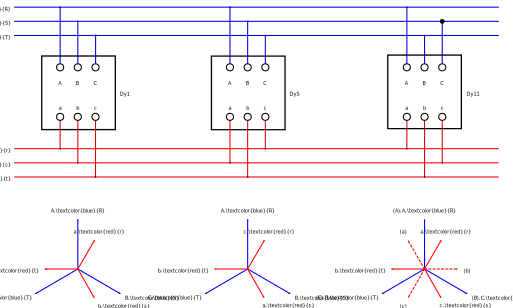
\includegraphics{Imatges/Cap-TrafosPot-Exemple-TR-parallel.pdf}

   \vspace*{1.5cm}
   \hspace{1cm}
   \resizebox{!}{0.8cm}{{\fontfamily{pzc}\selectfont Josep Mollera Barriga}}

\end{titlepage}

      \tableofcontents
      \listoftables
      \listoffigures
      \chapter*{Prefaci} \addcontentsline{toc}{chapter}{Prefaci}

   Voldria dir en primer lloc que no he intentat escriure un tractat complet
   d'electrot\`{e}cnia, d'electr\`{o}nica o de sistemes el\`{e}ctrics de pot\`{e}ncia, sin\'{o} que m\'{e}s aviat
   he volgut
   fer una recopilaci\'{o} de q\"{u}estions te\`{o}riques i pr\`{a}ctiques relacionades amb els camps mencionats
   anteriorment.

   Les fonts d'informaci\'{o} utilitzades en la realitzaci\'{o} d'aquest llibre s\'{o}n molt diverses,
   i inclouen llibres sobre les diferents mat\`{e}ries, articles de revistes o d'Internet,
   apunts de classe d'assignatures impartides a l'\textsf{ETSEIB},\index{ETSEIB} i d'altres.

   Pel que fa al llibre en si mateix, ha estat escrit utilitzant el sistema de composici\'{o} de
   textos \LaTeX,\index{LaTex@\LaTeX} el qual
   permet integrar molt f\`{a}cilment text, f\'{o}rmules i gr\`{a}fics, obtenint un resultat de
   gran qualitat. S'han utilitzat diversos paquets d'ampliaci\'{o}, com ara
   l'\AmS-\LaTeX,\index{AmSLaTex@\AmS-\LaTeX}
   per tal de millorar la presentaci\'{o} de certes parts del
   llibre, com per exemple les taules, les cap\c{c}aleres i les f\'{o}rmules matem\`{a}tiques. S'ha utilitzat la distribuci\'{o} MiK\TeX, que ofereix una implementaci\'{o} lliure de \LaTeX , accessible a l'adre\c{c}a: \href{http://www.miktex.org/}{www.miktex.org}.

   Aquest llibre, est\`{a} pensat per ser utilitzat tant de forma directa en la pantalla d'un
   ordinador com en paper despr\'{e}s d'haver-lo impr\`{e}s; per tal d'estalviar paper, el text
   t\'{e} un format pensat per ser impr\`{e}s en paper DIN-A4,\index{DIN-A4} a dues cares.

    El contingut del llibre \'{e}s molt divers, i va des de temes for\c{c}a te\`{o}rics fins a
    d'altres bastant m\'{e}s pr\`{a}ctics. He procurat donar exemples de tots els conceptes
    que s'hi expliquen, excepci\'{o} feta dels molt elementals, perqu\`{e} crec que \'{e}s important
     no quedar-se tan sols amb la teoria de  la resoluci\'{o} d'un problema determinat, sin\'{o} que
     \'{e}s molt \'{u}til veure exemples resolts pas a pas.

    Encara que he fet tots els esfor\c{c}os possibles per eliminar qualsevol
    mena  d'error en aquest text, \'{e}s gaireb\'{e} inevitable que n'hagi quedat algun,
    per tant, si alg\'{u} troba algun error far\`{a} b\'{e} d'avisar-me!


   \'{U}nicament em resta dir que espero que els que llegeixin aquest llibre el trobin
   \'{u}til i interessant.

\vspace*{1cm}
\hfill
\begin{minipage}[b]{25mm}
    
\includegraphics{Imatges/Pre-Prefaci-JMB.pdf}
\end{minipage}

{\large

\hfill \textbf{\textsl{Josep Mollera Barriga}}

\hfill \textbf{\textsl{Badalona, 24 de mar\c{c} de 2014}}

\hfill \href{mailto:jmollerab@ya.com}{\Letter\hspace{2mm}josep.mollerab@ovi.com}

}

      \fancyhf{} \fancyhead[LE,RO]{\color{NavyBlue}\sffamily\bfseries\thepage}
      \fancyhead[LO,RE]{\color{NavyBlue}\sffamily\bfseries\nouppercase Historial}
      \chapter*{Historial}
\addcontentsline{toc}{chapter}{Historial}

Es presenta a continuaci\'{o} l'evoluci\'{o} que ha tingut aquest llibre, en
les successives versions que han aparegut.

\section*{Versi\'{o} 1.0 (8 de gener de 2005)}
\addcontentsline{toc}{section}{Versi\'{o} 1.0}

Despr\'{e}s de molts esfor\c{c}os, surt a la llum la primera versi\'{o} d'aquest
llibre, format pels cap\'{\i}tols 1, 2, 3, 4, 5, 6 i 7, i els ap\`{e}ndixs A,
B, C, D i E.

\section*{Versi\'{o} 1.1 (8 de febrer de 2005)}
\addcontentsline{toc}{section}{Versi\'{o} 1.1}

S'afegeix al llibre aquest apartat {"<}Historial{">}.

En l'apartat {"<}Notaci\'{o}{">}, s'especifica que el m\`{o}dul d'un nombre
complex \'{e}s igual a l'arrel quadrada \emph{positiva} de la suma dels
quadrats de les seves parts real i imagin\`{a}ria.

Es modifiquen les equacions \eqref{eq:p_3f_34} i \eqref{eq:q_3f_34}.

S'amplia la secci\'{o} corresponent a les difer\`{e}ncies entre les
normatives \textsf{CEI} i \textsf{ANSI}, que fan refer\`{e}ncia als
transformadors de mesura i protecci\'{o} (secci\'{o}
\ref{sec:comp_tt_ti_cei_ansi}).

Es revisa tot el text, fent-hi algunes petites modificacions i
correccions.

\section*{Versi\'{o} 1.2 (16 d'abril de 2005)}
\addcontentsline{toc}{section}{Versi\'{o} 1.2}

En l'apartat {"<}Notaci\'{o}{">}, s'afegeix l'explicaci\'{o} de la convenci\'{o}
seguida a l'hora de dibuixar les fletxes que representen les
tensions i els corrents.

S'afegeix l'ap\`{e}ndix F, on s'explica la designaci\'{o} de les classes de
refrigeraci\'{o} en els transformadors de pot\`{e}ncia.

\section*{Versi\'{o} 1.3 (24 d'octubre de 2005)}
\addcontentsline{toc}{section}{Versi\'{o} 1.3}

Els ap\`{e}ndixs A a F de la versi\'{o} 1.2, es desplacen tres lletres cap
avall, passant a ser els ap\`{e}ndixs D a I respectivament.

S'afegeix un nou ap\`{e}ndix A, dedicat a l'alfabet grec.

S'afegeix un nou ap\`{e}ndix B, dedicat al sistema internacional
d'unitats (SI).

S'afegeix un nou ap\`{e}ndix C, dedicat a les constants f\'{\i}siques.

En l'apartat {"<}Notaci\'{o}{">}, s'amplien les definicions corresponents al
conjugat i al m\`{o}dul d'un nombre complex, i s'inclouen les
definicions de $\mcmplx{V}^*$ i $\hermit{V}$.

S'ha ampliat la secci\'{o} \ref{sec:pot_complex}, corresponent a la
pot\`{e}ncia complexa.

 S'ha ampliat l'exemple de la secci\'{o}
\ref{sec:seccio_pu}.

En la secci\'{o} \ref{sec:EZS}, s'ha afegit el c\`{a}lcul de $R\ped{P}$ i
$\cmplx{Z}\ped{S}$.

 A l'hora de referir-se a la
relaci\'{o} de transformaci\'{o} d'un transformador, se substitueix el
s\'{\i}mbol {"<}$\ddot{u}${">} emprat en les versions anteriors, pel s\'{\i}mbol
{"<}$m${">}.

\section*{Versi\'{o} 1.4 (2 de desembre de 2005)}
\addcontentsline{toc}{section}{Versi\'{o} 1.4}

Es representa correctament la Figura \ref{pic:acobl}, ja que estava
tallada per la dreta.

Es corregeix l'equaci\'{o} \eqref{eq:cdt_trif_exact} i l'exemple que hi
ha a continuaci\'{o}, el qual en fa \'{u}s.

Es revisa tot el text, fent-hi algunes correccions.

\section*{Versi\'{o} 2.0 (3 d'agost de 2006)}
\addcontentsline{toc}{section}{Versi\'{o} 2.0}

S'ha modificat el criteri de colors utilitzat, a l'hora de ressaltar
els enlla\c{c}os interns del document (equacions, p\`{a}gines, etc.) i els
enlla\c{c}os externs; ara els enlla\c{c}os interns s\'{o}n de
\textcolor{red}{color vermell}, i els enlla\c{c}os externs s\'{o}n de
\textcolor{magenta}{color magenta}. A m\'{e}s totes els encap\c{c}alaments
de cap\'{\i}tols, seccions,
 subseccions, taules  i figures, s\'{o}n ara de
 \textcolor{NavyBlue}{color blau}.

S'han afegit nous cap\'{\i}tol i s'ha fet una reordenaci\'{o} que afecta a
diversos cap\'{\i}tols i ap\`{e}ndixs, segons es detalla a continuaci\'{o}:
\begin{dinglist}{'167}
   \item Els cap\'{\i}tols 1 i 2  de la versi\'{o} 1.4 mantenen la seva posici\'{o}.
   \item S'afegeix un nou cap\'{\i}tol 3, on es tracten les s\`{e}ries de Fourier.
   \item S'afegeix un nou cap\'{\i}tol 4, on es tracta la transformada de Laplace.
   \item El cap\'{\i}tol 3 de la versi\'{o} 1.4 es despla\c{c}a dos n\'{u}meros cap
    avall, passant a ser el cap\'{\i}tol 5.
   \item L'ap\`{e}ndix E de la versi\'{o} 1.4 es converteix en el cap\'{\i}tol 6.
   \item Els cap\'{\i}tols 4, 5, 6 i 7  de la versi\'{o} 1.4 es desplacen tres n\'{u}meros cap
    avall, passant a ser els cap\'{\i}tols 7, 8, 9 i 10 respectivament.
    \item L'ap\`{e}ndix G de la versi\'{o} 1.4 es converteix en el cap\'{\i}tol 11.
    \item Els ap\`{e}ndixs A, B, C i D de la versi\'{o} 1.4 mantenen la seva posici\'{o}.
    \item S'afegeix un nou ap\`{e}ndix E, on es tracten relacions trigonom\`{e}triques.
    \item L'ap\`{e}ndix F de la versi\'{o} 1.4 mant\'{e} la seva posici\'{o}.
    \item Els ap\`{e}ndixs H i I de la versi\'{o} 1.4 es desplacen una lletra cap
    amunt, passant a ser els ap\`{e}ndixs G i H respectivament.
\end{dinglist}


 A l'hora de referir-se a la font de corrent i a l'admit\`{a}ncia d'un circuit equivalent
 Norton, se substitueix el sub\'{\i}ndex {"<}Th{">} emprat en les versions
anteriors, pel sub\'{\i}ndex {"<}No{">}.

En l'apartat {"<}Notaci\'{o}{">} s'afegeixen els s\'{\i}mbols: $\mathbb{N}$,
$\mathbb{Z}$, $\mathbb{Z}^+$,  $\mathbb{Z}^*$, $\mathbb{Z}^-$,
$\mathbb{Q}$, $\mathbb{R}$, $\mathbb{R}^+$, $\mathbb{R}^-$ i
$\mathbb{C}$.

S'ha afegit el teorema de la superposici\'{o} en la secci\'{o}
\ref{sec:teoremes}.


S'ha afegit la bateria en la secci\'{o} \ref{sec:comp_elem}, com a un
dels components elementals d'un circuit el\`{e}ctric.

S'ha afegit la secci\'{o} \ref{sec:val_mitja_ef}, on es defineixen els
valors mitj\`{a} i efica\c{c}, i els factors d'amplitud, de forma i
d'arrissada.

S'ha afegit la secci\'{o} \ref{sec:div_tens_corr}, on es tracten els
circuits divisors de tensi\'{o} i divisors de corrent.

 S'ha modificat l'equaci\'{o} \eqref{eq:resistivitat}
i les taules \ref{taula:param-elc} i \ref{taula:AWG}.

S'ha afegit la secci\'{o} \ref{sec:conex_ti_tt}, on s'explica com
connectar correctament transformadors de corrent i de tensi\'{o}, a
aparells de mesura o de protecci\'{o}.

S'ha millorat l'explicaci\'{o} de la secci\'{o} \ref{sec:control-flux-pot}.

S'ha reestructurat la taula \ref{taula:SI-derivades}.

\section*{Versi\'{o} 2.1 (2 de gener de 2007)}
\addcontentsline{toc}{section}{Versi\'{o} 2.1}

S'adopta la compaginaci\'{o} moderna dels par\`{a}grafs en tot el llibre, consistent en separar-los per una l\'{\i}nia en blanc i en no entrar la primera l\'{\i}nia de text.

S'unifica la representaci\'{o} de les fonts de corrent: un cercle amb una fletxa a dins.

S'afegeix una nota a peu de p\`{a}gina en la secci\'{o} \ref{sec:T_N}, relacionant aquesta secci\'{o} amb la secci\'{o} \ref{sec:xarxes_Zth}.

Es millora l'explicaci\'{o} de la secci\'{o} \ref{sec:seccio_pu}, a l'hora que es trasllada de lloc (en les versions anteriors formava part del cap\'{\i}tol \ref{sec:calc_bas}).

Es millora l'explicaci\'{o} de la secci\'{o} \ref{sec:comp-sim-neutre}.

S'afegeix una nota a peu de p\`{a}gina en la secci\'{o} \ref{sec:EZS}, relacionant aquesta secci\'{o} amb el cap\'{\i}tol \ref{chap:flux_carregues}.

S'amplia la descripci\'{o} de l'equaci\'{o} \eqref{eq:awg_mm2}.

S'afegeix la secci\'{o} \ref{sec:sis_eq_no_lin}, on s'explica com resoldre sistemes d'equacions no lineals amb els programes \textit{Mathematica}${}^\circledR$ i \textit{MATLAB}${}^\circledR$.

Es millora l'explicaci\'{o} de la secci\'{o} \ref{sec:llei-s-c-t}, modificant la figura \ref{pic:llei-s-c-t} i numerant l'equaci\'{o} de la llei dels sinus.

\section*{Versi\'{o} 2.2 (10 de mar\c{c} de 2008)}
\addcontentsline{toc}{section}{Versi\'{o} 2.2}

Es canvia el color dels enlla\c{c}os interns, passant a ser de color negre com el text.

S'afegeixen les unitats que mancaven en alguns exemples.

En la secci\'{o} \ref{sec:MCM} s'introdueixen les unitats cmil i kcmil, equivalents a les unitats CM i MCM respectivament. Avui en dia \'{e}s m\'{e}s freq\"{u}ent veure escrit cmil i kcmil.

Es revisa l'ap\`{e}ndix B utilitzant les publicacions de l'any 2006 del {"<}Bureau
International des Poids et Mesures{">} (\textsf{BIPM}).\index{BIPM}

Es revisa l'ap\`{e}ndix C utilitzant les publicacions de l'any 2006 del {"<}Committee on Data for Science and Technology{">} (\textsf{CODATA}).\index{CODATA}

\section*{Versi\'{o} 3.0 (1 d'octubre de 2008)}
\addcontentsline{toc}{section}{Versi\'{o} 3.0}

Els cap\'{\i}tols 9, 10 i 11 de la versi\'{o} 2.2, es desplacen un n\'{u}mero cap
avall, passant a ser els cap\'{\i}tols 10, 11 i 12 respectivament.

Es crea un nou cap\'{\i}tol 9, dedicat als transformadors de pot\`{e}ncia;
l'ap\`{e}ndix H de la versi\'{o} 2.2 desapareix com a tal, quedant integrat
dins d'aquest nou cap\'{\i}tol.


\section*{Versi\'{o} 3.1 (5 de desembre de 2009)}
\addcontentsline{toc}{section}{Versi\'{o} 3.1}
En l'Ap\`{e}ndix B s'afegeixen els prefixes de pot\`{e}ncies bin\`{a}ries Ki, Mi, Gi, Ti, Pi i Ei.

Es revisa tot el text, fent-hi algunes petites modificacions i
correccions.

\section*{Versi\'{o} 3.2 (5 de gener de 2010)}
\addcontentsline{toc}{section}{Versi\'{o} 3.2}
S'afegeix l'apartat Bibliografia despr\'{e}s del ap\`{e}ndixs. 
     \fancyhf{} \fancyhead[LE,RO]{\color{NavyBlue}\sffamily\bfseries\thepage}
      \fancyhead[LO,RE]{\color{NavyBlue}\sffamily\bfseries\nouppercase Notaci\'{o}}
      \chapter*{Notació} \addcontentsline{toc}{chapter}{Notació}

\section*{Variables} \addcontentsline{toc}{section}{Variables}


En aquest llibre les variables escalars s'escriuen en lletra  de gruix normal, i  les variables vectorials i matricials s'escriuen
en lletra negreta.

\begin{list}{}
{\setlength{\labelwidth}{15mm} \setlength{\leftmargin}{20mm}
\setlength{\labelsep}{5mm}}
    \item[$j$] La unitat imaginària, definida com:
    $j\equiv\sqrt{-1}$\index{j@$j$}
    \item[$V$] Una variable real.
    \item[$\cmplx{V}$] Una variable complexa.
    \item[$\cmplx{V}^*$] Conjugat d'una variable complexa.
    Es compleixen les relacions:\\[1ex]
     $(\cmplx{V}_1 \pm \cmplx{V}_2 \pm \cdots  \pm \cmplx{V}_n)^* = \cmplx{V}_1^* \pm
    \cmplx{V}_2^*\pm\cdots\pm\cmplx{V}_n^*$\\[1ex]
    $(\cmplx{V}_1 \cmplx{V}_2 \cdots \cmplx{V}_n)^* = \cmplx{V}_1^*  \cmplx{V}_2^*
    \cdots \cmplx{V}_n^*$\\[1ex]
    $(\cmplx{V}_1 / \cmplx{V}_2)^* = \cmplx{V}_1^* / \cmplx{V}_2^*$
    \item[$|\cmplx{V}|$] Mòdul d'una variable complexa.
    Es compleixen les relacions:\\[1ex]
      $\cmplx{V}\,\cmplx{V}^* = |\cmplx{V}|^2$\\[1ex]
      $1/ \cmplx{V} = \cmplx{V}^* / \,|\cmplx{V}|^2$\\[1ex]
      $|\cmplx{V}_1 \cmplx{V}_2 \cdots \cmplx{V}_n| =
       |\cmplx{V}_1| \,|\cmplx{V}_2| \cdots |\cmplx{V}_n|$\\[1ex]
       $|\cmplx{V}_1 / \cmplx{V}_2| = |\cmplx{V}_1| \,/ \,|\cmplx{V}_2|$\\[1ex]
      $|\cmplx{V}_1+\cmplx{V}_2+\cdots+\cmplx{V}_n| \leq
      |\cmplx{V}_1| + |\cmplx{V}_2| + \cdots  +|\cmplx{V}_n|$
    \item[$\arg\cmplx{V}$] Argument (angle) d'una variable complexa.
     Es compleixen les relacions:\\[1ex]
      $\arg\cmplx{V}^* = - \arg\cmplx{V}$\\[1ex]
      $\arg(-\cmplx{V}) =  \arg\cmplx{V} + \piup$\\[1ex]
      $\arg(\cmplx{V}_1 \cmplx{V}_2 \cdots \cmplx{V}_n) = \arg\cmplx{V}_1 + \arg \cmplx{V}_2 + \cdots + \arg\cmplx{V}_n$\\[1ex]
      $\arg(\cmplx{V}_1 / \cmplx{V}_2) = \arg\cmplx{V}_1 - \arg \cmplx{V}_2$
    \item[$\Re\cmplx{V}$] Part real d'una variable complexa. Es compleix: $\Re\cmplx{V} = \dfrac{\cmplx{V} + \cmplx{V}^*}{2}$
    \item[$\Im\cmplx{V}$] Part imaginària d'una variable complexa. Es compleix: $\Im\cmplx{V} = \dfrac{\cmplx{V} - \cmplx{V}^*}{2 j}$
    \item[$A+j B$] Expressió cartesiana (part real i part
    imaginària) d'una variable complexa.
    \item[$Z\angle\theta$] Expressió polar (mòdul i argument) d'una variable
    complexa. Les relacions entre $A, B, Z$ i $\theta$ són:\footnote{Cal tenir en compte que la funció \texttt{arctan} disponible en moltes calculadores i llenguatges de programació, torna de forma  estandarditzada valors compresos entre $-\frac{\piup}{2}$ i $\frac{\piup}{2}$. En aquest cas cal sumar el valor $\piup$, quan $A$ és negatiu, a l'angle obtingut amb la funció \texttt{arctan} per tal d'obtenir l'angle en el quadrant correcte.}\\[1ex]
    $Z=+\sqrt{A^2+B^2}\qquad\quad\theta=\arctan{\dfrac{B}{A}}\qquad\quad
    A=Z\cos\theta\qquad\quad B=Z\sin\theta$
    \item[$Z\,e^{j\theta}$] Expressió d'Euler\index{Euler} d'una variable complexa, definida com:\footnote{El valor de $\theta$ ha d'expressar-se sempre en radian, per tal que el valor de $e^{j\theta}$ sigui correcte.}
     $Z\,e^{j\theta} \equiv Z(\cos\theta+j\sin\theta)$.
     Es compleixen les relacions:\\[1ex]
     $Z_1\,e^{j\theta_1} \, Z_2\,e^{j\theta_2} = Z_1 Z_2\,e^{j(\theta_1+\theta_2)}$\\[1ex]
     %$(Z_1\,e^{j\theta_1}) \,/\, (Z_2\,e^{j\theta_2}) = \dfrac{Z_1}{Z_2}\,e^{j(\theta_1-\theta_2)}$
     $\dfrac{Z_1\,e^{j\theta_1}}{Z_2\,e^{j\theta_2}} = \dfrac{Z_1}{Z_2}\,e^{j(\theta_1-\theta_2)}$
    \item[$\boldsymbol{V}$] Una matriu real o un vector real.
    \item[$\boldsymbol{V}^{-1}$] Matriu inversa d'una matriu real.
    \item[$\transpose{\boldsymbol{V}}$] Matriu transposada d'una matriu real, o vector
    transposat d'un vector real.
    \item[$\boldsymbol{V}(n)$] Element $n$-èsim d'un vector real.
    \item[$\boldsymbol{V}(m,n)$] Element de la fila $m$ i columna $n$ d'una matriu real.
    \item[$\mcmplx{V}$] Una matriu complexa o un vector complex.
    \item[$\mcmplx{V}^{-1}$] Matriu inversa d'una matriu complexa.
    \item[$\transpose{\mcmplx{V}}$] Matriu transposada d'una matriu complexa, o vector
    transposat d'un vector complex.
    \item[$\mcmplx{V}^*$] Matriu conjugada d'una matriu complexa, o vector
    conjugat d'un vector complex.
    \item[$\hermit{V}$] Matriu conjugada transposada d'una matriu complexa, o vector
    conjugat transposat d'un vector complex, definit com: $\hermit{V} \equiv
    \transpose{(\mcmplx{V}^*)}$.
    \item[$\mcmplx{V}(n)$] Element $n$-èsim d'un vector complex.
    \item[$\mcmplx{V}(m,n)$] Element de la fila $m$ i columna $n$ d'una matriu complexa.
\end{list}

Pel que fa als sentits assignats a les fletxes que representen les
tensions i els corrents en els diversos circuits elèctrics que
apareixen en aquest llibre, s'utilitza la convenció següent:

\begin{list}{}
{\setlength{\labelwidth}{15mm} \setlength{\leftmargin}{20mm}
\setlength{\labelsep}{5mm}}
    \item[$\begin{CD} @>U>> \end{CD}$] Tensió contínua: la fletxa indica el sentit
    de la caiguda de tensió, és a dir, va del nus positiu al nus negatiu.
    \item[$\begin{CD} @>I>> \end{CD}$] Corrent
    continu: la fletxa indica el sentit  assignat com a positiu al corrent.
    \item[$\begin{CD} @>\cmplx{U}>> \end{CD}$] Tensió alterna: la fletxa indica el
    sentit assignat com a positiu a la caiguda de tensió, quan el nus d'origen de la fletxa
    té un potencial  més positiu que el nus de destinació.
    \item[$\begin{CD} @>\cmplx{I}>> \end{CD}$] Corrent altern: la fletxa
    indica el sentit  assignat com a positiu al corrent.
\end{list}

\section*{Fasors} \addcontentsline{toc}{section}{Fasors}

En aquest llibre les variables complexes s'utilitzen per representar fasors. Un fasor $Z\angle\theta$ és equivalent a una funció sinusoidal variable en el temps, la qual pot expressar-se utilitzant la funció cosinus:
\[y(t)=\sqrt{2}\, Z \cos(\omega t + \theta)\]

o utilitzant la funció sinus:
\[y(t)=\sqrt{2}\, Z \sin(\omega t + \theta)\]

Quan hi ha diverses funcions sinusoidals relacionades entre si, cal utilitzar de manera uniforme la funció cosinus o la funció sinus per a totes les funcions. Les variables i paràmetres implicats són:
\begin{list}{}
{\setlength{\labelwidth}{15mm} \setlength{\leftmargin}{20mm}
\setlength{\labelsep}{5mm}}
    \item[$y(t)$] Funció sinusoidal; representa normalment una tensió o un corrent.
    \item[$t$] Temps.
    \item[$f$] Freqüència de la funció sinusoidal.
    \item[$T$] Període de la funció sinusoidal.
    \item[$\omega$] Velocitat angular de la funció sinusoidal. Es compleix: $\omega = 2 \piup f = 2 \piup/T$.
    \item[$Z$] Valor eficaç de la funció sinusoidal (vegeu la secció \vref{sec:val_mitja_ef}); els valors de pic de la funció sinusoidal  són:  $\pm\sqrt{2}\, Z$.
    \item[$\theta$] Angle inicial de la funció sinusoidal, on  $\theta=\omega \tau = -\omega (T-\tau)$; el significat del temps $\tau$  es pot veure en el gràfic que hi ha més avall.

    Quan es fa servir la funció cosinus, $\theta$ és positiu quan s'utilitza $\tau$, és a dir, el temps mesurat  des de l'origen ($t=0$) cap a l'esquerra, fins a trobar el primer valor màxim de la funció, i $\theta$ és negatiu quan s'utilitza $T-\tau$, és a dir, el temps mesurat des de l'origen cap a la dreta, fins a trobar també el primer valor màxim de la funció.

    Quan es fa servir la funció sinus, $\theta$ és positiu quan s'utilitza $\tau$, és a dir, el temps mesurat des de l'origen ($t=0$) cap a l'esquerra, fins a trobar el primer punt on la funció es fa zero (passant de valors negatius a positius), i $\theta$ és negatiu quan s'utilitza $T-\tau$, és a dir, el temps mesurat des de l'origen cap a la dreta, fins a trobar també el primer punt on la funció es fa zero (passant de valors negatius a positius).
    \item[] \input{Imatges/Not-Fasor.pdf_tex}
\end{list}
\index{fasor}

\section*{Conjunts de nombres i intervals} \addcontentsline{toc}{section}{Conjunts de nombres i intervals}

Els símbols que representen els diferents conjunts de nombres i intervals, segons la norma internacional ISO 80000-2 
\textit{Quantities and units --- Part 2: Mathematics}, són els següents:

\begin{list}{}
{\setlength{\labelwidth}{15mm} \setlength{\leftmargin}{20mm}
\setlength{\labelsep}{5mm}}
	 \item[$\mathsfb{N}$] Conjunt dels nombres naturals: $\{\,0,1,2,3,4,\ldots\,\}$. 
	 
	 L'exclusió del zero s'indica amb un asterisc: $\mathsfb{N}^* = \{ n \in \mathsfb{N} \mid n \ne 0 \}$. 
	 
	 És possible indicar altres restriccions, com per exemple:  $\mathsfb{N}_{> 5} = \{ n \in \mathsfb{N} \mid n > 5\}$. 
	 
	 També s'utilitzen els símbols $\vmathbb{N}$ i  $\vvmathbb{N}$.
	 
	 \item[$\mathsfb{Z}$] Conjunt dels nombres enters: $\{\,\ldots,-3,-2,-1,0,1,2,3,\ldots\,\}$.  
	 
	 L'exclusió del zero s'indica amb un asterisc: $\mathsfb{Z}^* = \{ n \in \mathsfb{Z} \mid n \ne 0 \}$. 
	 
	 És possible indicar altres restriccions, com per exemple:  $\mathsfb{Z}_{> -3} = \{ n \in \mathsfb{Z} \mid n > -3\}$.     
	 
	 També s'utilitzen els símbols $\vmathbb{Z}$ i $\vvmathbb{Z}$.
    
	 \item[$\mathsfb{Q}$] Conjunt dels nombres racionals. 
	 
	 L'exclusió del zero s'indica amb un asterisc: $\mathsfb{Q}^* = \{ r \in \mathsfb{Q} \mid r \ne 0 \}$. 
	 
	 És possible indicar altres restriccions, com per exemple:  $\mathsfb{Q}_{< 0} = \{ r \in \mathsfb{Q} \mid r < 0 \}$. 
	 
	 També s'utilitzen els símbols $\vmathbb{Q}$ i $\vvmathbb{Q}$.
	 
	 \item[$\mathsfb{R}$] Conjunt dels nombres reals. 
	 
	 L'exclusió del zero s'indica amb un asterisc: $\mathsfb{R}^* = \{ x \in \mathsfb{R} \mid x \ne 0 \}$. 
	 
	 És possible indicar altres restriccions, com per exemple:  $\mathsfb{R}_{> 0} = \{ x \in \mathsfb{R} \mid x > 0 \}$. 
	 
	 També s'utilitzen els símbols $\vmathbb{R}$ i $\vvmathbb{R}$.
	 
	\item[$\mathsfb{C}$] Conjunt dels nombres complexos.  
	
	L'exclusió del zero s'indica amb un asterisc: $\mathsfb{C}^* = \{ z \in \mathsfb{C} \mid z \ne 0 \}$.
	
	 També s'utilitzen els símbols $\vmathbb{C}$ i $\vvmathbb{C}$.
	 
	 \item[$\mathsfb{P}$] Conjunt dels nombres primers: $\{\,2,3,5,7,11,13,17,19,23,29,31,37,41,43,47,53,59,61,\ldots\,\}$. 
	 
	 També s'utilitzen els símbols $\vmathbb{P}$ i $\vvmathbb{P}$.
	 
	 \item[{$[a,b]$}] Interval tancat des de $a$ inclòs fins a $b$ inclòs: $[a,b] = \{x \in \mathsfb{R} \mid a \leq x \leq b\}$.
	 
	 \item[{$(a,b]$}] Interval semiobert esquerre des de $a$ exclòs fins a $b$ inclòs: $(a,b] = \{x \in \mathsfb{R} \mid a < x \leq b\}$. 
	 
	 També s'utilitza la notació $]a,b]$.
	 
	 \item[{$[a,b)$}] Interval semiobert dret des de $a$ inclòs fins a $b$ exclòs: $[a,b) = \{x \in \mathsfb{R} \mid a \leq x < b\}$. 
	 
	 També s'utilitza la notació $[a,b[$.
	 
	 \item[{$(a,b)$}] Interval obert des de $a$ exclòs fins a $b$ exclòs: $(a,b) = \{x \in \mathsfb{R} \mid a < x < b\}$. 
	 
	 També s'utilitza la notació $]a,b[$.
	 
	 \item[{$(-\infty,b]$}] Interval iŀlimitat tancat fins a $b$ inclòs: $(-\infty,b] = \{x \in \mathsfb{R} \mid x \leq b\}$.  
	 
	 També s'utilitza la notació $]-\infty,b]$.
	 
	 \item[{$(-\infty,b)$}] Interval iŀlimitat obert fins a $b$ exclòs: $(-\infty,b) = \{x \in \mathsfb{R} \mid x < b\}$. 
	 
	 També s'utilitza la notació $]-\infty,b[$.
	 
	 \item[{$[a,+\infty)$}] Interval iŀlimitat tancat des de $a$ inclòs: $[a, +\infty) = \{x \in \mathsfb{R} \mid  x \geq a\}$. 
	 
	 També s'utilitzen les notacions $[a, \infty)$, $[a, +\infty[$ i $[a, \infty[$.

	\item[{$(a,+\infty)$}] Interval iŀlimitat obert des de $a$ exclòs: $(a, +\infty) = \{x \in \mathsfb{R} \mid  x > a\}$. 
	
	També s'utilitzen les notacions $(a, \infty)$, $]a, +\infty[$ i $]a, \infty[$.
\end{list}
\index{N@$\mathsfb{N}$} \index{N@$\mathsfb{N}^*$}
\index{Z@$\mathsfb{Z}$} \index{Z@$\mathsfb{Z}^*$}
\index{Q@$\mathsfb{Q}$} \index{Q@$\mathsfb{Q}^*$}
\index{R@$\mathsfb{R}$} \index{R@$\mathsfb{R}^*$}
\index{C@$\mathsfb{C}$} \index{C@$\mathsfb{C}^*$}
\index{P@$\mathsfb{P}$}


\section*{Alfabet grec} \addcontentsline{toc}{section}{Alfabet grec}
\index{alfabet grec}

A continuació es pot veure l'alfabet grec
amb els noms de les seves lletres en diversos idiomes. Algunes lletres minúscules tenen dues grafies, totalment equivalents entre sí.

\begin{center}
\begin{threeparttable}
	\begin{tabular}{cccllll}
		\toprule[1pt]
		\renewcommand*{\multirowsetup}{\centering}
		\multirow{2}{15mm}{\rule{0mm}{4.5mm}Número\\d'ordre} & \multicolumn{2}{c}{Lletra} &
		\multicolumn{4}{c}{Nom} \\
		\cmidrule(rl){2-3} \cmidrule(rl){4-7}
		& minúscula & majúscula & català & castellà &  anglès & francès\\
		\midrule
		1  & $\alphaup$ & A & alfa & alfa &  alpha & alpha\\
		2  & $\betaup$ & B & beta & beta &  beta & bêta\\
		3  & $\gammaup$ & $\Gammaup$ & gamma & gamma &  gamma & gamma\\
		4  & $\deltaup$ & $\Deltaup$ & delta & delta &  delta & delta\\
		5  & $\epsilonup$, $\varepsilonup$ & E & èpsilon & épsilon &  epsilon & epsilon\\
		6  & $\zetaup$ & Z & zeta & dseta &  zeta & zêta\\
		7  & $\etaup$ & H & eta & eta &  eta & êta\\
		8  & $\thetaup$, $\varthetaup$ & $\Thetaup$ & theta & zeta &  theta & thêta\\
		9  & $\iotaup$ & I & iota & iota &  iota & iota\\
		10 & $\kappaup$, $\varkappaup$ & K & kappa & kappa &  kappa & kappa\\
		11 & $\lambdaup$ & $\Lambdaup$ & lambda & lambda &  lambda &lambda\\
		12 & $\muup$ & M & mi & mi &  mu & mu\\
		13 & $\nuup$ & N & ni & ni &  nu & nu\\
		14 & $\xiup$ & $\Xiup$ & ksi & xi &  xi & ksi, xi\\
		15 & o & O & òmicron & ómicron &  omicron & omicron\\
		16 & $\piup$, $\varpiup$\tnote{\color{blue}(a)} & $\Piup$ & pi & pi &  pi & pi\\
		17 & $\rhoup$, $\varrhoup$ & P & rho, ro & ro &  rho & rhô\\
		18 & $\sigmaup$, $\varsigmaup$\tnote{\color{blue}(b)} & $\Sigmaup$ & sigma & sigma &  sigma &sigma\\
		19 & $\tauup$ & T & tau & tau & tau &tau\\
		20 & $\upsilonup$ & $\Upsilonup$ & ípsilon & ípsilon &  upsilon &upsilon\\
		21 & $\phiup$, $\varphiup$ & $\Phiup$ & fi & fi &  phi & phi\\
		22 & $\chiup$ & X & khi & ji &  chi & khi\\
		23 & $\psiup$ & $\Psiup$ & psi & psi &  psi & psi\\
		24 & $\omegaup$ & $\Omegaup$ & omega & omega &  omega & oméga\\
		\bottomrule[1pt]
	\end{tabular}
	\begin{tablenotes}
		\item[\color{blue}(a)] {\footnotesize La variant $\varpiup$ de la lletra pi, que no es fa servir en textos tècnics i científics, es denomina «pi dòrica» en  català, «pi dórica» en castellà, «dorian pi» en anglès, i «pi dorien» en francès.}
		\item[\color{blue}(b)] {\footnotesize En grec, la variant $\varsigmaup$ de la lletra sigma s'escriu  al final d'una paraula, i la variant $\sigmaup$  a l'inici o en mig d'una paraula. En els textos tècnics i científics s'utilitza  la variant $\sigmaup$.}
	\end{tablenotes}
\end{threeparttable}
\end{center}



Els noms d'algunes lletres poden sorprendre, ja que n'hi ha que han rebut històricament noms
diversos, i fins i tot contradictoris respecte dels actuals.

Els noms anglesos de les lletres són els més uniformes, ja que no
s'ha observat cap variació en les diverses fonts consultades, essencialment el diccionari nord-americà Merriam-Webster\footnote{Aquest diccionari es pot consultar a l'adreça: \href{https://www.merriam-webster.com/}{https://www.merriam-webster.com}.} i els diccionaris britànics Oxford\footnote{Aquest diccionari es pot consultar a l'adreça: \href{https://www.oed.com/}{https://www.oed.com}.} i Cambridge.\footnote{Aquest diccionari es pot consultar a l'adreça: \href{https://dictionary.cambridge.org/}{https://dictionary.cambridge.org}.}

Els noms catalans de les lletres són els que apareixen en el \textit{Diccionari de la llengua catalana, 2a edició, 2007} (DIEC2).\footnote{Aquest diccionari es pot consultar a l'adreça: \href{http://dlc.iec.cat/}{https://dlc.iec.cat}. La versió en línia s'actualitza periòdicament.} Altres noms utilitzats en
les diverses fonts consultades, que actualment estan fora de la norma ortogràfica, són:
\begin{multicols}{3}
	\begin{list}{}
		{\setlength{\labelwidth}{16mm} \setlength{\leftmargin}{16mm} \setlength{\labelsep}{2mm}}
		\item[B, $\betaup :$] vita.
		\item[Z, $\zetaup :$] zita.
		\item[H, $\etaup :$] ita.
		\item[$\Thetaup$, $\thetaup :$] thita.
		\item[T, $\tauup :$] taf.
		\item[$\xiup$, $\Xiup$:] csi.\footnote{El nom «csi» apareix juntament amb «ksi» en el \textit{Gran Diccionari de la Llengua Catalana (1999)}. Aquest diccionari es pot consultar a l'adreça:  \href{https://www.diccionari.cat/}{https://www.diccionari.cat}.}
	\end{list}
\end{multicols}

Els noms castellans de les lletres són els que apareixen en el \textit{Diccionario de la Lengua Española, 23ª
	edición, 2014} (D.R.A.E.).\footnote{Aquest diccionari es pot consultar a l'adreça:  \href{https://www.rae.es/}{https://www.rae.es}. La versió en línia s'actualitza periòdicament.} Altres noms utilitzats en les diverses fonts
consultades, que actualment estan fora de la norma ortogràfica, són:
\begin{multicols}{3}
	\begin{list}{}
		{\setlength{\labelwidth}{16mm} \setlength{\leftmargin}{16mm} \setlength{\labelsep}{2mm}}
		\item[Z, $\zetaup :$] zeta,\footnote{\label{fn:zeta}Els noms «zeta», «theta», «my» i «ny» eren els que apareixien en les edicions
			del D.R.A.E anteriors a la 21a (1992).} dseda,\footnote{El nom «dseda» era el que apareixia en l'edició 22a (2001) del D.R.A.E.} dzeta.
		\item[$\Thetaup$, $\thetaup :$] theta,\footnoteref{fn:zeta} thita.
		\item[K, $\kappaup :$] cappa.
		\item[M, $\muup :$] my,\footnoteref{fn:zeta} mu.
		\item[N, $\nuup :$] ny,\footnoteref{fn:zeta} nu.
		\item[O, o :] omicrón.
		\item[P, $\rhoup :$] rho.
		\item[$\Upsilonup$, $\upsilonup :$] úpsilon.
		\item[$\Phiup$, $\phiup :$] phi.
	\end{list}
\end{multicols}

Els noms francesos de les lletres són els que apareixen en el \textit{Dictionnaire de l'Académie française, neuvième édition}.\footnote{Aquest diccionari es pot consultar a l'adreça: \href{https://www.academie-francaise.fr/le-dictionnaire/la-9e-edition}{https://www.academie-francaise.fr/le-dictionnaire/la-9e-edition}.} 
   \mainmatter
      % estil de les p\`{a}gines normals parells i senars
      \renewcommand{\chaptermark}[1]{\markboth{\chaptername\ \thechapter.\ #1}{}}
      \renewcommand{\sectionmark}[1]{\markright{\thesection\ #1}}
      \fancyhf{} \fancyhead[LE,RO]{\color{NavyBlue}\sffamily\bfseries\thepage}
      \fancyhead[LO]{\color{NavyBlue}\sffamily\bfseries\nouppercase\rightmark}
      \fancyhead[RE]{\color{NavyBlue}\sffamily\bfseries\nouppercase\leftmark}
   \part{Electrot\`{e}cnia}
      \chapter{Fonaments}

\section{Introducció}
Es tracten en aquest capítol qüestions bàsiques
d'electrotècnia, com ara teoremes, definicions i relacions, components elementals, i circuits bàsics.


\section{Teoremes d'electrotècnia}\label{sec:teoremes}

\subsection{\texorpdfstring{Teorema de Thévenin--Norton}{Teorema de
            Thévenin-Norton}}\label{sec:T_N}

\index{teorema!de Thévenin}El teorema de Thévenin ens permet
substituir una xarxa complexa formada per elements lineals, per un
circuit equivalent format per una font de tensió $\cmplx{E}\ped{Th}$
en sèrie amb una impedància $\cmplx{Z}\ped{Th}$.


Atenent a la Figura \vref{pic:Thevenin}, si coneixem la tensió en
buit $\cmplx{U}\ped{o}$ entre dos nusos $\alphaup$ i $\betaup$ d'una
xarxa, i la impedància $\cmplx{Z}_{\alphaup\betaup}$ d'aquesta xarxa
vista des d'aquests dos nusos, podem obtenir els valors del circuit
Thévenin equivalent entre aquests dos nusos a partir de les
relacions següents:\index{ETh@$E\ped{Th}$}\index{ZTh@$Z\ped{Th}$}
\begin{equation}
   \cmplx{E}\ped{Th} = \cmplx{U}\ped{o} \qquad\qquad  \cmplx{Z}\ped{Th} = \cmplx{Z}_{\alphaup\betaup}
\end{equation}

D'aquesta manera, la connexió d'aquesta xarxa a través dels nusos
$\alphaup$ i $\betaup$ a una càrrega qualsevol $\cmplx{Z}\ped{Q}$, és
equivalent pel que fa a aquesta càrrega, a connectar-la al circuit
equivalent Thévenin.
\begin{center}
    \input{Imatges/Cap-Fonaments-Thevenin.pdf_tex}
    \captionof{figure}{Teorema de Thévenin}
    \label{pic:Thevenin}
\end{center}

\index{teorema!de Norton}El teorema de Norton ens permet substituir
una xarxa complexa formada per elements lineals, per un circuit
equivalent format per una font de corrent $\cmplx{J}\ped{No}$ en
paraŀlel amb una admitància $\cmplx{Y}\ped{No}$.

Atenent a la Figura \vref{pic:Norton}, si coneixem el corrent de
curtcircuit $\cmplx{I}\ped{cc}$ entre dos nusos $\alphaup$ i $\betaup$
d'una xarxa, i l'admitància $\cmplx{Y}_{\alphaup\betaup}$ d'aquesta
xarxa vista des d'aquests dos nusos, podem obtenir els valors del
circuit Norton equivalent entre aquests dos nusos a partir de les
relacions següents:\index{JNo@$J\ped{No}$}\index{YNo@$Y\ped{No}$}
\begin{equation}
   \cmplx{J}\ped{No} = \cmplx{I}\ped{cc} \qquad\qquad \cmplx{Y}\ped{No} = \cmplx{Y}_{\alphaup\betaup}
\end{equation}

D'aquesta manera, la connexió d'aquesta xarxa a través dels nusos
$\alphaup$ i $\betaup$ a una càrrega qualsevol $\cmplx{Z}\ped{Q}$, és
equivalent pel que fa a aquesta càrrega, a connectar-la al circuit
equivalent Norton.
\begin{center}
    \input{Imatges/Cap-Fonaments-Norton.pdf_tex}
    \captionof{figure}{Teorema de Norton}
    \label{pic:Norton}
\end{center}

Els circuits Thévenin i Norton d'una xarxa són equivalents entre si.
Els paràmetres que defineixen aquests dos circuits compleixen les relacions
següents:
\begin{equation}\label{eq:Thevenin-Norton}
   \cmplx{E}\ped{Th} = \frac{\cmplx{J}\ped{No}}{\cmplx{Y}\ped{No}} \qquad\qquad
   \cmplx{J}\ped{No} = \frac{\cmplx{E}\ped{Th}}{\cmplx{Z}\ped{Th}} \qquad\qquad
    \cmplx{Z}\ped{Th} = \frac{1}{\cmplx{Y}\ped{No}}
\end{equation}

Els valors $\cmplx{Z}\ped{Th}$ i  $\cmplx{Y}\ped{No}$ es poden
obtenir substituint en la xarxa  les fonts de tensió  per curtcircuits, i les fonts de corrent per circuits oberts, i calculant
aleshores la impedància o admitància equivalent\footnote{El càlcul sistemàtic de $\cmplx{Z}\ped{Th}$ i  $\cmplx{Y}\ped{No}$ en una xarxa qualsevol, s'exposa en la secció \ref{sec:xarxes_Zth}}.

\subsection{Teorema de Millman}\label{sec:millman}

\index{teorema!de Millman}Atenent a la Figura \vref{pic:Millman}, el teorema
de Millman ens permet
obtenir la tensió de l'extrem comú $\nuup$ de diverses impedàncies respecte d'un punt
qualsevol $\alphaup$, a partir de les tensions dels altres extrems de les impedàncies respecte
 del mateix punt $\alphaup$.

\hfill
\begin{minipage}[b]{7cm}
    \input{Imatges/Cap-Fonaments-Millman.pdf_tex}
    \captionof{figure}{Teorema de Millman}
    \label{pic:Millman}
\end{minipage}
\hfill
\begin{minipage}[b][4.5cm][t]{6cm}
    \begin{equation}
        \cmplx{U}_{\nuup\alphaup} = \frac{\displaystyle\sum_{k=1}^n \dfrac{\cmplx{U}_{k\alphaup}}{\cmplx{Z}_k}} {\displaystyle\sum_{k=1}^n \dfrac{1}{\cmplx{Z}_k}}
    \end{equation}
\end{minipage}


\pagebreak

\begin{exemple}[Teorema de Millman -- Bateries en paraŀlel]
    A partir de la figura següent, es tracta de determinar els circuits
    Thévenin i Norton equivalents del circuit format per les tres
    bateries i les seves resistències, i calcular la tensió i el
    corrent que existirien en una resistència de càrrega
    $R\ped{Q}=\SI{50}{\ohm}$, que es connectés entre els punts $\alphaup$
    i $\nuup$.

    \begin{center}
        \input{Imatges/Cap-Fonaments-Millman-Exemple1.pdf_tex}
    \end{center}

    La impedància Thévenin equivalent es calcula, tal com s'ha dit en la Secció \ref{sec:T_N},
    substituint en el circuit totes les fonts de tensió per curtcircuits; així doncs, ens
    queden tres resistències en paraŀlel entre $\alphaup$ i $\nuup$:
    \[
    Z\ped{Th} = \frac{1}{\dfrac{1}{\SI{0,034}{\ohm}} +
    \dfrac{1}{\SI{0,041}{\ohm}} + \dfrac{1}{\SI{0,029}{\ohm}}} =
    \SI{0,01133}{\ohm}
    \]

    Per calcular la font de tensió Thévenin equivalent, utilitzarem el
    teorema de Millman. Si es compara aquest circuit amb el de la Figura
    \vref{pic:Millman}, veiem que els punts $\alphaup$ i $\nuup$ dels dos
    circuits són equivalents, és a dir, $\nuup$ és el punt comú de les
    impedàncies, i $\alphaup$ és el punt de referència dels altres extrems
    de les impedàncies, respecte del qual les tensions són conegudes
    (tensions de les bateries). Així doncs tenim:
    \[
    U_{\nuup\alphaup} = \frac{\dfrac{\SI{-125,1}{V}}{\SI{0,034}{\ohm}} +
    \dfrac{\SI{-124,8}{V}}{\SI{0,041}{\ohm}} +
    \dfrac{\SI{-125,2}{V}}{\SI{0,029}{\ohm}}}{\dfrac{1}{\SI{0,034}{\ohm}}
    + \dfrac{1}{\SI{0,041}{\ohm}} + \dfrac{1}{\SI{0,029}{\ohm}}} =
    \SI{-125,0562}{V}
    \]

    La font de tensió  Thévenin equivalent entre $\alphaup$ i $\nuup$ és per
    tant:
    \[
    E\ped{Th} = U_{\alphaup\nuup} = \SI{125,0562}{V}
    \]

    Calculem a continuació l'admitància i la font de corrent  Norton equivalents, utilitzant
    l'equació \eqref{eq:Thevenin-Norton}:
    \begin{align*}
        Y\ped{No} &= \frac{1}{Z\ped{Th}} = \frac{1}{\SI{0,01133}{\ohm}} = \SI{82,2613}{S}
        \\[2ex]
        J\ped{No} &= \frac{E\ped{Th}}{Z\ped{Th}} =
        \frac{\SI{125,0562}{V}}{\SI{0,01133}{\ohm}}= \SI{11037,6150}{A}
    \end{align*}

    Tal com s'ha dit en la Secció \ref{sec:T_N}, J\ped{No} és igual al
    corrent de curtcircuit entre els punts $\alphaup$ i $\nuup$.

    Finalment, ja podem calcular el corrent $I\ped{Q}$ i la tensió $U\ped{Q}$ en la
    resistència de càrrega, utilitzant el circuit Thévenin equivalent calculat anteriorment:
    \begin{align*}
        I\ped{Q} &= \frac{E\ped{Th}}{Z\ped{Th} + R\ped{Q}} = \frac{\SI{125,0562}{V}}
        {\SI{0,01133}{\ohm} + \SI{50}{\ohm}} = \SI{2,5001}{A} \\[2ex]
        U\ped{Q} &=  R\ped{Q} \,I\ped{Q} = \SI{50}{\ohm} \times \SI{2,5001}{A} =
        \SI{125,0050}{V}
    \end{align*}
\end{exemple}


\begin{exemple}[Teorema de Millman -- Càrregues trifàsiques amb corrent de neutre]
    Tenim un generador trifàsic connectat en estrella, amb una tensió fase--neutre de \SI{230}{V}; el punt neutre de l'estrella està connectat a terra a traves d'una resistència de \SI{46}{\ohm}. El generador alimenta tres càrregues resistives connectades entre cadascuna de les fases i terra, de valors \SI{50}{m\ohm}, \SI{80}{m\ohm} i \SI{70}{m\ohm} respectivament. Es tracta de trobar el corrent que circula per la resistència de connexió a terra del generador, i els corrents que circulen per cadascuna de les tres càrregues; és clar que ha de complir-se: $\cmplx{I}\ped{A} + \cmplx{I}\ped{B} + \cmplx{I}\ped{C} = \cmplx{I}\ped{N}$.

    En el dibuix següent es pot veure el circuit elèctric que es vol resoldre.

    \begin{center}
        \input{Imatges/Cap-Fonaments-Millman-Exemple2.pdf_tex}
    \end{center}

    La tensió $\cmplx{U}\ped{GN}$ es pot calcular directament aplicant el teorema de Millman. Per fer-ho, només cal tenir en compte que les quatre resistències del circuit tenen un punt comú que és «G», i que les tensions dels altres extrems de les resistències respecte del punt «N» són conegudes: $\cmplx{U}\ped{AN}=\SIpd{230}{0}{V}$, $\cmplx{U}\ped{BN}=\SIpd{230}{240}{V}$, $\cmplx{U}\ped{CN}=\SIpd{230}{120}{V}$ i  $\cmplx{U}\ped{NN}=\SI{0}{V}$.

    Així doncs tenim:
    \[
    \cmplx{U}\ped{GN} = \frac{ \dfrac{\cmplx{U}\ped{AN}}{R\ped{A}} + \dfrac{\cmplx{U}\ped{BN}}{R\ped{B}} + \dfrac{\cmplx{U}\ped{CN}}{R\ped{C}} + \dfrac{\cmplx{U}\ped{NN}}{R\ped{N}}} { \dfrac{1}{R\ped{A}} + \dfrac{1}{R\ped{B}} + \dfrac{1}{R\ped{C}} + \dfrac{1}{R\ped{N}} } =
    \frac{\dfrac{\SIpd{230}{0}{V}}{\SI{50}{m\ohm}}+\dfrac{\SIpd{230}{240}{V}}{\SI{80}{m\ohm}}+
    \dfrac{\SIpd{230}{120}{V}}{\SI{70}{m\ohm}}}{\dfrac{1}{\SI{50}{m\ohm}}+\dfrac{1}{\SI{80}{m\ohm}}+
    \dfrac{1}{\SI{70}{m\ohm}}+\dfrac{1}{\SI{46}{\ohm}}} =
    \SIpd{33,3433}{13,1736}{V}
    \]

    El corrent  que circula per la resistència de connexió a terra del generador val:
    \[
    \cmplx{I}\ped{N} = \frac{\cmplx{U}\ped{GN}}{R\ped{N}} = \frac{\SIpd{33,3433}{13,1736}{V}}{\SI{46}{\ohm}}
    = \SIpd{0,7249}{13,1736}{A}
    \]

    Finalment, els corrents que circulen per cadascuna de les tres càrregues val:
    \begin{align*}
    \cmplx{I}\ped{A} &= \frac{\cmplx{U}\ped{AG}}{R\ped{A}} = \frac{\cmplx{U}\ped{AN} - \cmplx{U}\ped{GN}}{R\ped{A}} = \frac{\SIpd{230}{0}{V}-\SIpd{33,3433}{13,1736}{V}}{\SI{50}{m\ohm}}
    = \SIpd{3953,6056}{-2,2030}{A}\\[2ex]
    \cmplx{I}\ped{B} &= \frac{\cmplx{U}\ped{BG}}{R\ped{B}} = \frac{\cmplx{U}\ped{BN} - \cmplx{U}\ped{GN}}{R\ped{B}} = \frac{\SIpd{230}{240}{V}-\SIpd{33,3433}{13,1736}{V}}{\SI{80}{m\ohm}}
    = \SIpd{3174,7573}{-125,4941}{A}\\[2ex]
    \cmplx{I}\ped{C} &= \frac{\cmplx{U}\ped{CG}}{R\ped{C}} = \frac{\cmplx{U}\ped{CN} - \cmplx{U}\ped{GN}}{R\ped{C}} = \frac{\SIpd{230}{120}{V}-\SIpd{33,3433}{13,1736}{V}}{\SI{70}{m\ohm}}
    = \SIpd{3453,8265}{127,5857}{A}
    \end{align*}
\end{exemple}

\begin{exemple}[Teorema de Millman -- Càrregues trifàsiques sense corrent de neutre]
    Tenim en aquest cas un circuit com el de l'exemple anterior, però aquí les càrregues no estan connectades a terra (punt G). En aquest cas no hi pot haver circulació de corrent per la resistència de connexió a terra del generador, ja que aquest corrent no tindria cap camí per tancar-se; ha de complir-se doncs: $\cmplx{I}\ped{A} + \cmplx{I}\ped{B} + \cmplx{I}\ped{C} = 0$. Es tracta de trobar en aquest cas els corrents que circulen per cadascuna de les tres càrregues.

    En el dibuix següent es pot veure el circuit elèctric que es vol resoldre.

    \begin{center}
        \input{Imatges/Cap-Fonaments-Millman-Exemple3.pdf_tex}
    \end{center}

    La tensió $\cmplx{U}\ped{KN}$ es pot calcular directament aplicant el teorema de Millman. Per fer-ho, només cal tenir en compte que les tres resistències del circuit tenen un punt comú que és «K», i que les tensions dels altres extrems de les resistències respecte del punt «N» són conegudes: $\cmplx{U}\ped{AN}=\SIpd{230}{0}{V}$, $\cmplx{U}\ped{BN}=\SIpd{230}{240}{V}$ i $\cmplx{U}\ped{CN}=\SIpd{230}{120}{V}$.

    Així doncs tenim:
    \[
    \cmplx{U}\ped{KN} = \frac{ \dfrac{\cmplx{U}\ped{AN}}{R\ped{A}} + \dfrac{\cmplx{U}\ped{BN}}{R\ped{B}} + \dfrac{\cmplx{U}\ped{CN}}{R\ped{C}}} { \dfrac{1}{R\ped{A}} + \dfrac{1}{R\ped{B}} + \dfrac{1}{R\ped{C}}} =
    \frac{\dfrac{\SIpd{230}{0}{V}}{\SI{50}{m\ohm}}+\dfrac{\SIpd{230}{240}{V}}{\SI{80}{m\ohm}}+
    \dfrac{\SIpd{230}{120}{V}}{\SI{70}{m\ohm}}}{\dfrac{1}{\SI{50}{m\ohm}}+\dfrac{1}{\SI{80}{m\ohm}}+
    \dfrac{1}{\SI{70}{m\ohm}}} =
    \SIpd{33,3588}{13,1736}{V}
    \]


    Els corrents que circulen per cadascuna de les tres càrregues val:
    \begin{align*}
    \cmplx{I}\ped{A} &= \frac{\cmplx{U}\ped{AK}}{R\ped{A}} = \frac{\cmplx{U}\ped{AN} - \cmplx{U}\ped{KN}}{R\ped{A}} = \frac{\SIpd{230}{0}{V}-\SIpd{33,3588}{13,1736}{V}}{\SI{50}{m\ohm}}
    = \SIpd{3953,3068}{-2,2042}{A}\\[2ex]
    \cmplx{I}\ped{B} &= \frac{\cmplx{U}\ped{BK}}{R\ped{B}} = \frac{\cmplx{U}\ped{BN} - \cmplx{U}\ped{KN}}{R\ped{B}} = \frac{\SIpd{230}{240}{V}-\SIpd{33,3588}{13,1736}{V}}{\SI{80}{m\ohm}}
    = \SIpd{3174,9027}{-125,4964}{A}\\[2ex]
    \cmplx{I}\ped{C} &= \frac{\cmplx{U}\ped{CK}}{R\ped{C}} = \frac{\cmplx{U}\ped{CN} - \cmplx{U}\ped{KN}}{R\ped{C}} = \frac{\SIpd{230}{120}{V}-\SIpd{33,3588}{13,1736}{V}}{\SI{70}{m\ohm}}
    = \SIpd{3453,9180}{127,5891}{A}
    \end{align*}
\end{exemple}


\subsection{Teorema de la superposició}\index{teorema!de la
superposició}

Si tenim un circuit lineal on hi ha diverses fonts de tensió i  de
corrent, les quals originen corrents i caigudes de tensió en els
components del circuit, el teorema de la superposició ens diu que
podem calcular aquests corrents i caigudes de tensió, resolent els
circuits que resulten de tenir en compte  només una font de tensió o
de corrent a l'hora, i sumant al final els valors parcials
obtinguts.

En cada pas on considerem només una font de tensió o de corrent, hem
d'eliminar la resta de fonts del circuit; per tal de fer-ho hem de
substituir la resta de fonts de tensió per un curtcircuit, i la
resta de fonts de corrent per un circuit obert.

Aquest teorema també és aplicable en el cas que tinguem només una
font de tensió o de corrent, que operi a més d'una freqüència a
l'hora. En aquest cas es pot estudiar el circuit de forma
independent per a cadascuna de les freqüències presents, i sumar al
final els valors parcials obtinguts.

\begin{exemple}[Aplicació del teorema de la superposició]
    Es tracta de trobar en el circuit següent el corrent $\cmplx{I}$ que circula
    pel condensador, utilitzant el teorema de la superposició.
    \begin{center}
        \input{Imatges/Cap-Fonaments-Exemple-Superposicio-1.pdf_tex}
    \end{center}

    Utilitzant el teorema de la superposició, representem els dos
    circuits següents a partir del circuit original. El circuit de
    l'esquerra només té la font de tensió, amb la font de corrent
    substituïda per un circuit obert, i el circuit de
    la dreta només té la font de corrent, amb la font de tensió
    substituïda per un curtcircuit.
    \begin{center}
        \input{Imatges/Cap-Fonaments-Exemple-Superposicio-2.pdf_tex}
    \end{center}

    Els corrents $\cmplx{I}_1$ i $\cmplx{I}_2$ que circulen pel condensador valen:
    \[
        \cmplx{I}_1 = \frac{\SIpd{5}{0}{V}}{\SI{4-2j}{\ohm}} =
        \SIpd{1,118}{26,57}{A} \qquad\qquad
        \cmplx{I}_2 = \frac{\SI{4}{\ohm}}{\SI{4-2j}{ \ohm}} \, \SIpd{2}{0}{A} = \SIpd{1,789}{26,57}{A}
    \]

    El corrent total $\cmplx{I}$ que circula pel condensador val:
    \[
        \cmplx{I}  = \cmplx{I}_1 + \cmplx{I}_2 = \SIpd{1,118}{26,57}{A} +  \SIpd{1,789}{26,57}{A} =
        \SIpd{2,907}{26,57}{A}
    \]
\end{exemple}



\section{Valors mitjà i eficaç, i factors de cresta, de forma i
d'arrissada}\label{sec:val_mitja_ef}

S'explica a continuació com obtenir diversos paràmetres característics de funcions periòdiques  en el temps $v(t)$, de freqüència $f$, període $T$ i velocitat angular $\omega$; les relacions que compleixen aquests tres paràmetres són: $f = 1/T$, $\omega=2\piup f = 2\piup\,/T$.

En la Figura \vref{pic:val-mitja} es representa una funció periòdica qualsevol $v(t)$, indicant-hi el període $T$, els valors mitjà $\bar{V}$, de cresta $\hat{V}$ i de vall $\check{V}$, i la màxima amplitud  $\hat{V}-\check{V}$.
\begin{center}
    \input{Imatges/Cap-Fonaments-Valor-Mitja.pdf_tex}
    \captionof{figure}{Paràmetres d'una funció periòdica}
    \label{pic:val-mitja}
\end{center}

Les funcions periòdiques poden  definir-se en funció de l'angle $\alpha$, enlloc del temps $t$; es compleixen les relacions:
$\alpha=\omega t$, $\diff\alpha=\omega\diff t$.

\subsection{Valor mitjà}

El valor mitjà $\bar{V}$ d'una funció
periòdica en el temps $v(t)$ es
defineix com\footnote{En la Secció \ref{sec:four_val_av} es defineix el valor mitjà d'una funció periòdica expressada en sèries de Fourier.}:
\begin{equation}
    \bar{V} = \frac{1}{T} \int_{t_0}^{t_0+T} v(t) \diff t =
    \frac{\omega}{2\piup} \int_{t_0}^{t_0+\frac{2\piup}{\omega}} v(t) \diff t\label{eq:vm_t}
\end{equation}

Si la funció periòdica $v(\alpha)$ està definida en funció de
l'angle $\alpha$, enlloc del temps $t$, tenim:
\begin{equation}
    \bar{V} = \frac{1}{2\piup} \int_{\alpha_0}^{\alpha_0+2\piup} v(\alpha) \diff \alpha
    \label{eq:vm_alfa}
\end{equation}

\subsection{Valor eficaç}\index{valor!eficaç}
\index{root mean square@\guillemotleft root mean
square\guillemotright}\index{rms}

El valor eficaç  $V$ (també anomenat valor rms, de l'anglès «root
mean square») d'una funció periòdica en el temps $v(t)$ es defineix com\footnote{En la Secció \ref{sec:four_val_ef} es defineix el valor eficaç d'una funció periòdica expressada en sèries de Fourier.}:
\begin{equation}
    V = \sqrt{\frac{1}{T} \int_{t_0}^{t_0+T} [v(t)]^2 \diff
    t} = \sqrt{\frac{\omega}{2\piup} \int_{t_0}^{t_0+\frac{2\piup}{\omega}}
     [v(t)]^2 \diff t}
\end{equation}

Si la funció periòdica $v(\alpha)$ està definida en funció de
l'angle $\alpha$, enlloc del temps $t$, tenim:
\begin{equation}
    V = \sqrt{\frac{1}{2\piup} \int_{\alpha_0}^{\alpha_0+2\piup}
     [v(\alpha)]^2 \diff \alpha}
\end{equation}

\subsection{Factor de cresta}
\index{factor!de cresta}

El factor de cresta relaciona els valors de cresta $\hat{V}$
  i eficaç $V$ d'una funció periòdica. La norma CEI 60050 l'anomena «peak factor» i el defineix com:\index{CEI!60050-00@60050}
\begin{equation}
     \frac{\hat{V}}{V}
\end{equation}

\subsection{Factor de forma}\index{factor!de forma}\index{F@$F$}

El factor de forma relaciona els valors eficaç $V$
i mitjà $\bar{V}$ d'una funció periòdica. La norma CEI 60050 l'anomena «form factor», li assigna el símbol $F$ i el defineix com:\index{CEI!60050-00@60050}
\begin{equation}
    F = \frac{V}{|\bar{V}|}
\end{equation}

\subsection{Factor d'arrissada eficaç}\index{factor!d'arrissada eficaç}\index{r@$r$}

El factor d'arrissada eficaç relaciona els
valors mitjà $\bar{V}$ i eficaç $V$ d'una funció periòdica.
La norma CEI 60050 l'anomena «rms-ripple factor» o «relative ripple content», li assigna el símbol $r$ i el defineix com\footnote{En la Secció \ref{sec:four_fac_arr_ef} es defineix el factor d'arrissada eficaç d'una funció periòdica expressada en sèries de Fourier.}:\index{CEI!60050-00@60050}
\begin{equation}
    r = \sqrt{\frac{V^2}{\bar{V}^2}-1} = \sqrt{F^2-1}\label{eq:rms_rip}
\end{equation}

Aquest factor s'utilitza usualment per definir la qualitat d'una
tensió continua, rectificada a partir d'una tensió alterna; com més
plana sigui aquesta tensió contínua més baix serà el seu factor
d'arrissada.

\subsection{Factor d'arrissada de cresta}\index{factor!d'arrissada de cresta}\index{q@$q$}

El factor d'arrissada de cresta relaciona els valors de cresta $\hat{V}$, de vall $\check{V}$  i mitjà $\bar{V}$
 d'una funció periòdica. La norma CEI 60050 l'anomena «peak-ripple factor» o «peak distortion», li assigna el símbol $q$ i el defineix com:\index{CEI!60050-00@60050}
\begin{equation}
    q = \frac{\hat{V} - \check{V}}{|\bar{V}|}
\end{equation}

\begin{exemple}[Càlcul de factors de cresta, de forma i d'arrissada]
    Es tracta de calcular els factors de cresta, de forma, i d'arrissada eficaç i de cresta,
    de la tensió  que s'obté a partir d'una tensió sinusoïdal
    $u(t) = \hat{U} \sin\omega t$, amb un rectificador de mitja ona i
    amb un rectificador d'ona completa.

    En el cas del rectificador de mitja ona, la tensió que s'obté ve
    definida per:
    \[
    u(t) = \begin{cases} \hat{U} \sin\omega t, & 0 < \omega t < \piup\\
           0, & \piup \leq \omega t \leq 2\piup \end{cases}
    \]

    Calculem en primer lloc el valor mitjà:
    \[
    \bar{U} = \frac{\omega}{2\piup} \left( \int_0^\frac{\piup}{\omega}
    \hat{U} \sin\omega t \diff t +
    \int_\frac{\piup}{\omega}^\frac{2\piup}{\omega} 0 \diff t \right) = -
    \left. \frac{\hat{U} \cos\omega t}{2\piup}
    \right|_0^\frac{\piup}{\omega} = \frac{\hat{U}}{\piup}
    \]

    Calculem a continuació el valor eficaç:
    \[
    U = \sqrt{\frac{\omega}{2\piup} \left( \int_0^\frac{\piup}{\omega}
    \hat{U}^2 \sin^2\omega t \diff t +
    \int_\frac{\piup}{\omega}^\frac{2\piup}{\omega} 0 \diff t \right)} =
      \sqrt{\left.\frac{\omega \hat{U}^2}{2\piup}\left( \frac{t}{2} -
    \frac{\sin (2\omega t)}{4\omega}
    \right)\right|_0^\frac{\piup}{\omega}} = \frac{\hat{U}}{2}
    \]

    Els factors de cresta, de forma, i d'arrissada eficaç i de cresta, són:
    \begin{align*}
        \text{factor de cresta} &= \frac{\hat{U}}{\hat{U}/2} = 2 \\[0.5ex]
        F &= \frac{\hat{U}/2}{\hat{U}/\piup} =\frac{\piup}{2} =
        \num{1,57} \\[0.5ex]
        r &= \sqrt{\left(\frac{\hat{U}/2}{\hat{U}/\piup}\right)^2-1} =
    \sqrt{\frac{\piup^2}{4}-1} = \num{1,21} \\[0.5ex]
        q &= \frac{\hat{U} - 0}{\hat{U}/\piup} = \piup = \num{3,14}
    \end{align*}


    En el cas del rectificador d'ona completa, la tensió que s'obté ve
    definida per:
    \[
    u(t) = \begin{cases} \phantom{-}\hat{U} \sin\omega t, & 0 < \omega t < \piup\\
           -\hat{U} \sin\omega t, & \piup \leq \omega t \leq 2\piup \end{cases}
    \]

    En aquest cas, l'ona de tensió entre $\piup$ i $2\piup$ és una repetició
    exacta de l'ona de tensió entre 0 i $\piup$, per tant, únicament
    caldrà considerar-ne la primera meitat (entre 0 i $\piup$), tenint en
    compte que el període serà $\piup\,/\omega$.

     Calculem en primer lloc el valor mitjà:
    \[
    \bar{U} = \frac{\omega}{\piup} \int_0^\frac{\piup}{\omega} \hat{U}
    \sin\omega t \diff t  = - \left. \frac{\hat{U} \cos\omega t}{\piup}
    \right|_0^\frac{\piup}{\omega} = \frac{2 \hat{U}}{\piup}
    \]

    Calculem a continuació el valor eficaç:
    \[
    U = \sqrt{\frac{\omega}{\piup} \int_0^\frac{\piup}{\omega} \hat{U}^2
    \sin^2\omega t \diff t } =   \sqrt{\left.\frac{\omega
    \hat{U}^2}{\piup}\left( \frac{t}{2} - \frac{\sin (2\omega t)}{4\omega}
    \right)\right|_0^\frac{\piup}{\omega}}  = \frac{\hat{U}}{\sqrt{2}}
    \]

    Els factors de cresta, de forma, i d'arrissada eficaç i de cresta, són:
    \begin{align*}
        \text{factor de cresta} &= \frac{\hat{U}}{\hat{U}/\sqrt{2}} = \sqrt{2} =\num{1,41} \\[0.5ex]
        F &= \frac{\hat{U}/\sqrt{2}}{2 \hat{U}/\piup} =\frac{\piup}{2\sqrt{2}} =
        \num{1,11} \\[0.5ex]
    r &= \sqrt{\left(\frac{\hat{U}/\sqrt{2}}{2 \hat{U}/\piup}\right)^2-1}
    = \sqrt{\frac{\piup^2}{8}-1} = \num{0,48}\\[0.5ex]
    q &=  \frac{\hat{U} - 0}{2 \hat{U}/\piup} = \frac{\piup}{2} = \num{1,57}
    \end{align*}
\end{exemple}

\section{Potència complexa}\label{sec:pot_complex} \index{potència complexa}

\subsection{Potència monofàsica} \index{potència complexa!monofàsica}

En la Figura \vref{pic:pot_comp_mono} es representa una càrrega $\cmplx{Z}=R+\ju X$, la
qual absorbeix una potència complexa $\cmplx{S} = P + \ju Q$.
\begin{center}
    \input{Imatges/Cap-Fonaments-Potencia-Monof.pdf_tex}
    \captionof{figure}{Potència complexa monofàsica}
    \label{pic:pot_comp_mono}
\end{center}

$R$ i $X$ són respectivament la part resistiva i la part reactiva
(inductiva o capacitiva) de la càrrega, i $P$ i $Q$ són
respectivament la potencia activa i la potencia reactiva (inductiva
o capacitiva) absorbida per la càrrega.

La potència activa absorbida per una càrrega sempre és positiva, en
canvi, la potència reactiva absorbida per una càrrega pot ser
positiva o negativa, segons que predomini més la part inductiva o la
part capacitiva de la càrrega respectivament.

L'angle $\varphiup$ entre els fasors $\cmplx{U}$ i $\cmplx{I}$ compleix la següent relació:
\begin{equation}
   \tan\varphiup = \frac{X}{R} = \frac{Q}{P}
\end{equation}

\index{factor!de potència}A partir d'aquest angle $\varphiup$, es
defineix el factor de potència de la càrrega:
\begin{equation}
   \text{Factor de potència} \equiv \cos\varphiup
\end{equation}

Atès que per a un angle qualsevol $\alphaup$ es compleix la igualtat
trigonomètrica: $\cos\alphaup = \cos(-\alphaup)$, quan es dóna el factor
de potència d'una càrrega, cal especificar si és inductiu ($Q>0,
\tan\varphiup>0$) o capacitiu ($Q<0, \tan\varphiup<0$); això es fa
afegint «(i)» o «(c)» respectivament al valor numèric del factor
de potència, com per exemple: $\cos\varphiup=0,8$(i),
$\cos\varphiup=0,9$(c).

Les relacions que lliguen la potència complexa amb la tensió i el corrent són:
\begin{align}
   \cmplx{S} &=  \cmplx{U} \,\cmplx{I}^* =
   |\cmplx{I}|^2 \,\cmplx{Z} = \frac{|\cmplx{U}|^2}{\cmplx{Z}^*} =
   P + \ju Q \label{eq:s_mono1}\\
   |\cmplx{S}| &= |\cmplx{U}| \,|\cmplx{I}| =
   |\cmplx{I}|^2 \,|\cmplx{Z}| = \frac{|\cmplx{U}|^2}{|\cmplx{Z}|} =
   \sqrt{P^2+Q^2} \\
   P &= \Re (\cmplx{U} \, \cmplx{I}^*) = |\cmplx{S}| \cos\varphiup =
   |\cmplx{U}|\, |\cmplx{I}| \cos\varphiup = |\cmplx{I}|^2 R =
   \frac{|\cmplx{U}|^2}{|\cmplx{Z}|^2}R\\
   Q &= \Im (\cmplx{U} \, \cmplx{I}^*) = |\cmplx{S}| \sin\varphiup =
   |\cmplx{U}| \,|\cmplx{I}|\sin\varphiup  = |\cmplx{I}|^2 X =
   \frac{|\cmplx{U}|^2}{|\cmplx{Z}|^2}X
\end{align}

\subsection{Potència trifàsica} \index{potència complexa!trifàsica} \label{sec:pot-trif}

En la Figura \vref{pic:pot_comp_trif} es representen dos sistemes
d'alimentació a càrregues trifàsiques; el de l'esquerra és un
sistema de 4 fils (3 fases + neutre) i el de la dreta és un sistema
de 3 fils (3 fases). En ambdós casos es consideren tres càrregues
$\cmplx{Z}\ped{A} = R\ped{A} + \ju X\ped{A}$, $\cmplx{Z}\ped{B}=
R\ped{B} + \ju X\ped{B}$ i $\cmplx{Z}\ped{C}= R\ped{C} + \ju X\ped{C}$
connectades en estrella, les quals absorbeixen respectivament unes
potències complexes $\cmplx{S}\ped{A} = P\ped{A} + \ju Q\ped{A}$,
$\cmplx{S}\ped{B}= P\ped{B} + \ju Q\ped{B}$ i $\cmplx{S}\ped{C}=
P\ped{C} + \ju Q\ped{C}$.

$R\ped{A}$, $R\ped{B}$ i $R\ped{C}$, i $X\ped{A}$, $X\ped{B}$ i
$X\ped{C}$ són respectivament les parts resistives i les parts
reactives (inductives o capacitives) de les càrregues, i $P\ped{A}$,
$P\ped{B}$ i $P\ped{C}$, i $Q\ped{A}$, $Q\ped{B}$ i $Q\ped{C}$ són
respectivament les potencies actives i les potencies reactives
(inductives o capacitives) absorbides per les càrregues.

El sistema d'alimentació de 3 fils admet també càrregues
trifàsiques connectades en triangle; en aquest cas només cal dur a
terme la transformació a una connexió en estrella (vegeu la Secció
\ref{secc:d_y}), i per tant, la descripció que segueix es pot
considerar del tot general.

\begin{center}
    \input{Imatges/Cap-Fonaments-Potencia-Trif.pdf_tex}
    \captionof{figure}{Potència complexa trifàsica -- Sistemes de 4 fils i 3 fils}
    \label{pic:pot_comp_trif}
\end{center}

En el cas més general, on la càrrega trifàsica és desequilibrada,
cada impedància té el seu propi factor de potència
$\cos\varphiup\ped{A}$, $\cos\varphiup\ped{B}$ i $\cos\varphiup\ped{C}$,
complint-se:
\begin{equation}
    \tan\varphiup\ped{A} = \frac{X\ped{A}}{R\ped{A}} = \frac{Q\ped{A}}{P\ped{A}} \qquad
    \tan\varphiup\ped{B} = \frac{X\ped{B}}{R\ped{B}} = \frac{Q\ped{B}}{P\ped{B}} \qquad
    \tan\varphiup\ped{C} = \frac{X\ped{C}}{R\ped{C}} = \frac{Q\ped{C}}{P\ped{C}}
\end{equation}

\subsubsection{Sistema equilibrat o desequilibrat de 3 fils o de 4 fils}

Aquest és el cas més general, ja que les tensions, la càrrega o
ambdues a l'hora  poden ser desequilibrades, i el sistema
d'alimentació pot ser de 3 fils o de 4 fils.

En el cas del sistema d'alimentació de 4 fils tenim:
$\cmplx{I}\ped{A}+\cmplx{I}\ped{B}+\cmplx{I}\ped{C}=\cmplx{I}\ped{N}$, i
en el cas del sistema d'alimentació de 3 fils tenim:
$\cmplx{I}\ped{A}+\cmplx{I}\ped{B}+\cmplx{I}\ped{C}=0$. No obstant,
si prenem en ambdós casos el punt N com a referència de les
tensions, el corrent $\cmplx{I}\ped{N}$ no intervindrà en el càlcul de
la potència. Així doncs, les relacions que lliguen la potència
complexa trifàsica $\cmplx{S}\ped{3F} = P\ped{3F} + \ju Q\ped{3F}$
amb les tensions i corrents són:

\begin{align}
    \cmplx{S}\ped{3F} &= \cmplx{S}\ped{A} + \cmplx{S}\ped{B} + \cmplx{S}\ped{C} =
     \cmplx{U}\ped{AN}\, \cmplx{I}\ped{A}^* +
    \cmplx{U}\ped{BN} \,\cmplx{I}\ped{B}^* +  \cmplx{U}\ped{CN}\, \cmplx{I}\ped{C}^* =
    (P\ped{A} + P\ped{B} + P\ped{C}) + \ju (Q\ped{A} + Q\ped{B} + Q\ped{C}) \label{eq:s_3f} \\
    |\cmplx{S}\ped{3F}| &= |\cmplx{S}\ped{A} + \cmplx{S}\ped{B} + \cmplx{S}\ped{C}| =
    |\cmplx{U}\ped{AN}\, \cmplx{I}\ped{A}^* +
    \cmplx{U}\ped{BN} \,\cmplx{I}\ped{B}^* +  \cmplx{U}\ped{CN}\, \cmplx{I}\ped{C}^*| =
    \sqrt{(P\ped{A} + P\ped{B} + P\ped{C})^2 + (Q\ped{A} + Q\ped{B} + Q\ped{C})^2} \label{eq:s_3f_mod} \\
    P\ped{3F} &= \Re(\cmplx{U}\ped{AN} \,\cmplx{I}\ped{A}^*) +
    \Re(\cmplx{U}\ped{BN} \,\cmplx{I}\ped{B}^*) +  \Re(\cmplx{U}\ped{CN}\,
    \cmplx{I}\ped{C}^*) = |\cmplx{S}\ped{A}| \cos \varphiup\ped{A} + |\cmplx{S}\ped{B}| \cos
    \varphi\ped{B} + |\cmplx{S}\ped{C}| \cos \varphiup\ped{C} \\[2mm]
    Q\ped{3F} &= \Im(\cmplx{U}\ped{AN} \,\cmplx{I}\ped{A}^*) +
    \Im(\cmplx{U}\ped{BN} \,\cmplx{I}\ped{B}^*) +  \Im(\cmplx{U}\ped{CN}\,
    \cmplx{I}\ped{C}^*) = |\cmplx{S}\ped{A}| \sin \varphiup\ped{A} + |\cmplx{S}\ped{B}| \sin
    \varphiup\ped{B} + |\cmplx{S}\ped{C}| \sin \varphiup\ped{C}
\end{align}

Cal anar amb compte amb l'equació \eqref{eq:s_3f_mod}, i utilitzar-la al
peu de la lletra, ja
que en general tenim: $|\cmplx{S}\ped{A} + \cmplx{S}\ped{B} + \cmplx{S}\ped{C}| \neq
|\cmplx{S}\ped{A}| + |\cmplx{S}\ped{B}| + |\cmplx{S}\ped{C}|$.

Cal tenir en compte a més en els sistemes de 3 fils, que el punt
N no coincidirà en general amb el neutre del sistema
d'alimentació trifàsic.

\subsubsection{Sistema equilibrat de 3 fils o de 4 fils}

Aquest és un cas particular de l'anterior, que es presenta quan
tenim un sistema de tensions equilibrat que alimenta a tres
impedàncies idèntiques; en aquest cas es compleix sempre:
$\cmplx{I}\ped{N}=0$, i com a conseqüència tenim que els sistemes de 3
fils i de 4 fils són equivalents.

Les equacions de l'apartat anterior se simplifiquen, i en aquest
cas les relacions que lliguen la  potència complexa trifàsica
equilibrada $\cmplx{S}\ped{3F}\ap{EQ} = P\ped{3F}\ap{EQ} + \ju
Q\ped{3F}\ap{EQ}$ amb les tensions i corrents són:

\begin{align}
    \cmplx{S}\ped{3F}\ap{EQ} &= 3\cmplx{S}\ped{A} = 3\cmplx{U}\ped{AN}\, \cmplx{I}\ped{A}^* =
    3 (P\ped{A} + \ju Q\ped{A}) = P\ped{3F}\ap{EQ} +\ju Q\ped{3F}\ap{EQ} \label{eq:s_3f_eq}\\
    \big|\cmplx{S}\ped{3F}\ap{EQ}\big| &= 3|\cmplx{S}\ped{A} | =   3 |\cmplx{U}\ped{AN}| \,|\cmplx{I}\ped{A}| =
    \sqrt{3} |\cmplx{U}\ped{AC}|\, |\cmplx{I}\ped{A}| = 3\,\sqrt{P\ped{A}^2 + Q\ped{A}^2} =
    \sqrt{\big(P\ped{3F}\ap{EQ}\big)^2 + \big(Q\ped{3F}\ap{EQ}\big)^2} \\
    P\ped{3F}\ap{EQ} &= 3\Re(\cmplx{U}\ped{AN} \,\cmplx{I}\ped{A}^*) =
    3\big|\cmplx{S}\ped{A}\big| \cos \varphiup\ped{A} = 3 |\cmplx{U}\ped{AN}|\,
    |\cmplx{I}\ped{A}|\label{eq:p_3f_34}
    \cos \varphiup\ped{A} = \sqrt{3} |\cmplx{U}\ped{AC}|\,|\cmplx{I}\ped{A}| \cos \varphiup\ped{A} \\[2mm]
    Q\ped{3F}\ap{EQ} &= 3\Im(\cmplx{U}\ped{AN}\, \cmplx{I}\ped{A}^*) =
    3\big|\cmplx{S}\ped{A}\big|  \sin \varphiup\ped{A} = 3 |\cmplx{U}\ped{AN}| \, |\cmplx{I}\ped{A}|\label{eq:q_3f_34}
    \sin\varphiup\ped{A}=\sqrt{3} |\cmplx{U}\ped{AC}|\,|\cmplx{I}\ped{A}|\sin \varphiup\ped{A}
\end{align}

En les equacions anteriors s'ha utilitzat la fase A, però es
podria haver escollit també qualsevol de les altres dues. Cal tenir
en compte a més, que l'angle $\varphiup\ped{A}$ és sempre el format
pels fasors $\cmplx{U}\ped{AN}$ i $\cmplx{I}\ped{A}$, i no pas
l'angle format pels fasors $\cmplx{U}\ped{AC}$ i
$\cmplx{I}\ped{A}$.

En aquest cas, pel que fa als sistemes de 3 fils,  el punt N sí
que coincideix amb el neutre del sistema d'alimentació trifàsic.

\subsubsection{Sistema equilibrat o desequilibrat de 3 fils}

Aquest és un cas  general, on les tensions, la càrrega o ambdues a
l'hora  poden ser desequilibrades, però amb l'única restricció que
el sistema d'alimentació sigui de 3 fils.

 Únicament en aquest cas (sistema de 3 fils) podem prescindir del punt N, a l'hora de
calcular la potència, i utilitzar només les tensions entre fases.

En aquest cas, les relacions que lliguen la potència complexa
trifàsica $\cmplx{S}\ped{3F} = P\ped{3F} + \ju Q\ped{3F}$ amb les
tensions i corrents són:

\begin{align}
    \cmplx{S}\ped{3F} &= \cmplx{U}\ped{AC} \,\cmplx{I}\ped{A}^*
     +  \cmplx{U}\ped{BC} \,\cmplx{I}\ped{B}^*  \label{eq:s_3f_3fils}\\[2mm]
    |\cmplx{S}\ped{3F}| &= |\cmplx{U}\ped{AC}\, \cmplx{I}\ped{A}^* +
    \cmplx{U}\ped{BC}\, \cmplx{I}\ped{B}^*| \\[2mm]
    P\ped{3F} &= \Re(\cmplx{U}\ped{AC}\, \cmplx{I}\ped{A}^*) +
    \Re(\cmplx{U}\ped{BC}\, \cmplx{I}\ped{B}^*) \\[2mm]
    Q\ped{3F} &= \Im(\cmplx{U}\ped{AC} \,\cmplx{I}\ped{A}^*) +
    \Im(\cmplx{U}\ped{BC} \,\cmplx{I}\ped{B}^*)
\end{align}

En les equacions anteriors s'ha utilitzat la fase C com a
fase de referència, però es podria haver escollit també qualsevol de
les altres dues.

En aquest cas, el punt N tampoc no coincidirà en general amb
el neutre del sistema d'alimentació trifàsic.
\begin{exemple}[Càlcul de la potència en un sistema de 3 fils]
    Es tracta de trobar la potència $\cmplx{S}$ consumida per una càrrega
    trifàsica equilibrada, connectada en estrella a un sistema de tensions
    d'alimentació  de 3 fils, també equilibrat.

    La tensió fase--neutre
    té un valor de \SI{220}{V} i cadascuna de les tres  impedàncies
    que formen l'estrella té un valor de $\cmplx{Z}=\SIpd{22}{45}{\ohm}$.
     S'utilitzaran totes les equacions que
    siguin possibles, d'entre les vistes en aquest darrer apartat.

    El circuit elèctric descrit en aquest exemple  correspon a
    l'esquema de la dreta de la figura \vref{pic:pot_comp_trif}. En
    aquest cas en particular, en ser equilibrada la càrrega i el
    sistema de tensions d'alimentació, el punt N d'unió de  les tres impedàncies coincideix amb el punt neutre del sistema de tensions.

    Prenent com a referència d'angles la tensió
    $\cmplx{U}\ped{BC}$, obtenim en primer lloc els fasors de
    les diferents tensions necessàries per resoldre el nostre
    problema:

    \hfill
    \begin{minipage}[b]{7.5cm}
        \input{Imatges/Cap-Fonaments-Potencia-Exemple.pdf_tex}
    \end{minipage}
    \hfill
    \begin{minipage}[b][5.7cm][t]{3.8cm}
    \begin{align*}
        \cmplx{U}\ped{AN} &= \SIpd{220}{90}{V} \\[1ex]
        \cmplx{U}\ped{BN} &= \SIpd{220}{-30}{V} \\[1ex]
        \cmplx{U}\ped{CN} &= \SIpd{220}{210}{V} \\[1ex]
        \cmplx{U}\ped{AC} &= \sqrt{3}\times \SIpd{220}{60}{V} \\[1ex]
        \cmplx{U}\ped{BC} &= \sqrt{3}\times \SIpd{220}{0}{V}
    \end{align*}
    \end{minipage}
    \hfill{}

    Els corrents $\cmplx{I}\ped{A}$, $\cmplx{I}\ped{B}$ i $\cmplx{I}\ped{C}$ que
    circulen  per les tres fases són:
    \begin{align*}
        \cmplx{I}\ped{A} &=\frac{\cmplx{U}\ped{AN}}{\cmplx{Z}} =
        \frac{\SIpd{220}{90}{V}}{\SIpd{22}{45}{\ohm}} =
        \SIpd{10}{45}{A}\\[1mm]
        \cmplx{I}\ped{B} &=\frac{\cmplx{U}\ped{BN}}{\cmplx{Z}} =
        \frac{\SIpd{220}{-30}{V}}{\SIpd{22}{45}{\ohm}} =
        \SIpd{10}{-75}{A}\\[1mm]
        \cmplx{I}\ped{C} &=\frac{\cmplx{U}\ped{CN}}{\cmplx{Z}} =
        \frac{\SIpd{220}{210}{V}}{\SIpd{22}{45}{\ohm}} =
        \SIpd{10}{165}{A}
    \end{align*}


    Per començar  utilitzarem l'equació \eqref{eq:s_3f_eq}, ja que tenim
    un sistema equilibrat tant pel que fa a les tensions com pel que fa a la càrrega:
    \[
    \cmplx{S} = 3\,\cmplx{U}\ped{AN} \,\cmplx{I}\ped{A}^* =
    3\times \SIpd{220}{90}{V} \times
    \SIpd{10}{-45}{A} = \SIpd{6600}{45}{VA}
    \]

    A continuació  utilitzarem l'equació \eqref{eq:s_3f_3fils}, ja que tenim
    un sistema d'alimentació de 3 fils:
    \[
    \cmplx{S} = \cmplx{U}\ped{AC} \,\cmplx{I}\ped{A}^*
     +  \cmplx{U}\ped{BC} \,\cmplx{I}\ped{B}^* =
    \sqrt{3}\times \SIpd{220}{60}{V} \times
    \SIpd{10}{-45}{A} + \sqrt{3}\times \SIpd{220}{0}{V}
    \times \SIpd{10}{75}{A}  = \SIpd{6600}{45}{VA}
    \]

     Finalment  utilitzarem l'equació \eqref{eq:s_3f}, ja que
     sempre és aplicable:
     \[\begin{split}
     \cmplx{S} &=  \cmplx{U}\ped{AN} \,\cmplx{I}\ped{A}^* +
     \cmplx{U}\ped{BN} \,\cmplx{I}\ped{B}^* +  \cmplx{U}\ped{CN}\,
     \cmplx{I}\ped{C}^* =\\
     &= \SIpd{220}{90}{V}
     \times \SIpd{10}{-45}{A} + \SIpd{220}{-30}{V} \times \SIpd{10}{75}{A}
     + \SIpd{220}{210}{V} \times \SIpd{10}{-165}{A} = \SIpd{6600}{45}{VA}
     \end{split} \]

    Per acabar, veurem que també es pot resoldre aquest exemple
    sense calcular els corrents; si utilitzem a l'hora les
    equacions \eqref{eq:s_3f_eq} i \eqref{eq:s_mono1}, tenim:
    \[
    \cmplx{S} = 3\,\cmplx{U}\ped{AN} \,\cmplx{I}\ped{A}^* =
    3\,\cmplx{U}\ped{AN}\frac{\cmplx{U}\ped{AN}^*}{\cmplx{Z}^*} =
    3\, \frac{|\cmplx{U}\ped{AN}|^2}{\cmplx{Z}^*} =
    3 \, \frac{(\SI{220}{V})^2}{\SIpd{22}{-45}{\ohm}} =
    \SIpd{6600}{45}{VA}
    \]

    Com era d'esperar, el resultat obtingut en tots els casos
    és idèntic.
\end{exemple}

\subsection{Mesura de la potència}\index{potència complexa!mesura}

La potència activa es mesura amb uns aparells anomenats wattímetres,
i la potència reactiva amb uns aparelles anomenats varímetres.

Aquests aparells tenen dues bobines de mesura, una de voltimètrica,
la qual es connecta tal com es faria amb un voltímetre, i una altra
d'amperimètrica, la qual es connecta tal com es faria amb un
amperímetre; així doncs, els wattímetres i els varímetres tenen
quatre terminals de connexió.

La connexió d'aquests aparells a un circuit, per tal de
mesurar-ne correctament la potència, ve determinada pels dos terminals
anomenats homòlegs; un d'aquests terminals pertany a la bobina
voltimètrica i l'altre a l'amperimètrica. En els esquemes elèctrics,
aquests dos terminals s'identifiquen mitjançant un punt. La connexió
ha de fer-se de tal manera que el corrent que va des de
l'alimentació cap a la càrrega entri al wattímetre pel terminal de
la bobina amperimètrica marcat amb el punt, i la tensió corresponent
a aquest corrent, vagi del terminal de la bobina voltimètrica marcat
amb el punt, a l'altre terminal; el mateix és aplicable al
varímetre.

En la Figura \vref{pic:watt_var_mono} es pot veure la connexió d'un
wattímetre i d'un varímetre en un circuit monofàsic.


\begin{center}
    \input{Imatges/Cap-Fonaments-Mesura-Potencia-Monof.pdf_tex}
    \captionof{figure}{Mesura de la potència en un circuit  monofàsic}
    \label{pic:watt_var_mono}
\end{center}

Les potències activa i reactiva s'obtenen de les mesures dels dos
aparells:
\begin{equation}
    P = \textsf{W} \qquad\qquad Q = \textsf{VAr}
\end{equation}

En la Figura \vref{pic:watt_var_4f} es pot veure la connexió d'uns
wattímetres i d'uns varímetres en un circuit trifàsic de 4 fils,
equilibrat o desequilibrat.

\begin{center}
    \input{Imatges/Cap-Fonaments-Mesura-Potencia-Trif-4f.pdf_tex}
    \captionof{figure}{Mesura de la potència en un circuit  trifàsic de 4 fils}
    \label{pic:watt_var_4f}
\end{center}

Les potències activa i reactiva trifàsiques s'obtenen de les mesures
dels sis aparells:
\begin{equation}
    P\ped{3F} = \textsf{W1} +  \textsf{W2} + \textsf{W3}
    \qquad\qquad Q\ped{3F} = \textsf{VAr1} +  \textsf{VAr2} + \textsf{VAr3}
\end{equation}

En la Figura \vref{pic:watt_var_3f} es pot veure la connexió d'uns
wattímetres i d'uns varímetres en un circuit trifàsic de 3 fils,
equilibrat o desequilibrat.

\begin{center}
\centering
    \input{Imatges/Cap-Fonaments-Mesura-Potencia-Trif-3f.pdf_tex}
    \captionof{figure}{Mesura de la potència en un circuit  trifàsic de 3 fils}
    \label{pic:watt_var_3f}
\end{center}

Les potències activa i reactiva trifàsiques s'obtenen de les mesures
dels quatre aparells:
\begin{equation}
    P\ped{3F} = \textsf{W1} +  \textsf{W2}
    \qquad\qquad Q\ped{3F} = \textsf{VAr1} +  \textsf{VAr2}
\end{equation}


\section{Components elementals d'un circuit
elèctric}\label{sec:comp_elem}

Es presenten a continuació les lleis temporals que lliguen tensions,
corrents i potències, per a diversos components elementals d'un
circuit elèctric. Es donen també les relacions entre tensions i
corrents en el domini freqüencial (corrent altern sinusoïdal, amb
$\omega=2\piup f$) i en el domini operacional (transformada de
Laplace).\index{transformada de Laplace}

Cal tenir en compte que les relacions que es donen, només són
vàlides  quan es tenen en consideració els sentits assignats als
corrents i a les tensions en les figures corresponents.

\subsection{Resistència} \index{resistència}

\index{resistència!llei temporal}Per a una resistència $R$ (Figura
\vref{pic:resist}), la llei temporal entre la tensió $u(t)$ i el
corrent $i(t)$, i la llei temporal de la potència $p(t)$ són:


\hfill
\begin{minipage}[b]{5cm}
    \input{Imatges/Cap-Fonaments-Resistencia.pdf_tex}
    \captionof{figure}{Resistència}
    \label{pic:resist}
\end{minipage}
\hfill
\begin{minipage}[b][3.25cm][t]{8cm}
   \begin{align}
      u(t) &= R i(t) \\  p(t) &= u(t) i(t) = R i^2(t) = \frac{u^2(t)}{R}
   \end{align}
\end{minipage}

\index{resistència!domini freq\"{u}encial}En el domini freqüencial, la relació entre
la tensió $\cmplx{U}$ i el corrent $\cmplx{I}$, i la relació entre els arguments de
la tensió $\varphi_{\cmplx{U}}$ i del corrent $\varphi_{\cmplx{I}}$ són:
\begin{align}
   \cmplx{U} &= R \cmplx{I} \\ \varphi_{\cmplx{U}} &= \varphi_{\cmplx{I}}
\end{align}

\index{resistència!domini operacional} En el domini operacional, la relació entre la tensió $U(s)$ i el corrent $I(s)$ és:
\begin{equation}
   U(s) = R I(s)
\end{equation}

\subsection{Capacitat} \index{capacitat}

\index{capacitat!llei temporal}Per a una capacitat $C$ (Figura
\vref{pic:capacit}), les lleis temporals entre la tensió $u(t)$ i el
corrent $i(t)$, i la llei temporal de la potència $p(t)$ són:

\hfill
\begin{minipage}[b]{5cm}
    \input{Imatges/Cap-Fonaments-Capacitat.pdf_tex}
    \captionof{figure}{Capacitat}
    \label{pic:capacit}
\end{minipage}
\hfill
\begin{minipage}[b][3.8cm][t]{8cm}
   \begin{align}
      u(t) &= u(t_0) + \frac{1}{C} \int_{t_0}^t i(t) \diff t \\
      i(t) &= C \deriv{u(t)}{t} \\
      p(t) &= u(t) i(t) = C u(t) \deriv{u(t)}{t}
   \end{align}
\end{minipage}

\index{capacitat!domini freq\"{u}encial}En el domini freqüencial, la relació entre la tensió $\cmplx{U}$ i el corrent $\cmplx{I}$, i la relació entre els arguments de la tensió $\varphi_{\cmplx{U}}$ i del corrent $\varphi_{\cmplx{I}}$ són:
\begin{align}
   \cmplx{U} &= -\ju \frac{1}{\omega C} \cmplx{I} \\
   \varphi_{\cmplx{U}} &= \varphi_{\cmplx{I}} - \frac{\piup}{2}
\end{align}

\index{capacitat!domini operacional}En el domini operacional, la relació entre la tensió $U(s)$ i el corrent $I(s)$ és:
\begin{equation}
   U(s) = \frac{1}{s C} I(s) + \frac{u(t_0)}{s}
\end{equation}


\subsection{Inductància} \index{inductància}

\index{inductància!llei temporal}Per a una inductància $L$ (Figura \vref{pic:induct}),
les lleis temporals entre la tensió $u(t)$ i el corrent $i(t)$, i la llei temporal
de la potència $p(t)$ són:

\hfill
\begin{minipage}[b]{5cm}
    \input{Imatges/Cap-Fonaments-Inductancia.pdf_tex}
    \captionof{figure}{Inductància}
    \label{pic:induct}
\end{minipage}
\hfill
\begin{minipage}[b][3.8cm][t]{8cm}
   \begin{align}
      i(t) &= i(t_0) + \frac{1}{L} \int_{t_0}^t u(t) \diff t \\
      u(t) &= L \deriv{i(t)}{t} \\
      p(t) &= u(t) i(t) = L i(t) \deriv{i(t)}{t}
   \end{align}
\end{minipage}

\index{inductància!domini freq\"{u}encial}En el domini freqüencial, la relació entre la tensió $\cmplx{U}$ i el corrent $\cmplx{I}$, i la relació entre els arguments de la tensió $\varphi_{\cmplx{U}}$ i del corrent $\varphi_{\cmplx{I}}$ són:
\begin{align}
   \cmplx{U} &= \ju \omega L \cmplx{I} \\
   \varphi_{\cmplx{U}} &= \varphi_{\cmplx{I}} + \frac{\piup}{2}
\end{align}

\index{inductància!domini operacional} En el domini operacional, la relació entre la tensió $U(s)$ i el corrent $I(s)$ és:
\begin{equation}
   U(s) = s L I(s) - L i(t_0)
\end{equation}


\subsection{Acoblament magnètic} \index{acoblament magnètic}

\index{acoblament magnètic!llei temporal}Per a un acoblament magnètic $M$ entre dues
inductàncies $L_1$ i $L_2$ (Figura \vref{pic:acobl}), les lleis temporals entre les
tensions $u_1(t)$ i $u_2(t)$ i els corrents $i_1(t)$ i $i_2(t)$,  i la llei temporal
de la potència $p(t)$ són:

\hfill
\begin{minipage}[b]{6.5cm}
   \input{Imatges/Cap-Fonaments-Acobl-Magnetic.pdf_tex}
   \captionof{figure}{Acoblament magnètic}
   \label{pic:acobl}
\end{minipage}
\hfill
\begin{minipage}[b][3.8cm][t]{10cm}
   \begin{align}
      u_1(t) &= L_1 \deriv{i_1(t)}{t} + M \deriv{i_2(t)}{t} \\
      u_2(t) &= L_2 \deriv{i_2(t)}{t} + M \deriv{i_1(t)}{t} \\
      p(t) &= \frac{\diff}{\diff t} \left[ \frac{1}{2} L_1 i_1^2(t) + \frac{1}{2} L_2 i_2^2(t) +
      M i_1(t) i_2(t) \right]
   \end{align}
\end{minipage}


\index{acoblament magnètic!domini freq\"{u}encial}En el domini freqüencial, les relacions entre les tensions $\cmplx{U}_1$ i $\cmplx{U}_2$ i els corrents $\cmplx{I}_1$ i $\cmplx{I}_2$ són:
\begin{align}
   \cmplx{U}_1 &= \ju \omega L_1 \cmplx{I}_1 + \ju \omega M \cmplx{I}_2 \\
   \cmplx{U}_2 &= \ju \omega L_2 \cmplx{I}_2 + \ju \omega M \cmplx{I}_1
\end{align}

\index{acoblament magnètic!domini operacional}En el domini operacional, les relacions entre les tensions $U_1(s)$  i $U_2(s)$ i els corrents $I_1(s)$ i $I_2(s)$ són:
\begin{align}
   U_1(s) &= s L_1 I_1(s) - L_1 i_1(t_0) + s M I_2(s) - M i_2(t_0) \\
   U_2(s) &= s L_2 I_2(s) - L_2 i_2(t_0) + s M I_1(s) - M i_1(t_0)
\end{align}

\subsection{Transformador ideal} \index{transformador ideal}

\index{transformador ideal!llei temporal}Per a un transformador
ideal de relació $m\!:\!1$ (Figura \vref{pic:transf}), la llei temporal
entre les tensions de primari $u_1(t)$ i de secundari $u_2(t)$, la
llei temporal entre els corrents de primari $i_1(t)$ i de secundari
$i_2(t)$, i la llei temporal de la potència $p(t)$ són:

\hfill
\begin{minipage}[b]{6cm}
    \input{Imatges/Cap-Fonaments-Trafo-Ideal.pdf_tex}
    \captionof{figure}{Transformador ideal}
    \label{pic:transf}
\end{minipage}
\hfill
\begin{minipage}[b][3.7cm][t]{10cm}
   \begin{align}
      \frac{u_1(t)}{u_2(t)} &= m  \\
      \frac{i_2(t)}{i_1(t)} &= m \\
      p(t) &= u_1(t) i_1(t) - u_2(t) i_2(t) = 0
   \end{align}
\end{minipage}


\index{transformador ideal!domini freq\"{u}encial} En el domini
freqüencial, la relació entre les tensions de primari $\cmplx{U}_1$
i de secundari $\cmplx{U}_2$, la relació entre els corrents de
primari $\cmplx{I}_1$ i de secundari $\cmplx{I}_2$, la relació entre
els arguments de les tensions de primari $\varphi_{\cmplx{U}_1}$ i
de secundari $\varphi_{\cmplx{U}_2}$, i  la relació entre els
arguments dels corrents de primari $\varphi_{\cmplx{I}_1}$ i de
secundari $\varphi_{\cmplx{I}_2}$ són:
\begin{align}
   \frac{\cmplx{U}_1}{\cmplx{U}_2} &= m  \\
   \frac{\cmplx{I}_2}{\cmplx{I}_1} &= m \\
   \varphi_{\cmplx{U}_1} &= \varphi_{\cmplx{U}_2} \\
   \varphi_{\cmplx{I}_1} &= \varphi_{\cmplx{I}_2}
\end{align}

\index{transformador ideal!domini operacional} En el domini operacional, la relació entre les tensions de primari $U_1(s)$ i de secundari $U_2(s)$,  i la relació entre els corrents de primari $I_1(s)$ i de secundari $I_2(s)$ són:
\begin{align}
   \frac{U_1(s)}{U_2(s)} &= m  \\
   \frac{I_2(s)}{I_1(s)} &= m
\end{align}

\subsection{Bateria} \index{bateria}

\index{bateria!llei temporal}Per a una bateria $U\ped{bat}$ (Figura
\vref{pic:bat}), la llei temporal de la tensió $u(t)$ i de la
potència $p(t)$ que subministra és:

\hfill
\begin{minipage}[b]{5cm}
    \input{Imatges/Cap-Fonaments-Bateria.pdf_tex}
    \captionof{figure}{Bateria}
    \label{pic:bat}
\end{minipage}
\hfill
\begin{minipage}[b][3cm][t]{8cm}
   \begin{align}
      u(t) &= U\ped{bat} \\  p(t) &= U\ped{bat} i(t)
   \end{align}
\end{minipage}


El corrent $i(t)$ que circularà per la bateria, vindrà determinat
pels elements que es connectin a aquesta bateria.

\index{bateria!domini operacional} En el domini operacional, la
tensió $U(s)$ és:
\begin{equation}
   U(s) = \frac{U\ped{bat}}{s}
\end{equation}


\section{Circuits R-L-C}

Es presenten en aquesta secció diversos circuits R-C i R-L, indicant les expressions temporals de les tensions i corrents que hi apareixen.

\subsection{Circuit R-C -- Càrrega en corrent continu}\label{sec:RC-carrega}\index{circuit R-C!càrrega en corrent continu}

En la figura \vref{pic:RC_serie_carrega} es representa un circuit R-C sèrie que comença a carregar-se a l'instant $t=0$, amb la condició inicial: $u\ped{C}(0) = 0$, i la constant de temps: $\tau = R C$.
\begin{center}
    \input{Imatges/Cap-Fonaments-RC-Serie-Carrega.pdf_tex}
    \captionof{figure}{Circuit R-C -- Càrrega en corrent continu}
    \label{pic:RC_serie_carrega}
\end{center}

Les tensions i corrents d'aquest circuit són:
\begin{align}
    i(t) &= \frac{E}{R}\,\eu^{-t/\tau} \\[3mm]\label{eq:RC-carrega}
    u\ped{C}(t) &= E \left( 1 - \eu^{-t/\tau} \right) \\[3mm]
    u\ped{R}(t) &= E\,\eu^{-t/\tau}
\end{align}

\subsection{Circuit R-C -- Descàrrega en corrent continu}\index{circuit R-C!descàrrega en corrent continu}

En la figura \vref{pic:RC_serie_descarrega} es representa un circuit R-C sèrie que comença a descarregar-se a l'instant $t=0$, amb la condició inicial: $u\ped{C}(0) = E$, i la constant de temps: $\tau = R C$.
\begin{center}
    \input{Imatges/Cap-Fonaments-RC-Serie-Descarrega.pdf_tex}
    \captionof{figure}{Circuit R-C -- Descàrrega en corrent continu}
    \label{pic:RC_serie_descarrega}
\end{center}

Les tensions i corrents d'aquest circuit són:
\begin{align}
    i(t) &= - \frac{E}{R}\,\eu^{-t/\tau} \\[3mm]
    u\ped{C}(t) &= E\,\eu^{-t/\tau} \\[3mm]
    u\ped{R}(t) &= - E\,\eu^{-t/\tau}
\end{align}

\subsection{Circuit R-L -- Càrrega en corrent continu}\index{circuit R-L!càrrega en corrent continu}

En la figura \vref{pic:RL_serie_carrega} es representa un circuit R-L sèrie que comença a carregar-se a l'instant $t=0$, amb la condició inicial: $i(0) = 0$, i la constant de temps: $\tau = L/R$.
\begin{center}
    \input{Imatges/Cap-Fonaments-RL-Serie-Carrega.pdf_tex}
    \captionof{figure}{Circuit R-L -- Càrrega en corrent continu}
    \label{pic:RL_serie_carrega}
\end{center}

Les tensions i corrents d'aquest circuit són:
\begin{align}
    i(t) &= \frac{E}{R}\left( 1 - \eu^{-t/\tau} \right)\\[3mm]
    u\ped{L}(t) &= E\,\eu^{-t/\tau} \\[3mm]
    u\ped{R}(t) &= E\left( 1 - \eu^{-t/\tau} \right)
\end{align}

\subsection{Circuit R-L -- Descàrrega en corrent continu}\index{circuit R-L!descàrrega en corrent continu}

En la figura \vref{pic:RL_serie_descarrega} es representa un circuit R-L sèrie que comença a descarregar-se a l'instant $t=0$, amb la condició inicial: $i(0) = I$, i la constant de temps: $\tau = L/R$.
\begin{center}
    \input{Imatges/Cap-Fonaments-RL-Serie-Descarrega.pdf_tex}
    \captionof{figure}{Circuit R-L -- Descàrrega en corrent continu}
    \label{pic:RL_serie_descarrega}
\end{center}

Les tensions i corrents d'aquest circuit són:
\begin{align}
    i(t) &= I\,\eu^{-t/\tau} \\[3mm]
    u\ped{L}(t) &= - R I\,\eu^{-t/\tau} \\[3mm]
    u\ped{R}(t) &= R I\,\eu^{-t/\tau}
\end{align}


\subsection {Circuit R-L -- Curtcircuit en corrent altern}\index{circuit R-L!curtcircuit en corrent altern}\label{sec:ccRL}

Comencem resolent analíticament el circuit R-L de la figura \vref{pic:RL_serie_curtcircuit}, sotmès a un curtcircuit en tancar l'interruptor a l'instant $t=0$, amb la condició inicial: $i(0) = 0$; $u(t)$ és una tensió sinusoïdal, on $U$ és el seu valor eficaç, $\omega = 2 \piup f$, i $\phi$ és l'angle inicial.

Aquest circuit pot representar directament un circuit monofàsic on s'hi produeix un curtcircuit, però també pot representar en el cas d'un curtcircuit trifàsic,  el circuit equivalent per fase d'una xarxa trifàsica, on $R$ i $L$ és la impedància equivalent de la xarxa, vista des del punt del curtcircuit, i $u(t)$ és la tensió en el punt de curtcircuit en l'instant previ al curtcircuit; $u(t)$,  $R$ i $L$ representen en aquest cas, el circuit equivalent Thévenin de la xarxa en el punt del curtcircuit.

\begin{center}
    \input{Imatges/Cap-Fonaments-RL-Serie-Curtcircuit.pdf_tex}
    \captionof{figure}{Circuit R-L -- Curtcircuit en corrent altern}
    \label{pic:RL_serie_curtcircuit}
\end{center}

L'equació diferencial que lliga les variables d'aquest circuit és:
\begin{equation}
    u(t) = R i(t) + L \deriv{i(t)}{t}
\end{equation}

Resolent aquesta equació diferencial amb el valor inicial $i(0)=0$, trobem que el corrent de curtcircuit $i(t)$  que es produeix  és:
\begin{equation}
    i(t) = i\ped{ac}(t) + i\ped{dc}(t)
    \label{eq:RL_serie_curtcircuit_icc}
\end{equation}

Amb:
\begin{subequations}
\begin{align}
    i\ped{ac}(t) &= \sqrt{2} I \sin\left(\omega t + \phi - \arctan\frac{\omega L}{R}\right) \label{eq:RL_serie_curtcircuit_iac}\\[3mm]
    i\ped{dc}(t) &= -\,\sqrt{2} I\sin\left(\phi - \arctan\frac{\omega L}{R}\right) \eu^{-t R/L}\label{eq:RL_serie_curtcircuit_idc}
\end{align}
\end{subequations}

On $I$ és el valor eficaç de $i\ped{ac}(t)$; aquest valor també s'anomena valor eficaç simètric $I\ped{sim}$, i val:
\begin{equation}
    I = I\ped{sim} =\frac{U}{\sqrt{R^2+(\omega L)^2}}
    \label{eq:RL_serie_curtcircuit_I}
\end{equation}

La component $i\ped{dc}(t)$ decreix amb el pas del temps fins a fer-se zero, i finalment només queda la component $i\ped{ac}(t)$. El valor màxim de $i(t)$, anomenat valor de pic asimètric $\hat{I}\ped{asim}$, es dóna a prop de l'inici ($t\approx 0$), i depèn del valor que pren $i\ped{dc}(0)$, i per tant depèn del valor de $\sin\left(\phi - \arctan\frac{\omega L}{R}\right)$, que apareix en l'equació \eqref{eq:RL_serie_curtcircuit_idc}. En circuits força inductius ($\omega L\gg R$), $\hat{I}\ped{asim}$ és màxim per a $\phi \approx 0$, i pren el valor teòric:
\begin{equation}
    \hat{I}\ped{asim} = i\ped{dc}(0) + \sqrt{2} I\ped{sim} \approx \sqrt{2} I\ped{sim} +\sqrt{2} I\ped{sim} =2 \sqrt{2} I\ped{sim}    \label{eq:I_asim_pic}
\end{equation}


En aquest mateix cas, també és màxim el valor eficaç inicial de $i(t)$, anomenat valor eficaç asimètric $I\ped{asim}$,  i pren el valor teòric:
\begin{equation}
    I\ped{asim} = \sqrt{i\ped{dc}^2(0) + I\ped{sim}^2} \approx \sqrt{\left(\sqrt{2}I\ped{sim}\right)^2 + I\ped{sim}^2} = \sqrt{3} I\ped{sim} \label{eq:I_asim_eff}
\end{equation}

Finalment, en aquest mateix cas la relació entre $\hat{I}\ped{asim}$ i $I\ped{asim}$,   pren el valor teòric:
\begin{equation}
    \hat{I}\ped{asim} = \frac{2\sqrt{2}}{\sqrt{3}} I\ped{asim} \approx
    \num{1,633} I\ped{asim}
    %\aprox
\end{equation}

Pel mateix raonament anterior, el valor mínim de $i(t)$ en circuits força inductius, s'aconsegueix quan $\phi \approx \pm\frac{\pi}{2}$. En Aquest cas $i\ped{dc}(t)$ es fa zero des de l'inici, i només queda la component alterna $i\ped{ac}(t)$.

\begin{exemple}[Curtcircuit en un circuit R-L]\label{ex:cc-RL}
    Es tracta de calcular el corrent de curtcircuit que circula pel circuit de la Figura \vref{pic:RL_serie_curtcircuit}, amb els valors següents: $U=\SI{400}{V}, f=\SI{50}{Hz}, \phi=\SI{0}{rad}, R=\SI{9e-4}{\ohm}, L=\SI{5e-5}{H}$.

    Primer calculem els valors:
    \begin{align*}
        \omega &= 2\pi f = 2\times\pi\times\SI{50}{Hz} = \SI{314,1593}{rad/s} \\[3mm]
        \arctan\frac{\omega L}{R} &= \arctan\frac{\SI{314,1593}{rad/s}\times\SI{5e-5}{H}}{\SI{9e-4}{\ohm}} =
        \SI{1,5136}{rad}\\[3mm]
        \sin\left(\phi - \arctan\frac{\omega L}{R}\right) &= \sin(\SI{0}{rad} - \SI{1,5136}{rad})= \num{-0,9984}
    \end{align*}


    A continuació, utilitzant l'equació \eqref{eq:RL_serie_curtcircuit_I}, tenim:
    \[
        I= I\ped{sim} =\frac{\SI{400}{V}}{\sqrt{\left(\SI{9e-4}{\ohm}\right)^2+\left(\SI{314,1593}{rad/s}\times \SI{5e-5}{H}\right)^2}} =
        \SI{25423,0955}{A}
    \]

      A partir d'aquests valors i de les equacions \eqref{eq:RL_serie_curtcircuit_icc}, \eqref{eq:RL_serie_curtcircuit_iac} i \eqref{eq:RL_serie_curtcircuit_idc}, tenim:
    \begin{align*}
        i\ped{ac}(t) &= \num{35953,6865}\sin(\num{314,1593}\,t-\num{1,5136}) \\[0.3cm]
        i\ped{dc}(t) &= \num{35894,8169}\,\eu^{-18 t}\\[0.3cm]
        i(t) &= \num{35953,6865}\sin(\num{314,1593}\,t-\num{1,5136}) + \num{35894,8169}\,\eu^{-18 t}
    \end{align*}

    Finalment, donat que es compleix $\phi=0$ i $\omega L \,(\SI{157,2e-4}{\ohm}) \gg R\, (\SI{9e-4}{\ohm}) $, podem utilitzar les equacions \eqref{eq:I_asim_pic} i \eqref{eq:I_asim_eff}:
    \begin{align*}
        \hat{I}\ped{asim} &= 2 \sqrt{2} I\ped{sim}= 2 \times \sqrt{2} \times \SI{25423,0955}{A} = \SI{71,9}{kA}\\[0.3cm]
        I\ped{asim} &= \sqrt{3} I\ped{sim}= \sqrt{3} \times \SI{25423,0955}{A} = \SI{44,0}{kA}
    \end{align*}

    Per acabar, representem les funcions $i\ped{dc}(t)$, $i\ped{ac}(t)$ i $i(t)$:
    \begin{center}
        \input{Imatges/Cap-Fonaments-RL-Serie-Curtcircuit-Exemple.tex}
    \end{center}
\end{exemple}


Tal com s'ha dit anteriorment, el valor de $\hat{I}\ped{asim}$ donat per l'equació \eqref{eq:I_asim_pic}, en el cas de $\phi \approx 0$ i $\omega L\gg R$, és teòric. La norma CEI 60909-1 dóna valors més exactes per a $\hat{I}\ped{asim}$, en el cas de $\phi \approx 0$, segons l'expressió següent:\index{CEI!60909-1}
\begin{equation}
    \hat{I}\ped{asim} = \kappa \sqrt{2} I\ped{sim} \label{eq:I_asim_CEI}
\end{equation}

On el factor $\kappa$ ve donat per l'expressió:
\begin{equation}
    \kappa = 1{,}02 + 0{,}98 \,\eu^{-3\frac{R}{\omega L}}
\end{equation}

Quan es compleix $\omega L\gg R$, tenim $\kappa \approx 2$, i l'equació \eqref{eq:I_asim_CEI} dóna el mateix valor que l'equació \eqref{eq:I_asim_pic}.

En el cas de la xarxa de l'apartat anterior, la relació $\frac{R}{\omega L}$ és fàcil de  calcular, no obstant, en xarxes grans on hi ha moltes branques, els valors de $\frac{R}{\omega L}$ de cadascuna de les branques no coincideix en general amb el valor calculat en el punt del curtcircuit, utilitzant els valors $R$ i $\omega L$ de la xarxa equivalent en aquest punt. La mateixa norma CEI 60909-1 explica com cal procedir en aquests casos.


\begin{exemple}[Corrent de pic asimètric]\label{ex:corrent-pic}
    Es tracta de calcular el corrent de pic asimètric del corrent de curtcircuit de l'exemple \ref{ex:cc-RL} segons la norma CEI 60909-1.

    El valor de curtcircuit eficaç simètric calculat a l'exemple \vref{ex:cc-RL} és: $I\ped{sim}= \SI{25,4}{kA}$.

    Utilitzant l'equació \eqref{eq:I_asim_CEI}, tenim:
    \[
    \hat{I}\ped{asim} = \left( 1{,}02 + 0{,}98 \,\eu^{-3\frac{\SI{9e-4}{\ohm}}{\SI{314,1593}{rad/s}\, \times\, \SI{5e-5}{H}}} \right) \times \sqrt{2} \times \SI{25,4}{kA} = \SI{66,3}{kA}
    \]

    Aquest valor és més a prop del real, tal com es pot veure en la gràfica de l'exemple  \ref{ex:cc-RL}, que el valor de  \SI{71,9}{kA} obtingut en aquell exemple.

    Trobarem a continuació el valor exacte  del corrent de pic utilitzant la calculadora  \emph{HP Prime}.
    \index{HP Prime@\emph{HP Prime}} Els passos a seguir són els següents:

     \begin{dingautolist}{'312}

        \item En primer lloc premem la tecla \fbox{\texttt{Apps}} i seleccionem l'aplicació \texttt{\textbf{Function}}.

             \includegraphics{Cap-Fonaments-RL-Serie-Curtcircuit-HPP1.png}

        \item Tot seguit entrem en els camps \texttt{\textbf{F1(X)=}} i \texttt{\textbf{F2(X)=}} les equacions de $i\ped{ac}(t)$ i $i\ped{dc}(t)$ que hem calculat en l'exemple \vref{ex:cc-RL}; com a variable utilitzarem \texttt{\textbf{X}} enlloc de \texttt{\textbf{t}}.

            En el camp \texttt{\textbf{F3(X)=}} entrem \texttt{\textbf{F1(X)+F2(X)}}.

            Finalment, deixem marcat el camp \texttt{\textbf{F3(X)=}} i desmarquem els camps \texttt{\textbf{F1(X)=}} i \texttt{\textbf{F2(X)=}}.


            \includegraphics{Cap-Fonaments-RL-Serie-Curtcircuit-HPP2.png}

        \item Ara ja podem dibuixar la funció del corrent total de curtcircuit.

            Comencem ajustant els paràmetres de la gràfica, prement les tecles \fbox{\texttt{Shift}} \fbox{\texttt{Plot}} (\texttt{\textbf{Plot Setup}}); fixem els dos valors de \texttt{\textbf{X Rng}} a \texttt{\textbf{0}} i \texttt{\textbf{0.1}} respectivament, els dos valors de \texttt{\textbf{Y Rng}} a \texttt{\textbf{-40000}} i \texttt{\textbf{80000}} respectivament, el valor de \texttt{\textbf{X Tick}} a \texttt{\textbf{0.01}}, i el valor de \texttt{\textbf{Y Tick}} a \texttt{\textbf{10000}}.

            \includegraphics{Cap-Fonaments-RL-Serie-Curtcircuit-HPP3.png}

        \item A continuació premem la tecla \fbox{\texttt{Plot}} i la calculadora dibuixa la gràfica; cal verificar prèviament que la calculadora estigui en el mode angular radiants, ja que en cas contrari el dibuix que obtindríem no seria correcte. El cursor queda situat automàticament al centre de la pantalla.

            \includegraphics{Cap-Fonaments-RL-Serie-Curtcircuit-HPP4.png}

        \item Premem ara el botó \texttt{\textbf{Menu}}, i a continuació situem el cursor amb el dit a prop del primer màxim de la funció.

            \includegraphics{Cap-Fonaments-RL-Serie-Curtcircuit-HPP5.png}

        \item Premem a continuació el botó \texttt{\textbf{Fcn}} i seleccionem la funció \texttt{\textbf{Extremum}} del menú que apareix.

            \includegraphics{Cap-Fonaments-RL-Serie-Curtcircuit-HPP6.png}

        \item La calculadora ens dóna immediatament el valor del punt màxim de la funció, a la part inferior de la pantalla.

            \includegraphics{Cap-Fonaments-RL-Serie-Curtcircuit-HPP7.png}

            El pic es troba doncs a: $t=\SI{9,665}{ms}$, i té el valor:  $\hat{I}\ped{asim}=\SI{66075,4}{A}$.
    \end{dingautolist}

\end{exemple}


\section{Resolució de xarxes mitjançant el mètode de les malles}\label{sec:metode-malles}
\index{metode@mètode de les malles}

En el capítol \ref{chap:nusos} es presenta un mètode general per resoldre xarxes elèctriques, que tot i que es pot fer srvir per a xarxes de qualsevol dimensió, és més normal utilitzar-lo en xarxes on el nombre de nusos és elevat.

Es presenta a continuació el mètode de les malles, que és l'utilitzat més usualment alhora de resoldre xarxes de pocs nusos; té l'avantatja respecte d'altres mètodes de reduir el nombre d'equacions a resoldre. Utilitzarem com a exemple la xarxa de la figura \vref{pic:metode_malles}:

\begin{center}
    \input{Imatges/Cap-CalcBas-Malles.pdf_tex}
    \captionof{figure}{Mètode de les malles} \label{pic:metode_malles}
\end{center}

En aquesta xarxa, les dues fonts de tensió $\cmplx{E}_1$ i $\cmplx{E}_2$ i les sis impedàncies $\cmplx{Z}_1$, $\cmplx{Z}_2$, $\cmplx{Z}_3$, $\cmplx{Z}_4$, $\cmplx{Z}_5$ i $\cmplx{Z}_6$  són valors coneguts, i les incògnites són els sis corrents $\cmplx{I}_1$, $\cmplx{I}_2$, $\cmplx{I}_3$, $\cmplx{I}_4$, $\cmplx{I}_5$ i $\cmplx{I}_6$.

El mètode tradicional utilitzat per resoldre aquesta xarxa, consisteix en crear un sistema  de sis equacions lineals amb sis incògnites (les intensitats), utilitzant  la 1a i 2a lleis de Kirchhoff, i resoldre'l.

El mètode de les malles utilitza uns corrents ficticis de malla, $\cmplx{I}\ped{M_1}$, $\cmplx{I}\ped{M_2}$ i $\cmplx{I}\ped{M_3}$, que ens permeten reduir el nombre d'equacions lineals del  sistema que haurem de resoldre.



En primer lloc cal definir què entenem per una malla: una malla és un camí tancat que no conté dins seu cap altre camí tancat. En aquest sentit tenim en la xarxa de la figura \vref{pic:metode_malles} tres malles: $\cmplx{Z}_1$--$\cmplx{Z}_3$--$\cmplx{E}_1$, $\cmplx{Z}_2$--$\cmplx{Z}_5$--$\cmplx{Z}_4$--$\cmplx{Z}_3$ i $\cmplx{Z}_5$--$\cmplx{Z}_6$--$\cmplx{E}_2$.

Les relacions entre els corrents de cadascuna de les branques de la xarxa i els corrents de malla són:
\begin{subequations}
\begin{align}
    \cmplx{I}_1 &= \cmplx{I}\ped{M_1} \label{eq:malles1} \\[0.5ex]
    \cmplx{I}_2 &= -\cmplx{I}\ped{M_2} \\[0.5ex]
    \cmplx{I}_3 &= \cmplx{I}\ped{M_1}-\cmplx{I}\ped{M_2} \\[0.5ex]
    \cmplx{I}_4 &= \cmplx{I}\ped{M_2} \\[0.5ex]
    \cmplx{I}_5 &= \cmplx{I}\ped{M_2}-\cmplx{I}\ped{M_3} \\[0.5ex]
    \cmplx{I}_6 &= -\cmplx{I}\ped{M_3} \label{eq:malles2}
\end{align}
\end{subequations}

Per resoldre la xarxa de la figura \vref{pic:metode_malles}, hem de plantejar la 2a llei de Kirchhoff per a cadascuna de les tres malles; això ens proporcionarà el següent sistema d'equacions lineals de tres equacions amb tres incògnites ($\cmplx{I}\ped{M_1}$, $\cmplx{I}\ped{M_2}$ i $\cmplx{I}\ped{M_3}$):
\begin{subequations}
\begin{align}
    \cmplx{E}_1 &= \cmplx{Z}_1 \cmplx{I}\ped{M_1} + \cmplx{Z}_3 (\cmplx{I}\ped{M_1}-\cmplx{I}\ped{M_2}) \\[0.5ex]
    0 &= \cmplx{Z}_2 \cmplx{I}\ped{M_2} + \cmplx{Z}_5(\cmplx{I}\ped{M_2}-\cmplx{I}\ped{M_3}) + \cmplx{Z}_4 \cmplx{I}\ped{M_2} + \cmplx{Z}_3(\cmplx{I}\ped{M_2}-\cmplx{I}\ped{M_1}) \\[0.5ex]
    -\cmplx{E}_2 &=  \cmplx{Z}_5 (\cmplx{I}\ped{M_3}-\cmplx{I}\ped{M_2})+\cmplx{Z}_6 \cmplx{I}\ped{M_3}
\end{align}
\end{subequations}

Agrupant termes tenim:
\begin{subequations}
\begin{align}
    (\cmplx{Z}_1 + \cmplx{Z}_3) \cmplx{I}\ped{M_1} - \cmplx{Z}_3 \cmplx{I}\ped{M_2} &= \cmplx{E}_1 \\[0.5ex]
    -\cmplx{Z}_3 \cmplx{I}\ped{M_1} + (\cmplx{Z}_2 + \cmplx{Z}_3+ \cmplx{Z}_4+ \cmplx{Z}_5)\cmplx{I}\ped{M_2} - \cmplx{Z}_5 \cmplx{I}\ped{M_3} &= 0 \\[0.5ex]
     -\cmplx{Z}_5 \cmplx{I}\ped{M_2} +  (\cmplx{Z}_5 + \cmplx{Z}_6) \cmplx{I}\ped{M_3} &= -\cmplx{E}_2
\end{align}
\end{subequations}

o en forma matricial:
\begin{equation}\label{eq:malles-mat}
  \left(
    \begin{array}{ccc}
      \cmplx{Z}_1 + \cmplx{Z}_3 & -\cmplx{Z}_3 & 0 \\
      -\cmplx{Z}_3 & \cmplx{Z}_2 + \cmplx{Z}_3+ \cmplx{Z}_4+ \cmplx{Z}_5 & -\cmplx{Z}_5 \\
      0 & -\cmplx{Z}_5 & \cmplx{Z}_5 + \cmplx{Z}_6 \\
    \end{array}
  \right)
  \cdot
  \left(
      \begin{array}{c}
        \cmplx{I}\ped{M_1} \\
        \cmplx{I}\ped{M_2} \\
        \cmplx{I}\ped{M_3} \\
      \end{array}
  \right)
  =
  \left(
      \begin{array}{c}
        \cmplx{E}_1 \\
        0 \\
        -\cmplx{E}_2 \\
      \end{array}
  \right)
\end{equation}

El que queda ara per fer és resoldre aquest sistema d'equacions lineals per tal de trobar $\cmplx{I}\ped{M_1}$, $\cmplx{I}\ped{M_2}$ i $\cmplx{I}\ped{M_3}$, i a continuació utilitzar les equacions \eqref{eq:malles1} a \eqref{eq:malles2} per trobar les intensitats de cadascuna de les branques.


L'equació \eqref{eq:malles-mat} pot escriure's de forma general com:
\begin{equation}
  \mcmplx{Z} \mcmplx{I}\ped{M} = \mcmplx{E}
\end{equation}

On  $\mcmplx{Z}$ és la matriu d'impedàncies, $\mcmplx{E}$ és el vector de fonts de tensió, i $\mcmplx{I}\ped{M}$ és el vector de les intensitats de malla. Quan no hi ha acoblaments magnètics entre branques, la matriu d'impedàncies $\mcmplx{Z}$ i el vector de fonts de tensió $\mcmplx{E}$ poden formar-se de manera directa seguint els passos següents:
\begin{dingautolist}{'312}
   \item S'assigna a cada malla un número començant per l'1.

          En el nostre exemple les malles s'han numerat 1, 2 i 3, d'esquerra a dreta.
   \item Es dibuixa per a  cada malla el seu corrent de malla, tenint en compte que tots tinguin el mateix sentit de gir.

       En el nostre exemple tots els corrents giren en sentit horari.
   \item Cada element de la diagonal de la matriu d'impedàncies és igual a la suma de les impedàncies que formen cada malla.

       En el nostre exemple tenim: $\mcmplx{Z}(1,1)=\cmplx{Z}_1 + \cmplx{Z}_3$, $\mcmplx{Z}(2,2)=\cmplx{Z}_2 + \cmplx{Z}_3+ \cmplx{Z}_4+ \cmplx{Z}_5$, i $\mcmplx{Z}(3,3)=\cmplx{Z}_5 + \cmplx{Z}_6$.
   \item Cada element de fora de la diagonal de la matriu d'impedàncies és igual a la suma canviada de signe de les impedàncies en comú a les dues malles corresponents.

        En el nostre exemple les malles 1 i 2 tenen $\cmplx{Z}_3$ com a impedància en comú, i per tant tenim: $\mcmplx{Z}(1,2)=\mcmplx{Z}(2,1)= -\cmplx{Z}_3$, les malles 2 i 3 tenen $\cmplx{Z}_5$ com a impedància en comú, i per tant  tenim: $\mcmplx{Z}(2,3)=\mcmplx{Z}(3,2)= -\cmplx{Z}_5$, i les malles 1 i 3 no tenen cap impedància en comú, i per tant  tenim: $\mcmplx{Z}(1,3)=\mcmplx{Z}(3,1)= 0$.
    \item Cada element del vector de fonts de tensió és igual a la suma de les fonts de tensió que formen part de cada malla; la contribució a la suma de cada font de tensió serà positiva o negativa, segons que la seva força electromotriu tingui el mateix sentit que el corrent de malla, o que que tingui el sentit contrari.

         En el nostre exemple $\cmplx{E}_1$ i $\cmplx{I}\ped{M1}$ tenen el mateix sentit, i per tant tenim:   $\mcmplx{E}(1) = \cmplx{E}_1$, en canvi $\cmplx{E}_2$ i $\cmplx{I}\ped{M3}$ tenen   sentits contraris, i per tant   tenim:   $\mcmplx{E}(3) = -\cmplx{E}_2$, i donat que la malla 2 no té cap font de tensió  tenim:   $\mcmplx{E}(2) = 0$.
\end{dingautolist}

\begin{exemple}[Aplicació del mètode de les malles]\label{ex:malles}
    Es tracta de trobar els sis corrents de la xarxa de la figura \vref{pic:metode_malles}, amb els valors numèrics: $\cmplx{E}_1=\SI{5}{V}$, $\cmplx{E}_2=\SI{2}{V}$, $\cmplx{Z}_1=\cmplx{Z}_2=\cmplx{Z}_3=\cmplx{Z}_4=\cmplx{Z}_5=\cmplx{Z}_6=\SI{1}{\ohm}$.

    Donat que tots els valor són reals, prescindirem de la notació complexa. Posant valors numèrics a l'equació \eqref{eq:malles-mat}, tenim:

    \[
      \left(
        \begin{array}{ccc}
          2 & -1 &  0 \\
         -1 &  4 & -1 \\
          0 &  -1 & 2 \\
        \end{array}
      \right)
      \cdot
      \left(
          \begin{array}{c}
            I\ped{M_1} \\
            I\ped{M_2} \\
            I\ped{M_3} \\
          \end{array}
      \right)
      =
      \left(
          \begin{array}{c}
            5 \\
            0 \\
            -2 \\
          \end{array}
      \right)
    \]

    Resoldrem aquest sistema d'equacions lineals utilitzant la calculadora \emph{HP Prime}.\index{HP Prime@\emph{HP Prime}} Els passos a seguir són els següents:

    \begin{dingautolist}{'312}
     \item En primer lloc premem la tecla \fbox{\texttt{Apps}} i seleccionem l'aplicació \texttt{\textbf{Linear Solver}}.

         \includegraphics{Cap-CalcBas-malles-HPP1.png}
    \item A continuació només cal entrar els valors del sistema a resoldre, i la calculadora ens mostra directament la solució.

         \includegraphics{Cap-CalcBas-malles-HPP2.png}
    \end{dingautolist}

    Així doncs, la solució és:
    \begin{align*}
        I\ped{M_1} &= \SI{2,75}{A} \\[0.5ex]
        I\ped{M_2} &= \SI{0,5}{A} \\[0.5ex]
        I\ped{M_3} &= \SI{-0,75}{A}
    \end{align*}

    Finalment, utilitzant les equacions \eqref{eq:malles1} a \eqref{eq:malles2} tenim:
    
    \begin{align*}
        I_1 &= \SI{2,75}{A} \\[0.5ex]
        I_2 &= \SI{-0,5}{A} \\[0.5ex]
        I_3 &= \SI{2,25}{A} \\[0.5ex]
        I_4 &= \SI{0,5}{A} \\[0.5ex]
        I_5 &=  \SI{1,25}{A} \\[0.5ex]
        I_6 &= \SI{0,75}{A}
    \end{align*}

\end{exemple}


      \chapter{Components Sim\`{e}triques} \index{components sim\`{e}triques}

La teoria de les components sim\`{e}triques \'{e}s \'{u}til en l'estudi de
tensions i corrents trif\`{a}sics
 desequilibrats, com ara els que es produeixen en un curt circuit on no intervenen les tres
 fases a l'hora (curt circuit fase--terra, fase--fase, etc.).

\section{L'operador complex {"<}a{">}}

Definim en primer lloc l'operador complex {"<}a{">}, el qual t\'{e} un m\`{o}dul
igual a la unitat i un argument igual a $120\degree$: \index{a}
\begin{equation}
   \au \equiv 1_{\measuredangle 120\degree} = \eu^{\ju\frac{2\pi}{3}} =
   \cos \frac{2\pi}{3} + \ju \sin \frac{2\pi}{3} = - \frac{1}{2} + \ju \frac{\sqrt{3}}{2}
\end{equation}

A l'hora d'operar amb aquest valor, resulten \'{u}tils les relacions
seg\"{u}ents:
\begin{equation}
   \au^2 = 1_{\measuredangle 240\degree}= - \frac{1}{2} - \ju \frac{\sqrt{3}}{2}\qquad\qquad
   \au^3 = 1_{\measuredangle 0\degree} \qquad\qquad
   1+ \au + \au^2 = 0
\end{equation}

\ifpdf
    \section{\texorpdfstring{Teorema de Fortescue--Stokvis}{Teorema de Fortescue-Stokvis}}
\else
    \section{Teorema de Fortescue--Stokvis}
\fi \index{teorema!de Fortescue--Stokvis}

Tal com es veu en la Figura \vref{pic:Comp_sim}, aquest teorema
estableix que qualsevol sistema trif\`{a}sic asim\`{e}tric (tamb\'{e} anomenat
desequilibrat),  es pot descompondre  en la suma de tres sistemes
sim\`{e}trics: un sistema directe o de seq\"{u}\`{e}ncia positiva, un sistema
invers o de seq\"{u}\`{e}ncia negativa, i un sistema homopolar o de
seq\"{u}\`{e}ncia zero. Els vectors $\cmplx{\chi}_\alpha$,
$\cmplx{\chi}_\beta$ i $\cmplx{\chi}_\gamma$, poden representar tant
tensions com corrents.
\begin{figure}[h]
\centering
    %Created by jPicEdt 1.x
    %PsTricks format (pstricks.sty needed)
    %Sun Oct 03 12:47:37 CEST 2004
    \psset{xunit=1mm,yunit=1mm,runit=1mm}
    \begin{pspicture}(0,0)(168.00,47.00)
    \psline[linewidth=0.25,linecolor=black]{->}(70.00,27.18)(70.00,7.50)
    \psline[linewidth=0.25,linecolor=black]{->}(117.46,20.18)(105.00,20.18)
    \rput[b](31.50,42.68){$\cmplx{\chi}_\alpha$}
    \rput[r](6.00,20.68){$\cmplx{\chi}_\gamma$}
    \rput[t](7.50,4.68){$\cmplx{\chi}_\beta$}
    \rput[l](87.50,37.68){$\cmplx{\chi}_\alpha\ap{(1)}$}
    \rput[r](52.00,37.68){$\cmplx{\chi}_\gamma\ap{(1)}$}
    \rput[b](126.00,31.18){$\cmplx{\chi}_\alpha\ap{(2)}$}
    \rput[r](104.50,20.68){$\cmplx{\chi}_\beta\ap{(2)}$}
    \rput(127.00,8.68){$\cmplx{\chi}_\gamma\ap{(2)}$}
    \rput[r](151.00,31.18){$\cmplx{\chi}_\alpha\ap{(0)}$}
    \rput[r](151.00,23.18){$\cmplx{\chi}_\beta\ap{(0)}$}
    \rput[r](151.00,15.68){$\cmplx{\chi}_\gamma\ap{(0)}$}
    \rput[bl](17.50,13.14){Sistema}
    \rput[bl](53.00,23.18){Sistema}
    \rput[bl](103.50,12.18){Sistema}
    \rput[bl](149.00,7.18){Sistema}
    \rput[bl](17.50,7.68){asim\`{e}tric}
    \rput[bl](53.00,18.18){directe}
    \rput[bl](103.50,7.18){invers}
    \rput[bl](149.00,1.68){homopolar}
    \psline[linewidth=0.25,linecolor=black]{->}(70.00,27.18)(52.50,37.18)
    \psline[linewidth=0.25,linecolor=black]{->}(70.00,27.18)(86.50,37.18)
    \psline[linewidth=0.25,linecolor=black]{->}(117.50,20.18)(125.50,30.18)
    \psline[linewidth=0.25,linecolor=black]{->}(117.50,20.18)(125.50,10.68)
    \psline[linewidth=0.25,linecolor=black]{<-}(152.00,31.18)(162.00,36.18)
    \psline[linewidth=0.25,linecolor=black]{<-}(152.00,15.68)(162.00,20.68)
    \psline[linewidth=0.25,linecolor=black]{<-}(152.00,23.18)(162.00,28.18)
    \psline[linewidth=0.25,linecolor=black]{<-}(31.50,41.68)(21.00,28.18)
    \psline[linewidth=0.25,linecolor=black]{->}(21.00,28.18)(8.00,5.18)
    \psline[linewidth=0.25,linecolor=black]{->}(21.00,28.18)(7.50,20.18)
    \rput[t](70.00,6.68){$\cmplx{\chi}_\beta\ap{(1)}$}
    \rput(40.00,20.50){$\equiv$}
    \rput(86.50,20.50){+}
    \rput(135.00,20.50){+}
    \end{pspicture}
\caption{Components sim\`{e}triques. Teorema de Fortescue--Stokvis}
\label{pic:Comp_sim}
\end{figure}

\index{sistema!directe} \index{sistema!invers}
\index{sistema!homopolar} El sistema directe est\`{a} format per tres
vectors que tenen la mateixa seq\"{u}\`{e}ncia de fases que els vectors
originals, per exemple: $\alpha$-$\beta$-$\gamma$; els vectors
s'identifiquen mitjan\c{c}ant els super\'{\i}ndexs {"<}(1){">} o {"<}(d){">}. El sistema
invers est\`{a} format per tres vectors que tenen la seq\"{u}\`{e}ncia contr\`{a}ria
de fases que els vectors originals, per exemple:
$\alpha$-$\gamma$-$\beta$; els vectors s'identifiquen mitjan\c{c}ant els
super\'{\i}ndexs {"<}(2){">} o {"<}(i){">}. Finalment, el sistema homopolar est\`{a}
format per tres vectors que estan en fase entre si; els vectors
s'identifiquen mitjan\c{c}ant el super\'{\i}ndex {"<}(0){">}.

Per tant, expressant els vectors del sistema asim\`{e}tric en funci\'{o}
dels vectors dels tres sistemes sim\`{e}trics, tenim:
\begin{subequations}
\begin{align}
   \cmplx{\chi}_\alpha &= \cmplx{\chi}_\alpha\ap{(0)}  +
   \cmplx{\chi}_\alpha\ap{(1)} + \cmplx{\chi}_\alpha\ap{(2)} \label{eq:c_sim_a}\\
   \cmplx{\chi}_\beta &= \cmplx{\chi}_\beta\ap{(0)} + \cmplx{\chi}_\beta\ap{(1)} +
   \cmplx{\chi}_\beta\ap{(2)}  =  \cmplx{\chi}_\alpha\ap{(0)} + \au^2
   \cmplx{\chi}_\alpha\ap{(1)} + \au \cmplx{\chi}_\alpha\ap{(2)} \label{eq:c_sim_b}\\
   \cmplx{\chi}_\gamma &= \cmplx{\chi}_\gamma\ap{(0)} + \cmplx{\chi}_\gamma\ap{(1)} +
   \cmplx{\chi}_\gamma\ap{(2)}  = \cmplx{\chi}_\alpha\ap{(0)} + \au
   \cmplx{\chi}_\alpha\ap{(1)} + \au^2 \cmplx{\chi}_\alpha\ap{(2)} \label{eq:c_sim_c}
\end{align}
\end{subequations}

o en forma matricial:
\begin{equation}
   \begin{pmatrix}
     \cmplx{\chi}_\alpha \\
     \cmplx{\chi}_\beta \\
     \cmplx{\chi}_\gamma
   \end{pmatrix} =
   \begin{pmatrix}
     1 & 1 & 1 \\
     1 & \au^2 & \au\\
     1 & \au & \au^2
   \end{pmatrix} \cdot
   \begin{pmatrix}
     \cmplx{\chi}_\alpha\ap{(0)} \\
     \cmplx{\chi}_\alpha\ap{(1)} \\
     \cmplx{\chi}_\alpha\ap{(2)}
   \end{pmatrix}
\end{equation}

A partir del sistema d'equacions anterior, podem trobar els vectors
dels tres sistemes sim\`{e}trics en funci\'{o} dels vectors del sistema
asim\`{e}tric:
\begin{subequations}
\begin{align}
   \cmplx{\chi}_\alpha\ap{(0)} &= \frac{1}{3} (\cmplx{\chi}_\alpha + \cmplx{\chi}_\beta +
   \cmplx{\chi}_\gamma) & \cmplx{\chi}_\beta\ap{(0)} &= \cmplx{\chi}_\alpha\ap{(0)} &
   \cmplx{\chi}_\gamma\ap{(0)} &= \cmplx{\chi}_\alpha\ap{(0)}
   \label{eq:c_sim_c2}\\
   \cmplx{\chi}_\alpha\ap{(1)} &= \frac{1}{3} (\cmplx{\chi}_\alpha + \au \cmplx{\chi}_\beta +
   \au^2 \cmplx{\chi}_\gamma) & \cmplx{\chi}_\beta\ap{(1)} &= \au^2 \cmplx{\chi}_\alpha\ap{(1)} &
   \cmplx{\chi}_\gamma\ap{(1)} &= \au \cmplx{\chi}_\alpha\ap{(1)} \label{eq:c_sim_a2} \\
   \cmplx{\chi}_\alpha\ap{(2)} &= \frac{1}{3} (\cmplx{\chi}_\alpha + \au^2 \cmplx{\chi}_\beta +
   \au \cmplx{\chi}_\gamma) & \cmplx{\chi}_\beta\ap{(2)} &= \au \cmplx{\chi}_\alpha\ap{(2)} &
   \cmplx{\chi}_\gamma\ap{(2)} &= \au^2 \cmplx{\chi}_\alpha\ap{(2)} \label{eq:c_sim_b2}
\end{align}
\end{subequations}

o en forma matricial:
\begin{equation}
   \begin{pmatrix}
     \cmplx{\chi}_\alpha\ap{(0)} \\
     \cmplx{\chi}_\alpha\ap{(1)} \\
     \cmplx{\chi}_\alpha\ap{(2)}
   \end{pmatrix} =
   \begin{pmatrix}
     1 & 1 & 1 \\
     1 & \au^2 & \au\\
     1 & \au & \au^2
   \end{pmatrix}^{-1} \cdot
   \begin{pmatrix}
     \cmplx{\chi}_\alpha \\
     \cmplx{\chi}_\beta \\
     \cmplx{\chi}_\gamma
   \end{pmatrix} =  \frac{1}{3} \cdot
   \begin{pmatrix}
     1 & 1 & 1 \\
     1 & \au & \au^2 \\
     1 & \au^2 & \au
   \end{pmatrix} \cdot
   \begin{pmatrix}
     \cmplx{\chi}_\alpha \\
     \cmplx{\chi}_\beta \\
     \cmplx{\chi}_\gamma
   \end{pmatrix}
\end{equation}

\section{Corrent de neutre} \index{corrent de neutre}

Suposem un sistema trif\`{a}sic amb neutre de retorn, que pot ser el
terra, on qualsevol de les seves parts (generador, l\'{\i}nia o consum)
poden ser desequilibrades; el corrent que circula pel neutre \'{e}s
sempre la suma dels tres corrents de fase: $\cmplx{I}_\alpha+
\cmplx{I}_\beta+\cmplx{I}_\gamma$. A partir d'aquest fet, i
observant l'equaci\'{o} \eqref{eq:c_sim_c2}, es veu que el corrent de
retorn pel neutre, \'{e}s igual a tres vegades la component homopolar
del sistema de corrents de fase:
\begin{equation}
    \cmplx{I}_\alpha+\cmplx{I}_\beta+\cmplx{I}_\gamma =3 \cmplx{I}_\alpha\ap{(0)}
\end{equation}

D'altra banda, quan un sistema trif\`{a}sic no t\'{e} neutre, tenim
$\cmplx{I}_\alpha+ \cmplx{I}_\beta+\cmplx{I}_\gamma=0$, i per tant,
observant la mateixa equaci\'{o} \eqref{eq:c_sim_c2}, es veu que el
sistema format pels corrents de fase no t\'{e} sistema homopolar.

Finalment, tamb\'{e} podem dir que el corrent total a terra, en cas de
defecte a terra, \'{e}s igual a tres vegades la component homopolar del
corrent de curt circuit.

\section{Propietats de les tensions fase--fase i fase--neutre}
\index{tensi\'{o}!fase--fase} \index{tensi\'{o}!fase--neutre}

En la Figura \vref{pic:Comp_sim_tens} s'ha representat un sistema de
tensions fase--fase: $\cmplx{U}_{\alpha\beta}$,
$\cmplx{U}_{\beta\gamma}$, $\cmplx{U}_{\gamma\alpha}$, i dos
sistemes de tensions fase--neutre, dels infinits que poden existir
depenent de la posici\'{o} del punt neutre: $\cmplx{U}_{\alpha\nu}$,
$\cmplx{U}_{\beta\nu}$, $\cmplx{U}_{\gamma\nu}$ i
$\cmplx{U}_{\alpha\kappa}$ ,$\cmplx{U}_{\beta\kappa}$,
$\cmplx{U}_{\gamma\kappa}$. El punt neutre $\nu$ del primer sistema
coincideix amb el baricentre (intersecci\'{o} de les mitjanes) del
triangle  format per les tres tensions fase--fase, mentre que el
punt neutre $\kappa$ del segon sistema est\`{a} despla\c{c}at respecte
d'aquest baricentre.
\begin{figure}[htb]
\centering
%Created by jPicEdt 1.x
%PsTricks format (pstricks.sty needed)
%Sun Sep 12 12:51:29 CEST 2004
\psset{xunit=1mm,yunit=1mm,runit=1mm}
\begin{pspicture}(0,0)(98.00,60.00)
\rput[t](46.50,4.00){$\cmplx{U}_{\alpha\beta}$}
\rput[bl](55.50,34.50){$\cmplx{U}_{\gamma\alpha}$}
\rput[b](44.00,25.50){$\cmplx{U}_{\nu\kappa}$}
\rput[br](13.50,31.00){$\cmplx{U}_{\beta\gamma}$}
\rput[tr](32.50,37.53){$\cmplx{U}_{\gamma\nu}$}
\rput[bl](42.00,35.50){$\cmplx{U}_{\gamma\kappa}$}
\rput[br](23.00,16.00){$\cmplx{U}_{\beta\nu}$}
\rput[t](29.25,13.84){$\cmplx{U}_{\beta\kappa}$}
\rput[t](64.55,14.40){$\cmplx{U}_{\alpha\nu}$}
\rput[bl](59.50,22.00){$\cmplx{U}_{\alpha\kappa}$}
\rput[l](95.50,6.00){$\alpha$} \rput[r](3.00,6.00){$\beta$}
\rput[b](24.00,57.00){$\gamma$} \rput[l](51.50,26.50){$\kappa$}
\rput[r](37.16,24.72){$\nu$}
\psline[linewidth=0.25,linecolor=black]{->}(94.50,5.50)(24.50,56.00)
\psline[linewidth=0.25,linecolor=black]{<-}(94.50,5.50)(4.50,5.50)
\psline[linewidth=0.25,linecolor=black]{->}(24.50,56.00)(4.50,5.50)
\psline[linewidth=0.25,linecolor=blue]{<-}(4.50,5.50)(39.00,24.00)
\newrgbcolor{userLineColour}{0.00 0.00 1.00}
\psline[linewidth=0.25,linecolor=userLineColour]{->}(39.00,24.00)(24.50,56.00)
\psline[linewidth=0.25,linecolor=blue]{->}(39.00,24.00)(94.50,5.50)
\psline[linewidth=0.25,linecolor=red]{->}(50.00,25.50)(24.50,56.00)
\psline[linewidth=0.25,linecolor=red]{->}(50.00,25.50)(4.50,5.50)
\psline[linewidth=0.25,linecolor=red]{->}(50.00,25.50)(94.50,5.50)
\psline[linewidth=0.25,linecolor=black]{->}(50.00,25.50)(39.00,24.00)
\end{pspicture}
\caption{Components sim\`{e}triques. Tensions fase--fase i fase--neutre}
\label{pic:Comp_sim_tens}
\end{figure}

Atenent a l'equaci\'{o} \eqref{eq:c_sim_c2}, es veu que el sistema
format per les tensions fase--fase no t\'{e} component homopolar, ja que
la seva suma  \'{e}s sempre igual a zero: $\cmplx{U}_{\alpha\beta} +
\cmplx{U}_{\beta\gamma} + \cmplx{U}_{\gamma\alpha} = 0$. Si a m\'{e}s
d'aquesta consideraci\'{o}, tenim en compte el que s'ha dit en l'apartat
anterior, resulta que un sistema trif\`{a}sic desequilibrat sense
neutre, es pot estudiar tenint en compte tan sols un sistema directe
i un sistema invers, ja que tant les tensions fase--fase com els
corrents de fase, no tenen component homopolar.

pel que fa a les components directa i inversa del sistema format per
les tensions fase--fase, es compleix el seg\"{u}ent: les components
directa i inversa del sistema de tensions fase--fase, s\'{o}n
respectivament, els vectors fase--fase de les components directa i
inversa del sistema de tensions fase--neutre.

Expressant-ho en forma matem\`{a}tica tenim:
\begin{subequations}
\begin{align}
   \cmplx{U}_{\alpha\beta}\ap{(0)} &= 0 &
   \cmplx{U}_{\beta\gamma}\ap{(0)} &= 0 &
   \cmplx{U}_{\gamma\alpha}\ap{(0)} &= 0 \\
   \cmplx{U}_{\alpha\beta}\ap{(1)} &= (1-\au^2) \cmplx{U}_{\alpha\nu}\ap{(1)} =
   \cmplx{U}_{\alpha\nu}\ap{(1)} \sqrt{3}_{\measuredangle 30\degree} &
   \cmplx{U}_{\beta\gamma}\ap{(1)} &= \au^2 \cmplx{U}_{\alpha\beta}\ap{(1)} &
   \cmplx{U}_{\gamma\alpha}\ap{(1)} &= \au \cmplx{U}_{\alpha\beta}\ap{(1)} \label{eq:c_sim_a3} \\
   \cmplx{U}_{\alpha\beta}\ap{(2)} &= (1-\au) \cmplx{U}_{\alpha\nu}\ap{(2)}  =
   \cmplx{U}_{\alpha\nu}\ap{(2)} \sqrt{3}_{\measuredangle -30\degree}&
   \cmplx{U}_{\beta\gamma}\ap{(2)} &= \au \cmplx{U}_{\alpha\beta}\ap{(2)} &
   \cmplx{U}_{\gamma\alpha}\ap{(2)} &= \au^2 \cmplx{U}_{\alpha\beta}\ap{(2)} \label{eq:c_sim_b3}
\end{align}
\end{subequations}

En aquestes equacions s'han utilitzat les components directa i
inversa del sistema de tensions
$\cmplx{U}_{\alpha\nu},\cmplx{U}_{\beta\nu},\cmplx{U}_{\gamma\nu}$,
per\`{o} tamb\'{e} es podrien haver utilitzat les components directa i
inversa del sistema de tensions
$\cmplx{U}_{\alpha\kappa},\cmplx{U}_{\beta\kappa},\cmplx{U}_{\gamma\kappa}$,
ja que es compleix el seg\"{u}ent: tots el sistemes de tensi\'{o}
fase--neutre que tinguin els mateixos extrems $\alpha, \beta,
\gamma$, tenen les mateixes components directa i inversa; en termes
m\'{e}s electrot\`{e}cnics, es pot dir que qualsevol joc d'imped\`{a}ncies en
estrella connectat a les mateixes fases $\alpha, \beta, \gamma$,
origina unes tensions fase--neutre, les components directa i inversa
de les quals, s\'{o}n independents de les caracter\'{\i}stiques de les
imped\`{a}ncies.

El sistema de tensions fase--neutre
$\cmplx{U}_{\alpha\nu},\cmplx{U}_{\beta\nu},\cmplx{U}_{\gamma\nu}$,
el punt neutre $\nu$ del qual coincideix amb el baricentre del
triangle $\alpha, \beta,
 \gamma$, \'{e}s l'\'{u}nic que t\'{e} un sistema homopolar nul; la resta de sistemes de tensions
 fase--neutre, com ara el $\cmplx{U}_{\alpha\kappa},\cmplx{U}_{\beta\kappa},\cmplx{U}_{\gamma\kappa}$,
 el punt neutre $\kappa$ del qual est\`{a} despla\c{c}at respecte del punt $\nu$, tenen un sistema
 homopolar de valor:
\begin{equation}
    \cmplx{U}_{\alpha\kappa}\ap{(0)} = \cmplx{U}_{\beta\kappa}\ap{(0)} =
    \cmplx{U}_{\gamma\kappa}\ap{(0)} = \cmplx{U}_{\nu\kappa}
\end{equation}

Amb relaci\'{o} al par\`{a}graf anterior, tamb\'{e} es pot dir el seg\"{u}ent: si es
connecten tres imped\`{a}ncies id\`{e}ntiques en estrella, a un sistema
trif\`{a}sic de tensions, la tensi\'{o} del punt neutre de l'estrella,
correspondr\`{a} al baricentre format pel triangle de tensions
fase--fase, i per tant les tensions fase--neutre no tindran
component homopolar.

\section{Pot\`{e}ncia} \index{pot\`{e}ncia complexa!trif\`{a}sica}

Tal com es veu en l'equaci\'{o} \eqref{eq:s_3f}, la qual fa refer\`{e}ncia a
la Figura \vref{pic:pot_comp_trif}, la pot\`{e}ncia complexa trif\`{a}sica
en un sistema desequilibrat $\cmplx{S}\ped{3F}$, es calcula a partir
de les tres tensions fase--neutre $\cmplx{U}_{\alpha\nu}$,
$\cmplx{U}_{\beta\nu}$ i $\cmplx{U}_{\gamma\nu}$, i dels tres
corrents de fase $\cmplx{I}_\alpha$, $\cmplx{I}_\beta$ i
$\cmplx{I}_\gamma$.


No obstant, si calculem els sistemes directe, invers i homopolar,
corresponents a les tensions i corrents anteriors,
$\cmplx{U}_{\alpha\nu}\ap{(1)}$, $\cmplx{U}_{\alpha\nu}\ap{(2)}$ i
$\cmplx{U}_{\alpha\nu}\ap{(0)}$, i $\cmplx{I}_\alpha\ap{(1)}$,
$\cmplx{I}_\alpha\ap{(2)}$ i $\cmplx{I}_\alpha\ap{(0)}$, podem
expressar la pot\`{e}ncia complexa trif\`{a}sica a partir d'aquests nous
valors, utilitzant les equacions \eqref{eq:c_sim_a},
\eqref{eq:c_sim_b} i \eqref{eq:c_sim_c}:
\begin{equation}
\begin{split}
   \cmplx{S}\ped{3F} &= \cmplx{U}_{\alpha\nu} \cmplx{I}_\alpha^* +
   \cmplx{U}_{\beta\nu} \cmplx{I}_\beta^* +  \cmplx{U}_{\gamma\nu} \cmplx{I}_\gamma^* = \\[1ex]
   &= \big(\cmplx{U}_{\alpha\nu}^{(0)} + \cmplx{U}_{\alpha\nu}^{(1)} +
   \cmplx{U}_{\alpha\nu}^{(2)}\big) \big(\cmplx{I}_\alpha^{(0)} + \cmplx{I}_\alpha^{(1)} +
   \cmplx{I}_\alpha^{(2)}\big)^* +  \\[1ex]
   &+ \big(\cmplx{U}_{\alpha\nu}^{(0)} + \au^2 \cmplx{U}_{\alpha\nu}^{(1)} +
   \au \cmplx{U}_{\alpha\nu}^{(2)} \big) \big(\cmplx{I}_\alpha^{(0)} + \au^2 \cmplx{I}_\alpha^{(1)}
    + \au \cmplx{I}_\alpha^{(2)} \big)^* + \\[1ex]
   &+ \big(\cmplx{U}_{\alpha\nu}^{(0)} + \au \cmplx{U}_{\alpha\nu}^{(1)} + \au^2
   \cmplx{U}_{\alpha\nu}^{(2)} \big) \big(\cmplx{I}_\alpha^{(0)} + \au
   \cmplx{I}_\alpha^{(1)} + \au^2 \cmplx{I}_\alpha^{(2)} \big)^* =  \\[1ex]
   &= 3\, \cmplx{U}_{\alpha\nu}^{(1)}  \cmplx{I}_\alpha^{(1)*} +
   3\, \cmplx{U}_{\alpha\nu}^{(2)}  \cmplx{I}_\alpha^{(2)*} +
   3\, \cmplx{U}_{\alpha\nu}^{(0)}  \cmplx{I}_\alpha^{(0)*} \label{eq:c_sim_s}
\end{split}
\end{equation}

\begin{exemple}
Es tracta de trobar la pot\`{e}ncia consumida per una c\`{a}rrega trif\`{a}sica
formada per tres resist\`{e}ncies id\`{e}ntiques de $10{,}58\unit{\ohm}$,
connectades en estrella a un sistema trif\`{a}sic sense neutre, i la
tensi\'{o} a qu\`{e} est\`{a} sotmesa cada resist\`{e}ncia; els valors de les
tensions del sistema trif\`{a}sic s\'{o}n: $|\cmplx{U}_{\alpha\beta}| =
1840\unit{V}, |\cmplx{U}_{\beta\gamma}| = 2760\unit{V},
|\cmplx{U}_{\gamma\alpha}| = 2300\unit{V}$.

Assignem de forma arbitr\`{a}ria, tal com s'ha fet en la Figura
\vref{pic:Comp_sim_tens}, un angle de fase igual a zero, a la tensi\'{o}
$\cmplx{U}_{\alpha\beta}$.

A continuaci\'{o} trobem els angles $\varphi_\alpha$ i $\varphi_\beta$,
corresponents als v\`{e}rtexs  $\alpha$ i $\beta$ del triangle de
tensions, utilitzant la llei dels cosinus (vegeu la Secci\'{o}
\vref{sec:llei-s-c-t}): \index{llei dels cosinus}
\begin{align*}
    \varphi_\alpha &= \arccos \frac{|\cmplx{U}_{\alpha\beta}|^2 + |\cmplx{U}_{\gamma\alpha}|^2 -
    |\cmplx{U}_{\beta\gamma}|^2}{2 |\cmplx{U}_{\alpha\beta}| |\cmplx{U}_{\gamma\alpha}|} =
    \arccos \frac{(1840\unit{V})^2 + (2300\unit{V})^2 - (2760\unit{V})^2}{2 \cdot 1840\unit{V}
    \cdot 2300\unit{V}} = 82{,}82\degree \\[1ex]
    \varphi_\beta &= \arccos \frac{|\cmplx{U}_{\beta\gamma}|^2 + |\cmplx{U}_{\alpha\beta}|^2 -
    |\cmplx{U}_{\gamma\alpha}|^2}{2 |\cmplx{U}_{\beta\gamma}| |\cmplx{U}_{\alpha\beta}|} =
    \arccos \frac{(2760\unit{V})^2 + (1840\unit{V})^2 - (2300\unit{V})^2}{2 \cdot 2760\unit{V}
    \cdot 1840\unit{V}} = 55{,}77\degree
\end{align*}

Les tres tensions en forma complexa s\'{o}n doncs:
\begin{align*}
\cmplx{U}_{\alpha\beta} &= 1840_{\measuredangle 0\degree}\unit{V} \\
\cmplx{U}_{\beta\gamma} &= 2760_{\measuredangle 180\degree +
55{,}77\degree}\unit{V} =
2760_{\measuredangle 235{,}77\degree}\unit{V} \\
\cmplx{U}_{\gamma\alpha} &= 2300_{\measuredangle 180\degree -
82{,}82\degree}\unit{V} = 2300_{\measuredangle 97{,}18\degree}
\unit{V}
\end{align*}

Tal com s'ha dit anteriorment, el sistema de tensions fase--fase no
t\'{e} component homopolar; a m\'{e}s, el sistema de tensions fase--neutre
tampoc no en tindr\`{a}, ja que la c\`{a}rrega trif\`{a}sica \'{e}s equilibrada
(tres resist\`{e}ncies id\`{e}ntiques).

Trobem a continuaci\'{o} les components directa i inversa de les
tensions $\cmplx{U}_{\alpha\beta}, \cmplx{U}_{\beta\gamma},
\cmplx{U}_{\gamma\alpha}$, utilitzant les equacions
\eqref{eq:c_sim_a2} i \eqref{eq:c_sim_b2}:
\begin{align*}
\cmplx{U}_{\alpha\beta}\ap{(1)} &= \frac{1}{3} \big(
1840_{\measuredangle 0\degree}\unit{V} + 1_{\measuredangle
120\degree} \cdot 2760_{\measuredangle 235{,}77\degree}\unit{V} +
1_{\measuredangle 240\degree} \cdot 2300_{\measuredangle
97{,}18\degree}\unit{V} \big) = 2267{,}09_{\measuredangle -9{,}27\degree}\unit{V} \\[1ex]
\cmplx{U}_{\alpha\beta}\ap{(2)} &= \frac{1}{3} \big(
1840_{\measuredangle 0\degree}\unit{V} + 1_{\measuredangle
240\degree} \cdot 2760_{\measuredangle 235{,}77\degree}\unit{V} +
1_{\measuredangle 120\degree} \cdot 2300_{\measuredangle
97{,}18\degree}\unit{V} \big) = 539{,}77_{\measuredangle
137{,}42\degree}\unit{V} \\[1ex]
\cmplx{U}_{\alpha\beta}\ap{(0)} &= 0\unit{V}
\end{align*}

El seg\"{u}ent pas consisteix a trobar les components directa i inversa
de les tensions fase--neutre, utilitzant les equacions
\eqref{eq:c_sim_a3} i \eqref{eq:c_sim_b3}:
\begin{align*}
\cmplx{U}_{\alpha\nu}\ap{(1)} &=
\frac{\cmplx{U}_{\alpha\beta}\ap{(1)}}{\sqrt{3}_{\measuredangle
30\degree}} = \frac{2267{,}09_{\measuredangle
-9{,}27\degree}\unit{V}}{\sqrt{3}_{\measuredangle
30\degree}} = 1308{,}91_{\measuredangle -39{,}27\degree}\unit{V} \\[1ex]
\cmplx{U}_{\alpha\nu}\ap{(2)} &=
\frac{\cmplx{U}_{\alpha\beta}\ap{(2)}}{\sqrt{3}_{\measuredangle
-30\degree}} = \frac{539{,}77_{\measuredangle
137{,}42\degree}\unit{V}}{\sqrt{3}_{\measuredangle -30\degree}} =
311{,}64_{\measuredangle 167{,}42\degree}\unit{V} \\[1ex]
\cmplx{U}_{\alpha\nu}\ap{(0)} &= 0\unit{V}
\end{align*}

A partir d'aquests valors, podem calcular ara les components
directa, inversa i homopolar del corrent que circula per les
resist\`{e}ncies, aplicant les lleis de Kirchhoff; les components
directa, inversa i homopolar de les resist\`{e}ncies $R^{(1)}$,
$R^{(2)}$ i $R^{(0)}$ s\'{o}n iguals als seus valors nominals.
\begin{align*}
\cmplx{I}_\alpha\ap{(1)} &=
\frac{\cmplx{U}_{\alpha\nu}\ap{(1)}}{R^{(1)}} =
\frac{1308{,}91_{\measuredangle
-39{,}27\degree}\unit{V}}{10{,}58_{\measuredangle 0 \degree}
\unit{\ohm}} =
123{,}72_{\measuredangle -39{,}27\degree}\unit{A} \\[1ex]
\cmplx{I}_\alpha\ap{(2)} &=
\frac{\cmplx{U}_{\alpha\nu}\ap{(2)}}{R^{(2)}} =
\frac{311{,}64_{\measuredangle
167{,}42\degree}\unit{V}}{10{,}58_{\measuredangle 0 \degree}
\unit{\ohm}} = 29{,}46_{\measuredangle 167{,}42\degree}\unit{A} \\[1ex]
\cmplx{I}_\alpha\ap{(0)} &=
\frac{\cmplx{U}_{\alpha\nu}\ap{(0)}}{R^{(0)}} =
\frac{0\unit{V}}{10{,}58_{\measuredangle 0 \degree}\unit{\ohm}} =
0\unit{A}
\end{align*}

Podem ara ja calcular la pot\`{e}ncia consumida per la c\`{a}rrega
trif\`{a}sica, utilitzant l'equaci\'{o} \eqref{eq:c_sim_s}:
\[
\begin{split}
\cmplx{S}\ped{3F} &=  3\, \cmplx{U}_{\alpha\nu}^{(1)}
\cmplx{I}_\alpha^{(1)*} + 3\, \cmplx{U}_{\alpha\nu}^{(2)}
\cmplx{I}_\alpha^{(2)*} +  3\,
\cmplx{U}_{\alpha\nu}^{(0)}  \cmplx{I}_\alpha^{(0)*} = \\
&= 3 \cdot 1308{,}91_{\measuredangle -39{,}27\degree}\unit{V} \cdot
123{,}72_{\measuredangle 39{,}27\degree}\unit{A} + 3 \cdot
311{,}64_{\measuredangle
167{,}42\degree}\unit{V} \cdot 29{,}46_{\measuredangle -167{,}42\degree}\unit{A} + 0 = \\
&= 513{,33}\unit{kW}
\end{split}
\]

Finalment, utilitzarem les equacions \eqref{eq:c_sim_a},
\eqref{eq:c_sim_b} i \eqref{eq:c_sim_c} per trobar la tensi\'{o} a qu\`{e}
estan sotmeses les tres resist\`{e}ncies:
\begin{align*}
    \cmplx{U}_{\alpha\nu} &= 0 + 1308{,}91_{\measuredangle -39{,}27\degree}\unit{V} +
    311{,}64_{\measuredangle 167{,}42\degree}\unit{V}  =
    1039{,}94_{\measuredangle -47{,}01\degree}\unit{V} \\[1ex]
    \cmplx{U}_{\beta\nu} &= 0 + 1_{\measuredangle 240\degree} \cdot
    1308{,}91_{\measuredangle -39{,}27\degree}\unit{V} +
    1_{\measuredangle 120\degree} \cdot
    311{,}64_{\measuredangle 167{,}42\degree}\unit{V}  =
    1362{,}89_{\measuredangle -146{,}07\degree}\unit{V}    \\[1ex]
    \cmplx{U}_{\gamma\nu} &= 0 + 1_{\measuredangle 120\degree} \cdot
    1308{,}91_{\measuredangle -39{,}27\degree}\unit{V} +
    1_{\measuredangle 240\degree} \cdot 311{,}64_{\measuredangle 167{,}42\degree}\unit{V}  =
    1578{,}66_{\measuredangle 74{,}51\degree}\unit{V}
\end{align*}
\end{exemple}

      \chapter{S\`{e}ries de Fourier}\label{sec:serie_fu} \index{s\`{e}ries de
Fourier}\index{Fourier, s\`{e}ries de}

\section{Definicions}\index{s\`{e}ries de Fourier!definicions}

Una funci\'{o} peri\`{o}dica en el temps $v(t)$, de freq\"{u}\`{e}ncia $f$, per\'{\i}ode
$T$ i velocitat angular $\omega$ ($f = 1/T$, $\omega=2\pi f =
2\pi/T$), es pot expressar com una suma infinita de funcions sinus i
cosinus; \'{e}s el que s'anomena expansi\'{o} d'una funci\'{o} peri\`{o}dica en
s\`{e}rie de Fourier:
\begin{equation}
    v(t) = A_0 + \sum_{n=1}^\infty A_n \cos (n \omega t) +
    \sum_{n=1}^\infty B_n \sin (n \omega t) \label{eq:serie_fu_wt}
\end{equation}

Els coeficients $A_0$, $A_n$ i $B_n$, es calculen a partir de les
expressions seg\"{u}ents:
\begin{subequations}
\begin{alignat}{3}
    A_0 &= \frac{1}{T} \int_{t_0}^{t_0+T} v(t) \diff t &&=
    \frac{\omega}{2\pi} \int_{t_0}^{t_0+\frac{2\pi}{\omega}} v(t) \diff
    t \label{eq:a0_t} & \\[0.5ex]
    A_n &= \frac{2}{T} \int_{t_0}^{t_0+T} v(t) \cos(n \omega t) \diff
    t &&=
    \frac{\omega}{\pi} \int_{t_0}^{t_0+\frac{2\pi}{\omega}} v(t)\cos(n \omega t) \diff
    t &\qquad(n=1,\ldots\infty)\\[0.5ex]
    B_n &= \frac{2}{T} \int_{t_0}^{t_0+T} v(t) \sin(n \omega t) \diff t
    &&=
    \frac{\omega}{\pi} \int_{t_0}^{t_0+\frac{2\pi}{\omega}} v(t)\sin(n \omega t) \diff
    t &\qquad(n=1,\ldots\infty)
\end{alignat}
\end{subequations}

Si la funci\'{o} peri\`{o}dica $v(\alpha)$ est\`{a} definida en funci\'{o} de
l'angle $\alpha$, enlloc del temps $t$, a partir de la relaci\'{o}
$\alpha=\omega t$ ($\diff\alpha=\omega\diff t$), tenim:
\begin{equation}
    v(\alpha) = A_0 + \sum_{n=1}^\infty A_n \cos n \alpha +
    \sum_{n=1}^\infty B_n \sin n \alpha \label{eq:serie_fu_alfa}
\end{equation}

En aquest cas, els coeficients $A_0$, $A_n$ i $B_n$, es calculen a
partir de les expressions seg\"{u}ents:
\begin{subequations}
\begin{alignat}{2}
    A_0 &= \frac{1}{2\pi} \int_{\alpha_0}^{\alpha_0+2\pi} v(\alpha) \diff \alpha
    \label{eq:a0_alfa} & \\[0.5ex]
    A_n &= \frac{1}{\pi} \int_{\alpha_0}^{\alpha_0+2\pi} v(\alpha) \cos n \alpha \diff
    \alpha &\qquad(n=1,\ldots\infty)\\[0.5ex]
    B_n &= \frac{1}{\pi} \int_{\alpha_0}^{\alpha_0+2\pi} v(\alpha) \sin n \alpha \diff \alpha
    &\qquad(n=1,\ldots\infty)
\end{alignat}
\end{subequations}

Les equacions \eqref{eq:serie_fu_wt} i \eqref{eq:serie_fu_alfa}, es
poden expressar d'una manera alternativa, utilitzant \'{u}nicament
funcions cosinus:
\begin{align}
    v(t) &= C_0 + \sum_{n=1}^\infty C_n \cos (n \omega t + \phi_n)
    \label{eq:serie_f_c_t}\\[0.5ex]
    v(\alpha) &= C_0 + \sum_{n=1}^\infty C_n \cos (n \alpha +
    \phi_n)\label{eq:serie_f_c_alfa}
\end{align}

Els coeficients $C_0$, $C_n$ i $\phi_n$, es calculen a partir de les
expressions seg\"{u}ents:
\begin{subequations}
\begin{alignat}{2}
    C_0 &= A_0 & \\[0.5ex]
    C_n &= \sqrt{A_n^2+B_n^2} &\qquad(n=1,\ldots\infty)\\[0.5ex]
    \phi_n &= -\arctan \frac{B_n}{A_n} &\qquad(n=1,\ldots\infty)
\end{alignat}
\end{subequations}

Si comparem l'equaci\'{o} \eqref{eq:a0_t} amb l'equaci\'{o} \eqref{eq:vm_t}
o l'equaci\'{o} \eqref{eq:a0_alfa} amb l'equaci\'{o} \eqref{eq:vm_alfa},
veurem que s\'{o}n id\`{e}ntiques, per tant, es pot afirmar que el
coeficient $A_0$ (i per tant $C_0$) \'{e}s igual al valor mitj\`{a} de la
funci\'{o} peri\`{o}dica.

Atenent a les equacions  \eqref{eq:serie_f_c_t} o
\eqref{eq:serie_f_c_alfa}, el terme d'\'{\i}ndex $n=1$, $C_1 \cos (\omega
t + \phi_1)$ o $C_1 \cos (\alpha + \phi_1)$,  s'anomena component
fonamental, perqu\`{e} t\'{e} la mateixa freq\"{u}\`{e}ncia que la funci\'{o} original.
La resta de termes, d'\'{\i}ndex $n=2,\ldots,\infty$, s'anomenen
components harm\`{o}niques.

\section{Simplificacions}\index{s\`{e}ries de Fourier!simplificacions}

Quan les funcions $v(t)$ o $v(\alpha)$ presenten certes simetries,
alguns dels coeficients $A_n$, $B_n$, $C_n$ i $\phi_n$ s'anu{\l.l}en, o
prenen valors determinats.

\subsection{Funcions parells}\index{funci\'{o}!parell}

S\'{o}n funcions que compleixen: $v(t) = v(-t)$ o $v(\alpha) =
v(-\alpha)$. En aquest cas,  tots els coeficients $B_n$ s'anu{\l.l}en;
en concret tenim:
\begin{subequations}
\begin{alignat}{2}
    B_n &= 0       &\qquad (n = 1,\ldots,\infty)\\[0.5ex]
    C_0 &= A_0 \\[0.5ex]
    C_n &= A_n     &\qquad (n = 1,\ldots,\infty)\\[0.5ex]
    \phi_n &= 0 &\qquad (n = 1,\ldots,\infty)
\end{alignat}
\end{subequations}

\break
\subsection{Funcions senars}\index{funci\'{o}!senar}

S\'{o}n funcions que compleixen: $v(t) = -v(-t)$ o $v(\alpha) =
-v(-\alpha)$. En aquest cas,  tots els coeficients $A_n$ s'anu{\l.l}en;
en concret tenim:
\begin{subequations}
\begin{alignat}{2}
    A_0 &= 0       & \\[0.5ex]
    A_n &= 0       &\qquad (n = 1,\ldots,\infty)\\[0.5ex]
    C_0 &= 0    \\[0.5ex]
    C_n &= B_n     &\qquad (n = 1,\ldots,\infty)\\[0.5ex]
    \phi_n &= -\frac{\pi}{2} &\qquad (n = 1,\ldots,\infty)
\end{alignat}
\end{subequations}

\subsection{Funcions amb simetria de semiona}\index{funci\'{o}!amb simetria de semiona}

S\'{o}n funcions que compleixen: $v(t) = -v(t+\frac{T}{2})=
-v(t+\frac{\pi}{\omega})$ o $v(\alpha) = -v(\alpha+\pi)$. En aquest
cas, tots els coeficients $A_n$ i $B_n$ d'\'{\i}ndex parell s'anu{\l.l}en;
en concret tenim:
\begin{subequations}
\begin{alignat}{2}
    A_0 &= 0       & \\[0.5ex]
    A_n &= 0       &\qquad (n = 2,4,6,\ldots,\infty)\\[0.5ex]
    B_n &= 0       &\qquad (n = 2,4,6,\ldots,\infty)\\[0.5ex]
    C_n &= 0       &\qquad (n = 2,4,6,\ldots,\infty)\\[0.5ex]
    \phi_n &= 0 &\qquad (n = 2,4,6,\ldots,\infty)
\end{alignat}
\end{subequations}

\section{Condici\'{o} de Dirichlet}\index{Dirichlet, condici\'{o} de}
\index{s\`{e}ries de Fourier!condici\'{o} de Dirichlet}

Quan una funci\'{o} peri\`{o}dica $v(t)$  \'{e}s cont\'{\i}nua en tot el seu per\'{\i}ode
$T$, la seva expansi\'{o} en s\`{e}rie de Fourier convergeix al mateix valor
que la funci\'{o} original, per a qualsevol valor de $t$.

En el cas que la funci\'{o} $v(t)$ estigui definida a trossos, com per
exemple una ona quadrada, la condici\'{o} de Dirichlet ens assegura que
la seva expansi\'{o} en s\`{e}rie de Fourier convergeix al mateix valor que
la funci\'{o} original, per a tots els valors de $t$ on la funci\'{o} es
cont\'{\i}nua, i que en els punts de discontinu\"{\i}tat de la funci\'{o}, la seva
expansi\'{o} en s\`{e}rie de Fourier convergeix al valor mitj\`{a} dels l\'{\i}mits
per la dreta i per l'esquerra de la funci\'{o} en aquests punts. Per tal
que aix\`{o} es compleixi, la funci\'{o} $v(t)$ ha de complir les condicions
seg\"{u}ents:
\begin{dinglist}{'167}
   \item Ha de tenir un nombre finit de discontinu\"{\i}tats
   finites.
   \item Ha de tenir un nombre finit d'extrems (m\`{a}xims o m\'{\i}nims).
\end{dinglist}

Tot el que s'ha dit, \'{e}s igualment v\`{a}lid per a una funci\'{o} peri\`{o}dica
$v(\alpha)$  definida en funci\'{o} de l'angle $\alpha$.

\section{Valors mitj\`{a} i efica\c{c}, factors d'ona fonamental i
d'harm\`{o}niques, i distorsi\'{o} harm\`{o}nica total}

\subsection{Valor mitj\`{a}}\index{valor!mitj\`{a}}
\index{s\`{e}ries de Fourier!valor mitj\`{a}}

Com ja s'ha dir anteriorment, el valor mitj\`{a} $V\ped{av}$ d'una
funci\'{o} peri\`{o}dica $v(t)$ o $v(\alpha)$ \'{e}s:
\begin{equation}
    V\ped{av} = A_0 = C_0
\end{equation}

\subsection{Valor efica\c{c}}\index{valor!efica\c{c}}\index{s\`{e}ries de Fourier!valor efica\c{c}}

Atenent a les equacions  \eqref{eq:serie_f_c_t} o
\eqref{eq:serie_f_c_alfa}, els valors de cresta $\hat{V}_n$ i efica\c{c}
$V_n$ de cadascun dels termes del sumatori, s\'{o}n respectivament
\begin{alignat}{2}
    \hat{V}_n &= C_n &\qquad(n=1,\ldots,\infty)\\[0.5ex]
    V_n &= \frac{C_n}{\sqrt{2}} &\qquad(n=1,\ldots,\infty)
\end{alignat}

El valor efica\c{c} total $V$ de  la funci\'{o} peri\`{o}dica $v(t)$ o
$v(\alpha)$ \'{e}s:
\begin{equation}
    V = \sqrt{V\ped{av}^2 + \sum_{n=1}^{\infty}V^2_n} \label{eq:val_ef_fourier}
\end{equation}

\subsection{Factor d'ona fonamental o de distorsi\'{o}}
\index{factor!d'ona fonamental}\index{factor!de distorsi\'{o}}
\index{FF@$F\ped{F}$}\index{s\`{e}ries de Fourier!factor d'ona
fonamental}

El factor d'ona fonamental o de distorsi\'{o} $F\ped{F}$, relaciona el
valor efica\c{c} de la component fonamental $V_1$, amb el valor efica\c{c}
total $V$. Un valor proper a 1, indica  que les components
harm\`{o}niques tenen poca import\`{a}ncia:
\begin{equation}
    F\ped{F} = \frac{V_1}{V}
\end{equation}

\subsection{Factor d'harm\`{o}niques}
\index{factor!d'harm\`{o}niques}\index{FH@$F\ped{H}$} \index{s\`{e}ries de
Fourier!factor d'harm\`{o}niques}

El factor d'harm\`{o}niques $F\ped{H}$, relaciona el valors efica\c{c}os de
les components harm\`{o}niques $V_n \;(n=2,\ldots,\infty)$, amb el valor
efica\c{c} total $V$. Un valor proper a 0, indica un baix contingut de
components harm\`{o}niques:
\begin{equation}
    F\ped{H} = \frac{\sqrt{\displaystyle\sum_{n=2}^\infty V^2_n}}{V}
\end{equation}

Quan el valor mitj\`{a} $V\ped{av}$ \'{e}s nul, es verifica:
\begin{equation}
    {F\ped{F}}^2 = 1 - {F\ped{H}}^2 \qquad\text{(si } V\ped{av}=0\text{)}
\end{equation}

\subsection{Distorsi\'{o} harm\`{o}nica total} \index{distorsi\'{o} harm\`{o}nica
total}\index{THD}\index{s\`{e}ries de Fourier!distorsi\'{o} harm\`{o}nica total}

 La distorsi\'{o} harm\`{o}nica total \textsl{THD} (de l'angl\`{e}s {"<}Total
Harmonic Distortion{">}), relaciona el valor efica\c{c} total que
s'obtindria sense tenir en compte  la component fonamental $V_1$,
amb el valor efica\c{c} d'aquesta component fonamental. Un valor proper
a 0, indica un baix contingut de components harm\`{o}niques:
\begin{equation}
    \text{\textsl{THD}} = \frac{\sqrt{V\ped{av}^2+
    \displaystyle\sum_{n=2}^\infty V^2_n}} {V_1}
\end{equation}

Quan el valor mitj\`{a} $V\ped{av}$ \'{e}s nul, es verifica:
\begin{equation}
    {F\ped{F}}^2 = \frac{1}{1+\text{\textsl{THD}}^2} \qquad\text{(si } V\ped{av}=0\text{)}
\end{equation}


\begin{exemple}

Es tracta de calcular els valors mitj\`{a} i efica\c{c}, i el factor d'ona
fonamental, de la tensi\'{o} cont\'{\i}nua que s'obt\'{e} a partir d'una tensi\'{o}
sinuso\"{\i}dal $u(t) = \hat{U} \sin\omega t$, amb un rectificador d'ona
completa, utilitzant la seva expansi\'{o} en s\`{e}rie de Fourier.

La tensi\'{o} que s'obt\'{e} del rectificador d'ona completa ve definida
per:
\[
u(t) = \begin{cases} \rule{3.2mm}{0pt}\hat{U} \sin\omega t & 0 < \omega t < \pi\\
       -\hat{U} \sin\omega t & \pi \leq \omega t \leq 2\pi \end{cases}
\]

En aquest cas, l'ona de tensi\'{o} entre $\pi$ i $2\pi$ \'{e}s una repetici\'{o}
exacta de l'ona de tensi\'{o} entre 0 i $\pi$, per tant, \'{u}nicament
caldr\`{a} considerar-ne la primera meitat (entre 0 i $\pi$), tenint en
compte que el per\'{\i}ode ser\`{a} $\pi/\omega$. A m\'{e}s, aquesta funci\'{o} \'{e}s
parell $u(t) = u(-t)$, i per tant, tots els termes
$B_n\;(n=1,\ldots,\infty)$ seran nuls.

El terme $A_0$ val:
\[
A_0 = \frac{\omega}{\pi} \int_0^{\frac{\pi}{\omega}} \hat{U} \sin
\omega t \diff t = \left. -\frac{\hat{U} \cos \omega t}{\pi}
\right|_0^{\frac{\pi}{\omega}} = \frac{2\hat{U}}{\pi}
\]

Els temes $A_n$ valen:
\[
\begin{split}
A_n &= \frac{2 \omega}{\pi} \int_0^{\frac{\pi}{\omega}} \hat{U} \sin
\omega t \cos(n \omega t)\diff t = \left. \frac{2 \hat{U}[ \cos
\omega t \cos (n \omega t) + n \sin \omega t \sin(n \omega
t)]}{\pi(n^2-1)} \right|_0^{\frac{\pi}{\omega}}\\[0.5ex]
&= -\frac{2\hat{U}(1+\cos n \pi)}{\pi(n^2-1)}
\qquad(n=1,\ldots,\infty)
\end{split}
\]

Per tant, la funci\'{o} peri\`{o}dica $u(t)$ es pot expressar com:
\[
    u(t) = \frac{2\hat{U}}{\pi} + \sum_{n=1}^\infty
     -\frac{2\hat{U}(1+\cos n \pi)}{\pi(n^2-1)} \cos(n \omega t)
\]

Ara b\'{e}, si ens fixem en els termes $1+\cos n \pi$, veiem que valen 0
per a $n=1,3,5,\ldots$ i 2 per a $n=2,4,6,\ldots$, i per tant, dins
del sumatori \'{u}nicament ens quedaran termes d'\'{\i}ndex parell. Si a
continuaci\'{o}, fem el canvi de variable $n=2k\;(n^2=4k^2)$, tenim:
\[
u(t) = \frac{2\hat{U}}{\pi} - \frac{4\hat{U}}{\pi} \sum_{k=1}^\infty
      \frac{\cos(2 k \omega t)}{4k^2-1}
\]

Aquesta simplificaci\'{o} es deguda al fet que s'ha utilitzat com a
per\'{\i}ode de la funci\'{o} $u(t)$ la meitat $(\pi/\omega)$ del valor total
$(2\pi/\omega)$, i per tant, \'{e}s com si n'hagu\'{e}ssim doblat la
freq\"{u}\`{e}ncia i la velocitat angular; aix\'{\i} doncs, la velocitat angular
de la component fonamental \'{e}s $2\omega$, i la velocitat angular de
les components harm\`{o}niques \'{e}s $2\omega k \;(k=2,3,4,5\ldots)$.

El valor mitj\`{a} $U\ped{av}$ de $u(t)$ \'{e}s directament:
\[
    U\ped{av} = \frac{2\hat{U}}{\pi}
\]

El valor efica\c{c} de cadascun dels termes del sumatori \'{e}s:
\[
    U_k =\frac{4\hat{U}}{\sqrt{2}\pi(4k^2-1)}
    \qquad(k=1,\ldots,\infty)
\]

El valor efica\c{c} total \'{e}s, per tant:
\[
    U=\sqrt{\left(\frac{2\hat{U}}{\pi}\right)^2 + \sum_{k=1}^\infty
    \left(\frac{4\hat{U}}{\sqrt{2}\pi(4k^2-1)}\right)^2} =
    \sqrt{\frac{4\hat{U}^2}{\pi^2} + \frac{(\pi^2-8)\hat{U}^2}{2\pi^2}
    }= \frac{\hat{U}}{\sqrt{2}}
\]

Com es pot veure, aquests valors mitj\`{a} i efica\c{c} obtinguts aqu\'{\i}, s\'{o}n
id\`{e}ntics als obtinguts en l'exemple de la Secci\'{o}
\ref{sec:val_mitja_ef}.

El valor efica\c{c} $U_1$ de la component fonamental val:
\[
    U_1 =\frac{4\hat{U}}{\sqrt{2}\pi(4\cdot 1^2-1)} =
    \frac{4\hat{U}}{3\sqrt{2}\pi}
\]

El factor d'ona fonamental val, per tant:
\[
    F\ped{F} =
    \frac{\dfrac{4\hat{U}}{3\sqrt{2}\pi}}{\dfrac{\hat{U}}{\sqrt{2}}}
    =\frac{4}{3\pi} = 0,{42}
\]

Com es pot veure, aquest valor no es gaire alt, aix\`{o} ens indica que
el contingut de components harm\`{o}niques de la tensi\'{o} $u(t)$ \'{e}s
elevat.

\end{exemple}

\section{Pot\`{e}ncia}\index{pot\`{e}ncia}
\index{s\`{e}ries de Fourier!pot\`{e}ncia}

Comencem expressant una tensi\'{o} $u(t)$ i un corrent $i(t)$
 segons l'equaci\'{o} \eqref{eq:serie_f_c_t}, tot substituint els
 coeficients $C_0$ i $C_n \;(n=1,\ldots,\infty)$ pels valors mitj\`{a} i efica\c{c}
 respectivament:
 \begin{align}
    u(t)  &= U\ped{av} + \sum_{n=1}^\infty \sqrt{2} U_n \cos (n \omega t +
    \zeta_n)\\[0.5ex]
    i(t)  &= I\ped{av} + \sum_{n=1}^\infty \sqrt{2} I_n \cos (n \omega t + \psi_n)
 \end{align}

Si  $u(t)$ \'{e}s la tensi\'{o} que s'aplica a una c\`{a}rrega i $i(t)$ \'{e}s el
corrent que aquesta c\`{a}rrega absorbeix, essent els sentits de $u(t)$
i de $i(t)$ els mateixos que es poden veure en les Figures
\ref{pic:resist}, \ref{pic:capacit} o \ref{pic:induct}, la pot\`{e}ncia
activa $P$ consumida per la c\`{a}rrega \'{e}s:
\begin{equation}\begin{split}
    P &= \frac{1}{T} \int_{t_0}^{t_0+T} u(t) i(t) \diff t =
    \\[0.5ex]
     &= \frac{1}{T} \int_{t_0}^{t_0+T} \bigg[U\ped{av} + \sum_{n=1}^\infty
    \sqrt{2} U_n \cos (n \omega t + \zeta_n) \bigg]
    \bigg[I\ped{av} + \sum_{n=1}^\infty \sqrt{2} I_n
    \cos (n \omega t + \psi_n)\bigg] \diff t=\\[0.5ex]
    &=U\ped{av}I\ped{av} + \sum_{n=1}^\infty U_n I_n
    \cos(\zeta_n-\psi_n) = U\ped{av}I\ped{av} + \sum_{n=1}^\infty U_n I_n
    \cos \varphi_n \label{eq:pot_fu}
\end{split}\end{equation}

Els termes $\cos \varphi_n=\cos (\zeta_n-\psi_n)$ s\'{o}n els factors de
pot\`{e}ncia de cadascuna de les components fonamental i harm\`{o}niques. No
existeix un factor de pot\`{e}ncia global.

 Com es pot observar, nom\'{e}s contribueixen a la potencia
total, els termes de la tensi\'{o} i del corrent que tenen el mateix
\'{\i}ndex. Per tant, si el corrent t\'{e} termes d'uns \'{\i}ndexs que no estan
presents en la tensi\'{o}, aquests termes no contribuiran a la
transmissi\'{o} de  pot\`{e}ncia; en canvi si observem l'equaci\'{o}
\eqref{eq:val_ef_fourier} veiem que tots els termes contribueixen al
valor efica\c{c} total, per tant, aquestes components harm\`{o}niques s\'{\i} que
contribuiran a elevar el valor efica\c{c} del corrent, i per tant a
elevar les p\`{e}rdues resistives en les l\'{\i}nies de transmissi\'{o}.

La pot\`{e}ncia aparent $S$ es defineix de la manera usual, com el
producte dels valors efica\c{c}os totals de la tensi\'{o} i del corrent:
\begin{equation}
    S = U I = \sqrt{ \left(U\ped{av}^2 + \sum_{n=1}^{\infty}U^2_n\right)
    \left(I\ped{av}^2 + \sum_{n=1}^{\infty}I^2_n\right) }
\end{equation}

Pel que fa  a la pot\`{e}ncia reactiva $Q$, s'acostuma  a definir d'una
forma similar a la pot\`{e}ncia activa:
\begin{equation}
    Q = \sum_{n=1}^\infty U_n I_n
    \sin(\zeta_n-\psi_n) =  \sum_{n=1}^\infty U_n I_n
    \sin \varphi_n
\end{equation}

Amb aquesta definici\'{o} de pot\`{e}ncia reactiva, tenim: $P^2+Q^2 < S^2$;
el valor que falta per quadrar aquesta desigualtat, es l'anomenada
pot\`{e}ncia distorsionant $D$:\index{pot\`{e}ncia distorsionant}
\begin{equation}
    D^2 = S^2 - P^2 - Q^2
\end{equation}

\section{An\`{a}lisi de circuits el\`{e}ctrics}\index{s\`{e}ries de Fourier!an\`{a}lisi de circuits el\`{e}ctrics}
\index{an\`{a}lisi de circuits el\`{e}ctrics}

Les s\`{e}ries de Fourier s'utilitzen per calcular les tensions i
corrents que s'estableixen en un circuit el\`{e}ctric, quan les fonts de
tensi\'{o} presents  s\'{o}n ones peri\`{o}diques no sinuso\"{\i}dals (ones
quadrades, triangulars, trapezo\"{\i}dals, etc.). En aquest cas, cal
descompondre la tensi\'{o} no sinuso\"{\i}dal en una s\`{e}rie de Fourier, i
calcular les tensions i corrents que s'originen en el circuit, de
forma independent, per a cadascuna de les freq\"{u}\`{e}ncies presents en la
s\`{e}rie de Fourier; el valor total d'aquests corrents i tensions
s'obt\'{e} sumant els termes parcials corresponents a cada freq\"{u}\`{e}ncia.

En aquests c\`{a}lculs cal tenir en compte, que la imped\`{a}ncia que
presentar\`{a} una induct\`{a}ncia $L$ i una capacitat $C$, al terme
$n$-\`{e}sim de la tensi\'{o} ser\`{a} $\ju\,n \omega L$ i $-\ju/(n\omega C)$
respectivament, essent $\omega$ la velocitat angular de la component
fonamental de la tensi\'{o}.

\begin{exemple}

 Es tracta de trobar la pot\`{e}ncia
 dissipada en la resist\`{e}ncia del circuit seg\"{u}ent; la tensi\'{o} $u(t)$ aplicada al circuit,
 es mostra en la gr\`{a}fica adjunta.

\begin{figure}[h]
\centering
    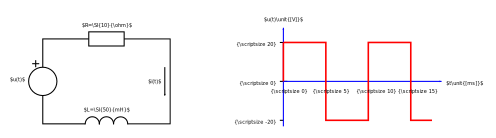
\includegraphics{Imatges/Cap-Fourier-Exemple-Circuit.pdf}
\end{figure}

 El per\'{\i}ode de la tensi\'{o} $u(t)$ \'{e}s: $T=10\unit{ms}$, i la
seva velocitat angular: $\omega = 2\pi/T = 200\pi\unit{rad/s}$;
matem\`{a}ticament, $u(t)$ s'expressa com:
\[
u(t) = \begin{cases} \rule{3.2mm}{0pt} 20\unit{V} & 0\unit{ms} < t < 5\unit{ms} \\
       -20\unit{V} & 5\unit{ms} \leq t \leq 10\unit{ms} \end{cases}
\]

Comencem calculant l'expansi\'{o} en s\`{e}rie de Fourier de la tensi\'{o}
$u(t)$. Aquesta funci\'{o} es senar i t\'{e} simetria de semiona, i per tant
 compleix: $u(t)=-u(-t)$ i $u(t) = -u(t+\frac{T}{2})$; com a
conseq\"{u}\`{e}ncia d'aix\`{o}, \'{u}nicament seran diferents de zero el
coeficients $B_n$ d'\'{\i}ndex senar $(B_1,B_3,B_5,\ldots)$. Donat que
$u(t)$ est\`{a} definida en dos trossos, calcularem els coeficients
$B_n$ segons:
\[
\begin{split}
    B_n &= \frac{2}{T} \left( \int_0^{T/2} u(t) \sin(n \omega t) +
    \int_{T/2}^{T} u(t) \sin(n \omega t) \right) =\\[0.5ex]
    &= 200 \left( \int_0^{5\cdot 10^{-3}} 20 \sin(200 n \pi t) +
    \int_{5\cdot 10^{-3}}^{10^{-2}} -20 \sin(200 n \pi t) \right) =\\[0.5ex]
    &= 200 \left( \left. -\frac{\cos(200 n \pi t)}{10 n \pi}\right|_0^{5\cdot 10^{-3}}
    +  \left.\frac{\cos(200 n \pi t)}{10 n \pi}\right|_{5\cdot
    10^{-3}}^{10^{-2}}\right)=\\[0.5ex]
    &= 200\left( \frac{1}{10 n \pi} - \frac{\cos n \pi}{5 n \pi} +
    \frac{\cos (2 n \pi)}{10 n \pi}\right)
    \qquad\qquad(n=1,3,5,\ldots)
\end{split}
\]

Si tenim en compte que per a valors senars de l'\'{\i}ndex $n$, es
compleix: $\cos n \pi = -1$ i $\cos (2 n \pi) = 1$, tenim:
\[
    B_n = 200 \left( \frac{1}{10 n \pi} - \frac{-1}{5 n \pi} +
    \frac{1}{10 n \pi} \right) = \frac{80}{n \pi}
    \qquad\qquad(n=1,3,5,\ldots)
\]

Aix\'{\i} doncs, l'expansi\'{o} en s\`{e}rie de Fourier de la tensi\'{o} $u(t)$ \'{e}s:
\[
    u(t) = \frac{80}{\pi} \left( \sin \omega t + \frac{\sin (3 \omega t)}{3} +
    \frac{\sin (5 \omega t)}{5} + \frac{\sin (7 \omega t)}{7} +
    \frac{\sin (9 \omega t)}{9} + \frac{\sin (11 \omega t)}{11} +\cdots\right)
\]

En el punt de discontinu\"{\i}tat $t=5\unit{ms}$, tenim:
\[
    u(5\cdot10^{-3}\unit{s}) =\frac{80}{\pi} \left( \sin \pi + \frac{\sin 3 \pi}{3} +
    \frac{\sin 5 \pi}{5} + \frac{\sin 7 \pi}{7} +
    \frac{\sin 9 \pi}{9} +\frac{\sin 11 \pi}{11}+\cdots\right) = 0\unit{V}
\]

Es comprova que en complir-se la condici\'{o} de Dirichlet, aquest valor
correspon al valor mitj\`{a} dels l\'{\i}mits esquerra (20) i dret (-20)  de
la funci\'{o} en aquest punt.

A continuaci\'{o} es pot veure la gr\`{a}fica de la tensi\'{o} $u(t)$, que
s'obt\'{e} utilitzant la seva expansi\'{o} en s\`{e}rie de Fourier, fins a la
component harm\`{o}nica d'\'{\i}ndex 11:
\begin{figure}[h]
\centering
    \includegraphics{Imatges/Cap-Fourier-Exemple-Tensio.pdf}
\end{figure}

La imped\`{a}ncia de la c\`{a}rrega formada per la resist\`{e}ncia $R$ i la
induct\`{a}ncia $L$, tindr\`{a} un valor $\cmplx{Z}_n$ diferent per a
cadascuna de les tensions fonamental i harm\`{o}niques presents en la
tensi\'{o} $u(t)$; els valors de $\cmplx{Z}_n$ per als primes \'{\i}ndex s\'{o}n:
\begin{alignat*}{3}
    \cmplx{Z}_1 &= R + \ju\, \omega L &&= (10 + \ju\cdot 200\cdot \pi\cdot 50\cdot 10^{-3})\unit{\ohm} &&=32{,}9691_{\measuredangle
    1{,}2626\unit{rad}}\unit{\ohm}\\
    \cmplx{Z}_3 &= R + \ju\, 3 \omega L &&= (10 + \ju\cdot 3\cdot 200\cdot \pi\cdot 50\cdot 10^{-3})\unit{\ohm} &&=94{,}7768_{\measuredangle
    1{,}4651\unit{rad}}\unit{\ohm}\\
    \cmplx{Z}_5 &= R + \ju\, 5 \omega L &&= (10 + \ju\cdot 5\cdot 200\cdot \pi\cdot 50\cdot 10^{-3})\unit{\ohm} &&=157{,}3976_{\measuredangle
    1{,}5072\unit{rad}}\unit{\ohm}\\
    \cmplx{Z}_7 &= R + \ju\, 7 \omega L &&= (10 + \ju\cdot 7\cdot 200\cdot \pi\cdot 50\cdot 10^{-3})\unit{\ohm} &&=220{,}1387_{\measuredangle
    1{,}5254\unit{rad}}\unit{\ohm}\\
    \cmplx{Z}_9 &= R + \ju\, 9 \omega L &&= (10 + \ju\cdot 9\cdot 200\cdot \pi\cdot 50\cdot 10^{-3})\unit{\ohm} &&=282{,}9201_{\measuredangle
    1{,}5354\unit{rad}}\unit{\ohm}\\
    \cmplx{Z}_{11} &= R + \ju\, 11 \omega L &&= (10 + \ju\cdot 11\cdot 200\cdot \pi\cdot 50\cdot 10^{-3})\unit{\ohm} &&=345{,}7198_{\measuredangle
    1{,}5419\unit{rad}}\unit{\ohm}
\end{alignat*}

L'expansi\'{o} en s\`{e}rie de Fourier del corrent $i(t)$ ser\`{a} an\`{a}loga a la
de la tensi\'{o} $u(t)$, \'{e}s a dir, tan sols tindr\`{a} funcions sinus
d'\'{\i}ndex senar. Donat que la c\`{a}rrega \'{e}s inductiva, cadascun dels
termes del corrent estar\`{a} endarrerit respecte del terme corresponent
de la tensi\'{o}, en un valor indicat per l'argument de cada imped\`{a}ncia.
El valor de pic de cada terme del corrent $\hat{I}_n$, s'obt\'{e}
dividint el valor de pic de cada terme de la tensi\'{o} $\hat{U}_n$ pel
m\`{o}dul de la imped\`{a}ncia corresponent; els valors de $\hat{I}_n$ per
als primes \'{\i}ndex s\'{o}n:
\begin{align*}
    \hat{I}_1 &= \frac{\hat{U}_1}{|\cmplx{Z}_1|} = \frac{80\unit{V}}{\pi\cdot32{,}9691\unit{\ohm}} = 0{,}7724\unit{A}
    & \hat{I}_3 &= \frac{\hat{U}_3}{|\cmplx{Z}_3|} =\frac{80\unit{V}}{3\cdot\pi\cdot 94{,}7768\unit{\ohm}} = 0{,}0896\unit{A}\\[0.5ex]
    \hat{I}_5 &= \frac{\hat{U}_5}{|\cmplx{Z}_5|} =\frac{80\unit{V}}{5\cdot\pi\cdot 157{,}3976\unit{\ohm}} =0{,}0324\unit{A}
    & \hat{I}_7 &= \frac{\hat{U}_7}{|\cmplx{Z}_7|} =\frac{80\unit{V}}{7\cdot\pi\cdot 220{,}1387\unit{\ohm}} =
    0{,}0165\unit{A}\\[0.5ex]
    \hat{I}_9 &= \frac{\hat{U}_9}{|\cmplx{Z}_9|} =\frac{80\unit{V}}{9\cdot\pi\cdot 282{,}9201\unit{\ohm}} =
    0{,}0100\unit{A} & \hat{I}_{11} &= \frac{\hat{U}_{11}}{|\cmplx{Z}_{11}|} =\frac{80\unit{V}}
    {11\cdot\pi\cdot 345{,}7198\unit{\ohm}} =  0{,}0067\unit{A}
\end{align*}

Amb aquests valor calculats, l'expansi\'{o} en s\`{e}rie de Fourier del
corrent $i(t)$ \'{e}s:
\[\begin{split}
     i(t) &=  0{,}7724 \sin(\omega t - 1{,}2626) +  0{,}0896 \sin(3 \omega t -
     1{,}4651) + 0{,}0324 \sin(5 \omega t - 1{,}5072) +{}\\
     &+ 0{,}0165 \sin(7 \omega t - 1{,}5254) + 0{,}0100 \sin(9 \omega t - 1{,}5354)
     +0{,}0067 \sin(11 \omega t - 1{,}5419) +\cdots
\end{split}\]

A continuaci\'{o} es pot veure la gr\`{a}fica del corrent $i(t)$, que s'obt\'{e}
utilitzant la seva expansi\'{o} en s\`{e}rie de Fourier, fins a la component
harm\`{o}nica d'\'{\i}ndex 11:

\begin{figure}[h]
\centering
  \includegraphics{Imatges/Cap-Fourier-Exemple-Corrent.pdf}
\end{figure}

Calculem a continuaci\'{o} el valor efica\c{c} $I$ del corrent:
\[\begin{split}
    I &= \sqrt{\left(\tfrac{0{,}7724}{\sqrt{2}}\unit{A}\right)^2 +
        \left(\tfrac{0{,}0896}{\sqrt{2}}\unit{A}\right)^2 +
        \left(\tfrac{0{,}0324}{\sqrt{2}}\unit{A}\right)^2 +
        \left(\tfrac{0{,}0165}{\sqrt{2}}\unit{A}\right)^2 +
        \left(\tfrac{0{,}0100}{\sqrt{2}}\unit{A}\right)^2 +
        \left(\tfrac{0{,}0067}{\sqrt{2}}\unit{A}\right)^2 \cdots}
        \,\approx \\[1ex]
        &\approx 0{,}5505\unit{A}
\end{split}\]

Finalment, la pot\`{e}ncia $P$ dissipada en la resist\`{e}ncia ser\`{a}:
\[
    P = R I^2 \approx 10\unit{\ohm} \cdot (0{,}5505\unit{A})^2 =
    3{,}03\unit{W}
\]

Aquest valor tamb\'{e} es pot calcular a partir de l'equaci\'{o}
\eqref{eq:pot_fu}. La pot\`{e}ncia aix\'{\i} calculada, correspon a la
pot\`{e}ncia activa cedida per la font de tensi\'{o}, i donat que la
resist\`{e}ncia $R$ \'{e}s l'\'{u}nic component del circuit que en consumeix,
aquest m\`{e}tode ens proporcionar\`{a} el mateix resultat; utilitzant les
expansions en s\`{e}rie de Fourier de la tensi\'{o} $u(t)$ i del corrent
$i(t)$, fins a la component harm\`{o}nica d'\'{\i}ndex 11, tenim:
\[\begin{split}
    P &\approx U_1 I_1 \cos\varphi_1 +  U_3 I_3 \cos\varphi_3 +
     U_5 I_5 \cos\varphi_5 +{}\\[0.7ex]
     &+  U_7 I_7 \cos\varphi_7 +
     U_9 I_9 \cos\varphi_9 + U_{11} I_{11} \cos\varphi_{11} ={}
\end{split}\]


\[\begin{split}
    &= \frac{80}{\pi\cdot\sqrt{2}}\unit{V} \cdot
    \frac{0{,}7724}{\sqrt{2}}\unit{A} \cdot \cos 1{,2626} +
    \frac{80}{3\cdot\pi\cdot\sqrt{2}}\unit{V} \cdot
    \frac{0{,}0896}{\sqrt{2}}\unit{A} \cdot \cos 1{,4651} + {} \\[0.7ex]
    &+ \frac{80}{5\cdot\pi\cdot\sqrt{2}}\unit{V} \cdot
    \frac{0{,}0324}{\sqrt{2}}\unit{A} \cdot \cos 1{,5072} +
    \frac{80}{7\cdot\pi\cdot\sqrt{2}}\unit{V} \cdot
    \frac{0{,}0165}{\sqrt{2}}\unit{A} \cdot \cos 1{,5254} + {}\\[0.7ex]
    &+ \frac{80}{9\cdot\pi\cdot\sqrt{2}}\unit{V} \cdot
    \frac{0{,}0100}{\sqrt{2}}\unit{A} \cdot \cos 1{,5354} +
    \frac{80}{11\cdot\pi\cdot\sqrt{2}}\unit{V} \cdot
    \frac{0{,}0067}{\sqrt{2}}\unit{A} \cdot \cos 1{,5419}= {}\\[0.7ex]
    &=3{,}03\unit{W}
\end{split}\]

En la resoluci\'{o} d'aquest exemple, hem emprat tan sols els sis
primers termes de las s\`{e}ries de Fourier de la tensi\'{o} i del corrent;
no obstant, el valor  obtingut de la pot\`{e}ncia ha de ser prou prec\'{\i}s, ja que
els valors de pic dels termes de la s\`{e}rie del corrent, disminueixen de
valor r\`{a}pidament.

Refarem a continuaci\'{o} els c\`{a}lculs utilitzant m\'{e}s termes, amb l'ajut
del programa
\textit{Mathematica}${}^\circledR$.
\index{Mathematica@\textit{Mathematica}${}^\circledR$}
Definim en primer lloc el valor de pic de cada
 terme de la tensi\'{o} i el valor del m\`{o}dul de la imped\`{a}ncia corresponent,
calculem a continuaci\'{o} els 100 primers termes del corrent de pic, i
per acabar calculem el valor efica\c{c} del corrent i la pot\`{e}ncia:
\begin{alltt}
\bfseries\small In[1]:= u[n_] = 80 / (Pi (2n-1));\\
 In[2]:= z[n_] = Abs[10 + I (2n-1) 200 Pi 50 10^-3];\\
 In[3]:= i = Table[u[n], \{n, 1, 100\}] / Table[z[n], \{n, 1, 100\}];\\
 In[4]:= Irms = Sqrt[Apply[Plus, (i/Sqrt[2])^2]] // N\\
Out[4]:= 0.550511\\
 In[5]:= P = 10 Irms^2\\
Out[5]:= 3.03063
\end{alltt}

Tamb\'{e} podem fer aquests c\`{a}lculs amb el programa
MATLAB${}^\circledR$, tal com es veu a continuaci\'{o}:
\index{MATLAB@\textit{MATLAB}${}^\circledR$}
\begin{alltt}
\bfseries\small>> u = 80./(pi*(2*[1:1:100]-1));\\
>> z = abs(10 + i*(2*[1:1:100]-1)*200*pi*50*1e-3);\\
>> i = u./z;\\
>> Irms = sqrt(sum((i./sqrt(2)).^2))\\
Irms =\\
    0.5505\\
>> P = 10*Irms^2\\
P =\\
    3.0306
\end{alltt}

 Com es pot observar, el valor de la pot\`{e}ncia obtingut amb qualsevol dels dos
 programes,
 coincideix d'una manera prou aproximada, amb el valor calculat a m\`{a}
anteriorment.
\end{exemple}

      \addtocontents{xms}{\protect\addvspace{10pt}}
\chapter{Transformada de Laplace}\label{sec:ch-laplace}
\index{transformada de Laplace}\index{Laplace, transformada de}

\section{Introducció}
La transformada de Laplace és part de l'anomenat càlcul operacional,
i s'utilitza per convertir equacions diferencials ordinàries en
equacions lineals; un cop resoltes aquestes equacions lineals, la
transformada inversa de Laplace ens proporciona la solució de
l'equació diferencial original.

\section{Definicions}\index{transformada de
Laplace!definicions}

\subsection{Transformada de Laplace}

La transformada de Laplace $\varmathscr{L}$  converteix una funció del
temps $f(t)$, definida per a $t\geq 0$, en una funció $F(s)$, on $s$
és una variable complexa:
\begin{equation}
	f(t)\,\xrightarrow{\varmathscr{L}}\,F(s), \qquad
    \varmathscr{L}\{f(t)\} = F(s) \equiv \int_0^\infty f(t) \,e^{-s t} \diff t =
    \lim_{\tau\to\infty} \int_0^\tau f(t) \,e^{-s t} \diff t \label{eq:transf_laplace}
\end{equation}

El teorema de l'existència de la transformada de Laplace estableix
que si $f(t)$ és una funció contínua a trossos en qualsevol
interval finit contingut en $t \in [0,+\infty)$, i satisfà: $|f(t)| \leq M
e^{\alpha t}$, amb $\alpha \in \mathsfb{R}$ i $M > 0$,  llavors la
funció $F(s)$ existeix i és única per a
qualsevol $\Re s > \alpha$.

\subsection{Transformada inversa de Laplace}

La transformada inversa de Laplace $\varmathscr{L}^{-1}$ s'utilitza per
obtenir la funció original $f(t)$ a partir de la funció
transformada $F(s)$:
\begin{equation}
	F(s)\,\xrightarrow{\varmathscr{L}^{-1}}\,f(t), \qquad
    \varmathscr{L}^{-1}\{F(s)\} = f(t) \equiv \frac{1}{2 \piup j }
    \int_{\gamma-j \infty}^{\gamma+j \infty} F(s)\, e^{s t} \diff s,
    \qquad t\geq 0 \label{eq:transf_inv_laplace}
\end{equation}

on $\gamma$ és un camí vertical en el pla complex, escollit de tal
manera que totes les singularitats de la funció $F(s)$ quedin a la
seva esquerra.

\subsection{Funció graó unitari i funció impuls}\index{funció!graó
unitari} \index{funció!impuls}\index{funció!de
Heaviside}\index{funció!delta de Dirac}\index{Heaviside, funció
de}\index{Dirac, funció delta
de}\index{$\epsilonup$@$\varepsilonup_\tau(t)$}\index{$\deltaup_\tau(t)$}

Aquestes dues funcions són de gran importància en el càlcul
operacional. La funció graó unitari o funció de Heaviside
$\varepsilonup_\tau(t)$ o $\varepsilonup(t-\tau)$ en l'instant de temps
$t=\tau$ es defineix com:
\begin{equation}
    \varepsilonup_\tau(t) \equiv \varepsilonup(t-\tau) = \begin{cases} 1, & t \geq \tau \\ 0, & t < \tau \end{cases}
\end{equation}

La funció impuls o funció delta de Dirac $\deltaup_\tau(t)$ o
$\deltaup(t-\tau)$ en l'instant de temps $t=\tau$, es pot definir
mitjançant l'ús de límits o d'integrals de variable complexa, però
resulta més intuïtiu definir-la a partir de les seves propietats: la
funció és nuŀla a tot arreu excepte a $t=\tau$, i és d'àrea
unitària:
\begin{subequations}
\begin{align}
    \deltaup_\tau(t) \equiv \deltaup(t-\tau) &= 0, \quad \forall t \neq \tau \\
    \int_{-\infty}^\infty \deltaup_\tau(t) \diff t &= 1
\end{align}
\end{subequations}

Algunes propietats i relacions de les funcions $\varepsilonup_\tau(t)$ i $\deltaup_\tau(t)$, on $f(t)$ és una funció qualsevol, són:
\begin{align}
   \frac{\diff}{\diff t} \varepsilonup_\tau (t) &= \deltaup_\tau(t) \\[0.5ex]
   \int_{-\infty}^\infty f(t) \deltaup_\tau (t) \diff t &= f(\tau) \\[0.5ex]
    \int_a^b \varepsilonup_\tau (t) f(t) \diff t &= \varepsilonup_\tau(t)
    \int_\tau^b f(t) \diff t, \qquad \tau \in [a, b]
\end{align}



\section{Propietats}\index{transformada de
Laplace!propietats}

La transformada de Laplace i la transformada inversa  de Laplace tenen les
propietats que s'exposen a continuació.

\subsection{Linealitat}

Si tenim: $\varmathscr{L} \{f_1(t) \} = F_1(s)$ i $\varmathscr{L}
\{f_2(t) \} = F_2(s)$, llavors:
\begin{subequations}
\begin{alignat}{2}
    \varmathscr{L} \{ a_1 f_1(t) + a_2 f_2(t) \} &= a_1 F_1(s) +
    a_2 F_2(s), &\qquad a_1,a_2 \in \mathsfb{R} \\
    \varmathscr{L}^{-1} \{ a_1 F_1(s) + a_2 F_2(s) \} &= a_1 f_1(t) +
    a_2 f_2(t), &\qquad a_1,a_2 \in \mathsfb{R}
\end{alignat}
\end{subequations}

\subsection{Canvi d'escala}

Si tenim: $\varmathscr{L} \{f(t) \} = F(s)$, llavors:
\begin{subequations}
\begin{alignat}{2}
    \varmathscr{L} \{ f(a t) \} &= \frac{F(s/a)}{a},
     &\qquad a \in \mathsfb{R}^* \\
     \varmathscr{L}^{-1} \{ F(a s) \} &= \frac{f(t/a)}{a},
     &\qquad a \in \mathsfb{R}^*
\end{alignat}
\end{subequations}

\subsection{Translació}

Si tenim: $\varmathscr{L} \{f(t) \} = F(s)$, llavors:
\begin{subequations}
\begin{alignat}{2}
    \varmathscr{L} \{ f(t - \tau) \} &= \varmathscr{L} \{ f(t - \tau)
    \varepsilonup_\tau(t) \} = e^{-s \tau} F(s), &\qquad \tau \in \mathsfb{R}_{\geq 0} \\
    \varmathscr{L}^{-1} \{ e^{-s \tau} F(s) \} &=
    f(t-\tau) \varepsilonup_\tau(t), &\qquad \tau \in \mathsfb{R}_{\geq 0}
\end{alignat}
\end{subequations}

\subsection{Esmorteïment}

Si tenim: $\varmathscr{L} \{f(t) \} = F(s)$, llavors:
\begin{subequations}
\begin{alignat}{2}
    \varmathscr{L} \{ e^{at} f(t) \} &= F(s-a),
     &\qquad a \in \mathsfb{R}\\
    \varmathscr{L}^{-1} \{ F(s-a) \} &=e^{at} f(t),
     &\qquad a \in \mathsfb{R}
\end{alignat}
\end{subequations}

\subsection{Diferenciació}

Si tenim: $\varmathscr{L} \{f(t) \} = F(s)$, on $f(t)$ és
diferenciable $n-1$ vegades en l'interval $[0,+\infty)$, 
llavors:
\begin{subequations}
\begin{align}
    \varmathscr{L} \{ f'(t) \} &= s F(s) - f(0)\\
    \varmathscr{L} \{ f''(t) \} &= s^2 F(s) - s f(0) - f'(0)\\
    \varmathscr{L} \{ f^{(n)}(t) \} &= s^n F(s) - s^{n-1} f(0) -
    s^{n-2} f'(0) - \cdots - f^{(n-1)}(0)
\end{align}
\end{subequations}

\subsection{Integració}

Si tenim: $\varmathscr{L} \{f(t) \} = F(s)$, on $f(t)$ és una
funció contínua a trossos, 
llavors:
\begin{align}
    \varmathscr{L} \left\lbrace  \int_0^t f(\tau) \diff \tau \right\rbrace  = \frac{F(s)}{s}
\end{align}

\subsection{Producte de convolució}\index{producte de convolució}

El producte de convolució «$*$» de dues funcions $f_1(t)$ i $f_2(t)$ es
defineix com:
\begin{equation}
    f_1(t) * f_2(t) \equiv \int_0^t f_1(\tau) f_2(t-\tau) \diff\tau =
    \int_0^t f_1(t-\tau) f_2(\tau) \diff\tau
\end{equation}

Si tenim: $\varmathscr{L} \{f_1(t) \} = F_1(s)$ i $\varmathscr{L}
\{f_2(t) \} = F_2(s)$, on $f_1(t)$ i $f_2(t)$ són funcions
contínues a trossos, llavors:
\begin{align}
    \varmathscr{L} \{ f_1(t) * f_2(t) \} &= F_1(s) F_2(s)\\
    \varmathscr{L}^{-1} \{ F_1(s) F_2(s) \} &= f_1(t) * f_2(t)
\end{align}

\subsection{Funció periòdica}

Sigui $f(t)$ una funció definida en l'interval $[0,T]$ i nuŀla
fora d'aquest interval, i sigui $f\ped{P}(t)$ la funció periòdica de
període $T$ que s'origina per repetició de la funció $f(t)$; si
tenim: $\varmathscr{L} \{f(t) \} = F(s)$, llavors:
\begin{equation}
   \varmathscr{L} \{f\ped{P}(t) \} = F\ped{P}(s) = \frac{F(s)}{1-e^{-sT}}
\end{equation}

\section{Taules de transformades de Laplace}

Encara que les transformades directa i inversa de Laplace es poden
obtenir amb les equacions \eqref{eq:transf_laplace} i
\eqref{eq:transf_inv_laplace} respectivament, els càlculs
involucrats poden ser força complicats; per aquest motiu és usual
disposar de taules que recullen les transformades de Laplace d'un
gran nombre de funcions.

En la taula \vref{taula:Trans-Laplace-Fun} es pot veure una relació de
transformades de Laplace de les funcions més usuals. Totes les
constants que hi apareixen són valors reals, que tant poden ser
positius com negatius llevat que s'indiqui el contrari; la variable
$\omega$ que apareix en les funcions trigonomètriques representa la
velocitat angular, amb: $\omega=2\piup f=2\piup\,/T$.

\index{transformada de Laplace!taula de funcions}
\begin{longtable}{r<{\hspace{3em}}l}
   \caption{\label{taula:Trans-Laplace-Fun} Transformades de Laplace de funcions}\\
   \toprule[1pt]
   $f(t)$ & $F(s)$\\
   \midrule
   \endfirsthead
   \caption[]{Transformades de Laplace de funcions (\emph{ve de la pàgina anterior})} \\
   \toprule[1pt]
   $f(t)$ & $F(s)$\\
   \midrule
   \endhead
   \midrule
   \multicolumn{2}{r}{\sffamily\bfseries\color{NavyBlue}(\emph{continua a la pàgina següent})}
   \endfoot
   \endlastfoot
   $\varepsilonup_\tau(t), \quad \tau \in\mathsfb{R}_{\geq 0}$  & $\dfrac{e^{-\tau s}}{s}$\\[2.2ex]
   $\deltaup_\tau(t), \quad\tau \in \mathsfb{R}_{\geq 0}$ & $e^{-\tau s}$\\[2.2ex]
   1 & $\dfrac{1}{s}$\\[2.2ex]
   $t$ &   $\dfrac{1}{s^2}$\\[2.2ex]
   $t^n, \quad n\in\mathsfb{N}^*$ &   $\dfrac{n!}{s^{n+1}}$\\[2.2ex]
   $\dfrac{t^{n-1}}{(n-1)!}, \quad n\in\mathsfb{N}^*$ & $\dfrac{1}{s^n}$\\[2.2ex]
   $t^a$ & $\dfrac{\Gamma(a+1)}{s^{a+1}}$\\[2.2ex]
   $\dfrac{1}{\sqrt{t}}$ & $\dfrac{\sqrt{\piup}}{\sqrt{s}} $\\[2.2ex]
   $\sqrt{t}$ & $\dfrac{\sqrt{\piup}}{2 s \sqrt{s}}$\\[2ex]
   $\dfrac{e^{-a t}}{\sqrt{t}}$ & $\dfrac{\sqrt{\piup}}{\sqrt{s+a}}$\\[2.2ex]
   $e^{-a t}$ & $\dfrac{1}{s+a}$\\[2.2ex]
   $a^{-b t}, \quad a\neq 0$ & $\dfrac{1}{s+b\ln a}$\\[3.5ex]
   $1- e^{-a t}$ & $\dfrac{a}{s(s+a)}$\\[3.5ex]
   $t e^{-a t}$ & $\dfrac{1}{(s+a)^2} $\\[3.5ex]
   $(1-a t)e^{-a t}$ & $\dfrac{s}{(s+a)^2} $\\[3.5ex]
   $t^2 e^{-a t}$ & $\dfrac{2}{(s+a)^3} $\\[3.5ex]
   $\dfrac{t^{n-1}e^{-at}}{(n-1)!}, \quad n\in\mathsfb{N}^*$ & $\dfrac{1}{(s+a)^n}$\\[3.5ex]
   $\dfrac{e^{-a t}-e^{-b t}}{b-a} $ & $\dfrac{1}{(s+a)(s+b)}$\\[3.5ex]
   $\dfrac{e^{-t/a}-e^{-t/b}}{a-b} $ &  $\dfrac{1}{(a s+1)(b s+1)}$\\[3.5ex]
   $\dfrac{ae^{-a t}-be^{-b t}}{a-b} $ &  $\dfrac{s}{(s+a)(s+b)}$\\[3.5ex]
   $\dfrac{ae^{-t/b}-be^{-t/a}}{a b(a-b)} $ & $\dfrac{s}{(a s+1)(b s+1)}$\\[2.5ex]
   $\dfrac{e^t}{n!}\,\dfrac{\diff^n}{\diff t^n}(t^n e^{-t}), \quad n\in\mathsfb{N}$ & $\dfrac{(s-1)^n}{s^{n+1}}$\\[3.5ex]
   $\sin \omega t$ & $\dfrac{\omega}{s^2+\omega^2}$\\[3.5ex]
   $\cos \omega t$ & $\dfrac{s}{s^2+\omega^2}$\\[3.5ex]
   $\sin(\omega t + \varphi)$ & $\dfrac{\omega\cos\varphi+s\sin\varphi}{s^2+\omega^2}$\\[3.5ex]
   $\cos(\omega t + \varphi)$ & $\dfrac{s\cos\varphi-\omega\sin\varphi}{s^2+\omega^2}$\\[3.5ex]
   $t \sin \omega t$ & $\dfrac{2 \omega s}{(s^2+\omega^2)^2}$\\[3.5ex]
   $t \cos \omega t$ & $\dfrac{s^2-\omega^2}{(s^2+\omega^2)^2}$\\[3.5ex]
   $e^{-a t} \sin \omega t$ & $\dfrac{\omega}{(s+a)^2+\omega^2}$\\[3.5ex]
   $e^{-a t} \cos \omega t$ & $\dfrac{s+a}{(s+a)^2+\omega^2}$\\[3.5ex]
   $e^{-a t} \sin (\omega t+\varphi)$ & $\dfrac{\omega\cos\varphi+(s+a)\sin\varphi}{(s+a)^2+\omega^2}$\\[3.5ex]
   $e^{-a t} \cos (\omega t+\varphi)$ & $\dfrac{(s+a)\cos\varphi-\omega\sin\varphi}{(s+a)^2+\omega^2}$\\[3.5ex]
   $\sin^2 \omega t$ & $\dfrac{2\omega^2}{s^3+4s\omega^2}$\\[3.5ex]
   $\cos^2 \omega t$ &  $\dfrac{s^2+2\omega^2}{s^3+4s\omega^2}$\\[3.5ex]
   $\dfrac{\sin(2\sqrt{\omega t})}{\sqrt{\omega}}$ & $\dfrac{\sqrt{\piup}e^{-\omega/s}}{s\sqrt{s}}$\\[3.5ex]
   $\dfrac{\cos(2\sqrt{\omega t})}{\sqrt{t}}$ & $\dfrac{\sqrt{\piup}e^{-\omega/s}}{\sqrt{s}}$\\[3.5ex]
   $\sinh a t$ & $\dfrac{a}{s^2-a^2}$\\[3.5ex]
   $\cosh a t$ & $\dfrac{s}{s^2-a^2}$\\[3.5ex]
   $\sinh^2 a t$ & $\dfrac{2a^2}{s^3-4sa^2}$\\[3.5ex]
   $\cosh^2 a t$ & $\dfrac{s^2-2a^2}{s^3-4sa^2}$\\[3.5ex]
   $t \sinh a t$ & $\dfrac{2 a s}{\left(s^2-a^2\right)^2}$\\[3.5ex]
   $t \cosh a t$ & $\dfrac{s^2+a^2}{\left(s^2-a^2\right)^2}$\\[3.5ex]
   $e^{-b t} \sinh a t$ & $ \dfrac{a}{(s+b)^2 - a^2}$\\[3.5ex]
   $e^{-b t} \cosh a t$ & $ \dfrac{s+b}{(s+b)^2 - a^2}$\\[3.5ex]
   $J_\nu(a t), \quad \nu>-1$ & $\dfrac{\left(\sqrt{s^2+a^2}-s\right)^\nu}{a^\nu \sqrt{s^2+a^2}}$\\[3.5ex]
   $I_\nu(a t), \quad \nu>-1$ & $\dfrac{\left(s-\sqrt{s^2-a^2}\right)^\nu}{a^\nu \sqrt{s^2-a^2}}$\\[3.5ex]
   $\dfrac{J_\nu(a t)}{t}, \quad \nu>0$ & $\dfrac{\left(\sqrt{s^2+a^2}-s\right)^\nu}{\nu a^\nu}$\\[2.95ex]
   $\dfrac{I_\nu(a t)}{t}, \quad \nu>0$ & $\dfrac{\left(s-\sqrt{s^2-a^2}\right)^\nu}{\nu a^\nu}$\\[1.0ex]
   \bottomrule[1pt]
\end{longtable}


En la taula \vref{taula:Trans-Laplace-Graf} es pot veure una relació de
transformades de Laplace de diverses formes d'ona usuals.

\index{transformada de Laplace!taula de formes d'ona}
\begin{longtable}{cc}
   \caption{\label{taula:Trans-Laplace-Graf} Transformades de Laplace de formes d'ona}\\
   \toprule[1pt]
   $f(t)$ & $F(s)$\\
   \midrule
   \endfirsthead
   \caption[]{Transformades de Laplace de formes d'ona (\emph{ve de la pàgina anterior})} \\
   \toprule[1pt]
   $f(t)$ & $F(s)$\\
   \midrule
   \endhead
   \midrule
   \multicolumn{2}{r}{\sffamily\bfseries\color{NavyBlue}(\emph{continua a la pàgina següent})}
   \endfoot
   \endlastfoot
   \input{Imatges/Cap-Laplace-Funcio-1.pdf_tex} & \raisebox{0.8cm}{$K\dfrac{1-e^{a s}}{s(1-e^{-\tau s})}$}\\[3.5ex]
   \input{Imatges/Cap-Laplace-Funcio-2.pdf_tex} & \raisebox{0.8cm}{$\dfrac{K}{s(1+e^{-\tau s})}$}\\[3.5ex]
   \input{Imatges/Cap-Laplace-Funcio-3.pdf_tex} & \raisebox{1.2cm}{$K\dfrac{1-e^{-\tau s}}{s(1+e^{-\tau s})} = \dfrac{K}{s}\tanh\dfrac{\tau s}{2}$}\\[3.5ex]
   \input{Imatges/Cap-Laplace-Funcio-4.pdf_tex} & \raisebox{1.2cm}{$K\dfrac{1-e^{-\tau s}}{s(e^{\tau s}+e^{-\tau s})}$}\\[3.5ex]
   \input{Imatges/Cap-Laplace-Funcio-5.pdf_tex} & \raisebox{2.5cm}{$\dfrac{K}{s(1-e^{-\tau s})} =
   K\dfrac{1+\coth(\frac{\tau s}{2})}{2 s}$}\\[3.5ex]
   \input{Imatges/Cap-Laplace-Funcio-6.pdf_tex} & \raisebox{0.8cm}{$\dfrac{e^{-\tau s}}{s^2}\tan\alpha$}\\[3.5ex]
   \input{Imatges/Cap-Laplace-Funcio-7.pdf_tex} & \raisebox{0.8cm}{$K\dfrac{-1+e^{-\tau s}+\dfrac{\tau}{a}(1-e^{-a s})}{(\tau-a)s^2(1-e^{-\tau s})}$}\\[3.5ex]
   \input{Imatges/Cap-Laplace-Funcio-8.pdf_tex} & \raisebox{0.8cm}{$K\dfrac{1-e^{-\tau s}}{\tau s^2(1+e^{-\tau s})} = \dfrac{K}{\tau s^2}\tanh\dfrac{\tau s}{2}$}\\[3.5ex]
   \input{Imatges/Cap-Laplace-Funcio-9.pdf_tex} & \raisebox{0.8cm}{$K\dfrac{e^{-2\tau s}-2e^{-\tau s}+1}{\tau s^2(1-e^{-4\tau s})}$}\\[3.5ex]
   \input{Imatges/Cap-Laplace-Funcio-10.pdf_tex} & \raisebox{1.2cm}{$2K\dfrac{1-e^{-\tau s}}{\tau s^2(1+e^{-\tau s})}-\dfrac{K}{s}$}\\[3.5ex]
   \input{Imatges/Cap-Laplace-Funcio-11.pdf_tex} & \raisebox{0.8cm}{$\dfrac{K}{\tau s^2}-\dfrac{Ke^{-\tau s}}{s(1-e^{\tau s})}$}\\[3.5ex]
   \input{Imatges/Cap-Laplace-Funcio-12.pdf_tex} & \raisebox{0.8cm}{$K\dfrac{1-(1+\tau s)e^{-\tau s}}{\tau s^2(1-e^{-2\tau s})}$}\\[3.5ex]
   \input{Imatges/Cap-Laplace-Funcio-13.pdf_tex} & \raisebox{1.2cm}{$\dfrac{K}{\tau s^2}-2K \left(\dfrac{1}{e^{-\tau s}-1}-\dfrac{1}{e^{2\tau s}-1} \right)$}\\[3.5ex]
   \input{Imatges/Cap-Laplace-Funcio-14.pdf_tex} & \raisebox{0.8cm}{$K\dfrac{\dfrac{\piup}{\tau}}{s^2+\dfrac{\piup^2}{\tau^2}}\dfrac{(1+e^{-\tau s})}{(1-e^{-\tau s})}$}\\[3.5ex]
   \input{Imatges/Cap-Laplace-Funcio-15.pdf_tex} & \raisebox{0.8cm}{$K\dfrac{\dfrac{\piup}{\tau}}{s^2+\dfrac{\piup^2}{\tau^2}}\dfrac{1}{(1-e^{-\tau s})}$}\\[2.5ex]
    \bottomrule[1pt]
\end{longtable}

	
\begin{exemple}[\CalcTransfLaplace{}]
	\addcontentsxms{\CalcTransfLaplace}
    Es tracta de calcular la transformada de Laplace dels dos
    senyals periòdics que es mostren a continuació; el primer és una
    ona triangular i el segon és la tensió sinusoidal que s'obté amb un
    rectificador d'ona completa.

    \begin{center}
        \input{Imatges/Cap-Laplace-Exemple1.pdf_tex}
    \end{center}

    Comencem amb l'ona triangular estudiant la funció $f_1(t)$ definida
    entre $t=0$ i $t=3$, i que per repetició genera la funció $f(t)$; la
    seva expressió matemàtica és:

    \[
        f_1(t) = \begin{cases}
        \phantom{-}0, & t < 0\\
        \phantom{-}3t, & 0<t<1 \\
        -\dfrac{3}{2}t +\dfrac{9}{2}, & 1 < t < 3 \\
        \phantom{-}0, & t > 3 \end{cases}
    \]

    Amb l'ajut de les funcions graó unitari en $t=0$, $t=1$ i $t=3$,
    podem definir $f_1(t)$ com:

    \[\begin{split}
        f_1(t) &= 3t (\varepsilonup_0(t) - \varepsilonup_1(t)) + \left(-\frac{3}{2}t
        +\frac{9}{2}\right) (\varepsilonup_1(t) -
        \varepsilonup_3(t))  \\
        &=
        3t\varepsilonup_0(t)-3t\varepsilonup_1(t)-\frac{3}{2}t \varepsilonup_1(t)
        +\frac{3}{2}t \varepsilonup_3(t) +\frac{9}{2} \varepsilonup_1(t)
        -\frac{9}{2} \varepsilonup_3(t)  \\
        &=3t\varepsilonup_0(t) -\frac{9}{2}(t-1)\varepsilonup_1(t) +
        \frac{3}{2}(t-3)\varepsilonup_3(t)
    \end{split}\]

    Si ens fixem en el 1r terme, veiem en la taula
    \vref{taula:Trans-Laplace-Fun} que la  transformada de $t$ és $1/s^2$.
    Els termes 2n i 3r també contenen la funció $t$, però traslladada
    en el temps un valor d'1 i 3 respectivament, per tant, si ens fixem
    en la propietat de la translació, veiem que les seves transformades
    seran també $1/s^2$ multiplicades per $e^{-s}$ i $e^{-3s}$
    respectivament. Així doncs, amb aquestes consideracions i fent
    servir la propietat de la linealitat tenim:

    \[
        F_1(s) = \frac{3}{s^2} - \frac{9 e^{-s}}{2 s^2} + \frac{3 e^{-3s}}{2
        s^2} =\frac{6-9e^{-s}+3e^{-3s}}{2s^2}
    \]

    Finalment, calculem la transformada de la funció $f(t)$ original a
    partir de la transformada de la funció $f_1(t)$, utilitzant la
    propietat de les funcions periòdiques, amb un període $T=3$:

    \[
        F(s) = \frac{F_1(s)}{1-e^{-3s}} = \frac{6-9e^{-s}+3e^{-3s}}{2s^2(1-e^{-3s}) }
    \]

    Es pot comprovar que aquest resultat és el mateix que s'obté directament de la taula \vref{taula:Trans-Laplace-Graf}, amb els valors $K=3$, $a=1$ i $\tau=3$.

    Continuem ara  amb l'ona sinusoidal estudiant la funció $u_1(t)$
    definida entre $t=0$ i $t=\tau$, i que per repetició genera la
    funció $u(t)$; la seva expressió matemàtica és (amb període $T=
    2\tau$ i velocitat angular $\omega= 2\piup\,/T  = \piup\,/\tau$):

    \[
        u_1(t) = \begin{cases} 0, & t < 0\\ \hat{U}\sin\omega t =
        \hat{U}\sin\dfrac{\piup}{\tau}t,  & 0<t<\tau \\ 0, & t > \tau \end{cases}
    \]


    Amb l'ajut de les funcions graó unitari en $t=0$ i $t=\tau$, podem
    definir $u_1(t)$ com:

    \[
        u_1(t)=\left(\hat{U}\sin\frac{\piup}{\tau}t\right)(\varepsilonup_0(t)-\varepsilonup_\tau(t))
        =\left(\hat{U}\sin\frac{\piup}{\tau}t\right)\varepsilonup_0(t) - \left(\hat{U}\sin\frac{\piup}{\tau}t\right)\varepsilonup_\tau(t)
    \]

    Pel que fa al 2n  terme, si tenim en compte la igualtat
    trigonomètrica: $-\sin \alpha = \sin(\alpha-\frac{T}{2})$, on $T$ és
    el període, tenim:

    \[
        u_1(t) = \left(\hat{U}\sin\frac{\piup}{\tau}t\right)\varepsilonup_0(t) +
        \left(\hat{U}\sin\left(\frac{\piup}{\tau}t-\tau\right)\right)\varepsilonup_\tau(t)
    \]

    El 2n terme s'ha convertit en una funció sinus, com el 1r terme,
    però traslladada en el temps un valor $\tau$; per tant, utilitzant la
    transformada de la funció sinus que apareix en la taula
    \vref{taula:Trans-Laplace-Fun}, i fent ús de la propietat de la
    translació, tenim:

    \[
        F_1(s) = \frac{\hat{U} (\piup\,/\tau)}{s^2 + (\piup\,/\tau)^2} +
        \frac{\hat{U} (\piup\,/\tau)}{s^2 + (\piup\,/\tau)^2} e^{-\tau s} =
        \frac{\hat{U} (\piup\,/\tau)}{s^2 + (\piup\,/\tau)^2} (1+e^{-\tau s})
    \]

    Per acabar, calculem la transformada de la funció $u(t)$ original a
    partir de la transformada de la funció $u_1(t)$, utilitzant la
    propietat de les funcions periòdiques, amb un període $T=\tau$:

    \[
        F(s) = \frac{F_1(s)}{1-e^{-\tau s}} =
        \frac{\hat{U} (\piup\,/\tau) }{s^2 + (\piup\,/\tau)^2}\,\frac{1+e^{-\tau s}}{1-e^{-\tau
        s}}
    \]

    Es pot comprovar que aquest resultat és el mateix que s'obté directament de la taula \vref{taula:Trans-Laplace-Graf}, amb el valor $K=\hat{U}$.
\end{exemple}

\section{Anàlisi de circuits elèctrics}\index{transformada de
Laplace!anàlisi de circuits elèctrics}\index{analisi de circuits elèctrics@anàlisi de circuits elèctrics}

La transformada de Laplace és útil en la resolució de circuits
elèctrics, quan a més del règim permanent es vol conèixer
l'evolució transitòria prèvia de les tensions i dels corrents.

Mitjançant la transformada de Laplace, les equacions diferencials
que relacionen tensions i corrents es converteixen en equacions
lineals de més fàcil resolució. Un cop calculats els valors de
tensions i corrents en el domini operacional, utilitzem la
transformada inversa de Laplace per obtenir els valors d'aquestes
tensions i corrents en el domini temporal.

Per  resoldre aquests tipus de circuits cal conèixer-ne les
condicions inicials, és a dir, els corrents de les inductàncies i
les tensions dels condensadors. Un circuit elèctric es diu que està
relaxat, quan en l'instant inicial tots els condensadors estan
descarregats i no circula corrent per cap inductància.

A tall d'exemple tenim el circuit de la figura
\vref{pic:transf-Laplace}, on en l'instant inicial $t=0$ circula un
corrent $i_0$ i el condensador $C$ està carregat a una tensió $u_0$.

\begin{center}
    \input{Imatges/Cap-Laplace-Circuit-RLC.pdf_tex}
    \captionof{figure}{Anàlisi de circuits mitjançant la transformada de Laplace}
    \label{pic:transf-Laplace}
\end{center}

Escrivim, en primer lloc,  la relació entre $u(t)$ i $i(t)$, a partir
de les relacions individuals entre tensió i corrent per a cada
component del circuit, les quals s'han exposat en la secció
\vref{sec:comp_elem}:
\begin{equation}
    u(t) = R i(t) + L \frac{\diff i(t)}{\diff t} + u_0 + \frac{1}{C}
    \int_0^t i(t) \diff t
\end{equation}

Transformem a continuació aquesta equació en una altra en el domini
operacional, essent $\varmathscr{L}\{u(t)\} = U(s)$,
$\varmathscr{L}\{i(t)\} = I(s)$ i $\varmathscr{L}\{u_0\} =
u_0/s$, i aplicant les propietats de la diferenciació i de la
integració a $i(t)$:
\begin{equation}\begin{split}
    U(s) &= R I(s) + L(s I(s) -i_0) + \frac{u_0}{s} + \frac{I(s)}{s
    C} \\[1ex]
    &= \left( R + s L +\frac{1}{s C}\right)I(s) + \frac{u_0}{s} - L i_0
\end{split}\end{equation}

De fet, aquesta equació la podríem haver escrit directament a
partir de les relacions entre les tensions i els corrents en el
domini operacional per a cada  component del circuit, les quals
s'han exposat també en la secció \vref{sec:comp_elem}.

Per tant, essent $u(t)$  una funció determinada  ---sinusoidal, impuls,
graó, etc.--- podem obtenir $U(s)$ i calcular $I(s)$ mitjançant:
\begin{equation}
    I(s) = \frac{U(s)-\dfrac{u_0}{s} + L i_0}{R + s L
    +\dfrac{1}{s C}}\label{eq:i-Laplace}
\end{equation}

Finalment, obtenim el corrent en el domini temporal: $i(t) =
\varmathscr{L}^{-1}\{I(s)\}$.

	
\begin{exemple}[\ResCircRC{}]
	\addcontentsxms{\ResCircRC}
    A partir del circuit de la figura \vref{pic:transf-Laplace}, amb
    $L=0$, $i_0=0$ i $u_0=0$, es tracta de calcular el corrent $i(t)$,
    essent $u(t)=U$ (valor constant).

    Comencem per escriure l'equació \eqref{eq:i-Laplace} en el nostre
    cas particular, tenint en compte que $\varmathscr{L}\{U\} = U/s$
    \[
        I(s) = \frac{U}{s\left(R + \dfrac{1}{s C}\right)} = \frac{C U}{1 + s R C}
    \]

    A continuació, dividim numerador i denominador per $R C$ per tal
    d'obtenir una expressió que es trobi en la taula
    \vref{taula:Trans-Laplace-Fun}:

    \[
        I(s) = \frac{\dfrac{U}{R}}{\dfrac{1}{R C} + s}
    \]

    Utilitzant la taula \vref{taula:Trans-Laplace-Fun}, obtenim la transformada inversa de Laplace de $I(s)$:

    \[
        i(t) = \frac{U}{R} e^{-\frac{1}{R C}t}
    \]

    Es pot veure que aquest resultat coincideix amb l'equació \eqref{eq:RC-carrega} de la secció \vref{sec:RC-carrega}.
\end{exemple}

\section{Fraccions parcials}\index{fraccions parcials}
\index{transformada de Laplace!fraccions parcials}

En l'exemple anterior, la funció de variable $s$ que hem hagut de
buscar en la taula \vref{taula:Trans-Laplace-Fun} era força simple, i, per tant, la seva transformada inversa s'ha obtingut de forma
immediata. Tanmateix, és més usual tenir funcions racionals ---quocient de dos polinomis--- de grau elevat; en aquest cas cal
descompondre aquesta funció racional en suma de funcions parcials de
grau menor.

S'exposa a continuació la teoria de la descomposició en fraccions
parcials.

Sigui $\frac{P(x)}{Q(x)}$ una funció racional, on el grau de $P(x)$
és menor que el de $Q(x)$ i el coeficient del terme de grau més
elevat de $Q(x)$ val 1. Si $Q(x)$ té $n$ arrels reals sense
multiplicitat: $a_1,\ldots,a_n$, $k$ arrels reals: $b_1,\ldots,b_k$
cadascuna amb la seva multiplicitat: $m_1,\ldots,m_k$, i $l$ arrels
complexes conjugades sense multiplicitat: $c_1\pm
j\,d_1,\ldots,c_l\pm j\,d_l$, aquest polinomi es pot escriure
com el producte següent:

\begin{equation}
    Q(x)= (x-a_1) \cdots (x-a_n)(x-b_1)^{m_1} \cdots (x-b_k)^{m_k}
    ((x-c_1)^2+d_1^2)\cdots((x-c_l)^2+d_l^2)
\end{equation}

Les arrels $a_i$ són, de fet, un cas particular de les arrels $b_i$,
amb multiplicitat 1.

A parir de les arrels de $Q(x)$, la funció  racional
$\frac{P(x)}{Q(x)}$ es pot expressar com:

\begin{equation}\begin{split}
    \frac{P(x)}{Q(x)} &= \frac{A_1}{x-a_1} + \frac{A_2}{x-a_2}
    + \cdots + \frac{A_n}{x-a_n}  \\[1.5ex]
   &+ \frac{B_{1,1}}{(x-b_1)^{m_1}} + \frac{B_{1,2}}{(x-b_1)^{m_1-1}}
   + \frac{B_{1,3}}{(x-b_1)^{m_1-2}} + \cdots +
   \frac{B_{1,m_1}}{x-b_1} \\[1.5ex]
&+ \frac{B_{2,1}}{(x-b_2)^{m_2}} + \frac{B_{2,2}}{(x-b_2)^{m_2-1}}
   + \frac{B_{2,3}}{(x-b_2)^{m_2-2}} + \cdots  +
   \frac{B_{2,m_2}}{x-b_2} \\[1.5ex]
   &+ \cdots \\[1ex]
&+ \frac{B_{k,1}}{(x-b_k)^{m_k}} + \frac{B_{k,2}}{(x-b_k)^{m_k-1}}
   + \frac{B_{k,3}}{(x-b_k)^{m_k-2}} + \cdots +
   \frac{B_{k,m_k}}{x-b_k}\\[1.5ex]
&+ \frac{C_1(x-c_1)+D_1 d_1}{(x-c_1)^2+d_1^2}+ \frac{C_2(x-c_2)+D_2
d_2}{(x-c_2)^2+d_2^2} +  \cdots +\frac{C_l(x-c_l)+D_l d_l}{(x-c_l)^2+d_l^2}\\[1.5ex]
\end{split}\end{equation}

Els coeficients $A_i$, $B_{i,j}$, $C_i$ i $D_i$ es calculen a
partir de les equacions següents:
\begin{subequations}
\begin{alignat}{2}
     &A_i = \left. (x-a_i)\frac{P(x)}{Q(x)} \right|_{x=a_i},
     &\qquad i=1,\ldots,n\\[1.5ex]
     &B_{i,j} = \left. (x-b_i)^{m_i} \frac{P(x)}{Q(x)}\right|_{x=b_i},
     &\qquad i=1,\ldots,k, \quad j=1 \\[1.5ex]
    &B_{i,j} = \left. \frac{1}{(j-1)!} \; \frac{\diff^{j-1}}{\diff
    x^{j-1}} \left[ (x-b_i)^{m_i} \frac{P(x)}{Q(x)}\right]\right|_{x=b_i},
     &\qquad i=1,\ldots,k, \quad j=2,\ldots,m_i\\[1.5ex]
   &D_i+j\, C_i  =  \left.\frac{1}{d_i} ((x-c_i)^2+d_i^2) \frac{P(x)}{Q(x)}
    \right|_{x=c_i+j\,d_i}, &\qquad i=1,\ldots,l
\end{alignat}
\end{subequations}


\begin{exemple}[\CircuitLaplace{} \hyperlink{exemple:CircuitLaplace}{\large\textcolor{NavyBlue}{(\faPython)}}]\label{ex:CircuitLaplace}
	\addcontentsxms{\CircuitLaplace}
    El circuit de la figura de la pàgina següent es troba en règim estacionari. En
    l'instant $t=0$ obrim l'interruptor $\mathscr{M}$; es tracta de trobar
    l'evolució del corrent $i\ped{L}(t)$, que circula per la inductància
    $L$, a partir d'aquest instant.

      Atès que abans d'obrir l'interruptor $\mathscr{M}$ el circuit ha arribat al
     règim estacionari, el condensador $C$ estarà totalment carregat  i
     presentarà una impedància infinita al corrent continu originat per la
     bateria, i la inductància $L$ hi presentarà una impedància nuŀla;
     per tant, en l'instant $t=0$ els valors inicials $i\ped{L}(0)$ i
     $u\ped{C}(0)$ són:
     \begin{align*}
        i\ped{L}(0) &= \frac{U\ped{bat}}{R\ped{bat} + R_3} = \frac{\qty{120}{V}}
        {\qty{5}{\ohm} + \qty{25}{\ohm}} = \qty{4}{A} \\[0.5ex]
        u\ped{C}(0) &= i\ped{L}(0) R_3 = \qty{4}{A}\times \qty{25}{\ohm} = \qty{100}{V}
     \end{align*}

  \begin{center}
	\input{Imatges/Cap-Laplace-Exemple3-Circuit.pdf_tex}
\end{center}

    Un cop obrim l'interruptor $\mathscr{M}$, la bateria i la seva resistència
    queden desconnectades de les dues malles de la part dreta del circuit; si apliquem la llei de les tensions de Kirchhoff  a aquestes
    dues malles, utilitzant les variables $I\ped{L}(s)$, $U\ped{C}(s)$ i
    $I\ped{C}(s)$, tenim:
    \begin{align*}
        R_1 I\ped{L}(s) + s L I\ped{L}(s) - L i\ped{L}(0) + R_2
        (I\ped{L}(s) + I\ped{C}(s)) &=0 \\[0.5ex]
        U\ped{C}(s) + R_3 I\ped{C}(s) + R_2 (I\ped{L}(s) + I\ped{C}(s)) &=0
    \end{align*}

    La relació entre $U\ped{C}(s)$ i $I\ped{C}(s)$ és:
    \begin{equation*}
        U\ped{C}(s) = \frac{I\ped{C}(s)}{s C} + \frac{u\ped{C}(0)}{s}
        \quad\Rightarrow\quad I\ped{C}(s) = s C U\ped{C}(s) - C u\ped{C}(0)
    \end{equation*}

    Si substituïm aquest valor de $I\ped{C}(s)$ en les dues equacions
    inicials i en reordenem els termes, obtenim les dues equacions següents:
    \begin{align*}
        R_1 I\ped{L}(s) + s L I\ped{L}(s)  + R_2
        I\ped{L}(s) + s C R_2 U\ped{C}(s) &= L i\ped{L}(0) + C R_2 u\ped{C}(0)\\[0.5ex]
        U\ped{C}(s) + s C R_3 U\ped{C}(s) + R_2 I\ped{L}(s) + s C R_2 U\ped{C}(s)
        &= C R_3 u\ped{C}(0) + C R_2 u\ped{C}(0)
    \end{align*}

    Agrupem a continuació els termes comuns i substituïm $u\ped{C}(0)$ i
    $i\ped{L}(0)$ pels seus valor numèrics:
    \begin{align*}
        (R_1 + s L + R_2) I\ped{L}(s) + s C R_2 U\ped{C}(s) &= 4 L  + 100 C R_2\\[0.5ex]
        R_2 I\ped{L}(s) + (1 +s C R_3 + s C R_2) U\ped{C}(s) &= 100 C R_3  + 100 C R_2
    \end{align*}

    Aïllem ara $U\ped{C}(s)$ en la primera equació:
    \[
        U\ped{C}(s) = \frac{4 L  + 100 C R_2 -(R_1 + s L + R_2) I\ped{L}(s)}{s C R_2}
    \]

    Substituïm tot seguit aquest valor en la segona equació i aïllem
    $I\ped{L}(s)$:
    \begin{gather*}
       R_2 I\ped{L}(s) + (1 + s C R_3 + s C R_2) \frac{4 L  + 100 C R_2 - (R_1 + s L + R_2)I\ped{L}(s)}{s C R_2} = 100 C R_3  + 100 C R_2 \\[1.5ex]
       \begin{split} &\left( R_2 - \frac{(1 +s C R_3 + s C R_2)(R_1 + s L + R_2)}{s C R_2} \right) I\ped{L}(s)
        \\[1ex] &= 100 C (R_3  + R_2) - \frac{(1 +s C R_3 + s C R_2)(4 L  + 100 C R_2)}{s C
       R_2}\end{split}\\[1.5ex]
    I\ped{L}(s) = \frac{100 s C^2 R_2(R_3  + R_2)- (1 +s C R_3 + s C
    R_2)(4 L  + 100 C R_2)}{s C R_2^2  -(1 +s C R_3 + s C R_2)(R_1 + s L
    + R_2)}
    \end{gather*}

    Si donem valors numèrics a $R_1$, $R_2$, $R_3$, $L$ i $C$, i
    realitzem tots els productes i les  simplificacions oportunes,
    obtenim:
    \[
    I\ped{L}(s) = \frac{4 s+ 4300}{s^2 +1475 s + 700000}
    \]

    Hem de descompondre a continuació aquesta funció racional en
    funcions parcials; comencem doncs per calcular les arrels del
    polinomi del denominador:
    \[
    s^2 +1475 s + 700000 = 0 \quad\Rightarrow\quad s= -\frac{1475}{2}
    \pm j\,\frac{75\sqrt{111}}{2}
    \]

    A partir d'aquests valors, la  funció racional es pot escriure com:
    \[
        I\ped{L}(s) =
        \frac{4 s+ 4300}{s^2 +1475 s + 700000} =
        \frac{C\left(s+\dfrac{1475}{2}\right)+D\dfrac{75\sqrt{111}}{2}}
        {\left(s+\dfrac{1475}{2}\right)^2+\left(\dfrac{75\sqrt{111}}{2}\right)^2}
    \]

    Les constants $C$ i $D$ valen:
    \[
    D + j\,C = \left.\frac{2}{75\sqrt{111}}(4 s
    +4300)\right|_{s=-\frac{1475}{2} + j\,\frac{75\sqrt{111}}{2}}=
    12\sqrt{\frac{3}{37}} +j\,4
    \]

    Així doncs, amb $C=4$ i $D=12\sqrt{\frac{3}{37}}$, podem expressar
    el corrent $I\ped{L}(s)$ com:
    \[
        I\ped{L}(s) = 4\times\frac{s+\dfrac{1475}{2}}
        {\left(s+\dfrac{1475}{2}\right)^2+\left(\dfrac{75\sqrt{111}}{2}\right)^2}
        + 12\sqrt{\frac{3}{37}}\times\frac{\dfrac{75\sqrt{111}}{2}}
        {\left(s+\dfrac{1475}{2}\right)^2+\left(\dfrac{75\sqrt{111}}{2}\right)^2}
    \]


     Si ens fixem ara en la taula \vref{taula:Trans-Laplace-Fun},
    veiem que la transformada inversa de Laplace del primer terme de
    $I\ped{L}(s)$, es pot identificar amb una funció del tipus
    $e^{-at}\cos\omega t$, i la del segon terme amb una funció del tipus
    $e^{-at}\sin\omega t$, amb $a=\frac{1475}{2}$ i
    $\omega=\frac{75\sqrt{111}}{2}$.

    Per tant, l'expressió temporal del corrent $i\ped{L}(t)$ és:
    \[\begin{split}
        i\ped{L}(t) &= 4\, e^{-\frac{1475}{2}t} \cos \frac{75\sqrt{111}}{2} t +
        12\sqrt{\frac{3}{37}}\, e^{-\frac{1475}{2}t} \sin
        \frac{75\sqrt{111}}{2}t  \\[1ex] &= e^{-\frac{1475}{2}t} \left( 4
        \cos \frac{75\sqrt{111}}{2} t + 12\sqrt{\frac{3}{37}}\sin
        \frac{75\sqrt{111}}{2}t\right)
    \end{split}\]

    Finalment, si utilitzem la igualtat trigonomètrica
    \eqref{eq:AcosBsin}, tenim:
    \[
    i\ped{L}(t) = \frac{32}{\sqrt{37}}\,e^{-\frac{1475}{2}t}
    \cos\left(\frac{75\sqrt{111}}{2} t - \arctan
    \sqrt{\frac{27}{37}}\right)
    \]

    Si en aquesta equació fem $t=0$, tenim:
    \[
        i\ped{L}(0) = \frac{32}{\sqrt{37}} \cos\left( - \arctan
    \sqrt{\frac{27}{37}}\right) = \qty{4}{A}
    \]

    Es comprova que aquest valor compleix amb la condició inicial del
    corrent $i\ped{L}(t)$ que hem calculat a l'inici d'aquest exemple.

    Representem a continuació la gràfica d'aquesta funció:

    \begin{center}
        % GNUPLOT: LaTeX picture with Postscript
\begingroup
  \makeatletter
  \providecommand\color[2][]{%
    \GenericError{(gnuplot) \space\space\space\@spaces}{%
      Package color not loaded in conjunction with
      terminal option `colourtext'%
    }{See the gnuplot documentation for explanation.%
    }{Either use 'blacktext' in gnuplot or load the package
      color.sty in LaTeX.}%
    \renewcommand\color[2][]{}%
  }%
  \providecommand\includegraphics[2][]{%
    \GenericError{(gnuplot) \space\space\space\@spaces}{%
      Package graphicx or graphics not loaded%
    }{See the gnuplot documentation for explanation.%
    }{The gnuplot epslatex terminal needs graphicx.sty or graphics.sty.}%
    \renewcommand\includegraphics[2][]{}%
  }%
  \providecommand\rotatebox[2]{#2}%
  \@ifundefined{ifGPcolor}{%
    \newif\ifGPcolor
    \GPcolortrue
  }{}%
  \@ifundefined{ifGPblacktext}{%
    \newif\ifGPblacktext
    \GPblacktexttrue
  }{}%
  % define a \g@addto@macro without @ in the name:
  \let\gplgaddtomacro\g@addto@macro
  % define empty templates for all commands taking text:
  \gdef\gplbacktext{}%
  \gdef\gplfronttext{}%
  \makeatother
  \ifGPblacktext
    % no textcolor at all
    \def\colorrgb#1{}%
    \def\colorgray#1{}%
  \else
    % gray or color?
    \ifGPcolor
      \def\colorrgb#1{\color[rgb]{#1}}%
      \def\colorgray#1{\color[gray]{#1}}%
      \expandafter\def\csname LTw\endcsname{\color{white}}%
      \expandafter\def\csname LTb\endcsname{\color{black}}%
      \expandafter\def\csname LTa\endcsname{\color{black}}%
      \expandafter\def\csname LT0\endcsname{\color[rgb]{1,0,0}}%
      \expandafter\def\csname LT1\endcsname{\color[rgb]{0,1,0}}%
      \expandafter\def\csname LT2\endcsname{\color[rgb]{0,0,1}}%
      \expandafter\def\csname LT3\endcsname{\color[rgb]{1,0,1}}%
      \expandafter\def\csname LT4\endcsname{\color[rgb]{0,1,1}}%
      \expandafter\def\csname LT5\endcsname{\color[rgb]{1,1,0}}%
      \expandafter\def\csname LT6\endcsname{\color[rgb]{0,0,0}}%
      \expandafter\def\csname LT7\endcsname{\color[rgb]{1,0.3,0}}%
      \expandafter\def\csname LT8\endcsname{\color[rgb]{0.5,0.5,0.5}}%
    \else
      % gray
      \def\colorrgb#1{\color{black}}%
      \def\colorgray#1{\color[gray]{#1}}%
      \expandafter\def\csname LTw\endcsname{\color{white}}%
      \expandafter\def\csname LTb\endcsname{\color{black}}%
      \expandafter\def\csname LTa\endcsname{\color{black}}%
      \expandafter\def\csname LT0\endcsname{\color{black}}%
      \expandafter\def\csname LT1\endcsname{\color{black}}%
      \expandafter\def\csname LT2\endcsname{\color{black}}%
      \expandafter\def\csname LT3\endcsname{\color{black}}%
      \expandafter\def\csname LT4\endcsname{\color{black}}%
      \expandafter\def\csname LT5\endcsname{\color{black}}%
      \expandafter\def\csname LT6\endcsname{\color{black}}%
      \expandafter\def\csname LT7\endcsname{\color{black}}%
      \expandafter\def\csname LT8\endcsname{\color{black}}%
    \fi
  \fi
    \setlength{\unitlength}{0.0500bp}%
    \ifx\gptboxheight\undefined%
      \newlength{\gptboxheight}%
      \newlength{\gptboxwidth}%
      \newsavebox{\gptboxtext}%
    \fi%
    \setlength{\fboxrule}{0.5pt}%
    \setlength{\fboxsep}{1pt}%
\begin{picture}(8220.00,4800.00)%
    \gplgaddtomacro\gplbacktext{%
      \colorrgb{0.00,0.00,0.00}%%
      \put(558,787){\makebox(0,0)[r]{\strut{}-1}}%
      \colorrgb{0.00,0.00,0.00}%%
      \put(558,1546){\makebox(0,0)[r]{\strut{} 0}}%
      \colorrgb{0.00,0.00,0.00}%%
      \put(558,2304){\makebox(0,0)[r]{\strut{} 1}}%
      \colorrgb{0.00,0.00,0.00}%%
      \put(558,3063){\makebox(0,0)[r]{\strut{} 2}}%
      \colorrgb{0.00,0.00,0.00}%%
      \put(558,3821){\makebox(0,0)[r]{\strut{} 3}}%
      \colorrgb{0.00,0.00,0.00}%%
      \put(558,4580){\makebox(0,0)[r]{\strut{} 4}}%
      \colorrgb{0.00,0.00,0.00}%%
      \put(742,481){\makebox(0,0){\strut{}$0$}}%
      \colorrgb{0.00,0.00,0.00}%%
      \put(1450,481){\makebox(0,0){\strut{}$1$}}%
      \colorrgb{0.00,0.00,0.00}%%
      \put(2157,481){\makebox(0,0){\strut{}$2$}}%
      \colorrgb{0.00,0.00,0.00}%%
      \put(2865,481){\makebox(0,0){\strut{}$3$}}%
      \colorrgb{0.00,0.00,0.00}%%
      \put(3573,481){\makebox(0,0){\strut{}$4$}}%
      \colorrgb{0.00,0.00,0.00}%%
      \put(4281,481){\makebox(0,0){\strut{}$5$}}%
      \colorrgb{0.00,0.00,0.00}%%
      \put(4988,481){\makebox(0,0){\strut{}$6$}}%
      \colorrgb{0.00,0.00,0.00}%%
      \put(5696,481){\makebox(0,0){\strut{}$7$}}%
      \colorrgb{0.00,0.00,0.00}%%
      \put(6404,481){\makebox(0,0){\strut{}$8$}}%
      \colorrgb{0.00,0.00,0.00}%%
      \put(7111,481){\makebox(0,0){\strut{}$9$}}%
      \colorrgb{0.00,0.00,0.00}%%
      \put(7819,481){\makebox(0,0){\strut{}$10$}}%
    }%
    \gplgaddtomacro\gplfronttext{%
      \csname LTb\endcsname%%
      \put(255,2683){\rotatebox{-270}{\makebox(0,0){\strut{}$i\ped{L}(t)\, / \,\unit{A}$}}}%
      \csname LTb\endcsname%%
      \put(7873,2683){\rotatebox{-270}{\makebox(0,0){\strut{}}}}%
      \csname LTb\endcsname%%
      \put(4280,153){\makebox(0,0){\strut{}$t\, / \,\unit{ms}$}}%
      \csname LTb\endcsname%%
      \put(4280,4471){\makebox(0,0){\strut{}}}%
      \csname LTb\endcsname%%
      \put(4280,4580){\makebox(0,0){\strut{}}}%
    }%
    \gplbacktext
    \put(0,0){\includegraphics{Cap-Laplace-Exemple3-Corrent}}%
    \gplfronttext
  \end{picture}%
\endgroup

    \end{center}
\end{exemple}

\break	
\begin{exemple}[\CircuitLaplaceNul{}
\hyperlink{exemple:CircuitLaplaceNul}{\large\textcolor{NavyBlue}{(\faPython)}}]\label{ex:CircuitLaplaceNul}	
	\addcontentsxms{\CircuitLaplaceNul}
    El circuit de la figura següent està relaxat. En l'instant $t=0$
    tanquem l'interruptor $\mathscr{M}$; es tracta de trobar l'evolució de la tensió
    $u\ped{C}(t)$ a partir d'aquest instant.

    \begin{center}
        \input{Imatges/Cap-Laplace-Exemple4-Circuit.pdf_tex}
    \end{center}

    La transformada de Laplace de la tensió $u(t)$ és:
    \[
        U(s) = \sqrt{2}\times 220\times \frac{s}{s^2 + (100\piup)^2}
    \]

    Un cop tancat l'interruptor $\mathscr{M}$, la relació entre $u\ped{c}(t)$ i
    $u(t)$ en el domini operacional, tenint en compte que totes les
    condicions inicials són nuŀles, és:
    \[
        U\ped{C}(s) = \frac{\dfrac{1}{sC}}{R+ sL +\dfrac{1}{sC}} U(s)=
        \frac{\dfrac{1}{CL}}{s^2 + \dfrac{R}{L}s +\dfrac{1}{CL}} U(s)
    \]

    Substituint $U(s)$ per la seva expressió i donant valors numèrics a
    $R$, $L$ i $C$, tenim:
    \[
        U\ped{C}(s) = \frac{\sqrt{2}\times 110\times 10^6 s}{(s^2 + 1000 s + 500000)(s^2 + (100\piup)^2)}
    \]

    Calculem a continuació les arrels dels dos polinomis  del
    denominador d'aquesta funció racional:
    \begin{align*}
        s^2 + 1000 s + 500000 &= 0 \quad\Rightarrow\quad s = -500
        \pm j\,500 \\[0.5ex]
        s^2 + (100\piup)^2 &= 0 \quad\Rightarrow\quad s = \pm j\,100\piup
    \end{align*}

    Així doncs, l'esmentada funció racional es pot escriure com:
    \[\begin{split}
    U\ped{C}(s) &= \frac{\sqrt{2}\times 110\times 10^6 s}{(s^2 + 1000 s +
    500000)(s^2 + (100\piup)^2)}   \\[2ex] &= \frac{C_1 (s+500) + D_1
    500}{(s+500)^2+500^2} + \frac{C_2 s + D_2 100 \piup}{s^2 +(100\piup)^2}
    \end{split}\]

    Les constants $C_1$, $D_1$,  $C_2$ i $D_2$ valen:
    \begin{alignat*}{2}
        D_1 + j\,C_1 &= \left.\frac{1}{500}\times \frac{\sqrt{2}\times 110\times 10^6 s}
        {s^2 +(100\piup)^2}\right|_{s=\complexnum{-500+j500}} &&= \complexnum{-358,57 -j 240,35}\\[3.5ex]
        D_2 + j\,C_2 &= \left.\frac{1}{100\piup}\times\frac{\sqrt{2}\times 110\times 10^6 s}
        {s^2 + 1000 s + 500000}\right|_{s=j 100\piup} &&= \complexnum{188,16 + j240,35}
    \end{alignat*}

    A partir d'aquests valors i utilitzant la taula
    \vref{taula:Trans-Laplace-Fun}, obtenim l'expressió temporal de la
    tensió en el condensador $u\ped{C}(t)$:
    \[
        u\ped{C}(t) = e^{-500t} (\num{-240,35} \cos 500 t - \num{358,57} \sin 500
        t) + \num{240,35} \cos (100\piup t) + \num{188,16} \sin( 100\piup
        t)
    \]

    Utilitzant la igualtat trigonomètrica \eqref{eq:AcosBsin} obtenim finalment:
    \[
        u\ped{C}(t)= \num{431,67} e^{-500t} \cos(500 t +\num{2,1613}) + \num{305,24} \cos (100\piup t - \num{0,6642})
    \]

    Representem a continuació la gràfica d'aquesta
    funció:

    \begin{center}
      % GNUPLOT: LaTeX picture with Postscript
\begingroup
  \makeatletter
  \providecommand\color[2][]{%
    \GenericError{(gnuplot) \space\space\space\@spaces}{%
      Package color not loaded in conjunction with
      terminal option `colourtext'%
    }{See the gnuplot documentation for explanation.%
    }{Either use 'blacktext' in gnuplot or load the package
      color.sty in LaTeX.}%
    \renewcommand\color[2][]{}%
  }%
  \providecommand\includegraphics[2][]{%
    \GenericError{(gnuplot) \space\space\space\@spaces}{%
      Package graphicx or graphics not loaded%
    }{See the gnuplot documentation for explanation.%
    }{The gnuplot epslatex terminal needs graphicx.sty or graphics.sty.}%
    \renewcommand\includegraphics[2][]{}%
  }%
  \providecommand\rotatebox[2]{#2}%
  \@ifundefined{ifGPcolor}{%
    \newif\ifGPcolor
    \GPcolortrue
  }{}%
  \@ifundefined{ifGPblacktext}{%
    \newif\ifGPblacktext
    \GPblacktexttrue
  }{}%
  % define a \g@addto@macro without @ in the name:
  \let\gplgaddtomacro\g@addto@macro
  % define empty templates for all commands taking text:
  \gdef\gplbacktext{}%
  \gdef\gplfronttext{}%
  \makeatother
  \ifGPblacktext
    % no textcolor at all
    \def\colorrgb#1{}%
    \def\colorgray#1{}%
  \else
    % gray or color?
    \ifGPcolor
      \def\colorrgb#1{\color[rgb]{#1}}%
      \def\colorgray#1{\color[gray]{#1}}%
      \expandafter\def\csname LTw\endcsname{\color{white}}%
      \expandafter\def\csname LTb\endcsname{\color{black}}%
      \expandafter\def\csname LTa\endcsname{\color{black}}%
      \expandafter\def\csname LT0\endcsname{\color[rgb]{1,0,0}}%
      \expandafter\def\csname LT1\endcsname{\color[rgb]{0,1,0}}%
      \expandafter\def\csname LT2\endcsname{\color[rgb]{0,0,1}}%
      \expandafter\def\csname LT3\endcsname{\color[rgb]{1,0,1}}%
      \expandafter\def\csname LT4\endcsname{\color[rgb]{0,1,1}}%
      \expandafter\def\csname LT5\endcsname{\color[rgb]{1,1,0}}%
      \expandafter\def\csname LT6\endcsname{\color[rgb]{0,0,0}}%
      \expandafter\def\csname LT7\endcsname{\color[rgb]{1,0.3,0}}%
      \expandafter\def\csname LT8\endcsname{\color[rgb]{0.5,0.5,0.5}}%
    \else
      % gray
      \def\colorrgb#1{\color{black}}%
      \def\colorgray#1{\color[gray]{#1}}%
      \expandafter\def\csname LTw\endcsname{\color{white}}%
      \expandafter\def\csname LTb\endcsname{\color{black}}%
      \expandafter\def\csname LTa\endcsname{\color{black}}%
      \expandafter\def\csname LT0\endcsname{\color{black}}%
      \expandafter\def\csname LT1\endcsname{\color{black}}%
      \expandafter\def\csname LT2\endcsname{\color{black}}%
      \expandafter\def\csname LT3\endcsname{\color{black}}%
      \expandafter\def\csname LT4\endcsname{\color{black}}%
      \expandafter\def\csname LT5\endcsname{\color{black}}%
      \expandafter\def\csname LT6\endcsname{\color{black}}%
      \expandafter\def\csname LT7\endcsname{\color{black}}%
      \expandafter\def\csname LT8\endcsname{\color{black}}%
    \fi
  \fi
    \setlength{\unitlength}{0.0500bp}%
    \ifx\gptboxheight\undefined%
      \newlength{\gptboxheight}%
      \newlength{\gptboxwidth}%
      \newsavebox{\gptboxtext}%
    \fi%
    \setlength{\fboxrule}{0.5pt}%
    \setlength{\fboxsep}{1pt}%
\begin{picture}(8500.00,5380.00)%
    \gplgaddtomacro\gplbacktext{%
      \colorrgb{0.00,0.00,0.00}%%
      \put(752,787){\makebox(0,0)[r]{\strut{}-400}}%
      \colorrgb{0.00,0.00,0.00}%%
      \put(752,1334){\makebox(0,0)[r]{\strut{}-300}}%
      \colorrgb{0.00,0.00,0.00}%%
      \put(752,1880){\makebox(0,0)[r]{\strut{}-200}}%
      \colorrgb{0.00,0.00,0.00}%%
      \put(752,2427){\makebox(0,0)[r]{\strut{}-100}}%
      \colorrgb{0.00,0.00,0.00}%%
      \put(752,2974){\makebox(0,0)[r]{\strut{} 0}}%
      \colorrgb{0.00,0.00,0.00}%%
      \put(752,3520){\makebox(0,0)[r]{\strut{} 100}}%
      \colorrgb{0.00,0.00,0.00}%%
      \put(752,4067){\makebox(0,0)[r]{\strut{} 200}}%
      \colorrgb{0.00,0.00,0.00}%%
      \put(752,4613){\makebox(0,0)[r]{\strut{} 300}}%
      \colorrgb{0.00,0.00,0.00}%%
      \put(752,5160){\makebox(0,0)[r]{\strut{} 400}}%
      \colorrgb{0.00,0.00,0.00}%%
      \put(936,481){\makebox(0,0){\strut{}$0$}}%
      \colorrgb{0.00,0.00,0.00}%%
      \put(1652,481){\makebox(0,0){\strut{}$5$}}%
      \colorrgb{0.00,0.00,0.00}%%
      \put(2369,481){\makebox(0,0){\strut{}$10$}}%
      \colorrgb{0.00,0.00,0.00}%%
      \put(3085,481){\makebox(0,0){\strut{}$15$}}%
      \colorrgb{0.00,0.00,0.00}%%
      \put(3801,481){\makebox(0,0){\strut{}$20$}}%
      \colorrgb{0.00,0.00,0.00}%%
      \put(4518,481){\makebox(0,0){\strut{}$25$}}%
      \colorrgb{0.00,0.00,0.00}%%
      \put(5234,481){\makebox(0,0){\strut{}$30$}}%
      \colorrgb{0.00,0.00,0.00}%%
      \put(5950,481){\makebox(0,0){\strut{}$35$}}%
      \colorrgb{0.00,0.00,0.00}%%
      \put(6666,481){\makebox(0,0){\strut{}$40$}}%
      \colorrgb{0.00,0.00,0.00}%%
      \put(7383,481){\makebox(0,0){\strut{}$45$}}%
      \colorrgb{0.00,0.00,0.00}%%
      \put(8099,481){\makebox(0,0){\strut{}$50$}}%
    }%
    \gplgaddtomacro\gplfronttext{%
      \csname LTb\endcsname%%
      \put(61,2973){\rotatebox{-270}{\makebox(0,0){\strut{}$u\ped{C}(t)\, / \,\si{V}$}}}%
      \csname LTb\endcsname%%
      \put(8153,2973){\rotatebox{-270}{\makebox(0,0){\strut{}}}}%
      \csname LTb\endcsname%%
      \put(4517,153){\makebox(0,0){\strut{}$t\, / \,\si{ms}$}}%
      \csname LTb\endcsname%%
      \put(4517,5051){\makebox(0,0){\strut{}}}%
      \csname LTb\endcsname%%
      \put(4517,5160){\makebox(0,0){\strut{}}}%
    }%
    \gplbacktext
    \put(0,0){\includegraphics{Cap-Laplace-Exemple4-Tensio}}%
    \gplfronttext
  \end{picture}%
\endgroup

    \end{center}

    La part més feixuga de la resolució d'aquest exemple és l'obtenció de les fraccions parcials, i la posterior obtenció de l'equació temporal utilitzant la taula \ref{taula:Trans-Laplace-Fun}. Aquesta resolució resulta força més fàcil utilitzant la calculadora \textsf{HP Prime};
    \index{HP Prime@\textsf{HP Prime}!exemples}els passos a seguir són els següents:

    \begin{dingautolist}{'312}

        \item Per començar premem la tecla \includegraphics{HPPrime-CAS.pdf} \textit{computer algebra system}, per tal de posar la calculadora en el mode de resolució simbòlic; a continuació premem la tecla \includegraphics{HPPrime-Tool.pdf} i escollim \textsfs{Inverse Laplace} (funció \textsfs{ilaplace}).

            \includegraphics{Cap-Laplace-HPP1.png}

         \item Tot seguit entrem els tres paràmetres que requereix la funció \textsfs{ilaplace}; el primer és la transformada de Laplace  $U\ped{C}(s)$, el segon és la variable $s$ utilitzada en aquesta expressió, i el tercer és la variable $t$ que volem que aparegui en la transformada inversa de Laplace que ens donarà aquesta funció com a resultat. Quan la calculadora treballa en el  mode de resolució simbòlic cal utilitzar lletres minúscules pels noms de les variables.

            \includegraphics{Cap-Laplace-HPP2.png}\vspace{5mm}

         \item Premem ara la tecla \includegraphics{HPPrime-Enter.pdf} i la calculadora ens dona la solució. L'expressió és força llarga, i per veure'n les parts ocultes només cal marcar-la amb el dit i desplaçar-la horitzontalment.

            \includegraphics{Cap-Laplace-HPP3.png}\vspace{5mm}

         \item Per  poder representar la gràfica d'aquesta funció, hem d'assignar l'expressió trobada a la  funció \textsfs{F1}, alhora que canviem la variable \textsfs{t} per la variable \textsfs{X}. El primer pas consisteix a marcar amb el dit l'expressió obtinguda anteriorment.

            \includegraphics{Cap-Laplace-HPP4.png}\vspace{5mm}

         \item A continuació premem el botó  \hpbutton{Copy}, premem el botó \hpbutton{Sto\hspace{1mm}\faCaretRight} i  escrivim  \textsfs{F1(t)}.

             \includegraphics{Cap-Laplace-HPP5.png}\vspace{5mm}

         \item Finalment premem la tecla \includegraphics{HPPrime-Enter.pdf}. La variable \textsfs{t} queda substituïda per la variable \textsfs{X} i es crea la funció \textsfs{F1(X)}.

          \includegraphics{Cap-Laplace-HPP6.png}\vspace{5mm}


         \item A continuació premem  la tecla 
\includegraphics{HPPrime-Apps.pdf} i seleccionem  l'aplicació \textsfs{Function}.

            \includegraphics{Cap-Laplace-HPP7.png}\vspace{5mm}

          \item El camp  \textsfs{F1(X)}, com es pot veure, ja conté l'expressió que volem representar amb  \textsfs{X} com a variable, gràcies a les operacions fetes en els passos 4 a 6. La \textsfs{X} majúscula és l'únic nom de variable que accepta aquesta aplicació.

            \includegraphics{Cap-Laplace-HPP8.png}\vspace{5mm}

          \item Ara ja podem dibuixar aquesta funció. Comencem ajustant els paràmetres de la gràfica prement les tecles 
\includegraphics{HPPrime-Shift.pdf} \includegraphics{HPPrime-Plot.pdf}; fixem els dos valors de \textsfs{X Rng} a \textsfs{0} i \textsfs{0.05} respectivament, els dos valors de \textsfs{Y Rng} a \textsfs{--400} i \textsfs{400} respectivament, el valor de \textsfs{X Tick} a \textsfs{0.005}, i el valor de \textsfs{Y Tick} a \textsfs{100}.

            \includegraphics{Cap-Laplace-HPP9.png}\vspace{5mm}

          \item Finalment, premem la tecla \includegraphics{HPPrime-Plot.pdf} i la calculadora ens mostra la gràfica de la funció. Cal verificar prèviament que la calculadora estigui en el mode angular «Radians», ja que en cas contrari el dibuix que obtindríem no seria correcte.

            \includegraphics{Cap-Laplace-HPP10.png}

    \end{dingautolist}

\end{exemple}

      \chapter{Càlculs Bàsics}\label{sec:calc_bas}

\section{Introducció}
Es tracten en aquest capítol càlculs bàsics que poden utilitzar-se en la
resolució de diversos problemes electrotècnics.



\section{Càlculs en per unitat} \label{sec:seccio_pu} \index{pu}\index{per unitat}

Les magnituds expressades en «pu» (per unitat) són útils quan es treballa
amb xarxes de corrent altern on hi ha transformadors, i per tant més d'un nivell de tensió.

\subsection{Mètode de càlcul} \index{pu!mètode de càlcul}

\index{pu!magnituds base fonamentals} El primer pas consisteix en
escollir unes magnituds base. Les magnituds base fonamentals són la
potència i la tensió; s'escull una potència base $S\ped{B}$ per a
tota la xarxa, i tantes tensions base $U_{\text{B}_1}, U_{\text{B}_2}, \ldots,
U_{\text{B}_n}$ com nivells de tensió
diferents tingui la xarxa:
\begin{equation}
   \text{Magnituds base fonamentals:}\;\left\{
\begin{array}{l}
   S\ped{B} \\
   U_{\text{B}_1}, U_{\text{B}_2}, \ldots, U_{\text{B}_n}
\end{array}
\right.
\end{equation}

Normalment s'escull com a tensions base les tensions nominals dels transformadors de la
xarxa, i com a potència base la potència nominal d'un del transformadors o generadors de la xarxa; també és usual utilitzar com a potència base el valor \SI{100}{MVA}.

En el cas de circuits monofàsics, les tensions base són les tensions monofàsiques, o fase--neutre $U\ped{FN}$, i la potència base és la potència monofàsica $S\ped{1F}$. En el cas de circuits trifàsics, podem escollir com a tensions base les tensions fase--neutre $U\ped{FN}$ i com a potència base la potència  monofàsica $S\ped{1F}$, o bé podem escollir com a tensions base les tensions fase--fase $U\ped{FF}$ i com a potència base la potència trifàsica $S\ped{3F}$.

\index{pu!magnituds base}A partir de la potència base i de les tensions base es
defineixen els corrents base $I_{\text{B}_i}$, les impedàncies base $Z_{\text{B}_i}$ i les
admitàncies base $Y_{\text{B}_i}$. Segons que s'utilitzin les tensions i potències monofàsiques o trifàsiques com a magnituds base, tenim:
\begin{equation}
\begin{array}{c}  S\ped{B}=S\ped{1F} \\ U_{\text{B}_i} = U_{\text{FN}_i} \\ (i=1,\ldots,n) \end{array}
\left\{
\begin{array}{l}
   I_{\text{B}_i} = \dfrac{S\ped{B}}{U_{\text{B}_i}} \\[2.5ex]
   Z_{\text{B}_i} = \dfrac{U_{\text{B}_i}^2}{S\ped{B}} = \dfrac{U_{\text{B}_i}}{I_{\text{B}_i}} \\[2.5ex]
   Y_{\text{B}_i} = \dfrac{S\ped{B}}{U_{\text{B}_i}^2} = \dfrac{I_{\text{B}_i}}{U_{\text{B}_i}}
\end{array}
\right.
\qquad\qquad
\begin{array}{c} S\ped{B}=S\ped{3F} \\ U_{\text{B}_i} = U_{\text{FF}_i} \\ (i=1,\ldots,n) \end{array}
\left\{
\begin{array}{l}
   I_{\text{B}_i} = \dfrac{S\ped{B}}{\sqrt{3} U_{\text{B}_i}} \\[2.5ex]
   Z_{\text{B}_i} = \dfrac{U_{\text{B}_i}^2}{S\ped{B}}= \dfrac{U_{\text{B}_i}}{\sqrt{3} I_{\text{B}_i}} \\[2.5ex]
   Y_{\text{B}_i} = \dfrac{S\ped{B}}{U_{\text{B}_i}^2} = \dfrac{\sqrt{3} I_{\text{B}_i}}{U_{\text{B}_i}}
\end{array}
\right.
\label{eq:bases_pu}
\end{equation}

Les magnituds expressades en per unitat (escrites usualment en minúscules) s'obtenen
dividint les magnituds reals (escrites usualment en majúscules) pels valors base corresponents:
\begin{equation}
   \cmplx{s} = \frac{\cmplx{S}}{S\ped{B}} \qquad \cmplx{u} = \frac{\cmplx{U}}{U\ped{B}} \qquad \cmplx{i} = \frac{\cmplx{I}}{I\ped{B}} \qquad \cmplx{z} = \frac{\cmplx{Z}}{Z\ped{B}} \qquad \cmplx{y} = \frac{\cmplx{Y}}{Y\ped{B}}
\end{equation}

Quan es tracta de resoldre circuits trifàsics equilibrats fem servir sempre els circuits equivalents per fase, i podem escollir aleshores com a valors base per a la potència i la tensió, la potència monofàsica $S\ped{1F}$ i la tensió fase--neutre $U\ped{FN}$ respectivament, o la potència trifàsica $S\ped{3F}$ i la tensió fase--fase $U\ped{FF}$ respectivament.


 Quan fem la reducció de valors reals a valors en per unitat, hem de ser conseqüents i utilitzar sempre les potències monofàsiques i les tensions fase--neutre en el primer cas, i les potències trifàsiques i les tensions fase--fase en el segon cas.

 Donat que es verifica $S\ped{3F}=3 S\ped{1F}$ i $U\ped{FF}=\sqrt{3}U\ped{FN}$, els valors  del corrent base $I\ped{B}$, de la impedància base $Z\ped{B}$ i  de l'admitància base $Y\ped{B}$ són els mateixos, tant si utilitzem $S\ped{B}=S\ped{1F}$ i $U\ped{B}=U\ped{FN}$, com si utilitzem $S\ped{B}=S\ped{3F}$ i $U\ped{B}=U\ped{FF}$.

 En ambdós casos $I\ped{B}$ i $\cmplx{I}$ són corrents fase--neutre, $Z\ped{B}$ i $\cmplx{Z}$ són impedàncies fase--neutre i $Y\ped{B}$ i $\cmplx{Y}$ són admitàncies fase--neutre; si tenim càrregues connectades en triangle caldrà transformar-les en càrregues equivalents connectades en estrella per tal de poder aplicar aquest mètode (vegeu la secció \ref{secc:d_y}).

El pas següent consisteix en representar el circuit equivalent en
per unitat i resoldre'l; en el cas de circuits trifàsics, i com a conseqüència del procés utilitzat, el circuit equivalent en per unitat és un circuit monofàsic i com a tal l'hem de resoldre, és a dir, sense la intervenció del factor $\sqrt{3}$.

Un cop resolt el circuit, es multipliquen les magnituds obtingudes en per unitat pels
seus valors base respectius, per tal d'obtenir les magnituds reals:
\begin{equation}
   \cmplx{S} = \cmplx{s} S\ped{B} \qquad \cmplx{U} = \cmplx{u} U\ped{B} \qquad \cmplx{I} = \cmplx{i} I\ped{B} \qquad \cmplx{Z} = \cmplx{z} Z\ped{B} \qquad \cmplx{Y} = \cmplx{y} Y\ped{B}
\end{equation}

\subsection{Canvi de base}\label{sec:canvi-base} \index{pu!canvi de base}

Normalment les impedàncies de transformadors (impedància de curtcircuit) o de generadors (impedància sincrònica, transitòria, etc.) estan referides a les magnituds nominals de la màquina en qüestió.


Si les magnituds base escollides coincideixen amb les nominals de la màquina,
la impedància de la màquina en qüestió estarà expressada ja directament en per unitat, respecte aquesta base.

 En canvi si les magnituds base són diferents de les nominals de la màquina, caldrà fer un canvi de base per tal de referir la impedància de la màquina a les magnituds base escollides.

De forma genèrica, si $\cmplx{z}$ és una impedància referida a la base $U\ped{B}$ i $S\ped{B}$, podem obtenir la impedància $\cmplx{z}'$ referida a la base $U_{\text{B}'}$ i $S_{\text{B}'}$, mitjançant el canvi:
\begin{equation}
   \cmplx{z}' = \cmplx{z} \; \frac{Z\ped{B}}{Z\ped{B}'} = \cmplx{z} \; \frac{U\ped{B}^2}{U_{\text{B}'}^2} \; \frac{S_{\text{B}'}}{S\ped{B}}\label{eq_pu_canvi_base}
\end{equation}

\begin{exemple}[Aplicació del mètode de càlcul en per unitat]\label{ex:cc-pu}
    Es tracte de calcular el corrent de curtcircuit trifàsic en el punt F de la xarxa següent, suposant
    que el sistema està treballant en buit.
    \begin{center}
        \input{Imatges/Cap-CalcBas-pu-Circuit1.pdf_tex}
    \end{center}

    Les dades del generador G, del transformador T1, de la línia L i del transformador T2 són:
    \begin{align*}
       S\ped{G} &= \SI{60}{MVA} & S\ped{T1} &= \SI{40}{MVA} & l\ped{L} &= \SI{22}{km} & S\ped{T2} &=
       \SI{12}{MVA} \\
       U\ped{G} &= \SI{10,5}{kV} & m\ped{T1} &= \SI{10,5}{kV}\!:\!\SI{63}{kV} & U\ped{L} &= \SI{60}{kV} & m\ped{T2} &= \SI{60}{kV}\!:\!\SI{10,5}{kV} \\
       X''\ped{G} &= \SI{12}{\percent} & X\ped{T1} &= \SI{10}{\percent} & X\ped{L} &= \SI{0,4}{\ohm/km} & X\ped{T2} &= \SI{8}{\percent}
    \end{align*}

    Escollim en primer lloc les següents magnituds base: $S\ped{B} = \SI{60}{MVA}$ i $U\ped{B}
    = \SI{10,5}{kV} / \SI{63}{kV} / \SI{10,5}{kV}$.

    Calculem a continuació els valors en per unitat dels diferents elements de la xarxa:

    \textbf{Generador}. En coincidir les magnituds base amb les nominals del generador tenim
     directament:
    \[
    x''\ped{G} = \SI{0,12}{pu}
    \]

    \textbf{Transformador 1}. La relació de transformació i la reactància són respectivament:
    \begin{align*}
    m\ped{T1} &= \frac{\SI{10,5}{kV}}{\SI{10,5}{kV}} :
    \frac{\SI{63}{kV}}{\SI{63}{kV}} = 1\!:\!1 \\[3mm]
    x\ped{T1} &= \num{0,10} \times \frac{(\SI{63}{kV})^2}{(\SI{63}{kV})^2} \times
    \frac{\SI{60}{MVA}}{\SI{40}{MVA}}  = \SI{0,15}{pu}
    \end{align*}

    \textbf{Línia}. La reactància és:
    \[
    x\ped{L} = \frac{\SI{0,4}{\ohm/km} \times \SI{22}{km}} {\dfrac{(\SI{63}{kV})^2}{\SI{60}{MVA}}}  =
    \SI{0,1330}{pu}
    \]

    \textbf{Transformador 2}. La relació de transformació i la reactància són respectivament:

    \begin{align*}
    m\ped{T2} &= \frac{\SI{60}{kV}}{\SI{63}{kV}} :
    \frac{\SI{10,5}{kV}}{\SI{10,5}{kV}} = \num{0,9524}\!:\!1 \\[3mm]
    x\ped{T2} &= \num{0,08} \times \frac{(\SI{10,5}{kV})^2}{(\SI{10,5}{kV})^2} \times
    \frac{\SI{60}{MVA}}{\SI{12}{MVA}}  = \SI{0,4}{pu}
    \end{align*}

    \textbf{Tensió en el punt F}. La tensió abans del curtcircuit és la mateixa que la del generador G, elevada pel transformador T1 i reduïda després pel transformador T2:
    \[
    \cmplx{u}\ped{F} = \frac{\SI{10,5}{kV} \times
    \dfrac{\SI{63}{kV}}{\SI{10,5}{kV}} \times
    \dfrac{\SI{10,5}{kV}}{\SI{60}{kV}}}{\SI{10,5}{kV}} = \SI{1,05}{pu}
    \]

    A partir d'aquests valors calculats, tenim el següent circuit equivalent en per unitat, durant el
    curtcircuit en el punt F:

    \begin{center}
       \input{Imatges/Cap-CalcBas-pu-Circuit2.pdf_tex}
    \end{center}

    El corrent de curtcircuit buscat val:
    \begin{align*}
    |\cmplx{i}''\ped{cc}| &= \left| \frac{\num{1,05}}{\ju \left( \num{0,4} + \frac{\num{0,15} + \num{0,1330}}{\num{0,9524}^2} + \frac{\num{0,12}}{\num{0,9524}^2 \times 1^2} \right)} \right| =
     \SI{1,2436}{pu} \\[3mm]
     |\cmplx{I}''\ped{cc}| &= \SI{1,2436}{pu}\times\frac{\SI{60}{MVA}}{\sqrt{3}\times \SI{10,5}{kV}} =
     \SI{4,1}{kA}
    \end{align*}

     A l'hora de calcular el corrent de curtcircuit utilitzant el circuit equivalent en per unitat,
     s'observa que el transformador T1 és com si hagués desaparegut;
     això és així ja que la seva relació de transformació ha esdevingut
     $1\!:\!1$, en coincidir les tensions base amb les seves tensions nominals.

     No passa el mateix amb el transformador T2, ja que no es compleix
     la coincidència entre les seves tensions nominals i les tensions
     base.

     No obstant, atès que l'elecció de les tensions base és
     arbitrària, si en lloc de \SI{10,5}{kV} com a tercera tensió base,
     escollim
     $\frac{\SI{63}{kV}}{\SI{60}{kV} / \SI{10,5}{kV}}=\SI{11,025}{kV}$,
     tindrem:

    \begin{align*}
       m\ped{T2} &= \frac{\SI{60}{kV}}{\SI{63}{kV}} : \frac{\SI{10,5}{kV}}{\SI{11,025}{kV}}
       = \num{0,9524}\!:\!\num{0,9524} = 1\!:\!1 \\[3mm]
       x\ped{T2} &= \num{0,08} \times \frac{(\SI{10,5}{kV})^2}{(\SI{11,025}{kV})^2 } \times
       \frac{\SI{60}{MVA}}{\SI{12}{MVA}}  = \SI{0,3628}{pu}\\[3mm]
       \cmplx{u}\ped{F} &= \frac{\SI{10,5}{kV} \times \dfrac{\SI{63}{kV}}{\SI{10,5}{kV}} \times
       \dfrac{\SI{10,5}{kV}}{\SI{60}{kV}}}{\SI{11,025}{kV}} = \SI{1}{pu}
    \end{align*}

    Utilitzant aquests nous valors, podem prescindir totalment dels dos
    transformadors, i calcular el corrent de curtcircuit utilitzant
    l'expressió següent:
    \begin{align*}
    |\cmplx{i}''\ped{cc}| &= \left| \frac{1}{\ju ( \num{0,3628} + \num{0,15} +
    \num{0,1330} + \num{0,12} )} \right| = \SI{1,3058}{pu} \\[3mm]
    |\cmplx{I}''\ped{cc}| &=
    \SI{1,3058}{pu}\times\frac{\SI{60}{MVA}}{\sqrt{3}\times \SI{11,025}{kV}} =
    \SI{4,1}{kA}
    \end{align*}

    Evidentment, el valor final és el mateix independentment de quines
    siguin les tensions base escollides.
\end{exemple}

\subsection{Valors base per a branques que treballen a diferent tensió, amb acoblament magnètic}\index{pu!acoblament magnètic}

En la figura \vref{pic:pu_zm} hi ha representades dues branques acoblades magnèticament; es fa el supòsit addicional que les tensions de treball de les dues branques són diferents.

\begin{center}
    \input{Imatges/Cap-CalcBas-pu-ZM.pdf_tex}
    \captionof{figure}{Valors base en un acoblament magnètic}
    \label{pic:pu_zm}
\end{center}

Les equacions que relacionen els corrents i les tensions d'aquest circuit són:
\begin{subequations}
\begin{align}
    \cmplx{U}_1 - \cmplx{U}'_1 &= \cmplx{Z}_1 \cmplx{I}_1 + \cmplx{Z}\ped{M} \cmplx{I}_2   \\[2mm]
    \cmplx{U}_2 - \cmplx{U}'_2 &= \cmplx{Z}_2 \cmplx{I}_2 + \cmplx{Z}\ped{M} \cmplx{I}_1
\end{align}
\end{subequations}

Si volem convertir aquestes magnituds a valors en per unitat, hem d'escollir  una potència base $S\ped{B}$ i dues tensions base, una  per a cada branca, $U_{\text{B}_1}$ i  $U_{\text{B}_2}$, i a partir de les equacions \eqref{eq:bases_pu} obtenir els corrents, impedàncies i admitàncies base per a cada branca.

De la mateixa manera que s'ha dit en els apartats anteriors, en el cas de circuits trifàsics podem escollir com a tensions base les tensions fase--neutre $U\ped{FN}$ i com a potència base la potència  monofàsica $S\ped{1F}$, o bé podem escollir com a tensions base les tensions fase--fase $U\ped{FF}$ i com a potència base la potència trifàsica $S\ped{3F}$.


Per tal de calcular la impedància base $Z_{\text{B}_\text{M}}$ per convertir $\cmplx{Z}\ped{M}$ en un valor en per unitat, no podem utilitzar les equacions \eqref{eq:bases_pu}, ja que cadascuna de les dues branques de l'acoblament magnètic està a una tensió diferent; en aquest cas cal utilitzar l'equació que podem trobar a \cite{TLE}:
\begin{equation}
    Z_{\text{B}_\text{M}} = \frac{U_{\text{B}_1} U_{\text{B}_2}} {S\ped{B}}
\end{equation}

El valor en per unitat $\cmplx{z}\ped{M}$ corresponent a $\cmplx{Z}\ped{M}$ s'obté de la manera usual:
\begin{equation}
    \cmplx{z}\ped{M} = \frac{\cmplx{Z}\ped{M}}{Z_{\text{B}_\text{M}}}
\end{equation}


\subsection{Valors base per a branques que treballen a diferent tensió, amb acoblament capacitiu}\index{pu!acoblament capacitiu}

En la figura \vref{pic:pu_ym} hi ha representades dues branques acoblades capacitivament; es fa el supòsit addicional que les tensions de treball de les dues branques són diferents.

\begin{center}
    \input{Imatges/Cap-CalcBas-pu-YM.pdf_tex}
    \captionof{figure}{Valors base en un acoblament capacitiu}
    \label{pic:pu_ym}
\end{center}

Les equacions que relacionen els corrents i les tensions d'aquest circuit són:
\begin{subequations}
\begin{align}
    \cmplx{I}_1  &= \cmplx{Y}_1 \cmplx{U}_1 +  \cmplx{Y}\ped{M}(\cmplx{U}_1-\cmplx{U}_2)  + \cmplx{I}'_1   \\[2mm]
    \cmplx{I}_2  &= \cmplx{Y}_2 \cmplx{U}_2 +  \cmplx{Y}\ped{M}(\cmplx{U}_2-\cmplx{U}_1)  + \cmplx{I}'_2
\end{align}
\end{subequations}

Si volem convertir aquestes magnituds a valors en per unitat, hem d'escollir  una potència base $S\ped{B}$ i dues tensions base, una  per a cada branca, $U_{\text{B}_1}$ i  $U_{\text{B}_2}$, i a partir de les equacions \eqref{eq:bases_pu} obtenir els corrents, impedàncies i admitàncies base per a cada branca.

De la mateixa manera que s'ha dit en els apartats anteriors, en el cas de circuits trifàsics podem escollir com a tensions base les tensions fase--neutre $U\ped{FN}$ i com a potència base la potència  monofàsica $S\ped{1F}$, o bé podem escollir com a tensions base les tensions fase--fase $U\ped{FF}$ i com a potència base la potència trifàsica $S\ped{3F}$.


Per tal de  calcular l'admitància base $Y_{\text{B}_\text{M}}$ per convertir $\cmplx{Y}\ped{M}$ en un valor en per unitat, no podem utilitzar les equacions \eqref{eq:bases_pu}, ja que cadascuna de les dues branques de l'acoblament capacitiu està a una tensió diferent; en aquest cas cal utilitzar l'equació que podem trobar a \cite{TLE}:
\begin{equation}
    Y_{\text{B}_\text{M}} = \frac{S\ped{B}}{U_{\text{B}_1} U_{\text{B}_2}}
\end{equation}

El valor en per unitat\ $\cmplx{y}\ped{M}$ corresponent a $\cmplx{Y}\ped{M}$ s'obté de la manera usual:
\begin{equation}
    \cmplx{y}\ped{M} = \frac{\cmplx{Y}\ped{M}}{Y_{\text{B}_\text{M}}}
\end{equation}


\section{Circuits divisors de tensió i divisors de corrent}\label{sec:div_tens_corr}

Un circuit divisor de tensió és  format per un conjunt
d'impedàncies en sèrie, i el que es vol saber  és  la
tensió a què està sotmesa cada impedància en funció de la tensió total.

Un circuit divisor de corrent, en canvi, és format per un conjunt
d'impedàncies en paraŀlel, i el que es vol saber és el
corrent que circula per cada impedància en funció del corrent
total.

\subsection{Circuits divisors de tensió}\index{circuits divisors!de
tensió}\label{sec:circ-div-tens}

En la Figura \vref{pic:div_tensio} es pot veure un circuit divisor
de tensió, pel qual es vol calcular la caiguda de tensió
$\cmplx{U}_i$ en la impedància $\cmplx{Z}_i$ a partir de la tensió total $\cmplx{U}$.

\begin{center}
\centering
    \input{Imatges/Cap-CalcBas-Divisor-Tensio.pdf_tex}
    \captionof{figure}{Circuit divisor de tensió}
    \label{pic:div_tensio}
\end{center}

La impedància total $\cmplx{Z}$ entre els punts A i B del circuit val:
\begin{equation}\label{eq:z_serie}
    \cmplx{Z} = \sum_{i=1}^n \cmplx{Z}_i
\end{equation}

Utilitzant aquest valor, la tensió $\cmplx{U}_i$ val:
\begin{equation}
    \cmplx{U}_i = \frac{\cmplx{Z}_i}{\cmplx{Z}}\,\cmplx{U}\qquad (i=1,\dots,n)\label{eq:div_tensio}
\end{equation}

En el cas particular de dues impedàncies $\cmplx{Z}_1$ i $\cmplx{Z}_2$ connectades en sèrie, tenim:
\begin{subequations}
\begin{align}
    \cmplx{U}_1 &= \frac{\cmplx{Z}_1}{\cmplx{Z}_1+\cmplx{Z}_2} \cmplx{U}  \\[0.5ex]
    \cmplx{U}_2 &= \frac{\cmplx{Z}_2}{\cmplx{Z}_1+\cmplx{Z}_2} \cmplx{U}
\end{align}
\end{subequations}

\subsection{Circuits divisors de corrent}\index{circuits divisors!de
corrent}\label{sec:circ-div-corr}

En la Figura \vref{pic:div_corrent} es pot veure un circuit divisor
de corrent, pel qual es vol calcular el corrent $\cmplx{I}_i$ que
circula per la impedància $\cmplx{Z}_i$ a partir del corrent total
$\cmplx{I}$.
\begin{center}
\centering
    \input{Imatges/Cap-CalcBas-Divisor-Corrent.pdf_tex}
    \captionof{figure}{Circuit divisor de corrent}
    \label{pic:div_corrent}
\end{center}

La impedància total $\cmplx{Z}$ entre els punts A i B del circuit val:
\begin{equation}\label{eq:z_parallel}
    \cmplx{Z} = \frac{1}{\displaystyle\sum_{i=1}^n \frac{1}{\cmplx{Z}_i}}
\end{equation}

Utilitzant aquest valor, el corrent $\cmplx{I}_i$ val:
\begin{equation}
    \cmplx{I}_i = \frac{\cmplx{Z}}{\cmplx{Z}_i}\,\cmplx{I} \qquad (i=1,\dots,n)\label{eq:div_corrent}
\end{equation}

En el cas particular de dues impedàncies $\cmplx{Z}_1$ i $\cmplx{Z}_2$ connectades en paraŀlel, tenim:
\begin{subequations}
\begin{align}
    \cmplx{I}_1 &= \frac{\cmplx{Z}_2}{\cmplx{Z}_1+\cmplx{Z}_2} \cmplx{I}  \\[0.5ex]
    \cmplx{I}_2 &= \frac{\cmplx{Z}_1}{\cmplx{Z}_1+\cmplx{Z}_2} \cmplx{I}
\end{align}
\end{subequations}


\section{\texorpdfstring{Transformació d'impedàncies estrella $\boldsymbol{\leftrightarrow}$ triangle}
    {Transformació estrella-triangle d'impedàncies}}\label{secc:d_y} \index{transformació
estrella $\leftrightarrow$ triangle}

En un sistema trifàsic, pot interessar transformar tres impedàncies connectades en
estrella en tres impedàncies equivalents connectades en triangle
$(\text{Y}\rightarrow\Delta)$, o a l'inrevés, transformar tres impedàncies connectades en
triangle en tres impedàncies equivalents connectades en estrella
$(\Delta\rightarrow\text{Y})$. Atenent a la Figura \vref{pic:Y_D}, tenim les següents
transformacions:

\begin{equation}\label{eq:Y_D}
   \text{Y}\rightarrow\Delta\;\left\{
   \begin{array}{l}
      \cmplx{Z}\ped{AB} = \displaystyle \cmplx{Z}\ped{A} + \cmplx{Z}\ped{B} + \frac{\cmplx{Z}\ped{A}\,\cmplx{Z}\ped{B}}{\cmplx{Z}\ped{C}}  \\[3ex]
      \cmplx{Z}\ped{BC} = \displaystyle \cmplx{Z}\ped{B} + \cmplx{Z}\ped{C} + \frac{\cmplx{Z}\ped{B}\,\cmplx{Z}\ped{C}}{\cmplx{Z}\ped{A}}  \\[3ex]
      \cmplx{Z}\ped{CA} = \displaystyle \cmplx{Z}\ped{C} + \cmplx{Z}\ped{A} + \frac{\cmplx{Z}\ped{C}\, \cmplx{Z}\ped{A}}{\cmplx{Z}\ped{B}}
   \end{array}
   \right.
   \qquad\qquad
   \Delta\rightarrow\text{Y}\;\left\{
   \begin{array}{l}
      \cmplx{Z}\ped{A} = \dfrac{\cmplx{Z}\ped{AB}\, \cmplx{Z}\ped{CA}}{  \cmplx{Z}\ped{AB} + \cmplx{Z}\ped{BC}+ \cmplx{Z}\ped{CA}}  \\[3ex]
      \cmplx{Z}\ped{B} = \dfrac{\cmplx{Z}\ped{BC}\, \cmplx{Z}\ped{AB}}{  \cmplx{Z}\ped{AB} + \cmplx{Z}\ped{BC}+ \cmplx{Z}\ped{CA}}  \\[3ex]
      \cmplx{Z}\ped{C} = \dfrac{\cmplx{Z}\ped{CA}\, \cmplx{Z}\ped{BC}}{  \cmplx{Z}\ped{AB} + \cmplx{Z}\ped{BC}+ \cmplx{Z}\ped{CA}}
   \end{array}
   \right.
\end{equation}

\begin{center}
    \input{Imatges/Cap-CalcBas-YD.pdf_tex}
    \captionof{figure}{Transformació d'impedàncies estrella $\leftrightarrow$ triangle}
    \label{pic:Y_D}
\end{center}

\begin{exemple}[Transformació triangle $\rightarrow$ estrella]
    Es vol transformar tres impedàncies connectades en triangle, de
    valors $ \cmplx{Z}\ped{AB}=\SI{10}{\ohm}$,
    $\cmplx{Z}\ped{BC}=\SI{-j10}{\ohm}$ i
    $\cmplx{Z}\ped{CA}=\SI{-j10}{\ohm}$, en tres impedàncies
    equivalents connectades en estrella.

    A partir de les equacions \eqref{eq:Y_D}  tenim:
    \begin{align*}
       \cmplx{Z}\ped{A} & = \frac{\SI{10}{\ohm}\times(\SI{-j10}{\ohm})}{\SI{10}{\ohm} - \SI{j10}{\ohm} - \SI{j10}{\ohm}} = \SI{4-j2}{\ohm} \\[1.5ex]
       \cmplx{Z}\ped{B} & = \frac{\SI{-j10}{\ohm}\times \SI{10}{\ohm}}{\SI{10}{\ohm} - \SI{j10}{\ohm} - \SI{j10}{\ohm}} = \SI{4-j2}{\ohm} \\[1.5ex]
    \cmplx{Z}\ped{C} &= \frac{\SI{-j10}{\ohm}\times(\SI{-j10}{\ohm})}{\SI{10}{\ohm} -
    \SI{j10}{\ohm} - \SI{j10}{\ohm}} = \SI{-2-j4}{\ohm}
    \end{align*}

    És possible, com en aquest cas pel que fa a $\cmplx{Z}\ped{C}$,
    obtenir un valor amb una part real negativa (resistència negativa);
    no obstant, encara que no existeixi físicament aquesta resistència,
    el seu valor és matemàticament correcte i  pot utilitzar-se en
    càlculs subsegüents.
\end{exemple}



\section{Resolució de circuits coneixent la potència absorbida per la
càrrega}\label{sec:EZS}

Es tracta en aquest apartat la resolució de circuits simples,
formats per una font de tensió en sèrie amb una impedància, la qual
alimenta a una càrrega; aquesta càrrega no està definida per la seva
impedància o admitància, sinó per la potència que absorbeix.\footnote{Aquest és un cas particular
del problema del flux de càrregues en
sistemes elèctrics de potència, el qual es tracta en el capítol \ref{chap:flux_carregues}}

En la Figura \vref{pic:EZS} es representen els circuits que es volen
resoldre, tant per a corrent continu com per a corrent altern. $E$,
$R$ i $P$ (o $\cmplx{E}$, $\cmplx{Z}$ i $\cmplx{S}$) són els valors
coneguts, i $U$ i $I$ (o $\cmplx{U}$ i $\cmplx{I}$) són els valors
que es vol trobar.

\begin{center}
   \input{Imatges/Cap-CalcBas-EZS.pdf_tex}
   \captionsetup{justification=raggedright,margin={3.5cm,3.5cm},oneside}
    \captionof{figure}{Resolució de circuits coneixent la potència absorbida per la càrrega} \label{pic:EZS}
\end{center}

\subsection{Circuits de corrent continu}

A partir del circuit de l'esquerra de la Figura \vref{pic:EZS} tenim les dues equacions següents:
\begin{align}
   E &= R I + U \label{eq:ERP_1} \\
   P &= U I     \label{eq:ERP_2}
\end{align}

Multiplicant l'equació \eqref{eq:ERP_1} per $U$ i substituint l'equació \eqref{eq:ERP_2} en aquest resultat, tenim:
\begin{equation}
   E U = R I U + U^2 = R P + U^2 \quad \rightarrow \quad U^2 - E U + R P = 0 \label{eq:ERP_3}
\end{equation}

A partir de les equacions descrites anteriorment, el circuit es resol seguint els següents passos:
\begin{dingautolist}{'312}
   \item Obtenim $U$ resolent l'equació de 2n grau \eqref{eq:ERP_3}.
   \item Dels dos valors reals que obtenim, ens quedem amb el més elevat. Si en lloc de dos valors reals obtinguéssim
   un parell de valors conjugats complexos, això ens indicaria que el circuit no té una solució físicament possible, i per tant no seria resoluble.
   \item Finalment calculem $I$ substituint el valor trobat de $U$ en l'equació \eqref{eq:ERP_2}.
\end{dingautolist}

Un cop trobats $U$ i $I$, podem calcular el valor de la resistència
$R\ped{P}$ de la càrrega, la qual absorbeix la potència $P$, a
partir de l'equació \eqref{eq:ERP_2} i de la relació $U =R\ped{P}
I$:

\begin{equation}
   R\ped{P} = \frac{U}{I} = \frac{P}{I^2} = \frac{U^2}{P}
\end{equation}

\subsection{Circuits de corrent altern}

A partir del circuit de la dreta de la Figura \vref{pic:EZS} tenim les dues equacions següents:

\begin{align}
   \cmplx{E} &= \cmplx{Z} \, \cmplx{I} + \cmplx{U} \label{eq:EZS_1} \\
   \cmplx{S} &= \cmplx{U} \, \cmplx{I}^*           \label{eq:EZS_2}
\end{align}

Conjugant l'equació \eqref{eq:EZS_1}, multiplicant-la per $\cmplx{U}$ i substituint l'equació \eqref{eq:EZS_2} en aquest resultat, tenim:

\begin{equation}
   \cmplx{E}^* \, \cmplx{U} = \cmplx{Z}^* \cmplx{I}^* \, \cmplx{U} + \cmplx{U}^* \, \cmplx{U} =
   \cmplx{Z}^* \, \cmplx{S} + |\cmplx{U}|^2 \quad \rightarrow \quad
   |\cmplx{U}|^2 - \cmplx{E}^* \, \cmplx{U} + \cmplx{Z}^* \, \cmplx{S} = 0
   \label{eq:EZS_3}
\end{equation}

Fem a continuació una rotació dels fasors $\cmplx{E}$ i
$\cmplx{U}$ de valor $\eu^{-\ju\psi}$, on $\psi$ és l'argument
del fasor $\cmplx{E}$; d'aquesta manera, el nou fasor $E'$ només tindrà part real, i el nou fasor $\cmplx{U}'$ estarà rotat
respecte del fasor $\cmplx{U}$.
\begin{align}
   \psi &= \arg\cmplx{E} \label{eq:EZS_9} \\
   E' &= \cmplx{E} \, \eu^{-\ju\psi} = |\cmplx{E}|  \label{eq:EZS_4} \\
   \cmplx{U}' &= \cmplx{U} \, \eu^{-\ju\psi}   \label{eq:EZS_5}
\end{align}

Expressem a continuació l'equació \eqref{eq:EZS_3} utilitzant
aquests dos nous fasors:

\begin{equation}
   |\cmplx{U}'|^2 - E' \, \cmplx{U}' + \cmplx{Z}^* \, \cmplx{S} = 0 \label{eq:EZS_6}
\end{equation}

Finalment separem l'equació \eqref{eq:EZS_6} en dues, una per a la part real i una altra per a la part imaginària. Cal tenir en compte que $|\cmplx{U}'|^2$ només té part real, de valor $\Re^2\cmplx{U}' + \Im^2\cmplx{U}'$.

\begin{align}
   \Re^2\cmplx{U}' + \Im^2\cmplx{U}' - E' \, \Re\cmplx{U}' + \Re(\cmplx{Z}^* \, \cmplx{S}) &= 0 \label{eq:EZS_7} \\
   - E' \, \Im\cmplx{U}' + \Im(\cmplx{Z}^* \, \cmplx{S}) &= 0 \label{eq:EZS_8}
\end{align}

A partir de les equacions descrites anteriorment, el circuit es resol seguint els següents passos:
\begin{dingautolist}{'312}
   \item Calculem $E'$ a partir de l'equació \eqref{eq:EZS_4}
   \item Obtenim $\Im\cmplx{U}'$ resolent l'equació \eqref{eq:EZS_8}.
   \item Substituïm el valor obtingut per a $\Im\cmplx{U}'$ en l'equació \eqref{eq:EZS_7}, i obtenim $\Re\cmplx{U}'$ resolent aquesta equació de 2n grau.
   \item Dels dos valors reals que obtenim, ens quedem amb el més elevat. Si en lloc de dos valors reals, obtinguéssim un parell de valors conjugats complexos, això ens indicaria que el circuit no té una solució físicament possible, i per tant no seria resoluble.
   \item A partir del valor  obtingut per a $\cmplx{U}'$ en el passos anteriors, i del valor de $\psi$ obtingut a partir de l'equació \eqref{eq:EZS_9}, calculem el valor buscat de $\cmplx{U}$ utilitzant l'equació \eqref{eq:EZS_5}
   \item Finalment calculem $\cmplx{I}$ substituint el valor trobat de $\cmplx{U}$ en l'equació \eqref{eq:EZS_2}
\end{dingautolist}

Un cop trobats $\cmplx{U}$ i $\cmplx{I}$, podem calcular el valor de
la impedància  $\cmplx{Z}\ped{S}$ de la càrrega, la qual absorbeix
la potència $\cmplx{S}$, a partir de l'equació \eqref{eq:EZS_2} i de
la relació $\cmplx{U} = \cmplx{Z}\ped{S} \,\cmplx{I}$:

\begin{equation}
   \cmplx{Z}\ped{S} = \frac{\cmplx{U}}{\cmplx{I}} =
   \frac{\cmplx{S}}{|\cmplx{I}|^2} =
   \frac{|\cmplx{U}|^2}{\cmplx{S}^*} \label{eq:EZS 10}
\end{equation}

\begin{exemple}[Resolució d'un circuit coneixent la potència que absorbeix]
    Es tracte de resoldre el circuit de la dreta de la Figura \vref{pic:EZS}, donats el següents valors en per unitat:\label{ex:res-circ-pot}
    \[
       \cmplx{E} = \num{0,4 + j 0,3} \qquad \cmplx{Z} = \num{j 0,1} \qquad
       \cmplx{S} = \num{0,6 + j 0,45}
    \]

    Calculem primer $\psi$ i $E'$, segons les equacions \eqref{eq:EZS_9} i \eqref{eq:EZS_4},
    i $\cmplx{Z}^* \cmplx{S}$:
    \begin{align*}
       \psi &= \arg(\num{0,4 + j 0,3}) = \SI{0,6435}{rad} \\
       E' &= |\num{0,4 + j 0,3}| = \num {0,5} \\
       \cmplx{Z}^* \cmplx{S} &= \num{- j 0,1} \times (\num{0,6 + j 0,45}) = \num{0,045 - j 0,06}
    \end{align*}

    Calculem a continuació $\Im\cmplx{U}'$, segons l'equació \eqref{eq:EZS_8}:

    \[
       \Im\cmplx{U}' = \frac{\Im(\cmplx{Z}^* \cmplx{S})}{E'} = \frac{\num{-0,06}}{\num{0,5}} = \num{-0,12}
    \]

    Formem a continuació el polinomi de 2n grau en $\Re\cmplx{U}'$ i el resolem, segons l'equació \eqref{eq:EZS_7}:
    \begin{align*}
       \Re^2\cmplx{U}' + (\num{-0,12})^2 - \num{0,5} \times \Re\cmplx{U}' + \num{0,045} &= 0 \\
       \Re^2\cmplx{U}' - \num{0,5} \times \Re\cmplx{U}' + \num{0,0594} &= 0  \;\rightarrow\; \Re\cmplx{U}' =
       \left\{ \begin{matrix}
         \num{0,1943} \\
         \boxed{\num{0,3057}}
       \end{matrix}
       \right.
    \end{align*}

    Prenent el valor més elevat de $\Re\cmplx{U}'$ calculem finalment $\cmplx{U}$, segons l'equació \eqref{eq:EZS_5}:

    \[
       \cmplx{U} = \cmplx{U}' \, \eu^{\ju \psi} = (\num{0,3057 - j 0,12}) \times \eu^{\num{j 0,6435}} =
       \num{0,3165 + j 0,0874}
    \]

    Obtenim ara $\cmplx{I}$, segons l'equació \eqref{eq:EZS_2}:

    \[
       \cmplx{I} = \frac{\cmplx{S}^*}{\cmplx{U}^*} = \frac{\num{0,6-j 0,45}}{\num{0,3165 - j 0,0874}}
       = \num{2,1262 - j 0,8347}
    \]

    Per acabar calculem $\cmplx{Z}\ped{S}$, segons l'equació
    \eqref{eq:EZS 10}:

    \[
        \cmplx{Z}\ped{S} = \frac{\cmplx{U}}{\cmplx{I}} = \frac{\num{0,3165 + j 0,0874}}
        {\num{2,1262 - j 0,8347}} = \num{0,1150 + j 0,0863}
    \]

    Resoldrem a continuació aquest exemple amb la calculadora \emph{HP Prime},\index{HP Prime!exemples}\index{HP Prime!programes!EZSU@\funsfbs{EZS\_U}} seguint els passos següents:
    \begin{dingautolist}{'312}
        \item Començarem escrivint un programa, que anomenarem  \funsfbs{EZS\_U}, el qual servirà per resoldre tant el cas de corrent continu com el de corrent altern;  es pot veure el seu llistat en la secció \vref{sec:HP_ELC}.

        El programa pren com a dades els valors  $E$, $R$ i $P$, o els valors  $\cmplx{E}$, $\cmplx{Z}$ i $\cmplx{S}$, i calcula el valor  $U$, o el valor $\cmplx{U}$.


    \item A continuació, suposant  que la calculadora és en el mode \funsfbs{RPN}, entrem els valors de $\cmplx{E}$, $\cmplx{Z}$ i $\cmplx{S}$: \funsfbs{(0.4,0.3)} \includegraphics{HPPrime-Enter.pdf} \funsfbs{(0,0.1)} \includegraphics{HPPrime-Enter.pdf} \funsfbs{(0.6,0.45)} \includegraphics{HPPrime-Enter.pdf}, i  escrivim després el nom del programa: \funsfbs{EZS\_U()}.

        \includegraphics{Cap-CalcBas-EZS-HPP1.png}

    \item Premem a continuació la tecla \includegraphics{HPPrime-Enter.pdf} i la calculadora ens dona el valor de la tensió $\cmplx{U}$.

        \includegraphics{Cap-CalcBas-EZS-HPP2.png}


     \item   Si la calculadora estigués en el mode \funsfbs{Algebraic} o en el mode  \funsfbs{Textbook}, escriuríem directament: \funsfbs{EZS\_U(0.4+0.3*i,0.1*i,0.6+0.45*i)}, i després de prémer la tecla \includegraphics{HPPrime-Enter.pdf} la calculadora ens donaria el valor de la tensió $\cmplx{U}$.

        \includegraphics{Cap-CalcBas-EZS-HPP3.png}

    \end{dingautolist}
\end{exemple}



\section{Corrent de curtcircuit en el  secundari d'un transformador}
\index{corrent de curtcircuit!en el  secundari d'un transformador}\label{sec:cc-sec-trafo}

 Es tracta en aquest apartat el càlcul del corrent de curtcircuit trifàsic en el secundari d'un transformador que té el
primari connectat  a una xarxa de potència.

A partir de la Figura \vref{pic:cc_sec_trafo}, es tracta de trobar
el valor del corrent de curtcircuit trifàsic $I\ped{F}$ en el punt
F, essent la resta de paràmetres valors coneguts.

\begin{center}
    \input{Imatges/Cap-CalcBas-Icc-Trafo.pdf_tex}
    \captionsetup{justification=raggedright,margin={4cm,4cm},oneside}
    \captionof{figure}{Corrent de curtcircuit en el  secundari d'un
transformador} \label{pic:cc_sec_trafo}
\end{center}

$U\ped{N}$, $U\ped{TN1}$ i $U\ped{TN2}$ estan donats en volt,
$S\ped{cc}$ i $S\ped{TN}$ en voltampere, i $x\ped{cc}$ en per unitat
respecte dels valors nominals del transformador.


Per tal de simplificar el problema, suposarem que tant la impedància
de curtcircuit del transformador com la impedància equivalent de
la xarxa de potència són totalment inductives; d'aquesta manera
podrem treballar amb les diverses variables implicades com si
fossin nombres reals. Suposarem a més que no hi ha circulació de
corrent abans del curtcircuit.

Pel que fa a la xarxa de potència, si en lloc de la potència de curtcircuit $S\ped{cc}$, el que coneixem és el corrent de curtcircuit
disponible $I\ped{cc}$, podem obtenir el valor de la potència de
curtcircuit a partir de l'expressió:
\begin{equation}
    S\ped{cc} = \sqrt{3} U\ped{N} I\ped{cc}
\end{equation}
\index{potència de curtcircuit}

 Si prenem com a valors base els
paràmetres del transformador ($U\ped{TN1}$, $U\ped{TN2}$ i
$S\ped{TN}$), la relació de transformació i la impedància de curtcircuit del transformador, expressats en per unitat, seran 1:1 i
$x\ped{cc}$ respectivament. Anàlogament, la tensió i la impedància
equivalents de la xarxa de potència, expressats en per unitat, seran
$\frac{U\ped{N}}{U\ped{TN1}}$ i $\frac{U\ped{N}^2}{S\ped{cc}}
\frac{S\ped{TN}}{U\ped{TN1}^2}$ respectivament.

Amb aquests valors, el corrent de curtcircuit $i\ped{F}$, expressat
en per unitat, val:

\begin{equation}
    i\ped{F} = \frac{\dfrac{U\ped{N}}{U\ped{TN1}}}{\dfrac{U\ped{N}^2}{S\ped{cc}}
    \dfrac{S\ped{TN}}{U\ped{TN1}^2} + x\ped{cc}}
\end{equation}

I per tant, aquest corrent $I\ped{F}$ expressat en ampere, val:

\begin{equation}
    I\ped{F} = i\ped{F}\; \frac{S\ped{TN}}{\sqrt{3}U\ped{TN2}} =
    \frac{S\ped{TN} U\ped{N}}{\sqrt{3} U\ped{TN1}U\ped{TN2}
    \left(\dfrac{U\ped{N}^2}{S\ped{cc}}
    \dfrac{S\ped{TN}}{U\ped{TN1}^2} + x\ped{cc}\right)}
\end{equation}

Si la xarxa de potència es considera de potència infinita, tenim:

\begin{equation}
    I\ped{F} = \frac{S\ped{TN} U\ped{N}}{\sqrt{3} U\ped{TN1}U\ped{TN2}
    x\ped{cc}}\qquad\qquad (\text{amb }S\ped{cc}=\infty)
\end{equation}

Si a més, la tensió de la xarxa coincideix amb la tensió primària
del transformador, tenim respectivament:
\begin{align}
    I\ped{F} &= \frac{S\ped{TN}}{\sqrt{3} U\ped{TN2}
    \left(\dfrac{S\ped{TN}}{S\ped{cc}} +
    x\ped{cc}\right)}\qquad\qquad(\text{amb }U\ped{N}=U\ped{TN1})\\[1ex]
    I\ped{F} &= \frac{S\ped{TN}}{\sqrt{3} U\ped{TN2}
    x\ped{cc}}\qquad\qquad(\text{amb }U\ped{N}=U\ped{TN1}\text{ i }
    S\ped{cc}=\infty)
\end{align}

\begin{exemple}[Corrent de curtcircuit en el secundari d'un transformador]
    A partir de la Figura \vref{pic:cc_sec_trafo}, amb els valors
    $U\ped{N}=\SI{6900}{V}$, $U\ped{TN1}=\SI{6900}{V}$,
    $U\ped{TN2}=\SI{400}{V}$, $S\ped{TN}=\SI{850}{kVA}$ i
    $x\ped{cc}=\SI{5}{\percent}$, es tracta de trobar $I\ped{F}$ en el cas
    que: a) $S\ped{cc}=\SI{200}{MVA}$ i b) $S\ped{cc}=\infty$.

    El valors demanats són:
    \begin{align*}
       &a)\;I\ped{F} = \frac{\SI{850}{kVA}}{\sqrt{3}\times \SI{400}{V}\times
       \left(\dfrac{\SI{850}{kVA}}{\SI{200}{MVA}} +
       \num{0,05}\right)} = \SI{22,6}{kA} \\[2ex]
       &b)\;I\ped{F} = \frac{\SI{850}{kVA}}{\sqrt{3}\times \SI{400}{V}\times
       \num{0,05}} = \SI{24,5}{kA}
    \end{align*}

\end{exemple}



\section{Escales logarítmiques}\label{sec:escales-log} \index{escales logarítmiques}

\subsection{Determinació de punts d'una corba}\index{escales logarítmiques!determinació de punts d'una corba}

En diferents camps de l'electrotècnia és usual trobar gràfics amb escales
logarítmiques.

Un exemple clar són els gràfics d'actuació dels interruptors magnetotèrmics o dels
fusibles, on les seves corbes característiques corrent--temps estan representades en
una escala logarítmica--logarítmica o lineal--logarítmica.

En aquests casos es presenta freqüentment la necessitat de determinar amb exactitud un
punt de la corba que no coincideix amb cap de les línies divisòries del gràfic. Atenent a
la Figura \vref{pic:escala log}, es tractaria de determinar el valor $x$ dins de la dècada
$10^N$ a $10^{N+1}$.

\begin{center}
    \input{Imatges/Cap-CalcBas-EscalesLog.pdf_tex}
    \captionof{figure}{Escala logarítmica}
    \label{pic:escala log}
\end{center}

Si mesurem amb un regle la distància $D$ des de l'inici de la dècada fins al punt $x$, i
la longitud total $L$ de la dècada, el valor $x$ buscat ve donat per l'expressió:

\begin{equation}
    x = 10^{\left(N+\frac{D}{L}\right)}
\end{equation}

Si estem interessats en el problema invers, és a dir, en  trobar la distància $D$
corresponent a un valor conegut $x$ dins de la dècada $10^N$ a $10^{N+1}$, podem emprar
l'expressió:

\begin{equation}
    D = L(\log x - N) = L \log\frac{x}{10^N}
\end{equation}

\begin{exemple}[Càlcul de valors en una escala logarítmica]
    Es tracta de trobar en primer lloc el valor $x$ dins de la dècada 100 a 1000, corresponent a una
    distància $D=\SI{11}{mm}$, i en segon lloc la distància $D$ a la qual hem de representar el valor $x=5$, dins de la
    dècada 1 a 10. La longitud total d'una dècada és $L=\SI{56}{mm}$.

    En el primer cas tenim $N=2$, i per tant:
    \[
        x = 10^{\left(2+\frac{\SI{11}{mm}}{\SI{56}{mm}}\right)}= \num{157,19}
    \]

    En el segon cas tenim $N=0$, i per tant:
    \[
        D = \SI{56}{mm} \times (\log 5 - 0)  = \SI{39,1}{mm}
    \]

\end{exemple}

\subsection{Determinació dels paràmetres d'una funció representada com una recta}\label{sec:escales-log-yxnk}\index{escales logarítmiques!determinació dels paràmetres d'una funció representada com una recta}

Quan la relació entre dues variables $y=f(x)$ compleix l'equació: $y x^n = k$, on $n$ i $k$  són constants  reals, la gràfica d'aquesta funció pren la forma d'una línia recta quan es representa en una escala logarítmica--logarítmica. Partint de l'equació inicial $y x^n = k$, si passem la variable $x$ a la dreta tenim:
\begin{equation}
  y = k x^{-n}
\end{equation}

Prenent logaritmes a banda i banda, tenim:
\begin{equation}
  \log y = \log k - n \log x
\end{equation}

Aquesta és l'equació d'una recta de pendent negatiu $n$, amb les variables $\log y$ i $\log x$.

A partir de la gràfica d'una recta en una escala logarítmica--logarítmica, podem determinar-ne les constants $n$ i $k$ seguint els passos següents:

\begin{dingautolist}{'312}
    \item Per  determinar el pendent $n$, només cal mesurar directament sobre la gràfica amb un regle, una distància horitzontal $\Delta{}x$ i una de vertical $\Delta{}y$ que partint d'un punt de la recta ens portin a un altre punt de la mateixa recta; a partir d'aquests dos valors, tenim:
        \begin{equation}
          n = \frac{\Delta{}y}{\Delta{}x}
        \end{equation}

        Aquesta equació suposa que la gràfica té una relació d'aspecte de 1:1, és a dir, que una dècada vertical i una d'horitzontal tenen la mateixa llargada. Si, per exemple, les dècades verticals tinguessin la meitat de la llargada que les dècades  horitzontals, caldria multiplicar per 2 el valor mesurat de $\Delta{}y$.

   \item  Un cop  coneixem $n$, a partir d'un punt qualsevol $(x_1, y_1)$ de la recta, podem calcular $k$ utilitzant l'equació inicial $y x^n = k$:
        \begin{equation}
          k =  y_1 x_1^n
        \end{equation}

        En el cas particular de $x_1=1$, l'equació anterior se simplifica a:\begin{equation}
           k = y_1\quad (\text{amb }x_1=1)
        \end{equation}
\end{dingautolist}

Aquest tipus de relació es compleix, per exemple en el cas dels cables elèctrics, entre el corrent de curtcircuit i el temps que el cable pot aguantar aquest corrent sense malmetre's. Vegeu la secció \vref{ces:cables_Icc_termica}.


\begin{exemple}[Càlcul de les constants $n$ i $k$ en una escala logarítmica--logarítmica]
    Es tracta de trobar les constants $n$ i $k$ de la funció que apareix dibuixada com una recta en la gràfica de la pàgina següent.

     Donat que la gràfica té una relació d'aspecte 1:1, a partir dels valors mesurats $\Delta{}y$ i $\Delta{}x$, tenim:
    \[
        n = \frac{\SI{171,6}{mm}}{\SI{57,2}{mm}} = 3
    \]

    Partint, per exemple, del valor d'abscisses: $x_1=100$, veiem que el valor corresponent d'ordenades és: $y_1=2$, i per tant tenim:
    \[
        k = 2 \times 100^3  = \num{2000000}
    \]

    L'equació que segueix aquesta funció, és doncs:
    \[
        y x^3 = \num{2000000}
    \]

   \begin{center}
        \input{Imatges/Cap-CalcBas-RectaLogLog.tex}
   \end{center}

\end{exemple}


   \part{Components El\`{e}ctrics}
      \addtocontents{xms}{\protect\addvspace{10pt}}
\chapter{Resistències}\index{resistències}

\section{Codificació en colors} \index{resistències!codificació en colors}\label{sec:resistencies-colors}

La codificació en colors  de les resistències
consisteix en tres o quatre bandes de color, que en determinen el  valor òhmic, més una o dues bandes addicionals de color situades una mica separades a la dreta, per determinar-ne la tolerància i el coeficient de temperatura. Les dues bandes addicionals també poden estar situades a la dreta sense cap separació; en aquest cas la primera banda, que correspon a la tolerància, té una amplada d'entre 1,5 i 2 vegades l'amplada de la resta de bandes.

La codificació en colors està definida en la norma CEI 60062 \textit{Marking codes for resistors and capacitors}.\index{CEI!60062-00@60062} L'edició de l'any 2016 d'aquesta norma va introduir el color rosa per designar un factor multiplicador de $10^{-3}$.

En la taula \vref{tb:resit} es presenta la codificació en colors de les resistències segons la  norma CEI 60062.

\begin{center}
\begin{threeparttable}
   \captionof{table}{Codificació en colors de les resistències}\label{tb:resit}
   \vspace{-5mm}
   \begin{tabular}{llcccc}
   \toprule[1pt]
     \multicolumn{2}{c}{\multirow{2}{15mm}{\rule{0mm}{4mm}Color}} &
     \multicolumn{1}{c}{Dígits} & \multicolumn{1}{c}{Factor} & \multicolumn{1}{c}{Tolerància} & \multicolumn{1}{c}{Coeficient de temperatura\tnote{a}}   \\
     & & {significatius} & {multiplicador} & \% & \qty[print-unity-mantissa = false, per-mode = symbol]{1e-6}{\per\kelvin} \\
   \midrule
           & ---    &  --- &  --- & $\pm 20$ & --- \\
   {\textcolor[rgb]{0.98,0.72,0.94}\faSquare} & rosa  &  --- &  $10^{-3}$ & --- & --- \\        
   {\textcolor[rgb]{0.83,0.83,0.83}\faSquare} & plata  &  --- &  $10^{-2}$ & $\pm 10$ & --- \\
   {\textcolor[rgb]{0.83,0.67,0.08}\faSquare} & or    &  --- &  $10^{-1}$ & $\pm 5$ & --- \\
   \faSquare & negre   &  0   & 1   &  ---  & $\pm 250$ \\
   {\textcolor[rgb]{0.55,0.31,0.04}\faSquare} & marró    &  1   &  10   & $\pm 1$  & $\pm 100$\\
   {\textcolor[rgb]{1.00,0.00,0.00}\faSquare} & vermell  &  2   &  $10^2$   & $\pm 2$  & $\pm 50$\\
   {\textcolor[rgb]{1.00,0.55,0.09}\faSquare} & carabassa  &  3   &  $10^3$   & \num{\pm 0,05}  & $\pm 15$\\
   {\textcolor[rgb]{1.00,1.00,0.00}\faSquare} & groc      &  4   &  $10^4$   & \num{\pm 0,02}  & $\pm 25$\\
   {\textcolor[rgb]{0.07,0.66,0.27}\faSquare} & verd     &  5   &  $10^5$   & \num{\pm 0,5}  & $\pm 20$\\
   {\textcolor[rgb]{0.08,0.44,0.80}\faSquare} & blau    &  6   &  $10^6$   & \num{\pm 0,25}  & $\pm 10$\\
   {\textcolor[rgb]{0.68,0.31,0.68}\faSquare} & violeta    &  7   &  $10^7$   & \num{\pm 0,1}  & $\pm 5$\\
   {\textcolor[rgb]{0.48,0.48,0.48}\faSquare} & gris     &  8   &  $10^8$  & \num{\pm 0,01}  & $\pm 1$\\
   {\faSquareO} & blanc   &  9   &  $10^9$   & ---  & ---\\
   \bottomrule[1pt]
   \end{tabular}
   \begin{tablenotes}
    \item[a] {\footnotesize Aquest valor representa la variació òhmica de la resistència amb la temperatura. També es pot veure expressat  en altres unitats equivalents: \qty[per-mode = symbol]{1e-6}{\per\kelvin} = \qty[per-mode = symbol]{1e-6}{\per\degreeCelsius} =  \qty{1}{ppm/K} = \qty{1}{ppm/\degreeCelsius}.}
    \end{tablenotes}
\end{threeparttable}
\end{center}

Les resistències amb una tolerància del \qty{\pm 20}{\percent} que tenen un valor resistiu  definit per dos dígits, es marquen amb tres bandes de color: les dues primeres bandes són dígits significatius i la tercera banda és el factor multiplicador. L'absència d'una quarta banda indica que la tolerància és del  \qty{\pm 20}{\percent}.

Les resistències amb una tolerància inferior al \qty{\pm 20}{\percent} que tenen un valor resistiu  definit per dos dígits, es marquen amb quatre bandes de color: les dues primeres bandes són dígits significatius, la tercera banda és el factor multiplicador i la quarta banda és la tolerància.

Les resistències que tenen un valor resistiu  definit per tres dígits, es marquen amb cinc bandes de color: les tres primeres bandes són dígits significatius, la quarta banda és el factor multiplicador i la cinquena banda és la tolerància.

La banda de color que indica el coeficient de temperatura només s'utilitza en les resistències  que tenen un valor resistiu  definit per tres dígits, segons el paràgraf anterior, i se situa a la dreta de la banda que indica la tolerància, passant a ser doncs la sisena banda.

\begin{exemple}[Valors de resistències de dos i tres dígits significatius]\label{ex:resistencies-colors}
	\addcontentsxms{Valors de resistències de dos i tres dígits significatius}
   Es tracta d'obtenir els valors òhmics, les toleràncies i els coeficients de temperatura de les tres resistències següents,
   definides pels colors:
    \begin{enumerate}
       \renewcommand{\labelenumi}{\alph{enumi})}
       \item \begin{minipage}{1.8cm}
               
\includegraphics{Cap-Resistencies-R1.pdf}
            \end{minipage} (Blau-Gris-Or-Or)
       \item  \begin{minipage}{1.8cm}
               
\includegraphics{Cap-Resistencies-R2.pdf}
            \end{minipage} (Carabassa-Vermell-Groc-Negre-Marró)
        \item  \begin{minipage}{1.8cm}
        	\includegraphics{Cap-Resistencies-R3.pdf}
        \end{minipage} (Verd-Groc-Vermell-Groc-Violeta-Vermell)
    \end{enumerate}
    \begin{align*}
       \intertext{a) En aquest  cas tenim una resistència de dos dígits significatius i quatre bandes:}
      \begin{minipage}{1.8cm}
      	
\includegraphics{Cap-Resistencies-R1.pdf}
      \end{minipage}  \,  &
       \begin{cases}
          \text{Resistència}: &\qty{68e-1}{\ohm} = \qty{6,8}{\ohm} \\
          \text{Tolerància}:  &\qty{\pm 5}{\percent} \, \Rightarrow \, \qty{\pm 0,34}{\ohm}
       \end{cases} \\
       \intertext{b) En aquest  cas  tenim una resistència de tres dígits significatius i cinc bandes:}
       \begin{minipage}{1.8cm}
       	
\includegraphics{Cap-Resistencies-R2.pdf}
       \end{minipage} \,  &
       \begin{cases}
          \text{Resistència}: &324 \times \qty{1}{\ohm} = \qty{324}{\ohm} \\
          \text{Tolerància}:  &\qty{\pm 1}{\percent} \, \Rightarrow \, \qty{\pm 3,24}{\ohm}
       \end{cases}
	    \intertext{c) En aquest  cas  tenim una resistència de tres dígits significatius i sis bandes:}
	   \begin{minipage}{1.8cm}
	   	\includegraphics{Cap-Resistencies-R3.pdf}
	   \end{minipage} \,  &
	   \begin{cases}
	   	\text{Resistència}: &\qty{542e4}{\ohm} = \qty{5,42}{\mega\ohm} \\
	   	\text{Tolerància}:  &\qty{\pm 0,1}{\percent} \, \Rightarrow \, \qty{\pm 5,42}{\kilo\ohm} \\
	   	\text{Coeficient de temperatura}:  & \qty[per-mode = symbol]{\pm 50e-6}{\per\kelvin} \, \Rightarrow \, \qty{\pm 271}{\ohm / K}
   		\end{cases}
   \end{align*}
\end{exemple}

\section{Valors estàndard}\label{sec:resistencies-series} \index{resistències!valors estàndard}

Els valors de les resistències que es fabriquen estan estandarditzats segons la norma CEI 60063 \textit{Preferred number series for resistors and capacitors}.\index{CEI!60063-00@60063}

Aquesta norma defineix diverses sèries de resistències, cadascuna amb un nombre diferent d'elements. Cada sèrie s'identifica amb la lletra «E» seguida d'un número que indica la quantitat  d'elements base que formen la sèrie. Els valors base que apareixen en cada sèrie són els valors òhmics d'una dècada determinada; multiplicant o dividint aquests valors per 10, s'obtenen tots els valors òhmics possibles.

Cada sèrie té una tolerància màxima possible, de manera que quan s'aplica a un valor determinat, el resultat  obtingut no es pugui trepitjar amb el valor  següent o amb l'anterior.

Les sèries E3, E6, E12 i E24, les quals tenen valors òhmics amb dos dígits significatius, es poden veure en les taules següents:

\vspace{3mm}
\begin{center}
	\captionof{table}{Sèrie E3 --- Tolerància > 20 \%}
	\begin{tabular}{ccc}
		\toprule[1pt]
		10 & 22 & 47   \\
		\bottomrule[1pt]
	\end{tabular}
\end{center}

\vspace{3mm}
\begin{center}
   \captionof{table}{Sèrie E6 --- Tolerància  20 \%}
   \begin{tabular}{cccccc}
   \toprule[1pt]
   10 & 15 & 22 & 33 & 47 &  68  \\
   \bottomrule[1pt]
   \end{tabular}
\end{center}

\vspace{3mm}
\begin{center}
   \captionof{table}{Sèrie E12 --- Tolerància  10 \%}
   \begin{tabular}{cccccccccccc}
   \toprule[1pt]
   10 & 12 & 15 & 18 & 22 & 27 & 33 & 39 & 47 & 56 & 68 & 82 \\
   \bottomrule[1pt]
   \end{tabular}
\end{center}

\vspace{3mm}
\begin{center}
   \captionof{table}{Sèrie E24 --- Tolerància  5 \%}
   \begin{tabular}{cccccccccccc}
   \toprule[1pt]
   10 & 11 & 12 & 13 & 15 & 16 & 18 & 20 & 22 & 24 & 27 & 30 \\
   33 & 36 & 39 & 43 & 47 & 51 & 56 & 62 & 68 & 75 & 82 & 91 \\
   \bottomrule[1pt]
   \end{tabular}
\end{center}

Les sèries E48, E96 i E192, les quals tenen valors òhmics amb tres dígits significatius, es poden veure en les taules següents:

\vspace{3mm}
\begin{center}
   \captionof{table}{Sèrie E48 --- Tolerància  2 \%}
   \begin{tabular}{cccccccccccc}
   \toprule[1pt]
   100 & 105 & 110 & 115 & 121 & 127 & 133 & 140 & 147 & 154 & 162 & 169 \\
   178 & 187 & 196 & 205 & 215 & 226 & 237 & 249 & 261 & 274 & 287 & 301 \\
   316 & 332 & 348 & 365 & 383 & 402 & 422 & 442 & 464 & 487 & 511 & 536 \\
   562 & 590 & 619 & 649 & 681 & 715 & 750 & 787 & 825 & 866 & 909 & 953 \\
   \bottomrule[1pt]
   \end{tabular}
\end{center}

\vspace{3mm}
\begin{center}
   \captionof{table}{Sèrie E96 --- Tolerància  1 \%}
   \begin{tabular}{cccccccccccc}
   \toprule[1pt]
   100 & 102 & 105 & 107 & 110 & 113 & 115 & 118 & 121 & 124 & 127 & 130 \\
   133 & 137 & 140 & 143 & 147 & 150 & 154 & 158 & 162 & 165 & 169 & 174 \\
   178 & 182 & 187 & 191 & 196 & 200 & 205 & 210 & 215 & 221 & 226 & 232 \\
   237 & 243 & 249 & 255 & 261 & 267 & 274 & 280 & 287 & 294 & 301 & 309 \\
   316 & 324 & 332 & 340 & 348 & 357 & 365 & 374 & 383 & 392 & 402 & 412 \\
   422 & 432 & 442 & 453 & 464 & 475 & 487 & 499 & 511 & 523 & 536 & 549 \\
   562 & 576 & 590 & 604 & 619 & 634 & 649 & 665 & 681 & 698 & 715 & 732 \\
   750 & 768 & 787 & 806 & 825 & 845 & 866 & 887 & 909 & 931 & 953 & 976 \\
   \bottomrule[1pt]
   \end{tabular}
\end{center}

\vspace{3mm}
\begin{center}
   \captionof{table}{Sèrie E192 --- Tolerància $\leq$ 0,5 \%}
   \begin{tabular}{cccccccccccc}
   \toprule[1pt]
   100 & 101 & 102 & 104 & 105 & 106 & 107 & 109 & 110 & 111 & 113 & 114 \\
   115 & 117 & 118 & 120 & 121 & 123 & 124 & 126 & 127 & 129 & 130 & 132 \\
   133 & 135 & 137 & 138 & 140 & 142 & 143 & 145 & 147 & 149 & 150 & 152 \\
   154 & 156 & 158 & 160 & 162 & 164 & 165 & 167 & 169 & 172 & 174 & 176 \\
   178 & 180 & 182 & 184 & 187 & 189 & 191 & 193 & 196 & 198 & 200 & 203 \\
   205 & 208 & 210 & 213 & 215 & 218 & 221 & 223 & 226 & 229 & 232 & 234 \\
   237 & 240 & 243 & 246 & 249 & 252 & 255 & 258 & 261 & 264 & 267 & 271 \\
   274 & 277 & 280 & 284 & 287 & 291 & 294 & 298 & 301 & 305 & 309 & 312 \\
   316 & 320 & 324 & 328 & 332 & 336 & 340 & 344 & 348 & 352 & 357 & 361 \\
   365 & 370 & 374 & 379 & 383 & 388 & 392 & 397 & 402 & 407 & 412 & 417 \\
   422 & 427 & 432 & 437 & 442 & 448 & 453 & 459 & 464 & 470 & 475 & 481 \\
   487 & 493 & 499 & 505 & 511 & 517 & 523 & 530 & 536 & 542 & 549 & 556 \\
   562 & 569 & 576 & 583 & 590 & 597 & 604 & 612 & 619 & 626 & 634 & 642 \\
   649 & 657 & 665 & 673 & 681 & 690 & 698 & 706 & 715 & 723 & 732 & 741 \\
   750 & 759 & 768 & 777 & 787 & 796 & 806 & 816 & 825 & 835 & 845 & 856 \\
   866 & 876 & 887 & 898 & 909 & 920 & 931 & 942 & 953 & 965 & 976 & 988 \\
   \bottomrule[1pt]
   \end{tabular}
\end{center}


\section{Potència} \index{resistències!potència}\label{sec:resist-pot}

Les resistències tenen a més del valor òhmic, un altre paràmetre assignat: la potència màxima $P\ped{R}$ que poden dissipar.

Els valors usuals de potència són: \qtylist[parse-numbers = false]{\frac{1}{4}; \frac{1}{2}; 1; 2; 5; 25}{W}.

Per tal de no fer malbé una resistència, cal escollir un valor de potència superior al màxim que la resistència haurà de dissipar. Per tant, si el valor de la resistència és $R$ i la tensió  que haurà de suportar és $U\ped{R}$, caldrà escollir un valor de potència $P\ped{R}$ que compleixi:
\begin{equation}
  P\ped{R} > \frac{U\ped{R}^2}{R}
\end{equation}

      \chapter{Cables}\index{cables}

\section{Introducci\'{o}}
Es tracten en aquest cap\'{\i}tol q\"{u}estions relatives als cables el\`{e}ctrics.

\section{Resist\`{e}ncia}\index{cables!resist\`{e}ncia}

\subsection{Resist\`{e}ncia d'un conductor}

La resist\`{e}ncia $R$ d'un conductor dep\`{e}n de la resistivitat $\rho$
del material, de la llargada $l$ del conductor i de la seva secci\'{o}
$S$.
\begin{equation}
   R= \rho \frac{l}{S}
\end{equation}
\index{$\rho$}

\index{resistivitat!variaci\'{o} amb la temperatura}La resistivitat no
\'{e}s un valor constant sin\'{o} que dep\`{e}n de la temperatura, a major
temperatura major resistivitat. Coneixent la resistivitat $\rho_1$ a una
temperatura $T_1$ es pot calcular la resistivitat $\rho_2$ a una altra
temperatura $T_2$, a partir del coeficient de variaci\'{o} de la
resistivitat amb la temperatura $\alpha_1$ donat a la temperatura $T_1$.
\begin{equation}
   \rho_2 = \rho_1 [1 + \alpha_1 (T_2 - T_1)]\label{eq:resistivitat}
\end{equation}
\index{$\alpha$}

\index{resistivitat!valors}En la Taula
\vref{taula:param-elc} es donen valors de la resistivitat i dels
coeficients de variaci\'{o} de la resistivitat amb la temperatura a
\SI{20}{\celsius} i a \SI{0}{\celsius}, per a diversos materials.
\begin{table}[htb]
   \caption{\label{taula:param-elc} Par\`{a}metres el\`{e}ctrics d'alguns materials}
   \[ \begin{array}{lccc}
   \toprule[1pt]
   \text{Material} & \rho_{\SI{20}{\celsius}}\,[\si{\ohm.mm^2/m}] & \alpha_{\SI{20}{\celsius}}\,[\si{\celsius^{-1}}] &
   \alpha_{\SI{0}{\celsius}}\,[\si{\celsius^{-1}}]
   \\
   \midrule
      \text{Alumini} & \num{0,02825} & \num{0,00391} & \num{0,00424} \\
      \text{Coure}   & \num{0,01723} & \num{0,00393} & \num{0,00427} \\
      \text{Plata}   & \num{0,01645} & \num{0,00380} & \num{0,00412} \\
   \bottomrule[1pt]
   \end{array}   \]
\end{table}

La resist\`{e}ncia aix\'{\i} calculada \'{e}s v\`{a}lida quan el corrent que circula
pel cable \'{e}s corrent continu.

Quan el corrent que circula pel cable \'{e}s
corrent altern cal tenir en compte l'efecte pe{\l.l}icular, el qual
li provoca un augment de la resist\`{e}ncia, causat perqu\`{e} el corrent
tendeix a circular m\'{e}s per la zona perif\`{e}rica del conductor que per
la zona central; l'efecte \'{e}s important per a valors elevats de la
secci\'{o} del conductor o de la freq\"{u}\`{e}ncia del corrent.\index{efecte pe{\l.l}icular}

\index{resist\`{e}ncia!efectiva}La resist\`{e}ncia efectiva es troba a
partir de la resist\`{e}ncia calculada anteriorment per a corrent
continu, i d'un factor k que t\'{e} en compte l'efecte pe{\l.l}icular.
\begin{equation}
   R\ped{efectiva} = \text{k} R
\end{equation}

En la Taula \vref{taula:const_r_ef} es donen valors\footnote{Valors obtinguts del llibre {"<}Teor\'{\i}a de Circuitos. Fundamentos, 3\textordfeminine\ edici\'{o}n{">}, Enrique Ras, Marcombo Boixareu Editores (p\`{a}g. 114).} de k per a conductors de coure i d'alumini, per a diversos valors del producte de la secci\'{o} del conductor per la freq\"{u}\`{e}ncia del corrent.
\begin{table}[htb]
   \caption{\label{taula:const_r_ef} Valors de k pel c\`{a}lcul de la resist\`{e}ncia efectiva}
   \begin{center}\begin{tabular}{r<{\hspace{2.5em}}>{\hspace{3.5em}}cc}
   \toprule[1pt]
   %\renewcommand*{\multirowsetup}{\centering}
   \multirow{2}{25mm}{\rule{0mm}{4.5mm}Secci\'{o}$\,\times\,$Freq\"{u}\`{e}ncia\\{}\rule{8mm}{0mm}[\si{mm^2.Hz}]} & \multicolumn{2}{c}{k, segons el material del conductor} \\ \cmidrule(rl){2-3}
    & Cu & Al \\
   \midrule
  \num[group-minimum-digits = 4]{5000} &  \num{1,000} & \num{1,000} \\
  \num{10000} & \num{1,008} & \num{1,000} \\
  \num{15000} & \num{1,025} & \num{1,006} \\
  \num{20000} & \num{1,045} & \num{1,015} \\
  \num{25000} & \num{1,070} & \num{1,026} \\
  \num{30000} & \num{1,096} & \num{1,040} \\
  \num{35000} & \num{1,126} & \num{1,053} \\
  \num{40000} & \num{1,158} & \num{1,069} \\
  \num{45000} & \num{1,195} & \num{1,085} \\
  \num{50000} & \num{1,230} & \num{1,104} \\
  \num{75000} & \num{1,433} & \num{1,206} \\
  \num{100000} & \num{1,622} & \num{1,330} \\
   \bottomrule[1pt]
   \end{tabular} \end{center}
\end{table}

\subsection{Resist\`{e}ncia d'un cable}

La resist\`{e}ncia d'un cable $R\ped{Cable}$ dep\`{e}n del nombre de conductors per fase $n$ (o
per pol, en corrent continu), de la resist\`{e}ncia de cada conductor $R\ped{Conductor}$ i del
tipus de tensi\'{o} el\`{e}ctrica a la qual estigui sotm\`{e}s el cable (monof\`{a}sica, trif\`{a}sica,
cont\'{\i}nua, etc.).

\subsubsection*{Corrent continu o altern monof\`{a}sic}
\begin{equation}\label{eq:r_cc_mono}
    R\ped{Cable} = 2\, \frac{R\ped{Conductor}}{n}
\end{equation}

El valor multiplicatiu 2, prov\'{e} del fet que cal tenir en compte tant el conductor d'anada
com el de tornada.

\subsubsection*{Corrent altern trif\`{a}sic equilibrat}
\vspace{-5mm}
\begin{equation}\label{eq:r_trifas}
R\ped{Cable} = \frac{R\ped{Conductor\;fase}}{n}
\end{equation}

At\`{e}s que no circula corrent pel neutre, la seva resist\`{e}ncia no hi t\'{e} cap influ\`{e}ncia.

\subsubsection*{Corrent altern trif\`{a}sic desequilibrat}
\begin{equation}
    R\ped{Cable\;fase} = \frac{R\ped{Conductor\;fase}}{n\ped{fase}} \qquad\qquad
    R\ped{Cable\; neutre} = \frac{R\ped{Conductor\;neutre}}{n\ped{neutre}}
\end{equation}

En aquest cas cal tenir en compte que els corrents que circulen per les fase i pel neutre
s\'{o}n diferents.


\section{Caiguda de tensi\'{o}}\index{cables!caiguda de tensi\'{o}}

La caiguda de tensi\'{o} $\Delta U$ en un cable es defineix com la difer\`{e}ncia entre els m\`{o}duls de les tensions a l'origen $|{\cmplx{U}\ped{O}}|$ i al final $|\cmplx{U}\ped{F}|$ del cable.
\begin{equation}
   \Delta U \equiv |\cmplx{U}\ped{O}| - |\cmplx{U}\ped{F}|
\end{equation}

\subsection{Caiguda de tensi\'{o} en corrent continu}\index{cables!caiguda de tensi\'{o}!en corrent continu}

En corrent continu la caiguda de tensi\'{o} dep\`{e}n del corrent $I$ que circula pel cable i de la  resist\`{e}ncia del propi cable, calculada segons l'equaci\'{o} \eqref{eq:r_cc_mono}.
\begin{equation}
   \Delta U = I R\ped{Cable}
\end{equation}

\subsection{Caiguda de tensi\'{o} en corrent altern}\index{cables!caiguda de tensi\'{o}!en corrent altern}

\index{factor!de pot\`{e}ncia}En corrent altern la caiguda de tensi\'{o}
dep\`{e}n del  corrent $\cmplx{I}$ que circula pel cable, de la
resist\`{e}ncia i la react\`{a}ncia del propi cable i del factor de
pot\`{e}ncia $\cos \varphi$. El diagrama fasorial d'aquestes magnituds
es pot veure en la Figura \vref{pic:cdt_ca}.

\begin{center}
   
\includegraphics{Imatges/Cap-Cables-Caiguda-Tensio.pdf}
   \captionof{figure}{Caiguda de tensi\'{o} en corrent altern}
   \label{pic:cdt_ca}
\end{center}

Quan es tracta de corrent monof\`{a}sic, la resist\`{e}ncia del cable es calcula segons l'equaci\'{o}
\eqref{eq:r_cc_mono}; la react\`{a}ncia del cable $X\ped{Cable}$ es calcula de forma an\`{a}loga
amb la mateixa equaci\'{o}, a partir de la react\`{a}ncia dels conductors $X\ped{Conductor}$.

Pel que fa al corrent trif\`{a}sic, se suposa equilibrat, i per tant s'utilitza l'equaci\'{o}
\eqref{eq:r_trifas} per calcular la resist\`{e}ncia del cable $R\ped{Cable}$ (i de forma
an\`{a}loga la react\`{a}ncia $X\ped{Cable}$). Addicionalment, els corrents fan refer\`{e}ncia als
corrents de fase i les tensions a les tensions fase--neutre; l'angle $\varphi$ \'{e}s per
tant l'angle entre la tensi\'{o} final fase--neutre i el corrent de fase.

Disposem en aquest cas de dues equacions, una d'exacta i una altre d'aproximada (per a valors elevats de $\cos \varphi$).

\begin{subequations}
\begin{align}
   \Delta U &= |\cmplx{I}| \,( R\ped{Cable} \cos \varphi + X\ped{Cable} \sin \varphi) + |\cmplx{U}\ped{O}| - \sqrt{|\cmplx{U}\ped{O}|^2 - |\cmplx{I}|^2 ( X\ped{Cable} \cos \varphi - R\ped{Cable} \sin \varphi )^2} \label{eq:cdt_trif_exact} \\
   \Delta U &\approx |\cmplx{I}| \,( R\ped{Cable} \cos \varphi + X\ped{Cable} \sin \varphi) \qquad \text{si} \; \cos \varphi \gtrapprox \num{0,8} \label{eq:cdt_trif_aprox}
\end{align}
\end{subequations}

\begin{exemple}[C\`{a}lcul de la caiguda de tensi\'{o} en un sistema trif\`{a}sic]
       Es tracta de calcular la caiguda de tensi\'{o} en un sistema trif\`{a}sic on $|\cmplx{U}\ped{O}| = \SI{380}{V}$ (fase--fase), $|\cmplx{I}|=\SI{630}{A}$ i $\cos \varphi = \num{0,87}$(i). La uni\'{o} entre els extrems origen  i final est\`{a} formada per tres cables en para{\l.l}el de $\SI{240}{mm^2}$ de secci\'{o} cadascun i $\SI{400}{m}$ de llargada; els valors per fase de resist\`{e}ncia i induct\`{a}ncia s\'{o}n $\SI{0,095}{\ohm/km}$ i $\SI{0,102}{\ohm/km}$ respectivament.

    A partir de l'equaci\'{o} \eqref{eq:r_trifas} calculem els valors de $R\ped{Cable}$ i de $X\ped{Cable}$:

    \[
       R\ped{Cable} = \frac{\SI{0,095}{\ohm/km}\times \SI{0,4}{km}}{3} = \SI{0,0127}{\ohm}
    \]
    \[
       X\ped{Cable} = \frac{\SI{0,102}{\ohm/km}\times \SI{0,4}{km}}{3} = \SI{0,0136}{\ohm}
    \]

    Obtenim a continuaci\'{o} el valor de $\sin \varphi$:

    \[
       \sin \varphi = \sqrt{1-\num{0,87}^2} = \num{0,49}
    \]

    Calculem en primer lloc la caiguda de tensi\'{o} de forma aproximada utilitzant l'equaci\'{o} \eqref{eq:cdt_trif_aprox}:

    \[
       \Delta U \approx \SI{630}{A} \times ( \SI{0,0127}{\ohm} \times \num{0,87} + \SI{0,0136}{\ohm} \times \num{0,49} ) = \SI{11,16}{V}
    \]

    que en tant per cent respecte la tensi\'{o} a l'origen representa:

    \[
        \Delta u = \frac{\SI{11,16}{V}}{380/\sqrt{3}\unit{V}} \times 100 = \SI{5,09}{\%}
    \]

    Finalment, calculem la caiguda de tensi\'{o} exacta utilitzant l'equaci\'{o} \eqref{eq:cdt_trif_exact}:

    \[ \begin{split}
       \Delta U &=  \SI{630}{A} \times( \SI{0,0127}{\ohm} \times \num{0,87} + \SI{0,0136}{\ohm} \times \num{0,49}) + \frac{380}{\sqrt{3}}\unit{V} \,- \\
        & \quad - \sqrt{\left(380/\sqrt{3}\unit{V}\right)^2 - \left(\SI{630}{A}\right)^2 \times  \left( \SI{0,0136}{\ohm} \times \num{0,87} - \SI{0,0127}{\ohm} \times \num{0,49} \right)^2 } \,= \SI{11,19}{V}
    \end{split} \]

    que en tant per cent respecte la tensi\'{o} a l'origen representa:

    \[
        \Delta u = \frac{\SI{11,19}{V}}{380/\sqrt{3}\unit{V}} \times 100 = \SI{5,10}{\%}
    \]
\end{exemple}

\section{Capacitat t\`{e}rmica en curtcircuit}\index{cables!capacitat t\`{e}rmica en curtcircuit}\label{ces:cables_Icc_termica}

Quan hi ha un curtcircuit en un cable, tot el calor generat no es transmet a l'exterior en els instants inicials, sin\'{o} que s'acumula en la massa del conductor, incrementant la seva temperatura (proc\'{e}s adiab\`{a}tic). En aquestes condicions, la norma \textsf{CEI 60724} d\'{o}na la seg\"{u}ent equaci\'{o}, per a cables de tensi\'{o} assignada d'\SI{1}{kV} i \SI{3}{kV}:\index{CEI!60724}

\begin{equation}
   I\ped{cc}^2 \,t\ped{cc} = K^2 S^2 \ln \frac{\betaup + \thetaup\ped{f}}{\betaup + \thetaup\ped{i}}
\end{equation}
Amb:

\begin{list}{}
   {\setlength{\labelwidth}{10mm} \setlength{\leftmargin}{12mm} \setlength{\labelsep}{2mm}}
   \item[\hspace{5mm}$\boldsymbol{I\ped{cc}}$\hfill] Corrent de curtcircuit
   \item[\hspace{5mm}$\boldsymbol{t\ped{cc}}$\hfill] Temps m\`{a}xim que pot durar el curtcircuit sense que es malmeti el cable
   \item[\hspace{5mm}$\boldsymbol{K}$\hfill] Par\`{a}metre que dep\`{e}n del material del conductor
   \item[\hspace{5mm}$\boldsymbol{S}$\hfill] Secci\'{o} del cable
   \item[\hspace{5mm}$\boldsymbol{\betaup}$\hfill] Invers del coeficient de variaci\'{o} de la resistivitat amb la temperatura ($\betaup = 1/ \alphaup$)
   \item[\hspace{5mm}$\boldsymbol{\thetaup\ped{i}}$\hfill] Temperatura inicial del curtcircuit (dep\`{e}n del material de l'a\"{\i}llament del conductor)
   \item[\hspace{5mm}$\boldsymbol{\thetaup\ped{f}}$\hfill] Temperatura final del curtcircuit (dep\`{e}n del material de l'a\"{\i}llament del conductor)
\end{list}

La norma \textsf{CEI 60724} d\'{o}na valors per a $K$, $\betaup$, $\thetaup\ped{i}$ i $\thetaup\ped{f}$, per a diferents materials de conductor i d'a\"{\i}llament, arribant finalment a la f\'{o}rmula:


\begin{equation}\label{eq:Icc_termica}
   I\ped{cc} = S\, \frac{\text{C}}{\sqrt{t\ped{cc}}} \quad
   \begin{cases}
   I\ped{cc} &:\; \text{expressat en\unit{A}} \\
   S         &:\; \text{expressat en\unit{mm^2}} \\
   t\ped{cc} &:\; \text{expressat en\unit{s}} \\
   \text{C}  &:\; \text{par\`{a}metre que dep\`{e}n del tipus de cable}
   \end{cases}
\end{equation}

En la Taula \vref{taula:const_termica} es donen valors de C per a diferents materials del conductor i de l'a\"{\i}llament, segons la norma \textsf{CEI 60724}.
\begin{table}[htb]
   \caption{\label{taula:const_termica} Valors de C pel c\`{a}lcul de curtcircuits en cables}
   \begin{center}\begin{tabular}{c>{\hspace{2.5em}}cc}
   \toprule[1pt]
   \renewcommand*{\multirowsetup}{\centering}
   \multirow{2}{25mm}{\rule{0mm}{4mm}Material del\\conductor} & \multicolumn{2}{c}{C, segons el material de l'a\"{\i}llament} \\ \cmidrule(rl){2-3}
    & PVC & EPR i XLPE \\
   \midrule
   Cu & 115 & 143 \\
   Al & 76 & 94 \\
   \bottomrule[1pt]
   \end{tabular} \end{center}
\end{table}

\begin{exemple}[C\`{a}lcul de la capacitat t\`{e}rmica d'un cable]
       Es tracta de calcular el temps m\`{a}xim durant el qual un cable de coure de $\SI{50}{mm^2}$ amb a\"{\i}llament d'EPR, pot suportar un corrent de curtcircuit de $\SI{15}{kA}$.

    A partir de l'equaci\'{o} \eqref{eq:Icc_termica} calculem el temps m\`{a}xim demanat:
    \[
       t\ped{cc} = \left( \frac{S\,C}{I\ped{cc}} \right) ^2 = \left( \frac{\SI{50}{mm^2}\times 143}{\SI{15000}{A}} \right) ^2 = \SI{0,23}{s}
    \]
\end{exemple}

\section{Conversi\'{o} entre unitats americanes i unitats SI}

\subsection{{"<}Mils{">} (mil), {"<}circular mils{">} (cmil o CM) i {"<}thousand circular mils{">} (kcmil o MCM)}\label{sec:MCM}
\index{mil}\index{cmil}\index{CM}\index{kcmil}\index{MCM}
\index{mils@\guillemotleft mils\guillemotright} \index{circular mils@\guillemotleft circular mils\guillemotright} \index{thousand circular mils@\guillemotleft thousand circular mils\guillemotright}

\index{mils@\guillemotleft mils\guillemotright!difinici\'{o}} \index{circular mils@\guillemotleft circular mils\guillemotright!difinici\'{o}} \index{thousand circular mils@\guillemotleft thousand circular mils\guillemotright!difinici\'{o}}Les definicions d'aquestes tres unitats utilitzades en la mesura de di\`{a}metres i seccions de cables s\'{o}n:
\begin{align}
  \SI{1}{mil} &\equiv \text{Una mi{\l.l}\`{e}sima de polsada} \\
  \SI{1}{cmil} = \SI{1}{CM} &\equiv  \text{\`{A}rea d'un cercle de di\`{a}metre igual a \SI{1}{mil}} \\
  \SI{1}{kcmil} = \SI{1}{MCM} &\equiv \SI{1000}{cmil} = \SI{1000}{CM}
\end{align}

\index{mils@\guillemotleft mils\guillemotright!equival\`{e}ncies} \index{circular mils@\guillemotleft circular mils\guillemotright!equival\`{e}ncies} \index{thousand circular mils@\guillemotleft thousand circular mils\guillemotright!equival\`{e}ncies}Es donen a continuaci\'{o} algunes conversions d'aquestes unitats:
\begin{align}
   \SI{1}{mil} &= \SI{e-3}{in}  \\
  \SI{1}{mil} &= \SI{e-3}{in} \times \frac{\SI{25,4}{mm}}{\SI{1}{in}} = \SI{25,4e-3}{mm}  \\
  \SI{1}{cmil} &= \frac{\piup}{4}\unit{mil^2} = \SI{0,785398}{mil^2}   \\
   \SI{1}{cmil} &= \frac{\piup}{4}\times \SI{e-6}{in^2} = \SI{0,785398e-6}{in^2} \\
   \SI{1}{cmil} &= \frac{\piup}{4} \times \SI{e-6}{in^2} \times \frac{\SI{645,16}{mm^2}}{\SI{1}{in^2}} = \SI{506,7075e-6}{mm^2}
   \\[1ex]
   \SI{1}{kcmil} &= \SI{785,398}{mil^2}  = \SI{0,785398e-3}{in^2} = \SI{0,5067075}{mm^2}
\end{align}

Una relaci\'{o} \'{u}til entre di\`{a}metres  i seccions \'{e}s la seg\"{u}ent: la secci\'{o} $S$ d'un cercle expressada en {"<}circular mils{">} \'{e}s igual al quadrat del di\`{a}metre $d$ del cercle expressat en {"<}mils{">}.
\begin{equation}
   S = d^2 \quad
   \begin{cases}
   S &:\; \text{expressat en\unit{cmil}} \\
   d &:\; \text{expressat en\unit{mil}}
   \end{cases}
\end{equation}


En la Taula \vref{taula:MCM} es relacionen els di\`{a}metres i seccions en diverses unitats, dels conductors usualment disponibles compresos entre $\SI{2000}{kcmil}$ i $\SI{250}{kcmil}$.

\begin{longtable}{r<{\hspace{0.6em}}rrrrr}
\caption{\label{taula:MCM}Dimensions de cables definits en kcmil} \\
\toprule[1pt]
    \multicolumn{3}{c}{Secci\'{o}} &   \multicolumn{3}{c}{Di\`{a}metre}         \\
    \cmidrule(rl){1-3} \cmidrule(rl){4-6}
    \multicolumn{1}{c}{[kcmil]}  &    \multicolumn{1}{c}{[\si{in^2}]}  & \multicolumn{1}{c}{[\si{mm^2}]}  & \multicolumn{1}{c}{[mil]}
           &    \multicolumn{1}{c}{[in]} &   \multicolumn{1}{c}{[mm]}   \\
\midrule \endfirsthead
\caption[]{(\emph{ve de la p\`{a}gina anterior})} \\
\toprule[1pt]
    \multicolumn{3}{c}{Secci\'{o}} &   \multicolumn{3}{c}{Di\`{a}metre}         \\
    \cmidrule(rl){1-3} \cmidrule(rl){4-6}
    \multicolumn{1}{c}{[kcmil]}  &    \multicolumn{1}{c}{[\si{in^2}]}  & \multicolumn{1}{c}{[\si{mm^2}]}  & \multicolumn{1}{c}{[mil]}
           &    \multicolumn{1}{c}{[in]} &   \multicolumn{1}{c}{[mm]}   \\
\midrule \endhead
\midrule
\multicolumn{6}{r}{(\emph{continua a la p\`{a}gina seg\"{u}ent})}
\endfoot
\endlastfoot
2000 &   \num{1,570796} &   \num{1013,4150} & \num{1414,21356} &  \num{1,4142136} &   \num{35,92102} \\
1750 &   \num{1,374447} &   \num{886,7381}  & \num{1322,87566} &  \num{1,3228757} &   \num{33,60104} \\
1600 &   \num{1,256637} &   \num{810,7320}  & \num{1264,91106} &  \num{1,2649111} &   \num{32,12874} \\
1500 &   \num{1,178097} &   \num{760,0612}  & \num{1224,74487} &  \num{1,2247449} &   \num{31,10852} \\
1250 &   \num{0,981748} &   \num{633,3843}  & \num{1118,03399} &  \num{1,1180340} &   \num{28,39806} \\
1000 &   \num{0,785398} &   \num{506,7075}  & \num{1000,00000} &  \num{1,0000000} &   \num{25,40000} \\
 800 &   \num{0,628319} &   \num{405,3660}  & \num{ 894,42719} &  \num{0,8944272} &   \num{22,71845} \\
 750 &   \num{0,589049} &   \num{380,0306}  & \num{ 866,02540} &  \num{0,8660254} &   \num{21,99705} \\
 700 &   \num{0,549779} &   \num{354,6952}  & \num{ 836,66003} &  \num{0,8366600} &   \num{21,25116} \\
 600 &   \num{0,471239} &   \num{304,0245}  & \num{ 774,59667} &  \num{0,7745967} &   \num{19,67476} \\
 500 &   \num{0,392699} &   \num{253,3537}  & \num{ 707,10678} &  \num{0,7071068} &   \num{17,96051} \\
 450 &   \num{0,353429} &   \num{228,0184}  & \num{ 670,82039} &  \num{0,6708204} &   \num{17,03884} \\
 400 &   \num{0,314159} &   \num{202,6830}  & \num{ 632,45553} &  \num{0,6324555} &   \num{16,06437} \\
 350 &   \num{0,274889} &   \num{177,3476}  & \num{ 591,60798} &  \num{0,5916080} &   \num{15,02684} \\
 300 &   \num{0,235619} &   \num{152,0122}  & \num{ 547,72256} &  \num{0,5477226} &   \num{13,91215} \\
 250 &   \num{0,196350} &   \num{126,6769}  & \num{ 500,00000} &  \num{0,5000000} &   \num{12,70000} \\
\bottomrule[1pt]
\end{longtable}

D'aquesta taula es pot veure que: $\text{Secci\'{o} en}\unit{mm^2} \approx \dfrac{\text{Secci\'{o} en}\unit{kcmil}}{2}$.


\subsection{{"<}American Wire Gauge{">} (AWG)}
\index{AWG (\guillemotleft American Wire Gauge\guillemotright)}

\index{AWG (\guillemotleft American Wire Gauge\guillemotright)!definici\'{o}}L'{"<}American Wire Gauge{">}, anomenat tamb\'{e} {"<}Brown \& Sharp Gauge{">}, \'{e}s un sistema de numeraci\'{o} de conductors de coure segons el seu di\`{a}metre. A cada n\'{u}mero AWG correspon un valor de di\`{a}metre; els successius di\`{a}metres formen una progressi\'{o} geom\`{e}trica descendent (en augmentar el n\'{u}mero AWG, disminueix el di\`{a}metre).

La ra\'{o} d'aquesta progressi\'{o} geom\`{e}trica s'obt\'{e} de la seg\"{u}ent consideraci\'{o}: hi ha dos valors de refer\`{e}ncia, AWG 36, el qual t\'{e} assignat un di\`{a}metre de \SI{5}{mil}, i AWG 4/0 (tamb\'{e} anomenat AWG 0000), el qual t\'{e} assignat un di\`{a}metre de \SI{460}{mil}. Entre aquest dos valors de refer\`{e}ncia hi ha una diferencia de 39 unitats (vegeu la Taula \vref{taula:AWG}), i per tant, sent $r\ped{d}$ la ra\'{o} de di\`{a}metres buscada, tenim:

\begin{equation}
   \SI{5}{mil} = \SI{460}{mil} \times r\ped{d}^{39} \quad \rightarrow \quad r\ped{d} = \left( \frac{\SI{5}{mil}}{\SI{460}{mil}} \right)^{1/39} = \left( \frac{1}{92} \right)^{1/39} = 92^{-1/39}
\end{equation}

En ser la secci\'{o} d'un conductor proporcional al quadrat del seu di\`{a}metre, les seccions dels successius n\'{u}meros AWG formen una progressi\'{o} geom\`{e}trica  descendent de ra\'{o} $r\ped{S}$ igual a: \begin{equation}
   r\ped{S} = r\ped{d}^2 = 92^{-2/39}
\end{equation}

Finalment, en ser la resist\`{e}ncia d'un conductor inversament proporcional a la seva secci\'{o}, les resist\`{e}ncies dels successius n\'{u}meros AWG formen una progressi\'{o} geom\`{e}trica ascendent de ra\'{o} $r\ped{R}$ igual a:
\begin{equation}
   r\ped{R} = \frac{1}{r\ped{S}} = 92^{2/39}
\end{equation}

A partir d'aquestes raons, i coneixent el di\`{a}metre $d$, la secci\'{o} $S$ i la resist\`{e}ncia $R$ d'un n\'{u}mero AWG $n$, podem calcular aquests par\`{a}metres per a un altre n\'{u}mero AWG, $k$ unitats posterior o $k$ unitats anterior:

\begin{equation}
   \begin{array}{rllllll}
     \text{AWG:}         & & n & & n+k                & & n-k \\
     \text{Di\`{a}metre:}    & & d & & d\times 92^{-k/39}  & & d\times 92^{k/39} \\
     \text{Secci\'{o}:}      & & S & & S\times 92^{-2k/39} & & S\times 92^{2k/39} \\
     \text{Resist\`{e}ncia:} & & R & & R\times 92^{2k/39}  & & R\times 92^{-2k/39}
   \end{array}
\end{equation}

Per a alguns valors particulars de $k$ es compleixen de forma aproximada les seg\"{u}ents relacions:

\begin{list}{}
   {\setlength{\labelwidth}{15mm} \setlength{\leftmargin}{17mm} \setlength{\labelsep}{2mm}}

   \item[$\boldsymbol{k=6}$\hfill] En augmentar en 6  unitats el n\'{u}mero AWG, el di\`{a}metre es divideix per 2
                 $(92^{-6/39}\approx \num{0,5})$.

   \item[$\boldsymbol{k=-6}$\hfill] En disminuir en 6 unitats el n\'{u}mero AWG, el di\`{a}metre es multiplica per 2
                 $(92^{6/39}\approx 2)$.

   \item[$\boldsymbol{k=20}$\hfill] En augmentar en 20  unitats el n\'{u}mero AWG, el di\`{a}metre es divideix per 10
                 $(92^{-20/39}\approx \num{0,1})$.

   \item[$\boldsymbol{k=-20}$\hfill] En disminuir en 20 unitats el n\'{u}mero AWG, el di\`{a}metre es multiplica per 10
                 $(92^{20/39}\approx 10)$.

   \item[$\boldsymbol{k=3}$\hfill] En augmentar en 3 unitats el n\'{u}mero AWG, la secci\'{o} es divideix per 2
                 $(92^{-2\times 3/39}\approx \num{0,5})$ i la resist\`{e}ncia es multiplica per 2
                 $(92^{2\times 3/39}\approx 2)$.

   \item[$\boldsymbol{k=-3}$\hfill] En disminuir en 3 unitats el n\'{u}mero AWG, la secci\'{o} es multiplica per 2
                  $(92^{2\times 3/39}\approx 2)$ i la resist\`{e}ncia es divideix per 2
                  $(92^{-2\times 3/39}\approx \num{0,5})$.

   \item[$\boldsymbol{k=10}$\hfill] En augmentar en 10 unitats el n\'{u}mero AWG, la secci\'{o} es divideix per 10
                 $(92^{-2\times 10/39}\approx \num{0,1})$ i la resist\`{e}ncia es multiplica per 10
                 $(92^{2\times 10/39}\approx 10)$.

   \item[$\boldsymbol{k=-10}$\hfill] En disminuir en 10 unitats el n\'{u}mero AWG, la secci\'{o} es multiplica per 10
                  $(92^{2\times 10/39}\approx 10)$ i la resist\`{e}ncia es divideix per 10
                  $(92^{-2\times 10/39}\approx \num{0,1})$.
\end{list}

\index{AWG (\guillemotleft American Wire Gauge\guillemotright)!equival\`{e}ncies}En la Taula \vref{taula:AWG} es relacionen els di\`{a}metres i seccions en diverses unitats dels conductors compresos entre AWG 4/0 i AWG 56.



\begin{longtable}{crrrrrr}
\caption{\label{taula:AWG}Dimensions de cables AWG} \\
\toprule[1pt]
    \renewcommand*{\multirowsetup}{\centering}
    \multirow{2}{12mm}{\rule{0mm}{4mm}Cable\\{[AWG]}}  &    \multicolumn{3}{c}{Di\`{a}metre} &   \multicolumn{3}{c}{Secci\'{o}}         \\
    \cmidrule(rl){2-4} \cmidrule(rl){5-7}
      &    \multicolumn{1}{c}{[mil]}  & \multicolumn{1}{c}{[in]}  & \multicolumn{1}{c}{[mm]}
           &    \multicolumn{1}{c}{[cmil]} &   \multicolumn{1}{c}{[\si{in^2}]}  & \multicolumn{1}{c}{[\si{mm^2}]} \\
\midrule \endfirsthead
\caption[]{Dimensions de cables AWG (\emph{ve de la p\`{a}gina anterior})} \\
\toprule[1pt]
    \renewcommand*{\multirowsetup}{\centering}
    \multirow{2}{12mm}{\rule{0mm}{4mm}Cable\\{[AWG]}}  &    \multicolumn{3}{c}{Di\`{a}metre} &   \multicolumn{3}{c}{Secci\'{o}}         \\
    \cmidrule(rl){2-4} \cmidrule(rl){5-7}
      &    \multicolumn{1}{c}{[mil]}  & \multicolumn{1}{c}{[in]}  & \multicolumn{1}{c}{[mm]}
           &    \multicolumn{1}{c}{[cmil]} &   \multicolumn{1}{c}{[\si{in^2}]}  & \multicolumn{1}{c}{[\si{mm^2}]} \\
\midrule \endhead
\midrule
\multicolumn{7}{r}{(\emph{continua a la p\`{a}gina seg\"{u}ent})}
\endfoot
\endlastfoot


  4/0  & \num{460,000} &   \num{0,460000} &    \num{11,6840} & \num{211600,000} &  \num{1,662e-1} & \num{107,219303} \\
 3/0  & \num{409,642} &   \num{0,409642} &    \num{10,4049} & \num{167806,429} &  \num{1,318e-1} & \num{ 85,028773} \\
 2/0  & \num{364,797} &   \num{0,364797} &    \num{ 9,2658} & \num{133076,548} &  \num{1,045e-1} & \num{ 67,430882} \\
 1/0  & \num{324,861} &   \num{0,324861} &    \num{ 8,2515} & \num{105534,501} &  \num{8,289e-2} & \num{ 53,475121} \\
 1 &    \num{289,297} &   \num{0,289297} &    \num{ 7,3481} & \num{ 83692,664} &  \num{6,573e-2} & \num{ 42,407699} \\
 2 &    \num{257,626} &   \num{0,257626} &    \num{ 6,5437} & \num{ 66371,300} &  \num{5,213e-2} & \num{ 33,630834} \\
 3 &    \num{229,423} &   \num{0,229423} &    \num{ 5,8273} & \num{ 52634,834} &  \num{4,134e-2} & \num{ 26,670464} \\
 4 &    \num{204,307} &   \num{0,204307} &    \num{ 5,1894} & \num{ 41741,321} &  \num{3,278e-2} & \num{ 21,150639} \\
 5 &    \num{181,941} &   \num{0,181941} &    \num{ 4,6213} & \num{ 33102,372} &  \num{2,600e-2} & \num{ 16,773220} \\
 6 &    \num{162,023} &   \num{0,162023} &    \num{ 4,1154} & \num{ 26251,375} &  \num{2,062e-2} & \num{ 13,301768} \\
 7 &    \num{144,285} &   \num{0,144285} &    \num{ 3,6649} & \num{ 20818,287} &  \num{1,635e-2} & \num{ 10,548782} \\
 8 &    \num{128,490} &   \num{0,128490} &    \num{ 3,2636} & \num{ 16509,652} &  \num{1,297e-2} & \num{  8,365564} \\
 9 &    \num{114,424} &   \num{0,114424} &    \num{ 2,9064} & \num{ 13092,749} &  \num{1,028e-2} & \num{  6,634194} \\
10 &    \num{101,897} &   \num{0,101897} &    \num{ 2,5882} & \num{ 10383,022} &  \num{8,155e-3} & \num{  5,261155} \\
11 &    \num{ 90,742} &   \num{0,090742} &    \num{ 2,3048} & \num{  8234,111} &  \num{6,467e-3} & \num{  4,172286} \\
12 &    \num{ 80,808} &   \num{0,080808} &    \num{ 2,0525} & \num{  6529,947} &  \num{5,129e-3} & \num{  3,308773} \\
13 &    \num{ 71,962} &   \num{0,071962} &    \num{ 1,8278} & \num{  5178,483} &  \num{4,067e-3} & \num{  2,623976} \\
14 &    \num{ 64,084} &   \num{0,064084} &    \num{ 1,6277} & \num{  4106,724} &  \num{3,225e-3} & \num{  2,080908} \\
15 &    \num{ 57,068} &   \num{0,057068} &    \num{ 1,4495} & \num{  3256,780} &  \num{2,558e-3} & \num{  1,650235} \\
16 &    \num{ 50,821} &   \num{0,050821} &    \num{ 1,2908} & \num{  2582,744} &  \num{2,028e-3} & \num{  1,308696} \\
17 &    \num{ 45,257} &   \num{0,045257} &    \num{ 1,1495} & \num{  2048,209} &  \num{1,609e-3} & \num{  1,037843} \\
18 &    \num{ 40,303} &   \num{0,040303} &    \num{ 1,0237} & \num{  1624,304} &  \num{1,276e-3} & \num{  0,823047} \\
19 &    \num{ 35,891} &   \num{0,035891} &    \num{ 0,9116} & \num{  1288,131} &  \num{1,012e-3} & \num{  0,652706} \\
20 &    \num{ 31,961} &   \num{0,031961} &    \num{ 0,8118} & \num{  1021,535} &  \num{8,023e-4} & \num{  0,517619} \\
21 &    \num{ 28,462} &   \num{0,028462} &    \num{ 0,7229} & \num{   810,114} &  \num{6,363e-4} & \num{  0,410491} \\
22 &    \num{ 25,347} &   \num{0,025347} &    \num{ 0,6438} & \num{   642,449} &  \num{5,046e-4} & \num{  0,325534} \\
23 &    \num{ 22,572} &   \num{0,022572} &    \num{ 0,5733} & \num{   509,486} &  \num{4,001e-4} & \num{  0,258160} \\
24 &    \num{ 20,101} &   \num{0,020101} &    \num{ 0,5106} & \num{   404,040} &  \num{3,173e-4} & \num{  0,204730} \\
25 &    \num{ 17,900} &   \num{0,017900} &    \num{ 0,4547} & \num{   320,419} &  \num{2,517e-4} & \num{  0,162359} \\
26 &    \num{ 15,941} &   \num{0,015941} &    \num{ 0,4049} & \num{   254,104} &  \num{1,996e-4} & \num{  0,128756} \\
27 &    \num{ 14,196} &   \num{0,014196} &    \num{ 0,3606} & \num{   201,513} &  \num{1,583e-4} & \num{  0,102108} \\
28 &    \num{ 12,641} &   \num{0,012641} &    \num{ 0,3211} & \num{   159,807} &  \num{1,255e-4} & \num{  0,080976} \\
29 &    \num{ 11,258} &   \num{0,011258} &    \num{ 0,2859} & \num{   126,733} &  \num{9,954e-5} & \num{  0,064217} \\
30 &    \num{ 10,025} &   \num{0,010025} &    \num{ 0,2546} & \num{   100,504} &  \num{7,894e-5} & \num{  0,050926} \\
31 &    \num{  8,928} &   \num{0,008928} &    \num{ 0,2268} & \num{    79,703} &  \num{6,260e-5} & \num{  0,040386} \\
32 &    \num{  7,950} &   \num{0,007950} &    \num{ 0,2019} & \num{    63,207} &  \num{4,964e-5} & \num{  0,032028} \\
33 &    \num{  7,080} &   \num{0,007080} &    \num{ 0,1798} & \num{    50,126} &  \num{3,937e-5} & \num{  0,025399} \\
34 &    \num{  6,305} &   \num{0,006305} &    \num{ 0,1601} & \num{    39,752} &  \num{3,122e-5} & \num{  0,020142} \\
35 &    \num{  5,615} &   \num{0,005615} &    \num{ 0,1426} & \num{    31,524} &  \num{2,476e-5} & \num{  0,015974} \\
36 &    \num{  5,000} &   \num{0,005000} &    \num{ 0,1270} & \num{    25,000} &  \num{1,963e-5} & \num{  0,012668} \\
37 &    \num{  4,453} &   \num{0,004453} &    \num{ 0,1131} & \num{    19,826} &  \num{1,557e-5} & \num{  0,010046} \\
38 &    \num{  3,965} &   \num{0,003965} &    \num{ 0,1007} & \num{    15,723} &  \num{1,235e-5} & \num{  0,007967} \\
39 &    \num{  3,531} &   \num{0,003531} &    \num{ 0,0897} & \num{    12,469} &  \num{9,793e-6} & \num{  0,006318} \\
40 &    \num{  3,145} &   \num{0,003145} &    \num{ 0,0799} & \num{     9,888} &  \num{7,766e-6} & \num{  0,005010} \\
41 &    \num{  2,800} &   \num{0,002800} &    \num{ 0,0711} & \num{     7,842} &  \num{6,159e-6} & \num{  0,003973} \\
42 &    \num{  2,494} &   \num{0,002494} &    \num{ 0,0633} & \num{     6,219} &  \num{4,884e-6} & \num{  0,003151} \\
43 &    \num{  2,221} &   \num{0,002221} &    \num{ 0,0564} & \num{     4,932} &  \num{3,873e-6} & \num{  0,002499} \\
44 &    \num{  1,978} &   \num{0,001978} &    \num{ 0,0502} & \num{     3,911} &  \num{3,072e-6} & \num{  0,001982} \\
45 &    \num{  1,761} &   \num{0,001761} &    \num{ 0,0447} & \num{     3,102} &  \num{2,436e-6} & \num{  0,001572} \\
46 &    \num{  1,568} &   \num{0,001568} &    \num{ 0,0398} & \num{     2,460} &  \num{1,932e-6} & \num{  0,001246} \\
48 &    \num{  1,244} &   \num{0,001244} &    \num{ 0,0316} & \num{     1,547} &  \num{1,215e-6} & \num{  0,000784} \\
50 &    \num{  0,986} &   \num{0,000986} &    \num{ 0,0251} & \num{     0,973} &  \num{7,641e-7} & \num{  0,000493} \\
52 &    \num{  0,782} &   \num{0,000782} &    \num{ 0,0199} & \num{     0,612} &  \num{4,805e-7} & \num{  0,000310} \\
54 &    \num{  0,620} &   \num{0,000620} &    \num{ 0,0158} & \num{     0,385} &  \num{3,022e-7} & \num{  0,000195} \\
56 &    \num{  0,492} &   \num{0,000492} &    \num{ 0,0125} & \num{     0,242} &  \num{1,901e-7} & \num{  0,000123} \\

\bottomrule[1pt]
\end{longtable}

\index{AWG (\guillemotleft American Wire Gauge\guillemotright)!conversi\'{o} a\unit{mm^2}} Es d\'{o}na finalment, la f\'{o}rmula per passar directament d'un n\'{u}mero AWG a la seva secci\'{o} $S$ equivalent expressada en\unit{mm^2}.
\begin{equation}
   S \,[\unit{mm^2}]= \frac{\num{25,4}^2 \times 460^2 \times \piup}{4 \times 10^6 \times 92^{2\times\frac{\text{AWG}+3}{39}}} \approx
   \num{53,4751207} \times 92^{-\text{AWG}/\num{19,5}}\label{eq:awg_mm2}
\end{equation}

En aquesta f\'{o}rmula cal utilitzar els valors 0, -1, -2, i -3  pels n\'{u}meros AWG 1/0,
2/0, 3/0 i 4/0 respectivament.

      \chapter{Transformadors de Mesura i Protecció}\label{sec:tr_mes_prot}
\index{transformadors de mesura i protecció}


\section{Introducció}
Es tracten en aquest capítol els transformadors de
mesura i de protecció, tant de tensió com de corrent. Aquest
tractament es fa més detalladament des del punt de vista de la norma CEI 60044, no obstant, es dedica també un
apartat a descriure la norma  IEEE C57.13, i la
relació entre ambdues.\index{CEI!60044-0@60044}\index{IEEE!C57.13}

En la Figura \vref{pic:TT_TI} es representen unes connexions
habituals d'un transformador de tensió (anomenats usualment Tt), a
la part superior, i d'un transformador de corrent (anomenats
usualment Tc), a la part inferior. Els sentits de les tensions
i corrents s'han representat tenint en compte els terminals
equivalents dels primaris i secundaris (\textsf{A--a} i \textsf{B--b}, en el cas del Tt, i \textsf{P1--S1} i \textsf{P2--S2}, en el cas del Tc).
\index{Tt}\index{Tc}

\hfill
\begin{minipage}[b]{90mm}
    \hspace{1.5cm}
    \input{Imatges/Cap-TrafosMesProt-TI-TT.pdf_tex}
    \captionof{figure}{Transformadors de tensió i de corrent}
    \label{pic:TT_TI}
\end{minipage}
\hfill
\begin{minipage}[b][70mm][t]{50mm}
   \begin{align}
      \cmplx{U}\ped{s} &= \cmplx{U}\ped{p} \frac{U\ped{ns}}{U\ped{np}}
      \\[21mm]
      \cmplx{I}\ped{s} &= \cmplx{I}\ped{p} \frac{I\ped{ns}}{I\ped{np}}
   \end{align}
\end{minipage}

Les relacions de transformació nominals d'aquests transformadors de
tensió i de corrent són respectivament $U\ped{np}\!:\!U\ped{ns}$ i
$I\ped{np}\!:\!I\ped{ns}$.

Al costat de la Figura
\vref{pic:TT_TI} es poden veure les relacions que lliguen les
tensions i corrents de primari amb les de secundari, suposant que
els transformadors són ideals.


Els transformadors de tensió es connecten a la línia principal en
derivació; el  primari està sotmès, per tant, a la tensió de la
línia. Els Tt per a connexió entre fases tenen els dos borns
primaris aïllats, mentre que els que estan previstos per ser
connectats entre fase y terra només en tenen aïllat un, ja que
l'altre es connecta directament a terra. Els transformadors de
corrent, en canvi, es connecten amb el seu primari intercalat en la
línia principal;  pel primari del Tc circula, per tant, el corrent
 de la línia.

 Com a mesura de protecció per a les persones, és usual
connectar a terra un dels dos terminals del secundari dels
transformadors. Cal recordar a més, en el cas dels transformadors de
corrent, que el secundari no ha de quedar mai en circuit obert, ja
que es produirien sobretensions que podrien malmetre el
transformador.

\section{Errors de mesura dels transformadors reals}

Atès que en realitat els transformadors que es construeixen no són
ideals, tots tenen un error en la transformació de la magnitud
primària en la secundària, tant pel que fa al mòdul com pel que fa
a l'angle.

\subsection{Error de relació}\index{transformadors
de mesura i protecció!error de relació}

Aquest és l'error de mòdul existent entre les magnituds primària i
secundaria; es denomina més específicament error de corrent en el
cas dels Tc i error de tensió en el cas dels Tt.

En el cas dels Tc, si $I\ped{p}$ i $I\ped{s}$ són els corrents que
realment circulen pel primari i pel secundari respectivament,
l'error de relació $\epsilon\ped{r}$ val:
\begin{equation}
    \epsilon\ped{r} = \frac{\frac{I\ped{np}}{I\ped{ns}} I\ped{s} - I\ped{p}} {I\ped{p}}
\end{equation}
\index{$\epsilon\ped{r}$}

En el cas dels Tt, si $U\ped{p}$ i $U\ped{s}$ són les tensions que
realment existeixen en el primari i en el secundari respectivament,
l'error de relació $\epsilon\ped{r}$ val:
\begin{equation}
    \epsilon\ped{r} = \frac{\frac{U\ped{np}}{U\ped{ns}} U\ped{s} - U\ped{p}} {U\ped{p}}
\end{equation}
\index{$\epsilon\ped{r}$}

Els errors de relació de tensió i de corrent s'expressen
normalment en tant per cent.

\subsection{Error de fase}\index{transformadors
de mesura i protecció!error de fase}

Aquest és l'error d'angle  existent entre les magnituds primària i
secundaria; aquesta definició és rigorosa únicament en el cas de
tensions o corrents sinusoïdals, on aquests valors es poden
representar mitjançant fasors. L'error de fase $\epsilon\ped{\phiup}$ es considera positiu quan la magnitud secundària avança a la primària.
\index{$\epsilon\ped{\phiup}$}

 Cal fer notar que mentre que l'error de relació
vist anteriorment afecta a qualsevol tipus d'aparell que es
connecti en el secundari, l'error de fase no afecta a aparells que
únicament mesuren el mòdul de la tensió o del corrent (amperímetre,
voltímetre, etc.), i sí afecta en canvi a aparells que mesuren
simultàniament diverses tensions o corrents (wattímetre, comptador
d'energia, sincronitzador, etc.)

Els errors de fase s'expressen en el valor de l'angle, mesurat en
minuts d'arc o en centiradiant (crad).

\subsection{Classe, càrrega i potència de precisió}\index{transformadors
de mesura i protecció!classe de precisió}\index{transformadors de
mesura i protecció!potència de precisió
($S\ped{n}$)}\index{transformadors de mesura i protecció!càrrega de
precisió ($Z\ped{ns}$)}

Les normes defineixen les anomenades «classes de precisió»,
cadascuna de les quals té assignades uns límits admissibles dels
errors de relació i de fase. Així doncs, a cada transformador
se li assigna una determinada classe de precisió en funció dels errors
de relació i de fase que presenta.

Els errors de relació i de fase que presenta un transformador no són
constants, sinó que depenen de les següents condicions:
\begin{itemize}
   \item La tensió present en el secundari, en el cas dels Tt, i el corrent que
   circula    pel secundari, en el cas dels Tc.
   \item La càrrega connectada en el secundari (en sèrie en el cas dels Tc,
   i en paraŀlel en el cas dels Tt), definida pel nombre i tipus d'aparells connectats.
   \item La freqüència de funcionament.
\end{itemize}

Per tant, la classe de precisió assignada a un Tc o a un Tt ha de
referir-se a un determinat valor de la càrrega, a la qual està
connectat el transformador. Es defineix, en conseqüència, el terme
«càrrega de precisió» com el valor de la càrrega en el secundari
(expressada en \ohm), a la qual està referida la classe de precisió
assignada; és més usual, no obstant,  utilitzar el terme «potència
de precisió», que es el valor de la càrrega (expressada com potència
aparent en VA),
 a la qual està referida la classe de precisió.

La relació entre la càrrega de precisió $Z\ped{ns}$ i la potència de
precisió $S\ped{n}$ en el cas dels Tt és:
\begin{equation}
    S\ped{n} = \frac{U\ped{ns}^2}{Z\ped{ns}}
\end{equation}

I en el cas dels Tc és:
\begin{equation}\label{eq:sn_ti}
    S\ped{n} = I\ped{ns}^2 \,Z\ped{ns}
\end{equation}


\section{Característiques dels transformadors de tensió segons la norma CEI 60044}
\index{transformadors de mesura i protecció (Tt)}\index{CEI!60044-0@60044}

\subsection{Característiques comunes dels Tt de mesura i de protecció}

Segons quina sigui la seva funció, els Tt es classifiquen en:
\begin{description}
   \item [\hspace{5mm}Transformadors de mesura:] Són els utilitzats per alimentar
            instruments de mesura (voltímetres, wattímetres, etc.),
            comptadors d'energia i altres aparells que requereixin senyal de tensió.
   \item [\hspace{5mm}Transformadors de protecció:] Són els utilitzats per
   alimentar relés de protecció.
\end{description}

Es presenten a continuació les característiques comunes als Tt de
mesura i de protecció.

\subsubsection{Tensió primària nominal ($U\ped{np}$)}
\index{transformadors de mesura i protecció (Tt)!tensió nominal
primària ($U\ped{np}$)}

És la tensió assignada al primari del transformador, a partir de la
qual es determinen les seves característiques de funcionament i
d'aïllament.

Els valors normalitzats per a transformadors connectats entres dues fases són els exposats en la norma CEI 60038.\index{CEI!60038-00@60038}

En el cas de transformadors connectats entre fase i terra, o entre el punt neutre d'un sistema i terra, els valor normalitzats de la norma CEI 60038 es dividiran per $\sqrt{3}$.


\subsubsection{Tensió secundària nominal ($U\ped{ns}$)}
\index{transformadors de mesura i protecció (Tt)!tensió nominal
secundària ($U\ped{ns}$)}

És la tensió assignada al secundari del transformador.
Els valors normalitzats són:
\begin{itemize}
    \item 100\unit{V} i 110\unit{V}, en el cas de transformadors connectats
    entre dues fases.
    \item $\dfrac{100}{\sqrt{3}}\unit{V}$ i
        $\dfrac{110}{\sqrt{3}}\unit{V}$, en el cas de transformadors
        connectats entre fase i terra.
    \item 100\unit{V}, 110\unit{V}, $\dfrac{100}{\sqrt{3}}\unit{V}$,
    $\dfrac{110}{\sqrt{3}}\unit{V}$, $\dfrac{100}{3}\unit{V}$   i
    $\dfrac{110}{3}\unit{V}$, en el cas de transformadors
    connectats en triangle obert.
\end{itemize}

\subsubsection{Relació de transformació nominal ($K\ped{n}$)}
\index{transformadors de mesura i protecció (Tt)!relació de
transformació nominal($K\ped{n}$)}

 Relació  dels dos paràmetres anteriors: $K\ped{n} = \dfrac{U\ped{np}}{U\ped{ns}}$.

 Valors usuals són: 10, 12, 15, 20, 25, 30, 40, 50, 60 i 80, i els seus múltiples decimals.

\subsubsection{Freqüència nominal ($f\ped{n}$)}
\index{transformadors de mesura i protecció (Tt)!freq\"{u}ència nominal ($f\ped{n}$)}

 És la freqüència d'operació per a la qual  està dissenyat el transformador, usualment \SI{50}{Hz}.

\subsubsection{Potència de precisió nominal ($S\ped{n}$)}
\index{transformadors de mesura i protecció (Tt)!potència de
precisió ($S\ped{n}$)}

Els valors normalitzats de la potència de precisió, per
a un factor de potència 0,8 inductiu són: \SIlist{10; 15; 25; 30; 50; 75; 100; 150;
 200; 300; 400; 500}{VA}.

 Els valors preferits són: \SIlist{10; 25; 50; 100; 200; 500}{VA}.

En el cas de transformadors trifàsics, $S\ped{n}$ és la potència per fase.

\subsubsection{Factor de tensió nominal}
\index{transformadors de mesura i protecció (Tt)!factor de tensió
nominal}

 És el factor pel qual ha de
multiplicar-se la tensió nominal primària, per tal de determinar la
tensió màxima que el Tt pot suportar durant un temps determinat,
sense sobrepassar ni l'escalfament admissible ni els límits d'error
corresponents a la seva classe de precisió. Les sobretensions poden
presentar-se en el transformador  per la fluctuació
pròpia de la xarxa on estiguin connectats o per l'efecte de curtcircuits.

Tots els  Tt han de tenir un factor de tensió nominal igual a 1,2 en permanència.

A més, per a certes connexions els Tt han de tenir addicionalment els següents factors de tensió nominals:
 \begin{itemize}
   \item 1,5 durant 30 s,  per a transformadors connectats entre fase i terra, en sistemes que tenen el neutre connectat a terra de forma efectiva (aquells que en produir-se una falta fase--terra, la sobretensió que apareix en les fases sanes no supera 1,4 vegades la tensió nominal).
   \item 1,9 durant 30 s,  per a transformadors connectats entre fase i terra, en sistemes que tenen el neutre connectat a terra de forma no efectiva (aquells que en produir-se una falta fase--terra, la sobretensió que apareix en les fases sanes  supera 1,4 vegades la tensió nominal), i on es produeix una desconnexió automàtica  en cas de faltes fase--terra.
   \item 1,9 durant 8 h,  per a transformadors connectats entre fase i terra, en sistemes que tenen el neutre aïllat o el neutre connectat a terra mitjançant un circuit ressonant, i on no es produeix una desconnexió automàtica  en cas de faltes fase--terra.
\end{itemize}

\subsubsection{Identificació dels terminals}
\index{transformadors de mesura i protecció (Tt)!identificació dels terminals}

 Les lletres «A», «B», «C» i «N» s'utilitzen per identificar els terminal primaris, i les lletres «a», «b», «c» i «n» s'utilitzen per identificar els terminal secundaris homòlegs.

 Les lletres «A», «B» i «C» s'utilitzen pels terminals connectats a les fases i la «N» pel terminal connectat a terra.

 En el cas de secundaris connectats en triangle obert, els dos terminals s'identifiquen amb les lletres «da» i «dn».

 En el cas d'un Tt amb doble secundari, els terminals del  primer secundari s'identifiquen amb les lletres  «1a», «1b», «1c» i «1n», i els del segon amb les lletres  «2a», «2b», «2c» i «2n».

 En el cas d'un Tt amb un  secundari amb preses múltiples, els terminals s'identifiquen amb les lletres  «a1», «a2», «a3», ..., «b» (o «n»).

\subsection{Característiques particulars dels Tt de mesura}

Es presenten a continuació les característiques particulars dels Tt
de mesura.

\subsubsection{Classe de precisió}
\index{transformadors de mesura i protecció (Tt)!classe de precisió}

 Els valors normalitzats són
0,1, 0,2, 0,5, 1 i 3.

En la Taula \vref{taula:errors_tt_m}
s'indiquen els límits dels errors de tensió i  de fase, per a
tensions compreses entre $80\unit{\%}\,U\ped{ns}$ i
$120\unit{\%}\,U\ped{ns}$, i per a càrregues compreses entre
$25\unit{\%}\,S\ped{n}$ i $100\unit{\%}\,S\ped{n}$, amb un factor de
potencia 0,8 inductiu.


\begin{center}
   \captionof{table}{Classes de precisió per a Tt de mesura i protecció} \label{taula:errors_tt_m}
   \begin{tabular}{cccc}
   \toprule[1pt]
   \renewcommand*{\multirowsetup}{\centering}
   \multirow{2}{17mm}{\rule{0mm}{4.5mm}Classe de\\precisió} &
   \multirow{2}{27mm}{\rule{0mm}{4.5mm}Error de tensió\\ \rule{12mm}{0mm}\%}&
   \multicolumn{2}{c}{Error de fase} \\
   \cmidrule(rl){3-4}
    &   & minuts d'arc  & crad \\
   \midrule
   0,1 & 0,1 & 5  & 0,15 \\
   0,2 & 0,2 & 10 & 0,3 \\
   0,5 & 0,5 & 20 & 0,6 \\
   1 & 1,0 & 40 & 1,2 \\
   3 & 3,0 &  ---  & --- \\
   \bottomrule[1pt]
   \end{tabular}
\end{center}


\subsection{Característiques particulars dels Tt de protecció}

Es presenten a continuació les característiques particulars dels Tt
de protecció.

\subsubsection{Classe de precisió}
\index{transformadors de mesura i protecció (Tt)!classe de precisió}

 Els Tt de protecció, excepte aquells destinats a ser connectats en triangle obert, tenen
les mateixes classes de precisió que els Tt de mesura, i per tant
també els és aplicable la Taula \vref{taula:errors_tt_m}.

Addicionalment, els Tt de protecció pels marges de tensió compresos
entre $5\unit{\%}\,U\ped{ns}$ i $80\unit{\%}\,U\ped{ns}$  i entre
$120\unit{\%}\,U\ped{ns}$ i el valor $U\ped{ns}$  multiplicat pel
factor de tensió nominal (per exemple $190\unit{\%}\,U\ped{ns}$),
tenen assignada una altra classe de precisió; els valors
normalitzats són 3P i 6P.

Així, per exemple, un Tt amb factor de
tensió nominal 1,9 i classe de precisió 0,5 3P, té la classe de
precisió 0,5 entre $80\unit{\%}\,U\ped{ns}$ i
$120\unit{\%}\,U\ped{ns}$, i la classe de precisió 3P entre
$5\unit{\%}\,U\ped{ns}$ i $80\unit{\%}\,U\ped{ns}$ i entre
$120\unit{\%}\,U\ped{ns}$ i $190\unit{\%}\,U\ped{ns}$.

En la Taula \vref{taula:errors_tt_p} s'indiquen els límits dels
errors de tensió i  de fase, per a càrregues compreses entre
$25\unit{\%}\,S\ped{n}$ i $100\unit{\%}\,S\ped{n}$, amb un factor de
potencia 0,8 inductiu, dins dels dos marges de tensions indicats
anteriorment. Per a tensions de l'ordre del $2\unit{\%}
\,U\ped{ns}$, els errors tenen un valor doble dels indicats en
aquesta taula.

\begin{center}
   \captionof{table}{Classes de precisió addicionals per a Tt de protecció}
   \label{taula:errors_tt_p}
   \begin{tabular}{cccc}
   \toprule[1pt]
   \renewcommand*{\multirowsetup}{\centering}
   \multirow{2}{17mm}{\rule{0mm}{4.5mm}Classe de\\precisió} &
   \multirow{2}{27mm}{\rule{0mm}{4.5mm}Error de tensió\\ \rule{12mm}{0mm}\%}&
   \multicolumn{2}{c}{Error de fase} \\
   \cmidrule(rl){3-4}
    &   & minuts d'arc  & crad \\
   \midrule
   3P & 3 & 120 & 3,5 \\
   6P & 6 & 240 & 7,0 \\
   \bottomrule[1pt]
   \end{tabular}
\end{center}


La classe de precisió dels transformadors destinats a ser connectats en triangle obert serà 6P.

\section{Característiques dels transformadors de corrent segons la norma  CEI 60044}
\index{transformadors de mesura i protecció (Tc)}\index{CEI!60044-0@60044}

\subsection{Característiques comunes dels Tc de mesura i de protecció}

Segons quina sigui la seva funció, els Tc es classifiquen de forma
anàloga als Tt en:
\begin{description}
   \item [\hspace{5mm}Transformadors de mesura:] són els utilitzats per alimentar
            instruments de mesura (amperímetres, wattímetres, etc.),
            comptadors d'energia i altres aparells que requereixin senyal de corrent.
   \item [\hspace{5mm}Transformadors de protecció:] són els utilitzats per
   alimentar relés de protecció.
\end{description}

Es presenten a continuació les característiques comunes als Tc de
mesura i de protecció.


\subsubsection{Corrent primari nominal ($I\ped{np}$)}
\index{transformadors de mesura i protecció (Tc)!corrent nominal
primària ($I\ped{np}$)}

 És el corrent assignat al
primari del transformador. Els valors normalitzats
són: \SIlist{10; 12,5; 15; 20; 25;30; 40; 50; 60;75}{A}, i els
seus múltiples i submúltiples decimals.

Els valors preferits són: \SIlist{10; 15; 20; 30; 50;75}{A}, i els
seus múltiples i submúltiples decimals.


\subsubsection{Corrent secundària nominal ($I\ped{ns}$)}
\index{transformadors de mesura i protecció (Tc)!corrent nominal
secundària ($I\ped{ns}$)}

 És el corrent assignat al
secundari del transformador. Els valors normalitzats
són: \SIlist{1;2;5}{A}, essent aquest darrer valor el
preferit. En el cas de transformadors connectats en triangle, també són normalitzats els valors anteriors dividits per $ \sqrt{3}$.

\subsubsection{Relació de transformació nominal ($K\ped{n}$)}
\index{transformadors de mesura i protecció (Tc)!relació de
transformació nominal ($K\ped{n}$)}

Relació dels dos  paràmetres anteriors: $K\ped{n} = \dfrac{I\ped{np}}{I\ped{ns}}$.

\subsubsection{Freqüència nominal ($f\ped{n}$)}
\index{transformadors de mesura i protecció (Tc)!freq\"{u}ència nominal ($f\ped{n}$)}

 És la freqüència d'operació per a la qual    està dissenyat el transformador, usualment \SI{50}{Hz}.

\subsubsection{Error compost ($\epsilon\ped{c}$)}\index{transformadors
de mesura i protecció (Tc)!error compost}

Per a corrents de primari i secundari sinusoïdals, l'error compost $\epsilon\ped{c}$ es defineix  en funció dels errors de relació $\epsilon\ped{r}$ i de fase  $\epsilon\ped{\phiup}$, com:\index{$\epsilon\ped{c}$}
\begin{equation}
    \epsilon\ped{c} = \sqrt{\epsilon\ped{r}^2 +  \epsilon\ped{\phiup}^2}
\end{equation}

Els errors compost i de relació han d'expressar-se en \%, i l'error
de fase en crad.

En el cas general de corrents primari $i\ped{p}(t)$ i secundari $i\ped{s}(t)$ no sinusoïdals, però periòdics amb període $T$, l'error compost $\epsilon\ped{c}$ es defineix com:
\begin{equation}
    \epsilon\ped{c} = \frac{1}{I\ped{p}} \sqrt{\frac{1}{T} \int_0^T \left(K\ped{n} i\ped{s}(t) - i\ped{p}(t)\right)^2 \diff t}
\end{equation}

\subsubsection{Potència de precisió ($S\ped{n}$)}
\index{transformadors de mesura i protecció (Tc)!potència de
precisió ($S\ped{n}$)}

 Els valors normalitzats de la potència de precisió fins a \SI{30}{VA}
són: \SIlist{2,5; 5;10; 15; 30}{VA}.

Es poden escollir valors per sobre de \SI{30}{VA} segons les necessitats de cada cas.

\subsubsection{Sobrecorrents  assignats ($I\ped{th}$, $I\ped{dyn}$, $I\ped{cth}$)}
\index{transformadors de mesura i protecció (Tc)!sobrecorrents
assignats ($I\ped{th}$, $I\ped{dyn}$, $I\ped{cth}$)}

 Els Tc
tenen el primari connectat en sèrie amb una línia de potència, i per tant han
d'estar preparats per suportar curtcircuits fins que algun
interruptor desconnecti la línia on hi ha la falta; aquest
corrent es transforma en el secundari en un corrent de valor
també elevat, havent de suportar el transformador els efectes tèrmics
i dinàmics que això comporta.

Es defineix el «corrent tèrmic nominal de curta durada»
($I\ped{th}$), com el valor eficaç del  corrent primari que el
transformador pot suportar durant 1\unit{s}, amb el debanat
secundari en curtcircuit, sense patir efectes perjudicials; es
considera que aquest temps és suficient perquè les proteccions
pertinents actuïn, eliminant el curtcircuit. En qualsevol cas, si
$I\ped{cc}$ és el corrent de curtcircuit i $t$ és la seva durada
(expressada en s), ha de complir-se: $I\ped{th}\geq
I\ped{cc}\sqrt{t}$. El valor d'aquest corrent tèrmic
acostuma a expressar-se com a un valor múltiple del corrent
nominal (per exemple: $I\ped{th}=150\,I\ped{np}$).

Es defineix el «corrent dinàmic nominal» ($I\ped{dyn}$), com el
valor de cresta del corrent tèrmic nominal de curta durada ($I\ped{th}$).
Normalment es pren el valor: $I\ped{dyn} =
\num{1,8}\sqrt{2}I\ped{th}\approx \num{2,5}I\ped{th}$. El transformador ha de
suportar les forces electrodinàmiques produïdes per aquest corrent.

Es defineix finalment el «corrent tèrmic nominal continu» ($I\ped{cth}$), com
el valor del màxim corrent que pot circular pel primari del
transformador  de forma permanent, amb el secundari connectat a la
càrrega de precisió, sense que l'escalfament del transformador surti
dels límits previstos i mantenint-se dins de la
seva classe de precisió. El valor usual és: $I\ped{cth} = I\ped{np}$. Quan es requereix un valor més elevat, els valors preferits són:
$I\ped{cth} = \num{1,2}I\ped{np}$, $I\ped{cth} = \num{1,5}I\ped{np}$ i $I\ped{cth} = 2 I\ped{np}$.

\subsection{Característiques particulars dels Tc de mesura}

Els circuits magnètics d'aquests transformadors es dissenyen de
manera que se saturin ràpidament, de manera que
sobrecorrents elevats en el primari  no repercuteixin en el secundari,
ja que els aparells que normalment s'hi connecten (amperímetres,
comptadors d'energia, etc.) no estan preparats per suportar grans
sobrecorrents.

Es presenten a continuació les característiques particulars dels Tc
de mesura.

\subsubsection{Corrent límit primari  assignat ($I\ped{PL}$)}
\index{transformadors de mesura i protecció (Tc)!corrent límit
primari  assignat ($I\ped{PL}$)}

El corrent  límit primari
és el corrent primari, a partir del qual l'error compost supera el valor del 10\unit{\%}, amb una càrrega igual a la càrrega de
precisió del transformador.

\subsubsection{Factor de seguretat ($F\ped{S}$) }
\index{transformadors de mesura i protecció (Tc)!factor de seguretat
($F\ped{S}$)}

 El factor de seguretat
es defineix com la relació entre el corrent límit primari
i el corrent primari nominal: $F\ped{S} = I\ped{PL} / I\ped{np}$.

En el cas d'un curtcircuit en la línia on està intercalat el
transformador, la seguretat dels aparells connectats en el secundari
del Tc és tan més gran com més petit és  $F\ped{S}$. Valors usuals
per a la majoria d'aparells són:  $\num{2,5}<F\ped{S}<10$, i per
alimentar a comptadors: $3<F\ped{S}<5$.

Cal tenir en compte que el valor de $F\ped{S}$ està lligat
 al valor de $S\ped{n}$, i que només és vàlid
quan tenim aquest consum de  potència en el secundari; per a un
valor de potència $S$ diferent de $S\ped{n}$, tindrem un valor
$F'\ped{S}$ també diferent de  $F\ped{S}$. La relació que
lliga aquests valors, tenint en compte la resistència del debanat
secundari del transformador  $R\ped{s}$ és:

\begin{equation}
    F\ped{S} (S\ped{n}+R\ped{s}I\ped{ns}^2) =
    F'\ped{S} (S+R\ped{s}I\ped{ns}^2)
\end{equation}


\subsubsection{Classe de precisió}
\index{transformadors de mesura i protecció (Tc)!classe de precisió}

 Els valors normalitzats són 0,1, 0,2, 0,5, 1, 3 i 5.

En la Taula \vref{taula:errors_ti_m1}
s'indiquen els límits, per a diversos percentatges de $I\ped{ns}$, dels errors de corrent i  de fase de les classes de
precisió 0,1, 0,2, 0,5 i 1,  per a càrregues compreses entre
$25\unit{\%}\,S\ped{n}$ i $100\unit{\%}\,S\ped{n}$.

\begin{center}
   \captionof{table}{Classes de precisió 0,1, 0,2, 0,5 i 1 per a Tc de mesura}
   \label{taula:errors_ti_m1}
   \begin{tabular}{ccccc<{\hspace{1.5em}}cccc<{\hspace{1.5em}}cccc}
   \toprule[1pt]
   \renewcommand*{\multirowsetup}{\centering}
   \multirow{2}{17mm}{\rule{0mm}{4.5mm}Classe de\\precisió} &
   \multicolumn{4}{c}{\multirow{2}{35mm}{\rule{0mm}{4.5mm}Error de corrent\\ \rule{12mm}{0mm}\%}} &
   \multicolumn{8}{c}{Error de fase} \\
   \cmidrule(rl){6-13}
    &  & & & & \multicolumn{4}{c}{\hspace{-1em}minuts d'arc}  &
   \multicolumn{4}{c}{crad} \\
   \midrule
    0,1 & 0,4 & 0,2 & 0,1 & 0,1 & 15 & 8 & 5 & 5 & 0,45 & 0,24 & 0,15 & 0,15 \\
    0,2 & 0,75 & 0,35 & 0,2 & 0,2 & 30 & 15 & 10 & 10  & 0,9 & 0,45 & 0,3 & 0,3 \\
    0,5 & 1,5 & 0,75 & 0,5 & 0,5 & 90 & 45 & 30 & 30 & 2,7 & 1,35 & 0,9  & 0,9 \\
    1 & 3,0 & 1,5 & 1,0 & 1,0 & 180 & 90 & 60 & 60 & 5,4 & 2,7 & 1,8 & 1,8 \\
    \midrule
    $\% I\ped{ns}$ & 5 & 20 & 100 & 120 & 5 & 20 & 100 & 120 & 5 & 20 & 100 & 120 \\
   \bottomrule[1pt]
   \end{tabular}
\end{center}

En la Taula \vref{taula:errors_ti_m2} s'indiquen els
límits, per a diversos percentatges de $I\ped{ns}$, dels errors
de corrent de les classes de precisió 3 i 5,  per a  càrregues
compreses entre $50\unit{\%}\,S\ped{n}$ i $100\unit{\%}\,S\ped{n}$.

\begin{center}
   \captionof{table}{Classes de precisió 3 i 5 per a Tc de mesura} \label{taula:errors_ti_m2}
   \begin{tabular}{c>{\hspace{2em}}cc}
   \toprule[1pt]
   Classe de & \multicolumn{2}{c}{Error de corrent} \\
   %\cmidrule(rl){2-3}
   precisió &  \multicolumn{2}{c}{\hspace{0.5em}\%} \\
   \midrule
    3 & 3 & 3 \\
    5 & 5 & 5 \\
    \midrule
    $\% I\ped{ns}$ & 50 & 120 \\
   \bottomrule[1pt]
   \end{tabular}
\end{center}


Existeixen també els valors normalitzats 0,2 S i  0,5 S, que mantenen la precisió per a valors baixos de corrent.
En la Taula \vref{taula:errors_ti_m3}
s'indiquen els límits, per  a diversos percentatges de
$I\ped{ns}$, dels errors de corrent i  de fase d'aquestes dues classes de
precisió,  per a càrregues compreses entre
$25\unit{\%}\,S\ped{n}$ i $100\unit{\%}\,S\ped{n}$.

\begin{center}
    \fontsize{9pt}{11pt}\selectfont
   \captionof{table}{Classes de precisió 0,2 S i 0,5 S per a Tc de mesura} \label{taula:errors_ti_m3}
   \begin{tabular}{cccccc<{\hspace{1em}}ccccc<{\hspace{1em}}ccccc}
   \toprule[1pt]
   \renewcommand*{\multirowsetup}{\centering}
   \multirow{2}{17mm}{\rule{0mm}{4.5mm}Classe de\\precisió} &
   \multicolumn{5}{c}{\multirow{2}{35mm}{\rule{0mm}{4.5mm}\rule{5mm}{0mm}Error de corrent\\ \rule{15mm}{0mm}\%}} &
   \multicolumn{10}{c}{Error de fase} \\
   \cmidrule(rl){7-16}
    &  & & & & &\multicolumn{5}{c}{\hspace{-1em}minuts d'arc}  &
   \multicolumn{5}{c}{crad} \\
   \midrule
    0,2 S & 0,75 & 0,35 & 0,2 & 0,2 & 0,2 & 30 & 15 & 10 & 10 & 10 & 0,9 & 0,45 & 0,3 & 0,3 & 0,3 \\
    0,5 S& 1,5 & 0,75 & 0,5 & 0,5 & 0,5 & 90 & 45 & 30 & 30 & 30  & 2,7 & 1,35 & 0,9 & 0,9& 0,9 \\
    \midrule
    $\% I\ped{ns}$ & 1 & 5 & 20 & 100 & 120 & 1 & 5 & 20 & 100 & 120 & 1 & 5 & 20 & 100 & 120 \\
   \bottomrule[1pt]
   \end{tabular}
\end{center}

En les tres taules anteriors, es considera que el factor de
potencia és igual a 1 quan la potència subministrada pel secundari és inferior a 5\unit{VA}, i 0,8 inductiu per a valors de potència superiors. En qualsevol cas, la potència serà sempre superior a 1\unit{VA}.


\subsection{Característiques particulars dels Tc de protecció}

Contràriament als transformadors de mesura, els transformadors de
protecció es dissenyen de manera que no se saturin fins a  valors
de sobrecorrents primaris elevats, ja que interessa que el
secundari segueixi reflectint el que passa en el primari per a
 sobrecorrents elevats (encara que sigui amb errors més grans), per
tal que els relés de protecció connectats al transformador actuïn
als valors de sobrecorrents a què estan ajustats.

Es presenten a continuació les característiques particulars dels Tc
de protecció.

\subsubsection{Corrent límit de precisió assignat ($I\ped{LP}$)}
\index{transformadors de mesura i protecció (Tc)!corrent límit de
precisió assignat ($I\ped{LP}$)}

El corrent
límit de precisió és el corrent primari màxim, per al qual el transformador manté el límit
de l'error compost que té assignat.

\subsubsection{Factor límit de precisió ($F\ped{LP}$) }
\index{transformadors de mesura i protecció (Tc)!factor límit de
precisió ($F\ped{LP}$)}

 El factor límit de precisió
es defineix com la relació entre el corrent límit de precisió
i el corrent primari nominal: $F\ped{LP} = I\ped{LP} /I\ped{np}$.
Els valors normalitzats són: 5, 10, 15, 20 i 30.

Mentre es compleixi  $I\ped{p}<F\ped{LP} I\ped{np}$, queda garantit
que el transformador no se saturarà, i per tant el corrent
secundari seguirà reflectint amb suficient precisió el valor del
corrent primari.

Cal tenir en compte que el valor de $F\ped{LP}$ està lligat
 al valor de $S\ped{n}$, i que només és vàlid
quan tenim aquest consum de  potència en el secundari; per a un
valor de potència $S$ diferent de $S\ped{n}$, tindrem un valor
$F'\ped{LP}$ també diferent de  $F\ped{LP}$. La relació que
lliga aquests valors, tenint en compte la resistència del debanat
secundari del transformador  $R\ped{s}$ és:
\begin{equation}\label{eq:flp}
    F\ped{LP} (S\ped{n}+R\ped{s}I\ped{ns}^2) =
    F'\ped{LP} (S+R\ped{s}I\ped{ns}^2)
\end{equation}

Valors típics per a la resistència del debanat secundari són:
\begin{itemize}
    \item Secundaris de 5\unit{A}: $R\ped{s} = \SIrange{0,2}{0,4}{\ohm}$
    \item Secundaris d'1\unit{A}:  $R\ped{s} = \SIrange{1,5}{3,5}{\ohm}$
\end{itemize}

\subsubsection{Classe de precisió}
\index{transformadors de mesura i protecció (Tc)!classe de precisió}

 Els valors normalitzats són 5P i 10P.

En la Taula \vref{taula:errors_ti_p} s'indiquen els límits dels
errors de corrent i de fase,  per al corrent nominal
$I\ped{ns}$ i  la càrrega de precisió nominal $S\ped{n}$,  amb un
factor de potencia 0,8 inductiu. S'indica també l'error
compost per al corrent $I\ped{LP}$.


\begin{center}
    \captionof{table}{Classes de precisió per a Tc de protecció} \label{taula:errors_ti_p}
    \begin{tabular}{ccccc}
    \toprule[1pt]
    \renewcommand*{\multirowsetup}{\centering}
    \multirow{2}{17mm}{\rule{0mm}{4.5mm}Classe de\\precisió} &
    \multirow{2}{30mm}{\rule{0mm}{4.5mm}Error de corrent\\ \rule{14mm}{0mm}\%} &
    \multicolumn{2}{c}{Error de fase} &
    \multirow{2}{25mm}{\rule{0mm}{4.5mm}Error compost\\ \rule{12mm}{0mm}\%}\\
    \cmidrule(rl){3-4}
    &   & minuts d'arc  & crad & \\
    \midrule
    5P & 1 & 60 & 1,8 & 5 \\
    10P & 3 & --- & --- & 10\\
    \midrule
    $I\ped{s}$ & $I\ped{ns}$ & $I\ped{ns}$ & $I\ped{ns}$ & $I\ped{LP}$ \\
    \bottomrule[1pt]
    \end{tabular}
\end{center}

La classe de precisió i el factor límit de precisió s'expressen
sempre de forma conjunta, per exemple 5P15 s'interpreta com: classe
de precisió 5P i $F\ped{LP}=15.$


\begin{exemple}[Determinació de les característiques d'un transformador de corrent]
    Es tracta de determinar els valors de $S\ped{n}$ i $F\ped{LP}$,  per
    a un Tc destinant a alimentar  un relé de protecció i un convertidor
    de corrent de \SIrange{4}{20}{mA}. Les característiques
    dels diferents components són:
    \begin{description}
        \item [\hspace{5mm}Tc:] Classe de precisió  5P, $I\ped{ns}=5\unit{A}$,
        $R\ped{s}=\SI{0,3}{\ohm}$
        \item [\hspace{5mm}Relé:] $S\ped{n,rel\grave{e}}=\SI{0,25}{VA}$,
        $I\ped{n,rel\grave{e}}=5\unit{A}$, $I\ped{m\grave{a}x,rel\grave{e}}=
        80 I\ped{n,rel\grave{e}}$
        \item [\hspace{5mm}Convertidor:] $S\ped{n,conv.}=1\unit{VA}$,
        $I\ped{n,conv.}=5\unit{A}$
        \item [\hspace{5mm}Cables de connexió:] Càrrega = $\SI{1,6}{VA}$
    \end{description}

    La potència total que està connectada al secundari del transformador
    és:
    \[
        S = \SI{0,25}{VA} + \SI{1}{VA} + \SI{1,6}{VA} = \SI{2,85}{VA}
    \]

    Prenem com a factor límit de precisió  a aquesta potencia, el
    factor limitant del corrent màxim que pot suportar el relé de
    protecció, així doncs tenim:
    \[
        F'\ped{LP} = \frac{80 I\ped{n,rel\grave{e}}}{I\ped{ns}} =
        \frac{80\times 5\unit{A}}{5\unit{A}} = 80
    \]

    Si apliquem ara l'equació \eqref{eq:flp}, tenim:
    \begin{align*}
        F\ped{LP}\times(S\ped{n}+\SI{0,3}{\ohm} \times (5\unit{A})^2) &=
        80\times(\SI{2,85}{VA}+\SI{0,3}{\ohm} \times (5\unit{A})^2) \\
        F\ped{LP}\times(S\ped{n}+\SI{7,5}{VA}) &= 828\unit{VA}
    \end{align*}

    Escollim a continuació el valor normalitzat $S\ped{n}=
    15\unit{VA}$, i calculem $F\ped{LP}$:
    \[
        F\ped{LP} = \frac{828\unit{VA}}{15\unit{VA}+\SI{7,5}{VA}}
        = \num{36,8}
    \]

    Finalment, escollim el valor normalitzat immediatament inferior al valor
    de càlcul obtingut: $F\ped{LP} = 30$, i
    recalculem el valor $F'\ped{LP}$ que tindrem realment:
    \[
    F'\ped{LP} = \frac{30\times(15\unit{VA} + \SI{7,5}{VA})}
    {\SI{2,85}{VA} + \SI{7,5}{VA}} = 65 < 80
    \]

    El valor resultant és per tant acceptable. Així doncs les
    característiques buscades del transformador són: $15\unit{VA}$ 5P30.
\end{exemple}


\section{Resum de característiques segons les normes CEI 60044}\index{CEI!60044-0@60044}

Es resumeix a continuació les característiques que apareixen en la placa de característiques dels transformador de mesura i protecció. La paraula
«classe» s'abrevia a «cl.»:

\begin{itemize}
   \item \textbf{Tt}: Tensions nominals  primària ($U\ped{np}$) i secundària ($U\ped{ns}$), freqüència nominal ($f\ped{n}$),
    potència nominal ($S\ped{n}$), factor de tensió i     designació dels terminals. Addicionalment tenim:
       \begin{itemize}
           \item \textbf{Tt de mesura}: Classe de precisió, per  exemple: cl.~0,5.
           \item \textbf{Tt de protecció}: Classes de precisió, per  exemple: cl.~0,5 3P.
        \end{itemize}
    \item \textbf{Tc}: Corrents nominals primari ($I\ped{np}$) i secundari ($I\ped{np}$), freqüència nominal ($f\ped{n}$),
     potència nominal ($S\ped{n}$),  corrents tèrmic nominal de curta durada ($I\ped{th}$), dinàmic nominal ($I\ped{dyn}$) i tèrmic nominal continu ($I\ped{cth}$), i     designació dels terminals. Addicionalment tenim:
        \begin{itemize}
           \item \textbf{Tc de mesura}: Classe de precisió i factor de seguretat, per exemple: cl.~0,5 $F\ped{S} 10$
           \item \textbf{Tc de protecció}: Classe i factor límit de precisió. Normalment s'expressen de forma conjunta, i s'omet l'abreviatura «cl.»,  per exemple: 5P15.
        \end{itemize}
\end{itemize}


\section{Característiques dels transformadors de tensió segons la norma IEEE C57.13}
\index{transformadors de mesura i protecció (Tt)}\index{IEEE!C57.13}

\subsubsection{Tensió}

El valor estàndard de la tensió de
secundari és 120\unit{V}, amb un rang de tensions que pot anar de 108\unit{V} a 132\unit{V}. Aquest valors es divideixen per $\sqrt{3}$ en el cas de transformadors connectats entre fase i terra.


\subsubsection{Classe i potència de precisió}

Els Tt es designen a partir dels dos
elements indicats a continuació.

\begin{dingautolist}{'312}
    \item \textbf{Classe de precisió}: Aquest concepte és equivalent
    a l'utilitzat en les normes CEI. Els valors
    normalitzats són: cl.~0,3, 0,6, 1,2 i 2,4.

    \item \textbf{Potència de precisió}: Aquest concepte és equivalent
    a l'utilitzat en les normes CEI. Els valors
    normalitzats es designen mitjançant lletres, i es poden veure en
    la Taula \vref{taula:s_ieee_tt}.

    \begin{center}
        \captionof{table}{Potències IEEE de precisió  per a Tt}\label{taula:s_ieee_tt}
        \begin{tabular}{ccc}
        \toprule[1pt]
        Lletra de & Potència de & $\cos\varphi$\\
        designació &  precisió /VA &  (inductiu)\\
        \midrule
            W & 12,5 & 0,10\\
            X & 25 & 0,70 \\
            Y & 75 & 0,85 \\
            Z & 200 & 0,85 \\
            ZZ & 400 & 0,85 \\
            M & 35 & 0,20 \\
        \bottomrule[1pt]
        \end{tabular}
    \end{center}
\end{dingautolist}

Aquests dos elements s'expressen de forma conjunta, per exemple:
1,2Y.

\subsubsection{Identificació dels terminals}

Els terminal s'identifiquen amb lletres. S'utilitza la lletra H per designar els terminals del primari, i la lletra X per designar els terminals del secundari (i també la Y, Z, U, W, V,  etc.{}, en el cas de múltiples secundaris); cada terminal estarà numerat, per exemple: H\ped{1}, H\ped{2},  X\ped{1}, X\ped{2}. Els terminal homòlegs són H\ped{1} i X\ped{1} (i també Y\ped{1}, Z\ped{1}, U\ped{1}, W\ped{1}, V\ped{1}, etc.{}, en el cas de múltiples secundaris).

En el cas de múltiples primaris, els terminals es designen amb la lletra H, numerant-los per parelles (H\ped{1}, H\ped{2}, H\ped{3}, H\ped{4}, etc.{}). Els terminals senars són terminals homòlegs.

Quan els secundaris tenen preses múltiples, el terminals s'identifiquen com X\ped{1}, X\ped{2}, X\ped{3}, etc.{}, (o Y\ped{1}, Y\ped{2}, Y\ped{3}, etc.{}, Z\ped{1}, Z\ped{2}, Z\ped{3}, etc.{}). Quan el terminal X\ped{1} no s'utilitza, el terminal utilitzat amb el menor número és l'homòleg del terminal primari; per exemple, un transformador amb un primari H\ped{1}, H\ped{2}, i un secundari  X\ped{1}, X\ped{2}, X\ped{3}, X\ped{4}, X\ped{5}, on els terminals secundaris utilitzats són els X\ped{2} i  X\ped{4}, els terminals homòlegs són H\ped{1} i X\ped{2}.


\section{Característiques dels transformadors de corrent segons la norma IEEE C57.13}
\index{transformadors de mesura i protecció (Tt)}\index{IEEE!C57.13}


\subsection{Tc de mesura}

Els Tc de mesura  es designen a partir
dels tres elements indicats a continuació.

\begin{dingautolist}{'312}
    \item \textbf{Classe de precisió}: Aquest concepte és equivalent
    a l'utilitzat en les normes CEI. Els valors
    normalitzats són: cl.~0,3, 0,6, 1,2 i 2,4.
    \item \textbf{La lletra «B»}:\index{B} És la inicial de la paraula
    «burden»  (càrrega).\index{burden@\guillemotleft burden\guillemotright}
    \item \textbf{Càrrega de precisió}: Aquest concepte és equivalent
    a l'utilitzat en les normes CEI. Els valors
    normalitzats són: $Z\ped{ns}$ = \SIlist{0,1;0,2;0,5;0,9;1,8}{\ohm}.

    La potència de precisió es pot calcular a partir del
    corrent  nominal secundari $I\ped{ns}$, utilitzant l'equació
    \eqref{eq:sn_ti}.
\end{dingautolist}

Aquests tres elements s'expressen de forma conjunta, per exemple:
0,3B0,2.

\subsection{Tc de protecció}

Els Tc de protecció es designen a
partir dels tres elements indicats a continuació.

\begin{dingautolist}{'312}
    \item \textbf{Error compost}: Indica l'error compost màxim (en tant per cent) del
    transformador, quan el corrent que circula pel
    transformador és 20 vegades el corrent nominal. Aquest concepte
     és equivalent a la classe de precisió de la norma CEI,
     amb $F\ped{LP}=20$. Només s'utilitza amb els transformadors antics (tipus «L» o «H»); en el cas del transformadors actuals
     (tipus «C», «K» o «T»), l'error és sempre el \SI{10}{\%}, i no s'indica.

    \item \textbf{Les lletres «C», «K», «T», «L» o «H»}: La lletra «C» és la inicial de la
    paraula  «calculated» (calculada). El flux de dispersió d'aquests transformadors és negligible, i el seu error es pot calcular.\index{C}\index{calculated@\guillemotleft calculated\guillemotright}

    La lletra «K» és equivalent a la «C», però la tensió del colze de la corba d'excitació ha de ser com a mínim el \SI{70}{\%}
    de la tensió nominal de secundari.\index{K}

    La lletra «T» és la inicial de la   paraula  «tested» (mesurada). El flux de dispersió d'aquests transformadors és apreciable, i el seu error només es pot obtenir mitjançant mesures.\index{T}\index{tested@\guillemotleft tested\guillemotright}

    Les lletres «L» i «H» són denominacions antigues,  no utilitzades actualment. La lletra «L» és la inicial de «low leakage» (baixa
    dispersió), i la lletra «H» és la inicial de «high leakage» (alta dispersió).\index{L}\index{low leakage@\guillemotleft low leakage\guillemotright}\index{H}\index{high leakage@\guillemotleft high leakage\guillemotright}

    \item \textbf{Tensió nominal de secundari}: És la tensió màxima
    que hi pot haver en el secundari, per tal de no sobrepassar l'error compost que té
    assignat el transformador, quan el corrent que hi circula
     és 20 vegades el corrent nominal. Els valors
    normalitzats són: \SIlist{10; 50; 100; 200; 400; 800}{V}.

    La càrrega de precisió en el secundari
    $Z\ped{ns}$ i la potència de precisió $S\ped{n}$, s'obtenen a partir d'aquesta
    tensió màxima de secundari $U\ped{m\grave{a}x,s}$
    i del corrent     nominal de secundari $I\ped{ns}$, segons les equacions següents:
    \begin{align}
        Z\ped{ns} &= \frac{U\ped{m\grave{a}x,s}}{20 I\ped{ns}}\\
        S\ped{n} &= Z\ped{ns} \,I\ped{ns}^2 = \frac{U\ped{m\grave{a}x,s} I\ped{ns}}{20}
        \label{eq:sn_ti_ieee}
    \end{align}
\end{dingautolist}

Aquests dos o tres elements s'expressen de forma conjunta, per exemple:
10L200 o C400.


\begin{exemple}[Equivalència entre transformadors IEEE i CEI]
    Es tracta de trobar els transformadors equivalents, segons les normes CEI, als dos
    transformadors següents, donats segons les nomes IEEE: 0,3B0,2 i
    C50; el corrent nominal de secundari és:    $I\ped{ns}=5\unit{A}$.

    En el primer cas, tenim de forma directa: cl.~0,3; la potència de precisió la trobem
    aplicant l'equació \eqref{eq:sn_ti}:
    \[
        S\ped{n} =(\SI{5}{A})^2 \times \SI{0,2}{\ohm} =  \SI{5}{VA}
    \]
    Atès que 0,3 no és una classe de precisió CEI normalitzada,
    escolliríem un transformador de característiques: $5\unit{VA}$ cl.~0,2; caldria a més, definir el factor de
    seguretat apropiat per a la nostra aplicació.

    En el segon cas, tenim de forma directa la classe i el factor límit de
    precisió: 10P20; la potència de precisió la trobem
    aplicant l'equació \eqref{eq:sn_ti_ieee}:
    \[
        S\ped{n} = \SI{50}{V} \times  \frac{\SI{5}{A}}{20} = \SI{12,5}{VA}
    \]
    Atès que \SI{12,5}{VA} no és una potència de precisió CEI normalitzada,
     escolliríem un transformador de característiques:
    \SI{15}{VA} 10P20; caldria a més, comprovar el factor límit de precisió real
    que tindrem en la nostra aplicació, utilitzant l'equació \eqref{eq:flp}.
\end{exemple}

\section{Connexió de Tc i Tt a aparells de mesura o de
protecció}\label{sec:conex_ti_tt}\index{transformadors de mesura i
protecció!connexió}

A vegades es presenta la necessitat de connectar un nou aparell de
mesura o de protecció en una instaŀlació existent, on els
transformadors de tensió i corrent ja estan muntats i connectats a
altres aparells. En aquest cas, cal parar atenció a la connexió
que ens demana el nou aparell que volem instaŀlar, per tal de no
equivocar-nos.

La connexió dels Tt a un nou aparell sol ser simple, ja que només
cal veure a quin terminal de l'aparell cal connectar cadascuna de
les tensions (fases R, S i T), i reproduir aquesta connexió en la
nostra instaŀlació.

La connexió dels Tc a un nou aparell demana una mica més
d'atenció, ja que a més de saber a  quins terminals de l'aparell hem
de connectar els corrents (de les fases R, S i T), hem de fixar-nos
en els sentits de circulació d'aquests corrents que ens demana
l'aparell, i mantenir-los quan incorporem l'aparell a la nostra
instaŀlació.

 La manera de no equivocar-se, és suposar un sentit de
circulació arbitrari del corrent  pel primari del Tc (per exemple,
de la font de tensió cap a la càrrega), i veure a continuació fent
servir els terminals homòlegs P1-S1 i P2-S2, quin és el sentit de
circulació del corrent en el secundari del Tc cap a l'aparell;
aquest sentit és el que haurem de respectar en la nostra
instaŀlació quan hi afegim el nou aparell.


\begin{exemple}[Connexió d'un wattímetre a una instaŀlació existent]
    Es representa a continuació la connexió d'un wattímetre, extreta
    d'un catàleg.

    El costat del circuit primari on es troben les càrregues, ve indicat
    per les tres línies amb una creu al mig.

    \begin{center}
        \input{Imatges/Cap-TrafosMesProt-Watt.pdf_tex}
    \end{center}

    A continuació es representa una instaŀlació existent, amb dos Tt i
    dos Tc, que alimenten a dos voltímetres i a dos amperímetres
    respectivament; les càrregues es troben a la dreta del circuit
    primari.

    \begin{center}
        \input{Imatges/Cap-TrafosMesProt-Instal.pdf_tex}
    \end{center}

    Es tracta d'afegir el nou wattímetre a aquesta
    instaŀlació.

    La connexió completa amb els dos voltímetres, els dos amperímetres i el wattímetre, és pot veure a continuació; la manera de fer-la es detalla ara pas a pas:

    \begin{dingautolist}{'312}

    \item Comencem fixant-nos en les tensions del wattímetre, i veiem que cal
    connectar-li la tensió de la fase R al terminal 1, la tensió de la
    fase S al terminal 3, i la tensió de la fase T al terminal 2.

    Per aconseguir-ho en la nostra instaŀlació, sense tocar la
    connexió dels dos voltímetres existents, només cal connectar
    el terminal «\textsf{a}» del primer Tt al terminal 1 del wattímetre (tensió de
    la fase R), el terminal «\textsf{a}» del segon Tt al terminal 3 del wattímetre
    (tensió de la fase S), i el terminal «\textsf{b}» d'un dels dos Tt
    al terminal 2 del wattímetre (tensió de la fase T).

    \item Ens fixem a continuació en els corrents del wattímetre. Si suposem
    de forma arbitrària, uns corrents pels circuits primaris dels Tc
    que vagin d'esquerra a dreta (això és, cap a les càrregues), veiem
    que aquests corrents entren pels terminals «\textsf{P1}» dels primaris dels Tc,
    i per tant surten, transformats, pels terminals «\textsf{S1}» dels secundaris
    dels Tc. Així doncs, el corrent que circula pel secundari del primer
    Tc, entra al wattímetre pel terminal 4, i en surt pel terminal 5, i
    el corrent que circula pel secundari del segon Tc, entra al
    wattímetre pel terminal 6, i en surt pel terminal 7. Aquest sentit
    de circulació dels corrents és el que hem de mantenir quan
    connectem el wattímetre a la nostra instaŀlació.

    Per aconseguir-ho en la nostra instaŀlació, sense tocar la
    connexió dels dos amperímetres existents, comencem per suposar un
    sentit dels corrents primaris idèntic al suposat anteriorment, és a
    dir cap a les càrregues (això és, d'esquerra a dreta). L'objectiu
    serà veure el sentit de circulació dels corrents de secundari
    respecte dels terminals «\textsf{S1}» dels dos Tc, ja que disposem d'un fil per
    a cadascun dels dos terminals de forma separada; no passa el mateix
    amb els dos terminals «\textsf{S2}», ja que únicament disposem d'un fil pel
    qual circula la suma dels dos corrents. Per tant, veiem que amb el
    sentit de circulació que hem adoptat, aquests corrents surten pels
    terminals «\textsf{P1}» dels primaris dels Tc, i per tant entren, transformats,
    pels terminals «\textsf{S1}» dels secundaris dels Tc.

    Aquests corrents que entren pels terminals «\textsf{S1}», i que hem de dur al
    wattímetre, seran corrents que vistos des del wattímetre, en
    sortiran; si ens fixem en l'anàlisi que hem fet en el
    circuit inicial del wattímetre, veiem que els terminal per on surten
    els corrents són el 5 i el 7. Per tant ara queda clar que hem de
    connectar el terminal «\textsf{S1}» del primer Tc, després de passar per
    l'amperímetre \textsf{A1}, al terminal 5 del wattímetre, i el
    terminal «\textsf{S1}» del segon Tc, després de passar per l'amperímetre
    \textsf{A2}, al terminal 7 del wattímetre. Finalment, només ens cal
    tancar el circuit dels corrents secundaris, unint entre sí els dos
    terminals d'entrada 4  i 6, i connectant-los amb el fil comú que
    uneix els dos terminals «\textsf{S2}» dels dos Tc.

    Com es pot veure, no té cap incidència sobre la connexió quin és
    el terminal del secundari que està connectat a terra ni en el cas
    dels Tt ni en el cas dels Tc.
    \end{dingautolist}

     \begin{center}
        \input{Imatges/Cap-TrafosMesProt-Instal-Watt.pdf_tex}
    \end{center}

\end{exemple}

      \addtocontents{xms}{\protect\addvspace{10pt}}
\chapter{Transformadors de Potència}\label{sec:ch-trafos-pot}\index{transformadors de potència}

\section{Introducció}
Es tracten en aquest capítol els transformadors de potència
monofàsics i trifàsics des del punt de vista electrotècnic, utilitzant-ne els esquemes elèctrics equivalents.

\section{Esquema equivalent i placa de característiques}

\subsection{Esquema equivalent}\index{transformadors de potència!esquema equivalent}

Es presenta, en primer lloc, en la figura \vref{pic:tr-pot-esquema-equiv} l'esquema elèctric equivalent d'un transformador.
L'esquema és vàlid tant per a un transformador monofàsic com per a un de trifàsic. En el cas d'un transformador trifàsic, l'esquema representa el circuit equivalent per fase, és a dir l'esquema fase-neutre; els valors per fase són els mateixos, independentment que la connexió dels debanats primari i secundari siguin en estrella, en triangle o en zig-zag.

\begin{center}
    \input{Imatges/Cap-TrafosPot-Esq-Equiv.pdf_tex}
    \captionof{figure}{Esquema equivalent d'un transformador}
    \label{pic:tr-pot-esquema-equiv}
\end{center}

En aquest esquema equivalent $R_1$ i $X\ped{d1}$ representen la resistència i la reactància de dispersió respectivament del debanat primari, i de forma anàloga, $R_2$ i $X\ped{d2}$ representen la resistència i la reactància de dispersió respectivament del debanat secundari; aquestes quatre magnituds es mesuren en ohm. Per la seva banda, $G\ped{Fe}'$ i $B\ped{m}'$ representen la conductància de pèrdues en el ferro i la susceptància de magnetització respectivament, vistes des del primari; aquestes dues magnituds es mesuren en siemen.

Contràriament al que passa amb les resistències i reactàncies de dispersió dels debanats, la conductància $G\ped{Fe}'$ i la susceptància $B\ped{m}'$ no pertanyen a cap debanat, sinó que són pròpies del transformador; és per aquesta raó que es parla de valors vistos des del primari (com en la figura \vref{pic:tr-pot-esquema-equiv}) o vistos des del secundari, representant-los en el costat corresponent.

La tensió i corrent de primari són $\cmplx{U}_1$ i $\cmplx{I}_1$ respectivament, la tensió i corrent de secundari són $\cmplx{U}_2$ i $\cmplx{I}_2$ respectivament, el corrent de secundari vist des del primari és $\cmplx{I}_2'$, i el corrent de buit vist des del primari és $\cmplx{I}_0'$.

Entre el primari i el secundari es coŀloca un transformador ideal ---sense pèrdues--- amb una relació de transformació $m$ igual a la del transformador real.

Els paràmetres d'aquest esquema equivalent es poden agrupar en una impedància de primari $\cmplx{Z}_1$, una impedància de secundari $\cmplx{Z}_2$ i una  admitància transversal vista des del primari: $\cmplx{Y}_0'$:
\begin{align}
    \cmplx{Z}_1 &= R_1 + j X\ped{d1} \\
    \cmplx{Z}_2 &= R_2 + j X\ped{d2}\\
    \cmplx{Y}_0' &= G\ped{Fe}'- j B\ped{m}'
\end{align}

Si es vol, la impedància de secundari $\cmplx{Z}_2$ es pot passar al costat primari del transformador ideal, quedant així un valor $\cmplx{Z}_2'$ referit al primari, de valor:
\begin{equation}
    \cmplx{Z}_2' = m^2 \cmplx{Z}_2 =  m^2 (R_2 + j X\ped{d2})
\end{equation}

Les equacions que lliguen les magnituds de la figura \vref{pic:tr-pot-esquema-equiv} són:
\begin{align}
    \cmplx{U}_1 - \cmplx{Z}_1 \cmplx{I}_1 &= m ( \cmplx{U}_2  + \cmplx{Z}_2 \cmplx{I}_2 ) \\
    \cmplx{I}_2' &=   \frac{\cmplx{I}_2}{m} \\
    \cmplx{I}_1  &=   \cmplx{I}_2' + \cmplx{I}_0'
\end{align}


\subsection{Placa de característiques}\index{transformadors de potència!placa de característiques}

La  placa de característiques d'un transformador recull els valors nominals  i els valors dels assajos
en buit i en curtcircuit. Els paràmetres inclosos normalment són:
\begin{itemize}
   \item Tensions nominals de primari i secundari  $U\ped{n1}$ i $U\ped{n2}$: Són les tensions que cal aplicar als debanats del transformador, per tal que funcioni correctament en règim permanent. Es poden admetre sobretensions del \qty{5}{\percent} en condicions de funcionament no permanent; la tensió màxima de l'aïllament elèctric determina la tensió màxima que pot suportar el transformador.
   \item Corrents nominals de primari i secundari  $I\ped{n1}$ i $I\ped{n2}$: Són els corrents màxims que poden circular pels debanats del transformador en règim permanent. En condicions de funcionament no permanent s'admeten sobrecàrregues.
   \item Potència nominal $S\ped{n}$: És la potència aparent que s'obté a partir de les tensions i corrents nominals de primari i secundari.
       \begin{equation}
        S\ped{n} = \begin{cases} U\ped{n1} I\ped{n1} = U\ped{n2} I\ped{n2}, & \text{transformador monofàsic} \\[2mm]
        \sqrt{3} U\ped{n1} I\ped{n1} = \sqrt{3} U\ped{n2} I\ped{n2}, & \text{transformador trifàsic} \end{cases}
       \end{equation}
   \item Relació de transformació $m$: És la relació entre les tensions nominals de primari i secundari, i es calcula com la relació entre ambdues tensions, quan el primari està connectat a la tensió nominal i el secundari està en buit. La relació de  transformació també es pot calcular a partir del nombre d'espires del debanat primari $N_1$ i del debanat secundari $N_2$.\index{transformadors de potència!relació de transformació}
       \begin{equation}
        m = \frac{U\ped{n1}}{U\ped{n2}} =  \begin{cases}
        \dfrac{N_1}{N_2}, & \text{transformador monofàsic} \\[0.4cm]
        \dfrac{N_1}{N_2}, & \text{transformador trifàsic triangle/triangle} \\[0.4cm]
        \dfrac{\sqrt{3}N_1}{\sqrt{3}N_2} = \dfrac{N_1}{N_2}, & \text{transformador trifàsic estrella/estrella} \\[0.4cm]
        \dfrac{N_1}{\sqrt{3}N_2}, & \text{transformador trifàsic triangle/estrella} \\[0.4cm]
        \dfrac{\sqrt{3}N_1}{N_2}, & \text{transformador trifàsic estrella/triangle} \\[0.4cm]
        \dfrac{N_1}{\frac{3}{2}N_2} = \dfrac{2 N_1}{3 N_2}, & \text{transformador trifàsic triangle/zig-zag} \\[0.4cm]
        \dfrac{\sqrt{3}N_1}{\frac{3}{2}N_2} = \dfrac{2 N_1}{\sqrt{3} N_2}, & \text{transformador trifàsic estrella/zig-zag}
         \end{cases}
       \end{equation}
   \item Freqüència nominal $f\ped{n}$: Freqüència a la qual corresponen la resta de valors nominals.
   \item Connexió trifàsica: En el cas de transformadors trifàsics, s'especifica la connexió (estrella, triangle o zig-zag) de cadascun dels dos debanats, així com el desfasament entre les tensions de primari i secundari (vegeu la secció \vref{sec:connex-index-horari}).
   \item Dades de l'assaig en buit $i\ped{o}$ i $W\ped{o}$, i de l'assaig en curtcircuit $\varepsilon\ped{cc}$ i $W\ped{cc}$: Els valors de les potències $W\ped{o}$ i $W\ped{cc}$ es donen
usualment en watt, mentre que els valors dels paràmetres $i\ped{o}$
i $\varepsilon\ped{cc}$ es donen en per unitat o en tant per cent; a partir d'aquests valors es pot calcular els valors dels paràmetres de l'esquema equivalent del transformador  (vegeu la secció \vref{sec:determ-param-trafo}).
\end{itemize}

Un transformador pot funcionar en unes condicions diferents de les nominals, com per exemple:
\begin{itemize}
   \item Pot treballar a tensions nominals, però subministrant una potència inferior a la nominal; aquest és el cas de funcionament més comú.
   \item Pot treballar a tensions inferiors a la nominal, així i tot, com que el corrent no ha de superar el seu valor nominal, la potència subministrada haurà de ser menor que la nominal.
   \item Pot treballar a altres freqüències diferents de la nominal; per a freqüències superiors cal tenir en compte que les pèrdues seran també superiors, i, per tant, la potència subministrada haurà de ser menor que la nominal.
\end{itemize}

\section{Esquemes equivalents reduïts}

Quan  volem fer càlculs en circuits elèctrics amb transformadors, l'esquema equivalent d'un transformador de la figura  \vref{pic:tr-pot-esquema-equiv}, presenta l'inconvenient d'incorporar un transformador ideal, i és per això que interessa més utilitzar esquemes reduïts on aquest transformador ideal desaparegui.
El procés emprat és bàsicament el que ja s'ha descrit en la secció \vref{sec:seccio_pu}. S'escull una potència base $S\ped{B}$, una tensió base pel primari $U\ped{B1}$, i una tensió base pel secundari $U\ped{B2}$; els valors base de primari i secundari dels corrents $I\ped{B1}$ i $I\ped{B2}$, de les impedàncies $Z\ped{B1}$ i $Z\ped{B2}$, i de les admitàncies $Y\ped{B1}$ i $Y\ped{B2}$, es calculen a partir de $S\ped{B}$, $U\ped{B1}$ i $U\ped{B2}$.

La condició que han de satisfer $U\ped{B1}$ i $U\ped{B2}$ per tal que el transformador ideal desaparegui de l'esquema reduït, és que donin lloc a una relació de transformació $m\ped{r}$ del transformador ideal reduït igual a  1:
\begin{equation}\label{eq:mr}
    m\ped{r} = 1 \quad \Rightarrow \quad \frac{U\ped{B1}}{U\ped{B2}} = \frac{U\ped{n1}}{U\ped{n2}} = m
\end{equation}

 Amb aquesta condició, l'esquema de la figura \vref{pic:tr-pot-esquema-equiv} es converteix en l'esquema de la figura
\vref{pic:tr-pot-esquema-equiv-reduit-T}, anomenat usualment esquema reduït en «T».\index{transformadors de potència!esquema redu\"{i}t en \guillemotleft T\guillemotright}

\begin{center}
    \input{Imatges/Cap-TrafosPot-Esq-Equiv-Reduit-T.pdf_tex}
    \captionof{figure}{Esquema reduït en «T» d'un transformador}
    \label{pic:tr-pot-esquema-equiv-reduit-T}
\end{center}

Els valors dels paràmetres de l'esquema equivalent reduït en «T», s'obtenen dividint els valors dels paràmetres reals pels valors base corresponents:
\begin{align}
    r\ped{1} &=\frac{R\ped{1}}{Z\ped{B1}} &   x\ped{d1} &=\frac{X\ped{d1}}{Z\ped{B1}} \\[1ex]
    r\ped{2} &=\frac{R\ped{2}}{Z\ped{B2}} &   x\ped{d2} &=\frac{X\ped{d2}}{Z\ped{B2}} \\[1ex]
    b\ped{m} &=\frac{B\ped{m}'}{Y\ped{B1}}  &   g\ped{Fe} &=\frac{G\ped{Fe}'}{Y\ped{B1}} \\[1ex]
    \cmplx{u}_1 &=\frac{\cmplx{U}_1}{U\ped{B1}} &   \cmplx{i}_1 &=\frac{\cmplx{I}_1}{I\ped{B1}} \\[1ex]
    \cmplx{u}_2 &=\frac{\cmplx{U}_2}{U\ped{B2}} &   \cmplx{i}_2 &=\frac{\cmplx{I}_2}{I\ped{B2}} \\[1ex]
    \cmplx{i}_0 &=\frac{\cmplx{I}_0'}{I\ped{B1}} &   m\ped{r} &=1
\end{align}

Un cop es tenen els valor reduïts, es treballa amb aquest esquema com si es tractés d'un circuit monofàsic fase-neutre, independentment de si el transformador real original era monofàsic o trifàsic.

En la pràctica, a causa del petit error comès i que no sempre es disposa per separat de les impedàncies primàries i secundàries,  s'ajunten aquests valors en una resistència $r$ i una  impedància $x$ úniques, formant l'anomenada impedància de curtcircuit $\cmplx{z}\ped{cc}$.
\begin{equation}
    r= r\ped{1}+r\ped{2} \qquad\quad x= x\ped{d1}+x\ped{d2} \qquad\quad \cmplx{z}\ped{cc} = r + j x
\end{equation}
Per convenció $\cmplx{z}\ped{cc}$ se situa en el costat de tensió més alta; per tant, depenent que el primari  sigui el costat de tensió més alta (AT) i el secundari el de tensió més baixa  (BT), o a l'inrevés, tenim els esquemes reduïts de la figura \vref{pic:tr-pot-esquema-equiv-reduit-L}, anomenats usualment esquemes reduïts en «L».  \index{transformadors de potència!esquemes redu\"{i}ts en \guillemotleft L\guillemotright}
\begin{center}
    \input{Imatges/Cap-TrafosPot-Esq-Equiv-Reduit-L.pdf_tex}
    \captionof{figure}{Esquemes reduïts en «L» d'un transformador}
    \label{pic:tr-pot-esquema-equiv-reduit-L}
\end{center}

\vspace{-4mm}
Finalment, quan el transformador treballa en càrrega, és a dir, està lluny de treballar en buit i, per tant, es compleix $|\cmplx{i}_2| \gg |\cmplx{i}_0|$, es pot eliminar l'admitància transversal en els esquemes equivalents reduïts en «T» o en «L», ja que l'error comès és molt petit.

En la  taula \vref{taula:valors-base} es relacionen els valors base dels tres tipus d'esquemes equivalents reduïts més utilitzats: l'esquema en per unitat, l'esquema reduït al primari i l'esquema reduït al secundari.\index{transformadors de potència!valors base}

\vspace{5mm}
\begin{ThreePartTable}
\begin{TableNotes}
    \item[a] {\footnotesize Com és usual en el cas de circuits trifàsics, les potències són  potències trifàsiques,  les tensions són  tensions fase-fase i l'esquema equivalent reduït és un esquema equivalent fase-neutre.}
\end{TableNotes}
\begin{longtable}{ccccccc}
\caption{\label{taula:valors-base}Valors base per a diferents tipus d'esquemes reduïts} \\
\toprule[1pt]
    \renewcommand*{\multirowsetup}{\centering}
    \multirow{2}{12mm}{\rule{0mm}{4mm}Valor\\{Base}}  &    \multicolumn{3}{c}{Transformador monofàsic} &   \multicolumn{3}{c}{Transformador trifàsic\tnote{a}}         \\
    \cmidrule(rl){2-4} \cmidrule(rl){5-7}
      &    \multicolumn{1}{c}{en pu}  & \multicolumn{1}{c}{reduït al 1ari}  & \multicolumn{1}{c}{reduït al 2ari}
           &    \multicolumn{1}{c}{en pu} &   \multicolumn{1}{c}{reduït al 1ari}  & \multicolumn{1}{c}{reduït al 2ari} \\
\midrule \endfirsthead
\caption[]{Valors base per a diferents tipus d'esquemes reduïts (\emph{ve de la pàgina anterior})} \\
\toprule[1pt]
    \renewcommand*{\multirowsetup}{\centering}
    \multirow{2}{12mm}{\rule{0mm}{4mm}Valor\\{Base}}  &    \multicolumn{3}{c}{Transformador monofàsic} &   \multicolumn{3}{c}{Transformador trifàsic\tnote{a}}         \\
    \cmidrule(rl){2-4} \cmidrule(rl){5-7}
      &    \multicolumn{1}{c}{en pu}  & \multicolumn{1}{c}{reduït al 1ari}  & \multicolumn{1}{c}{reduït al 2ari}
           &    \multicolumn{1}{c}{en pu} &   \multicolumn{1}{c}{reduït al 1ari}  & \multicolumn{1}{c}{reduït al 2ari} \\
\midrule \endhead
\midrule
\multicolumn{7}{r}{\sffamily\bfseries\color{NavyBlue}(\emph{continua a la pàgina següent})}
\endfoot
\insertTableNotes
\endlastfoot
$S\ped{B}$/\unit{VA} &      $S\ped{n}$ &   1 &     1  &      $S\ped{n}$  &  3 &   3 \\[0.4cm]
$U\ped{B1}$/\unit{V} & $U\ped{n1}$ & 1 & $m$ & $U\ped{n1}$ & $\sqrt{3}$  & $\sqrt{3} m$\\[0.4cm]
$U\ped{B2}$/\unit{V} & $U\ped{n2}$ & $\dfrac{1}{m}$ & 1 & $U\ped{n2}$ & $\dfrac{\sqrt{3}}{m}$ & $\sqrt{3}$ \\[0.4cm]
$I\ped{B1}$/\unit{A} & $\dfrac{S\ped{n}}{U\ped{n1}}$ & 1 & $\dfrac{1}{m}$ & $\dfrac{S\ped{n}}{\sqrt{3}U\ped{n1}}$ & 1  & $\dfrac{1}{m}$\\[0.4cm]
$I\ped{B2}$/\unit{A} & $\dfrac{S\ped{n}}{U\ped{n2}}$  & $m$ & 1 & $\dfrac{S\ped{n}}{\sqrt{3}U\ped{n2}}$   & $m$ & 1\\[0.4cm]
$Z\ped{B1}$/\unit{\ohm} & $\dfrac{U\ped{n1}^2}{S\ped{n}}$ & 1 & $m^2$ & $\dfrac{U\ped{n1}^2}{S\ped{n}}$ & 1 & $m^2$\\[0.4cm]
$Z\ped{B2}$/\unit{\ohm} & $\dfrac{U\ped{n2}^2}{S\ped{n}}$  & $\dfrac{1}{m^2}$ & 1& $\dfrac{U\ped{n2}^2}{S\ped{n}}$  & $\dfrac{1}{m^2}$ & 1\\[0.4cm]
$Y\ped{B1}$/\unit{S} & $\dfrac{S\ped{n}}{U\ped{n1}^2}$ & 1 & $\dfrac{1}{m^2}$ & $\dfrac{S\ped{n}}{U\ped{n1}^2}$ & 1 & $\dfrac{1}{m^2}$ \\[0.4cm]
$Y\ped{B2}$/\unit{S} & $\dfrac{S\ped{n}}{U\ped{n2}^2}$  & $m^2$ & 1 & $\dfrac{S\ped{n}}{U\ped{n2}^2}$ &$m^2$ &  1\\[0.4cm]
\bottomrule[1pt]
\end{longtable}
\end{ThreePartTable}


Quan hi ha més d'un transformador en un circuit, s'utilitza normalment l'esquema reduït en per unitat, escollint una potència base única i tantes tensions base com nivells de tensió  originin els transformadors; cadascuna de les parelles de tensions base consecutives han de complir la relació de l'equació \eqref{eq:mr}. En la secció \vref{sec:canvi-base} es pot veure un exemple amb dos transformadors.

\section{Circuit equivalent Thévenin vist des del secundari}\label{sec:trafo-thevenin}\index{transformadors de potència!circuit equivalent Thévenin}

El que s'explica a continuació és vàlid per a transformadors
monofàsics i trifàsics, ja que s'utilitzarà l'esquema equivalent del
transformador en «T», expressant tots els seus valors en per unitat.

En la figura \vref{pic:esq_equiv_thev_trafo_sec}  es representa a
l'esquerra, un transformador alimentat des del primari per una font
de tensió $\cmplx{u}\ped{G}$, la qual té una impedància sèrie
$\cmplx{z}\ped{G}$, i a  la dreta el seu circuit equivalent
Thévenin.

\begin{center}
    \input{Imatges/Cap-TrafosPot-Esq-Equiv-Thevenin.pdf_tex}
    \captionof{figure}{Circuit equivalen Thévenin d'un transformador vist des del secundari}
    \label{pic:esq_equiv_thev_trafo_sec}
\end{center}

La tensió i impedància Thévenin venen definides per les equacions
següents:
\begin{align}
    \cmplx{u}\ped{Th} &= \frac{\cmplx{u}\ped{G}}{\cmplx{z}\ped{G} + r_1 + j
    x\ped{d1} + \dfrac{1}{g\ped{Fe}-j b\ped{m}}} \;\frac{1}{g\ped{Fe}-j
    b\ped{m}} \label{eq:trafo_uth}\\[1ex]
    \cmplx{z}\ped{Th} &= r_2 + j x\ped{d2} + \frac{1}{\dfrac{1}{\cmplx{z}\ped{G} + r_1 +
    j x\ped{d1}} + g\ped{Fe}-j b\ped{m}}\label{eq:trafo_zth}
\end{align}

Tal com s'ha explicat en l'apartat \vref{sec:T_N}, la tensió
$\cmplx{u}\ped{Th}$ és igual a la tensió en buit entre $\alphaup$ i
$\betaup$, i la impedància $\cmplx{z}\ped{Th}$ és igual la impedància
que existeix entre $\alphaup$ i $\betaup$ quan es curtcircuita la font
de tensió $\cmplx{u}\ped{G}$.

Normalment, no es coneixen $r_1$, $r_2$, $x\ped{d1}$ i $x\ped{d2}$ per separat, i, en canvi, sí que es coneixen $r=r_1+r_2$ i $x=x\ped{d1}+x\ped{d2}$; en aquest
cas s'obtenen dues equacions aproximades, a partir de les equacions
anteriors, substituint $r_1$ i $x\ped{d1}$ per $r$ i $x$ respectivament en
les equacions de $\cmplx{u}\ped{Th}$ i $\cmplx{z}\ped{Th}$, i
menyspreant addicionalment el terme $r_2 + j x\ped{d2}$ en l'equació
de $\cmplx{z}\ped{Th}$. Amb aquestes consideracions tenim:
\begin{align}
    \cmplx{u}\ped{Th} &\approx \frac{\cmplx{u}\ped{G}}{\cmplx{z}\ped{G} + r + j
    x + \dfrac{1}{g\ped{Fe}-j b\ped{m}}} \;\frac{1}{g\ped{Fe}-j
    b\ped{m}} \label{eq:trafo_uth_aprx}\\[1ex]
    \cmplx{z}\ped{Th} &\approx \frac{1}{\dfrac{1}{\cmplx{z}\ped{G} + r +
    j x} + g\ped{Fe}-j b\ped{m}}\label{eq:trafo_zth_aprx}
\end{align}

A partir de les equacions \eqref{eq:trafo_uth} i
\eqref{eq:trafo_zth}, o de les equacions \eqref{eq:trafo_uth_aprx} i
\eqref{eq:trafo_zth_aprx}, si es vol treballar amb els valors
reduïts al secundari $\cmplx{U}\ped{Th}^{''}$ i
$\cmplx{Z}\ped{Th}^{''}$, només cal multiplicar els valors en per unitat
que s'obtenen amb aquestes equacions, per les tensions i impedàncies
base del secundari $U\ped{B2}$ i $Z\ped{B2}$ respectivament:
\begin{align}
    \cmplx{U}\ped{Th}^{''} &= \cmplx{u}\ped{Th} \, U\ped{B2} \\[1ex]
    \cmplx{Z}\ped{Th}^{''} &= \cmplx{z}\ped{Th} \, Z\ped{B2}
\end{align}


\section{Rendiment, caiguda de tensió i regulació de voltatge}

\subsection{Rendiment}\index{transformadors de potència!rendiment}

El rendiment $\eta$ d'un transformador es calcula tenint en compte la potència activa subministrada en el secundari $P_2$,  les pèrdues de potència activa en el coure dels debanats $P\ped{Cu}$, i les pèrdues de potència activa en el ferro del circuit magnètic $P\ped{Fe}$:
\begin{equation}
    \eta = \frac{P_2}{P_2 + P\ped{Cu} + P\ped{Fe}}
\end{equation}

La potència $P_2$ ve determinada per la càrrega connectada en el secundari del transformado;  utilitzant els esquemes equivalents reduïts es pot calcular com:
\begin{equation}
    P_2 = \Re(\cmplx{u}_2 \,\cmplx{i}_2^*)
\end{equation}

Les pèrdues de potències  en el coure i en el ferro es calculen utilitzant els esquemes equivalents reduïts en «L», a partir de les expressions següents:

\begin{equation}
\begin{array}{c}\text{Transformador}\\
\text{AT/BT}
\end{array} \left\{
\begin{array}{l}
   P\ped{Cu} = r \,|\cmplx{i}_1|^2 \\[2.7ex]
   P\ped{Fe} = g\ped{Fe} |\cmplx{u}_2|^2
\end{array}
\right. \qquad\qquad
\begin{array}{c}\text{Transformador}\\
\text{BT/AT}
\end{array} \left\{
\begin{array}{l}
   P\ped{Cu} = r \,|\cmplx{i}_2|^2 \\[2.5ex]
   P\ped{Fe} = g\ped{Fe} |\cmplx{u}_1|^2
\end{array}
\right.
\end{equation}

\subsection{Caiguda de tensió i regulació de voltatge}\index{transformadors de potència!caiguda de tensió}\index{transformadors de potència!regulació de voltatge}

La caiguda de tensió $\Delta u$ d'un transformador  es defineix com la diferència entre la tensió secundària quan el transformador està en buit i aquesta mateixa tensió quan el transformador treballa en càrrega.

Observant els esquemes equivalents reduïts, es veu que quan el transformador treballa en buit tenim $\cmplx{i}_2=0$, i atès que la impedància transversal és molt més gran que la longitudinal, la tensió en buit del secundari és pràcticament igual a la primària. Per tant, la caiguda de tensió és:
\begin{equation}
    \Delta u = |\cmplx{u}_1| - |\cmplx{u}_2|
\end{equation}

Normalment, aquest valor és positiu, però quan la carrega connectada al secundari és fortament capacitiva, podem tenir  $|\cmplx{u}_2| > |\cmplx{u}_1|$ i, per tant, tenim una caiguda de tensió negativa; aquest fenomen  es coneix com l'efecte Ferranti.\index{efecte Ferranti}

La regulació de voltatge RV no és més que la relació entre la caiguda de tensió i la tensió de secundari:
\begin{equation}
    \text{RV} = \frac{|\cmplx{u}_1| - |\cmplx{u}_2|}{|\cmplx{u}_2|}
\end{equation}

\section{Determinació dels paràmetres elèctrics}\label{sec:determ-param-trafo}\index{transformadors de potència!determinació de paràmetres}

Els transformadors se sotmeten bàsicament a dos assajos ---en
buit i en curtcircuit--- per tal de determinar els paràmetres
dels seus circuits elèctrics equivalents.

Mitjançant l'assaig en buit es determinen els paràmetres
transversals del circuit equivalent, i mitjançant l'assaig en curtcircuit es determinen els seus paràmetres longitudinals.

Per  realitzar aquests assajos cal conèixer prèviament els paràmetres
bàsics del transformador: les tensions nominals de primari i de
secundari $U\ped{n1}$ i $U\ped{n2}$, i la potència nominal
$S\ped{n}$; com és habitual, en el cas dels transformadors
trifàsics, les tensions nominals són les tensions fase-fase i la
potència nominal és la potència trifàsica.

Els corrents nominals s'obtenen a partir de les tensions i potència
nominals:
\begin{equation}
\begin{array}{c}\text{Transformador}\\
\text{monofàsic}
\end{array} \left\{
\begin{array}{l}
   I\ped{n1} = \dfrac{S\ped{n}}{U\ped{n1}} \\[2.7ex]
   I\ped{n2} = \dfrac{S\ped{n}}{U\ped{n2}}
\end{array}
\right. \qquad\qquad
\begin{array}{c}\text{Transformador}\\
\text{trifàsic}
\end{array} \left\{
\begin{array}{l}
   I\ped{n1} = \dfrac{S\ped{n}}{\sqrt{3}U\ped{n1}} \\[2.5ex]
   I\ped{n2} = \dfrac{S\ped{n}}{\sqrt{3}U\ped{n2}}
\end{array}
\right.
\end{equation}

En les explicacions que venen a continuació se suposa que el
primari és el costat de tensió més alta, i que el secundari és el costat de tensió més baixa. Amb això no es perd la generalitat de
l'explicació, ja que si la configuració real és la contrària de l'adoptada aquí, únicament caldrà intercanviar els subíndexs 1 i 2 en
les equacions que s'exposaran tot seguit.

\subsection{Assaig en buit}\index{transformadors de potència!assaig en buit}

La manera més usual de fer l'assaig en buit és alimentar el costat
de  tensió més baixa del transformador a  la seva tensió nominal, tot
deixant el costat de tensió més alta en circuit obert. També és possible
tanmateix, alimentar pel costat de tensió més alta i deixar en circuit
obert el costat de  tensió més baixa; altrament, tampoc no és necessari
alimentar a tensió nominal, només cal fer-ho a un valor proper.

En la figura \vref{pic:assaig_buit_mono} es pot veure com ha de
connectar-se un transformador monofàsic, per tal de realitzar-ne
l'assaig en buit.

\begin{center}
    \input{Imatges/Cap-TrafosPot-Assaig-Buit-Monofasic.pdf_tex}
    \captionof{figure}{Assaig en buit d'un transformador monofàsic}
    \label{pic:assaig_buit_mono}
\end{center}

A partir dels diversos aparells de mesura, obtenim els valors de la
tensió d'alimentació $U\ped{o2}$, del corrent que circula
$I\ped{o2}$ i de la potència consumida $W\ped{o}$, segons:
\begin{equation}
    U\ped{o2}\equiv|\cmplx{U}\ped{o2}|=\textsf{V} \qquad
    I\ped{o2}\equiv|\cmplx{I}\ped{o2}|=\textsf{A}
    \qquad W\ped{o}=\textsf{W}
\end{equation}

En la figura \vref{pic:assaig_buit_trif} es pot veure com ha de
connectar-se un transformador trifàsic, per tal de realitzar-ne l'assaig en buit.

\begin{center}
    \input{Imatges/Cap-TrafosPot-Assaig-Buit-Trifasic.pdf_tex}
    \captionof{figure}{Assaig en buit d'un transformador trifàsic}
    \label{pic:assaig_buit_trif}
\end{center}


A partir dels diversos aparells de mesura, obtenim els valors de la
tensió trifàsica d'alimentació $U\ped{o2}$, del corrent que circula
$I\ped{o2}$ i de la potència consumida $W\ped{o}$, segons:
\begin{equation}
    U\ped{o2}\equiv|\cmplx{U}\ped{o2}|=\textsf{V} \qquad
    I\ped{o2}\equiv|\cmplx{I}\ped{o2}|=\textsf{A} \qquad
    W\ped{o}=\textsf{W1}+\textsf{W2}
\end{equation}

\subsection{Assaig en curtcircuit}\index{transformadors de potència!assaig en curtcircuit}

La manera més usual de fer l'assaig en curtcircuit és
curtcircuitar el costat de tensió més baixa del transformador i
alimentar el costat de tensió més alta a  una tensió tal, que el corrent
que circuli sigui igual al nominal. També és possible tanmateix,
alimentar pel costat de  tensió més baixa i curtcircuitar el costat de
 tensió més alta; altrament, tampoc no és necessari que el corrent
que circuli sigui el nominal, només cal que sigui un valor proper.

En la figura \vref{pic:assaig_cc_mono} es pot veure com ha de
connectar-se un transformador monofàsic, per tal de realitzar-ne l'assaig en curtcircuit.

\break
\begin{center}
    \input{Imatges/Cap-TrafosPot-Assaig-CC-Monofasic.pdf_tex}
    \captionof{figure}{Assaig en curtcircuit d'un transformador monofàsic}
    \label{pic:assaig_cc_mono} \
\end{center}

A partir dels diversos aparells de mesura, obtenim els valors de la
tensió d'alimentació $U\ped{cc1}$, del corrent que circula
$I\ped{cc1}$ i de la potència consumida $W\ped{cc}$, segons:
\begin{equation}
    U\ped{cc1}\equiv|\cmplx{U}\ped{cc1}|=\textsf{V} \qquad
    I\ped{cc1}\equiv|\cmplx{I}\ped{cc1}|=\textsf{A}
     \qquad W\ped{cc}=\textsf{W}
\end{equation}

En la figura \vref{pic:assaig_cc_trif} es pot veure com ha de
connectar-se un transformador trifàsic, per tal de realitzar-ne l'assaig en curtcircuit.

\begin{center}
    \input{Imatges/Cap-TrafosPot-Assaig-CC-Trifasic.pdf_tex}
    \captionof{figure}{Assaig en curtcircuit d'un transformador trifàsic}
    \label{pic:assaig_cc_trif}
\end{center}


A partir dels diversos aparells de mesura, obtenim els valors de la
tensió trifàsica d'alimentació $U\ped{cc1}$, del corrent que circula
$I\ped{cc1}$ i de la potència consumida $W\ped{cc}$, segons:
\begin{equation}
    U\ped{cc1}\equiv|\cmplx{U}\ped{cc1}|=\textsf{V} \qquad
    I\ped{cc1}\equiv|\cmplx{I}\ped{cc1}|=\textsf{A} \qquad
    W\ped{cc}=\textsf{W1}+\textsf{W2}
\end{equation}

\subsection{Determinació dels paràmetres a partir dels assajos en buit i en curtcircuit}

En la figura \vref{pic:assaig_buit_cc_esq_equiv}  es representen els
esquemes equivalents en «L» d'un transformador en l'assaig en buit i
en l'assaig en curtcircuit, expressant tots els valor en per unitat.
Aquest esquema, com ja s'ha vist anteriorment, és el mateix tant si
el transformador és monofàsic com si és trifàsic, utilitzant en cada
cas els valors nominals adequats; per tant, tot el que s'explica  a
continuació és aplicable a ambdós tipus de transformadors.

\begin{center}
    \input{Imatges/Cap-TrafosPot-Assaig-Buit-CC-Esq-Equiv.pdf_tex}
    \captionof{figure}{Esquemes equivalents d'un transformador en els assajos en buit i en curtcircuit} \label{pic:assaig_buit_cc_esq_equiv}
\end{center}

Les tensions, els corrents i les potències d'aquests dos  assajos,
expressats en per unitat són:
\begin{align}
    u\ped{o2} &=\frac{U\ped{o2}}{U\ped{n2}} &
    i\ped{o2} &=\frac{I\ped{o2}}{I\ped{n2}} &
    w\ped{o}  &=\frac{W\ped{o}}{S\ped{n}} \\[1ex]
    u\ped{cc1} &=\frac{U\ped{cc1}}{U\ped{n1}} &
    i\ped{cc1} &=\frac{I\ped{cc1}}{I\ped{n1}} &
    w\ped{cc} &=\frac{W\ped{cc}}{S\ped{n}}
\end{align}

A partir d'aquests valors podem calcular la impedància longitudinal
del transformador $\cmplx{z}\ped{cc}=r+j x$, i la seva admitància
transversal $\cmplx{y}\ped{o}=g\ped{Fe}-j b\ped{m}$.

\subsubsection{Admitància transversal}\index{transformadors de potència!determinació admitància transversal}

En l'assaig en buit el corrent $i\ped{o2}$ circula
únicament per l'admitància $\cmplx{y}\ped{o}$, i tota la potència
$w\ped{o}$ és consumida per $g\ped{Fe}$; amb aquestes consideracions
tenim:
\begin{equation}
    g\ped{Fe} = \frac{w\ped{o}}{u\ped{o2}^2} \qquad\qquad
    |\cmplx{y}\ped{o}| = \frac{i\ped{o2}}{u\ped{o2}}
    \qquad\qquad
    b\ped{m} = \sqrt{|\cmplx{y}\ped{o}|^2 - g\ped{Fe}^2}
\end{equation}

Si aquest assaig es fes pel primari, ens quedaria la impedància
$\cmplx{z}\ped{cc}$ en sèrie amb l'admitància $\cmplx{y}\ped{o}$, i, per tant, les fórmules anteriors no serien correctes; malgrat això,
tenint en compte que $|\cmplx{z}\ped{cc}| \ll |1/\cmplx{y}\ped{o}|$,
es  considera que el valor de $\cmplx{z}\ped{cc}$ és negligible, i
que les fórmules deduïdes anteriorment són també aplicables en
aquest cas, això sí, canviant tots els subíndexs «2» per «1».

En el cas que l'assaig en buit es faci a tensió nominal, tant  si es
fa pel secundari com si es fa pel primari, la tensió en buit serà
igual a \qty{1}{pu}, i, per tant, es poden ometre els subíndexs «1» o «2»:
$u\ped{o2} = u\ped{o1} \equiv u\ped{o} = 1$; el mateix passa amb els
subíndexs del corrent en buit: $i\ped{o2} = i\ped{o1} \equiv
i\ped{o}$. Amb aquestes consideracions tenim:
\begin{equation}
    u\ped{o} = 1 \qquad \Rightarrow \qquad g\ped{Fe} = w\ped{o} \qquad
    |\cmplx{y}\ped{o}| = i\ped{o} \qquad
    b\ped{m} = \sqrt{i\ped{o}^2 - w\ped{o}^2}
    \label{eq:assaig-buit-nomianl}
\end{equation}

\subsubsection{Impedància longitudinal}\index{transformadors de potència!determinació impedància longitudinal}

En l'assaig en curtcircuit el corrent $i\ped{cc1}$ circula
únicament per la impedància $\cmplx{z}\ped{cc}$, i tota la potència
$w\ped{cc}$ és consumida per $r$; amb aquestes consideracions tenim:
\begin{equation}
    r = \frac{w\ped{cc}}{i\ped{cc1}^2} \qquad\qquad
    |\cmplx{z}\ped{cc}| = \frac{u\ped{cc1}}{i\ped{cc1}} \qquad\qquad
    x = \sqrt{|\cmplx{z}\ped{cc}|^2 - r^2}
\end{equation}

Si aquest assaig es fes pel secundari, ens quedaria la impedància
$\cmplx{z}\ped{cc}$ en paraŀlel amb l'admitància
$\cmplx{y}\ped{o}$, i, per tant, les fórmules anteriors no serien
correctes; malgrat això, tenint en compte que $|\cmplx{y}\ped{o}| \ll
|1/\cmplx{z}\ped{cc}|$, es considera que el valor de
$\cmplx{y}\ped{o}$ és negligible, i que les fórmules deduïdes
anteriorment són també aplicables en aquest cas, això sí, canviant
tots els subíndexs «1» per «2».

En el cas que l'assaig en curtcircuit es faci a corrent nominal,
tant  si es fa pel primari  com si es fa pel secundari, el corrent
de curtcircuit serà igual a \qty{1}{pu}, i, per tant, es poden ometre els
subíndexs «1» o «2»: $i\ped{cc1} = i\ped{cc2} \equiv i\ped{cc} = 1$;
el mateix passa amb els subíndexs de la tensió de curtcircuit:
$u\ped{cc1} = u\ped{cc2} \equiv u\ped{cc}$. En aquest cas, el valor
de $u\ped{cc}$ també es coneix amb la denominació de
tensió relativa de curt  circuit en tant per u, i s'utilitza  el
símbol $\varepsilon\ped{cc}$; per a $r$ i $x$ s'utilitzen també els
símbols $\varepsilon\ped{rcc}$ i $\varepsilon\ped{xcc}$
respectivament. Amb aquestes consideracions tenim:
\begin{equation}
    i\ped{cc} = 1 \qquad \Rightarrow \qquad r \equiv \varepsilon\ped{rcc} = w\ped{cc} \qquad
    |\cmplx{z}\ped{cc}| \equiv \varepsilon\ped{cc} = u\ped{cc} \qquad
    x \equiv \varepsilon\ped{xcc} = \sqrt{\varepsilon\ped{cc}^2 - w\ped{cc}^2}
    \label{eq:assaig-cc-nomianl}
\end{equation}

Si es desitja utilitzar l'esquema equivalent reduït en «T» de la figura \vref{pic:tr-pot-esquema-equiv-reduit-T}, es poden utilitzar amb prou aproximació les relacions següents:
\begin{equation}
    r_1 = r_2 = \frac{r}{2} \qquad\qquad x\ped{d1} = x\ped{d1} = \frac{x}{2}
\end{equation}


\begin{exemple}[\ParamTrafo{} \hyperlink{exemple:ParamTrafo}{\large\textcolor{NavyBlue}{(\faPython)}}]\label{ex:ParamTrafo}
	\addcontentsxms{\ParamTrafo}
    Tenim un transformador monofàsic amb les següents característiques:

    \[S\ped{n}=\qty{400}{kVA},\,U\ped{n1}=\qty{25}{kV},\, U\ped{n2}=\qty{400}{V},\, \varepsilon\ped{cc}=\num{0,04},\, W\ped{cc}=\qty{4}{kW},\, i\ped{o}=\num{0,02},\,  W\ped{o}=\qty{2}{kW}\]

     El transformador té connectada una càrrega en el secundari que consumeix \qty{200}{kW} amb $\cos{\varphi}=\num{0,8}\text{(i)}$; en aquestes condicions la tensió secundària és de \qty{380}{V}.
    Es tracta de trobar, en primer lloc, els paràmetres del transformador, i a continuació la tensió primària, la caiguda de tensió referida al secundari i el rendiment.

    Començarem per trobar els paràmetres del transformador en per unitat, utilitzant els valors base propis del transformador, als quals estan referits $\varepsilon\ped{cc}$ i $i\ped{o}$, és a dir:

    \[ S\ped{B}=\qty{400}{kVA},\quad U\ped{B1}=\qty{25}{kV},\quad U\ped{B2}=\qty{400}{V}\]

    Com que no es diu el contrari, suposarem que l'assaig en buit s'ha realitzat aplicant la tensió nominal al secundari (BT) i deixant obert el primari (AT), i que l'assaig en curtcircuit s'ha fet fent circular el corrent nominal pel primari (AT) tot curtcircuitant el secundari (BT). En aquestes condicions podem aplicar les equacions \eqref{eq:assaig-buit-nomianl} i \eqref{eq:assaig-cc-nomianl}:

   \begin{align*}
        g\ped{Fe} &= w\ped{o} = \frac{\qty{2}{kW}}{\qty{400}{kVA}} = \num{0,005} \\
        |\cmplx{y}\ped{o}| &= i\ped{o}  = \num{0,02} \\
        b\ped{m} &= \sqrt{i\ped{o}^2 - w\ped{o}^2} = \sqrt{\num{0,02}^2 - \num{0,005}^2} = \num{0,0194}\\
        r &= w\ped{cc} = \frac{\qty{4}{kW}}{\qty{400}{kVA}} = \num{0,01} \\
        |\cmplx{z}\ped{cc}| &=  \varepsilon\ped{cc} = \num{0,04} \\
        x &= \sqrt{\varepsilon\ped{cc}^2 - w\ped{cc}^2} = \sqrt{\num{0,04}^2-\num{0,01}^2} = \num{0,0387}
  \end{align*}

        A continuació, convertim la potència absorbida per la càrrega i la tensió secundària, la qual prendrem com a referència d'angles,  a valors expressats en per unitat:
        
  \begin{align*}
    \cmplx{s}_2 &= \frac{\qty{200}{kW}}{\qty{400}{kVA}} + j \frac{\left(200\times \frac{\sqrt{1-\num{0,8}^2}}{\num{0,8}}\right)\unit{\,kvar}}{\qty{400}{kVA}} =
    \complexnum{0,5 + j 0,375}\\[1.5ex]
    \cmplx{u}_2 &= \frac{\qty{380}{V}}{\qty{400}{V}} = \num{0,95}
  \end{align*}

    Amb aquests valors ens queda l'esquema següent:

    \begin{center}
        \input{Imatges/Cap-TrafosPot-Exemple-TR.pdf_tex}
    \end{center}

    Calculem ara $\cmplx{i}_2$, $\cmplx{i}_0$, $\cmplx{i}_1$ i $\cmplx{u}_1$:
    \begin{align*}
    \cmplx{i}_2 &= \frac{\cmplx{s}_2^*}{\cmplx{u}_2^*} = \frac{\complexnum{0,5 - j 0,375}}{\num{0,95}} = \numpd{0,6579}{-36,87} \\[1.5ex]
    \cmplx{i}_0 &= \cmplx{u}_2 (g\ped{Fe}-j b\ped{m}) = \num{0,95}\times(\complexnum{0,005-j0,0194}) = \numpd{0,0190}{-75,55} \\[1.5ex]
    \cmplx{i}_1 &= \cmplx{i}_2 + \cmplx{i}_0 =\numpd{0,6579}{-36,87} +\numpd{0,0190}{-75,55} = \numpd{0,6728}{-37,88} \\[1.5ex]
    \cmplx{u}_1 &=(r+j x) \cmplx{i}_1 + \cmplx{u}_2 = (\complexnum{0,01+j 0,0387}) \times \numpd{0,6728}{-37,88} + \num{0,95} =
    \numpd{0,9715}{0,97}
  \end{align*}

  La tensió primària expressada en volt és:
  
  \[
    \cmplx{U}_1 = \numpd{0,9715}{0,97}\times \qty{25}{kV} = \qtypd{24287,5}{0,97}{V}
  \]

   La caiguda de tensió és:
   
   \[
        \Delta u = |\cmplx{u}_1| - |\cmplx{u}_2| = \num{0,9715} - \num{0,95} = \num{0,0215}
   \]

   Aquest valor referit al secundari val:
   
   \[
        \Delta U_2 =\num{0,0215}\times \qty{400}{V} = \qty{8,6}{V}
   \]

   Calculem finalment el rendiment el transformador, a partir de les pèrdues en el coure  i en el ferro:
   \begin{align*}
    P\ped{Cu} &= r |\cmplx{i}_1|^2  = \num{0,01}\times \num{0,6728}^2 = \num{0,004527}\\[1ex]
    P\ped{Fe} &= g\ped{Fe} |\cmplx{u}_2|^2 = \num{0,005}\times \num{0,95}^2 = \num{0,004513}\\[1ex]
    \eta &= \frac{P_2}{P_2 + P\ped{Cu} + P\ped{Fe}} = \frac{\num{0,5}}{\num{0,5} + \num{0,004527} + \num{0,004513} } = \num{0,98}
  \end{align*}

\end{exemple}

\section{Transformadors de tres debanats}\label{sec:trafo-3-deban}\index{transformadors de potència!de tres debanats}

Un transformador de tres debanats té un debanat primari i dos debanats secundaris, les tensions dels quals poden ser iguals o diferents. La potència del debanat primari es reparteix entre els dos debanats secundaris.

Anomenant «P» al primari, «S» a un secundari, i «T» (terciari) a l'altre secundari, l'esquema equivalent reduït d'un transformador de tres debanats, tenint en compte només les impedàncies longitudinals,  és el representat en la figura \vref{pic:trafo-3-deban}.

\begin{center}
    \input{Imatges/Cap-TrafosPot-3-debanats.pdf_tex}
    \captionof{figure}{Esquema equivalent reduït d'un transformador de tres debanats}
    \label{pic:trafo-3-deban}
\end{center}

Com en el cas dels transformadors de dos debanats, cal escollir tensions base proporcionals a les tensions nominals dels tres debanats i una potència base única.

Les tres impedàncies d'aquest circuit $\cmplx{z}\ped{P} = r\ped{P} + j x\ped{P}$, $\cmplx{z}\ped{S} = r\ped{S} + j x\ped{S}$ i $\cmplx{z}\ped{T} = r\ped{T} + j x\ped{T}$ es calculen a partir de les impedàncies entre parells de debanats $\cmplx{z}\ped{PS}$, $\cmplx{z}\ped{PT}$ i $\cmplx{z}\ped{ST}$, que són les que s'obtenen dels assajos del transformador:
\begin{subequations}
\begin{align}
    \cmplx{z}\ped{P} &= \frac{\cmplx{z}\ped{PS}+\cmplx{z}\ped{PT}-\cmplx{z}\ped{ST}}{2}  \\[1ex]
    \cmplx{z}\ped{S} &= \frac{\cmplx{z}\ped{PS}+\cmplx{z}\ped{ST}-\cmplx{z}\ped{PT}}{2}  \\[1ex]
    \cmplx{z}\ped{T} &= \frac{\cmplx{z}\ped{PT}+\cmplx{z}\ped{ST}-\cmplx{z}\ped{PS}}{2}
\end{align}
\end{subequations}

En aquestes equacions  les tres impedàncies $\cmplx{z}\ped{PS}$, $\cmplx{z}\ped{PT}$ i $\cmplx{z}\ped{ST}$ han d'estar donades en per unitat referides a una base comuna, o han d'estar donades en ohm referides a un mateix debanat. Cal dir a més que el punt d'unió de les tres impedàncies $\cmplx{z}\ped{P}$, $\cmplx{z}\ped{S}$ i $\cmplx{z}\ped{T}$ no té res a veure amb el neutre del sistema, i que aquestes impedàncies calculades poden tenir parts reals amb valors  negatius.


	
\begin{exemple}[\ImpCircEqTrafoTresDeb{}]
	\addcontentsxms{\ImpCircEqTrafoTresDeb}
    Tenim un transformador de tres debanats amb les següents característiques: primari de \qty{15}{MVA} i \qty{66}{kV}, secundari de \qty{10}{MVA} i \qty{13,2}{kV} i terciari de \qty{5}{MVA} i \qty{2,3}{kV}; les impedàncies entre debanats són: $\cmplx{z}\ped{PS} = \complexnum{j 0,07}$ (referida a \qty{15}{MVA} i \qty{66}{kV}/\qty{13,2}{kV}), $\cmplx{z}\ped{PT} = \complexnum{j 0,09}$ (referida a \qty{15}{MVA} i \qty{66}{kV}/\qty{2,3}{kV}) i $\cmplx{z}\ped{ST} = \complexnum{j 0,08}$ (referida a \qty{10}{MVA} i \qty{13,2}{kV}/\qty{2,3}{kV}).  Es tracta de calcular les impedàncies del circuit equivalent reduït expressades en ohm en el primari, i expressades en per unitat en una base de \qty{30}{MVA} i \qty{66}{kV}/\qty{13,2}{kV}/\qty{2,3}{kV}.

    Comencem calculant les impedàncies en ohm referides al primari, convertint, en primer lloc, els tres valors $\cmplx{z}\ped{PS}$, $\cmplx{z}\ped{PT}$ i $\cmplx{z}\ped{ST}$ a valors òhmics $\cmplx{z}\ped{PS}'$, $\cmplx{z}\ped{PT}'$ i $\cmplx{z}\ped{ST}'$ referits a aquest debanat. Per obtenir $\cmplx{z}\ped{PS}'$ i $\cmplx{z}\ped{PT}'$ només cal multiplicar aquests valors per la impedància base del primari; en el cas de $\cmplx{z}\ped{ST}'$ són necessaris dos passos, primer multipliquem per la impedància base del secundari, amb la qual cosa tindrem una impedància $\cmplx{z}\ped{ST}''$ referida al secundari,  i després multipliquem per la relació de transformació entre primari i secundari al quadrat, per tal de referir-la al primari:

    \begin{align*}
        \cmplx{z}\ped{PS}' &=  \complexnum{j 0,07} \times \frac{(\qty{66}{kV})^2}{\qty{15}{MVA}} = \complexqty{j 20,328}{\ohm}\\
        \cmplx{z}\ped{PT}' &=  \complexnum{j 0,09} \times \frac{(\qty{66}{kV})^2}{\qty{15}{MVA}} = \complexqty{j 26,136}{\ohm}\\
        \cmplx{z}\ped{ST}'' &= \complexnum{j 0,08} \times \frac{(\qty{13,2}{kV})^2}{\qty{10}{MVA}} = \complexqty{j 1,39392}{\ohm}\\
        \cmplx{z}\ped{ST}' &=  \qty{1,39392}{\ohm} \times {\left(\frac{\qty{66}{kV}}{\qty{13,2}{kV}}\right)}^2 = \complexqty{j 34,848}{\ohm}
    \end{align*}

    Els valors buscats $\cmplx{z}\ped{P}'$, $\cmplx{z}\ped{S}'$ i $\cmplx{z}\ped{T}'$ són:

    \begin{align*}
        \cmplx{z}\ped{P}' &=  \frac{\complexqty{j 20,328}{\ohm} + \complexqty{j 26,136}{\ohm} - \complexqty{j 34,848}{\ohm}}{2} = \complexqty{j 5,808}{\ohm} \\[1ex]
        \cmplx{z}\ped{S}' &=  \frac{\complexqty{j 20,328}{\ohm} + \complexqty{j 34,848}{\ohm} - \complexqty{j 26,136}{\ohm}}{2} = \complexqty{j 14,520}{\ohm} \\[1ex]
        \cmplx{z}\ped{T}' &=  \frac{\complexqty{j 26,136}{\ohm} + \complexqty{j 34,848}{\ohm} - \complexqty{j 20,328}{\ohm}}{2} = \complexqty{j 20,328}{\ohm}
    \end{align*}

    Calculem ara els valors de les impedàncies en per unitat en la base demanada, convertint, en primer lloc, els tres valors $\cmplx{z}\ped{PS}$, $\cmplx{z}\ped{PT}$ i $\cmplx{z}\ped{ST}$ a aquesta base; només caldrà fer una conversió de potències, ja que les tensions base i nominals són les mateixes:

    \begin{align*}
        \cmplx{z}\ped{PS} &=  \complexnum{j 0,07} \times \frac{\qty{30}{MVA}}{\qty{15}{MVA}} = \complexnum{j 0,14}\\[1ex]
        \cmplx{z}\ped{PT} &=  \complexnum{j 0,09} \times \frac{\qty{30}{MVA}}{\qty{15}{MVA}} = \complexnum{j 0,18}\\[1ex]
        \cmplx{z}\ped{ST} &=  \complexnum{j 0,08} \times \frac{\qty{30}{MVA}}{\qty{10}{MVA}} = \complexnum{j 0,24}
    \end{align*}

    Els valors buscats $\cmplx{z}\ped{P}$, $\cmplx{z}\ped{S}$ i $\cmplx{z}\ped{T}$ són:

    \begin{align*}
        \cmplx{z}\ped{P} &=  \frac{\complexnum{j 0,14} + \complexnum{j 0,18} - \complexnum{j 0,24}}{2} = \complexnum{j 0,04} \\[1ex]
        \cmplx{z}\ped{S} &=  \frac{\complexnum{j 0,14} + \complexnum{j 0,24} - \complexnum{j 0,18}}{2} = \complexnum{j 0,10} \\[1ex]
        \cmplx{z}\ped{T} &=  \frac{\complexnum{j 0,18} + \complexnum{j 0,24} - \complexnum{j 0,14}}{2} = \complexnum{j 0,14}
    \end{align*}

     Com és natural, si multipliquem aquests valors en per unitat  $\cmplx{z}\ped{P}$, $\cmplx{z}\ped{S}$ i $\cmplx{z}\ped{T}$ per la impedància base del primari: $\frac{(\qty{66}{kV})^2}{\qty{30}{MVA}}=\qty{145,2}{\ohm}$, obtindrem els valors òhmics $\cmplx{z}\ped{P}'$,     $\cmplx{z}\ped{S}'$ i $\cmplx{z}\ped{T}'$ que hem calculat anteriorment.

\end{exemple}


\section{Característiques particulars  dels transformadors trifàsics}\label{sec:caract-trans-trif}

\subsection{Tipus de connexions}\index{transformadors de potència!trifàsics!tipus de connexions}


Connectant tres transformadors monofàsics entre si podem crear-ne un de trifàsic ---banc trifàsic. Tanmateix, és més comú construir els transformadors trifàsics d'una sola peça, ja sigui amb un nucli de tres columnes ---transformador de columnes--- o amb un nucli de cinc columnes ---transformador cuirassat.\footnote{Per a una discussió més extensa, es pot veure la secció 2 de la norma CEI 60076-8 \emph{Power transformers --- Application guide}.}\index{CEI!60076-08@60076-8}

Tant el primari com el secundari poden connectar-se de tres maneres diferents: en estrella (Y) en triangle (D) o en zig-zag (Z); les característiques principals de cadascuna d'aquestes connexions són:

\begin{itemize}
   \item \textbf{Y}. La connexió en estrella permet tenir el neutre accessible. El corrent de línia és el que circula per cada debanat; cada debanat suporta la tensió fase-neutre. No té un bon comportament amb càrregues desequilibrades.
   \item \textbf{D}. La connexió en triangle no pot proporcionar un neutre. El corrent que circula per cada debanat és el de línia dividit per $\sqrt{3}$; cada debanat suporta la tensió fase-fase. Per a una mateixa tensió i potència, els debanats d'un transformador connectat en triangle han de tenir $\sqrt{3}$ vegades més espires que els d'un transformador connectat en estrella; la quantitat de coure, no obstant això, pot ser la mateixa perquè la secció pot ser menor, atès que el corrent que circula pels debanats és $\sqrt{3}$ vegades menor. Té un bon comportament amb càrregues desequilibrades perquè redistribueix parcialment el desequilibri entre les fases.
   \item \textbf{Z}. La connexió en zig-zag permet tenir el neutre accessible, però requereix dues bobines iguals per fase. El corrent que circula per cada debanat és el de línia; cadascuna de les dues bobines d'un debanat suporta la tensió fase-fase dividida per 3; aquestes dues tensions no estan en fase i la seva suma és igual a la tensió fase-neutre. Per a una mateixa tensió i potència, els debanats d'un transformador connectat en zig-zag han de tenir $2/\sqrt{3}$ vegades més espires que els d'un transformador connectat en estrella; la quantitat de coure és més gran, ja que la secció ha de mantenir-se igual, atès que el corrent que circula pels debanats és el de línia. Té un bon comportament amb càrregues desequilibrades.
\end{itemize}

Les combinacions possibles de connexions de primari i secundari són moltes. Les més usuals són les següents:
\begin{itemize}
   \item \textbf{Estrella/Estrella}. És poc utilitzada, ja que no es comporta bé amb càrregues desequilibrades, originant desplaçaments dels neutres o deformacions de les ones de tensió. Aquest comportament millora connectant el neutre del primari a terra.
   \item \textbf{Triangle/Estrella}. Són molt usats com a transformadors de distribució a causa de l'accessibilitat del neutre i perquè admeten tota mena de càrregues desequilibrades. També són útils com a transformadors elevadors de principi de línia.
   \item \textbf{Estrella/Triangle}. Són útils com a transformadors reductors al final de línia.
   \item \textbf{Triangle/Triangle}. Es comporten bé amb càrregues desequilibrades, però l'absència de neutre pot ser un inconvenient si es volen fer servir per a distribució.
   \item \textbf{Triangle/Zig-zag i Estrella/Zig-zag}. Són bastant utilitzats en distribució de baixa potència, gràcies al seu bon comportament amb càrregues desequilibrades. La connexió zig-zag es troba sempre en el costat de baixa tensió, per la possibilitat que té de crear un neutre artificial.
   \item \textbf{Estrella/Estrella/Triangle}. Permet tenir accessible ambdós  neutres i tolera  bé les càrregues  desequilibrades. El debanat en triangle ---terciari--- no acostuma a tenir càrrega i s'usa per donar un camí de circulació als corrents homopolars originats en desequilibris o durant curtcircuits. S'utilitza per interconnectar sistemes d'alta tensió.
\end{itemize}


\subsection{Índex horari i grup de connexió}\label{sec:connex-index-horari}\index{transformadors de potència!trifàsics!índex horari}\index{transformadors de potència!trifàsics!grup de connexió}

En un transformador monofàsic el desfasament entre les tensions primària i secundària només pot ser \ang{0} o \ang{180}; el mateix passa amb els corrents. En canvi, en el cas de transformadors trifàsics hi ha més desfasaments possibles, depenent del tipus de connexió; el desfasament és sempre múltiple de \ang{30} 
(\qty[parse-numbers=false]{\frac{\piup}{6}}{rad}).

L'índex horari és l'angle entre una magnitud  primària ---tensió o corrent--- i la magnitud secundària corresponent, per exemple entre $\cmplx{U}\ped{AB}$ i $\cmplx{U}\ped{ab}$, o entre $\cmplx{U}\ped{AN}$ i $\cmplx{U}\ped{an}$.

L'índex horari es refereix a un transformador alimentat pel costat de tensió més alta  amb un sistema trifàsic simètric de seqüència directa. Com que els desfasaments possibles són múltiples de \ang{30}, només hi ha dotze casos possibles; aquest fet ha creat l'analogia d'un rellotge: la busca dels minuts es coŀloca a les dotze i representa la tensió del costat de tensió més alta, i la busca de les hores es coŀloca amb l'angle de desfasament i representa la tensió corresponent del costat de tensió més baixa. Per exemple, si la tensió del costat de tensió més baixa queda a les cinc, això ens indica que aquesta tensió retarda $5\times \ang{30}= \ang{150}$ a la tensió corresponent del costat de tensió més alta.

L'índex horari ens indica de fet, l'angle de retard de la tensió del costat de tensió més baixa respecte del costat de tensió més alta, quan el transformador es troba en buit.

Normalment, no és necessari tenir en compte l'índex horari en els càlculs, ja que no cal conèixer el desfasament real entre magnituds primàries i secundàries; en cas contrari, es poden fer els càlculs de la manera usual sense tenir en compte l'índex horari, i afegir el desfasament posteriorment. Si $h$ és l'índex horari (entre 0 i 11), la relació entre l'angle d'una magnitud del costat de tensió més alta $\varphi\ped{AT}$ i l'angle de la magnitud corresponent del costat de tensió més baixa $\varphi\ped{BT}$ és, expressat en radiant:
\begin{equation}
    \varphi\ped{AT} = \varphi\ped{BT} + h\frac{\piup}{6}\label{eq:fi-AT-BT}
\end{equation}


A partir del tipus de connexió del primari i del secundari en estrella (Y), triangle (D) o zig-zag (Z), i de l'índex horari, queda definit el grup de connexió del transformador; normalment està format per dues lletres i un número:
\begin{dingautolist}{'312}
   \item La primera lletra, escrita amb majúscula, indica la connexió del debanat de tensió més alta, independentment de si és el primari o el secundari.
   \item La segona lletra, escrita amb minúscula, indica la connexió del debanat de tensió més baixa.
   \item Un número al final indica l'índex horari (entre 0 i 11).
\end{dingautolist}

Una nomenclatura més completa afegeix la lletra «N» o «n» després de la lletra del debanat corresponent, si el neutre és físicament accessible, per exemple Dyn11 o YNd6.

	
\begin{exemple}[\IndexHorari{}]
	\addcontentsxms{\IndexHorari}
    Es tracta de deduir l'índex horari de dos transformadors a partir de les seves connexions.


    El primer transformador és del tipus Yz:
     \vspace{-2mm}
    \begin{center}
        \input{Imatges/Cap-TrafosPot-Exemple-Yz.pdf_tex}
    \end{center}
     Per tal de deduir-ne l'índex horari, compararem les tensions
    $\cmplx{U}\ped{AN}$ i $\cmplx{U}\ped{an}$. Comencem dibuixant les tres tensions fase-neutre $\cmplx{U}\ped{AN}$, $\cmplx{U}\ped{BN}$ i $\cmplx{U}\ped{CN}$. Atès que $\cmplx{U}\ped{an} = \cmplx{U}\ped{aa'} + \cmplx{U}\ped{a'n}$ dibuixem primer la tensió $\cmplx{U}\ped{aa'}$, que està en fase amb la tensió $\cmplx{U}\ped{AN}$, i a continuació la tensió $\cmplx{U}\ped{na'}$, que està en fase amb la tensió $\cmplx{U}\ped{BN}$; un cop tenim situats els punts a i n, ja podem dibuixar la tensió $\cmplx{U}\ped{an}$. Dibuixant ara juntes $\cmplx{U}\ped{AN}$ i $\cmplx{U}\ped{an}$  veiem que l'índex horari és 11.


     El segon transformador és del tipus Dyn:
      \vspace{-2mm}
    \begin{center}
       \input{Imatges/Cap-TrafosPot-Exemple-Dy.pdf_tex}
    \end{center}
      Per tal de deduir-ne l'índex horari, compararem com en el cas anterior, les tensions $\cmplx{U}\ped{AN}$ i $\cmplx{U}\ped{an}$. Comencem dibuixant les tres tensions fase-neutre $\cmplx{U}\ped{AN}$, $\cmplx{U}\ped{BN}$ i $\cmplx{U}\ped{CN}$ i la tensió fase-fase $\cmplx{U}\ped{AB}$.  A continuació dibuixem la tensió $\cmplx{U}\ped{na}$, que està en fase amb la tensió $\cmplx{U}\ped{AB}$; Dibuixant ara juntes $\cmplx{U}\ped{AN}$ i $\cmplx{U}\ped{an}$ (mateixa orientació que $\cmplx{U}\ped{na}$, però sentit contrari),  veiem que l'índex horari és 5.
\end{exemple}

El desfasament introduït per l'índex horari es pot modelar utilitzant  un transformador ideal amb relació de transformació complexa. En el cas de l'esquema equivalent de la figura  \vref{pic:tr-pot-esquema-equiv}, el transformador  dibuixat allà
se substitueix per un de relació $\cmplx{m}\!:\!1$, tal com es veu en la figura \vref{pic:tr-pot-esquema-equiv-complex}.

\begin{center}
    \input{Imatges/Cap-TrafosPot-Esq-Equiv-Complex.pdf_tex}
    \captionof{figure}{Esquema equivalent d'un transformador --- Índex horari}
    \label{pic:tr-pot-esquema-equiv-complex}
\end{center}

Igualment en aquest cas, la impedància de secundari $\cmplx{Z}_2=R_2 + j X\ped{d2}$ es pot passar al costat primari del transformador ideal, quedant així un valor $\cmplx{Z}_2'$ referit al primari, de valor:
\begin{equation}
    \cmplx{Z}_2' = |\cmplx{m}|^2 \cmplx{Z}_2  = |\cmplx{m}|^2 (R_2 + j X\ped{d2})\label{eq:ZmZ}
\end{equation}

Les equacions que lliguen les magnituds de la figura \vref{pic:tr-pot-esquema-equiv-complex} són:
\begin{subequations}
\begin{align}
    \cmplx{U}_1 - \cmplx{Z}_1 \cmplx{I}_1 &= \cmplx{m} ( \cmplx{U}_2  + \cmplx{Z}_2 \cmplx{I}_2 ) \label{eq:UmZ}\\
    \cmplx{I}'_2 &= \frac{\cmplx{I}_2}{\cmplx{m}^*} \label{eq:ImI}\\
    \cmplx{I}_1  &=   \cmplx{I}_2' + \cmplx{I}_0' \label{eq:III}
\end{align}
\end{subequations}

A partir de l'índex horari $h$, i depenent de si el primari és el costat de tensió més alta o el de tensió més baixa, tenim:
\begin{equation}
\cmplx{m} = \begin{cases}
     (U\ped{n1}/U\ped{n2})_{\angle h \frac{\piup}{6}\unit{\,rad}}, & \text{transformador AT/BT}\\[2.7ex]
     (U\ped{n1}/U\ped{n2})_{\angle -h \frac{\piup}{6}\unit{\,rad}}, & \text{transformador BT/AT}
\end{cases}
\label{eq:rel-transf-cmplx}
\end{equation}

En el cas de l'esquema equivalent reduït en «T» de la figura \vref{pic:tr-pot-esquema-equiv-reduit-T}, cal afegir un transformador ideal de relació de transformació  $\cmplx{m}\ped{r}\!:\!1$. Aquest transformador pot afegir-se indistintament  al principi o al final de l'esquema equivalent reduït, ja que es compleix $|\cmplx{m}\ped{r}|=1$;  en la figura \vref{fig:esq-reduit-T-complex} s'ha afegit aquest transformador a l'inici.


\begin{center}
    \input{Imatges/Cap-TrafosPot-Esq-Equiv-Reduit-T-Complex.pdf_tex}
    \captionof{figure}{Esquema reduït en «T» d'un transformador --- Índex horari}
    \label{fig:esq-reduit-T-complex}
\end{center}

La mateixa operació ha de fer-se en el cas dels dos esquemes equivalents reduïts en «L» de la figura \vref{pic:tr-pot-esquema-equiv-reduit-L}.

Les relacions entre magnituds de primari i secundari d'aquest transformador ideal reduït són:
\begin{subequations}
\begin{align}
    \cmplx{u}_1 &= \cmplx{m}\ped{r}\,\cmplx{u}'_1 \label{eq:UmU-reduit}\\
    \cmplx{i}_1 &= \frac{\cmplx{i}'_1}{\cmplx{m}^*\ped{r}} \label{eq:ImI-reduit}
\end{align}
\end{subequations}

A partir de l'índex horari $h$, i depenent de si el primari és el costat de tensió més alta o el de tensió més baixa, tenim:
\begin{equation}
\cmplx{m}\ped{r} = \begin{cases}
      1_{\angle h\frac{\piup}{6}\unit{\,rad}}, & \text{transformador AT/BT}\\[2.7ex]
      1_{\angle -h\frac{\piup}{6}\unit{\,rad}}, & \text{transformador BT/AT}
\end{cases}
\label{eq:rel-transf-cmplx-reduit}
\end{equation}


\subsection{Circuit homopolar}\label{sec:circuit_homopolar}\index{transformadors de potència!circuit homopolar}

La connexió del circuit equivalent homopolar dels transformadors trifàsics de dos i tres debanat, depèn del tipus de connexió que tinguin cadascun dels seus debanats ---estrella aïllada, estrella connectada a terra o triangle.

\subsubsection{Transformadors de dos debanats}\label{sec:cir-hom-2-deb}
\index{components simètriques!transformadors trifàsics!circuits homopolars}

Es presenten a continuació les diferents combinacions possibles de tipus de connexió de primari i secundari, amb el seu circuit homopolar equivalent.

Totes les impedàncies representades són valors en per unitat; $\cmplx{z}_0$ és la impedància homopolar del transformador, i $\cmplx{z}\ped{N1}$ i $\cmplx{z}\ped{N2}$ són les impedàncies de connexió a terra dels debanats primari i secundari respectivament. En el cas d'estrelles connectades sòlidament a terra, tindrem $\cmplx{z}\ped{N1}=0$ i $\cmplx{z}\ped{N2}=0$.

\begin{center}
    \input{Imatges/Cap-TrafosPot-Hom-YNyn.pdf_tex}
    \captionof{figure}{Esquema homopolar d'un transformador YNyn}
\end{center}


\begin{center}
    \input{Imatges/Cap-TrafosPot-Hom-YNy.pdf_tex}
    \captionof{figure}{Esquema homopolar d'un transformador YNy}
\end{center}


\begin{center}
    \input{Imatges/Cap-TrafosPot-Hom-Yyn.pdf_tex}
    \captionof{figure}{Esquema homopolar d'un transformador Yyn}
\end{center}


\begin{center}
    \input{Imatges/Cap-TrafosPot-Hom-Yy.pdf_tex}
    \captionof{figure}{Esquema homopolar d'un transformador Yy}
\end{center}


\begin{center}
    \input{Imatges/Cap-TrafosPot-Hom-Dd.pdf_tex}
    \captionof{figure}{Esquema homopolar d'un transformador Dd}
\end{center}


\begin{center}
    \input{Imatges/Cap-TrafosPot-Hom-Yd.pdf_tex}
    \captionof{figure}{Esquema homopolar d'un transformador Yd}
\end{center}


\begin{center}
    \input{Imatges/Cap-TrafosPot-Hom-Dy.pdf_tex}
    \captionof{figure}{Esquema homopolar d'un transformador Dy}
\end{center}


\begin{center}
    \input{Imatges/Cap-TrafosPot-Hom-YNd.pdf_tex}
    \captionof{figure}{Esquema homopolar d'un transformador YNd}
\end{center}


\begin{center}
    \input{Imatges/Cap-TrafosPot-Hom-Dyn.pdf_tex}
    \captionof{figure}{Esquema homopolar d'un transformador Dyn}
\end{center}


\subsubsection{Transformadors de tres debanats}\label{sec:cir-hom-3-deb}

Es presenta a continuació un transformador de tres debanats amb el seu circuit homopolar equivalent; cadascun dels tres debanats té una de les tres connexions possibles ---estrella aïllada, estrella connectada a terra o triangle.

Les impedàncies del transformador representades són valors en per unitat; $\cmplx{z}\ped{P0}$, $\cmplx{z}\ped{S0}$ i $\cmplx{z}\ped{T0}$ són les tres impedàncies homopolars equivalents del transformador, obtingudes de la mateixa manera que s'ha exposat en la secció \ref{sec:trafo-3-deban}, i $\cmplx{z}\ped{NS}$ és  la impedància de connexió a terra del debanat secundari. En el cas que l'estrella estigui connectada sòlidament a terra, tindrem $\cmplx{z}\ped{NS}=0$.

\begin{center}
    \input{Imatges/Cap-TrafosPot-Hom-Dyny.pdf_tex}
    \captionof{figure}{Esquema homopolar d'un transformador de tres debanats}
\end{center}


\subsection{Tensions i corrents de seqüència directa, inversa i homopolar}
\index{components simètriques!transformadors trifàsics}

Totes les equacions de la secció \vref{sec:connex-index-horari} són vàlides per a tensions i corrents de seqüència directa.

En el cas de tensions i corrents de seqüència inversa, els desfasaments que origina el transformador a causa del seu índex horari, entre les magnituds  del costat de tensió més alta (A)T i les magnituds corresponents del costat de tensió més baixa (BT), són els contraris que en el cas de la seqüència directa. Per tant, l'equació  \eqref{eq:fi-AT-BT} es converteix en:
\begin{equation}
    \varphi\ped{AT} = \varphi\ped{BT} - h\frac{\piup}{6}, \quad\text{seqüència inversa}
\end{equation}

De la mateixa manera, l'equació \eqref{eq:rel-transf-cmplx} es converteix en:
\begin{equation}\label{eq:rel-transf-cmplx-inv}
\cmplx{m} = \begin{cases}
     (U\ped{n1}/U\ped{n2})_{\angle -h \frac{\piup}{6}\unit{\,rad}}, & \text{transformador AT/BT}\\[2.7ex]
     (U\ped{n1}/U\ped{n2})_{\angle h \frac{\piup}{6}\unit{\,rad}}, & \text{transformador BT/AT}
\end{cases},
\quad\text{seqüència inversa}
\end{equation}

Les equacions \eqref{eq:ZmZ}, \eqref{eq:UmZ}, \eqref{eq:ImI} i \eqref{eq:III} segueixen sent vàlides, utilitzant el valor de $\cmplx{m}$ de seqüència inversa definit en l'equació \eqref{eq:rel-transf-cmplx-inv}.

Finalment, l'equació \eqref{eq:rel-transf-cmplx-reduit} es converteix en:
\begin{equation}\label{eq:rel-transf-r-cmplx-inv}
\cmplx{m}\ped{r}  = \begin{cases}
      1_{\angle -h\frac{\piup}{6}\unit{\,rad}}, & \text{transformador AT/BT}\\[2.7ex]
      1_{\angle h\frac{\piup}{6}\unit{\,rad}}, & \text{transformador BT/AT}
\end{cases},
\quad\text{seqüència inversa}
\end{equation}

Les equacions \eqref{eq:UmU-reduit} i \eqref{eq:ImI-reduit} segueixen sent vàlides, utilitzant el valor de $\cmplx{m}\ped{r}$ de seqüència inversa definit en l'equació \eqref{eq:rel-transf-r-cmplx-inv}.

En el cas de tensions i corrents de seqüència homopolar, el transformador no  origina cap desfasament entre les magnituds  del costat de tensió més alta (AT) i les magnituds del costat de tensió més baixa (BT), independentment de quin sigui al seu índex horari. Les equacions \eqref{eq:fi-AT-BT}, \eqref{eq:rel-transf-cmplx} i \eqref{eq:rel-transf-cmplx-reduit} es converteixen en:
\begin{alignat}{3}
  \varphi\ped{AT} &= \varphi\ped{BT}, &&\quad\text{seqüència homopolar} \\[1em]
  m &= U\ped{n1}/U\ped{n2}, &&\quad\text{seqüència homopolar}\label{eq:rel-transf-cmplx-hom} \\[1em]
  m\ped{r} &= 1, &&\quad\text{seqüència homopolar}
\end{alignat}

Cal tenir en compte que aquestes tres últimes equacions  només són aplicables en el cas dels transformadors YNyn, ja que aquest tipus de connexió és l'única que té un circuit homopolar equivalent amb continuïtat entre el primari i el secundari, i, per tant, hi poden haver tensions i corrents homopolars tant en el primari com en el secundari.

En el cas dels transformadors YNd, només hi poden haver tensions i corrents homopolars en el primari, ja que tal com es pot veure en el seu circuit homopolar equivalent, el secundari té el circuit obert; les tensions i corrents homopolars en el secundari són, per tant, nuŀles.


En el cas dels transformadors Dyn, només hi poden haver tensions i corrents homopolars en el secundari, ja que tal com es pot veure en el seu circuit homopolar equivalent, el primari té el circuit obert; les tensions i corrents homopolars en el primari són, per tant, nuŀles.

En la resta de casos: transformadors YNy, Yyn, Yy, Dd, Yd i Dy, les tensions i corrents homopolars en el primari i en el secundari són  nuŀles, ja que tal com es pot veure en els seus circuits homopolars equivalents, tant el primari com el secundari tenen el circuit obert.


	
\begin{exemple}[\CCasimSecTrafo{}]
	\addcontentsxms{\CCasimSecTrafo}
    En aquest exemple s'estudien els curtcircuits fase-terra i fase-fase en el secundari de dos transformadors AT/BT alimentats des d'una font de tensió trifàsica, un amb la connexió Dyn11 i l'altre amb la connexió YNyn11. La relació de transformació és en ambdós casos: $\qty{6,25}{kV}\!:\!\qty{400}{V}$. El corrent de curtcircuit en el secundari és un valor conegut, i el que es vol trobar és el corrent que circula pel primari. Se suposa en tots dos casos que els transformadors són ideals, i, per tant, no es tenen en compte les impedàncies internes.


    Com que l'índex horari és 11 en els dos casos, utilitzant les equacions \eqref{eq:rel-transf-cmplx}, \eqref{eq:rel-transf-cmplx-inv} i \eqref{eq:rel-transf-cmplx-hom}, obtindrem els valors de $\cmplx{m}$ per a les seqüències directa, inversa i homopolar:
    \begin{align*}
        \cmplx{m}_1 &= (\qty{6,25}{kV} / \qty{400}{V})_{\angle 11\times\frac{\piup}{6}\unit{\,rad}} =
        \num{15,625}_{\angle \frac{-\piup}{6}\unit{\,rad}} = \numpd{15,625}{-30} \\[1em]
        \cmplx{m}_2 &= (\qty{6,25}{kV} / \qty{400}{V})_{\angle -11\times\frac{\piup}{6}\unit{\,rad}} =
        \num{15,625}_{\angle \frac{\piup}{6}\unit{\,rad}} =\numpd{15,625}{30}  \\[1em]
        m_0 &= \qty{6,25}{kV} / \qty{400}{V} = \num{15,625}
    \end{align*}

	\break
   \textbf{ Transformador Dyn11. Curtcircuit fase-terra.}

    \begin{center}
       \input{Imatges/Cap-TrafosPot-Exemple-IccFN-Dyn.pdf_tex}
    \end{center}

    A partir del corrent de curtcircuit fase-terra, es veu directament que els corrents de les tres fases del secundari són:
    \begin{align*}
        \cmplx{I}\ped{a} &= \cmplx{I}\ped{sc} = \qtypd{32}{-74}{kA} \\
        \cmplx{I}\ped{b} &= 0  \\
        \cmplx{I}\ped{c} &= 0
    \end{align*}

    A continuació obtenim les components simètriques d'aquests tres corrents de secundari, aplicant les equacions \eqref{eq:c_sim_c2}, \eqref{eq:c_sim_a2} i \eqref{eq:c_sim_b2}:
    \begin{align*}
        \cmplx{I}\ped{a,0} &= \frac{1}{3} (\cmplx{I}\ped{a} + \cmplx{I}\ped{b} +
        \cmplx{I}\ped{c}) = \qtypd{10,6667}{-74}{kA} \\
        \cmplx{I}\ped{a,1} &= \frac{1}{3} (\cmplx{I}\ped{a} + a \cmplx{I}\ped{b} +
         a^2 \cmplx{I}\ped{c}) = \qtypd{10,6667}{-74}{kA}  \\
        \cmplx{I}\ped{a,2} &= \frac{1}{3} (\cmplx{I}\ped{a} + a^2 \cmplx{I}\ped{b} +
         a \cmplx{I}\ped{c}) = \qtypd{10,6667}{-74}{kA}
    \end{align*}

    Obtenim ara les components simètriques de primari, a partir de $\cmplx{m}_1$ i $\cmplx{m}_2$, utilitzant l'equació \eqref{eq:ImI}; tal com s'ha dit anteriorment, el corrent homopolar de primari serà nul, ja que els transformadors amb connexió DYn tenen un circuit homopolar equivalent amb el primari en circuit obert:
    \begin{align*}
        \cmplx{I}\ped{A,0} &= 0 \\
        \cmplx{I}\ped{A,1} &= \frac{\cmplx{I}\ped{a,1}}{\cmplx{m}^*_1} = \frac{\qtypd{10,6667}{-74}{kA}}{\numpd{15,625}{30}} =  \qtypd{0,6827}{-104}{kA} \\
        \cmplx{I}\ped{A,2} &= \frac{\cmplx{I}\ped{a,2}}{\cmplx{m}^*_2} = \frac{\qtypd{10,6667}{-74}{kA}}{\numpd{15,625}{-30}} = \qtypd{0,6827}{-44}{kA}
    \end{align*}

    Finalment, calculem el corrent de les tres fases del primari aplicant les equacions \eqref{eq:c_sim_a}, \eqref{eq:c_sim_b} i \eqref{eq:c_sim_c}:
     \begin{align*}
        \cmplx{I}\ped{A} &= \cmplx{I}\ped{A,0} + \cmplx{I}\ped{A,1} + \cmplx{I}\ped{A,2} = \qtypd{1,1824}{-74}{kA} \\
        \cmplx{I}\ped{B} &= \cmplx{I}\ped{A,0} + a^2 \cmplx{I}\ped{A,1} + a \cmplx{I}\ped{A,2} = \qtypd{1,1824}{106}{kA} \\
        \cmplx{I}\ped{C} &= \cmplx{I}\ped{A,0} + a \cmplx{I}\ped{A,1} + a^2 \cmplx{I}\ped{A,2} = 0
    \end{align*}

    Es pot comprovar que es compleix: $\cmplx{I}\ped{A} + \cmplx{I}\ped{B} + \cmplx{I}\ped{C} = 0$

    La distribució de corrents entre les tres fases del primari és típica dels transformadors DYn amb un índex horari igual a \qty{+-30}{\degree}; per una fase circula un corrent en fase amb el corrent de curtcircuit secundari, per una altra fase circula el mateix corrent però desfasat \qty{180}{\degree}, i per la tercera fase no hi circula corrent.

    En aquests casos, els valors dels corrents de primari poden obtenir-se directament, a partir del corrent de curtcircuit secundari, de la relació de transformació i del factor $\frac{1}{\sqrt{3}}$:
    \[
        |\cmplx{I}\ped{A}| = |\cmplx{I}\ped{B}| = \frac{1}{\sqrt{3}} \times \frac{\qty{32}{kA}}{\num{15,625}} = \qty{1,1824}{kA}
    \]

    \textbf{ Transformador Dyn11. Curtcircuit fase-fase.}

    \begin{center}
       \input{Imatges/Cap-TrafosPot-Exemple-IccFF-Dyn.pdf_tex}
    \end{center}

    A partir del corrent de curtcircuit fase-fase, es veu directament que els corrents de les tres fases del secundari són:
    \begin{align*}
        \cmplx{I}\ped{a} &= 0  \\
        \cmplx{I}\ped{b} &= \cmplx{I}\ped{sc} = \qtypd{28}{-164}{kA}  \\
        \cmplx{I}\ped{c} &= -\cmplx{I}\ped{sc} = \qtypd{28}{16}{kA}
    \end{align*}

    A continuació obtenim les components simètriques d'aquests tres corrents de secundari, aplicant les equacions \eqref{eq:c_sim_c2}, \eqref{eq:c_sim_a2} i \eqref{eq:c_sim_b2}:
    \begin{align*}
        \cmplx{I}\ped{a,0} &= \frac{1}{3} (\cmplx{I}\ped{a} + \cmplx{I}\ped{b} +
        \cmplx{I}\ped{c}) = 0 \\
        \cmplx{I}\ped{a,1} &= \frac{1}{3} (\cmplx{I}\ped{a} + a \cmplx{I}\ped{b} +
         a^2 \cmplx{I}\ped{c}) = \qtypd{16,1658}{-74}{kA}  \\
        \cmplx{I}\ped{a,2} &= \frac{1}{3} (\cmplx{I}\ped{a} + a^2 \cmplx{I}\ped{b} +
         a \cmplx{I}\ped{c}) = \qtypd{16,1658}{106}{kA}
    \end{align*}

    Obtenim ara les components simètriques de primari, a partir de $\cmplx{m}_1$ i $\cmplx{m}_2$, utilitzant l'equació \eqref{eq:ImI}; tal com s'ha dit anteriorment, el corrent homopolar de primari serà nul, ja que els transformadors amb connexió DYn tenen un circuit homopolar equivalent amb el primari en circuit obert:
    \begin{align*}
        \cmplx{I}\ped{A,0} &= 0 \\
        \cmplx{I}\ped{A,1} &= \frac{\cmplx{I}\ped{a,1}}{\cmplx{m}^*_1} = \frac{\qtypd{16,1658}{-74}{kA}}{\numpd{15,625}{30}} =  \qtypd{1,0346}{-104}{kA} \\
        \cmplx{I}\ped{A,2} &= \frac{\cmplx{I}\ped{a,2}}{\cmplx{m}^*_2} = \frac{\qtypd{16,1658}{106}{kA}}{\numpd{15,625}{-30}} = \qtypd{1,0346}{136}{kA}
    \end{align*}

    Finalment, calculem el corrent de les tres fases del primari aplicant les equacions \eqref{eq:c_sim_a}, \eqref{eq:c_sim_b} i \eqref{eq:c_sim_c}:
     \begin{align*}
        \cmplx{I}\ped{A} &= \cmplx{I}\ped{A,0} + \cmplx{I}\ped{A,1} + \cmplx{I}\ped{A,2} = \qtypd{1,0346}{-164}{kA} \\
        \cmplx{I}\ped{B} &= \cmplx{I}\ped{A,0} + a^2 \cmplx{I}\ped{A,1} + a \cmplx{I}\ped{A,2} = \qtypd{1,0346}{-164}{kA} \\
        \cmplx{I}\ped{C} &= \cmplx{I}\ped{A,0} + a \cmplx{I}\ped{A,1} + a^2 \cmplx{I}\ped{A,2} = \qtypd{2,0692}{16}{kA}
    \end{align*}

    Es pot comprovar que es compleix: $\cmplx{I}\ped{A} + \cmplx{I}\ped{B} + \cmplx{I}\ped{C} = 0$

    La distribució de corrents entre les tres fases del primari és típica dels transformadors DYn amb un índex horari igual a \qty{+-30}{\degree}; per dues de les fases circula un corrent del mateix valor i en fase amb el corrent de curtcircuit secundari, i per la tercera fase circula un corrent de valor doble i desfasat \qty{180}{\degree}.

    En aquests casos, els valors dels corrents de primari poden obtenir-se directament, a partir del corrent de curtcircuit secundari, de la relació de transformació i dels factors $\frac{1}{\sqrt{3}}$ i  $\frac{2}{\sqrt{3}}$:
    \begin{align*}
        |\cmplx{I}\ped{A}| = |\cmplx{I}\ped{B}| = \frac{1}{\sqrt{3}} \times \frac{\qty{28}{kA}}{\num{15,625}} = \qty{1,0346}{kA} \\
        |\cmplx{I}\ped{C}|= \frac{2}{\sqrt{3}} \times \frac{\qty{28}{kA}}{\num{15,625}} = \qty{2,0692}{kA}
    \end{align*}


    \textbf{ Transformador YNyn11. Curtcircuit fase-terra.}

    \begin{center}
       \input{Imatges/Cap-TrafosPot-Exemple-IccFN-YNyn.pdf_tex}
    \end{center}

    A partir del corrent de curtcircuit fase-terra, es veu directament que els corrents de les tres fases del secundari són:
    \begin{align*}
        \cmplx{I}\ped{a} &= \cmplx{I}\ped{sc} = \qtypd{32}{-74}{kA} \\
        \cmplx{I}\ped{b} &= 0  \\
        \cmplx{I}\ped{c} &= 0
    \end{align*}

    A continuació obtenim les components simètriques d'aquests tres corrents de secundari, aplicant les equacions \eqref{eq:c_sim_c2}, \eqref{eq:c_sim_a2} i \eqref{eq:c_sim_b2}:
    \begin{align*}
        \cmplx{I}\ped{a,0} &= \frac{1}{3} (\cmplx{I}\ped{a} + \cmplx{I}\ped{b} +
        \cmplx{I}\ped{c}) = \qtypd{10,6667}{-74}{kA} \\
        \cmplx{I}\ped{a,1} &= \frac{1}{3} (\cmplx{I}\ped{a} + a \cmplx{I}\ped{b} +
         a^2 \cmplx{I}\ped{c}) = \qtypd{10,6667}{-74}{kA}  \\
        \cmplx{I}\ped{a,2} &= \frac{1}{3} (\cmplx{I}\ped{a} + a^2 \cmplx{I}\ped{b} +
         a \cmplx{I}\ped{c}) = \qtypd{10,6667}{-74}{kA}
    \end{align*}

    Obtenim ara les components simètriques de primari, a partir de $m_0$, $\cmplx{m}_1$ i $\cmplx{m}_2$, utilitzant l'equació \eqref{eq:ImI}:
    \begin{align*}
        \cmplx{I}\ped{A,0} &= \frac{\cmplx{I}\ped{a,0}}{m_0} = \frac{\qtypd{10,6667}{-74}{kA}}{\num{15,625}} =  \qtypd{0,6827}{-74}{kA}\\
        \cmplx{I}\ped{A,1} &= \frac{\cmplx{I}\ped{a,1}}{\cmplx{m}^*_1} = \frac{\qtypd{10,6667}{-74}{kA}}{\numpd{15,625}{30}} =  \qtypd{0,6827}{-104}{kA} \\
        \cmplx{I}\ped{A,2} &= \frac{\cmplx{I}\ped{a,2}}{\cmplx{m}^*_2} = \frac{\qtypd{10,6667}{-74}{kA}}{\numpd{15,625}{-30}} = \qtypd{0,6827}{-44}{kA}
    \end{align*}

    Finalment, calculem el corrent de les tres fases del primari aplicant les equacions \eqref{eq:c_sim_a}, \eqref{eq:c_sim_b} i \eqref{eq:c_sim_c}:
     \begin{align*}
        \cmplx{I}\ped{A} &= \cmplx{I}\ped{A,0} + \cmplx{I}\ped{A,1} + \cmplx{I}\ped{A,2} = \qtypd{1,8651}{-74}{kA} \\
        \cmplx{I}\ped{B} &= \cmplx{I}\ped{A,0} + a^2 \cmplx{I}\ped{A,1} + a \cmplx{I}\ped{A,2} = \qtypd{0,4997}{106}{kA} \\
        \cmplx{I}\ped{C} &= \cmplx{I}\ped{A,0} + a \cmplx{I}\ped{A,1} + a^2 \cmplx{I}\ped{A,2} = \qtypd{0,6827}{-74}{kA}
    \end{align*}

    El corrent primari de curtcircuit a terra és:
    \[
        \cmplx{I}\ped{SC} = \cmplx{I}\ped{A} + \cmplx{I}\ped{B} + \cmplx{I}\ped{C} = \qtypd{2,0480}{-74}{kA}
    \]

    Aquest valor també es pot trobar a partir de $\cmplx{I}\ped{A,0}$, tal com s'explica en la secció \vref{sec:corrent-neutre}:
       \[
        \cmplx{I}\ped{SC} = 3 \cmplx{I}\ped{A,0} = 3 \times \qtypd{0,6827}{-74}{kA} = \qtypd{2,0480}{-74}{kA}
    \]

    La distribució de corrents entre les tres fases del primari és típica dels transformadors YNyn amb un índex horari igual a \qty{+-30}{\degree}; els corrents que circulen per les tres fases tenen valors diferents entre si, dos estan en fase amb el corrent de curtcircuit secundari, i l'altre està desfasat \qty{180}{\degree}.

    En aquests casos, els valors dels corrents de primari poden obtenir-se directament, a partir del corrent de curtcircuit secundari, de la relació de transformació i dels factors $\frac{1}{\sqrt{3}} \pm \frac{1}{3}$ i $\frac{1}{3}$. El corrent de curtcircuit a terra primari està en fase amb el corrent de curtcircuit secundari, i pot obtenir-se directament a partir de la relació de transformació:
    
    \begin{align*}
        |\cmplx{I}\ped{A}| &= \left(\frac{1}{\sqrt{3}}+\frac{1}{3}\right) \times \frac{\qty{32}{kA}}{\num{15,625}} = \qty{1,8651}{kA} \\
        |\cmplx{I}\ped{B}| &= \left(\frac{1}{\sqrt{3}}-\frac{1}{3}\right) \times \frac{\qty{32}{kA}}{\num{15,625}} = \qty{0,4997}{kA} \\
        |\cmplx{I}\ped{C}| &= \frac{1}{3} \times \frac{\qty{32}{kA}}{\num{15,625}} = \qty{0,6827}{kA} \\
        |\cmplx{I}\ped{SC}| &= \frac{\qty{32}{kA}}{\num{15,625}} = \qty{2,048}{kA}
    \end{align*}


    \textbf{ Transformador YNyn11. Curtcircuit fase-fase.}

    \begin{center}
       \input{Imatges/Cap-TrafosPot-Exemple-IccFF-YNyn.pdf_tex}
    \end{center}

    A partir del corrent de curtcircuit fase-fase, es veu directament que els corrents de les tres fases del secundari són:
    \begin{align*}
        \cmplx{I}\ped{a} &= 0  \\
        \cmplx{I}\ped{b} &= \cmplx{I}\ped{sc} = \qtypd{28}{-164}{kA}  \\
        \cmplx{I}\ped{c} &= -\cmplx{I}\ped{sc} = \qtypd{28}{16}{kA}
    \end{align*}

    A continuació obtenim les components simètriques d'aquests tres corrents de secundari, aplicant les equacions \eqref{eq:c_sim_c2}, \eqref{eq:c_sim_a2} i \eqref{eq:c_sim_b2}:
    \begin{align*}
        \cmplx{I}\ped{a,0} &= \frac{1}{3} (\cmplx{I}\ped{a} + \cmplx{I}\ped{b} +
        \cmplx{I}\ped{c}) = 0 \\
        \cmplx{I}\ped{a,1} &= \frac{1}{3} (\cmplx{I}\ped{a} + a \cmplx{I}\ped{b} +
         a^2 \cmplx{I}\ped{c}) = \qtypd{16,1658}{-74}{kA}  \\
        \cmplx{I}\ped{a,2} &= \frac{1}{3} (\cmplx{I}\ped{a} + a^2 \cmplx{I}\ped{b} +
         a \cmplx{I}\ped{c}) = \qtypd{16,1658}{106}{kA}
    \end{align*}

    Obtenim ara les components simètriques de primari, a partir de $m_0$, $\cmplx{m}_1$ i $\cmplx{m}_2$, utilitzant l'equació \eqref{eq:ImI}:
    \begin{align*}
        \cmplx{I}\ped{A,0} &= \frac{\cmplx{I}\ped{a,0}}{m_0} = 0 \\
        \cmplx{I}\ped{A,1} &= \frac{\cmplx{I}\ped{a,1}}{\cmplx{m}^*_1} = \frac{\qtypd{16,1658}{-74}{kA}}{\numpd{15,625}{30}} =  \qtypd{1,0346}{-104}{kA} \\
        \cmplx{I}\ped{A,2} &= \frac{\cmplx{I}\ped{a,2}}{\cmplx{m}^*_2} = \frac{\qtypd{16,1658}{106}{kA}}{\numpd{15,625}{-30}} = \qtypd{1,0346}{136}{kA}
    \end{align*}

    Finalment, calculem el corrent de les tres fases del primari aplicant les equacions \eqref{eq:c_sim_a}, \eqref{eq:c_sim_b} i \eqref{eq:c_sim_c}:
     \begin{align*}
        \cmplx{I}\ped{A} &= \cmplx{I}\ped{A,0} + \cmplx{I}\ped{A,1} + \cmplx{I}\ped{A,2} = \qtypd{1,0346}{-164}{kA} \\
        \cmplx{I}\ped{B} &= \cmplx{I}\ped{A,0} + a^2 \cmplx{I}\ped{A,1} + a \cmplx{I}\ped{A,2} = \qtypd{1,0346}{-164}{kA} \\
        \cmplx{I}\ped{C} &= \cmplx{I}\ped{A,0} + a \cmplx{I}\ped{A,1} + a^2 \cmplx{I}\ped{A,2} = \qtypd{2,0692}{16}{kA}
    \end{align*}

    Es pot comprovar que es compleix: $\cmplx{I}\ped{A} + \cmplx{I}\ped{B} + \cmplx{I}\ped{C} = 0$

    La distribució de corrents entre les tres fases del primari és típica dels transformadors YNyn amb un índex horari igual a \qty{+-30}{\degree}; per dues de les fases circula un corrent del mateix valor  i en fase amb el corrent de curtcircuit secundari, i per la tercera fase circula un corrent de valor doble i desfasat \qty{180}{\degree}.

     En aquests casos, els valors dels corrents de primari poden obtenir-se directament, a partir del corrent de curtcircuit secundari, de la relació de transformació i dels factors $\frac{1}{\sqrt{3}}$ i  $\frac{2}{\sqrt{3}}$:
    \begin{align*}
        |\cmplx{I}\ped{A}| = |\cmplx{I}\ped{B}| = \frac{1}{\sqrt{3}} \times \frac{\qty{28}{kA}}{\num{15,625}} = \qty{1,0346}{kA} \\
        |\cmplx{I}\ped{C}|= \frac{2}{\sqrt{3}} \times \frac{\qty{28}{kA}}{\num{15,625}} = \qty{2,0692}{kA}
    \end{align*}

\end{exemple}



\section{\texorpdfstring{Connexió de transformadors en paraŀlel}{Connexió de transformadors en paral-lel}}
\index{transformadors de potència!connexió en paraŀlel}

El que s'explica a continuació és vàlid per a transformadors
monofàsics i trifàsics; com és habitual, en el cas dels
transformadors trifàsics, les tensions nominals són les tensions
fase-fase, i la potència nominal és la potència trifàsica.\footnote{Per a una discussió més extensa,  podeu veure la secció 6 de la norma CEI 60076-8 \emph{Power transformers --- Application guide}.}\index{CEI!60076-08@60076-8}

\subsection{Condicions mínimes de connexió}\index{transformadors de potència!connexió en paraŀlel!condicions mínimes}

Les condicions mínimes que han de complir dos transformadors A i B per poder ser connectats en paraŀlel, és tenir la mateixa relació de transformació (no cal que les tensions nominals siguin iguals, encara que sí que han de ser properes), i en el cas de transformadors trifàsics, tenir a més el mateix índex horari:
\begin{align}
    m\ped{A} &= m\ped{B}\label{eq:connex-min-1}\\
    h\ped{A} &= h\ped{B}\label{eq:connex-min-2}
\end{align}

La condició $m\ped{A} = m\ped{B}$ és necessària per evitar circulació de corrent entre els dos transformadors connectats en paraŀlel. Si $m\ped{A} \neq m\ped{B}$, utilitzant el circuit equivalent  Thévenin vist des del secundari d'ambdós transformadors, deduït en la secció \vref{sec:trafo-thevenin}, podem obtenir el corrent $\cmplx{I}\ped{circ}^{''}$ que circula del transformador A cap al B, estant els secundaris en buit, a partir de les impedàncies i tensions Thévenin dels dos transformadors:
\begin{equation}
    \cmplx{I}\ped{circ}^{''} = \frac{\cmplx{U}\ped{Th,A}^{''}-\cmplx{U}\ped{Th,B}^{''}}{\cmplx{Z}\ped{Th,A}^{''}+
    \cmplx{Z}\ped{Th,B}^{''}}
\end{equation}

Pel que fa als índexs horaris, no cal de fet que siguin estrictament iguals, n'hi ha prou  que els índexs siguin compatibles, és a dir que variant les connexions externes es puguin obtenir dos desfasaments iguals; aquest fet és possible quan els dos índexs difereixen en un angle múltiple de \ang{60}. Per tant, tenim:

\begin{equation}
    h\ped{A} \text{ i } h\ped{B} \text{ són compatibles en qualsevol dels casos següents: }
    \left\{
        \begin{array}{l}
           |h\ped{A} - h\ped{B}| = 0 \\[1ex]
           |h\ped{A} - h\ped{B}| = 2 \\[1ex]
           |h\ped{A} - h\ped{B}| = 4 \\[1ex]
           |h\ped{A} - h\ped{B}| = 6 \\[1ex]
           |h\ped{A} - h\ped{B}| = 8 \\[1ex]
           |h\ped{A} - h\ped{B}| = 10
        \end{array}
    \right.
    \label{eq:index_comp}
\end{equation}


	
\begin{exemple}[\ConnexParalDifIndex{}]
	\addcontentsxms{\ConnexParalDifIndex}
    En la figura següent es pot veure com han de connectar-se en paraŀlel tres transformadors amb grups de connexió Dy1, Dy5 i Dy11.

	 \begin{center}
		\input{Imatges/Cap-TrafosPot-Exemple-TR-parallel.pdf_tex}
	\end{center}

      La diferència entre els índexs horaris dels transformadors Dy1 i Dy5 és 4, entre els dels transformadors Dy1 i Dy11 és 10, i entre els dels transformadors Dy5 i Dy11 és 6; aquestes diferències compleixen amb l'equació \eqref{eq:index_comp}, i, per tant, els índexs horaris dels tres transformadors són compatibles entre si.


    Comencem connectant el  transformador Dy1 de manera natural, és a dir, els debanats primaris A, B i C amb les fases R, S i T respectivament, i els debanats secundaris a, b i c amb les fases r, s i t respectivament.

  

    Si comparem ara els diagrames de fasors dels transformadors Dy1 i Dy5 veiem que les tensions secundàries del Dy5 són les mateixes que les del Dy1 girades \ang{120}. Així doncs, només  cal connectar els debanats primaris com en el cas anterior, i connectar els debanats secundaris c, a i b amb les fases r, s i t respectivament.


    Ens ocupem finalment del transformador Dy11. Si connectéssim els debanats primaris com en els dos casos anteriors, tindríem el diagrama de fasors donat per les lletres entre parèntesis i les línies a traços; comparant-lo amb el diagrama de fasors del transformador Dy1, es veu que els fasors (a), (b) i (c) del Dy11 són simètrics respecte d'un eix vertical, amb els fasors a, c i b respectivament del Dy1. Així doncs, si connectem el primari del Dy11 seguint una seqüència de tensions inversa, és a dir connectem els debanats A, C i B amb les fases R, S i T respectivament, obtindrem un transformador Dy1, com es veu en el diagrama de fasors donat per les lletres sense parèntesis i les línies contínues; només cal ara connectar els debanats secundaris a, c i b amb les fases r, s i t respectivament.
\end{exemple}

\subsection{Condicions per a una connexió correcta}\label{sec:connex-correcta}\index{transformadors de potència!connexió en paraŀlel!connexió correcta}
 Es diu que dos transformadors en paraŀlel  A i B tenen una connexió correcta, quan a més de complir les condicions mínimes de connexió ---condicions \eqref{eq:connex-min-1} i \eqref{eq:connex-min-2}---, tenen unes tensions de curtcircuit que compleixen la relació:
\begin{equation}
    \frac{\varepsilon\ped{cc,B}}{\varepsilon\ped{cc,A}} = \frac{U\ped{n,A}}{U\ped{n,B}}\label{eq:connex-correcta}
\end{equation}

La condició addicional  \eqref{eq:connex-correcta} garanteix que no hi hagi sobrecàrregues en cap dels transformadors, ja que els corrents i les potències es reparteixen entre els dos transformadors de manera proporcional als seus corrents nominals; en el cas que les tensions nominals de A i B també siguin  iguals, es produeix un repartiment proporcional a les seves potències nominals.


\subsection{Condicions per a una connexió òptima}\label{sec:connex-optima}\index{transformadors de potència!connexió en paraŀlel!connexió òptima}

 Es diu que dos transformadors en paraŀlel A i B tenen una connexió òptima, quan a més de complir les condicions d'una connexió mínima i correcta ---condicions \eqref{eq:connex-min-1}, \eqref{eq:connex-min-2} i \eqref{eq:connex-correcta}---, tenen unes pèrdues de potències de curtcircuit que compleixen la relació:
\begin{equation}
    \frac{W\ped{cc,B}}{W\ped{cc,A}} = \frac{S\ped{n,B}}{S\ped{n,A}} \frac{\varepsilon\ped{cc,B}}{\varepsilon\ped{cc,A}} \label{eq:connex-optima}
\end{equation}

La condició addicional \eqref{eq:connex-optima} evita pèrdues innecessàries en el coure, les quals es produirien en cas contrari.


\section{Corrent d'irrupció (\textit{inrush current})}\index{transformadors de potència!corrent d'irrupció (\textit{inrush current})}\index{corrent d'irrupció}\index{inrush current@\textit{inrush current}}

El corrent d'irrupció s'origina quan es  connecta un transformador a la línia de potència. Aquest corrent és de molt curta durada, però d'un valor molt elevat; el valor depèn de l'instant de connexió (fase de la tensió) i del flux magnètic residual del transformador, producte d'una connexió prèvia.

El corrent d'irrupció, que només circula pel primari del transformador, pot arribar a valors de fins a $(\numrange{25}{30}) I\ped{n}$ els primers \qty{10}{ms}, corrent que decreix a valors de fins  a $(\numrange{12}{15}) I\ped{n}$ als \qty{100}{ms}.

\section{Designació de les classes de refrigeració}\index{CEI!60076-02@60076-2}\label{sec:trafos-pot-refrig}
\index{IEEE!C57.12.00} \index{transformadors de potència!designació de classes de refrigeració}

Les classes de refrigeració utilitzades en els transformadors de
potència es designen mitjançant quatre lletres.

Actualment, la definició i l'ús d'aquestes lletres és coincident
entre la norma europea CEI 60076-2 \textit{Power transformers --- Temperature rise}, i la norma americana
IEEE C57.12.00  \textit{General Requirements for Liquid-Immersed Distribution, Power, and Regulating Transformers}.

Es defineix a continuació el significat d'aquestes lletres:

\subsubsection*{1a lletra}
Indica l'element refrigerant intern que està en
contacte amb els debanats del transformador. Els valors possibles
són els següents:

\begin{list}{}
   {\setlength{\labelwidth}{10mm} \setlength{\leftmargin}{10mm} \setlength{\labelsep}{2mm}}
   \item[\textbf{O}] L'element refrigerant és un oli mineral o un líquid sintètic aïllant, amb una temperatura d'ignició
   inferior o igual a \qty{300}{\degreeCelsius}.
   \item[\textbf{K}] L'element refrigerant és un líquid sintètic aïllant, amb una temperatura d'ignició
   superior a \qty{300}{\degreeCelsius}.
   \item[\textbf{L}] L'element refrigerant és un líquid sintètic aïllant, amb una temperatura d'ignició
   no mesurable.
\end{list}
\index{O} \index{K} \index{L}

\subsubsection*{2a lletra}
Indica el mecanisme de circulació de l'element
refrigerant intern. Els valors possibles són els següents:

\begin{list}{}
   {\setlength{\labelwidth}{10mm} \setlength{\leftmargin}{10mm} \setlength{\labelsep}{2mm}}
   \item[\textbf{N}] Circulació mitjançant convecció natural,
    a través de l'equip refrigerant i pels debanats.
   \item[\textbf{F}] Circulació forçada a través de l'equip refrigerant ---mitjançant bombes---
    i circulació mitjançant convecció natural pels debanats del
    transformador. Aquest tipus de circulació també s'anomena «de flux no
    dirigit».
   \item[\textbf{D}] Circulació forçada a través de l'equip refrigerant ---mitjançant bombes---
    i dirigida per aquest equip refrigerant cap als debanats del
    transformador i, de manera opcional, també cap a altres parts del transformador. Aquest
    tipus de circulació també s'anomena «de flux dirigit».
\end{list}
\index{N} \index{F} \index{D}

\subsubsection*{3a lletra}
 Indica l'element refrigerant extern. Els valors
possibles són els següents:

\begin{list}{}
   {\setlength{\labelwidth}{10mm} \setlength{\leftmargin}{10mm} \setlength{\labelsep}{2mm}}
   \item[\textbf{A}] L'element refrigerant és l'aire.
   \item[\textbf{W}] L'element refrigerant és l'aigua.
\end{list}
\index{A} \index{W}

\subsubsection*{4a lletra}
 Indica el mecanisme de circulació de l'element
refrigerant extern. Els valors possibles són els següents:
\begin{list}{}
   {\setlength{\labelwidth}{10mm} \setlength{\leftmargin}{10mm} \setlength{\labelsep}{2mm}}
   \item[\textbf{N}] Circulació mitjançant convecció natural.
   \item[\textbf{F}] Circulació forçada, mitjançant ventiladors en el cas de
   l'aire, o bombes en el cas de l'aigua.
\end{list}
\index{N} \index{F}

En la taula \vref{taula:classes-refrigeracio-trafos} es presenta una
comparativa entre diverses designacions antigues de classes de
refrigeració segons les normes americanes, i les designacions
equivalents actuals.

\begin{center}
   \captionof{table}{Classes de refrigeració en els transformadors de potència}
   \label{taula:classes-refrigeracio-trafos}
   \begin{tabular}{cc}
   \toprule[1pt]
   Designació antiga & Designació actual \\
   (norma IEEE)     & (normes CEI i IEEE) \\
   \midrule
   OA & ONAN   \\
   FA & ONAF   \\
   FOA & OFAF  \\
   FOW & OFWF  \\
   FOA & ODAF  \\
   FOW & ODWF \\
   \bottomrule[1pt]
   \end{tabular}
\end{center}
\index{OA}\index{FA}\index{FOA}\index{FOW}\index{ONAN}\index{ONAF}\index{OFAF}\index{OFWF}\index{ODAF}\index{ODWF}

En el cas d'un transformador on puguem seleccionar que la circulació
sigui natural o forçada,
les designacions són del tipus: ONAN/ONAF, ONAN/OFAF, etc.

En el cas dels transformadors secs l'element refrigerant sempre és
l'aire, sigui en circulació natural o forçada, i, per tant, les
designacions són simplement AN o AF.


   \part{Sistemes El\`{e}ctrics de   Pot\`{e}ncia}
      \chapter{Resoluci\'{o} de Xarxes El\`{e}ctriques} \label{chap:nusos}

\index{metode@m\`{e}tode dels nusos}S'explica en aquest cap\'{\i}tol el
m\`{e}tode dels nusos, per a la resoluci\'{o} de xarxes el\`{e}ctriques.

\section{Introducci\'{o}}

Quan tenim una xarxa el\`{e}ctrica amb pocs components, sempre la podem resoldre f\`{a}cilment
utilitzant les lleis de Kirchhoff. No obstant, quan la xarxa t\'{e} molts components, quan est\`{a}
 molt mallada o quan hi ha acoblaments magn\`{e}tics entre diverses branques de la xarxa, \'{e}s millor
 emprar un m\`{e}tode sistem\`{a}tic per tal de resoldre-la, com ara el m\`{e}tode del nusos.

El m\`{e}tode dels nusos serveix per resoldre xarxes, tant de corrent
continu com de corrent altern, on les c\`{a}rregues estan definides pels
seus valors d'imped\`{a}ncia o d'admit\`{a}ncia; no \'{e}s \'{u}til per tant, per
resoldre problemes de flux de c\`{a}rregues, on el que es coneix \'{e}s la
potencia absorbida per les c\`{a}rregues.

Per utilitzar aquest m\`{e}tode, les branques de la xarxa han d'estar
formades per un dels seg\"{u}ents components: \vspace{-1.5mm}
\begin{dinglist}{'167}
   \item Font de tensi\'{o} en s\`{e}rie amb una imped\`{a}ncia.
   \item Font de corrent en para{\l.l}el amb una admit\`{a}ncia (l'admit\`{a}ncia pot ser nu{\l.l}a).
   \item Imped\`{a}ncia.
   \item Admit\`{a}ncia.
   \item Acoblament magn\`{e}tic entre branques.
   \item Transformador\footnote{Cal substituir el transformador pel seu circuit equivalent, format per imped\`{a}ncies i
   admit\`{a}ncies. Vegeu la Secci\'{o} \ref{sec:trafo_reg}.}
\end{dinglist}
\vspace{-1.5mm}

No \'{e}s possible tenir branques d'imped\`{a}ncia nu{\l.l}a (curt circuits) o
branques amb fonts de tensi\'{o} ideals (sense imped\`{a}ncia s\`{e}rie).
Aquesta limitaci\'{o} es pot superar, no obstant, substituint la
imped\`{a}ncia nu{\l.l}a per dues imped\`{a}ncies en s\`{e}rie i de valor
contrari, i introduint un nus fictici addicional en el punt d'uni\'{o}
d'aquestes dues noves imped\`{a}ncies. En la Figura
\vref{pic:branca_nula}
 es representa gr\`{a}ficament aquesta substituci\'{o}. \index{metode@m\`{e}tode dels nusos!branques d'imped\`{a}ncia
nu{\l.l}a}
\begin{figure}[htb]
\centering
   
\includegraphics{Imatges/Cap-ResXarxElec-Branques-Z0.pdf}
\caption{Substituci\'{o} de branques d'imped\`{a}ncia nu{\l.l}a}
\label{pic:branca_nula}
\end{figure}

Per ajudar-nos en l'explicaci\'{o} d'aquest m\`{e}tode de resoluci\'{o} de xarxes, farem
\'{u}s de l'exemple de la Figura \vref{pic:metode_nusos}. Els valors dels components d'aquest
circuit s\'{o}n:
\begin{align*}
   \cmplx{E}_1 &= 200_{\angle 0\degree}\unit{V} & R_1 &= 10\unit{\ohm} &
   \cmplx{E}_2 &= 50_{\angle 0\degree}\unit{V}  & \cmplx{X}_2 &= \ju 20\unit{\ohm} &
   \cmplx{X}_3 &= \ju 5\unit{\ohm} \\
   R_4 &= 20\unit{\ohm} & \cmplx{J}_5 &= 4_{\angle 0\degree}\unit{A} &
   R_5 &= 10\unit{\ohm} & \cmplx{X}\ped{M} &= \ju 5\unit{\ohm}
\end{align*}

\begin{figure}[htb]
\vspace{-4mm} \centering
    \includegraphics{Imatges/Cap-ResXarxElec-Circuit-Graf.pdf}
   \caption{Resoluci\'{o} de xarxes el\`{e}ctriques pel m\`{e}tode dels nusos} \label{pic:metode_nusos}
\end{figure}

\index{graf orientat}En primer lloc, a partir de la xarxa el\`{e}ctrica
cal representar el seu graf orientat, seguint els passos seg\"{u}ents
(Figura \vref{pic:metode_nusos}):
\begin{dingautolist}{'312}
   \item Es representen les connexions de les branques mitjan\c{c}ant l\'{\i}nies, sense dibuixar-hi cap component el\`{e}ctric.
   \item Es d\'{o}na un sentit a aquestes branques, dibuixant-hi fletxes. Aquestes fletxes representen els sentits assignats als corrents i a les difer\`{e}ncies de potencial entre nusos.
   \item Es numeren tots els nusos de forma consecutiva, comen\c{c}ant pel n\'{u}mero 0; el nus 0 s'anomena nus de potencial zero, o de refer\`{e}ncia.
\index{nus!de potencial zero}\index{nus!de refer\`{e}ncia}
   \item Es numeren totes les branques de forma consecutiva, comen\c{c}ant pel n\'{u}mero 1.
\end{dingautolist}

\index{metode@m\`{e}tode dels nusos!nombre de nusos}\index{metode@m\`{e}tode
dels nusos!nombre de branques}Es defineixen a continuaci\'{o} els dos
par\`{a}metres b\`{a}sics d'aquest m\`{e}tode, $n$ i $b$; aquests dos valors
defineixen les dimensions dels vectors i matrius que es veuran m\'{e}s
endavant:
\begin{list}{}
   {\setlength{\labelwidth}{7mm} \setlength{\leftmargin}{9mm} \setlength{\labelsep}{2mm}}
   \item[$n$:] Nombre de nusos de la xarxa, sense comptar el nus de refer\`{e}ncia.

   En el nostre exemple tenim:
   \[ n=2 \]

   \item[$b$:] Nombre de branques de la xarxa.

   En el nostre exemple tenim:
   \[ b=5 \]
\end{list}

\section{M\`{e}tode general de resoluci\'{o}}

\index{metode@m\`{e}tode dels nusos!cas general}Quan hi ha acoblaments
magn\`{e}tics entre branques de la xarxa hem d'utilitzar el m\`{e}tode
general de resoluci\'{o}, descrit a continuaci\'{o}.

En primer lloc, a partir dels valors dels components de la xarxa, formem les matrius i vectors seg\"{u}ents (es donen les seves dimensions entre claus):
\begin{list}{}
{\setlength{\labelwidth}{20mm} \setlength{\leftmargin}{22mm} \setlength{\labelsep}{2mm}}
   \item[$\boldsymbol{A}\{n\times b\}$:] \index{matriu!d'incid\`{e}ncia de nusos $\boldsymbol{A}$}Matriu d'incid\`{e}ncia de nusos. Cada columna representa una branca, en ordre creixent d'esquerra a dreta, i cada fila representa un nus (sense comptar el de refer\`{e}ncia) en ordre creixent, de dalt a baix. Cada branca del graf orientat omple la columna corresponent de la matriu $\boldsymbol{A}$ amb els valors 0, 1 \'{o} -1 segons el criteri seg\"{u}ent:
   \begin{list}{}
   {\setlength{\labelwidth}{7mm} \setlength{\leftmargin}{9mm} \setlength{\labelsep}{2mm}}
      \item[1:]  si la branca surt del nus.
      \item[-1:] si la branca va a para al nus.
      \item[0:]  si la branca ni surt ni va a parar al nus.
   \end{list}
   Els termes {"<}surt{">} i {"<}va a parar{">} s'han d'entendre segons les fletxes dibuixades en les branques del graf orientat. Les connexions al nus de refer\`{e}ncia, no apareixen en la matriu $\boldsymbol{A}$.

   En el nostre exemple tenim:
   \[
      \boldsymbol{A} = \left(\begin{array}{rrrrr} -1 & 1  & 0 &  1 & 0 \\  0 & -1 & 1 & -1 & -1
                   \end{array} \right)
   \]

   \item[$\mcmplx{Z}\ped{B}\{b\times b\}$:] \index{matriu!d'imped\`{a}ncies de branca $\mcmplx{Z}\ped{B}$}Matriu d'imped\`{a}ncies de branca. Els elements de la diagonal estan formats per les imped\`{a}ncies de les respectives branques, i els elements de fora de la diagonal estan formats per les imped\`{a}ncies dels acoblaments magn\`{e}tics entre cada parell de branques.

   Els acoblaments magn\`{e}tics poden ser positius o negatius, depenent
    de la posici\'{o} dels punts hom\`{o}legs de les induct\`{a}ncies i del sentit
    de les branques del graf orientat. L'acoblament \'{e}s positiu quan les
    fletxes de les dues branques acoblades es dirigeixen cap els seus punts
    hom\`{o}legs respectius, o quan les dues fletxes se n'allunyen; en canvi,
    l'acoblament \'{e}s negatiu quan una de les fletxes de les dues branques
    acoblades es dirigeix cap el seu punt hom\`{o}leg i l'altra se n'allunya.
    \index{acoblament magn\`{e}tic}

   En el nostre exemple tenim:
   \[
      \mcmplx{Z}\ped{B} = \begin{pmatrix}
            10 & 0 & 0 & 0 & 0 \\
            0 & \ju 20 & \ju 5 & 0 & 0 \\
            0 & \ju 5 & \ju 5 & 0 & 0 \\
            0 & 0 & 0 & 20 & 0 \\
            0 & 0 & 0 & 0 & 10
      \end{pmatrix}\unit{\ohm}
   \]

   \item[$\mcmplx{E}'\ped{B}\{b\}$:] \index{vector!de forces electromotrius $\mcmplx{E}'\ped{B}$}Vector columna de forces electromotrius de branca. Els elements d'aquest vector estan formats per les forces electromotrius de les fonts de tensi\'{o} de les respectives branques.

El signe de cada for\c{c}a electromotriu \'{e}s positiu, si el seu sentit coincideix amb el sentit de la fletxa de la branca corresponent del graf orientat, i negatiu en cas contrari.

   En el nostre exemple tenim:
   \[
      \mcmplx{E}'\ped{B} = \begin{pmatrix} 200 \\ -50 \\ 0 \\ 0 \\ 0 \end{pmatrix}\unit{V}
   \]

   \item[$\mcmplx{J}'\ped{B}\{b\}$:] \index{vector!d'intensivitats de branca $\mcmplx{J}'\ped{B}$}Vector columna d'intensivitats de branca. Els elements d'aquest vector estan formats per les intensivitats de les fonts de corrent de les respectives branques.

El signe de cada intensivitat \'{e}s positiu, si el seu sentit coincideix amb el sentit de la fletxa de la branca corresponent del graf orientat, i negatiu en cas contrari.

   En el nostre exemple tenim:
   \[
      \mcmplx{J}'\ped{B} = \begin{pmatrix} 0 \\ 0 \\ 0 \\ 0 \\ 4 \end{pmatrix}\unit{A}
   \]

\end{list}

A partir de les dades anteriors, formem ara les diverses matrius i
vectors que ens permetran resoldre la xarxa, aix\`{o} \'{e}s, trobar les
tensions de les branques i els corrents que hi circulen. Aquestes
matrius i vectors s\'{o}n (es donen les seves dimensions entre claus):

\begin{list}{}
{\setlength{\labelwidth}{20mm} \setlength{\leftmargin}{22mm} \setlength{\labelsep}{2mm}}
   \item[$\mcmplx{Y}\ped{B}\{b\times b\}$:] \index{matriu!d'admit\`{a}ncies de branca $\mcmplx{Y}\ped{B}$}Matriu d'admit\`{a}ncies de branca. Est\`{a} definida per la relaci\'{o} seg\"{u}ent:
   \begin{equation}
      \mcmplx{Y}\ped{B} = \mcmplx{Z}\ped{B}^{-1}
   \end{equation}

   En el nostre exemple tenim:
   \[
      \mcmplx{Y}\ped{B} = \begin{pmatrix}
            10 & 0 & 0 & 0 & 0 \\
            0 & \ju 20 & \ju 5 & 0 & 0 \\
            0 & \ju 5 & \ju 5 & 0 & 0 \\
            0 & 0 & 0 & 20 & 0 \\
            0 & 0 & 0 & 0 & 10
      \end{pmatrix} ^{-1} =
      \begin{pmatrix}
            \frac{1}{10} & 0 & 0 & 0 & 0 \\
            0 & -\ju\frac{1}{15} & \ju\frac{1}{15} & 0 & 0 \\
            0 & \ju\frac{1}{15} & -\ju\frac{4}{15} & 0 & 0 \\
            0 & 0 & 0 & \frac{1}{20} & 0 \\
            0 & 0 & 0 & 0 & \frac{1}{10}
      \end{pmatrix}\unit{S}
   \]

   \item[$\mcmplx{J}\ped{B}\{b\}$:] \index{vector!d'intensivitats equivalents de branca $\mcmplx{J}\ped{B}$}Vector columna d'intensivitats equivalents de branca. Est\`{a} definit per la relaci\'{o} seg\"{u}ent:
   \begin{equation}
      \mcmplx{J}\ped{B} = \mcmplx{J}'\ped{B}  + \mcmplx{Y}\ped{B} \,\mcmplx{E}'\ped{B}
   \end{equation}

   En el nostre exemple tenim:
   \[
      \mcmplx{J}\ped{B} =
      \begin{pmatrix} 0 \\ 0 \\ 0 \\ 0 \\ 4 \end{pmatrix} +
      \begin{pmatrix}
            \frac{1}{10} & 0 & 0 & 0 & 0 \\
            0 & -\ju\frac{1}{15} & \ju\frac{1}{15} & 0 & 0 \\
            0 & \ju\frac{1}{15} & -\ju\frac{4}{15} & 0 & 0 \\
            0 & 0 & 0 & \frac{1}{20} & 0 \\
            0 & 0 & 0 & 0 & \frac{1}{10}
      \end{pmatrix} \cdot
      \begin{pmatrix} 200 \\ -50 \\ 0 \\ 0 \\ 0 \end{pmatrix} =
      \begin{pmatrix} 20 \\ \ju\frac{10}{3} \\ -\ju\frac{10}{3} \\ 0 \\ 4 \end{pmatrix}
     \unit{A}
   \]

   \item[$\mcmplx{Y}\ped{N}\{n\times n\}$:] \index{matriu!d'admit\`{a}ncies de nus $\mcmplx{Y}\ped{N}$}Matriu d'admit\`{a}ncies de nus. Est\`{a} definida per la relaci\'{o} seg\"{u}ent:
   \begin{equation}
      \mcmplx{Y}\ped{N} = \boldsymbol{A} \mcmplx{Y}\ped{B}
      \transp{\boldsymbol{A}}
   \end{equation}

   En el nostre exemple tenim:
   \[ \begin{split}
      \mcmplx{Y}\ped{N} &=
      \left(\begin{array}{rrrrr} -1 & 1  & 0 &  1 & 0 \\  0 & -1 & 1 & -1 & -1
      \end{array}\right) \cdot
      \begin{pmatrix}
            \frac{1}{10} & 0 & 0 & 0 & 0 \\
            0 & -\ju\frac{1}{15} & \ju\frac{1}{15} & 0 & 0 \\
            0 & \ju\frac{1}{15} & -\ju\frac{4}{15} & 0 & 0 \\
            0 & 0 & 0 & \frac{1}{20} & 0 \\
            0 & 0 & 0 & 0 & \frac{1}{10}
      \end{pmatrix} \cdot
      \left(\begin{array}{rr} -1 & 0 \\ 1  & -1 \\  0 & 1 \\ 1 & -1 \\ 0 & -1
      \end{array}\right) = \\
       &=
      \frac{1}{60} \cdot \begin{pmatrix}
            9 - \ju 4 & -3 + \ju 8 \\
            3 + \ju 8 & 9 - \ju 28
      \end{pmatrix}\unit{S}
   \end{split}  \label{eq:yn}
   \]

   \item[$\mcmplx{J}\ped{N}\{n\}$:] \index{vector!d'intensivitats de nus $\mcmplx{J}\ped{N}$}Vector columna d'intensivitats de nus. Est\`{a} definit per la relaci\'{o} seg\"{u}ent:
   \begin{equation}
      \mcmplx{J}\ped{N} = - \boldsymbol{A} \,\mcmplx{J}\ped{B}
   \end{equation}

   En el nostre exemple tenim:
   \[
      \mcmplx{J}\ped{N} = -
      \left(\begin{array}{rrrrr} -1 & 1  & 0 &  1 & 0 \\  0 & -1 & 1 & -1 & -1
      \end{array}\right) \cdot
      \begin{pmatrix} 20 \\ \ju\frac{10}{3} \\ -\ju\frac{10}{3} \\ 0 \\ 4 \end{pmatrix}
      =
      \frac{1}{3} \cdot \begin{pmatrix}
            60 - \ju 10 \\
            12 + \ju 20
      \end{pmatrix}\unit{A}
   \]

   \item[$\mcmplx{V}\ped{N}\{n\}$:] \index{vector!de potencials de nus $\mcmplx{V}\ped{N}$}Vector columna de potencials de nus. Est\`{a} definit per la relaci\'{o} seg\"{u}ent:
   \begin{equation}
      \mcmplx{Y}\ped{N} \mcmplx{V}\ped{N} = \mcmplx{J}\ped{N} \quad\rightarrow\quad
      \mcmplx{V}\ped{N} = \mcmplx{Y}\ped{N}^{-1} \mcmplx{J}\ped{N} \label{eq:vn}
   \end{equation}

   Els elements d'aquest vector s\'{o}n els potencials de cada nus de la xarxa respecte del nus de refer\`{e}ncia.

   En el nostre exemple tenim:
   \[
      \mcmplx{V}\ped{N} = 60 \cdot
      \begin{pmatrix}
            9 - \ju 4 & -3 + \ju 8 \\
            3 + \ju 8 & 9 - \ju 28
      \end{pmatrix} ^{-1} \cdot
      \frac{1}{3} \cdot \begin{pmatrix}
            60 - \ju 10 \\
            12 + \ju 20
      \end{pmatrix}
      =
      \frac{1}{101} \cdot \begin{pmatrix}
            15430 + \ju 2295 \\
            3390 + \ju 2085
      \end{pmatrix}\unit{V}
      \label{eq:vn_exemp}
   \]

   \item[$\mcmplx{U}\ped{B}\{b\}$:] \index{vector!de tensions de branca $\mcmplx{U}\ped{B}$}Vector columna de tensions de branca. Est\`{a} definit per la relaci\'{o} seg\"{u}ent:
   \begin{equation}
      \mcmplx{U}\ped{B} = \transp{\boldsymbol{A}} \mcmplx{V}\ped{N} \label{eq:ur}
   \end{equation}

   Aquesta \'{e}s la soluci\'{o} buscada pel que fa a les tensions de les branques de la xarxa.

   En el nostre exemple tenim:
   \[
      \mcmplx{U}\ped{B} =
      \left(\begin{array}{rr} -1 & 0 \\ 1  & -1 \\  0 & 1 \\ 1 & -1 \\ 0 & -1
      \end{array}\right) \cdot
      \frac{1}{101} \cdot \begin{pmatrix}
            15430 + \ju 2295 \\
            3390 + \ju 2085
      \end{pmatrix} =
      \frac{1}{101} \cdot \begin{pmatrix}
            -15430 - \ju 2295 \\
            12040 + \ju 210  \\
            3390 + \ju 2085 \\
            12040 + \ju 210  \\
            -3390 - \ju 2085
      \end{pmatrix}\unit{V}
   \]

   \item[$\mcmplx{I}\ped{B}\{b\}$:] \index{vector!de corrents de branca $\mcmplx{I}\ped{B}$} Vector columna de corrents de branca. Est\`{a} definit per la relaci\'{o} seg\"{u}ent:
   \begin{equation}
      \mcmplx{I}\ped{B} = \mcmplx{Y}\ped{B} \,\mcmplx{U}\ped{B} + \mcmplx{J}\ped{B} \label{eq:ir}
   \end{equation}

   Aquesta \'{e}s la soluci\'{o} buscada pel que fa als corrents de les branques de la xarxa.

   En el nostre exemple tenim:
\end{list}
\[
   \mcmplx{I}\ped{B} =
   \begin{pmatrix}
         \frac{1}{10} & 0 & 0 & 0 & 0 \\
         0 & -\ju\frac{1}{15} & \ju\frac{1}{15} & 0 & 0 \\
         0 & \ju\frac{1}{15} & -\ju\frac{4}{15} & 0 & 0 \\
         0 & 0 & 0 & \frac{1}{20} & 0 \\
         0 & 0 & 0 & 0 & \frac{1}{10}
   \end{pmatrix} \cdot
   \frac{1}{101} \cdot \begin{pmatrix}
         -15430 - \ju 2295 \\
         12040 + \ju 210  \\
         3390 + \ju 2085 \\
         12040 + \ju 210  \\
         -3390 - \ju 2085
   \end{pmatrix}
   + \begin{pmatrix} 20 \\ \ju\frac{10}{3} \\ -\ju\frac{10}{3} \\ 0 \\ 4 \end{pmatrix} =
   \frac{1}{202} \cdot \begin{pmatrix}
         954 - \ju 459 \\
      -250 - \ju 480  \\
      1084 - \ju 876 \\
         1204 + \ju 21  \\
         130 - \ju 417
   \end{pmatrix}\unit{A}
\]

Es resumeixen finalment, els passos a seguir per tal de resoldre una
xarxa el\`{e}ctrica, mitjan\c{c}ant el m\`{e}tode dels nusos:
\begin{dingautolist}{'312}
   \item Es representa el graf orientat associat a la xarxa, i es numeren tots els seus nusos i totes les seves branques.
   \item A partir del graf orientat i dels elements de la xarxa, es formen les matrius $\boldsymbol{A}$ i $\mcmplx{Z}\ped{B}$, i els vectors $\mcmplx{E}\ped{B}'$ i $\mcmplx{J}\ped{B}'$.
   \item Es calculen les matrius $\mcmplx{Y}\ped{B}$ i $\mcmplx{Y}\ped{N}$, i els vectors $\mcmplx{J}\ped{B}$ i $\mcmplx{J}\ped{N}$.
   \item Finalment, es calculen els vectors $\mcmplx{V}\ped{N}$, $\mcmplx{U}\ped{B}$ i $\mcmplx{I}\ped{B}$.
\end{dingautolist}

\begin{exemple}
Es tracte de resoldre la xarxa seg\"{u}ent pel m\`{e}tode dels nusos; cal
tenir en compte que a m\'{e}s de la c\`{a}rrega Q8, els generadors G1, G2 i
G3 tamb\'{e} estan units a terra (nus 0 de refer\`{e}ncia), i que hi ha un
acoblament magn\`{e}tic M entre les l\'{\i}nies L5 i L6. Es calcular\`{a} tamb\'{e}
la pot\`{e}ncia cedida pels tres generadors G1, G2 i G3, la pot\`{e}ncia
absorbida per la c\`{a}rrega Q8 i la pot\`{e}ncia perduda en la resta de
components de la xarxa.
\begin{figure}[htb]
\vspace{3mm} \centering
   \includegraphics{Imatges/Cap-ResXarxElec-Exemple-Circuit.pdf}
\end{figure}

Els valors dels components d'aquesta xarxa, expressats en p.u.\ s\'{o}n:
\begin{align*}
   G1 &:\; \cmplx{e}_1 = 1{,}1 \qquad\qquad\;\;\, \cmplx{z}_1 = \ju 0{,}25 & L4 &:\; \cmplx{z}_4 = \ju 0{,}10 & T7 &:\; \cmplx{z}_7 = \ju 0{,}16 \quad\quad m_7=1:1\\
   G2 &:\; \cmplx{e}_2 = 1{,}05+\ju0{,}10 \quad \cmplx{z}_2 = \ju 0{,}20 & L5 &:\; \cmplx{z}_5 = \ju 0{,}405  & Q8 &:\; \cmplx{j}_8 = 2-\ju0{,}9 \quad \cmplx{z}_8 = -\ju25 \\
   G3 &:\; \cmplx{e}_3 = 1{,}08+\ju0{,}12 \quad \cmplx{z}_3 = \ju 0{,}25 & L6 &:\; \cmplx{z}_6 = \ju 0{,}50 & M &:\; \cmplx{x}_M = \ju0{,}05\; \text{(entre L5 i L6)}
\end{align*}

Comen\c{c}arem dibuixant el graf orientat associat a la xarxa, i formant la matriu $\boldsymbol{A}$.
\begin{figure}[htb]
\hfill
\begin{minipage}[c]{7cm}
    \includegraphics{Imatges/Cap-ResXarxElec-Exemple-Graf.pdf}
\end{minipage}
\hfill
\begin{minipage}[c]{9cm}
   \[
   \boldsymbol{A} = \left( \begin{array}{rrrrrrrr}
     -1 & 0 & 0 & 0 & 0 & 0 & 1 & 0 \\
     0 & -1 & 0 & 0 & 1 & 1 & -1 & 0 \\
     0 & 0 & -1 & 1 & 0 & -1 & 0 & 0 \\
     0 & 0 & 0 & -1 & -1 & 0 & 0 & 1
   \end{array}\right)
   \]
\end{minipage}
\hfill{}
\end{figure}

Formem a continuaci\'{o} la matriu $\mcmplx{Z}\ped{B}$ i els vectors $\mcmplx{J}\ped{B}'$ i $\mcmplx{E}\ped{B}'$ (tots els valors en p.u.):
\[
   \mcmplx{Z}\ped{B} = \ju \cdot
   \begin{pmatrix}
     0{,}25 & 0 & 0 & 0 & 0 & 0 & 0 & 0 \\
     0 & 0{,}20 & 0 & 0 & 0 & 0 & 0 & 0 \\
     0 & 0 & 0{,}25 & 0 & 0 & 0 & 0 & 0 \\
     0 & 0 & 0 & 0{,}10 & 0 & 0 & 0 & 0 \\
     0 & 0 & 0 & 0 & 0{,}405 & 0{,}05 & 0 & 0 \\
     0 & 0 & 0 & 0 & 0{,}05 & 0{,}50 & 0 & 0 \\
     0 & 0 & 0 & 0 & 0 & 0 & 0{,}16 & 0 \\
     0 & 0 & 0 & 0 & 0 & 0 & 0 & -25
   \end{pmatrix}
   \;\;
   \mcmplx{J}\ped{B}' =
   \begin{pmatrix}
    0 \\
    0 \\
    0 \\
    0 \\
    0 \\
    0 \\
    0 \\
    2 - \ju 0{,}9
   \end{pmatrix}
   \;\;
   \mcmplx{E}\ped{B}' =
   \begin{pmatrix}
    1{,}1 \\
    1{,}05 + \ju 0{,}10 \\
    1{,}08 + \ju 0{,}12 \\
    0 \\
    0 \\
    0 \\
    0 \\
    0
   \end{pmatrix}
\]

Calculem ara la matriu $\mcmplx{Y}\ped{B}=\mcmplx{Z}\ped{B}^{-1}$ i el vector $\mcmplx{J}\ped{B} = \mcmplx{J}\ped{B}' + \mcmplx{Y}\ped{B} \,\mcmplx{E}\ped{B}'$  (tots els valors en p.u.):
\[
   \mcmplx{Y}\ped{B} = \ju \cdot
   \begin{pmatrix}
     -4 & 0 & 0 & 0 & 0 & 0 & 0 & 0 \\
     0 & -5 & 0 & 0 & 0 & 0 & 0 & 0 \\
     0 & 0 & -4 & 0 & 0 & 0 & 0 & 0 \\
     0 & 0 & 0 & -10 & 0 & 0 & 0 & 0 \\
     0 & 0 & 0 & 0 & -2{,}5 & 0{,}25 & 0 & 0 \\
     0 & 0 & 0 & 0 & 0{,}25 & -2{,}025 & 0 & 0 \\
     0 & 0 & 0 & 0 & 0 & 0 & -6{,}25 & 0 \\
     0 & 0 & 0 & 0 & 0 & 0 & 0 & 0{,}04
   \end{pmatrix}
   \qquad
   \mcmplx{J}\ped{B} =
   \begin{pmatrix}
    -\ju 4{,}4 \\
    0{,}5 - \ju 5{,}25 \\
    0{,}48 - \ju 4{,}32 \\
    0 \\
    0 \\
    0 \\
    0 \\
    2 - \ju 0{,}9
   \end{pmatrix}
\]

Continuem amb el c\`{a}lcul de la matriu $\mcmplx{Y}\ped{N} =
\boldsymbol{A} \mcmplx{Y}\ped{B} \transp{\boldsymbol{A}}$ i dels
vectors $\mcmplx{J}\ped{N} = - \boldsymbol{A} \mcmplx{J}\ped{B}$ i
$\mcmplx{V}\ped{N} = \mcmplx{Y}\ped{N}^{-1} \mcmplx{J}\ped{N}$ (tots
els valors en p.u.):
\[
   \mcmplx{Y}\ped{N} = \ju \cdot
   \begin{pmatrix}
     -10{,}25 & 6{,}25 & 0 & 0 \\
     6{,}25 & -15{,}275 & 1{,}775 & 2{,}25 \\
     0 & 1{,}775 & -16{,}025 & 10{,}25 \\
     0 & 2{,}25 & 10{,}25 & -12{,}46
   \end{pmatrix}
   \;\;
   \mcmplx{J}\ped{N} =
   \begin{pmatrix}
    -\ju 4{,}4 \\
    0{,}5 - \ju 5{,}25 \\
    0{,}48 - \ju 4{,}32 \\
    -2 + \ju 0{,}9
   \end{pmatrix}
   \;\;
   \mcmplx{V}\ped{N} =
   \left(\begin{array}{l}
    1{,}0494_{\angle -1{,}4909\degree} \\
    1{,}0175_{\angle -2{,}5224\degree} \\
    0{,}9727_{\angle -10{,}3558\degree} \\
    0{,}9512_{\angle -19{,}1752\degree}
   \end{array}\right)
\]

Finalment, calculem les tensions i els corrents de les branques,
mitjan\c{c}ant els vectors $\mcmplx{U}\ped{B} = \transp{\boldsymbol{A}}
\mcmplx{V}\ped{N}$ i $\mcmplx{I}\ped{B} =  \mcmplx{Y}\ped{B}\,
\mcmplx{U}\ped{B} + \mcmplx{J}\ped{B}$ (tots els valors en p.u.):
\[
   \mcmplx{U}\ped{B} =
   \left(\begin{array}{l}
     1{,}0494_{\angle 178{,}5091\degree} \\
     1{,}0175_{\angle 177{,}4776\degree} \\
     0{,}9727_{\angle 169{,}6442\degree} \\
     0{,}1495_{\angle 67{,}0039\degree} \\
     0{,}2925_{\angle 66{,}2049\degree} \\
     0{,}1431_{\angle 65{,}3702\degree} \\
     0{,}0370_{\angle 28{,}1937\degree} \\
     0{,}9512_{\angle -19{,}1752\degree}
   \end{array}\right)
   \qquad
   \mcmplx{I}\ped{B} =
   \left(\begin{array}{l}
     0{,}2312_{\angle -61{,}8063\degree} \\
     0{,}7431_{\angle -13{,}0406\degree} \\
     1{,}2782_{\angle -22{,}6715\degree} \\
     1{,}4946_{\angle -22{,}9961\degree} \\
     0{,}6955_{\angle -23{,}7522\degree} \\
     0{,}2166_{\angle -24{,}9115\degree} \\
     0{,}2312_{\angle -61{,}8063\degree} \\
     2{,}1901_{\angle -23{,}2362\degree}
   \end{array}\right)
\]

Calcularem ara la pot\`{e}ncia cedida pels tres generadors G1, G2 i G3, i la pot\`{e}ncia absorbida per la c\`{a}rrega Q8. Cal tenir en compte que per calcular les pot\`{e}ncies cedides per generadors, els vectors que representen la for\c{c}a electromotriu del generador i el corrent que travessa el generador han de tenir el mateix sentit de refer\`{e}ncia; aix\'{\i} mateix, per calcular les pot\`{e}ncies absorbides per c\`{a}rregues, els vectors que representen la caiguda de tensi\'{o} a la c\`{a}rrega i el corrent que travessa la c\`{a}rrega han de tenir el mateix sentit de refer\`{e}ncia. Amb aquestes consideracions, tenim:
\begin{alignat*}{3}
   \cmplx{s}\ped{G1} &= \cmplx{e}\ped{1} \, \mcmplx{I}\ped{B}^*(1) &&= 1{,}1 \cdot
    0{,}2312_{\angle 61{,}8063\degree} &&= 0{,}1201 + \ju 0{,}2241 \unit{p.u.} \\
   \cmplx{s}\ped{G2} &= \cmplx{e}\ped{2} \, \mcmplx{I}\ped{B}^*(2) &&=
   (1{,}05 + \ju 0{,}10) \cdot 0{,}7431_{\angle 13{,}0406\degree} &&=
   0{,}7433 + \ju 0{,}2484\unit{p.u.}   \\
   \cmplx{s}\ped{G3} &= \cmplx{e}\ped{3} \, \mcmplx{I}\ped{B}^*(3) &&=
   (1{,}08 + \ju 0{,}12) \cdot 1{,}2782_{\angle 22{,}6715\degree} &&=
   1{,}2146 + \ju 0{,}6736\unit{p.u.}   \\
   \cmplx{s}\ped{Q8} &= \mcmplx{U}\ped{B}(8) \, \mcmplx{I}\ped{B}^*(8) &&=
   0{,}9512_{\angle -19{,}1752\degree} \cdot 2{,}1901_{\angle          23{,}2362\degree}     &&= 2{,}0780 + \ju 0{,}1475\unit{p.u.}
\end{alignat*}

La difer\`{e}ncia entre les pot\`{e}ncies generades i la pot\`{e}ncia absorbida, \'{e}s la pot\`{e}ncia perduda en la resta de components de la xarxa:
\[
   \cmplx{s}\ped{G1} + \cmplx{s}\ped{G2} + \cmplx{s}\ped{G3} -
   \cmplx{s}\ped{Q8} = \ju 0{,}9986\unit{p.u.}
\]
\end{exemple}


\section{M\`{e}tode particular de resoluci\'{o} sense acoblaments magn\`{e}tics}
\index{metode@m\`{e}tode dels nusos!cas particular!sense acoblaments
magn\`{e}tics}

Quan no hi ha acoblaments magn\`{e}tics entre branques de la xarxa, la matriu $\mcmplx{Y}\ped{N}\{n \times n\}$ i el vector $\mcmplx{J}\ped{N}\{n\}$ es poden formar de manera directa, a partir dels components de la xarxa i del seu graf orientat associat.

Per ajudar-nos en l'explicaci\'{o} d'aquest m\`{e}tode simplificat, farem \'{u}s
del mateix exemple de la Figura \vref{pic:metode_nusos}, per\`{o}
suposant que no hi ha acoblament magn\`{e}tic entre les branques 2 i 3
($\cmplx{X}\ped{M}=0$).

La matriu $\mcmplx{Y}\ped{N}\{n \times n\}$ i el vector $\mcmplx{J}\ped{N}\{n\}$ es formen tal com es descriu a continuaci\'{o}:

\begin{list}{}
   {\setlength{\labelwidth}{20mm} \setlength{\leftmargin}{22mm} \setlength{\labelsep}{2mm}}

   \item[$\mcmplx{Y}\ped{N}\{n \times n\}$:] \index{matriu!d'admit\`{a}ncies de nus $\mcmplx{Y}\ped{N}$}Matriu d'admit\`{a}ncies de nus. Els elements de la diagonal estan formats per la suma de les admit\`{a}ncies de les branques que incideixen en cada nus.
   Els elements de fora de la diagonal estan formats per la suma, canviada de signe, de les admit\`{a}ncies de les branques que estan connectades entre cada parella de nusos.

   En el nostre exemple tenim:
   \[
      \mcmplx{Y}\ped{N} =
      \begin{pmatrix}
            \frac{1}{20} + \frac{1}{\ju 20} +  \frac{1}{10} &
            -\left[\frac{1}{20} + \frac{1}{\ju 20}\right] \\
            -\left[\frac{1}{20} + \frac{1}{\ju 20}\right]  &
            \frac{1}{20} + \frac{1}{\ju 20} +  \frac{1}{\ju 5} + \frac{1}{10}
      \end{pmatrix} =
      \frac{1}{20} \cdot \begin{pmatrix}
            3 - \ju  & -1 + \ju \\ -1 + \ju & 3 - \ju 5
      \end{pmatrix}\unit{S}
   \]

   \item[$\mcmplx{J}\ped{N}\{n\}$:] \index{vector!d'intensivitats de nus $\mcmplx{J}\ped{N}$}Vector
d'intensivitats de nus. Cada element d'aquest vector est\`{a} format per la suma de
les intensivitats, degudes a les fonts de corrent i a les fonts de tensi\'{o}, de les
branques que incideixen en cada nus; el signe de cada intensivitat \'{e}s positiu si el
corrent va cap al nus, i negatiu si se n'allunya. Les fonts de tensi\'{o} han de
transformar-se en fonts de corrent, utilitzant l'equaci\'{o} \eqref{eq:Thevenin-Norton} de
la p\`{a}gina \pageref{eq:Thevenin-Norton}.

   En el nostre exemple tenim:
   \[
      \mcmplx{J}\ped{N} =
      \begin{pmatrix}
            \frac{50}{\ju 20} +  \frac{200}{10} \\
            - \frac{50}{\ju 20} + 4
      \end{pmatrix} =
      \frac{1}{2} \cdot \begin{pmatrix}
            40 - \ju 5 \\
            8 + \ju 5
      \end{pmatrix}\unit{A}
   \]

\end{list}

\index{vector!de potencials de nus $\mcmplx{V}\ped{N}$}Finalment,
trobem el vector de potencials de nus $\mcmplx{V}\ped{N}\{n\}$, tal
com  hem fet en l'apartat anterior, aplicant l'equaci\'{o} \eqref{eq:vn}

En el nostre exemple tenim:
\[
   \mcmplx{V}\ped{N} =
   20 \cdot \begin{pmatrix}
         3 - \ju  & -1 + \ju \\ -1 + \ju & 3 - \ju 5
   \end{pmatrix} ^{-1} \cdot
   \frac{1}{2} \cdot \begin{pmatrix}
         40 - \ju 5 \\
         8 + \ju 5
   \end{pmatrix} =
   \frac{1}{17} \cdot \begin{pmatrix}
         2450 + \ju 535 \\ 540  + \ju 545
   \end{pmatrix}\unit{V}
\]

Si volem trobar ara de forma sistem\`{a}tica, totes les tensions i tots
els corrents i  de les branques de la xarxa, haurem d'utilitzar
l'equaci\'{o} \eqref{eq:ur} de la p\`{a}gina \pageref{eq:ur} i l'equaci\'{o}
\eqref{eq:ir} de la p\`{a}gina \pageref{eq:ir}; aix\`{o} vol dir que haurem
de formar les matrius $\boldsymbol{A}$ i $\mcmplx{Y}\ped{B}$ i el
vector $\mcmplx{J}\ped{B}$. No obstant, si \'{u}nicament estem
interessats en algun corrent o en alguna tensi\'{o} de branca, podem
resoldre el problema aplicant les lleis de Kirchhoff a les branques
que ens interessin.


\begin{exemple}
A partir del circuit de la Figura \vref{pic:metode_nusos}, amb
$\cmplx{X}\ped{M}=0$, es tracta de trobar els corrents que circulen
per les branques 2 i 5.

Partint dels potencials dels nusos 1 i 2 calculats anteriorment, i
aplicant les lleis de Kirchhoff a les branques 2 i 5 tenim:
\begin{align*}
   \cmplx{I}_2 &= \frac{-\cmplx{E}_2 + [\mcmplx{V}\ped{N}(1) - \mcmplx{V}\ped{N}(2)]}
                  {\cmplx{X}_2} = \frac{-50 + \frac{2450+\ju 535 -540
                  - \ju 545}{17}} {\ju 20} = \frac{-1 - \ju 106}{34}\unit{A} \\[1.5ex]
   \cmplx{I}_5 &=  \frac{- \mcmplx{V}\ped{N}(2)}{R_5}  + \cmplx{J}_5 =
                  \frac{\frac{-540 - \ju 545}{17}}{10} + 4 =
                  \frac{28 - \ju 109}{34}\unit{A}
\end{align*}

\end{exemple}

\section{M\`{e}tode particular de resoluci\'{o} amb acoblaments magn\`{e}tics}
\index{metode@m\`{e}tode dels nusos!cas particular!amb acoblaments
magn\`{e}tics}

Quan hi ha acoblaments magn\`{e}tics entre branques de la xarxa que no
tenen cap font de tensi\'{o} o de corrent, tamb\'{e} es pot aplicar el
m\`{e}tode de resoluci\'{o} descrit en l'apartat anterior, substituint
pr\`{e}viament les dues branques acoblades per un circuit equivalent
d'admit\`{a}ncies, segons es veur\`{a} a continuaci\'{o}.

Un cop obtingut el circuit equivalent de les dues branques acoblades
magn\`{e}ticament, ja es pot formar la matriu $\mcmplx{Y}\ped{N}\{n \times n\}$ i
el vector $\mcmplx{J}\ped{N}\{n\}$, i  resoldre la xarxa, tal com s'ha fet en
l'apartat anterior.

En la Figura \vref{pic:equiv_acobl} es pot veure aquest circuit
equivalent.
\begin{figure}[htb]
\centering
    \includegraphics{Imatges/Cap-ResXarxElec-Acoblament.pdf}
   \caption{Circuit equivalent de dues branques acoblades magn\`{e}ticament} \label{pic:equiv_acobl}
\end{figure}

Els valors de les admit\`{a}ncies d'aquest circuit equivalent
s\'{o}n:\index{acoblament magn\`{e}tic!circuit equivalent}

\parbox{15cm}
{ \begin{align*}
   \cmplx{Y}_{\alphaup\betaup} &= \frac{\cmplx{Z}_{\gammaup\deltaup}}{\cmplx{Z}_{\alphaup\betaup}\, \cmplx{Z}_{\gammaup\deltaup}-\cmplx{X}\ped{M}^2} &
   \cmplx{Y}_{\alphaup\gammaup} &= \cmplx{Y}_{\betaup\deltaup} = \frac{\cmplx{X}\ped{M}}{\cmplx{Z}_{\alphaup\betaup}\, \cmplx{Z}_{\gammaup\deltaup}-\cmplx{X}\ped{M}^2} \\[1.5ex]
   \cmplx{Y}_{\gammaup\deltaup} &= \frac{\cmplx{Z}_{\alphaup\betaup}}{\cmplx{Z}_{\alphaup\betaup}\, \cmplx{Z}_{\gammaup\deltaup}-\cmplx{X}\ped{M}^2} &
   \cmplx{Y}_{\alphaup\deltaup} &= \cmplx{Y}_{\gammaup\betaup} = \frac{-\cmplx{X}\ped{M}}{\cmplx{Z}_{\alphaup\betaup}\, \cmplx{Z}_{\gammaup\deltaup}-\cmplx{X}\ped{M}^2}
\end{align*} }
\hfill
\parbox{1cm}{\begin{align}\end{align}}

Un cop hem resolt la xarxa i hem trobat els potencials dels quatre
nusos $\mcmplx{V}\ped{N}(\alphaup)$, $\mcmplx{V}\ped{N}(\betaup)$,
$\mcmplx{V}\ped{N}(\gammaup)$ i $\mcmplx{V}\ped{N}(\deltaup)$, podem
trobar els dos corrents $\cmplx{I}_{\alphaup\betaup}$ i
$\cmplx{I}_{\gammaup\deltaup}$, a partir de les expressions seg\"{u}ents:
\begin{subequations}
\begin{align}
    \cmplx{I}_{\alphaup\betaup} &=  \frac{[\mcmplx{V}\ped{N}(\alphaup) - \mcmplx{V}\ped{N}(\betaup)] \, \cmplx{Z}_{\gammaup\deltaup} - [\mcmplx{V}\ped{N}(\gammaup) - \mcmplx{V}\ped{N}(\deltaup)] \,
    \cmplx{X}\ped{M}}{\cmplx{Z}_{\alphaup\betaup}\,
    \cmplx{Z}_{\gammaup\deltaup}-\cmplx{X}\ped{M}^2} \label{eq:i_ab}
    \\[1.5ex]
    \cmplx{I}_{\gammaup\deltaup} &= \frac{[\mcmplx{V}\ped{N}(\gammaup) - \mcmplx{V}\ped{N}(\deltaup)] \, \cmplx{Z}_{\alphaup\betaup} - [\mcmplx{V}\ped{N}(\alphaup) - \mcmplx{V}\ped{N}(\betaup)] \,
    \cmplx{X}\ped{M}}{\cmplx{Z}_{\alphaup\betaup}\,
    \cmplx{Z}_{\gammaup\deltaup}-\cmplx{X}\ped{M}^2} \label{eq:i_gd}
\end{align}
\end{subequations}

El cas que hem vist fins ara, \'{e}s el m\'{e}s general de tots els
possibles, ja que suposa que els quatre nusos $\alphaup$, $\betaup$,
$\gammaup$ i $\deltaup$ s\'{o}n diferents entre si. Es pot presentar el cas,
no obstant, on dos nusos siguin en realitat el mateix, en tenir les
dues branques acoblades magn\`{e}ticament, un extrem connectat al mateix
nus; en aquest cas el circuit equivalent resultant es pot derivar
del corresponent al cas general de forma senzilla.

Si suposem, per exemple, que les dues branques de la Figura
\vref{pic:equiv_acobl} estiguessin unides pels extrems de la dreta,
\'{e}s a dir $\betaup\equiv\deltaup$, en aquest cas l'admit\`{a}ncia entre
$\alphaup$ i $\gammaup$ seria $\cmplx{Y}_{\alphaup\gammaup}$, l'admit\`{a}ncia
entre $\betaup$ i $\deltaup$ desapareixeria, l'admit\`{a}ncia entre $\alphaup$
i $\betaup$ seria $\cmplx{Y}_{\alphaup\betaup} +
\cmplx{Y}_{\alphaup\deltaup}$, i finalment, l'admit\`{a}ncia entre $\gammaup$
i $\betaup$ seria $\cmplx{Y}_{\gammaup\betaup} +
\cmplx{Y}_{\gammaup\deltaup}$. Els corrents $\cmplx{I}_{\alphaup\betaup}$ i
$\cmplx{I}_{\gammaup\deltaup}$, es calcularien tamb\'{e} amb les equacions
\eqref{eq:i_ab} i \eqref{eq:i_gd}, tenint en compte que
$\mcmplx{V}\ped{N}(\betaup)\equiv\mcmplx{V}\ped{N}(\deltaup)$.

\section{Circuits equivalents Th\'{e}venin i Norton} \index{teorema!de Th\'{e}venin} \index{teorema!de Norton} \index{metode@m\`{e}tode dels nusos!circuits equivalents Th\'{e}venin i Norton}\label{sec:xarxes_Zth}

\index{matriu!d'imped\`{a}ncies de nus $\mcmplx{Z}\ped{N}$}Per trobar el
circuit equivalent Th\'{e}venin o Norton entre dos nusos qualssevol
d'una xarxa, ens cal el vector de potencials de nus
$\mcmplx{V}\ped{N}\{n\}$, obtingut segons s'ha descrit en els
apartats anteriors, i la matriu d'imped\`{a}ncies de nus
$\mcmplx{Z}\ped{N}\{n\times n\}$; aquesta matriu est\`{a} definida per
la relaci\'{o} seg\"{u}ent:
\begin{equation}
   \mcmplx{Z}\ped{N} = \mcmplx{Y}\ped{N}^{-1}
\end{equation}

A partir del vector $\mcmplx{V}\ped{N}$ i de la matriu
$\mcmplx{Z}\ped{N}$, podem trobar la font de tensi\'{o} i la imped\`{a}ncia
Th\'{e}venin equivalents entre dos nusos qualssevol.

La tensi\'{o} Th\'{e}venin $\cmplx{E}\ped{Th}^{(\alphaup,0)}$ i la imped\`{a}ncia
Th\'{e}venin $\cmplx{Z}\ped{Th}^{(\alphaup,0)}$, entre  un nus qualsevol
$\alphaup$ i el nus de refer\`{e}ncia 0, s'obtenen amb les equacions
seg\"{u}ents:
\begin{align}
    \cmplx{E}\ped{Th}^{(\alphaup,0)} &= \mcmplx{V}\ped{N}(\alphaup) \\
    \cmplx{Z}\ped{Th}^{(\alphaup,0)} &= \mcmplx{Z}\ped{N}(\alphaup,\alphaup)
\end{align}

La tensi\'{o} Th\'{e}venin $\cmplx{E}\ped{Th}^{(\alphaup,\betaup)}$ i la
imped\`{a}ncia Th\'{e}venin $\cmplx{Z}\ped{Th}^{(\alphaup,\betaup)}$, entre dos
nusos qualssevol $\alphaup$ i $\betaup$, s'obtenen amb les equacions
seg\"{u}ents:
\begin{align}
    \cmplx{E}\ped{Th}^{(\alphaup,\betaup)} &= \mcmplx{V}\ped{N}(\alphaup) - \mcmplx{V}\ped{N}(\betaup) \\
    \cmplx{Z}\ped{Th}^{(\alphaup,\betaup)} &= \mcmplx{Z}\ped{N}(\alphaup,\alphaup) +
    \mcmplx{Z}\ped{N}(\betaup,\betaup) - \mcmplx{Z}\ped{N}(\alphaup,\betaup) -
    \mcmplx{Z}\ped{N}(\betaup,\alphaup)
\end{align}

A partir d'aquests valors podem calcular els valors del circuit Norton equivalent, utilitzant l'equaci\'{o} \eqref{eq:Thevenin-Norton} de la p\`{a}gina \pageref{eq:Thevenin-Norton}.


\begin{exemple}
Continuant amb el circuit de la Figura \vref{pic:metode_nusos}, es
tracta de trobar els circuits Th\'{e}venin i Norton equivalents de la
xarxa, entre els nusos 1 i 2.

El vector $\mcmplx{V}\ped{N}$ \'{e}s el calculat a la p\`{a}gina \pageref{eq:vn_exemp}.

Trobem a continuaci\'{o} la matriu $\mcmplx{Z}\ped{N}$, a partir de la matriu $\mcmplx{Y}\ped{N}$
calculada a la p\`{a}gina \pageref{eq:yn}:
\[
   \mcmplx{Z}\ped{N} =
   60 \cdot \begin{pmatrix}
            9 - \ju 4 & -3 + \ju 8 \\
            3 + \ju 8 & 9 - \ju 28
      \end{pmatrix} ^{-1} =
   \frac{1}{202} \cdot \begin{pmatrix}
         1445 + \ju 310 & 415 + \ju 110 \\
         415 + \ju 110 & 245 + \ju 430
   \end{pmatrix}\unit{\ohm}
\]

Els valors del circuit Th\'{e}venin equivalent que busquem s\'{o}n:
\begin{align*}
   \cmplx{E}\ped{Th}^{(1,2)} &= \frac{15430 + \ju 2295}{101} - \frac{3390 + \ju 2085}{101} =
   \frac{12040 + \ju 210}{101}\unit{V} \\[2ex]
   \cmplx{Z}\ped{Th}^{(1,2)} &= \frac{1445 + \ju 310}{202} + \frac{245 + \ju 430}{202} -
   2\cdot\frac{415 + \ju 110}{202} = \frac{430 + \ju 260}{101}\unit{\ohm}
\end{align*}

Els valors del circuit Norton equivalent que busquem s\'{o}n:
\begin{align*}
   \cmplx{J}\ped{No}^{(1,2)} &= \frac{\cmplx{E}\ped{Th}^{(1,2)}}{\cmplx{Z}\ped{Th}^{(1,2)}} =
   \frac{\frac{12040 + \ju 210}{101}\unit{V}}{\frac{430 + \ju 260}{101}\unit{\ohm}} =
   \frac{518 - \ju 301}{25}\unit{A} \\[2ex]
   \cmplx{Y}\ped{No}^{(1,2)} &= \frac{1}{\cmplx{Z}\ped{Th}^{(1,2)}} =
   \frac{1}{\frac{430 + \ju 260}{101}\unit{\ohm}} = \frac{43 - \ju 26}{250}\unit{S}
\end{align*}

\end{exemple}

      \chapter{Flux de C\`{a}rregues}
\index{flux de c\`{a}rregues}\label{chap:flux_carregues}

Es tracta en aquest cap\'{\i}tol el m\`{e}tode de resoluci\'{o} del problema del flux de c\`{a}rregues en
sistemes el\`{e}ctrics de pot\`{e}ncia.

\section{Introducci\'{o}}

Quan les dades que es coneixen de les c\`{a}rregues d'una xarxa no s\'{o}n
les seves imped\`{a}ncies o admit\`{a}ncies, sin\'{o} les pot\`{e}ncies que
absorbeixen, no podem emprar el m\`{e}tode dels nusos, descrit en el
Cap\'{\i}tol \ref{chap:nusos}, per tal de resoldre la xarxa.

En aquest cas, el m\`{e}tode de resoluci\'{o} es basa en escriure per a cada
nus les equacions pertinents del balan\c{c} de pot\`{e}ncia activa i
reactiva, i resoldre-les. La soluci\'{o} del sistema d'equacions
resultant, ens proporcionar\`{a} les tensions de tots els nusos de la
xarxa, i el flux de pot\`{e}ncia activa i reactiva entre els seus nusos.

El sistema d'equacions que cal resoldre \'{e}s no lineal, i per tant,
cal emprar algun m\`{e}tode num\`{e}ric per a la seva resoluci\'{o}, com ara el
de Newton-Raphson;\index{Newton-Raphson} aqu\'{\i}, no obstant, no
s'explicar\`{a} cap m\`{e}tode num\`{e}ric de resoluci\'{o} de sistemes d'equacions
no lineals, ja que aix\`{o} cau fora de l'abast d'aquest llibre. Aix\`{o}
per\`{o}, no hauria de suposar cap problema, ja que avui dia aquests
sistemes d'equacions es poden resoldre f\`{a}cilment amb programes
d'ordinador de c\`{a}lcul matem\`{a}tic, com ara els programes
\textit{Mathematica}${}^\circledR$ o \textit{MATLAB}${}^\circledR$,
\index{Mathematica@\textit{Mathematica}${}^\circledR$}
\index{MATLAB@\textit{MATLAB}${}^\circledR$} o amb calculadores
cient\'{\i}fiques, com ara la calculadora \textsf{HP-49G}.

\section{Models matem\`{a}tics} \index{flux de c\`{a}rregues!models matem\`{a}tics}

En els estudis de flux de c\`{a}rregues, els elements que es consideren s\'{o}n:
\begin{dinglist}{'167}
   \item C\`{a}rregues
   \item L\'{\i}nies el\`{e}ctriques
   \item Transformadors amb regulaci\'{o} variable (amb decalatge o sense)
\end{dinglist}

\subsection{C\`{a}rregues}

Les c\`{a}rregues v\'{e}nen sempre definides per la pot\`{e}ncia que absorbeixen, \'{e}s a dir, es consideren fonts de pot\`{e}ncia constant.

\subsection{L\'{\i}nies el\`{e}ctriques} \index{linies@l\'{\i}nies el\`{e}ctriques}

Les l\'{\i}nies el\`{e}ctriques es modelen mitjan\c{c}ant un circuit equivalent
per fase en {"<}$\piup${">}, format per una imped\`{a}ncia longitudinal i dues
admit\`{a}ncies transversals, tal com es pot veure en la Figura
\vref{pic:equiv_linia}. En aquesta figura s'ha suposat que la l\'{\i}nia
est\`{a} connectada entre els nusos 1 i 2; les admit\`{a}ncies transversals,
tenen sempre un extrem connectat a terra (nus 0 de refer\`{e}ncia).
\index{linies@l\'{\i}nies el\`{e}ctriques!circuit equivalent en
\guillemotleft$\piup$\guillemotright}

\begin{figure}[htb]
\centering
    \includegraphics{Imatges/Cap-FluxCarregues-Linia.pdf}
\caption{Circuit equivalent d'una l\'{\i}nia el\`{e}ctrica}
\label{pic:equiv_linia}
\end{figure}

A partir dels par\`{a}metres propis d'una l\'{\i}nia: la seva imped\`{a}ncia
longitudinal  total per fase $\cmplx{Z}\ped{t}$ i la seva admit\`{a}ncia
transversal total per fase $\cmplx{Y}\ped{t}$, definim la imped\`{a}ncia
caracter\'{\i}stica $\cmplx{Z}\ped{c}$ i l'angle caracter\'{\i}stic
$\cmplx{\theta}\ped{c}$ de la l\'{\i}nia: \index{linies@l\'{\i}nies
el\`{e}ctriques!imped\`{a}ncia caracter\'{\i}stica} \index{linies@l\'{\i}nies
el\`{e}ctriques!angle caracter\'{\i}stic} \index{Zc@$\cmplx{Z}\ped{c}$}
\index{$\cmplx{\theta}\ped{c}$}
\begin{equation}
   \cmplx{Z}\ped{c} = \sqrt{\frac{\cmplx{Z}\ped{t}}{\cmplx{Y}\ped{t}}} \qquad \qquad
   \cmplx{\theta}\ped{c} = \sqrt{\cmplx{Z}\ped{t} \,\cmplx{Y}\ped{t} }
\end{equation}

Amb aquest dos par\`{a}metres, les equacions hiperb\`{o}liques de
transmissi\'{o} d'una l\'{\i}nia s\'{o}n: \index{linies@l\'{\i}nies
el\`{e}ctriques!equacions hiperb\`{o}liques de transmissi\'{o}}
\begin{equation}\label{eq:linia_eq_trans}
   \cmplx{U}_1 = \cmplx{U}_2 \cosh \cmplx{\theta}\ped{c}  + \cmplx{I}_2 \,\cmplx{Z}\ped{c} \sinh \cmplx{\theta}\ped{c}   \qquad \qquad
   \cmplx{I}_1 = \cmplx{U}_2 \, \frac{\sinh \cmplx{\theta}\ped{c}}{\cmplx{Z}\ped{c}}  +   \cmplx{I}_2 \cosh \cmplx{\theta}\ped{c}
\end{equation}

D'altra banda, en el circuit de la Figura \vref{pic:equiv_linia} es compleix:
\begin{equation}\label{eq:linia_eq}
   \cmplx{I}_2 = \frac{\cmplx{U}_1 - \cmplx{U}_2}{\cmplx{Z}_\piup} - \cmplx{Y}_\piup\, \cmplx{U}_2
   \qquad \qquad
   \cmplx{U}_1 = (1 + \cmplx{Z}_\piup\,\cmplx{Y}_\piup ) \cmplx{U}_2 + \cmplx{Z}_\piup\,\cmplx{I}_2
\end{equation}

Identificant entre si els termes de les equacions
\eqref{eq:linia_eq_trans} i \eqref{eq:linia_eq}, obtenim els
par\`{a}metres del circuit equivalent de la l\'{\i}nia.
\begin{alignat}{2}
   \cmplx{Z}_\piup &= \cmplx{Z}\ped{c} \sinh \cmplx{\theta}\ped{c} &&= \cmplx{Z}\ped{t} \,
   \frac{\sinh \cmplx{\theta}\ped{c}}{\cmplx{\theta}\ped{c}} \\[1.5ex]
   \cmplx{Y}_\piup &= \frac{\tanh (\cmplx{\theta}\ped{c} / 2) }{\cmplx{Z}\ped{c}} &&=
   \frac{\cmplx{Y}\ped{t}}{2} \, \frac{\tanh (\cmplx{\theta}\ped{c} / 2)}{\cmplx{\theta}\ped{c} / 2}
\end{alignat}

Ara b\'{e}, en la majoria dels casos es compleix: $|\cmplx{\theta}\ped{c}| \ll 1$, i utilitzant els desenvolupaments en s\`{e}rie de les funcions $\sinh$ i $\tanh$, al voltant de 0, tenim:
\begin{align}
   \cmplx{Z}_\piup &= \cmplx{Z}\ped{t} \, \left[ 1 + \frac{\cmplx{\theta}\ped{c}^2}{3!} +
   \frac{\cmplx{\theta}\ped{c}^4}{5!} + \cdots \right] \approx \cmplx{Z}\ped{t} \\[1.5ex]
   \cmplx{Y}_\piup &= \frac{\cmplx{Y}\ped{t}}{2} \,\left[ 1 - \frac{(\cmplx{\theta}\ped{c}/2)^2}{3} + \frac{2 (\cmplx{\theta}\ped{c}/2)^4}{15} - \cdots \right] \approx \frac{\cmplx{Y}\ped{t}}{2}
\end{align}

Utilitzant aquests valors, la contribuci\'{o} d'una l\'{\i}nia el\`{e}ctrica, a
la matriu d'admit\`{a}ncies de nus $\mcmplx{Y}\ped{N}$ de la xarxa a la
qual pertany, \'{e}s: \index{linies@l\'{\i}nies el\`{e}ctriques!matriu
d'admit\`{a}ncies de nus $\mcmplx{Y}\ped{N}$}
\index{matriu!d'admit\`{a}ncies de nus $\mcmplx{Y}\ped{N}$}
\begin{equation}
   \mcmplx{Y}\ped{N} = \begin{pmatrix}
     \dfrac{\cmplx{Y}\ped{t}}{2} + \dfrac{1}{\cmplx{Z}\ped{t}} & -\dfrac{1}{\cmplx{Z}\ped{t}}\\[2.5ex]
     -\dfrac{1}{\cmplx{Z}\ped{t}} & \dfrac{\cmplx{Y}\ped{t}}{2} + \dfrac{1}{\cmplx{Z}\ped{t}}
   \end{pmatrix}
\end{equation}

Els fluxos de pot\`{e}ncia a trav\'{e}s de la l\'{\i}nia, $\cmplx{S}_{12}$ (del
nus 1 al 2), i $\cmplx{S}_{21}$ (del nus 2 a l'1), v\'{e}nen donats per
les expressions:\index{linies@l\'{\i}nies el\`{e}ctriques!fluxos de pot\`{e}ncia}
\begin{align}
   \cmplx{S}_{12} &= \cmplx{U}_1 \left[ \left( \frac{\cmplx{Y}\ped{t}}{2} + \frac{1}{\cmplx{Z}\ped{t}} \right) \cmplx{U}_1 - \frac{1}{\cmplx{Z}\ped{t}} \cmplx{U}_2 \right]^* = \cmplx{U}_1 \left[ \frac{\cmplx{Y}\ped{t}}{2}\, \cmplx{U}_1 + \frac{\cmplx{U}_1 - \cmplx{U}_2}{\cmplx{Z}\ped{t}} \right]^* \label{eq:lin_s12}
   \\[1.5ex]
   \cmplx{S}_{21} &= \cmplx{U}_2 \left[ \left( \frac{\cmplx{Y}\ped{t}}{2} + \frac{1}{\cmplx{Z}\ped{t}} \right) \cmplx{U}_2 - \frac{1}{\cmplx{Z}\ped{t}} \cmplx{U}_1 \right]^* = \cmplx{U}_2 \left[ \frac{\cmplx{Y}\ped{t}}{2} \,\cmplx{U}_2 + \frac{\cmplx{U}_2 - \cmplx{U}_1}{\cmplx{Z}\ped{t}} \right]^* \label{eq:lin_s21}
\end{align}

Finalment, les p\`{e}rdues de transmissi\'{o} en la  l\'{\i}nia
$\Delta\cmplx{S}$, v\'{e}nen donades per
l'expressi\'{o}:\index{linies@l\'{\i}nies el\`{e}ctriques!p\`{e}rdues de transmissi\'{o}}
\begin{equation}
   \Delta\cmplx{S} = \cmplx{S}_{12} + \cmplx{S}_{21} = \left[ \frac{\cmplx{Y}\ped{t}}{2} + \frac{1}{\cmplx{Z}\ped{t}} \right]^* \Big[ |\cmplx{U}_1|^2 + |\cmplx{U}_2|^2 \Big] - 2 \, \frac{\Re (\cmplx{U}_1^* \cmplx{U}_2)}{\cmplx{Z}\ped{t}^*}
\end{equation}

\subsection{Transformadors amb regulaci\'{o} variable i decalatge}
\index{transformadors amb regulaci\'{o} variable i decalatge}

Els transformadors amb regulaci\'{o} variable i decalatge es modelen
mitjan\c{c}ant un transformador ideal en s\`{e}rie amb una imped\`{a}ncia, tal
com es pot veure en la Figura \vref{pic:equiv_trafo_reg_decal}. En
aquesta figura s'ha suposat que el transformador est\`{a} connectat
entre els nusos 1 i 2; el punt de refer\`{e}ncia del transformador \'{e}s
sempre  el terra (nus 0 de refer\`{e}ncia). \index{transformadors amb
regulaci\'{o} variable i decalatge!circuit equivalent}
\begin{figure}[htb]
\centering
    \includegraphics{Imatges/Cap-FluxCarregues-Trafo.pdf}
\caption{Circuit equivalent d'un transformador amb regulaci\'{o}
variable i decalatge} \label{pic:equiv_trafo_reg_decal}
\end{figure}

En l'esquema anterior, $\cmplx{Z}\ped{cc}$ \'{e}s la imped\`{a}ncia de curt
circuit per fase del transformador, i $\cmplx{m} : 1$ \'{e}s la seva
relaci\'{o} de transformaci\'{o}. El par\`{a}metre $\cmplx{m}$ \'{e}s un valor
complex, ja que el transformador a m\'{e}s de variar el m\`{o}dul de la
tensi\'{o}, tamb\'{e} varia  el seu argument; les tensions prim\`{a}ria i
secund\`{a}ria tenen, per tant,  diferent m\`{o}dul i un decalatge entre els
seus arguments.

Si la imped\`{a}ncia es volgu\'{e}s representar en el primari del
transformador, el seu valor seria $|\cmplx{m}|^2 \cmplx{Z}\ped{cc}$.

En el circuit de la Figura \vref{pic:equiv_trafo_reg_decal} es
compleix: \index{transformadors amb regulaci\'{o} variable i
decalatge!equacions de funcionament}
\begin{equation}
   \cmplx{U}_1 = \cmplx{m} \,\cmplx{U} = \cmplx{m}\,
   [\cmplx{U}_2+\cmplx{Z}\ped{cc}\cmplx{I}_2]
   \qquad\qquad
   \cmplx{I}_1 = \frac{\cmplx{I}}{\cmplx{m}^*} = \frac{\cmplx{I}_2}{\cmplx{m}^*}
   \qquad\qquad
   \cmplx{U}_1 \cmplx{I}_1^* = \cmplx{U} \,\cmplx{I}^*
\end{equation}

Utilitzant aquestes tres equacions, podem escriure:
\begin{equation}
   \cmplx{I}_1 = \frac{\cmplx{U}_1}{|\cmplx{m}|^2 \cmplx{Z}\ped{cc}} - \frac{\cmplx{U}_2}
   {\cmplx{m}^* \cmplx{Z}\ped{cc}} \qquad\qquad
   - \cmplx{I}_2 = - \frac{\cmplx{U}_1}{\cmplx{m} \,\cmplx{Z}\ped{cc}} + \frac{\cmplx{U}_2}
   {\cmplx{Z}\ped{cc}}
\end{equation}

Aquestes equacions ens permeten escriure, directament, la
contribuci\'{o} d'un transformador amb regulaci\'{o} variable i decalatge, a
la matriu d'admit\`{a}ncies de nus $\mcmplx{Y}\ped{N}$ de la xarxa a la
qual pertany: \index{transformadors amb regulaci\'{o} variable i
decalatge!matriu d'admit\`{a}ncies de nus $\mcmplx{Y}\ped{N}$}
\index{matriu!d'admit\`{a}ncies de nus $\mcmplx{Y}\ped{N}$}
\begin{equation} \label{eq:yn_trafo_reg_decal}
   \mcmplx{Y}\ped{N} = \begin{pmatrix}
     \dfrac{1}{|\cmplx{m}|^2 \cmplx{Z}\ped{cc}} & - \dfrac{1}
   {\cmplx{m}^* \cmplx{Z}\ped{cc}} \\[2.5ex]
     - \dfrac{1}{\cmplx{m} \,\cmplx{Z}\ped{cc}} & \dfrac{1}
   {\cmplx{Z}\ped{cc}}
   \end{pmatrix}
\end{equation}

Com es pot veure, $\mcmplx{Y}\ped{N}(1,2) \neq
\mcmplx{Y}\ped{N}(2,1)$; aix\`{o} ens indica que no existeix un esquema
equivalent en {"<}$\piup${">} del transformador, format tan sols per
elements passius.

Els fluxos de pot\`{e}ncia a trav\'{e}s del transformador, $\cmplx{S}_{12}$
(del nus 1 al 2), i $\cmplx{S}_{21}$ (del nus 2 a l'1), v\'{e}nen donats
per les expressions: \index{transformadors amb regulaci\'{o} variable i
decalatge!fluxos de pot\`{e}ncia}
\begin{alignat}{2}
   \cmplx{S}_{12} &= \cmplx{U}_1 \left[ \frac{\cmplx{U}_1}{|\cmplx{m}|^2 \cmplx{Z}\ped{cc}} - \frac{\cmplx{U}_2}{\cmplx{m}^* \cmplx{Z}\ped{cc}} \right]^* &&= \frac{\cmplx{U}_1}{\cmplx{m}\, \cmplx{Z}\ped{cc}^*} \left[ \frac{\cmplx{U}_1}{\cmplx{m}} - \cmplx{U}_2 \right]^* \label{eq:s12_trafo_reg_decal} \\[1.5ex]
   \cmplx{S}_{21} &= \cmplx{U}_2 \left[ - \frac{\cmplx{U}_1}{\cmplx{m} \,\cmplx{Z}\ped{cc}} + \frac{\cmplx{U}_2} {\cmplx{Z}\ped{cc}} \right]^* &&= \frac{\cmplx{U}_2}{\cmplx{Z}\ped{cc}^*} \left[  \cmplx{U}_2 - \frac{\cmplx{U}_1}{\cmplx{m}}  \right]^* \label{eq:s21_trafo_reg_decal}
\end{alignat}

Finalment, les p\`{e}rdues de transmissi\'{o} del transformador
$\Delta\cmplx{S}$, v\'{e}nen donades per l'expressi\'{o}:
\index{transformadors amb regulaci\'{o} variable i decalatge!p\`{e}rdues de
transmissi\'{o}}
\begin{equation} \label{eq:ds_trafo_reg_decal}
   \Delta\cmplx{S} = \cmplx{S}_{12} + \cmplx{S}_{21} = \frac{1}{\cmplx{Z}\ped{cc}^*}  \left|
    \frac{\cmplx{U}_1}{\cmplx{m}} - \cmplx{U}_2 \right|^2
\end{equation}


\subsection{Transformadors amb regulaci\'{o} variable sense decalatge} \label{sec:trafo_reg}
\index{transformadors amb regulaci\'{o} variable sense decalatge}

Aquest \'{e}s un cas particular de l'anterior, on el transformador no
origina decalatge de fase entre les tensions prim\`{a}ria i secund\`{a}ria.
En aquest cas, la relaci\'{o} de transformaci\'{o} $m : 1$ \'{e}s un valor real.

A partir de l'equaci\'{o}  \eqref{eq:yn_trafo_reg_decal}, substituint
$\cmplx{m}$ per $m$, obtenim la contribuci\'{o} d'un transformador amb
regulaci\'{o} variable sense decalatge, a la matriu d'admit\`{a}ncies de nus
$\mcmplx{Y}\ped{N}$ de la xarxa a la qual pertany:
\index{transformadors amb regulaci\'{o} variable sense decalatge!matriu
d'admit\`{a}ncies de nus $\mcmplx{Y}\ped{N}$}
\index{matriu!d'admit\`{a}ncies de nus $\mcmplx{Y}\ped{N}$}
\begin{equation}
   \mcmplx{Y}\ped{N} = \begin{pmatrix}
     \dfrac{1}{m^2 \cmplx{Z}\ped{cc}} & - \dfrac{1}{m \,\cmplx{Z}\ped{cc}} \\[2.5ex]
     - \dfrac{1}{m \,\cmplx{Z}\ped{cc}} & \dfrac{1}{\cmplx{Z}\ped{cc}}
   \end{pmatrix}
\end{equation}

An\`{a}logament, podem obtenir els fluxos de pot\`{e}ncia a trav\'{e}s del
transformador, $\cmplx{S}_{12}$ (del nus 1 al 2), i $\cmplx{S}_{21}$
(del nus 2 a l'1), i les seves p\`{e}rdues de transmissi\'{o}
$\Delta\cmplx{S}$, a partir de les equacions
\eqref{eq:s12_trafo_reg_decal},  \eqref{eq:s21_trafo_reg_decal} i
\eqref{eq:ds_trafo_reg_decal}: \index{transformadors amb regulaci\'{o}
variable sense decalatge!fluxos de pot\`{e}ncia} \index{transformadors
amb regulaci\'{o} variable sense decalatge!p\`{e}rdues de transmissi\'{o}}
\begin{align}
   \cmplx{S}_{12} &= \cmplx{U}_1 \left[ \frac{\cmplx{U}_1}{m^2 \cmplx{Z}\ped{cc}} - \frac{\cmplx{U}_2}{m \cmplx{Z}\ped{cc}} \right]^* = \frac{\cmplx{U}_1}{m \,\cmplx{Z}\ped{cc}^*} \left[ \frac{\cmplx{U}_1}{m} - \cmplx{U}_2 \right]^*  \\[1.5ex]
   \cmplx{S}_{21} &= \cmplx{U}_2 \left[ - \frac{\cmplx{U}_1}{m \,\cmplx{Z}\ped{cc}} + \frac{\cmplx{U}_2} {\cmplx{Z}\ped{cc}} \right]^* = \frac{\cmplx{U}_2}{\cmplx{Z}\ped{cc}^*} \left[  \cmplx{U}_2 - \frac{\cmplx{U}_1}{m}  \right]^* \\[1.5ex]
 \Delta\cmplx{S} &= \cmplx{S}_{12} + \cmplx{S}_{21} = \frac{1}{\cmplx{Z}\ped{cc}^*}  \left|
    \frac{\cmplx{U}_1}{m} - \cmplx{U}_2 \right|^2
\end{align}


El circuit equivalent d'aquest tipus de transformador, tamb\'{e} \'{e}s el de la
 Figura \vref{pic:equiv_trafo_reg_decal}, substituint $\cmplx{m}:1$ per $m:1$; no
 obstant, at\`{e}s que en aquest cas es compleix $\mcmplx{Y}\ped{N}(1,2) = \mcmplx{Y}\ped{N}(2,1)$, tamb\'{e}
 existeix un circuit equivalent en {"<}$\piup${">}, format per una imped\`{a}ncia longitudinal i dues admit\`{a}ncies transversals, tal com es pot veure en la Figura  \vref{pic:equiv_trafo_reg}.
\index{transformadors amb regulaci\'{o} variable sense decalatge!circuit
equivalent en \guillemotleft$\piup$\guillemotright}
\begin{figure}[htb]
\vspace{-1mm}\centering
    \includegraphics{Imatges/Cap-FluxCarregues-Trafo-Pi.pdf}
\caption{Circuit equivalent d'un transformaci\'{o} amb regulaci\'{o}
variable sense decalatge} \label{pic:equiv_trafo_reg}
\end{figure}

Els valors dels par\`{a}metres d'aquest circuit equivalent s\'{o}n:
\begin{align}
   \cmplx{Z}_\piup &= m \, \cmplx{Z}\ped{cc} \\[1.5ex]
   \cmplx{Y}_{\piup_1} &= \frac{1-m}{m^2 \,\cmplx{Z}\ped{cc}} \\[1.5ex]
   \cmplx{Y}_{\piup_2} &= \frac{m-1}{m\, \cmplx{Z}\ped{cc}}
\end{align}

\section{Tipus de nusos} \index{flux de c\`{a}rregues!tipus de nusos}

Cadascun dels nusos d'un sistema el\`{e}ctric de pot\`{e}ncia, t\'{e} quatre
magnituds associades: les potencies activa i reactiva injectades des
de l'exterior de la xarxa, i el m\`{o}dul i l'argument de la seva
tensi\'{o}.

Usualment, en cada nus del sistema es coneixen dues de les quatre
magnituds anteriors; segons quines siguin aquestes magnituds, es
poden distingir els seg\"{u}ents tipus de nusos:
\begin{dinglist}{'167}
    \item \textbf{Nus de potencial zero}. El terra \'{e}s sempre el nus de refer\`{e}ncia, o de potencial zero, de la
    xarxa, i per tant, totes les tensions de la xarxa hi s\'{o}n referides.
    Al terra s'assigna el n\'{u}mero de nus 0, i per tant no forma part de la matriu d'admit\`{a}ncies de nus de la xarxa.
\index{nus!de potencial zero}\index{nus!de refer\`{e}ncia}

   \item \textbf{Nus flotant}. \'{E}s un nus on es mant\'{e} constant la tensi\'{o} en m\`{o}dul i argument,
   essent inc\`{o}gnites les pot\`{e}ncies activa i reactiva injectades a la xarxa des de l'exterior.
    Generalment, acostuma a ser el nus que m\'{e}s s'aproxima a un nus de pot\`{e}ncia infinita. Des del
    punt de vista de la xarxa, correspon clarament a un generador ideal de tensi\'{o}.
    \index{nus!flotant}

Tan sols hi pot haver un nus d'aquest tipus en tota la xarxa.
   \item \textbf{Nus de tensi\'{o} controlada}. En aquest nus es coneix el m\`{o}dul de la tensi\'{o} i la
   pot\`{e}ncia activa injectada a la xarxa des de l'exterior, essent inc\`{o}gnites l'argument de la tensi\'{o} i la pot\`{e}ncia
   reactiva injectada des de l'exterior. En aquests nusos, sovint s'imposen l\'{\i}mits a la pot\`{e}ncia reactiva.
\index{nus!de tensi\'{o} controlada}

   \item \textbf{Nus de c\`{a}rrega}. En aquest nus es coneixen les pot\`{e}ncies activa i reactiva
   injectades a la xarxa des de l'exterior, i s\'{o}n inc\`{o}gnites el m\`{o}dul i l'argument de la tensi\'{o}.
   Aquests nusos poden ser tant de consum com de generaci\'{o}.
   \index{nus!de c\`{a}rrega}

En els nusos on incideix un transformador amb relaci\'{o} de
transformaci\'{o} variable sense decalatge, hi pot haver tres magnituds
conegudes: les pot\`{e}ncies activa i reactiva injectades i el m\`{o}dul de
la tensi\'{o}, el qual es vol mantenir constant mitjan\c{c}ant l'ajust de la
relaci\'{o} de transformaci\'{o}; les inc\`{o}gnites s\'{o}n per tant, l'argument de
la tensi\'{o} i la citada relaci\'{o} de transformaci\'{o} del transformador.
\end{dinglist}

En la Taula \vref{taula:tipus_nusos} es resumeix el que s'ha exposat
sobre els diferents tipus de nusos en un sistema el\`{e}ctric de
pot\`{e}ncia.
\begin{table}[htb]
   \caption{\label{taula:tipus_nusos} Tipus de nusos en un sistema el\`{e}ctric de pot\`{e}ncia}
   \begin{center}\begin{tabular}{lccccc}
   \toprule[1pt]
   \multirow{2}{15mm}{\rule{0mm}{4.5mm}Tipus\\de nus}  & \multicolumn{2}{c}{Tensi\'{o}} &
   \multicolumn{2}{c}{Pot\`{e}ncia injectada} & \renewcommand*{\multirowsetup}{\centering}
   \multirow{2}{25mm}{\rule{0mm}{4.5mm}Relaci\'{o} de\\transformaci\'{o}} \\
   \cmidrule(rl){2-3} \cmidrule(rl){4-5}
    & m\`{o}dul & argument & activa & reactiva &  \\
   \midrule
   Flotant                &  \textcolor{Green}{\ding{51}} & \textcolor{Green}{\ding{51}} & \textcolor{Red}{\ding{55}} & \textcolor{Red}{\ding{55}} & --- \\
   De tensi\'{o} controlada   &  \textcolor{Green}{\ding{51}} & \textcolor{Red}{\ding{55}} & \textcolor{Green}{\ding{51}} & \textcolor{Red}{\ding{55}} & --- \\
   De c\`{a}rrega (sense trafo)             &  \textcolor{Red}{\ding{55}} & \textcolor{Red}{\ding{55}} & \textcolor{Green}{\ding{51}} & \textcolor{Green}{\ding{51}} & --- \\
   De c\`{a}rrega (amb trafo) &  \textcolor{Green}{\ding{51}} & \textcolor{Red}{\ding{55}} & \textcolor{Green}{\ding{51}} & \textcolor{Green}{\ding{51}} & \textcolor{Red}{\ding{55}} \\

   \midrule
   \multicolumn{6}{c}{\textcolor{Green}{\ding{51}} valor conegut \hspace{6ex} \textcolor{Red}{\ding{55}} valor inc\`{o}gnita
   \hspace{6ex} --- no aplicable} \\
   \bottomrule[1pt]
   \end{tabular} \end{center}
\end{table}


\section{Formulaci\'{o} del problema}\label{sec:formul_prob} \index{flux de c\`{a}rregues!formulaci\'{o} del problema}

Comencem per considerar una xarxa el\`{e}ctrica amb els nusos numerats
$1,\ldots,n$, i essent el terra el nus 0 de refer\`{e}ncia; una de les
maneres de descriure aquesta xarxa \'{e}s utilitzant el m\`{e}tode dels
nusos, descrit en el Cap\'{\i}tol \ref{chap:nusos}:
\begin{equation}
    \mcmplx{Y}\ped{N} \mcmplx{V}\ped{N} = \mcmplx{J}\ped{N}
\end{equation}

Tenint en compte que els elements de $\mcmplx{J}\ped{N}$,
$\mcmplx{V}\ped{N}$ i $\mcmplx{Y}\ped{N}$ s\'{o}n $\cmplx{j}_i$,
$\cmplx{v}_i$ i  $\cmplx{y}_{ik}$ ($i,k=1,\ldots,n$) respectivament,
i que aquests valors, suposem que estan expressats en p.u. (vegeu la
Secci\'{o} \ref{sec:seccio_pu}), l'equaci\'{o} anterior queda expressada de
la seg\"{u}ent manera:
\begin{equation}
    \sum^n_{k=1}\, \cmplx{y}_{ik} \cmplx{v}_k = \cmplx{j}_i \qquad\qquad i=1,\ldots,n
\end{equation}

En cadascun dels nusos de la xarxa es compleix la seg\"{u}ent relaci\'{o}
per a la pot\`{e}ncia complexa $\cmplx{s}_i = p_i + \ju q_i$, injectada
al nus des de l'exterior:
\begin{equation}
    \cmplx{s}_i^* = p_i - \ju q_i = \cmplx{v}_i^* \cmplx{j}_i = \cmplx{v}_i^*
    \sum^n_{k=1}\, \cmplx{y}_{ik} \cmplx{v}_k \qquad\qquad i=1,\ldots,n \label{eq:sconj}
\end{equation}

Ara b\'{e}, si expressem els potencials $\cmplx{v}_i$ a partir dels seus m\`{o}duls $|\cmplx{v}_i|$
i arguments $\delta_i$, i les admit\`{a}ncies $\cmplx{y}_{ik}$ a partir de les seves parts
reals $g_{ik}$ i imagin\`{a}ries $b_{ik}$, tenim:
\begin{align}
    \cmplx{v}_i &=|\cmplx{v}_i| \eu^{\ju\delta_i} = |\cmplx{v}_i|
    (\cos\delta_i+\ju\sin\delta_i) & i & =1,\ldots,n\\
    \cmplx{y}_{ik} &= g_{ik} + \ju b_{ik} & i,k & =1,\ldots,n \\
    p_i - \ju q_i &= |\cmplx{v}_i| (\cos\delta_i - \ju\sin\delta_i) \sum^n_{k=1} (g_{ik} + \ju
    b_{ik}) |\cmplx{v}_k| (\cos\delta_k + \ju\sin\delta_k) & i & =1,\ldots,n
\end{align}

Finalment, si separem la darrera equaci\'{o} en dues, una per a  la part real i  una altra per
a la part imagin\`{a}ria, tenim:
\begin{align}
    p_i - |\cmplx{v}_i| \sum^n_{k=1}  |\cmplx{v}_k| \bigl[ g_{ik} \cos(\delta_k - \delta_i) -
     b_{ik} \sin(\delta_k - \delta_i) \bigr] &= 0  & i&=1,\ldots,n\label{eq:p0} \\
    q_i + |\cmplx{v}_i| \sum^n_{k=1}  |\cmplx{v}_k| \bigl[ g_{ik} \sin(\delta_k - \delta_i) +
      b_{ik} \cos(\delta_k - \delta_i) \bigr] &= 0 & i&=1,\ldots,n\label{eq:q0}
\end{align}

Resolent de forma simult\`{a}nia les equacions \eqref{eq:p0} i
\eqref{eq:q0}, trobar\'{\i}em els potencials dels nusos de la xarxa
respecte al terra, i posteriorment, utilitzant l'equaci\'{o}
\eqref{eq:sconj}, obtindr\'{\i}em la pot\`{e}ncia injectada en cada nus des
de l'exterior. Ara b\'{e}, \'{e}s clar que no es poden plantejar les
equacions \eqref{eq:p0} i \eqref{eq:q0} en tots els nusos de la
xarxa, ja que en alguns d'ells els valors $p_i$ o $q_i$ s\'{o}n
desconeguts (vegeu la Taula \vref{taula:tipus_nusos}). Per tant, per
tal de resoldre el problema del flux de c\`{a}rregues en un sistema
el\`{e}ctric de pot\`{e}ncia, cal seguir els passos seg\"{u}ents:
\begin{dingautolist}{'312}
    \item Es numeren tots els nusos de la xarxa, comen\c{c}ant pel n\'{u}mero 1. El terra \'{e}s sempre el nus 0 de refer\`{e}ncia.
   \item Es forma la matriu d'admit\`{a}ncies de nusos $\mcmplx{Y}\ped{N}$, tal com s'ha
   explicat en el Cap\'{\i}tol \ref{chap:nusos}.
   \item Es forma l'equaci\'{o} \eqref{eq:p0} per a tots els nusos de tensi\'{o} controlada i per
   a tots els nusos de c\`{a}rrega. Cal tenir en compte que la pot\`{e}ncia activa  injectada $p_i$ es considera
   positiva quan entra des de l'exterior a la xarxa, i negativa en cas contrari.
   \item Es forma l'equaci\'{o} \eqref{eq:q0} per a tots els nusos de c\`{a}rrega. Cal tenir en compte
   que la pot\`{e}ncia reactiva injectada $q_i$  es considera positiva quan entra des de l'exterior a la xarxa, i negativa en cas contrari.
   \item Es resol de forma num\`{e}rica el sistema d'equacions no lineals, format en els dos
   passos anteriors; com a valors inicials de les inc\`{o}gnites, es poden prendre els valors
   seg\"{u}ents:
   \begin{dinglist}{'167}
    \item M\`{o}duls dels potencials: m\`{o}dul del potencial del nus flotant
    \item Arguments dels potencials: argument del potencial del nus flotant
    \item Relacions de transformaci\'{o}: 1
   \end{dinglist}
   \item Si \'{e}s necessari,  es pot calcular la pot\`{e}ncia injectada en els nusos de la xarxa
   des de l'exterior, en aquells nusos on no es
   coneix aquest valor, utilitzant    l'equaci\'{o} \eqref{eq:sconj}.
\end{dingautolist}

\begin{exemple}
Es tracta de trobar en la xarxa seg\"{u}ent, els potencials dels nusos 2
i 3, i les pot\`{e}ncies subministrades pels generador dels nusos 1 i 2;
tots els valors estan donats en p.u.
\begin{figure}[htb]
\centering
    \includegraphics{Imatges/Cap-FluxCarregues-Exemple1.pdf}
\end{figure}

Comencem formant la matriu d'admit\`{a}ncies de nus:
\begin{align*}
\mcmplx{Y}\ped{N} &= \begin{pmatrix}
\frac{1}{0{,}028+\ju0{,}096} + \frac{1}{0{,}01+\ju0{,}03} & -\frac{1}{0{,}028+\ju0{,}096}  &  -\frac{1}{0{,}01+\ju0{,}03}\\
-\frac{1}{0{,}028+\ju0{,}096} & \frac{1}{0{,}028+\ju0{,}096} + \frac{1}{0{,}02+\ju0{,}06} &  -\frac{1}{0{,}02+\ju0{,}06}\\
-\frac{1}{0{,}01+\ju0{,}03} & -\frac{1}{0{,}02+\ju0{,}06} &
\frac{1}{0{,}01+\ju0{,}03} + \frac{1}{0{,}02+\ju0{,}06}
\end{pmatrix} = \\[1.5ex]
 &= \begin{pmatrix}
12{,}8 - \ju 39{,}6 & -2{,}8 + \ju 9{,}6 & -10{,}0 + \ju 30{,}0 \\
-2{,}8 + \ju 9{,}6 & 7{,}8 - \ju 24{,}6 & -5{,}0 + \ju 15{,}0 \\
-10{,}0 + \ju 30{,}0 & -5{,}0 + \ju 15{,}0 & 15{,}0 - \ju 45{,}0
\end{pmatrix}
\end{align*}

El nus 1 \'{e}s el nus flotant, el nus 2 en un nus de tensi\'{o} controlada
i el nus 3 \'{e}s un nus de c\`{a}rrega; formarem, per tant, l'equaci\'{o}
\eqref{eq:p0} pels nusos 2 i 3, i l'equaci\'{o} \eqref{eq:q0} pel nus 3:
\begin{align*}
\begin{split}
0{,}25-0{,}5 &- 1{,}03\cdot \bigl( 1{,}05\cdot [-2{,}8
\cdot\cos(-\delta_2) - 9{,}6
\cdot\sin( -\delta_2)]  + 1{,}03 \cdot 7{,}8 {}+ \\
&+ |\cmplx{v}_3|\cdot [-5{,}0 \cdot\cos(\delta_3-\delta_2) -
15{,}0\cdot \sin(\delta_3-\delta_2)]
 \bigr)  = 0 \end{split} \\[1.5ex]
\begin{split}
-0{,}6 &- |\cmplx{v}_3| \cdot \bigl( 1{,}05\cdot [-10{,}0
\cdot\cos(-\delta_3)
- 30{,}0\cdot\sin(-\delta_3)]  + \\
&+ 1{,}03\cdot [-5{,}0\cdot\cos(\delta_2-\delta_3) -
15{,}0\cdot\sin(\delta_2-\delta_3)]
 + |\cmplx{v}_3| \cdot15{,}0 \bigr)  = 0 \end{split}  \\[1.5ex]
\begin{split}
-0{,}3 &+ |\cmplx{v}_3|\cdot \bigl( 1{,}05
\cdot[-10{,}0\cdot\sin(-\delta_3) +
30{,}0\cdot\cos(-\delta_3)]  + \\
&+ 1{,}03 \cdot[-5{,}0\cdot\sin(\delta_2-\delta_3) +
15{,}0\cdot\cos(\delta_2-\delta_3)] + |\cmplx{v}_3|\cdot (-45{,}0)
\bigr)  = 0 \end{split}
\end{align*}

Resolent aquest sistema d'equacions no lineals, amb els valors
inicials $|\cmplx{v}_3|=1{,}05$ i $\delta_2=\delta_3=0$, obtenim:
\begin{gather*}
   \delta_2=-0{,}015277\unit{rad} \\[1ex]
   |\cmplx{v}_3|=1{,}033587 \qquad \delta_3=-0{,}014301\unit{rad}
\end{gather*}

Calcularem a continuaci\'{o}, les pot\`{e}ncies injectades en els nusos 1 i
2, utilitzant l'equaci\'{o} \eqref{eq:sconj}:
\begin{align*}
\begin{split}
\cmplx{s}_1^* &= 1{,}05 \cdot\bigl[ (12{,}8-\ju39{,}6) \cdot 1{,}05
+
(-2{,}8+\ju9{,}6) \cdot 1{,}03\cdot\eu^{-\ju0{,}015277} + \\
&+ (-10{,}0+\ju30{,}0) \cdot 1{,}033587\cdot\eu^{-\ju0{,}014301}
\bigr] = 0{,}85680 - \ju 0{,}52169
\end{split} \\[1.5ex]
\cmplx{s}_1 &= 0{,}85680 + \ju 0{,}52169 \\[1.5ex]
\begin{split}
\cmplx{s}_2^* &= 1{,}03 \cdot\eu^{\ju0{,}015277} \cdot\bigl[
(-2{,}8+\ju9{,}6) \cdot 1{,}05 +
 (7{,}8-\ju24{,}6) \cdot 1{,}03\cdot\eu^{-\ju0{,}015277} + \\
& + (-5{,}0+\ju15{,}0) \cdot 1{,}033587\cdot\eu^{-\ju0{,}014301}
\bigr] = -0{,}25000 + \ju 0{,}20050
\end{split} \\[1.5ex]
 \cmplx{s}_2 &= -0{,}25000 - \ju 0{,}20050
\end{align*}

Per tant, les pot\`{e}ncies subministrades a la xarxa pels generadors
dels nusos 1 i 2, s\'{o}n:
\begin{align*}
\cmplx{s}\ped{G1} &= \cmplx{s}_1 = 0{,}85680 + \ju 0{,}52169 \\[1ex]
\cmplx{s}\ped{G2} &= \cmplx{s}\ped{L2} + \cmplx{s}_2 = 0{,}5 + \ju
0{,}25 -0{,}25000 - \ju 0{,}20050  = 0{,}25000 + \ju 0{,}04950
\end{align*}

El valor calculat de la pot\`{e}ncia activa subministrada pel generador
del nus 2, es
 correspon, evidentment, amb el valor que s'ha utilitzat com a dada per
resoldre la xarxa ($p\ped{G2}=0{,}25$).

Pel que fa a la potencia reactiva subministrada pel generador del
nus 2, s'observa que es troba dins dels  marges especificats
($-0{,}1<q\ped{G2}<0{,}2$).
\end{exemple}

\begin{exemple}

Es tracta de trobar en la xarxa seg\"{u}ent, el potencial del nus 2 i la
pot\`{e}ncia subministrada pel generador del nus 1; tots els valors
estan donats en p.u. Es consideren dos casos:
\begin{enumerate}
   \renewcommand{\labelenumi}{\alph{enumi})}
   \item La bateria de condensadors del nus 2 est\`{a} desconnectada.
   \item Es connecta la bateria de condensadors del nus 2, per tal de mantenir el m\`{o}dul de
   la tensi\'{o} d'aquest nus al valor $|\cmplx{v}_2|=1{,}03$.
\end{enumerate}
\begin{figure}[htb]
\centering
    \includegraphics{Imatges/Cap-FluxCarregues-Exemple2.pdf}
\end{figure}

Comencem formant la matriu d'admit\`{a}ncies de nus:
\[
\mcmplx{Y}\ped{N} = \begin{pmatrix}
  \frac{\ju 0{,}10}{2} + \frac{1}{0{,}028+\ju0{,}096} & -\frac{1}{0{,}028+\ju0{,}096} \\
  -\frac{1}{0{,}028+\ju0{,}096} & \frac{\ju 0{,}10}{2} + \frac{1}{0{,}028+\ju0{,}096} \\
\end{pmatrix} =
\begin{pmatrix}
  2{,}80 -\ju9{,}55 & -2{,}80 +\ju9{,}60 \\
  -2{,}80 +\ju9{,}60 & 2{,}80 -\ju9{,}55 \\
\end{pmatrix}
\]

a) En aquest cas, el nus 1 \'{e}s el nus flotant, i el nus 2 en un nus
de c\`{a}rrega.

Formem a continuaci\'{o} les equacions \eqref{eq:p0} i \eqref{eq:q0} pel
nus 2:
\begin{align*}
-0{,}8 - |\cmplx{v}_2| \cdot \bigl( 1{,}05\cdot [-2{,}80\cdot \cos(-\delta_2) - 9{,}60 \cdot
\sin( -\delta_2)]  + |\cmplx{v}_2| \cdot 2{,}80 \bigr) &= 0 \\
-0{,}6 + |\cmplx{v}_2| \cdot\bigl( 1{,}05 \cdot[-2{,}80\cdot\sin(-\delta_2) +
9{,}60\cdot\cos( -\delta_2)]  + |\cmplx{v}_2|\cdot (-9{,}55) \bigr) &= 0
\end{align*}

Resolent aquest sistema d'equacions no lineals, amb els valors inicials $|\cmplx{v}_2|=1{,}05$ i $\delta_2=0$, obtenim:
\[ |\cmplx{v}_2|=0{,}970306 \qquad \delta_2=-0{,}060222\unit{rad} \]

Calculem a continuaci\'{o} la pot\`{e}ncia que circula des del nus 1 cap al
nus 2, utilitzant l'equaci\'{o} \eqref{eq:lin_s12}:
\[
\cmplx{s}_{12} = 1{,}05\cdot \left[ \frac{\ju0{,}10}{2} \cdot1{,}05 + \frac{ 1{,}05 -
0{,}970306\cdot\eu^{-\ju0{,}060222}} {0{,}028+\ju0{,}096} \right]^* = 0{,}82813 + \ju
0{,}59423
\]

Per tant, la pot\`{e}ncia subministrada a la xarxa pel generador del nus
1, \'{e}s:
\[ \cmplx{s}\ped{G1} = \cmplx{s}\ped{L1} + \cmplx{s}_{12} = 1{,}2+\ju0{,}3 + 0{,}82812 + \ju 0{,}59423 = 2{,}02813 + \ju 0{,}89423 \]

b) En aquest cas, el nus 1 \'{e}s el nus flotant, i el nus 2 en un nus
de tensi\'{o} controlada.

Formem a continuaci\'{o} l'equaci\'{o} \eqref{eq:p0} pel nus 2:
\[
-0{,}8 - 1{,}03\cdot \bigl( 1{,}05\cdot [-2{,}80\cdot\cos(-\delta_2) - 9{,}60\cdot\sin(
-\delta_2)] + 1{,}03\cdot 2{,}80 \bigr) = 0
\]

Resolent aquesta equaci\'{o} no lineal, amb el valor inicial $\delta_2=0$, obtenim:
\[\delta_2=-0{,}072323\unit{rad}\]

Calculem a continuaci\'{o} la pot\`{e}ncia que circula entre els nusos 1 i
2, utilitzant les equacions \eqref{eq:lin_s12} i \eqref{eq:lin_s21}:
\begin{align*}
\cmplx{s}_{12} &= 1{,}05 \cdot\left[ \frac{\ju0{,}10}{2} \cdot1{,}05 + \frac{ 1{,}05 -
1{,}03\cdot\eu^{-\ju0{,}072323}} {0{,}028+\ju0{,}096} \right]^* =
0{,}81695 - \ju 0{,}04520 \\[1.5ex]
\cmplx{s}_{21} &= 1{,}03\cdot \eu^{-\ju0{,}072323} \cdot\left[ \frac{\ju0{,}10}{2}\cdot
1{,}03\cdot \eu^{-\ju0{,}072323} + \frac{ 1{,}03\cdot\eu^{-\ju0{,}072323} -1{,}05}
{0{,}028+\ju0{,}096} \right]^* = -0{,}80000 - \ju 0{,}00484
\end{align*}

Per tant, les pot\`{e}ncies subministrades a la xarxa pel generador del
nus 1 i pel condensador del nus 2, s\'{o}n:
\begin{align*}
 \cmplx{s}\ped{G1} &= \cmplx{s}\ped{L1} + \cmplx{s}_{12} = 1{,}2+\ju0{,}3 + 0{,}81695 - \ju 0{,}04520 = 2{,}01695 + \ju 0{,}25480 \\
 \cmplx{s}\ped{Q2} &= \cmplx{s}\ped{L2} + \cmplx{s}_{21} = 0{,}8+\ju0{,}6 - 0{,}80000 - \ju 0{,}00484 =  \ju 0{,}59516
\end{align*}

S'ha calculat el valor de $\cmplx{s}\ped{Q2}$, per tal de comprovar
que est\`{a} dins dels marges especificats
($|\cmplx{s}\ped{Q2}|_{\text{m\`{a}x.}}=0{,}6$); si aix\`{o} no fos aix\'{\i},
caldria fixar $\cmplx{s}\ped{Q2}$ al seu valor m\`{a}xim i tornar a
recalcular la xarxa, passant el nus 2 a ser un nus de c\`{a}rrega, i
essent, per tant, desconeguda la seva tensi\'{o}.
\end{exemple}

\break
\begin{exemple}
En el sistema de la figura seg\"{u}ent, es vol mantenir el m\`{o}dul del
potencial del nus 2 fixat al valor indicat, mitjan\c{c}ant l'ajust
adequat de la relaci\'{o} de transformaci\'{o} del transformador connectat
entre els nusos 1 i 2. Es tracta per tant de trobar aquest valor,
aix\'{\i} com el potencial del nus 2; tots els valors estan donats en
p.u.

\begin{figure}[h!]
\centering
    \includegraphics{Imatges/Cap-FluxCarregues-Exemple3.pdf}
\end{figure}

Comencem formant la matriu d'admit\`{a}ncies de nus:
\[
\mcmplx{Y}\ped{N} = \begin{pmatrix}
\dfrac{1}{\ju0{,}02 \,m^2}  &  -\dfrac{1}{\ju0{,}02 \,m} \\[1.5ex]
-\dfrac{1}{\ju0{,}02\, m}   & \dfrac{1}{\ju0{,}02}
\end{pmatrix} =
\begin{pmatrix}
-\ju\dfrac{50}{m^2}  &  \ju\dfrac{50}{m} \\[1.5ex]
\ju\dfrac{50}{m}     & -\ju 50
\end{pmatrix}
\]

El nus 1 \'{e}s el nus flotant i el nus 2 en un nus de c\`{a}rrega;
formarem, per tant,  les equacions \eqref{eq:p0} i \eqref{eq:q0} pel
nus 2:
\begin{align*}
-2 - 1 \cdot\left( 1 \cdot\left[ 0 -\frac{50}{m} \cdot\sin(-\delta_2) \right]  + 0 \right)  = 0   \\[1.5ex]
-1 + 1 \cdot\left( 1 \cdot\left[0 + \frac{50}{m}
\cdot\cos(-\delta_2) \right]  + 1\cdot (-50) \right)  = 0
\end{align*}

Resolent aquest sistema d'equacions no lineals, amb els valors
inicials $\delta_2=0$ i $m=1$, obtenim:
\begin{align*}
   \delta_2 &= -0{,}039196\unit{rad} \\[1ex]
   m & =0{,}979639
\end{align*}

En un cas real, el par\`{a}metre $m$ del transformador \'{u}nicament podria
prendre uns quants valors discrets; caldria doncs assignar a $m$ el
valor m\'{e}s pr\`{o}xim al calculat, escollint entre els diversos valors
possibles, i tornar a recalcular la xarxa, passant la tensi\'{o} del nus
2 a ser un valor desconegut.

\end{exemple}

\section{Control del flux de pot\`{e}ncia} \index{flux de c\`{a}rregues!control del flux de
pot\`{e}ncia}\label{sec:control-flux-pot}

Veurem breument a continuaci\'{o}, les diverses formes que existeixen
per controlar el flux de pot\`{e}ncia activa i reactiva en les branques
d'una xarxa, aix\'{\i} com els m\`{e}todes que existeixen per mantenir la
tensi\'{o} regulada en determinats nusos.

En concret, es disposa dels seg\"{u}ents m\`{e}todes:

\begin{dinglist}{'167}
   \item \textbf{Control de l'excitaci\'{o} i del parell motriu dels generador}. \'{E}s prou conegut,
    que variant l'excitaci\'{o} d'un generador, podem regular la seva tensi\'{o} de sortida o
        la pot\`{e}ncia reactiva que subministra al sistema; d'altra banda, variant el parell motriu,
    podem regular la freq\"{u}\`{e}ncia de la tensi\'{o} de sortida o la pot\`{e}ncia activa que subministra al sistema.

    En el cas d'un generador a\"{\i}llat que alimenta a una c\`{a}rrega
    donada, la qual fixa la pot\`{e}ncia activa i reactiva necess\`{a}ries, variant
     l'excitaci\'{o} o el parell motriu del
    generador podem regular respectivament, el valor de la tensi\'{o}
    o de la freq\"{u}\`{e}ncia de sortida. En el cas d'un generador acoblat a una xarxa de pot\`{e}ncia
    infinita, la qual fixa els valors de la tensi\'{o} i de la freq\"{u}\`{e}ncia, variant l'excitaci\'{o} o el parell motriu del
    generador podem regular respectivament, el valor de la pot\`{e}ncia reactiva o de la pot\`{e}ncia
    activa  subministra al sistema.

   \item \textbf{Variaci\'{o} de les caracter\'{\i}stiques de condensadors i react\`{a}ncies, s\`{e}rie
    i para{\l.l}el}. Aquest m\`{e}tode s'utilitza per mantenir regulada la tensi\'{o} en determinats
     nusos del sistema, dins d'uns certs marges prefixats, mitjan\c{c}ant la injecci\'{o}  de pot\`{e}ncia
      reactiva, aportada per condensadors i react\`{a}ncies.

   \item \textbf{Ajust adequat dels transformadors de relaci\'{o} de transformaci\'{o} variable amb
    decalatge}. La funci\'{o} usual dels transformadors en els sistemes el\`{e}ctrics de pot\`{e}ncia,
    \'{e}s passar la tensi\'{o} d'un nivell determinat a un altre, per exemple, de la tensi\'{o} de generaci\'{o}
    a la tensi\'{o} de la l\'{\i}nia de transmissi\'{o}. No obstant, en els sistemes de pot\`{e}ncia, tamb\'{e} existeixen
    transformadors dedicats al control del flux de pot\`{e}ncia activa i reactiva en determinades
    branques; aix\`{o} s'aconsegueix amb petites variacions de la relaci\'{o} de transformaci\'{o} i del
    decalatge del transformador. La variaci\'{o} del decalatge, t\'{e} un gran efecte sobre el flux
    de pot\`{e}ncia activa, a l'hora que pr\`{a}cticament no afecta al flux de pot\`{e}ncia reactiva ni al
    m\`{o}dul de la tensi\'{o}; en canvi, la variaci\'{o} de la relaci\'{o} de transformaci\'{o} t\'{e} un gran efecte
    sobre el flux de pot\`{e}ncia reactiva i sobre al m\`{o}dul de la tensi\'{o}.
\end{dinglist}

\section{\texorpdfstring{Resoluci\'{o} de sistemes d'equacions no lineals amb \textit{Mathematica}${}^\circledR$ i \textit{MATLAB}${}^\circledR$}{Resoluci\'{o} de sistemes d'equacions no lineals amb Mathematica� i MATLAB�}}
\label{sec:sis_eq_no_lin}
\index{Mathematica@\textit{Mathematica}${}^\circledR$}
\index{MATLAB@\textit{MATLAB}${}^\circledR$}

En aquest apartat, es descriu breument com trobar la soluci\'{o} d'un sistema d'equacions no lineals, com els que sorgeixen a l'hora de resoldre problemes de flux de c\`{a}rregues, amb els programes \textit{Mathematica}${}^\circledR$ i \textit{MATLAB}${}^\circledR$.

S'utilitzar\`{a} en ambd\'{o}s casos els sistema d'equacions no lineals del segon exemple de la secci\'{o} \ref{sec:formul_prob}, \'{e}s a dir:
\begin{align*}
-0{,}8 - |\cmplx{v}_2| \cdot \bigl( 1{,}05\cdot [-2{,}80\cdot \cos(-\delta_2) - 9{,}60 \cdot
\sin( -\delta_2)]  + |\cmplx{v}_2| \cdot 2{,}80 \bigr) &= 0 \\
-0{,}6 + |\cmplx{v}_2| \cdot\bigl( 1{,}05 \cdot[-2{,}80\cdot\sin(-\delta_2) +
9{,}60\cdot\cos( -\delta_2)]  + |\cmplx{v}_2|\cdot (-9{,}55) \bigr) &= 0
\end{align*}

Els valors inicials assignats a les dues variables s\'{o}n: $|\cmplx{v}_2|=1{,}05$ i $\delta_2=0$.

La resoluci\'{o} d'aquest sistema d'equacions no lineals amb el programa \textit{Mathematica}${}^\circledR$ \'{e}s molt senzilla, ja que la funci\'{o} \texttt{FindRoot} ens proporciona directament la soluci\'{o}; utilitzant la variable \texttt{v2} per a $|\cmplx{v}_2|$ i la variable \texttt{d2} per a $\delta_2$, tenim:

\begin{alltt}
\bfseries\small In[1]:= FindRoot[\{-0.8 - v2 (1.05 (-2.8 Cos[-d2] - 9.6 Sin[-d2]) + 2.8 v2) == 0,
                 -0.6 + v2 (1.05 (-2.8 Sin[-d2] + 9.6 Cos[-d2]) - 9.55 v2) == 0\},
                 \{v2, 1.05\}, \{d2, 0.0\}]\\
Out[1]:= \{v2 -> 0.970306, d2 -> -0.0602217\}
\end{alltt}

La resoluci\'{o} amb el programa \textit{MATLAB}${}^\circledR$ no \'{e}s tan senzilla, i s'obt\'{e} a partir de la funci\'{o}  \texttt{fsolve}; per poder utilitzar aquesta funci\'{o}, cal tenir insta{\l.l}ada l'extensi\'{o} del programa {"<}Optimization toolbox{">}.

En primer lloc, cal escriure una funci\'{o} en un {"<}fitxer M{">} que representi el sistema d'equacions no lineals que es vol resoldre; utilitzant la variable \texttt{x(1)} per a $|\cmplx{v}_2|$ i la variable \texttt{x(2)} per a $\delta_2$, creem un fitxer amb el contingut seg\"{u}ent:

\begin{alltt}
\bfseries\small{}function y= F(x)
y(1) = -0.8 - x(1)*(1.05*(-2.8*cos(-x(2)) - 9.6*sin(-x(2))) + 2.8*x(1));
y(2) = -0.6 + x(1)*(1.05*(-2.8*sin(-x(2)) + 9.6*cos(-x(2))) - 9.55*x(1));
\end{alltt}

A continuaci\'{o} resolem el sistema d'equacions no lineal, utilitzant la funci\'{o} \texttt{fsolve}:

\begin{alltt}
\bfseries\small>> fsolve(@F, [1.05; 0.0])\\
ans =\\
    0.9703
   -0.0602
\end{alltt}




      \chapter{Normatives Diverses}

\section{Numeració de funcions de dispositius elèctrics segons la norma IEEE C37.2 }\label{sec:ieee-c37-2}
\index{IEEE!C37.2}

Es dóna a continuació una llista de la numeració de les diverses funcions assignades a dispositius
elèctrics, segons la norma IEEE C37.2, amb una breu
explicació de la seva funció.

\begin{multicols}{2}
\begin{list}{}
{\setlength{\labelwidth}{6mm} \setlength{\leftmargin}{6mm}
\setlength{\labelsep}{2mm}}

\item[\textbf{1}] \index{element principal} \index{funció de protecció!1}
\textbf{Element principal}. És un dispositiu, com ara un commutador de control, etc., que serveix per posar en marxa o fora de servei un aparell, ja sigui directament o bé  mitjançant
dispositius permissius, com ara relés de protecció o relés temporitzats. Aquest número s'utilitza normalment amb dispositius operats manualment, no obstant, també pot utilitzar-se amb dispositius mecànics o elèctrics, quan no hi hagi cap altre número apropiat.

\item[\textbf{2}] \index{relé!de marxa o tancament, amb retard de temps}  \index{funció de protecció!2} \index{funció de protecció!48}
\index{funció de protecció!62} \index{funció de protecció!79} \index{funció de protecció!82}
\textbf{Relé
de marxa o tancament, amb retard de temps}. És el que
proporciona un retard de temps entre les operacions d'una seqüència
automàtica o d'un sistema de protecció, excepte quan aquest retard
és proporcionat específicament per dispositius de les funcions 48, 62, 79 o 82
descrits més endavant.

\item[\textbf{3}] \index{relé!de comprovació o de bloqueig} \index{funció de protecció!3}
 \textbf{Relé de comprovació o
de bloqueig}. És el que actua en resposta a la posició d'una sèrie
d'altres dispositius, o d'una sèrie de condicions predeterminades
en un equip, per tal de permetre que una seqüència d'operació
continuï, o per tal de parar-la, o per proporcionar una prova de la
posició d'aquests dispositius o d'aquestes condicions.

\item[\textbf{4}] \index{contactor!principal} \index{funció de protecció!4}
 \textbf{Contactor principal}. És un dispositiu,
generalment controlat per un dispositiu de la funció 1 i pels dispositius de permís i protecció
que calgui, que serveix per obrir i tancar els circuits de control necessaris per tal de
posar un equip en marxa en condicions normal, o per parar-lo  quan es donen condicions anormals.

\item[\textbf{5}] \index{dispositiu!de parada}  \index{funció de protecció!5} \index{funció de protecció!86}
 \textbf{Dispositiu de parada}. És el que
té com a funció principal, deixar fora de servei un equip i
mantenir-lo en aquest estat; la seva actuació pot ser manual o
elèctrica. Queda exclosa la funció de bloqueig elèctric en
situacions anormals (vegeu la funció 86).

\item[\textbf{6}] \index{interruptor!de marxa} \index{funció de protecció!6}
\textbf{Interruptor de marxa}. És
el que té com a funció principal connectar una màquina a la seva font de tensió de marxa.

\item[\textbf{7}] \index{relé!de velocitat de variació}  \index{funció de protecció!7} \index{funció de protecció!63}
\textbf{Relé de velocitat de variació}. És el que
actua quan la velocitat de variació de la magnitud que es mesura supera un llindar determinat, excepte en el cas definit en el dispositiu 63.

\item[\textbf{8}] \index{dispositiu!de desconnexió de l'energia de control}  \index{funció de protecció!8}
\textbf{Dispositiu de desconnexió de l'energia
de control}. És un element de desconnexió (commutador de ganiveta,
interruptor de bloc o fusibles connectables) que s'utilitza per
connectar i desconnectar la font d'energia de control,  a la barra
de tensió de control o a l'equip al qual doni servei. Es considera
que l'energia de control inclou a l'energia auxiliar que alimenta a
aparells, com ara motors petits o calefactors.

\item[\textbf{9}] \index{dispositiu!d'inversió}  \index{funció de protecció!9}
\textbf{Dispositiu d'inversió}. És el
que s'utilitza per invertir les connexions del camp d'una màquina, o
per realitzar qualsevol altra funció  d'inversió.

\item[\textbf{10}] \index{commutador!de seq\"{u}ència}  \index{funció de protecció!10}
\textbf{Commutador de seqüència}. És un
dispositiu que s'utilitza pera canviar la seqüència de connexió o
desconnexió d'unitats, en un equip de múltiples unitats.


\item[\textbf{11}] \index{dispositiu!multifunció} \index{funció de protecció!11}
\textbf{Dispositiu multifunció}. És un dispositiu que realitza tres o més funcions d'importància similar, que només podrien designar-se combinant els números de cada funció. El números de les funcions que realitza el dispositiu es defineixen en la llegenda d'un dibuix, en un llistat o en un registre d'ajustos; si el dispositiu només realitza dues funcions d'importància similar, és preferible utilitzar els dos números.

\item[\textbf{12}] \index{dispositiu!d'excés de velocitat}  \index{funció de protecció!12}
\textbf{Dispositiu d'excés de velocitat}. És normalment un
interruptor de velocitat, de connexió directa, que
actua quan la màquina  s'embala.

\item[\textbf{13}] \index{dispositiu!de velocitat sincrònica}  \index{funció de protecció!13}
\textbf{Dispositiu de velocitat sincrònica}. És un element, com ara un interruptor de
velocitat centrífuga, un relé de freqüència de lliscament, un relé
de tensió, o qualsevol altre aparell que actua a, aproximadament, la
velocitat sincrònica d'una màquina.


\item[\textbf{14}] \index{dispositiu!de baixa velocitat}  \index{funció de protecció!14}
\textbf{Dispositiu de baixa velocitat}. És el que actua quan la velocitat d'una màquina baixa per sota d'un valor determinat.

\item[\textbf{15}] \index{dispositiu!igualador de velocitat o freq\"{u}ència} \index{funció de protecció!15}
\textbf{Dispositiu igualador de velocitat o freqüència}. És el que
actua per tal d'igualar i mantenir la velocitat o la  freqüència
d'una màquina o d'un sistema a un cert valor, aproximadament igual
al  d'una altra màquina o sistema.

\item[\textbf{16}] \index{dispositiu!de comunicació de dades} \index{funció de protecció!16}
\textbf{Dispositiu de comunicació de dades}. És un dispositiu encarregat de la comunicació sèrie o en xarxa que forma part del  sistema de control i protecció d'una subestació. S'estableixen fins a dos sufixes: el primer pot ser una «S» (comunicació sèrie RS-232, 422 o 485) o una «E» (comunicació Ethernet), i el segon una «C» (funcions de procés de seguretat), una «F» (funcions de filtre de missatge o firewall), una «M» (funció de gestió de xarxa), una  «R» (router), una «S» (switch) o una «T» (equip de telefonia).

\item[\textbf{17}] \index{commutador!de \guillemotleft{}shunt\guillemotright{} o de descàrrega}  \index{funció de protecció!17}
\index{funció de protecció!6} \index{funció de protecció!42} \index{funció de protecció!73}
\textbf{Commutador de  «shunt» o de descàrrega}. És el que serveix per obrir i tancar
un circuit «shunt» entre els extrems de qualsevol aparell (excepte
una resistència), com ara el camp d'una màquina, un condensador o
una reactància. Queden exclosos els elements que realitzen les
funcions de «shunt» necessàries per arrancar una màquina, mitjançant
els dispositius de les funcions 6, 42, o equivalents; també queda exclosa la funció
del dispositiu 73, el qual serveix per a l'operació de resistències.

\item[\textbf{18}] \index{dispositiu!d'acceleració o desacceleració} \index{funció de protecció!18}
 \textbf{Dispositiu d'acceleració o desacceleració}. És
el que s'utilitza per tancar o per causar el tancament dels circuits
que serveixen per augmentar o disminuir la velocitat d'una màquina.

\item[\textbf{19}] \index{contactor!de transició d'arrancada a marxa normal} \index{funció de protecció!19}
\textbf{Contactor de transició d'arrancada a marxa normal}. La seva
funció és fer la transferència de les connexions de l'alimentació
d'arrancada, a la de marxa normal d'una màquina.

\item[\textbf{20}] \index{valvula@vàlvula actuada elèctricament} \index{funció de protecció!20}
 \textbf{Vàlvula actuada elèctricament}. S'assigna aquest número a una vàlvula
utilitzada en un circuit de buit, d'aire, de gas, d'oli, d'aigua,
etc., quan s'acciona elèctricament o quan té accessoris elèctrics,
com ara commutadors auxiliars.

\item[\textbf{21}] \index{relé!de distància}  \index{funció de protecció!21}
\textbf{Relé de distància}. És el que actua
quan l'admitància, la impedància o la reactància d'un circuit surt fora d'un cert límit.

\item[\textbf{22}] \index{interruptor!igualador}  \index{funció de protecció!22}
\textbf{Interruptor igualador}.  És el
que serveix per connectar i desconnectar les connexions igualadores
o d'equilibri del corrent de camp d'una màquina, o per regular
equips en una  instaŀlació de  múltiples unitats.

\item[\textbf{23}] \index{dispositiu!controlador de temperatura}  \index{funció de protecció!23}\index{funció de protecció!90@90T}
\textbf{Dispositiu controlador de temperatura}. És el que actua per tal de fer pujar la
temperatura d'un lloc o d'un aparell quan aquesta temperatura baixa
per sota d'un cert límit, o a l'inrevés, per fer-la baixar quan aquesta
temperatura  puja per sobre d'un cert límit. Un exemple seria un
termòstat; en canvi, un dispositiu per regular automàticament la temperatura dins
d'un marge estret es designaria amb la funció 90T.

\item[\textbf{24}] \index{relé!volt/hertz} \index{funció de protecció!24}
 \textbf{Relé volt/hertz}.
És el que actua quan la relació  entre voltatge i freqüència està per sobre o  per sota d'un valor predeterminat. El relé pot tenir qualsevol combinació de característiques instantànies i temporitzades.

\item[\textbf{25}] \index{dispositiu!de sincronització}\index{dispositiu!de comprovació de
sincronisme}  \index{funció de protecció!25}
\textbf{Dispositiu de sincronització o de comprovació
de sincronisme}. És el que actua quan dos circuits de corrent altern
són dins dels límits desitjats de tensió, freqüència i angle de
fase, per permetre la connexió en paraŀlel d'aquests dos circuits.


\item[\textbf{26}] \index{dispositiu!tèrmic}  \index{funció de protecció!26} \index{funció de protecció!49}
\textbf{Dispositiu tèrmic}. És el que
actua quan la temperatura de l'aparell que protegeix (excepte en el cas de debanats de màquines i transformadors, tal com es descriu en la funció 49), la d'un líquid o la d'un altre medi  supera un valor
determinat, o cau per sota d'un valor determinat.


\item[\textbf{27}] \index{relé!de mínima tensió}  \index{funció de protecció!27}
\textbf{Relé de mínima tensió}. És el que
actua quan la tensió baixa per sota d'un límit determinat.

\item[\textbf{28}] \index{detector!de flama}  \index{funció de protecció!28}
\textbf{Detector de flama}. És un dispositiu que vigila la presència de la flama pilot o principal, en aparells tals com una turbina de gas o una caldera  de vapor.

\item[\textbf{29}] \index{contactor!d'a\"{i}llament} \index{funció de protecció!29}
\textbf{Contactor d'aïllament}. És el que
s'utilitza amb l'únic propòsit de desconnectar un circuit d'un
altre,  a  causa de maniobres    d'emergència,  de manteniment o de
prova.

\item[\textbf{30}] \index{relé!anunciador} \index{funció de protecció!30}
 \textbf{Relé anunciador}. És un dispositiu de
reposició no automàtica, que dóna una sèrie d'indicacions visuals
individuals, de les funcions d'aparells de protecció, i que es pot
disposar també per efectuar una funció de bloqueig.

\item[\textbf{31}] \index{dispositiu!d'excitació separada} \index{funció de protecció!31}
\textbf{Dispositiu d'excitació
separada}. És el que connecta un circuit, com ara el camp «shunt»
d'un convertidor sincrònic, a una font d'excitació separada, durant el procés
d'arrancada.

\item[\textbf{32}] \index{relé!direccional de potència} \index{funció de protecció!32}
\textbf{Relé direccional de potència}. És el que actua quan se supera un valor determinat del
flux de potència en un sentit donat, com ara la inversió de potència que resulta de la motorització d'un generador que ha perdut l'element primari que el fa girar.

\item[\textbf{33}] \index{commutador!de posició} \index{funció de protecció!33}
\textbf{Commutador de posició}. És el que
obre o tanca un contacte, quan un dispositiu principal o una part d'un aparell que no tingui un número funcional de dispositiu, arriba a una posició determinada.

\item[\textbf{34}] \index{dispositiu!principal de seq\"{u}ència} \index{funció de protecció!34}
\textbf{Dispositiu principal de
 seqüència}. És un element, com ara un selector de contactes múltiples, o com ara un
 dispositiu programable,
 que fixa la seqüència d'operació
de dispositius principals, durant l'arrancada i la parada, o durant  operacions seqüencials de commutació.


\item[\textbf{35}] \index{dispositiu!per operar
escombretes} \index{dispositiu!per posar en curtcircuit anells de
frec} \index{funció de protecció!35}
\textbf{Dispositiu per operar escombretes o per posar en curtcircuit anells de frec}. És el que serveix per elevar, baixar o
desviar les escombretes d'una màquina, o per posar en curtcircuit
els seus anells de frec. També serveix per fer o desfer els
contactes d'un rectificador mecànic.

\item[\textbf{36}] \index{dispositiu!de polaritat}
\index{dispositiu!de tensió de polarització} \index{funció de protecció!36}
\textbf{Dispositiu de
polaritat o de tensió de polarització}. És el que acciona o permet
l'accionament d'altres dispositius, només amb una polaritat
donada, o el que verifica la presència d'una tensió de polarització
en un equip.

\item[\textbf{37}] \index{relé!de baix corrent o baixa potència}\index{funció de protecció!37}
 \textbf{Relé de baix corrent o baixa potència}. És el que actua quan el corrent o la potència cauen per
sota d'un valor determinat.

\item[\textbf{38}] \index{dispositiu!protector de coixinets}\index{funció de protecció!38}
\textbf{Dispositiu protector de coixinets}. És el que actua amb una
temperatura excessiva dels coixinets, o amb condicions mecàniques
anòmales que poden derivar en una temperatura excessiva dels
coixinets.

\item[\textbf{39}] \index{detector!de condicions mecàniques}\index{funció de protecció!39} \index{funció de protecció!38}
\textbf{Detector de condicions mecàniques}. És el que actua davant
de situacions mecàniques anormals (excepte les que tenen lloc en els
coixinets d'una màquina, funció 38), com ara vibració excessiva,
excentricitat, etc.

\item[\textbf{40}] \index{relé!de sobre o sota excitació de camp} \index{funció de protecció!40}
 \textbf{Relé de sobre o sota excitació de camp}. És el que actua quan es
dóna un valor massa baix o massa alt del corrent de camp d'una màquina, o quan es dóna un valor
massa gran de la component reactiva del corrent d'armadura en una màquina de corrent
altern, la qual cosa indica una excitació de camp massa baixa o massa alta.

\item[\textbf{41}] \index{interruptor!de camp}  \index{funció de protecció!41}
\textbf{Interruptor de camp}. És un dispositiu
que actua per tal de connectar o desconnectar l'excitació del camp
d'una màquina.

\item[\textbf{42}] \index{interruptor!de marxa}  \index{funció de protecció!42}
\textbf{Interruptor de marxa}. És un
dispositiu que té per funció principal connectar una màquina a la
seva font de tensió de funcionament.

\item[\textbf{43}] \index{dispositiu!de transferència manual} \index{funció de protecció!43}
 \textbf{Dispositiu de transferència manual}. És
un element, accionat manualment, que efectua la transferència dels circuits de control, per tal
 de modificar el procés d'operació d'equips de connexió o d'altres dispositius.

\item[\textbf{44}] \index{relé!de seq\"{u}ència d'arrancada de grup}  \index{funció de protecció!44}
\textbf{Relé de seqüència
d'arrencada de grup}. És el que actua per arrancar la següent unitat
disponible, en un equip de múltiples unitats, quan falla o quan no
està disponible la unitat que normalment hauria d'arrancar.

\item[\textbf{45}] \index{detector!de condiciones atmosfèriques anormals}  \index{funció de protecció!45}
\textbf{Detector de condiciones
atmosfèriques anormals}. És el que actua davant de condicions atmosfèriques anormals, com ara fums
perillosos, gasos explosius, foc, etc.

\item[\textbf{46}] \index{relé!de seq\"{u}ència inversa de corrent}  \index{funció de protecció!46}
\textbf{Relé de
seqüència inversa de corrent}. És un relé que actua quan els corrents
 d'un sistema polifàsics són de seqüència inversa o estan
desequilibrades, o quan contenen una component de seqüència inversa
superior a un cert límit.

\item[\textbf{47}] \index{relé!de seq\"{u}ència inversa de tensió }  \index{funció de protecció!47}
\textbf{Relé
de seqüència inversa de tensió}. És un relé que actua quan les
tensions d'un sistema polifàsics són de seqüència inversa o estan
desequilibrades, o quan contenen una component de seqüència inversa
superior a un cert límit.

\item[\textbf{48}] \index{relé!de seq\"{u}ència no completada}  \index{funció de protecció!48}
\textbf{Relé de seqüència
no completada}. És el que torna un equip a la seva posició normal  i
l'enclava, si la seqüència normal d'arrancada, de funcionament o de
parada no s'ha completat degudament en un interval de temps
determinat.

\item[\textbf{49}] \index{relé!tèrmic d'una màquina o d'un transformador} \index{funció de protecció!49}
\textbf{Relé tèrmic d'una màquina o d'un transformador}. És el que
actua quan la temperatura d'un element d'una màquina o d'un
transformador (normalment un debanat), per on circula el corrent,
supera un valor determinat.

\item[\textbf{50}] \index{relé!instantani de sobrecorrent} \index{funció de protecció!50} \index{funció de protecció!50@50TD}
 \index{funció de protecció!50@50BF}
\textbf{Relé instantani de sobrecorrent}. És el que actua sense cap retard de temps intencional, quan es dóna un valor excessiu del
corrent. Cal usar el sufix «TD» per descriure la funció de sobrecorrent de temps definint (50TD), i el sufix «BF» per descriure la funció de fallada d'interruptor supervisada per corrent (50BF).

\item[\textbf{51}] \index{relé!de temps invers de sobrecorrent de corrent altern} \index{funció de protecció!51}
\textbf{Relé de temps invers  de sobrecorrent de corrent altern}. És
un relé que actua quan es dóna un valor excessiu del corrent, i en el qual el corrent que circula i el temps d'actuació estan inversament relacionats, en una bona part del seu rang d'actuació.

\item[\textbf{52}] \index{interruptor!de corrent altern}  \index{funció de protecció!52}
\textbf{Interruptor de corrent altern}. És
 el que s'utilitza per tancar i obrir un circuit de potència de corrent altern sota condicions
normals, de falta o d'emergència.

\item[\textbf{53}] \index{relé!d'excitació de camp} \index{funció de protecció!53}
\textbf{Relé d'excitació de camp}. És el
que força la creació del camp d'una màquina de corrent continu
durant l'arrancada, o el que actua quan la tensió d'una màquina ha
arribat a un valor determinat.

\item[\textbf{54}] \index{dispositiu!d'acoblament d'un engranatge giratori} \index{funció de protecció!54}
\textbf{Dispositiu d'acoblament d'un engranatge giratori}. És un dispositiu operat elèctricament, controlat o supervisat, que fa que un engranatge giratori
s'acobli o es desacobli de l'eix d'una màquina.

\item[\textbf{55}] \index{relé!de factor de potència}  \index{funció de protecció!55}
\textbf{Relé de factor de potència}. És el que actua quan el factor de potencia en un circuit de corrent altern no arriba o
sobrepassa un valor determinat.

\item[\textbf{56}] \index{relé!d'aplicació del camp}  \index{funció de protecció!56}
\textbf{Relé d'aplicació del camp}.
És el que s'utilitza per controlar automàticament l'aplicació de l'excitació de camp d'un
motor sincrònic de corrent altern, en un punt predeterminat en el cicle de lliscament.

\item[\textbf{57}] \index{dispositiu!per posar en curtcircuit o de posada a terra} \index{funció de protecció!57}
\textbf{Dispositiu per posar en  curtcircuit o de posada a terra}. És el que
opera en un circuit per tal de curtcircuitar-lo  o
posar-lo a terra, en resposta a ordres automàtiques o manuals.

\item[\textbf{58}] \index{relé!de fallada de rectificació}  \index{funció de protecció!58}
\textbf{Relé de fallada de rectificació}. És el que actua quan un rectificador de potència falla en la seva conducció o en el seu correcte bloqueig.

\item[\textbf{59}] \index{relé!de sobretensió}  \index{funció de protecció!59}
\textbf{Relé de sobretensió}. És el que
actua quan la tensió supera un valor determinat.

\item[\textbf{60}] \index{relé!de tensió o corrent equiŀlibrat}  \index{funció de protecció!60}
\textbf{Relé de tensió o corrent equiŀlibrat}. És el que actua amb una diferència de tensió o
corrent entre dos circuits.

\item[\textbf{61}] \index{interruptor!de densitat}\index{funció de protecció!61}
 \textbf{Interruptor de densitat}. És un dispositiu que actua a partir d'un cert valor de densitat o de velocitat de canvi de la densitat.


\item[\textbf{62}] \index{relé!de parada o obertura, amb retard}  \index{funció de protecció!62}\index{funció de protecció!62@62BF}
\textbf{Relé de
parada o obertura, amb retard de temps}. És un dispositiu que imposa un retard i que s'utilitza
conjuntament amb un dispositiu que inicia la parada total, l'aturada o l'operació
d'obertura en una seqüència automàtica. Per exemple, 62BF indica la funció de fallada d'interruptor (sense supervisió de corrent).

\item[\textbf{63}] \index{interruptor!de pressió}  \index{funció de protecció!63}
\textbf{Interruptor de pressió}. És un dispositiu que actua a partir d'un cert valor de pressió o de velocitat de canvi de la pressió.

\item[\textbf{64}] \index{relé!detector de terra}  \index{funció de protecció!64} \index{funció de protecció!51@51N}
\textbf{Relé detector de terra}.
És el que actua davant d'un defecte a terra de l'aïllament d'una
màquina. Aquesta funció s'aplica només a un relé que detecti el pas
del corrent des de la carcassa  d'una màquina a terra, o a un relé
que detecti un terra en un circuit normalment no connectat a terra. No
 s'aplica a un dispositiu connectat en el circuit secundari d'un
transformador de corrent, que estigui connectat en el circuit de
potència d'un sistema posat normalment a terra; en aquest cas s'utilitzen altres funcions amb els sufixes «N» o «G», con  per exemple 51N en el cas d'un relé de sobrecorrent.

\item[\textbf{65}] \index{regulador}  \index{funció de protecció!65}
\textbf{Regulador}. És un equip format per elements
elèctrics, mecànics o fluídics,  que controla el flux d'aigua, de
vapor, etc.,  a una màquina motriu, per tal d'arrancar-la, mantenir
la seva velocitat o parar-la.

\item[\textbf{66}] \index{relé!de passos}  \index{funció de protecció!66}
\textbf{Relé de passos}. És el que actua per tal
de permetre un nombre especificat d'operacions d'un dispositiu
donat, o bé, un nombre especificat d'operacions successives amb un
interval donat de temps entre cadascuna. També pot actuar per
permetre l'energització periòdica d'un circuit, o per permetre acceleracions intermitents d'una
màquina a baixa velocitat.

\item[\textbf{67}] \index{relé!direccional de sobrecorrent de corrent altern} \index{funció de protecció!67}
\textbf{Relé direccional de sobrecorrent de corrent altern}. És
el que actua a partir d'un valor determinat de circulació
d'intensitat de corrent altern, en un sentit donat.

\item[\textbf{68}] \index{relé!de bloqueig}  \index{funció de protecció!68}
\textbf{Relé de bloqueig}. És el que inicia un
senyal pilot per bloquejar o disparar, quan hi ha faltes externes en
una línia de transmissió, o en altres aparells, sota certes
condicions; pot cooperar també amb altres dispositius, per tal de
bloquejar l'actuació o el reenganxament en una condició
 d'osciŀlació de potència.

\item[\textbf{69}] \index{dispositiu!controlador
de permissiu}  \index{funció de protecció!69}
\textbf{Dispositiu controlador de permissiu}. És
un dispositiu  de dues posicions, el qual permet en una posició el tancament d'un
interruptor o la posada en servei d'un equip, i en l'altra posició
impedeix l'accionament de l'interruptor o de l'equip.

\item[\textbf{70}] \index{reostat@reòstat}  \index{funció de protecció!70}
\textbf{Reòstat}. És un dispositiu utilitzat per
variar la resistència d'un circuit, quan és operat elèctricament o té altres accessoris elèctrics, com ara contactes auxiliars de posició o limitadors.

\item[\textbf{71}] \index{interruptor!de nivell de líquid}  \index{funció de protecció!71}
\textbf{Interruptor de nivell de líquid}. És un dispositiu que actua a partir d'un cert valor de nivell o de velocitat de canvi del nivell d'un líquid.

\item[\textbf{72}] \index{interruptor!de corrent continu}  \index{funció de protecció!72}
\textbf{Interruptor de corrent
continu}. És el que s'utilitza per tancar i obrir un circuit de potència de corrent continu
 sota condicions normals, de falta o d'emergència.

\item[\textbf{73}] \index{contactor!de resistència de càrrega}  \index{funció de protecció!73}
\textbf{Contactor de resistència
 de càrrega}. És el que s'utilitza per posar en curtcircuit o per commutar un graó de càrrega,
 destinat a limitar o a desviar la càrrega, en un circuit de potència.

\item[\textbf{74}] \index{relé!d'alarma} \index{funció de protecció!74}\index{funció de protecció!30}
 \textbf{Relé d'alarma}. És un dispositiu,
diferent d'un anunciador (vegeu la funció 30), que s'utilitza per actuar una alarma
visible o audible.

\item[\textbf{75}] \index{mecanisme!de canvi de posició} \index{funció de protecció!75}
 \textbf{Mecanisme de canvi
de posició}. És el que s'utilitza per moure un dispositiu d'un equip
des d'una posició a una altra; un  exemple, seria el mecanisme
utilitzat per canviar un interruptor entre les posicions de
connectat, desconnectat i prova.

\item[\textbf{76}] \index{relé!de sobrecorrent de corrent continu}  \index{funció de protecció!76}
\textbf{Relé de
sobrecorrent de corrent continu}. És el que actua quan el corrent en un circuit de
corrent continu, sobrepassa un valor determinat.

\item[\textbf{77}] \index{dispositiu!de telemetria}  \index{funció de protecció!77}
\textbf{Dispositiu de telemetria}. És un
 dispositiu transmissor utilitzat per generar i transmetre  a un lloc remot senyals elèctrics que representen la mesura d'una quantitat. També pot ser un dispositiu receptor utilitzat per rebre senyals elèctrics d'un transmissor remot, i convertir aquests senyals en les quantitats mesurades originalment.

\item[\textbf{78}] \index{relé!de  mesura de l'angle de fase}  \index{funció de protecció!78}
\textbf{Relé de  mesura de l'angle de fase}. És el que actua a partir d'un valor determinat de
l'angle de fase entre dues tensions, entre dos corrents, o entre una
tensió i un corrent.

\item[\textbf{79}] \index{relé!de reenganxament de corrent altern}  \index{funció de protecció!79}
\textbf{Relé de
reenganxament de corrent altern}. És el que controla el reenganxament i enclavament automàtic d'un
interruptor de corrent altern.

\item[\textbf{80}] \index{interruptor!de flux}  \index{funció de protecció!80}
\textbf{Interruptor de flux}. És un dispositiu que actua a partir d'un cert valor de flux o de velocitat de canvi de flux.

\item[\textbf{81}] \index{relé!de freq\"{u}ència}  \index{funció de protecció!81}
\textbf{Relé de freqüència}. És el que actua
quan la freqüència elèctrica o la seva velocitat de variació estan per sobre o per sota d'un valor determinat.

\item[\textbf{82}] \index{relé!de reenganxament de corrent continu}  \index{funció de protecció!82}
\textbf{Relé de
reenganxament de corrent continu}. És el que controla el tancament i el reenganxament d'un
interruptor de corrent continu, generalment responent a les condicions de càrrega del
circuit.

\item[\textbf{83}] \index{relé!automàtic de control selectiu o de transferència} \index{funció de protecció!83}
\textbf{Relé automàtic de control selectiu o de transferència}. És
el que actua per tal d'escollir automàticament entre certes fonts
d'alimentació o entre certes condicions d'un equip; també és el que
efectua automàticament una operació de transferència.

\item[\textbf{84}] \index{mecanisme!d'accionament}  \index{funció de protecció!84}
\textbf{Mecanisme d'accionament}. És un
mecanisme o un servo-mecanisme elèctric complet,  d'un canviador de
preses, d'un regulador d'inducció o de qualsevol altre aparell
similar, que no tingui número de funció propi assignat.

\item[\textbf{85}] \index{relé!receptor d'ones portadores o fil pilot}  \index{funció de protecció!85}
\textbf{Relé de comunicacions pilot, portador o de fil pilot}. És un relé actuat, condicionat o modificat en el seu comportament, mitjançant comunicació rebuda o enviada per qualsevol mitjà utilitzat amb relés.

\item[\textbf{86}] \index{relé!d'enclavament}  \index{funció de protecció!86}
\textbf{Relé d'enclavament}. És un dispositiu que atura i manté un equip fora de servei, fins que s'efectua una reposició manual ja sigui localment o remotament.

\item[\textbf{87}] \index{relé!de protecció diferencial}  \index{funció de protecció!87}
\textbf{Relé de protecció
diferencial}. És el que actua a partir d'una diferència  del percentatge, de l'angle de fase o d'una altra magnitud, de dos corrents
o d'altres magnituds elèctriques.

\item[\textbf{88}] \index{motor o grup moto-generador auxiliar} \index{funció de protecció!88}
 \textbf{Motor o grup
moto-generador auxiliar}. És un dispositiu que s'utilitza per
accionar equips auxiliares.

\item[\textbf{89}] \index{desconnectador de línia} \index{funció de protecció!89}
 \textbf{Desconnectador de línia}. És
un dispositiu que s'utilitza com a desconnectador o aïllador en un
circuit de potència de corrent continu o altern, sempre que aquest
dispositiu sigui operat elèctricament o tingui accessoris elèctrics.

\item[\textbf{90}] \index{dispositiu!de regulació}  \index{funció de protecció!90}
\textbf{Dispositiu de regulació}. És el que
actua per tal de regular una magnitud, com ara la tensió, el corrent, la potencia,
la velocitat, la freqüència, etc., a un valor determinat.

\item[\textbf{91}] \index{relé!direccional de tensió}  \index{funció de protecció!91}
\textbf{Relé direccional de tensió}.
És el que actua quan la tensió entre els extrems oberts d'un
interruptor o contactor, sobrepassa un valor determinat, en un
sentit donat.

\item[\textbf{92}] \index{relé!direccional de tensió i potència}  \index{funció de protecció!92}
\textbf{Relé direccional
de tensió i potència}. És el que permet o ocasiona la connexió de
dos circuits, quan la diferència de tensió entre ambdós supera un
valor determinat, en un cert sentit, i ocasiona la desconnexió dels
dos circuits, quan la potència circulant supera un valor determinat,
en el sentit contrari.

\item[\textbf{93}] \index{contactor!de canvi del camp}  \index{funció de protecció!93}
\textbf{Contactor de canvi del camp}. És el
que actua per tal de augmentar o disminuir el valor de l'excitació
d'una màquina.

\item[\textbf{94}] \index{relé!de dispar o dispar lliure}  \index{funció de protecció!94}
\textbf{Relé de dispar o dispar
lliure}. És el que actua per tal de disparar o permetre disparar un
interruptor, un contactor, etc., o per evitar un reenganxament
immediat d'un interruptor, en el cas que hagi d'obrir i l'ordre de
tancament sigui mantinguda.

\item[\textbf{95}] \textbf{a 99}. Aquests números s'utilitzen en instaŀlacions
individuals per a aplicacions concretes, quan cap de les funcions 1
a 94 no és apropiada.
\index{funció de protecció!95}\index{funció de protecció!96}\index{funció de protecció!97}\index{funció de protecció!98}\index{funció de protecció!99}

\end{list}
\end{multicols}

En la figura \vref{pic:50-50TD-51} es representen tres gràfiques intensitat--temps, per iŀlustar la diferència entre les funcions de protecció 50, 50TD i 51. Els paràmetres $T\ped{D}$ «time delay» i $I\ped{P}$ «pick-up current», són valors ajustables.\index{funció de protecció!50}\index{funció de protecció!50@50TD}\index{funció de protecció!51}
\begin{center}
    \input{Imatges/Cap-Nornatives-Diverses-50-50TD-51.pdf_tex}
    \captionof{figure}{Funcions de protecció 50, 50TD i 51}
    \label{pic:50-50TD-51}
\end{center}

La forma de la corba de la funció 51 també és ajustable, i en general segueix la següent equació:

\begin{equation}
  t = T \left( \frac{k}{M^a -1} + L \right) + C
\end{equation}

Es defineixen a continuació les variables i paràmetres que apareixen en aquesta equació:
\begin{list}{}
   {\setlength{\labelwidth}{10mm} \setlength{\leftmargin}{10mm} \setlength{\labelsep}{2mm}}
        \item[$\boldsymbol{M}$] Relació $\dfrac{I}{I\ped{P}}$.
        \item[$\boldsymbol{I}$] Corrent que circula per la protecció 51.
        \item[$\boldsymbol{I\ped{P}}$] Paràmetre ajustable. Es el valor de corrent a partir del qual la  protecció comença a actuar.
        \item[$\boldsymbol{T}$] Paràmetre multiplicatiu ajustable.
        \item[$\boldsymbol{a}$] Paràmetre ajustable que defineix la forma de la corba.
        \item[$\boldsymbol{k}$] Paràmetre ajustable que defineix la forma de la corba.
        \item[$\boldsymbol{L}$] Paràmetre ajustable que defineix la forma de la corba.
        \item[$\boldsymbol{C}$] Paràmetre additiu ajustable.
        \item[$\boldsymbol{t}$] Temps que triga la protecció 51 en actuar quan circula un corrent $I$.
\end{list}

La norma CEI 60255-3 «Electrical relays -- Single input energizing quantity measuring relays with dependent Low-voltage fuses - General requirements», fixa una sèrie de valors per els paràmetres $k$ i $a$; els paràmetres $L$ i $C$ són sempre nuls, i el paràmetre $T$ és sempre igual a 1.\index{CEI!60255-03@60255-3} En la Taula \vref{taula:CEI-51} es poden veure aquests valors i els noms que es donen a les corbes d'actuació.

\begin{longtable}[h]{lcc}
   \caption{\label{taula:CEI-51} Paràmetres de la funció 51 segons la norma CEI}\\
   \toprule[1pt]
    Corba d'actuació & $k$  & $a$ \\
   \midrule
   \endfirsthead
   \caption[]{Paràmetres de la funció 51 segons la norma CEI (\emph{ve de la pàgina anterior})}\\
   \toprule[1pt]
    Corba d'actuació & $k$  & $a$ \\
   \midrule
   \endhead
   \midrule
   \multicolumn{3}{r}{\sffamily\bfseries\color{NavyBlue}(\emph{continua a la pàgina següent})}
   \endfoot
   \endlastfoot
   inversa estàndard     & \num{0,14} & \num{0,02} \\
   molt inversa          & \num{13,5} & 1 \\
   extremadament inversa & \num{80}   & 2 \\
   \bottomrule[1pt]
\end{longtable}

La norma IEEE C37.112 «Inverse-Time Characteristic Equations for Overcurrent Relays», fixa una sèrie de valors per els paràmetres $k$, $a$ i $L$; el paràmetre $C$ és sempre nul, i el paràmetre $T$ és sempre igual a 1.\index{IEEE!C37.112} En la Taula \vref{taula:IEEE-51} es poden veure aquests valors i els noms que es donen a les corbes d'actuació.

\begin{longtable}[h]{lccc}
   \caption{\label{taula:IEEE-51} Paràmetres de la funció 51 segons la norma IEEE}\\
   \toprule[1pt]
    Corba d'actuació & $k$  & $a$ & $L$ \\
   \midrule
   \endfirsthead
   \caption[]{Paràmetres de la funció 51 segons la norma IEEE (\emph{ve de la pàgina anterior})}\\
   \toprule[1pt]
    Corba d'actuació & $k$  & $a$  & $L$ \\
   \midrule
   \endhead
   \midrule
   \multicolumn{4}{r}{\sffamily\bfseries\color{NavyBlue}(\emph{continua a la pàgina següent})}
   \endfoot
   \endlastfoot
   moderadament inversa  & \num{0,0515} & \num{0,02} & \num{0,114}\\
   molt inversa          & \num{19,61}  & 2          & \num{0,491} \\
   extremadament inversa & \num{28,2}   & 2          & \num{0,1217}\\
   \bottomrule[1pt]
\end{longtable}


\section{Grau de protecció IP} \index{IP} \index{grau de protecció} \index{CEI!60529-0@60529}

La codificació IP «International Protection»  segons la
norma CEI 60529, s'utilitza per descriure el grau de
protecció  proporcionat pels elements envoltants d'equips elèctrics, contra
l'entrada de cossos sòlids estranys i contra els efectes nocius
de l'aigua.

La codificació consisteix en les lletres «IP»
seguides per dues xifres, més una lletra addicional (opcional) i una
lletra suplementària (opcional); quan el grau de protecció
corresponent a una de les dues xifres no s'utilitzi, perquè no sigui
necessari o perquè no sigui conegut, es reemplaçarà la xifra en
qüestió per la lletra «X». Es defineix a continuació el
significat de les xifres i lletres que formen el codi IP:

\textbf{1a xifra}. Indica el grau de protecció de les persones contra els contactes amb
parts en tensió o amb peces en moviment, i el grau de protecció dels equips contra l'entrada de cossos sòlids i pols. Els valors possibles són els següents:
\begin{list}{}
   {\setlength{\labelwidth}{10mm} \setlength{\leftmargin}{10mm} \setlength{\labelsep}{2mm}}
   \item[\textbf{0}] Sense cap protecció en particular.
   \item[\textbf{1}] Protecció contra l'entrada de cossos sòlids de diàmetre superior a \SI{50}{mm},
   com per exemple   contactes involuntaris de la mà.
   \item[\textbf{2}] Protecció contra l'entrada de cossos de diàmetre superior a \SI{12}{mm}, com per exemple
   contactes involuntaris dels dits de la mà.
   \item[\textbf{3}] Protecció contra l'entrada de cossos de diàmetre superior a \SI{2,5}{mm},
   com per exemple eines o cables.
   \item[\textbf{4}] Protecció contra l'entrada de cossos de diàmetre superior a \SI{1}{mm}.
   \item[\textbf{5}] Protecció contra la pols. Es permet la seva entrada allà on no sigui perjudicial.
   \item[\textbf{6}] Protecció total contra la pols.
\end{list}

\textbf{2a xifra}. Indica el grau de protecció dels equips contra
l'entrada d'aigua. Els valors possibles són els següents:
\begin{list}{}
   {\setlength{\labelwidth}{10mm} \setlength{\leftmargin}{10mm} \setlength{\labelsep}{2mm}}
   \item[\textbf{0}] Sense cap protecció en particular.
   \item[\textbf{1}] Protecció contra la caiguda vertical de gotes d'aigua.
   \item[\textbf{2}] Protecció contra la caiguda de gotes d'aigua fins a \ang{15} de la  vertical.
   \item[\textbf{3}] Protecció contra la caiguda de pluja fina (polvoritzada) fins a \ang{60} de la  vertical.
   \item[\textbf{4}] Protecció contra la caiguda d'aigua en totes les direccions.
   \item[\textbf{5}] Protecció contra aigua llançada a raig amb mànegues.
   \item[\textbf{6}] Protecció contra aigua llançada a raigs forts o per cops de mar.
   \item[\textbf{7}] Protecció contra la immersió temporal.
   \item[\textbf{8}] Protecció contra la immersió prolongada o a gran pressió.
\end{list}


\textbf{Lletra addicional (opcional)}. En alguns casos la protecció
proporcionada pels elements envoltants contra l'accés a les parts
perilloses és millor que la indicada per la primera xifra del codi.
En aquests casos es pot caracteritzar aquesta protecció amb una
lletra addicional, afegida després de les dues xifres; això permet
tenir obertures adequades per a la ventilació,  guardant a l'hora el
grau requerit de protecció de les persones. Els valors possibles són
els següents:
\begin{list}{}
   {\setlength{\labelwidth}{10mm} \setlength{\leftmargin}{10mm} \setlength{\labelsep}{2mm}}
   \item[\textbf{A}] Els  cossos estranys de diàmetre superior a
   \SI{50}{mm}    poden entrar en l'element envoltant, però només d'una forma voluntària i deliberada.
   \item[\textbf{B}] Els  cossos estranys de diàmetre superior a \SI{12}{mm}
    poden entrar en l'element envoltant, però un dit de la mà no ha de poder entrar més de \SI{80}{mm}, i
    ha de quedar per tant, a una distància    suficient de les parts perilloses.
   \item[\textbf{C}] Els  cossos estranys de diàmetre superior a \SI{2,5}{mm}
   poden entrar en l'element envoltant, però un filferro d'acer d'aquest diàmetre i \SI{100}{mm}
   de longitud ha de quedar a una distància suficient de les parts perilloses.
   \item[\textbf{D}] Els  cossos estranys de diàmetre superior a \SI{1}{mm}
   poden entrar en l'element envoltant, però un filferro d'acer d'aquest diàmetre i \SI{100}{mm}
   de longitud, ha de quedar a una distància suficient de les parts perilloses.
\end{list}

\textbf{Lletra suplementària (opcional)}. El codi IP accepta també algunes
lletres suplementàries al final, per tal d'afegir una informació concreta. Els valors
possibles són els següents:
\begin{list}{}
   {\setlength{\labelwidth}{10mm} \setlength{\leftmargin}{10mm} \setlength{\labelsep}{2mm}}
   \item[\textbf{H}] Material d'alta tensió.
   \item[\textbf{M}] En màquines rotatives indica que els assajos s'han realitzat amb el
    rotor girant.
   \item[\textbf{S}] En màquines rotatives indica que els assajos s'han realitzat amb el
    rotor parat.
   \item[\textbf{W}] Protecció contra la intempèrie.
\end{list}


Algunes versions antigues del codi IP poden tenir una tercera xifra que indica la resistència a impactes mecànics, no obstant, avui en dia la norma CEI 60529 ja no recull aquesta tercera xifra, i la resistència a impactes mecànics ve indicada pel codi IK (vegeu l'apartat següent). Aquesta tercera xifra donava el grau de resistència de l'element envoltant a una certa energia d'impacte:
\begin{list}{}
   {\setlength{\labelwidth}{10mm} \setlength{\leftmargin}{10mm} \setlength{\labelsep}{2mm}}
   \item[\textbf{0}] Cap resistència en particular a l'impacte.
   \item[\textbf{1}] Resisteix una energia d'impacte de \SI{0,225}{J}, equivalent a l'impacte d'una massa de \SI{150}{g} deixada anar des d'una altura de \SI{15}{cm}.
   \item[\textbf{2}] Resisteix una energia d'impacte de \SI{0,375}{J}, equivalent a l'impacte d'una massa de \SI{250}{g} deixada anar des d'una altura de \SI{15}{cm}.
   \item[\textbf{3}] Resisteix una energia d'impacte de \SI{0,5}{J}, equivalent a l'impacte d'una massa de \SI{250}{g} deixada anar des d'una altura de \SI{20}{cm}.
   \item[\textbf{5}] Resisteix una energia d'impacte de \SI{2}{J}, equivalent a l'impacte d'una massa de \SI{500}{g} deixada anar des d'una altura de \SI{40}{cm}.
   \item[\textbf{7}] Resisteix una energia d'impacte de \SI{6}{J}, equivalent a l'impacte d'una massa de \SI{1,5}{kg} deixada anar des d'una altura de \SI{40}{cm}.
   \item[\textbf{9}]Resisteix una energia d'impacte de \SI{20}{J}, equivalent a l'impacte d'una massa de \SI{5}{kg} deixada anar des d'una altura de \SI{40}{cm}.
\end{list}

\section{Codi IK de resistència a impactes} \index{IK} \index{resistència a impactes} \index{EN!50102}

Actualment, el codi IK definit en la norma EN 50102 és el que defineix la resistència d'un element  envoltant als impactes mecànics. Aquest codi està format per les lletres «IK» seguides d'un número de dues xifres, que dóna el grau de resistència de l'element envoltant a una certa energia d'impacte:

\begin{list}{}
   {\setlength{\labelwidth}{10mm} \setlength{\leftmargin}{10mm} \setlength{\labelsep}{2mm}}
   \item[\textbf{00}] Cap resistència en particular a l'impacte.
   \item[\textbf{01}] Resisteix una energia d'impacte de \SI{0,15}{J}, equivalent a l'impacte d'una massa de \SI{200}{g} deixada anar des d'una altura de \SI{7,5}{cm}.
   \item[\textbf{02}] Resisteix una energia d'impacte de \SI{0,2}{J}, equivalent a l'impacte d'una massa de \SI{200}{g} deixada anar des d'una altura de \SI{10}{cm}.
   \item[\textbf{03}] Resisteix una energia d'impacte de \SI{0,35}{J}, equivalent a l'impacte d'una massa de \SI{200}{g} deixada anar des d'una altura de \SI{17,5}{cm}.
   \item[\textbf{04}] Resisteix una energia d'impacte de \SI{0,5}{J}, equivalent a l'impacte d'una massa de \SI{200}{g} deixada anar des d'una altura de \SI{25}{cm}.
   \item[\textbf{05}] Resisteix una energia d'impacte de \SI{0,7}{J}, equivalent a l'impacte d'una massa de \SI{200}{g} deixada anar des d'una altura de \SI{35}{cm}.
   \item[\textbf{06}]Resisteix una energia d'impacte de \SI{1}{J}, equivalent a l'impacte d'una massa de \SI{500}{g} deixada anar des d'una altura de \SI{20}{cm}.
   \item[\textbf{07}]Resisteix una energia d'impacte de \SI{2}{J}, equivalent a l'impacte d'una massa de \SI{500}{g} deixada anar des d'una altura de \SI{40}{cm}.
   \item[\textbf{08}]Resisteix una energia d'impacte de \SI{5}{J}, equivalent a l'impacte d'una massa de \SI{1,7}{kg} deixada anar des d'una altura de \SI{29,5}{cm}.
   \item[\textbf{09}]Resisteix una energia d'impacte de \SI{10}{J}, equivalent a l'impacte d'una massa de \SI{5}{kg} deixada anar des d'una altura de \SI{20}{cm}.
   \item[\textbf{10}]Resisteix una energia d'impacte de \SI{20}{J}, equivalent a l'impacte d'una massa de \SI{5}{kg} deixada anar des d'una altura de \SI{40}{cm}.
\end{list}



\section{Codi NEMA d'elements envoltants}
\index{codis NEMA d'elements envoltants} \index{NEMA!250}

La «National Electrical Manufacturers Association» (NEMA)
codifica els elements envoltants en la norma NEMA 250, de manera similar al codi IP, segons el seu grau de protecció contra elements externs nocius. Podeu trobar més informació a l'adreça: \href{http://www.nema.org/prod/be/enclosures/}{www.nema.org/prod/be/enclosures/}.

Aquesta norma defineix els següents valors:

\begin{list}{}
   {\setlength{\labelwidth}{10mm} \setlength{\leftmargin}{10mm} \setlength{\labelsep}{2mm}}
   \item[\textbf{1}] Protecció contra la pols, però no de forma total, i contra les esquitxades suaus o indirectes; impedeix el contacte accidental amb els equips interns. S'utilitza en interiors, en condicions atmosfèriques normals.
   \item[\textbf{2}] Com el tipus 1, i a més ofereix protecció total contra el degoteig.
   \item[\textbf{3}] Protecció contra la pols, la pluja, l'aiguaneu i la neu; impedeix el contacte accidental amb els equips interns. S'utilitza en interiors o exteriors i pot suportar la formació de gel al seu damunt.
   \item[\textbf{3R}] Com el tipus 3, però sense protecció contra la pols.
   \item[\textbf{3S}] Com el tipus 3, i a més els mecanismes externs han de ser operables quan s'hi dipositi gel.
    \item[\textbf{4}] Protecció contra la pols, la pluja, l'aiguaneu, la neu, les esquitxades i els raigs d'aigua directes; impedeix el contacte accidental amb els equips interns. S'utilitza en interiors o exteriors i pot suportar la formació de gel al seu damunt.
   \item[\textbf{4X}] Com el tipus 4, i a més ofereix protecció contra la corrosió.
   \item[\textbf{5}] Protecció contra la pols i contra les esquitxades suaus o indirectes; impedeix el contacte accidental amb els equips interns. S'utilitza en interiors.
   \item[\textbf{6}] Protecció contra els raigs d'aigua directes i contra l'entrada d'aigua en ser submergit un temps curt; impedeix el contacte accidental amb els equips interns. S'utilitza en interiors o exteriors i pot suportar la formació de gel al seu damunt.
   \item[\textbf{6P}] Com el tipus 6, però protegit contra l'entrada d'aigua en ser submergit durant un temps més llarg.
   \item[\textbf{7}] S'utilitza en interiors, en ambients perillosos definits per la norma NEC com a classe I, grups A, B, C o D.
   \item[\textbf{8}] Com el tipus 7, però d'ús interior i exterior.
   \item[\textbf{9}] S'utilitza en interiors i exteriors, en ambients perillosos definits per la norma NEC com a classe II, grups E, F o G.
   \item[\textbf{10}] Compleix el requisits del «Mine Safety and Health Administration» 30 CFR part 18.
   \item[\textbf{11}] Protecció contra l'efecte corrosiu de líquids i gasos.
   \item[\textbf{12}] Protecció contra la pols en suspensió i contra les esquitxades suaus o indirectes; impedeix el contacte accidental amb els equips interns. S'utilitza en interiors.
   \item[\textbf{12K}] Com el tipus 12, però l'element envoltant pot tenir obertures.
   \item[\textbf{13}] Protecció contra la pols en suspensió i contra les esquitxades o ruixats d'aigua, oli o líquids no corrosius; impedeix el contacte accidental amb els equips interns. S'utilitza en interiors.
\end{list}

\pagebreak

La Taula \vref{taula:nema-IP} es pot utilitzar per trobar el codi IP equivalent a un codi NEMA donat; no ha d'utilitzar-se per a la conversió contrària.

\begin{center}
   \captionof{table}{Conversió de codis NEMA a codis IP}\label{taula:nema-IP}
   \begin{tabular}{cc}
   \toprule[1pt]
   Codi NEMA & Codi IP equivalent \\
   \midrule
   1 & IP10 \\
   2 & IP11 \\
   3 & IP54 \\
   3R & IP14 \\
   3S & IP54 \\
   4 i 4X & IP56 \\
   5 & IP52 \\
   6 i 6P & IP67\\
   12 i 12K & IP52 \\
   13 & IP54 \\
   \bottomrule[1pt]
   \end{tabular}
\end{center}


\section{Classes NEMA d'aïllaments tèrmics en motors}
\index{classes NEMA d'a\"{i}llaments tèrmics} \index{NEMA!MG-1}

Quan es posa en marxa un motor, la seva temperatura comença a pujar
per sobre de la temperatura ambient a causa del corrent que circula
pels seus debanats.

La «National Electrical Manufacturers Association» (NEMA),
defineix en la norma NEMA MG-1 diverses classes d'aïllament tèrmic, depenent de
l'increment global de temperatura permès respecte de la temperatura
ambient, que fixa en \SI{40}{\degreeCelsius};\index{temperatura!ambient}
per a cada classe es permet un increment addicional de temperatura
en el punt més calent, situat en el centre dels debanats del
motor.\index{temperatura!en el punt més calent}

En la Taula \vref{taula:classes-nema} es donen els valors dels increments de temperatura permesos per a cadascuna de les diferents classes d'aïllament, partint d'una temperatura ambient de \SI{40}{\degreeCelsius}.

\begin{center}
   \captionof{table}{Classes NEMA d'aïllaments tèrmics en motors} \label{taula:classes-nema}
   \begin{tabular}{cr<{\hspace{6em}}r<{\hspace{8em}}}
   \toprule[1pt]
   Classe & \multicolumn{1}{c}{Increment global de temperatura} & \multicolumn{1}{c}{Increment addicional de temperatura} \\
   NEMA &   \multicolumn{1}{c}{sobre la temperatura ambient}  & \multicolumn{1}{c}{en el punt més calent} \\
   \midrule
   A & \SI{60}{\degreeCelsius} & \SI{5}{\degreeCelsius}   \\
   B & \SI{80}{\degreeCelsius} & \SI{10}{\degreeCelsius}   \\
   F & \SI{105}{\degreeCelsius} & \SI{10}{\degreeCelsius}   \\
   H & \SI{125}{\degreeCelsius} & \SI{15}{\degreeCelsius}   \\
   \bottomrule[1pt]
   \end{tabular}
\end{center}
\index{A} \index{B} \index{F} \index{H}


\section{Norma CEI 60947-2  d'interruptors automàtics  de baixa tensió}


Es donen a continuació algunes definicions incloses en la norma CEI 60947-2, referents als interruptors automàtics de baixa tensió, és a dir, tensions que no passin de \SI{1000}{V} en corrent altern, o de \SI{1500}{V} en corrent continu.\index{CEI!60947-2}

Aquesta norma defineix un interruptor automàtic de la manera següent: Aparell mecànic de connexió capaç d'establir, de suportar i d'interrompre el corrent en les condicions normals d'un circuit, així com d'establir, de suportar durant un temps especificat i  d'interrompre el corrent en les condicions anormals especificades d'un circuit, com per exemple el que apareix durant un curtcircuit.

Un interruptor automàtic es diu que és limitador de corrent, quan el seu temps d'obertura és particularment breu, per tal d'evitar que el corrent que s'origina en un curtcircuit arribi al seu valor màxim.

Quan tenim dos  dispositius de protecció (interruptors automàtics, fusibles, etc.) en sèrie, la selectivitat es diu que és total si per a qualsevol nivell de corrent, el dispositiu situat aigües avall obre sempre abans que ho faci el dispositiu situat aigües amunt. La selectivitat es diu que és parcial, si l'obertura del dispositiu situat aigües avall, abans que ho faci el dispositiu situat aigües amunt, només està garantida fins a una cert nivell de corrent $I\ped{s}$, anomenat corrent límit de selectivitat; $I\ped{s}$ correspon al punt d'intersecció de les característiques corrent--temps dels dos dispositius de protecció. En el cas d'interruptors automàtics es defineixen dues categories d'ús:\index{Is@$I\ped{s}$}
 \begin{list}{}
   {\setlength{\labelwidth}{10mm} \setlength{\leftmargin}{10mm} \setlength{\labelsep}{2mm}}
   \item[\textbf{A}] Interruptors automàtics que no estan específicament preparats per ser selectius en condicions de curtcircuit amb altres dispositius de protecció situats en sèrie  aigües avall.
   \item[\textbf{B}] Interruptors automàtics específicament concebuts per ser selectius en condicions de curtcircuit amb altres dispositius de protecció situats en sèrie  aigües avall. Aquest interruptors han d'especificar el seu corrent admissible de curta durada $I\ped{cw}$.
\end{list}

Es relacionen a continuació les definicions de diversos paràmetres dels interruptors automàtics; es dóna entre parèntesis el nom equivalent en anglès:
\begin{list}{}
   {\setlength{\labelwidth}{10mm} \setlength{\leftmargin}{10mm} \setlength{\labelsep}{2mm}}
   \item[$\boldsymbol{U\ped{e}}$] Tensió nominal d'operació («rated operational voltage»).\index{Ue@$U\ped{e}$}
   \item[$\boldsymbol{U\ped{i}}$] Tensió nominal d'aïllament («rated insulation voltage»). És el valor de tensió utilitzat en els assajos dielèctrics de l'interruptor;  el valor més elevat de $U\ped{e}$ no pot ser mai superior a $U\ped{i}$.\index{Ui@$U\ped{i}$}
    \item[$\boldsymbol{U\ped{imp}}$] Tensió nominal d'impuls suportada («rated impulse withstand voltage»). És el valor de pic d'una tensió d'impuls, de forma i polaritat predeterminades, que l'interruptor pot suportar.\index{Uimp@$U\ped{imp}$}
   \item[$\boldsymbol{I\ped{th}}$] Corrent tèrmic convencional a l'aire lliure («conventional free-air thermal current»).  És la  màxima intensitat de corrent a utilitzar en els assajos d'escalfament de l'interruptor sense cap element envoltant, a l'aire lliure.\index{Ith@$I\ped{th}$}
   \item[$\boldsymbol{I\ped{the}}$] Corrent tèrmic convencional dins d'un element envoltant («conventional enclosed thermal current»).  És la màxima intensitat de corrent a utilitzar en els assajos d'escalfament de l'interruptor, quan està situat dins d'un element envoltant especificat.\index{Ithe@$I\ped{the}$}
    \item[$\boldsymbol{I\ped{u}}$] Corrent nominal ininterromput («rated uninterrupted current»).  És la intensitat  de corrent, fixada pel fabricant, que l'interruptor pot suportar de manera ininterrompuda.\index{Iu@$I\ped{u}$}
    \item[$\boldsymbol{I\ped{n}}$] Corrent nominal («rated current»).  En els interruptors automàtics és equivalent a $I\ped{u}$ i té el mateix valor que $I\ped{th}$.\index{In@$I\ped{n}$}
    \item[$\boldsymbol{I\ped{cu}}$] Poder nominal de tall últim en curtcircuit («rated ultimate  short-circuit breaking capacity»). És la capacitat que té l'interruptor d'obrir en curtcircuit a la tensió nominal d'operació, en un cicle d'assaig del tipus O--t--CO (obrir, tancar i obrir); s'expressa pel valor eficaç simètric del corrent esperat, en kA. Després de l'assaig no es requereix que l'interruptor pugui suportar en règim continu el seu corrent nominal.\index{Icu@$I\ped{cu}$}
    \item[$\boldsymbol{I\ped{cs}}$] Poder nominal de tall de servei en curtcircuit («rated service  short-circuit breaking capacity»). És la capacitat que té l'interruptor d'obrir en curtcircuit a la tensió nominal d'operació, en un cicle d'assaig del tipus O--t--CO--t--CO (obrir, tancar i obrir, tancar i obrir); s'expressa pel valor  del corrent esperat, en kA, corresponent a un dels percentatges de $I\ped{cu}$ especificats en la Taula \vref{taula:IcsIcu}, arrodonit al valor enter més pròxim. Després de l'assaig l'interruptor cal que pugui suportar en règim continu  el seu corrent nominal.\index{Ics@$I\ped{cs}$}

        \begin{center}
           \captionsetup{margin={10mm,0mm},oneside}
           \captionof{table}{Valors de $I\ped{cs}$ segons la categoria d'ús} \label{taula:IcsIcu}
           \begin{tabular}{cc}
           \toprule[1pt]
           Categoria d'ús &  Valors possibles de $I\ped{cs}$ \\
           \midrule
           A & $\SIlist[list-units = brackets]{25;50;75;100}{\percent} I\ped{cu}$ \\
           B & $\SIlist[list-units = brackets]{50;75;100}{\percent} I\ped{cu}$  \\
           \bottomrule[1pt]
           \end{tabular}
         \end{center}
    \item[$\boldsymbol{I\ped{cm}}$] Poder nominal de tancament en curtcircuit («rated short-circuit making capacity»). És la capacitat que té l'interruptor de tancar en curtcircuit a la tensió nominal d'operació, per a un factor de potència especificat en corrent altern, o per a una constant de temps especificada en corrent continu; s'expressa pel valor màxim de pic del corrent esperat. En el cas de corrent altern ha de complir-se: $I\ped{cm} \geq n I\ped{cu}$; els valor possibles del paràmetre $n$ poden veure's en la Taula \vref{taula:IcmIcu}.\index{Icm@$I\ped{cm}$}

      \begin{center}
           \captionsetup{margin={10mm,0mm},oneside}
           \captionof{table}{Valors $n$ que relacionen $I\ped{cm}$ amb $I\ped{cu}$} \label{taula:IcmIcu}
           \begin{tabular}{r<{\hspace{-0.7em}}c<{\hspace{-0.7em}}rSS}
           \toprule[1pt]
            & $I\ped{cu}$  & &  {Factor de potència} & {$n$} \\
           \midrule
           \SI{4,5}{kA} & $\leq I\ped{cu} \leq$ & \SI{6}{kA} & 0,7  & 1,5   \\
           \SI{6}{kA} & $< I\ped{cu} \leq$ & \SI{10}{kA}     & 0,5  & 1,7   \\
           \SI{10}{kA} & $< I\ped{cu} \leq$ & \SI{20}{kA}    & 0,30  & 2,0   \\
           \SI{20}{kA} & $< I\ped{cu} \leq$ & \SI{50}{kA}    & 0,25 & 2,1   \\
           &  \phantom{00}$I\ped{cu} >$ & \SI{50}{kA}     & 0,2  & 2,2   \\
           \bottomrule[1pt]
           \end{tabular}
        \end{center}
    \item[$\boldsymbol{I\ped{cw}}$] Corrent nominal de curta durada admissible («rated short-time withstand current»). És el corrent que pot suportar un interruptor de categoria d'ús B durant un temps convencional, sense danyar-se i sense alterar les seves característiques, obtenint-se així la possibilitat de ser selectiu amb altres dispositius de protecció situats en sèrie  aigües avall; s'expressa pel valor eficaç simètric del corrent esperat, en kA. El temps mínim que ha de suportar el corrent és \SI{0,05}{s}, i els valors preferits són: \SIlist{0,05;0,1;0,25;0,5;1}{s}. El valor mínim que ha de tenir $I\ped{cw}$ pot veure's en la Taula \vref{taula:InIcw}. \index{Icw@$I\ped{cw}$}

        \begin{center}
           \captionsetup{margin={10mm,0mm},oneside}
           \captionof{table}{Valors de $I\ped{cw}$ en funció de $I\ped{n}$} \label{taula:InIcw}
           \begin{tabular}{cc}
           \toprule[1pt]
           $I\ped{n}$ &  Valor mínim de $I\ped{cw}$ \\
           \midrule
           $I\ped{n} \leq \SI{2500}{A}$  & màxim entre $12  I\ped{n}$ i \SI{15}{kA}  \\
           $I\ped{n} > \SI{2500}{A}$  & \SI{30}{kA}   \\
           \bottomrule[1pt]
           \end{tabular}
        \end{center}
\end{list}


\section{Àmbit d'aplicació de diverses Normes CEI}\index{CEI}\label{sec:normes_IEC}

Es relacionen a continuació diverses normes CEI agrupades pel seu àmbit d'aplicació. Podeu trobar el llistat complet de les normes CEI a l'adreça: \href{http://www.iec.ch/standardsdev/publications/}{www.iec.ch/standardsdev/publications/}.

\subsection*{Aparellatge de baixa tensió}
\begin{description}
    \item [\hspace{5mm}CEI 60947-1.] Low-voltage switchgear and controlgear -- General rules.\index{CEI!60947-1}
    \item [\hspace{5mm}CEI 60947-2.] Low-voltage switchgear and controlgear -- Circuit-breakers.\index{CEI!60947-2}
    \item [\hspace{5mm}CEI 60947-3.] Low-voltage switchgear and controlgear -- Switches, disconnectors, switch-dis\-con\-nec\-tors and fuse-combination units.\index{CEI!60947-3}
    \item [\hspace{5mm}CEI 60947-4-1.] Low-voltage switchgear and controlgear -- Contactors and Motor Starters -- Electromechanical Contactors and Motor Starters.\index{CEI!60947-4-1}
    \item [\hspace{5mm}CEI 60947-4-2.] Low-voltage switchgear and controlgear -- Contactors and Motor Starters -- A.C. Semiconductor Motor Controllers and Starters.\index{CEI!60947-4-2}
    \item [\hspace{5mm}CEI 60947-4-3.] Low-voltage switchgear and controlgear -- Contactors and Motor Starters -- A.C. Semiconductor Controllers and Contactors for non-motor Loads.\index{CEI!60947-4-3}
\end{description}

\subsection*{Aparellatge d'alta tensió}
\begin{description}
    \item [\hspace{5mm}CEI 62271-1.] High-voltage switchgear and controlgear -- Common specifications.\index{CEI!62271-1}
    \item [\hspace{5mm}CEI 62271-100.] High-voltage switchgear and controlgear -- Alternating current circuit-breakers.\index{CEI!62271-100}
    \item [\hspace{5mm}CEI 62271-102.] High-voltage switchgear and controlgear -- Alternating current disconnectors and earthing switches.\index{CEI!62271-102}
    \item [\hspace{5mm}CEI 62271-103.] High-voltage switchgear and controlgear -- Switches for rated voltages above 1 kV up to and including 52 kV.\index{CEI!62271-103}
\end{description}

\subsection*{Coordinació d'aïllaments}
\begin{description}
    \item [\hspace{5mm}CEI 60071-1.] Insulation co-ordination -- Definitions, principles and rules.\index{CEI!60071-1}
    \item [\hspace{5mm}CEI 60071-2.] Insulation co-ordination -- Application guide.\index{CEI!60071-2}
    \item [\hspace{5mm}CEI 60071-3.] Insulation co-ordination -- Phase to phase insulation coordination. Principles, rules and application guide.\index{CEI!60071-3}
    \item [\hspace{5mm}CEI 60071-4.] Insulation co-ordination -- Computational guide to insulation co-ordination and modelling of electrical networks.\index{CEI!60071-4}
    \item [\hspace{5mm}CEI 60071-5.] Insulation co-ordination -- Procedures for high-voltage direct current (HVDC) converter stations.\index{CEI!60071-5}
\end{description}


\subsection*{Curtcircuits}
\begin{description}
    \item [\hspace{5mm}CEI 60909-0.] Short-circuit currents in three-phase a.c. systems -- Calculation of currents.\index{CEI!60909-0}
    \item [\hspace{5mm}CEI 60909-1.] Short-circuit currents in three-phase a.c. systems --  Factors for the calculation of short-circuit currents according to IEC 60909-0.\index{CEI!60909-1}
    \item [\hspace{5mm}CEI 60909-2.] Short-circuit currents in three-phase a.c. systems --  Data of electrical equipment for short-circuit current calculations.\index{CEI!60909-2}
    \item [\hspace{5mm}CEI 60909-3.] Short-circuit currents in three-phase a.c. systems -- Currents during two separate simultaneous line-to-earth short circuits and partial short-circuit currents flowing through earth.\index{CEI!60909-3}
    \item [\hspace{5mm}CEI 60909-4.] Short-circuit currents in three-phase a.c. systems -- Examples for the calculation of short-circuit currents.\index{CEI!60909-4}
\end{description}

\subsection*{Fusibles de baixa tensió}
\begin{description}
    \item [\hspace{5mm}CEI 60269-1.] Low-voltage fuses -- General requirements.\index{CEI!60269-1}
    \item [\hspace{5mm}CEI 60269-2.] Low-voltage fuses -- Supplementary requirements for fuses for use by authorized persons
          (fuses mainly for industrial application) -- Examples of standardized systems of fuses A to J.\index{CEI!60269-2}
\end{description}

\subsection*{Motors}
\begin{description}
    \item [\hspace{5mm}CEI 60034-1.] Rotating electrical machines -- Rating and performance.\index{CEI!60034-01@60034-1}
    \item [\hspace{5mm}CEI 60034-2.] Rotating electrical machines -- Methods for determining losses and
efficiency of rotating electrical machinery from tests (excluding machines for traction vehicles).\index{CEI!60034-02@60034-2}
    \item [\hspace{5mm}CEI 60034-5.] Rotating electrical machines -- Degrees of protection provided by the
integral design of rotating electrical machines (IP code) - Classification.\index{CEI!60034-05@60034-5}
    \item [\hspace{5mm}CEI 60034-6.] Rotating electrical machines -- Methods of cooling (IC code).\index{CEI!60034-06@60034-6}
    \item [\hspace{5mm}CEI 60034-7.] Rotating electrical machines -- Classification of types of construction, mounting arrangements and terminal box position (IM Code).\index{CEI!60034-07@60034-7}
    \item [\hspace{5mm}CEI 60034-8.] Rotating electrical machines -- Terminal markings and direction of
rotation.\index{CEI!60034-08@60034-8}
    \item [\hspace{5mm}CEI 60034-12.] Rotating electrical machines -- Starting performance of single-speed
three-phase cage induction motors.\index{CEI!60034-12@60034-12}
    \item [\hspace{5mm}CEI 60034-15.] Rotating electrical machines -- Impulse voltage withstand levels of
rotating a.c. machines with form-wound stator coils.\index{CEI!60034-15@60034-15}
    \item [\hspace{5mm}CEI 60034-17.] Rotating electrical machines -- Cage induction motors when fed from
converters - Application guide.\index{CEI!60034-17@60034-17}
    \item [\hspace{5mm}CEI 60034-18.] Rotating electrical machines -- Functional evaluation of insulating
systems.\index{CEI!60034-18@60034-18}
\end{description}

\subsection*{Proteccions elèctriques}
\begin{description}
    \item [\hspace{5mm}CEI 60255-3.] Electrical relays -- Single input energizing quantity measuring relays with dependent Low-voltage fuses - General requirements.\index{CEI!60255-03@60255-3}
    \item [\hspace{5mm}CEI 60255-6.] Electrical relays -- Measuring relays with more than one input energizing quantity.\index{CEI!60255-06@60255-6}
    \item [\hspace{5mm}CEI 60255-8.] Electrical relays -- Thermal electrical relays.\index{CEI!60255-08@60255-8}
    \item [\hspace{5mm}CEI 60255-12.] Electrical relays -- Directional relays and power relays with two input energizing quantities.\index{CEI!60255-12}
    \item [\hspace{5mm}CEI 60255-13.] Electrical relays -- Biased (percentage) differential relays.\index{CEI!60255-13}
    \item [\hspace{5mm}CEI 60255-16.] Electrical relays -- Impedance measuring relays.\index{CEI!60255-16}
\end{description}

\subsection*{Quadres elèctrics de baixa tensió}
\begin{description}
    \item [\hspace{5mm}CEI 61439-0] Low-voltage switchgear and controlgear assemblies -- Guidance to specifying assemblies.\index{CEI!61439-0}
    \item [\hspace{5mm}CEI 61439-1] Low-voltage switchgear and controlgear assemblies -- General rules.\index{CEI!61439-1}
    \item [\hspace{5mm}CEI 61439-2] Low-voltage switchgear and controlgear assemblies -- Power switchgear and controlgear assemblies.\index{CEI!61439-2}
    \item [\hspace{5mm}CEI 61439-3] Low-voltage switchgear and controlgear assemblies -- Distribution boards intended to be operated by ordinary persons (DBO).\index{CEI!61439-3}
    \item [\hspace{5mm}CEI 61439-4] Low-voltage switchgear and controlgear assemblies -- Particular requirements for assemblies for construction sites (ACS).\index{CEI!61439-4}
    \item [\hspace{5mm}CEI 61439-5] Low-voltage switchgear and controlgear assemblies -- Assemblies for power distribution in public networks.\index{CEI!61439-5}
    \item [\hspace{5mm}CEI 61439-6] Low-voltage switchgear and controlgear assemblies -- Busbar trunking systems (bus\-ways).\index{CEI!61439-6}
    \item [\hspace{5mm}CEI 61439-7] Low-voltage switchgear and controlgear assemblies -- Assemblies for specific applications such as marinas, camping sites, market squares, electric vehicles charging stations.\index{CEI!61439-7}
\end{description}




\subsection*{Representació i simbologia}
\begin{description}
    \item [\hspace{5mm}CEI 60027-1.] Letter symbols to be used in electrical technology -- General.\index{CEI!60027-1}
    \item [\hspace{5mm}CEI 60027-2.] Letter symbols to be used in electrical technology -- Telecommunications and electronics.\index{CEI!60027-2}
    \item [\hspace{5mm}CEI 60027-3.] Letter symbols to be used in electrical technology -- Logarithmic and related quantities, and their units.\index{CEI!60027-3}
    \item [\hspace{5mm}CEI 60027-4.] Letter symbols to be used in electrical technology -- Symbols for quantities to be used for rotating electrical machines.\index{CEI!60027-4}
    \item [\hspace{5mm}CEI 60027-6.] Letter symbols to be used in electrical technology -- Control technology.\index{CEI!60027-6}
    \item [\hspace{5mm}CEI 60050.] International Electrotechnical Vocabulary. \index{CEI!60050-00@60050}
    \item [\hspace{5mm}CEI 60617-1.] Graphical Symbols for Diagrams -- General Information, general index. Cross-reference tables.\index{CEI!60617-01@60617-1}
    \item [\hspace{5mm}CEI 60617-2.] Graphical Symbols for Diagrams -- Symbol elements, qualifying symbols and other symbols having general application.\index{CEI!60617-02@60617-2}
    \item [\hspace{5mm}CEI 60617-3.] Graphical Symbols for Diagrams -- Conductors and connecting devices.\index{CEI!60617-03@60617-3}
    \item [\hspace{5mm}CEI 60617-4.] Graphical Symbols for Diagrams -- Basic passive components.\index{CEI!60617-04@60617-4}
    \item [\hspace{5mm}CEI 60617-5.] Graphical Symbols for Diagrams -- Semiconductors and electron tubes.\index{CEI!60617-05@60617-5}
    \item [\hspace{5mm}CEI 60617-6.] Graphical Symbols for Diagrams -- Production and conversion of electrical energy.\index{CEI!60617-06@60617-6}
    \item [\hspace{5mm}CEI 60617-7.] Graphical Symbols for Diagrams -- Switchgear, controlgear and protective devices.\index{CEI!60617-07@60617-7}
     \item [\hspace{5mm}CEI 60617-8.] Graphical Symbols for Diagrams -- Measuring instruments, lamps and signalling devices.\index{CEI!60617-08@60617-8}
     \item [\hspace{5mm}CEI 60617-9.] Graphical Symbols for Diagrams -- Telecommunications: switching and peripheral equipment.\index{CEI!60617-09@60617-9}
      \item [\hspace{5mm}CEI 60617-10.] Graphical Symbols for Diagrams -- Telecommunications: transmission.\index{CEI!60617-10}
      \item [\hspace{5mm}CEI 60617-11.] Graphical Symbols for Diagrams -- Architectural and topographical installation plans and diagrams.\index{CEI!60617-11}
      \item [\hspace{5mm}CEI 60617-12.] Graphical Symbols for Diagrams -- Binary logic elements.\index{CEI!60617-12}
      \item [\hspace{5mm}CEI 60617-13.] Graphical Symbols for Diagrams -- Analogue elements.\index{CEI!60617-13}
\end{description}


\subsection*{Termoparells} \index{termoparells}
\begin{description}
    \item [\hspace{5mm}CEI 60584-1.] Thermocouples -- Reference tables.\index{CEI!60584-1}
    \item [\hspace{5mm}CEI 60584-2.] Thermocouples -- Tolerances.\index{CEI!60584-2}
    \item [\hspace{5mm}CEI 60584-3.] Thermocouples -- Extension and compensating cables - Tolerances and identification system.\index{CEI!60584-3}
\end{description}


\subsection*{Transformadors de mesura i protecció}
\begin{description}
    \item [\hspace{5mm}CEI 60044-1.] Instrument Transformers -- Current transformers.\index{CEI!60044-1}
    \item [\hspace{5mm}CEI 60044-2.] Instrument Transformers -- Inductive voltage transformers.\index{CEI!60044-2}
    \item [\hspace{5mm}CEI 60044-3.] Instrument Transformers -- Combined transformers.\index{CEI!60044-3}
    \item [\hspace{5mm}CEI 60044-4.] Instrument Transformers -- Measurement of partial discharges.\index{CEI!60044-4}
    \item [\hspace{5mm}CEI 60044-5.] Instrument Transformers -- Capacitor voltage transformers.\index{CEI!60044-5}
\end{description}


\subsection*{Transformadors de potència}
\begin{description}
    \item [\hspace{5mm}CEI 60076-1.] Power transformers -- General.\index{CEI!60076-01@60076-1}
    \item [\hspace{5mm}CEI 60076-2.] Power transformers -- Temperature rise.\index{CEI!60076-02@60076-2}
    \item [\hspace{5mm}CEI 60076-3.] Power transformers -- Insulation levels, dielectric tests and external clearances in air.\index{CEI!60076-03@60076-3}
    \item [\hspace{5mm}CEI 60076-4.] Power transformers -- Guide to the lightning impulse and switching impulse testing - Power transformers and reactors.\index{CEI!60076-04@60076-4}
    \item [\hspace{5mm}CEI 60076-5.] Power transformers -- Ability to withstand short circuit.\index{CEI!60076-05@60076-5}
    \item [\hspace{5mm}CEI 60076-6.] Power transformers -- Reactors.\index{CEI!60076-06@60076-6}
    \item [\hspace{5mm}CEI 60076-7.] Power transformers -- Loading guide for oil-immersed power transformers.\index{CEI!60076-07@60076-7}
    \item [\hspace{5mm}CEI 60076-8.] Power transformers -- Application guide.\index{CEI!60076-08@60076-8}
    \item [\hspace{5mm}CEI 60076-10.] Power transformers -- Determination of sound levels.\index{CEI!60076-10}
    \item [\hspace{5mm}CEI 60076-11.] Power transformers -- Dry-type transformers.\index{CEI!60076-11}
\end{description}


\section{Àmbit d'aplicació de diverses Normes IEEE}\index{IEEE}\label{sec:normes_IEEE}

Es relacionen a continuació diverses normes IEEE agrupades pel seu àmbit d'aplicació. Podeu trobar el llistat complet de les normes IEEE a l'adreça: \href{http://ieeexplore.ieee.org/Xplore/home.jsp}{ieeexplore.ieee.org/Xplore/home.jsp.}

\subsection*{Bateries i altres equips de corrent continu}
\begin{description}
    \item [\hspace{5mm}IEEE 450.] Recommended Practice for  Maintenance, Testing and Replacement of Vented Lead-Acid Batteries for Stationary Applications.\index{IEEE!450}
    \item [\hspace{5mm}IEEE 484.] Recommended Practice for Installation Design and Installation of Large Lead Storage Batteries for Generating Stations and Substations.\index{IEEE!484}
    \item [\hspace{5mm}IEEE 485.] Recommended Practice for Sizing Lead-Acid Batteries for stationary Applications.\index{IEEE!485}
    \item [\hspace{5mm}IEEE 946.] Recommended Practice for the Design of Safety-Related DC Auxiliary Power Systems for Nuclear Power Generating Stations.\index{IEEE!946}
    \item [\hspace{5mm}IEEE 1106.] Recommended Practice for Installation, Maintenance, Testing and Replacement of Vented Nickel-Cadmium Batteries for Stationary Applications.\index{IEEE!1106}
    \item [\hspace{5mm}IEEE 1115.] Recommended Practice for Sizing Nickel-Cadmium Batteries for Stationary Applications.\index{IEEE!1115}
    \item [\hspace{5mm}IEEE 1115a.] Recommended Practice for Sizing Nickel-Cadmium Batteries for Stationary Applications, Amendment 1: Additional Discussion on Sizing Margins.\index{IEEE!1115@1115a}
    \item [\hspace{5mm}IEEE 1184.] Guide for Batteries for Uninterruptible Power Supply Systems.\index{IEEE!1184}
    \item [\hspace{5mm}IEEE 1375.] Guide for the Protection of Stationary Battery Systems.\index{IEEE!1375}
    \item [\hspace{5mm}IEEE 1491.] Guide for Selection and Use of Battery Monitoring Equipment in Stationary Applications.\index{IEEE!1491}
    \item [\hspace{5mm}IEEE C37.14.] Low-Voltage DC Power Circuit Breakers Used in Enclosures.\index{IEEE!C37.014@C37.14}
\end{description}


\subsection*{Cables}
\begin{description}
    \item [\hspace{5mm}IEEE 525.] Guide for the Design and Installation of Cable Systems in Substations.\index{IEEE!525}
\end{description}

\subsection*{Centrals elèctriques i subestacions}
\begin{description}
    \item [\hspace{5mm}IEEE 141 (Red Book).] Recommended Practice for Electric Power Distribution for Industrial Plants.\index{IEEE!141@141 (Red Book)}
    \item [\hspace{5mm}IEEE 339 (Brown Book).] Recommended Practice for Industrial and Commercial Power Systems Analysis.\index{IEEE!339@339 (Brown Book)}
    \item [\hspace{5mm}IEEE 446 (Orange Book).] Recommended Practice for Emergency and Standby Power Systems for Industrial and Commercial Applications.\index{IEEE!446@446  (Orange Book)}
    \item [\hspace{5mm}IEEE 493 (Gold Book).] Recommended Practice for the Design of Reliable Industrial and Commercial Power Systems \index{IEEE!493@493  (Gold Book)}
    \item [\hspace{5mm}IEEE 666.] Design Guide for Electric Power Service Systems for Generating Stations.\index{IEEE!666}
\end{description}



\subsection*{Curtcircuits}
\begin{description}
    \item [\hspace{5mm}IEEE 551 (Violet Book).] Recommended Practice for Calculating Short-Circuit Currents in Industrial and Commercial Power Systems.\index{IEEE!551@551 (Violet Book)}
    \item [\hspace{5mm}IEEE C37.010.] Application Guide for AC High-Voltage Circuit Breakers Rated on a Symmetrical Current Basis.\index{IEEE!C37.010}
\end{description}

\subsection*{Equips nuclears i classe 1E -- Criteris} \index{classe 1E}
\begin{description}
    \item [\hspace{5mm}IEEE 279.] Criteria for Protection Systems for Nuclear Power Generating Stations.\index{IEEE!279}
    \item [\hspace{5mm}IEEE 308.] Criteria for Class 1E Power Systems for Nuclear Power Generating Stations.\index{IEEE!308}
    \item [\hspace{5mm}IEEE 379.] Application of the Single-Failure Criterion to Nuclear Power Generating Station Safety Systems.\index{IEEE!379}
    \item [\hspace{5mm}IEEE 384.] Criteria for Independence of Class 1E Equipment and Circuits.\index{IEEE!384}
    \item [\hspace{5mm}IEEE 603.] Criteria for Safety Systems for Nuclear Power Generating Stations.\index{IEEE!603}
    \item [\hspace{5mm}IEEE 741.] Criteria for the Protection of Class 1E Power Systems.\index{IEEE!741}
\end{description}


\subsection*{Equips nuclears i classe 1E -- Disseny, instaŀlació i proves}
\begin{description}
    \item [\hspace{5mm}IEEE 336.] Installation, Inspection and Testing Requirements for Class 1E Instrumentation and Electric Equipment at Nuclear Power Generating Stations.\index{IEEE!336}
     \item [\hspace{5mm}IEEE 381.] Criteria for Type Tests of Class 1E Modules Used in Nuclear Power Generating Stations.\index{IEEE!381}
    \item [\hspace{5mm}IEEE 383.] Standard for Type Test of Class 1E Electric Cables, Field splices and Connections for Nuclear Power Generating Stations.\index{IEEE!383}
    \item [\hspace{5mm}IEEE 577.] Requirements for Reliability Analysis in Design and operation of Safety Systems for Nuclear Power Generating Stations.\index{IEEE!577}
    \item [\hspace{5mm}IEEE 622.] Recommended Practice for the Design and Installation of Electric Pipe Heating Systems for Nuclear Power Generating Stations.\index{IEEE!622}
    \item [\hspace{5mm}IEEE 690.] Standard for the Design and Installation of Cable Systems for Class 1E Circuits in Nuclear Power Generating Stations.\index{IEEE!690}
\end{description}


\subsection*{Equips nuclears i classe 1E -- Qualificació}
\begin{description}
    \item [\hspace{5mm}IEEE 323.] Standard for Qualifying Class 1E Equipment for Nuclear Power Generating Stations.\index{IEEE!323}
    \item [\hspace{5mm}IEEE 334.] Standard for Qualifying Continuous Duty Class 1E Motors for Nuclear Power Generating Stations.\index{IEEE!334}
    \item [\hspace{5mm}IEEE 344.] Recommended Practices for Seismic Qualification of Class 1E Electric Equipment for Nuclear Power Generating Stations.\index{IEEE!344}
    \item [\hspace{5mm}IEEE 535.]  Standard for Qualification of Class 1E Lead Storage Batteries for Nuclear Power Generating Stations. \index{IEEE!535}
    \item [\hspace{5mm}IEEE 638.] Standard for Qualification of Class 1E Transformers for Nuclear Generating Stations.\index{IEEE!638}
    \item [\hspace{5mm}IEEE 650.] Standard for Qualification of Class 1E Static Battery Chargers and Inverters for Nuclear Power Generating Stations.\index{IEEE!650}
    \item [\hspace{5mm}IEEE C37.105.] Standard for Qualifying Class 1E Protective Relays and Auxiliaries for Nuclear Power Generating Stations.\index{IEEE!C37.105}
\end{description}


\subsection*{Generadors diesel}
\begin{description}
    \item [\hspace{5mm}IEEE 387.] Criteria for Diesel-Generator Units Applied as Standby Power Supplies for Nuclear Power Generation Stations.\index{IEEE!387}
\end{description}


\subsection*{Generadors elèctrics}
\begin{description}
    \item [\hspace{5mm}IEEE 421.1.] Definitions for Excitation Systems for Synchronous Machines.\index{IEEE!421@421.1}
    \item [\hspace{5mm}IEEE 421.2.] Guide for Identification, Testing, and Evaluation of the Dynamic Performance of Excitation Control Systems.\index{IEEE!421@421.2}
    \item [\hspace{5mm}IEEE 421.3.] Standard for High-Potential Test Requirements for Excitation Systems for Synchronous Machines.\index{IEEE!421@421.3}
    \item [\hspace{5mm}IEEE 421.4.] Guide for the Preparation of Excitation System Specifications.\index{IEEE!421@421.4}
    \item [\hspace{5mm}IEEE 421.5.] Recommended Practice for Excitation System Models for Power System Stability Studies.\index{IEEE!421@421.5}
    \item [\hspace{5mm}IEEE C37.101.] Guide for Generator Ground Protection.\index{IEEE!C37.101}
    \item [\hspace{5mm}IEEE C37.102.] Guide for AC Generator Protection.\index{IEEE!C37.102}
    \item [\hspace{5mm}IEEE C50.13.] Standard for Large Turbine Generators.\index{IEEE!C50.13}
\end{description}


\subsection*{Interruptors d'alta tensió}
\begin{description}
    \item [\hspace{5mm}IEEE C37.010.] Application Guide for AC High-Voltage Circuit Breakers Rated on a Symmetrical Current Basis.\index{IEEE!C37.010}
    \item [\hspace{5mm}IEEE C37.011.] Application Guide for Transient Recovery Voltage for AC High-Voltage Circuit Breakers Rated on a Symmetrical Current Basis.\index{IEEE!C37.011}
    \item [\hspace{5mm}IEEE C37.012.] Application Guide for Capacitance Current Switching for AC High-Voltage Circuit Breakers Rated on a Symmetrical Current Basis.\index{IEEE!C37.012}
    \item [\hspace{5mm}IEEE C37.013.] AC High-Voltage Generator Circuit Breakers Rated on a Symmetrical Current Basis.\index{IEEE!C37.013}
    \item [\hspace{5mm}IEEE C37.04.] Rating Structure for AC High-Voltage Circuit Breakers.\index{IEEE!C37.004@C37.04}
    \item [\hspace{5mm}IEEE C37.06.] AC High-Voltage Circuit Breakers Rated on a Symmetrical Current Basis -- Preferred Ratings and Related Required Capabilities.\index{IEEE!C37.006@C37.06}
    \item [\hspace{5mm}IEEE C37.09.] Test Procedure for AC High-Voltage Circuit Breakers Rated on a Symmetrical Current Basis.\index{IEEE!C37.009@C37.09}
    \item [\hspace{5mm}IEEE C37.10.] Guide for Diagnostics and Failure Investigation of Power Circuit Breakers.\index{IEEE!C37.010@C37.10}
    \item [\hspace{5mm}IEEE C37.11.] Requirements for Electrical Control for AC High-Voltage Circuit Breakers Rated on a Symmetrical Current Basis.\index{IEEE!C37.011@C37.11}
    \item [\hspace{5mm}IEEE C37.12.] AC High-Voltage Circuit Breakers Rated on a Symmetrical Current Basis -- Specifications Guide.\index{IEEE!C37.012@C37.12}
\end{description}


\subsection*{Interruptors de baixa tensió}
\begin{description}
\item [\hspace{5mm}IEEE 1015 (Blue Book).] Recommended Practice for Applying Low-Voltage Circuit Breakers Used in Industrial and Commercial Power Systems \index{IEEE!1015@1015 (Blue Book)}
     \item [\hspace{5mm}IEEE C37.13.] Standard for Low-Voltage AC Power Circuit Breakers Used in Enclosures. \index{IEEE!C37.013@C37.13}
    \item [\hspace{5mm}IEEE C37.20.1.] Metal-Enclosed Low-Voltage Power Circuit Breaker Switchgear.\index{IEEE!C37.020@C37.20.1}
    \item [\hspace{5mm}IEEE C37.50.] Low-Voltage AC Power Circuit Breakers Used in Enclosures -- Test Procedures.\index{IEEE!C37.050@C37.50}
    \item [\hspace{5mm}IEEE C37.51.] Metal-Enclosed Low-Voltage AC Power-Circuit-Breaker Switchgear Assemblies -- Conformance Test Procedures.\index{IEEE!C37.051@C37.51}
\end{description}


\subsection*{Malles i connexions a terra}
\begin{description}
    \item [\hspace{5mm}IEEE 80.] Guide for Safety in AC Substation Grounding.\index{IEEE!080@80}
    \item [\hspace{5mm}IEEE 142 (Green Book).] Recommended Practice for Grounding of Industrial and Commercial Power Systems.\index{IEEE!142@142 (Green Book)}
\end{description}

\subsection*{Motors elèctrics}
\begin{description}
    \item [\hspace{5mm}IEEE 288.] Guide for Induction Motor Protection.\index{IEEE!288}
    \item [\hspace{5mm}IEEE C37.96.] Guide for AC Motor Protection.\index{IEEE!C37.096@C37.96}
\end{description}


\subsection*{Penetracions elèctriques}
\begin{description}
    \item [\hspace{5mm}IEEE 317.] Standard for Electric Penetration Assemblies in Containment Structures for Nuclear Power Generating Stations.\index{IEEE!317}
\end{description}


\subsection*{Proteccions elèctriques}
\begin{description}
    \item [\hspace{5mm}IEEE 242 (Buff Book).] Recommended Practice for Protection and Coordination of Industrial and Commercial Power Systems.\index{IEEE!242@242 (Buff Book)}
    \item [\hspace{5mm}IEEE C37.2.] Electrical Power System Device Function Numbers and Contact Designations.\index{IEEE!C37.002@C37.2}
    \item [\hspace{5mm}IEEE C37.16.] Low-Voltage Power Circuit Breakers and AC Power Circuit Protectors.\index{IEEE!C37.016@C37.16}
    \item [\hspace{5mm}IEEE C37.17.] Trip Devices for AC and General Purpose DC Low Voltage Power Circuit Breakers.\index{IEEE!C37.017@C37.17}
    \item [\hspace{5mm}IEEE C37.97.] Guide for Protective Relay Applications to Power System Buses.\index{IEEE!C37.097@C37.97}
    \item [\hspace{5mm}IEEE C37.99.] Guide for the Protection of Shunt Capacitor Banks.\index{IEEE!C37.099@C37.99}
    \item [\hspace{5mm}IEEE C37.106.] Guide for Abnormal Frequency Protection for Power Generating Plants.\index{IEEE!C37.106}
    \item [\hspace{5mm}IEEE C37.112.] Inverse-Time Characteristic Equations for Overcurrent Relays.\index{IEEE!C37.112}
    \item [\hspace{5mm}IEEE C37.113.] Guide for Protective Relay Applications to Transmission Lines.\index{IEEE!C37.113}
    \item [\hspace{5mm}IEEE C37.119.] Guide for Breaker Failure Protection of Power Circuit Breakers.\index{IEEE!C37.119}
\end{description}

\subsection*{Quadres elèctrics de control}
\begin{description}
    \item [\hspace{5mm}IEEE C37.21.] Control Switchboards.\index{IEEE!C37.021@C37.21}
\end{description}


\subsection*{Relés}
\begin{description}
    \item [\hspace{5mm}IEEE C37.90.] Relays and Relay Systems Associated with Electric Power Apparatus.\index{IEEE!C37.090@C37.90}
\end{description}


\subsection*{Representació i simbologia}
\begin{description}
    \item [\hspace{5mm}IEEE 91.] Standard Graphic Symbols for Logic Functions.\index{IEEE!91}
    \item [\hspace{5mm}IEEE 91A.] Supplement to Standard Graphic Symbols for Logic Functions.\index{IEEE!91@91A}
    \item [\hspace{5mm}IEEE 260.1.] Letter Symbols for Units of Measurement (SI Units, Customary Inch-Pound Units, and Certain Other Units).\index{IEEE!260}
    \item [\hspace{5mm}IEEE 315.] Graphic Symbols for Electrical and Electronics Diagrams.\index{IEEE!315}
    \item [\hspace{5mm}IEEE 315A.] Supplement to Graphic Symbols for Electrical and Electronics Diagrams.\index{IEEE!315@315A}
    \item [\hspace{5mm}IEEE 991.] Standard for Logic Circuit Diagrams.\index{IEEE!991}
\end{description}

\subsection*{Sistemes digitals}
\begin{description}
    \item [\hspace{5mm}IEEE 7-4.3.2.] Criteria for Digital Computers in Safety Systems of Nuclear Power Generating Stations.\index{IEEE!007@7-4.3.2}
\end{description}


\subsection*{Soroll elèctric}
\begin{description}
    \item [\hspace{5mm}IEEE 518.] Guide for the Installation of Electrical Equipment to Minimize Electrical Noise Inputs to Controllers from External Sources.\index{IEEE!518}
\end{description}


\subsection*{Transformadors de mesura i protecció}
\begin{description}
    \item [\hspace{5mm}IEEE C37.110.] Guide for the Application of Current Transformers Used for Protective Relaying Purposes.\index{IEEE!C37.110}
    \item [\hspace{5mm}IEEE C57.13.] Requirements for Instrument Transformers.\index{IEEE!C57.13}
    \item [\hspace{5mm}IEEE C57.13.1.] Guide for Field Testing of Relaying Current Transformers.\index{IEEE!C57.13.1}
    \item [\hspace{5mm}IEEE C57.13.3.]  Guide for the Grounding of Instrument Transformer Secondary Circuits and Cases.\index{IEEE!C57.13.3}
\end{description}


\subsection*{Transformadors de potència}
\begin{description}
    \item [\hspace{5mm}IEEE C37.91.] Guide for Protecting Power Transformers.\index{IEEE!C37.091@C37.91}
    \item [\hspace{5mm}IEEE C57.12.00.] General Requirements for Liquid-Immersed Distribution, Power, and Regulating Transformers.\index{IEEE!C57.12.00}
    \item [\hspace{5mm}IEEE C57.12.01.] General Requirements for Dry-Type Distribution and Power Transformers, Including Those with Solid-Cast and/or Resin Encapsulated Windings.\index{IEEE!C57.12.01}
\end{description}



\subsection*{Vàlvules motoritzades}
\begin{description}
    \item [\hspace{5mm}IEEE 1290.] Guide for Motor Operated Valve (MOV) Motor Application, Protection, Control, and Testing in Nuclear Power Generating Stations.\index{IEEE!1290}
\end{description}


   \part{Ap\`{e}ndixs}
      \appendix
      \renewcommand*{\chaptername}{\appendixname}
      \chapter{Alfabet Grec} \index{alfabet grec}

 En la Taula \vref{taula:alfabet-grec} es pot veure l'alfabet grec,
 amb els noms de les lletres en diversos idiomes.

\begin{table}[h]
   \caption{\label{taula:alfabet-grec} Alfabet grec}
   \begin{center}\begin{tabular}{ccclll}
   \toprule[1pt]
   \renewcommand*{\multirowsetup}{\centering}
   \multirow{2}{15mm}{\rule{0mm}{4.5mm}N\'{u}mero\\d'ordre} & \multicolumn{2}{c}{Lletra} &
   \multicolumn{3}{c}{Nom} \\
   \cmidrule(rl){2-3} \cmidrule(rl){4-6}
    & min\'{u}scula & maj\'{u}scula & catal\`{a} & castell\`{a} &  angl\`{e}s \\
   \midrule
   1  & $\alpha$ & A & alfa & alfa &  alpha\\
   2  & $\beta$ & B & beta & beta &  beta\\
   3  & $\gamma$ & $\Gamma$ & gamma & gamma &  gamma\\
   4  & $\delta$ & $\Delta$ & delta & delta &  delta\\
   5  & $\epsilon$, $\varepsilon$ & E & \`{e}psilon & \'{e}psilon &  epsilon\\
   6  & $\zeta$ & Z & zeta & dseda &  zeta\\
   7  & $\eta$ & H & eta & eta &  eta\\
   8  & $\theta$, $\vartheta$ & $\Theta$ & theta & zeta &  theta\\
   9  & $\iota$ & I & iota & iota &  iota\\
   10 & $\kappa$ & K & kappa & kappa &  kappa\\
   11 & $\lambda$ & $\Lambda$ & lambda & lambda &  lambda\\
   12 & $\mu$ & M & mi & mi &  mu\\
   13 & $\nu$ & N & ni & ni &  nu\\
   14 & $\xi$ & $\Xi$ & ksi, csi & xi &  xi\\
   15 & o & O & \`{o}micron & \'{o}micron &  omicron\\
   16 & $\pi$, $\varpi$ & $\Pi$ & pi & pi &  pi\\
   17 & $\rho$, $\varrho$ & P & rho, ro & ro &  rho\\
   18 & $\sigma$, $\varsigma$ & $\Sigma$ & sigma & sigma &  sigma\\
   19 & $\tau$ & T & tau & tau & tau\\
   20 & $\upsilon$ & $\Upsilon$ & \'{\i}psilon & \'{\i}psilon &  upsilon\\
   21 & $\phi$, $\varphi$ & $\Phi$ & fi & fi &  phi\\
   22 & $\chi$ & X & khi & ji &  chi\\
   23 & $\psi$ & $\Psi$ & psi & psi &  psi\\
   24 & $\omega$ & $\Omega$ & omega & omega &  omega\\
   \bottomrule[1pt]
   \end{tabular} \end{center}
\end{table}

Les dues grafies de la lletra min\'{u}scula \`{e}psilon  ($\epsilon,
\varepsilon$) s\'{o}n totalment equivalents entre s\'{\i}; el mateix passa
amb les dues grafies de les lletres min\'{u}scules theta ($\theta,
\vartheta$), rho ($\rho,\varrho$) i fi ($\phi, \varphi$).

La lletra sigma min\'{u}scula t\'{e} dues variants: $\varsigma$, escrita en
grec al final d'una paraula, i $\sigma$, escrita en grec a l'inici o
en mig d'una paraula. En els textos t\`{e}cnics i cient\'{\i}fics s'utilitza
majorit\`{a}riament la variant $\sigma$.

La variant $\varpi$ de la lletra pi, es denomina {"<}pi d\`{o}rica{">} en
catal\`{a}, {"<}pi d\'{o}rica{">} en castell\`{a} i {"<}dorian pi{">} en angl\`{e}s.

pel que fa als noms de les lletres, alguns poden sorprendre, aix\`{o} no
\'{e}s estrany ja que algunes lletres han rebut hist\`{o}ricament noms
diversos, i fins i tot contradictoris respecte dels actuals.

Els noms anglesos de les lletres s\'{o}n els m\'{e}s uniformes, ja que no
s'ha observat cap variaci\'{o} en les diverses fonts consultades.

Els noms catalans de les lletres s\'{o}n els que apareixen en el {"<}Gran
Diccionari de la Llengua Catalana, 1999{">}. Altres noms utilitzats en
les diverses fonts consultades s\'{o}n:
\begin{multicols}{3}
\begin{list}{}
   {\setlength{\labelwidth}{16mm} \setlength{\leftmargin}{16mm} \setlength{\labelsep}{2mm}}
   \item[B, $\beta$:] vita.
   \item[Z, $\zeta$:] zita.
   \item[H, $\eta$:] ita.
   \item[$\Theta$, $\theta$:] thita.
   \item[T, $\tau$:] taf.
\end{list}
\end{multicols}

Els noms castellans de les lletres s\'{o}n els que apareixen en el
{"<}Diccionario de la Lengua Espa\~{n}ola (D.R.A.E.), 22\textordfeminine\
edici\'{o}n (2001){">}. Altres noms utilitzats en les diverses fonts
consultades s\'{o}n:
\begin{multicols}{3}
\begin{list}{}
   {\setlength{\labelwidth}{16mm} \setlength{\leftmargin}{16mm} \setlength{\labelsep}{2mm}}
   \item[Z, $\zeta$:] zeta\footnote{Aquests noms eren els que apareixien en les edicions
   del D.R.A.E anteriors a la 21a (1992)}, dseta, dzeta.
   \item[$\Theta$, $\theta$:] theta\footnotemark[1], thita.
   \item[K, $\kappa$:] cappa.
   \item[M, $\mu$:] my\footnotemark[1], mu.
   \item[N, $\nu$:] ny\footnotemark[1], nu.
   \item[O, o:] omicr\'{o}n.
   \item[P, $\rho$:] rho.
   \item[$\Upsilon$, $\upsilon$:] \'{u}psilon.
   \item[$\Phi$, $\phi$:] phi.
\end{list}
\end{multicols}

      \chapter{Sistema Internacional d'Unitats (SI)} \index{sistema internacional d'unitats}

S'expliquen a continuaci\'{o} q\"{u}estions relacionades amb el sistema
internacional d'unitats (SI), el qual est\`{a} definit pel {"<}Bureau
International des Poids et Mesures{">} (\textsf{BIPM}); s'utilitzen les publicacions de l'any 2006 d'aquest organisme. Podeu trobar
m\'{e}s informaci\'{o} a l'adre\c{c}a: \href{http://www.bipm.fr/}{www.bipm.fr}.\index{BIPM}

\section{Unitats fonamentals de l'SI}
\index{sistema internacional d'unitats!unitats fonamentals}

En la Taula \vref{taula:SI-fonamentals} es poden veure les unitats
fonamentals del sistema internacional d'unitats.

\begin{table}[h]
   \caption{\label{taula:SI-fonamentals} Unitats fonamentals de l'SI}
   \begin{center}\begin{tabular}{llc}
   \toprule[1pt]
   Magnitud & Unitat & S\'{\i}mbol \\
   \midrule
   longitud & metre & m \\
   massa & quilogram & kg \\
   temps & segon & s\\
   intensitat de corrent el\`{e}ctric & ampere & A \\
   temperatura termodin\`{a}mica & kelvin & K\\
   quantitat de mat\`{e}ria & mol & mol \\
   intensitat lluminosa & candela &  cd \\
   \bottomrule[1pt]
   \end{tabular} \end{center}
\end{table}
\index{metre} \index{quilogram} \index{segon} \index{amper}
\index{kelvin} \index{mol} \index{candela} \index{longitud}
\index{massa} \index{temps} \index{intensitat de corrent el\`{e}ctric}
\index{temperatura!termodin\`{a}mica} \index{quantitat de mat\`{e}ria}
\index{intensitat lluminosa} \index{m} \index{kg} \index{s}
\index{A} \index{K} \index{cd}

Es presenten a continuaci\'{o}, de forma breu, les definicions
d'aquestes unitats fonamentals; entre par\`{e}ntesis, s'indica l'any en
qu\`{e} la {"<}Conf\'{e}rence G\'{e}n\'{e}rale des Poids et Mesures{">} les va posar en
vigor.

\begin{list}{}
   {\setlength{\labelwidth}{22mm} \setlength{\leftmargin}{22mm} \setlength{\labelsep}{2mm}}
   \item[\textbf{metre}:] Longitud de la traject\`{o}ria recorreguda per la llum
   en el buit, durant un interval de temps igual a 1/299792458\unit{s} (1983).
   \item[\textbf{quilogram}:] Massa del prototip internacional del quilogram, fet de plat\'{\i}-iridi i
    conservat al {"<}Bureau International des Poids et Mesures{">} (1901).
   \item[\textbf{segon}:] Durada de 9192631770 per\'{\i}odes de la
   radiaci\'{o} corresponent a la transici\'{o} entre els dos nivells
  hiperfins, de l'estat fonamental de l'\`{a}tom de cesi-133 (1967).
   \item[\textbf{ampere}:] Intensitat d'un corrent constant,
   que mantinguda en dos conductors para{\l.l}els rectilinis de longitud
   infinita, de secci\'{o} transversal negligible, i situats a una
   dist\`{a}ncia l'un de l'altre d'un metre, en el buit, produeix una for\c{c}a entre
   aquests dos conductors de $2\cdot10^{-7}\unit{N/m}$ (1948).
   \item[\textbf{kelvin}:] Fracci\'{o} 1/273,16 de la temperatura
   termodin\`{a}mica corresponent al punt triple de l'aigua (1967).
   \item[\textbf{mol}:] Quantitat de mat\`{e}ria que cont\'{e} tantes
   entitats elementals, com \`{a}toms hi ha en 0,012\unit{kg} de carboni-12 (1971).
   \item[\textbf{candela}:] Intensitat lluminosa, en una direcci\'{o} determinada,
   d'una font que emet radiaci\'{o} monocrom\`{a}tica de freq\"{u}\`{e}ncia $540\cdot10^{12}\unit{Hz}$, i
   que t\'{e} una intensitat radiant en aquesta direcci\'{o} de $\frac{1}{683}\unit{W/sr}$ (1979).
\end{list}


\section{Prefixes de l'SI}
\index{sistema internacional d'unitats!prefixes}

En la Taula \vref{taula:SI-prefixes} es presenta una llista, amb els
prefixes que es poden anteposar a les unitats del sistema
internacional d'unitats, per tal de formar els seus m\'{u}ltiples i
subm\'{u}ltiples.

\begin{table}[h]
   \caption{\label{taula:SI-prefixes} Prefixes de  l'SI}
   \begin{center}\begin{tabular}{llccllc}
   \toprule[1pt]
   \multicolumn{3}{c}{M\'{u}ltiples} & & \multicolumn{3}{c}{Subm\'{u}ltiples}\\
   \cmidrule(rl){1-3} \cmidrule(rl){5-7}
   factor & nom & s\'{\i}mbol & & factor & nom & s\'{\i}mbol\\
   \midrule
    $10^{24}$ &  yotta & Y & & $10^{-24}$ & yocto & y \\
    $10^{21}$ &  zetta & Z & & $10^{-21}$ & zepto & z \\
    $10^{18}$ &  exa & E & & $10^{-18}$ & atto & a \\
    $10^{15}$ &  peta & P & & $10^{-15}$ & femto & f \\
    $10^{12}$ &  tera & T & & $10^{-12}$ & pico & p \\
    $10^{9}$ &  giga & G & & $10^{-9}$ & nano & n \\
    $10^{6}$ &  mega & M & & $10^{-6}$ & micro & $\micro$ \\
    $10^{3}$ &  kilo & k & & $10^{-3}$ & mi{\l.l}i & m \\
    $10^{2}$ &  hecto & h & & $10^{-2}$ & centi & c \\
    $10^{1}$ &  deca & da & & $10^{-1}$ & deci & d \\
    \bottomrule[1pt]
   \end{tabular} \end{center}
\end{table}
\index{yotta} \index{zetta} \index{exa} \index{peta} \index{tera} \index{giga} \index{mega}
\index{kilo} \index{hecto} \index{deca} \index{deci} \index{centi} \index{mili} \index{micro}
\index{nano} \index{pico} \index{femto} \index{atto} \index{zepto} \index{yocto}



\section{Unitats derivades de l'SI amb noms i s\'{\i}mbols propis}
\index{sistema internacional d'unitats!unitats derivades amb noms i s\'{\i}mbols propis}

De forma convenient, s'ha donat noms i s\'{\i}mbols propis a algunes unitats derivades de les fonamentals; en la Taula \vref{taula:SI-derivades} es mostren aquestes unitats derivades de l'SI.


\begin{longtable}[h]{llclc}
   \caption{\label{taula:SI-derivades} Unitats derivades de
   l'SI amb noms i s\'{\i}mbols propis}\\
   \toprule[1pt]
    \multirow{2}{15mm}{\rule{0mm}{6mm}Magnitud} & \multirow{2}{15mm}{\rule{0mm}{6mm}Unitat}  &
    \multirow{2}{15mm}{\rule{0mm}{6mm}S\'{\i}mbol}  & \multicolumn{2}{c}{Equival\`{e}ncia en unitats SI}\\
    \cmidrule(rl){4-5}
    &  &   & fonamentals & altres\\
   \midrule
   \endfirsthead
   \caption[]{Unitats derivades de l'SI amb noms i s\'{\i}mbols propis (\emph{ve de la p\`{a}gina
   anterior})}\\
   \toprule[1pt]
    \multirow{2}{15mm}{\rule{0mm}{6mm}Magnitud} & \multirow{2}{15mm}{\rule{0mm}{6mm}Unitat}  &
    \multirow{2}{15mm}{\rule{0mm}{6mm}S\'{\i}mbol}  & \multicolumn{2}{c}{Equival\`{e}ncia en unitats SI}\\
    \cmidrule(rl){4-5}
    &  &  & fonamentals & altres\\
   \midrule
   \endhead
   \midrule
   \multicolumn{5}{r}{(\emph{continua a la p\`{a}gina seg\"{u}ent})}
   \endfoot
   \endlastfoot
   angle pla & radiant & rad   & \unit{m/m} & 1\\
   angle s\`{o}lid & estereoradiant & sr & \unit{m^2/m^2}  & 1 \\
   freq\"{u}\`{e}ncia & hertz & Hz & \unit{s^{-1}} & --- \\
   for\c{c}a & newton & N & \unit{m\cdot kg\cdot s^{-2}} & --- \\
   pressi\'{o} & pascal & Pa  & \unit{m^{-1}\cdot kg\cdot s^{-2}} & \unit{N/m^2} \\
   energia, treball & joule & J & \unit{m^2\cdot kg\cdot s^{-2}} & \unit{N\cdot m}\\
   pot\`{e}ncia & watt & W & \unit{m^2\cdot kg\cdot s^{-3}}  & \unit{J/s}\\
   c\`{a}rrega el\`{e}ctrica & coulomb & C  & \unit{s\cdot A} &  ---\\
   potencial el\`{e}ctric & volt & V & \unit{m^2\cdot kg\cdot s^{-3}\cdot A^{-1}}  & \unit{W/A}\\
   capacitat el\`{e}ctrica & farad & F   & \unit{m^{-2}\cdot kg^{-1}\cdot s^4\cdot A^2}& \unit{C/V}\\
   resist\`{e}ncia el\`{e}ctrica & ohm &  \unit{\ohm}  & \unit{m^2\cdot kg\cdot s^{-3}\cdot A^{-2}} & \unit{V/A}\\
   conduct\`{a}ncia el\`{e}ctrica & siemens &  S  & \unit{m^{-2}\cdot kg^{-1}\cdot s^3\cdot A^2} & \unit{A/V}\\
   flux magn\`{e}tic & weber &  Wb  & \unit{m^2\cdot kg\cdot s^{-2}\cdot A^{-1}} & \unit{V\cdot s}\\
   densitat de flux magn\`{e}tic & tesla &  T  & \unit{kg\cdot s^{-2}\cdot A^{-1}} & \unit{Wb/m^2}\\
   induct\`{a}ncia & henry &  H  & \unit{m^2\cdot kg\cdot s^{-2}\cdot A^{-2}} & \unit{Wb/A}\\
   temperatura Celsius & grau Celsius &  \celsius & \unit{K} & --- \\
   flux llumin\'{o}s & lumen & lm  & \unit{cd}& \unit{cd\cdot sr}\\
   i{\l.l}uminaci\'{o} & lux & lx & \unit{m^{-2}\cdot cd} & \unit{lm/m^2} \\
   activitat  d'un radion\'{u}clid & becquerel & Bq& \unit{s^{-1}} & --- \\
   dosi absorbida & gray & Gy  & \unit{m^2\cdot s^{-2}}& \unit{J/kg}\\
   dosi equivalent & sievert & Sv  & \unit{m^2\cdot s^{-2}}& \unit{J/kg}\\
   activitat catal\'{\i}tica & katal & kat & \unit{s^{-1}\cdot mol} & ---\\
   \bottomrule[1pt]
\end{longtable}
\index{radiant} \index{estereoradiant} \index{hertz} \index{newton}
\index{pascal} \index{joule} \index{watt} \index{coulomb}
\index{volt} \index{farad} \index{ohm} \index{siemens} \index{weber}
\index{tesla} \index{henry} \index{lumen} \index{lux}
\index{becquerel} \index{gray} \index{sievert} \index{grau Celsius}\index{katal}
\index{angle pla}  \index{angle s\`{o}lid} \index{freq\"{u}\`{e}ncia}
\index{for\c{c}a} \index{pressi\'{o}} \index{energia} \index{pot\`{e}ncia}
\index{carrega electrica@c\`{a}rrega el\`{e}ctrica} \index{potencial
el\`{e}ctric} \index{capacitat} \index{resist\`{e}ncia} \index{conduct\`{a}ncia}
\index{flux magn\`{e}tic} \index{densitat de flux magn\`{e}tic}
\index{induct\`{a}ncia} \index{temperatura!Celsius} \index{flux
llumin\'{o}s} \index{iluminacio@i{\l.l}uminaci\'{o}} \index{activitat  d'un
radion\'{u}clid} \index{dosi absorbida}  \index{dosi equivalent}\index{activitat catalitica@activitat catal\'{\i}tica}
 \index{rad} \index{sr} \index{Hz} \index{N}
\index{Pa} \index{J} \index{W} \index{C} \index{V} \index{F}
\index{$\Omega$} \index{S} \index{Wb} \index{T} \index{H}
\index{\celsius} \index{lm} \index{lx} \index{Bq} \index{Gy}
\index{Sv}\index{kat}

\section{Altres unitats derivades de l'SI}
\index{sistema internacional d'unitats!altres unitats derivades}

Les unitats fonamentals i les unitats amb noms i s\'{\i}mbols propis poden combinar-se entre si per expressar noves unitats derivades; en la Taula \vref{taula:SI-derivades-exemples} s'en mostren alguns exemples.

\begin{longtable}[h]{lcl}
   \caption{\label{taula:SI-derivades-exemples} Exemples d'altres unitats derivades de
   l'SI}\\
   \toprule[1pt]
    Magnitud &  S\'{\i}mbol & Equival\`{e}ncia en unitats fonamentals SI\\
   \midrule
   \endfirsthead
   \caption[]{Exemples d'altres unitats derivades de l'SI (\emph{ve de la p\`{a}gina
   anterior})}\\
   \toprule[1pt]
    Magnitud &  S\'{\i}mbol & Equival\`{e}ncia en unitats fonamentals SI\\
   \midrule
   \endhead
   \midrule
   \multicolumn{3}{r}{(\emph{continua a la p\`{a}gina seg\"{u}ent})}
   \endfoot
   \endlastfoot
   viscositat din\`{a}mica &  \unit{Pa\cdot s}& \unit{m^{-1}\cdot kg\cdot s^{-1}} \\
   moment d'una for\c{c}a & \unit{N\cdot m} & \unit{m^2\cdot kg\cdot s^{-2}} \\
   tensi\'{o} superficial &  \unit{N/m} &   \unit{kg\cdot s^{-2}} \\
   velocitat angular & \unit{rad/s} & \unit{m\cdot m^{-1}\cdot s^{-1} = s^{-1}} \\
   acceleraci\'{o} angular & \unit{rad/s^2} & \unit{m\cdot m^{-1}\cdot s^{-2} = s^{-2}} \\
   densitat de flux de calor & \unit{W/m^2} & \unit{kg\cdot s^{-3}} \\
   entropia & \unit{J/K} & \unit{m^2\cdot kg\cdot s^{-2}\cdot K^{-1}} \\
   entropia espec\'{\i}fica & \unit{J/(kg\cdot K)} &\unit{m^2\cdot s^{-2}\cdot K^{-1}} \\
   energia espec\'{\i}fica & \unit{J/kg} & \unit{m^2\cdot s^{-2}} \\
   conductivitat t\`{e}rmica & \unit{W/(m\cdot K)} & \unit{m\cdot kg\cdot s^{-3}\cdot K^{-1}} \\
   densitat d'energia & \unit{J/m^3} & \unit{m^{-1}\cdot kg\cdot s^{-2}} \\
   intensitat de camp el\`{e}ctric & \unit{V/m}& \unit{m\cdot kg\cdot s^{-3}\cdot A^{-1}}  \\
   densitat de c\`{a}rrega el\`{e}ctrica & \unit{C/m^3} & \unit{m^{-3}\cdot s\cdot A} \\
   densitat de flux el\`{e}ctric & \unit{C/m^2} & \unit{m^{-2}\cdot s\cdot A }\\
   permitivitat &  \unit{F/m}& \unit{m^{-3}\cdot kg^{-1}\cdot s^4\cdot A^2} \\
   permeabilitat &  \unit{H/m} & \unit{m\cdot kg\cdot s^{-2}\cdot A^{-2}} \\
   energia molar & \unit{J/mol} & \unit{m^2\cdot kg\cdot s^{-2}\cdot mol^{-1}} \\
   entropia molar& \unit{J/(mol\cdot K)} & \unit{m^2\cdot kg\cdot s^{-2}\cdot K^{-1}\cdot mol^{-1}} \\
   exposici\'{o} (raigs x i $\gamma$) & \unit{C/kg} & \unit{kg^{-1}\cdot s\cdot A} \\
   tassa de dosi absorbida & \unit{Gy/s} & \unit{m^2\cdot s^{-3}}\\
   intensitat radiant & \unit{W/sr} & \unit{m^4\cdot m^{-2}\cdot kg\cdot s^{-3} = m^2\cdot kg\cdot s^{-3}} \\
   radi\`{a}ncia & \unit{W/(m^2\cdot sr)} & \unit{m^2\cdot m^{-2}\cdot kg\cdot s^{-3} = kg\cdot s^{-3}} \\
   concentraci\'{o} d'activitat catal\'{\i}tica &  \unit{kat/m^3} & \unit{m^{-3}\cdot s^{-1}\cdot mol}\\
    \bottomrule[1pt]
\end{longtable}
\index{viscositat dinamica@viscositat din\`{a}mica}\index{moment d'una for\c{c}a}\index{tensi\'{o} superficial}
\index{velocitat angular}\index{acceleracio angular@acceleraci\'{o} angular}\index{densitat de flux de calor}\index{entropia}\index{entropia especifica@entropia espec\'{\i}fica}\index{conductivitat termica@conductivitat t\`{e}rmica}\index{densitat d'energia}\index{intensitat de camp electric@intensitat de camp el\`{e}ctric}\index{densitat de carrega electrica@densitat de c\`{a}rrega el\`{e}ctrica}\index{densitat de flux electric@densitat de flux el\`{e}ctric}
\index{permitivitat}\index{permeabilitat}\index{energia molar}\index{entropia molar}
\index{exposici\'{o}}\index{tassa de dosi absorbida}\index{intensitat radiant}\index{radiancia@radi\`{a}ncia}
\index{concentracio d'activitat catalitica@concentraci\'{o} d'activitat catal\'{\i}tica}



\section{Unitats i prefixes fora de l'SI}
\index{sistema internacional d'unitats!unitats fora de l'SI}

Hi ha una s\`{e}rie d'unitats que no formem part de l'SI per\`{o} que s\'{o}n d'\'{u}s com\'{u} en el camp cient\'{\i}fic, t\`{e}cnic o comercial i que s\'{o}n usades freq\"{u}entment. En les taules seg\"{u}ents es recullen algunes d'aquestes unitats.

En la Taula \vref{taula:SI-altres-acceptades} es mostren les unitats fora de l'SI, l'\'{u}s de les quals s'accepta en conjunci\'{o} amb el Sistema Internacional d'Unitats, ja que s\'{o}n presents en la vida di\`{a}ria. S'espera que el seu \'{u}s continu\"{\i} de forma indefinida; cadascuna d'elles t\'{e} una definici\'{o} exacte en termes d'unitats de l'SI.

\begin{longtable}[h]{llcl}
   \caption{\label{taula:SI-altres-acceptades} Unitats fora de l'SI acceptades per ser usades amb l'SI  }\\
   \toprule[1pt]
    Magnitud & Unitat &  S\'{\i}mbol & Valor en unitats SI\\
   \midrule
   \endfirsthead
   \caption[]{Unitats fora de l'SI acceptades per ser usades amb l'SI (\emph{ve de la p\`{a}gina
   anterior})}\\
   \toprule[1pt]
    Magnitud & Unitat &  S\'{\i}mbol & Valor en unitats SI\\
   \midrule
   \endhead
   \midrule
   \multicolumn{4}{r}{(\emph{continua a la p\`{a}gina seg\"{u}ent})}
   \endfoot
   \endlastfoot
   temps & minut &  \unit{min}& $1\unit{min} = 60\unit{s}$ \\
   temps & hora & \unit{h} & $1\unit{h} = 60\unit{min} = 3600\unit{s}$ \\
   temps & dia & \unit{d} & $1\unit{d} = 24\unit{h} = 86400\unit{s}$\\
   angle pla & grau &  \unit{\degree} &   $1\unit{\degree} = (\piup/180)\unit{rad}$ \\
   angle pla & minut & \unit{'} & $1\unit{'} = (1/60)\unit{\degree} = (\piup/10800)\unit{rad}$ \\
   angle pla & segon & \unit{"} & $1\unit{"} = (1/60)\unit{'} = (\piup/648000)\unit{rad}$ \\
   \`{a}rea & hect\`{a}rea & \unit{ha} & $1\unit{ha} = 1\unit{hm^2} = 10^4\unit{m^2}$\\
   volum & litre\footnote{El s\'{\i}mbol {"<}L{">} es va adoptar posteriorment al s\'{\i}mbol {"<}l{">} per evitar la possible confusi\'{o} entre la lletra ela min\'{u}scula i  el n\'{u}mero 1.}& \unit{l},\unit{L} & $1\unit{l} = 1\unit{L} = 1\unit{dm^3} = 10^{-3}\unit{m^3}$ \\
   massa & tona\footnote{En el pa\"{\i}sos de parla anglesa aquesta unitat \'{e}s coneguda com a {"<}tona m\`{e}trica{">}.} & \unit{t} & $1\unit{t} =1000\unit{kg}$\\
   \bottomrule[1pt]
\end{longtable}
\index{minut}\index{hora}\index{dia}\index{grau}\index{segon}\index{litre}\index{tona}\index{hectarea@hect\`{a}rea}
\index{min}\index{h}\index{d}\index{$\degree$}\index{$'$}\index{$''$}\index{l}\index{L}\index{ha}\index{t}

En la Taula \vref{taula:SI-altres-experimentals} es mostren les unitats fora de l'SI, el valor de les quals s'obt\'{e} de forma experimental (les xifres entre par\`{e}ntesi representen la millor estimaci\'{o} coneguda actualment). Els valors de l'electronvolt i el dalton (unitat de massa at\`{o}mica unificada) s\'{o}n els recomanats
l'any 2006 pel {"<}Committee on Data for Science and Technology{">} (\textsf{CODATA}), i el valor de la unitat astron\`{o}mica \'{e}s el recomanat l'any 2003 per l'{"<}International Earth rotation and Reference systems Service{">} (\textsf{IERS}).\index{CODATA}\index{IERS}

\begin{longtable}[h]{llcl}
   \caption{\label{taula:SI-altres-experimentals} Unitats fora de l'SI obtingudes de forma experimental }\\
   \toprule[1pt]
    Magnitud & Unitat &  S\'{\i}mbol & Valor en unitats SI\\
   \midrule
   \endfirsthead
   \caption[]{Unitats fora de l'SI obtingudes de forma experimental (\emph{ve de la p\`{a}gina
   anterior})}\\
   \toprule[1pt]
    Magnitud & Unitat &  S\'{\i}mbol & Valor en unitats SI\\
   \midrule
   \endhead
   \midrule
   \multicolumn{4}{r}{(\emph{continua a la p\`{a}gina seg\"{u}ent})}
   \endfoot
   \endlastfoot
   energia & electronvolt & \unit{eV} & $1\unit{eV} = 1{,}602176487(40)\cdot 10^{-19}\unit{J}$ \\
   massa & dalton\footnote{El {"<}dalton{">} i la {"<}unitat de massa at\`{o}mica unificada{">} s\'{o}n dos noms alternatius d'una mateixa unitat.}& Da & $1\unit{Da} = 1{,}660538782(83)\cdot 10^{-27}\unit{kg}$\\
   massa & unitat de massa at\`{o}mica unificada & u & $1\unit{u} = 1\unit{Da}$  \\
   longitud & unitat astron\`{o}mica &  \unit{ua }& $1\unit{ua} =  1{,}49597870691(6)\cdot 10^{11}\unit{m}$ \\
\bottomrule[1pt]
\end{longtable}
\index{electronvolt}\index{unitat de massa atomica unificada@unitat de massa at\`{o}mica unificada}\index{unitat astronomica@unitat astron\`{o}mica}\index{dalton}\index{eV}\index{u}\index{ua}\index{Da}


En la Taula \vref{taula:SI-altres} es mostren altres unitats fora de l'SI, utilitzades en diversos camps. Algunes d'aquestes unitats estan relacionades amb l'antic sistema CGS (cent\'{\i}metre-gram-segon).\index{CGS}

\begin{longtable}[h]{llcl}
   \caption{\label{taula:SI-altres} Altres unitats fora de l'SI}\\
   \toprule[1pt]
    Magnitud & Unitat &  S\'{\i}mbol & Valor en unitats SI\\
   \midrule
   \endfirsthead
   \caption[]{Altres unitats fora de l'SI (\emph{ve de la p\`{a}gina
   anterior})}\\
   \toprule[1pt]
    Magnitud & Unitat &  S\'{\i}mbol & Valor en unitats SI\\
   \midrule
   \endhead
   \midrule
   \multicolumn{4}{r}{(\emph{continua a la p\`{a}gina seg\"{u}ent})}
   \endfoot
   \endlastfoot
    pressi\'{o} & bar & \unit{bar} & $1\unit{bar} = 100\unit{kPa}$ \\
    pressi\'{o} & mi{\l.l}\'{\i}metre de mercuri & \unit{mmHg} & $1\unit{mmHg} \approx 133{,}322\unit{Pa}$ \\
    longitud & \`{a}ngstrom ({"<}\aa{}ngstr\"{o}m{">}) & \unit{\angs} & $1\unit{\angs} = 10^{-10}\unit{m}$\\
    dist\`{a}ncia & milla n\`{a}utica\footnote{No i ha acord internacional pel s\'{\i}mbol de la milla n\`{a}utica, a m\'{e}s d'{"<}M{">} tamb\'{e} s'utilitza {"<}NM{">}, {"<}Nm{">} i {"<}nmi{">}.} &  \unit{M} & $1\unit{M} = 1852\unit{m}$ \\
    \`{a}rea & barn & \unit{b} &  $1\unit{b} = 10^{-28}\unit{m^2}$\\
    velocitat & nus\footnote{No i ha acord internacional pel s\'{\i}mbol del nus, per\`{o} el s\'{\i}mbol {"<}kn{">} \'{e}s \`{a}mpliament usat.} & \unit{kn} & $1\unit{kn} = 1\unit{M/h} = \frac{1852}{3600}\unit{m/s}$ \\
    logaritme d'una relaci\'{o} & neper, bel, decibel\footnote{Aquestes unitats adimensionals s'utilitzen per expressar logaritmes de relacions entre quantitats. Per exemple, $n\unit{Np}$ fa refer\`{e}ncia a una relaci\'{o} del tipus $ln\frac{A_2}{A_1}= n$, i  $ m \unit{dB} =\frac{m}{10}\unit{B}$  fa refer\`{e}ncia a una relaci\'{o} del tipus $\log\frac{A_2}{A_1} =\frac{m}{10}$.} & \unit{Np},\unit{B},\unit{dB} & 1\\
    energia & erg & \unit{erg} & $1\unit{erg} = 10^{-7}\unit{J} $ \\
    for\c{c}a & dina & \unit{dyn} & $1\unit{dyn} = 10^{-5}\unit{N}$ \\
    viscositat din\`{a}mica & poise & \unit{P} & $1\unit{P} = 1\unit{dyn\cdot s/cm^2} = 0{,}1\unit{Pa\cdot s}$ \\
    viscositat cinem\`{a}tica & stokes & \unit{St} & $1\unit{St} = 1\unit{cm^2/s} = 10^{-4}\unit{m^2/s}$ \\
    lumin\`{a}ncia & stilb & \unit{sb} & $1\unit{sb} = 1\unit{cd/cm^2} = 10^4\unit{cd/m^2}$ \\
    i{\l.l}uminaci\'{o} & fot & \unit{ph} & $1\unit{ph} = 1\unit{cd\cdot sr/cm^2} = 10^4\unit{lx}$ \\
    acceleraci\'{o} & gal & \unit{Gal} & $1\unit{Gal} = 1\unit{cm/s^2} = 10^{-2}\unit{m/s^2}$ \\
    flux magn\`{e}tic & maxwell & \unit{Mx} & $1\unit{Mx} = 10^{-8}\unit{Wb}$ \\
    densitat de flux magn\`{e}tic & gauss & \unit{G} & $1\unit{G} = 10^{-4}\unit{T}$ \\
    camp magn\`{e}tic & oersted & \unit{Oe} & $1\unit{Oe} = \frac{1000}{4\piup}\unit{A/m}$ \\
\bottomrule[1pt]
\end{longtable}
\index{bar}\index{milimetre de mercuri@mi{\l.l}\'{\i}metre de mercuri}\index{angstrom@\aa{}ngstr\"{o}m}
\index{milla nautica@milla n\`{a}utica}\index{barn}\index{nus}\index{neper}\index{bel}\index{decibel}
\index{erg}\index{dina}\index{poise}\index{stokes}\index{stilib}\index{fot}\index{gal}\index{maxwell}
\index{gauss}\index{oersted}\index{mmHg}\index{A@$\angs$}\index{M}\index{NM}\index{Nm}\index{nmi}\index{b}
\index{kn}\index{Np}\index{B}\index{dB}\index{dyn}\index{P}\index{St}\index{sb}\index{ph}\index{Gal}
\index{Mx}\index{G}\index{Oe}

\break
Finalment, en la Taula \vref{taula:prefix-inform} es mostren els prefixes de pot\`{e}ncies bin\`{a}ries que cal usar quan tractem amb unitats inform\`{a}tiques, com ara el bit o el byte (B). Aquests prefixes no pertanyen a l'SI, per\`{o} han estat adoptats en la norma internacional \textsf{CEI 60027-2}.\index{CEI!60027-2}

\begin{longtable}[h]{lcl}
   \caption{\label{taula:prefix-inform} prefixes de pot\`{e}ncies bin\`{a}ries}\\
   \toprule[1pt]
    Nom & S\'{\i}mbol  & Factor \\
   \midrule
   \endfirsthead
   \caption[]{prefixes de pot\`{e}ncies bin\`{a}ries (\emph{ve de la p\`{a}gina
   anterior})}\\
   \toprule[1pt]
    Nom & S\'{\i}mbol  & Factor \\
   \midrule
   \endhead
   \midrule
   \multicolumn{3}{r}{(\emph{continua a la p\`{a}gina seg\"{u}ent})}
   \endfoot
   \endlastfoot
   kibi & Ki   & $2^{10} = 1024$  \\
   mebi & Mi   & $2^{20} \approx 1{,}0486\cdot10^6$ \\
   gibi & Gi   & $2^{30} \approx 1{,}0737\cdot10^9$  \\
   tebi & Ti   & $2^{40} \approx 1{,}0995\cdot10^{12}$ \\
   pebi & Pi   & $2^{50} \approx 1{,}1259\cdot10^{15}$ \\
   exbi & Ei   & $2^{60} \approx 1{,}1529\cdot10^{18}$ \\
   \bottomrule[1pt]
\end{longtable}
\index{kibi} \index{Ki} \index{mebi} \index{Mi} \index{gibi}  \index{Gi} \index{tebi} \index{Ti}
\index{pebi} \index{Pi} \index{exbi} \index{Ei}

Utilitzant aquests prefixes podem escriure per exemple: $1\unit{KiB} =2^{10}\unit{B} = 1024\unit{B}$; el prefix {"<}k{">} de l'SI indica, en canvi, un altre valor:  $1\unit{kB} =10^3\unit{B} = 1000\unit{B}$

\section{Normes d'escriptura}
\index{sistema internacional d'unitats!normes d'escriptura}

Es presenten a continuaci\'{o}, algunes normes aplicables a l'escriptura
de les unitats del sistema internacional d'unitats.

Els s\'{\i}mbols de les unitats no canvien de forma en el plural, no han
d'utilitzar-se abreviatures, ni han d'afegir-se o suprimir-se
lletres. Exemple: 150\unit{kg}, 25\unit{m},  33\unit{cm^3}
(incorrecte: 150 Kgs, 25 mts, 33 cc).

Els s\'{\i}mbols de les unitats no han d'anar seguits d'un punt (no s\'{o}n
abreviatures), llevat que es trobin al final d'una oraci\'{o}.

Els s\'{\i}mbols de les unitats s'escriuen a la dreta dels valors
num\`{e}rics, separats per un espai en blanc. Exemple: 25\unit{V},
40\unit{\celsius} (incorrecte: 25V, 40\celsius). La \'{u}nica excepci\'{o} \'{e}s la mesura d'angles en graus, minuts i segons, en aquest cas s'escriu tot junt sense cap espai en blanc. Exemple: $15\degree{}32'8"$.

En el cas de s\'{\i}mbols d'unitats derivades, formats pel producte
d'altres unitats, el producte s'indicar\`{a} mitjan\c{c}ant un punt volat o
un espai en blanc. Exemple: 24\unit{N\cdot m}, 24\unit{N\,m}. En
aquest darrer cas, cal tenir en compte  l'ordre en qu\`{e} s'escriuen
les unitats, ja que algunes combinacions poden produir confusi\'{o}, i
\'{e}s millor evitar-les. Exemple: 24\unit{N\,m} (24 newton metre) i
24\unit{m\,N} (24 metre newton) s\'{o}n expressions equivalents, per\`{o}
aquesta darrera pot ser confosa amb 24\unit{mN} (24 mi{\l.l}inewton).

En el cas de s\'{\i}mbols d'unitats derivades, formats per la divisi\'{o}
d'altres unitats, la divisi\'{o} s'indicar\`{a} mitjan\c{c}ant una l\'{\i}nia
inclinada o horitzontal, o mitjan\c{c}ant pot\`{e}ncies negatives. Exemple:
100\unit{m/s}, 100\unit{\frac{m}{s}}, 100\unit{m\cdot s^{-1}}.

En el cas anterior, quan s'utilitza la l\'{\i}nia inclinada i hi ha m\'{e}s
d'una unitat en el denominador, aquestes unitats s'han d'escriure
entre par\`{e}ntesis. Exemple: 5\unit{m\cdot kg/(s^3\cdot A)}
(incorrecte: 5\unit{m\cdot kg/s^3\cdot A}, 5\unit{m\cdot kg/s^3/
A}).

No ha de deixar-se cap espai en blanc entre el s\'{\i}mbol d'un prefixe i
el s\'{\i}mbol d'una unitat. Exemple: 12\unit{pF}, 3\unit{GHz}
(incorrecte: 12\unit{p\,F}, 3\unit{G\,Hz}).

El grup format pel s\'{\i}mbol d'un prefixe i el s\'{\i}mbol d'una unitat
esdev\'{e} un nou s\'{\i}mbol inseparable (formant un m\'{u}ltiple o subm\'{u}ltiple
de la unitat), i pot ser pujat a una pot\`{e}ncia positiva o negativa, i
combinat amb altres s\'{\i}mbols. Exemple: 20\unit{km^2}, 1\unit{V/cm}.

Tan sols es permet un prefixe davant d'una unitat. Exemple:
8\unit{nm} (incorrecte: 8\unit{m\micro m}).

En el cas dels s\'{\i}mbols d'unitats derivades, formades per la divisi\'{o}
d'altres unitats, l'\'{u}s de prefixes en el numerador i denominador de
forma simult\`{a}nia pot causar confusi\'{o}, i \'{e}s preferible, per tant,
utilitzar una alta combinaci\'{o} d'unitats on nom\'{e}s el numerador o el
denominador tinguin prefix. Exemple: 10\unit{kV/mm} \'{e}s acceptable,
per\`{o} \'{e}s preferible utilitzar 10\unit{MV/m}.

De forma an\`{a}loga, el mateix \'{e}s aplicable als s\'{\i}mbols d'unitats
derivades, formades pel producte d'altres unitats.  Exemple:
10\unit{MV\cdot ms} \'{e}s acceptable, per\`{o} \'{e}s preferible utilitzar
10\unit{kV\cdot s}.

Els noms de les unitats de l'SI s'escriuen en min\'{u}scula, excepte en
el cas de {"<}grau Celsius{">}, i a l'inici d'una oraci\'{o}.

Les unitats que tenen noms provinents de noms propis, s'han
d'escriure tal com apareixen en les taules
\vref{taula:SI-fonamentals}, \vref{taula:SI-derivades}, \vref{taula:SI-altres-acceptades}, \vref{taula:SI-altres-experimentals} i \vref{taula:SI-altres}, i no s'han
de traduir. Exemple: 50 newton, 300 joule (incorrecte: 50 neuton,
300 juls).


 Quan el nom d'una unitat
cont\'{e} un prefixe, ambdues parts s'han d'escriure juntes. Exemple: 1
mi{\l.l}igram (incorrecte: 1 mi{\l.l}i gram, 1 mi{\l.l}i-gram).

En el cas  d'unitats derivades que s'expressen amb divisions o
productes, s'utilitza la preposici\'{o} {"<}per{">} entre dos noms d'unitats
per indicar la divisi\'{o}, i no s'utilitza cap paraula per indicar el
producte. Exemple: 100 \unit{V/m} \'{e}s equivalent a 100 volt per metre
(incorrecte:
 100 volt/metre), 20 \unit{\ohm\cdot m} \'{e}s equivalent a 20 ohm metre
(incorrecte: 20 ohm per metre).

El valor d'una quantitat ha d'expressar-se  utilitzant \'{u}nicament una
unitat. Exemple: 10,234\unit{m} (incorrecte: 10 m 23 cm 4 mm).

Quan s'expressa el valor d'una quantitat, \'{e}s incorrecte afegir
lletres o altres s\'{\i}mbols a la unitat; qualsevol informaci\'{o}
addicional necess\`{a}ria, ha d'afegir-se a la quantitat; Exemple:
U\ped{pp} = 1000\unit{V} (incorrecte: U = 1000\unit{V\ped{pp}}).

Quan s'indiquen valors de magnituds amb les seves desviacions,
s'indiquen intervals, o s'expressen diversos valors num\`{e}rics, les
unitats han de ser presents en cadascun dels valors, o s'han d'usar
par\`{e}ntesis si es vol posar les unitats nom\'{e}s al final. Exemple:
$63{,}2\unit{m} \pm 0{,}1\unit{m}$, $(63{,}2 \pm 0{,}1)\unit{m}$
(incorrecte: $63{,}2 \pm 0{,}1\unit{m}$, $63{,}2\unit{m} \pm
0{,}1$), 0\unit{V} a 5\unit{V}, (0 a 5)\unit{V} (incorrecte: 0 a
5\unit{V}), $50\unit{m}\times 50\unit{m}$ (incorrecte: $50\times
50\unit{m}$), 127\unit{s} + 3\unit{s} = 130\unit{s}, (127 +
3)\unit{s} = 130\unit{s} (incorrecte: 127 + 3\unit{s} =
130\unit{s}).

      \chapter{Constants F\'{\i}siques} \index{constants f\'{\i}siques}


En la Taula \vref{taula:Const-Fis} es pot veure una recopilaci\'{o} de
constants f\'{\i}siques.

Els valors de les constants d'aquesta taula, s\'{o}n els recomanats
l'any 2002 pel {"<}Committee on Data for Science and Technology{">}
(\textsf{CODATA}), un comit\`{e} cient\'{\i}fic de l'{"<}International Council
for Science{">}; les xifres entre par\`{e}ntesis representen la millor
estimaci\'{o} coneguda de la constant en q\"{u}esti\'{o}, en aquesta
data.\index{CODATA@\textsf{CODATA}} Podeu trobar  m\'{e}s informaci\'{o} a
l'adre\c{c}a: \ifpdf
    \href{http://www.codata.org/}{www.codata.org}.
\else
    www.codata.org.
\fi

\begin{longtable}{lclll}
   \caption{\label{taula:Const-Fis} Constants f\'{\i}siques}\\
   \toprule[1pt]
   Magnitud & S\'{\i}mbol & Valor & Unitats & Error relatiu\\
   \midrule
   \endfirsthead
   \caption[]{Constants f\'{\i}siques (\emph{ve de la p\`{a}gina anterior})} \\
   \toprule[1pt]
   Magnitud & S\'{\i}mbol & Valor & Unitats & Error relatiu\\
   \midrule
   \endhead
   \midrule
   \multicolumn{5}{r}{(\emph{continua a la p\`{a}gina seg\"{u}ent})}
   \endfoot
   \endlastfoot
   velocitat de la llum  & $c$ & 299792458 & \unit{m\cdot s^{-1}} & exacte\\
   en el buit & & & & \\[0.5em]
   constant magn\`{e}tica & $\mu_0$ & $4 \pi\cdot10^{-7}$ & \unit{N\cdot A^{-2}} & exacte \\[0.5em]
   constant el\`{e}ctrica: $1/(\mu_0 c^2)$ & $\epsilon_0$ & $8{,}854187817... \cdot 10^{-12}$ & \unit{F\cdot m^{-1}} & exacte \\[1em]
    imped\`{a}ncia caracter\'{\i}stica  & $Z_0$ &  $376{,}730313461...$ & \unit{\ohm} & exacte\\
    del buit: $\sqrt{\mu_0/\epsilon_0}$& & & & \\[0.5em]
    atmosfera est\`{a}ndard  & $p_0$ & 101325 & \unit{Pa} & exacte \\[0.5em]
    acceleraci\'{o} de la gravetat & $g\ped{n}$ & 9{,}80665 & \unit{m\cdot s^{-2}} & exacte \\
    est\`{a}ndard & & & & \\[0.5em]
 massa molar del carboni-12 & $M({}^{12}\mathrm{C})$ & $12\cdot 10^{-3}$ & \unit{kg\cdot mol^{-1}} & exacte \\[0.5em]
    constant gravitacional & $G$ & $6{,}6742(10)\cdot 10^{-11}$  &
    \unit{m^3\cdot kg^{-1}\cdot s^{-2}} & $1{,}5\cdot 10^{-4}$ \\
     de Newton & & & & \\[0.5em]
    constant de Planck & $h$ & $6{,}6260693(11)\cdot 10^{-34}$  &
    \unit{J\cdot s} & $1{,}7\cdot 10^{-7}$ \\[0.5em]
    constant de Planck  & $\hbar$ & $1{,}05457168(18)\cdot 10^{-34}$  &
    \unit{J\cdot s} & $1{,}7\cdot 10^{-7}$ \\
    redu\"{\i}da: $h/(2\pi)$ & & & & \\[0.5em]
    c\`{a}rrega elemental & $e$ & $1{,}60217653(14)\cdot 10^{-19}$  &
    \unit{C} & $8{,}5\cdot 10^{-8}$ \\[0.5em]
    massa de l'electr\'{o} & $m\ped{e}$ & $9{,}1093826(16)\cdot 10^{-31}$  &
    \unit{kg} & $1{,}7\cdot 10^{-7}$ \\[0.5em]
    massa del  prot\'{o} & $m\ped{p}$ & $1{,}67262171(29)\cdot 10^{-27}$  &
    \unit{kg} & $1{,}7\cdot 10^{-7}$ \\[0.5em]
    massa del neutr\'{o} & $m\ped{n}$ & $1{,}67492728(29)\cdot 10^{-27}$  &
    \unit{kg} & $1{,}7\cdot 10^{-7}$ \\[0.5em]
    massa del deuteri & $m\ped{d}$ & $3{,}34358335(57)\cdot 10^{-27}$  &
    \unit{kg} & $1{,}7\cdot 10^{-7}$ \\[0.5em]
    massa de la part\'{\i}cula $\alpha$ & $m_\alpha$ & $6{,}6446565(11)\cdot 10^{-27}$  &
    \unit{kg} & $1{,}7\cdot 10^{-7}$ \\[0.5em]
    radi de Bohr: $4\pi\epsilon_0\hbar^2/(m\ped{e}e^2)$ & $a_0$ & $0{,}5291772108(18)\cdot
    10^{-10}$  &  \unit{m} & $3{,}3\cdot 10^{-9}$ \\[0.5em]
    n\'{u}mero d'Avogadro & $N\ped{A}$ & $6{,}0221415(10)\cdot 10^{23}$  &
    \unit{mol^{-1}} & $1{,}7\cdot 10^{-7}$ \\[0.5em]
    constant molar dels gasos & $R$ & $8{,}314472(15)$  &
    \unit{J\cdot mol^{-1}\cdot K^{-1}} & $1{,}7\cdot 10^{-6}$ \\[0.5em]
    constant de Faraday: $ e N\ped{A}$ & $F$ & 96485{,}3383(83) &
    \unit{C\cdot mol^{-1}} & $8{,}6\cdot 10^{-8}$ \\[0.5em]
    constant de Boltzmann: & $k$ & $1{,}3806505(24)\cdot 10^{-23}$  &
    \unit{J\cdot K^{-1}} & $1{,}8\cdot 10^{-6}$ \\
    $R/N\ped{A}$ & & & & \\[0.5em]
    constant d'Stefan-Boltzmann:  & $\sigma$ & $5{,}670400(40)\cdot 10^{-8}$  &
    \unit{W\cdot m^{-2}\cdot K^{-4}} & $7{,}0\cdot 10^{-6}$ \\
    $\pi^2 k^4 / (60\, \hbar^3 c^2)$ & & & & \\[0.5em]
   \bottomrule[1pt]
\end{longtable}

\index{velocitat de la llum en el buit}  \index{constant!magn\`{e}tica}
\index{constant!el\`{e}ctrica} \index{imped\`{a}ncia caracter\'{\i}stica del
buit} \index{atmosfera est\`{a}ndard} \index{acceleraci\'{o} de la gravetat
est\`{a}ndard} \index{massa!molar del carboni-12}
\index{constant!gravitacional de Newton} \index{constant!de Planck}
\index{constant!de Planck redu\"{\i}da} \index{constant!de Faraday}
\index{carrega elemental@c\`{a}rrega elemental} \index{massa!de
l'electr\'{o}} \index{massa!del prot\'{o}} \index{massa!del neutr\'{o}}
\index{massa!del deuteri} \index{massa!de la part\'{\i}cula $\alpha$}
\index{numero d'Avogadro@n\'{u}mero d'Avogadro} \index{constant!molar
dels gasos} \index{constant!de Boltzmann}
\index{constant!d'Stefan-Boltzmann} \index{radi de Bohr}
\index{$\mu_0$} \index{$\epsilon_0$} \index{c@$c$} \index{p0@$p_0$}
\index{gn@$g\ped{n}$} \index{Z0@$Z_0$} \index{F@$F$}
\index{m@$M({}^{12}\mathrm{C})$} \index{G@$G$} \index{h@$h$}
\index{$\hbar$} \index{e@$e$} \index{me@$m\ped{e}$}
\index{mp@$m\ped{p}$} \index{mn@$m\ped{n}$} \index{m@$m\ped{d}$}
\index{ma@$m_\alpha$} \index{NA@$N\ped{A}$} \index{R@$R$}
\index{k@$k$} \index{$\sigma$} \index{a0@$a_0$}

      \chapter{Relacions Trigonomètriques}\index{trigonometria}

\section{Funcions trigonomètriques}\index{funcions trigonomètriques}

En la taula \vref{taula:func-trig-signes} es pot veure el signe de
les funcions trigonomètriques, segons en quin dels quatre quadrants
es trobi l'angle $\alpha$. \textbf{I}: $\alpha\in[0,\frac{\piup}{2}]$, \textbf{II}:
$\alpha\in[\frac{\piup}{2},\piup]$, \textbf{III}:
$\alpha\in[\piup,\frac{3\piup}{2}]$, \textbf{IV}:
$\alpha\in[\frac{3\piup}{2},2\piup]$.
\index{sin}\index{cos}\index{tan}\index{csc}\index{sec}\index{cot}

\begin{center}
   \captionof{table}{Signes de les funcions trigonomètriques en els quatre quadrants}
   \label{taula:func-trig-signes}
   \begin{tabular}{cccc|cccc}
   {\color{Green}$\sin\alpha \geq 0$} & {\color{Red}$\cos\alpha \leq 0$} & {\color{Red}$\tan\alpha \leq 0$} & & &
   {\color{Green}$\sin\alpha \geq 0$} & {\color{Green}$\cos\alpha \geq 0$} & {\color{Green}$\tan\alpha \geq 0$} \\
   {\color{Green}$\csc\alpha \geq 0$} & {\color{Red}$\sec\alpha \leq 0$} & {\color{Red}$\cot\alpha \leq 0$} & \textbf{II}&
   \textbf{I} & {\color{Green}$\csc\alpha \geq 0$} & {\color{Green}$\sec\alpha \geq 0$} & {\color{Green}$\cot\alpha \geq 0$} \\
   \hline
   {\color{Red}$\sin\alpha \leq 0$} & {\color{Red}$\cos\alpha \leq 0$} & {\color{Green}$\tan\alpha \geq 0$}
   &\textbf{III} &
   \textbf{IV} & {\color{Red}$\sin\alpha \leq 0$} & {\color{Green}$\cos\alpha \geq 0$} & {\color{Red}$\tan\alpha \leq 0$} \\
   {\color{Red}$\csc\alpha \leq 0$} & {\color{Red}$\sec\alpha \leq 0$} & {\color{Green}$\cot\alpha \geq 0$}  & & &
   {\color{Red}$\csc\alpha \leq 0$} & {\color{Green}$\sec\alpha \geq 0$} & {\color{Red}$\cot\alpha \leq 0$}
   \end{tabular}
\end{center}

En la taula \vref{taula:func-trig-angles} es pot veure el valor de
les funcions trigonomètriques per a diversos angles usuals.

\begin{center}
   \captionof{table}{Valors de les funcions trigonomètriques per a diversos angles} \label{taula:func-trig-angles}
   \begin{tabular}{cccccccc}
   \toprule[1pt]
    \multicolumn{2}{c}{$\alpha$} &
    \multirow{2}{15mm}{\hspace{2ex}\rule{0mm}{6mm}$\sin\alpha$} &
    \multirow{2}{15mm}{\hspace{2ex}\rule{0mm}{6mm}$\cos\alpha$}  &
    \multirow{2}{15mm}{\hspace{2ex}\rule{0mm}{6mm}$\tan\alpha$} &
    \multirow{2}{15mm}{\hspace{2ex}\rule{0mm}{6mm}$\csc\alpha$} &
    \multirow{2}{15mm}{\hspace{2ex}\rule{0mm}{6mm}$\sec\alpha$}  &
    \multirow{2}{15mm}{\hspace{2ex}\rule{0mm}{6mm}$\cot\alpha$}\\
    \cmidrule(rl){1-2}
    rad & \unit{\degree} & & & & & & \\
   \midrule
   0 & 0 & 0 & 1 & 0 & $\pm\infty$ & 1 & $\pm\infty$\\[1ex]
   $\dfrac{\piup}{6}$ & 30 & $\dfrac{1}{2}$ & $\dfrac{\sqrt{3}}{2}$ &
   $\dfrac{\sqrt{3}}{3}$ & 2 & $\dfrac{2\sqrt{3}}{3}$ & $\sqrt{3}$\\[1.5ex]
   $\dfrac{\piup}{4}$ & 45 & $\dfrac{\sqrt{2}}{2}$  &
   $\dfrac{\sqrt{2}}{2}$ & 1 & $\sqrt{2}$ & $\sqrt{2}$ & 1\\[1.5ex]
   $\dfrac{\piup}{3}$ & 60 &  $\dfrac{\sqrt{3}}{2}$ & $\dfrac{1}{2}$ &
   $\sqrt{3}$ & $\dfrac{2\sqrt{3}}{3}$ & 2 & $\dfrac{\sqrt{3}}{3}$\\[2ex]
   $\dfrac{\piup}{2}$ & 90 & 1 & 0 & $\pm\infty$ & 1 & $\pm\infty$ & 0\\[1.5ex]
   $\piup$ & 180 & 0 & $-1$ & 0 & $\pm\infty$ & $-1$ & $\pm\infty$\\[1ex]
   $\dfrac{3\piup}{2}$ & 270 & $-1$ & 0 & $\pm\infty$ & $-1$ & $\pm\infty$ & 0\\
   \bottomrule[1pt]
   \end{tabular}
\end{center}

 Es presenten a continuació  les funcions trigonomètriques d'angles en qualsevol
quadrant, en funció d'un angle en el primer quadrant,
$\alpha\in[0,\frac{\piup}{2}]$.
\begin{subequations}
\begin{align}
    \sin(-\alpha) &= -\sin\alpha  & \csc(-\alpha) &= -\csc\alpha \\
    \cos(-\alpha) &= +\cos\alpha  & \sec(-\alpha) &= +\sec\alpha \\
    \tan(-\alpha) &= -\tan\alpha  & \cot(-\alpha) &= -\cot\alpha
\end{align}
\end{subequations}
\vspace{-5mm}
\begin{subequations}
\begin{align}
    \sin\left(\frac{\piup}{2}\pm\alpha\right) &= +\cos\alpha    & \csc\left(\frac{\piup}{2}\pm\alpha\right) &= +\sec\alpha \\
    \cos\left(\frac{\piup}{2}\pm\alpha\right) &= \mp\sin\alpha  & \sec\left(\frac{\piup}{2}\pm\alpha\right) &= \mp\csc\alpha \\
    \tan\left(\frac{\piup}{2}\pm\alpha\right) &= \mp\cot\alpha  & \cot\left(\frac{\piup}{2}\pm\alpha\right) &= \mp\tan\alpha
\end{align}
\end{subequations}
\vspace{-5mm}
\begin{subequations}
\begin{align}
    \sin(\piup\pm\alpha) &= \mp\sin\alpha  & \csc(\piup\pm\alpha) &= \mp\csc\alpha \\
    \cos(\piup\pm\alpha) &= -\cos\alpha    & \sec(\piup\pm\alpha) &= -\sec\alpha \\
    \tan(\piup\pm\alpha) &= \pm\tan\alpha  & \cot(\piup\pm\alpha) &= \pm\cot\alpha
\end{align}
\end{subequations}
\vspace{-5mm}
\begin{subequations}
\begin{align}
    \sin\left(\frac{3\piup}{2}\pm\alpha\right) &= -\cos\alpha    & \csc\left(\frac{3\piup}{2}\pm\alpha\right) &= -\sec\alpha \\
    \cos\left(\frac{3\piup}{2}\pm\alpha\right) &= \pm\sin\alpha  & \sec\left(\frac{3\piup}{2}\pm\alpha\right) &= \pm\csc\alpha \\
    \tan\left(\frac{3\piup}{2}\pm\alpha\right) &= \mp\cot\alpha  & \cot\left(\frac{3\piup}{2}\pm\alpha\right) &= \mp\tan\alpha
\end{align}
\end{subequations}
\vspace{-5mm}
\begin{subequations}
\begin{align}
    \sin(2\piup\pm\alpha) &= \pm\sin\alpha  & \csc(2\piup\pm\alpha) &= \pm\csc\alpha \\
    \cos(2\piup\pm\alpha) &= +\cos\alpha    & \sec(2\piup\pm\alpha) &= +\sec\alpha \\
    \tan(2\piup\pm\alpha) &= \pm\tan\alpha  & \cot(2\piup\pm\alpha) &= \pm\cot\alpha
\end{align}
\end{subequations}




Es dona a continuació cadascuna de les funcions trigonomètriques en
funció de totes les altres. El signe «$\pm$» que apareix en les
equacions, ve determinat pel quadrant on es troba l'angle $\alpha$
(vegeu la taula \vref{taula:func-trig-signes}).
\begin{subequations}
\begin{align}
\sin\alpha &= \pm\sqrt{1-\cos^2\alpha} =
\frac{\tan\alpha}{\pm\sqrt{1+\tan^2\alpha}} =
\frac{1}{\pm\sqrt{1+\cot^2\alpha}} =
\frac{\pm\sqrt{\sec^2\alpha-1}}{\sec\alpha} = \frac{1}{\csc\alpha}\\[1.6ex]
\cos\alpha &= \pm\sqrt{1-\sin^2\alpha} =
\frac{1}{\pm\sqrt{1+\tan^2\alpha}} =
\frac{\cot\alpha}{\pm\sqrt{1+\cot^2\alpha}} = \frac{1}{\sec\alpha} =
\frac{\pm\sqrt{\csc^2\alpha-1}}{\csc\alpha}\\[1.6ex]
\tan\alpha &= \frac{\sin\alpha}{\pm\sqrt{1-\sin^2\alpha}} =
\frac{\pm\sqrt{1-\cos^2\alpha}}{\cos\alpha} = \frac{1}{\cot\alpha} =
\pm\sqrt{\sec^2\alpha-1} =
 \frac{1}{\pm\sqrt{\csc^2\alpha-1}}\displaybreak\\[1.6ex]
\csc\alpha &= \frac{1}{\sin\alpha} =
\frac{1}{\pm\sqrt{1-\cos^2\alpha}} =
\frac{\pm\sqrt{1+\tan^2\alpha}}{\tan\alpha} =
\pm\sqrt{1+\cot^2\alpha} =
\frac{\sec\alpha}{\pm\sqrt{\sec^2\alpha-1}}\\[1.6ex]
\sec\alpha &= \frac{1}{\pm\sqrt{1-\sin^2\alpha}} =
\frac{1}{\cos\alpha} = \pm\sqrt{1+\tan^2\alpha} =
\frac{\pm\sqrt{1+\cot^2\alpha}}{\cot\alpha} =
\frac{\csc\alpha}{\pm\sqrt{\csc^2\alpha-1}}\\[1.6ex]
\cot\alpha &= \frac{\pm\sqrt{1-\sin^2\alpha}}{\sin\alpha} =
\frac{\cos\alpha}{\pm\sqrt{1-\cos^2\alpha}} = \frac{1}{\tan\alpha} =
\frac{1}{\pm\sqrt{\sec^2\alpha-1}} = \pm\sqrt{\csc^2\alpha-1}
\end{align}
\end{subequations}

Identitats fonamentals de les funcions trigonomètriques:
\begin{gather}
    \sin^2\alpha + \cos^2\alpha = 1 \\
    1 + \tan^2\alpha = \sec^2\alpha\\
    1 + \cot^2\alpha = \csc^2\alpha\\
    \cos\alpha + j \sin\alpha = e^{j\alpha}
\end{gather}

Funcions trigonomètriques de l'angle doble, i generalització per a
$n\in\mathsfb{Z}$:
\begin{subequations}
\begin{align}
    \sin 2\alpha &= 2 \sin\alpha \cos\alpha & \sin n \alpha &=
    2\sin((n-1)\alpha)\cos \alpha -\sin((n-2)\alpha)\\[1ex]
    \cos 2\alpha &= 2\cos^2\alpha -1 & \cos n\alpha &=
    2\cos((n-1)\alpha)\cos \alpha -\cos((n-2)\alpha)\\[1ex]
    \tan 2\alpha &=\frac{2\tan\alpha}{1-\tan^2\alpha} & \tan n
    \alpha &= \frac{\tan((n-1)\alpha)+\tan\alpha}{1-\tan((n-1)\alpha)\tan\alpha}
\end{align}
\end{subequations}


Funcions trigonomètriques de l'angle meitat. El signe «$\pm$» que
apareix en les equacions, ve determinat pel quadrant on es troba
l'angle $\frac{\alpha}{2}$ (vegeu la taula
\vref{taula:func-trig-signes}):
\begin{subequations}
\begin{align}
    \sin \frac{\alpha}{2} &= \pm \sqrt{\frac{1-\cos\alpha}{2}}\\[1ex]
    \cos \frac{\alpha}{2} &= \pm \sqrt{\frac{1+\cos\alpha}{2}}\\[1ex]
    \tan \frac{\alpha}{2} &= \pm \sqrt{\frac{1-\cos\alpha}{1+\cos\alpha}}
\end{align}
\end{subequations}


Funcions trigonomètriques de la suma i diferència d'angles:
\begin{subequations}
\begin{align}
    \sin(\alpha+\beta) &= \sin\alpha \cos\beta + \sin\beta\cos\alpha &
    \sin(\alpha-\beta) &= \sin\alpha \cos\beta - \sin\beta\cos\alpha\\[1ex]
    \cos(\alpha+\beta) &= \cos\alpha \cos\beta - \sin\beta\sin\alpha &
    \cos(\alpha-\beta) &= \cos\alpha \cos\beta + \sin\beta\sin\alpha\label{eq:D13b}\\[1ex]
    \tan(\alpha+\beta) &=\frac{\tan\alpha+\tan\beta}{1-\tan\alpha\tan\beta} &
    \tan(\alpha-\beta)
    &=\frac{\tan\alpha-\tan\beta}{1+\tan\alpha\tan\beta}
\end{align}
\end{subequations}

Suma i diferència de funcions trigonomètriques:
\begin{subequations}
\begin{align}
    \sin\alpha+\sin\beta &= 2 \sin\left(\frac{\alpha+\beta}{2}\right)
    \cos\left(\frac{\alpha-\beta}{2}\right)\\[1ex]
    \sin\alpha-\sin\beta &= 2 \cos\left(\frac{\alpha+\beta}{2}\right)
    \sin\left(\frac{\alpha-\beta}{2}\right)\\[1ex]
    \cos\alpha+\cos\beta &= 2 \cos\left(\frac{\alpha+\beta}{2}\right)
    \cos\left(\frac{\alpha-\beta}{2}\right)\\[1ex]
    \cos\alpha-\cos\beta &= -2 \sin\left(\frac{\alpha+\beta}{2}\right)
    \sin\left(\frac{\alpha-\beta}{2}\right)
\end{align}
\end{subequations}

Producte de funcions trigonomètriques:
\begin{subequations}
\begin{align}
    \sin\alpha \cos\beta &=
    \frac{\sin(\alpha-\beta)+\sin(\alpha+\beta)}{2}\\[1ex]
    \cos\alpha \cos\beta &=
    \frac{\cos(\alpha-\beta)+\cos(\alpha+\beta)}{2}\label{eq:D15b}\\[1ex]
    \sin\alpha \sin\beta &=
    \frac{\cos(\alpha-\beta)-\cos(\alpha+\beta)}{2}
\end{align}
\end{subequations}

Producte de funcions trigonomètriques de la suma i diferència
d'angles:
\begin{subequations}
\begin{align}
    \sin(\alpha+\beta) \sin(\alpha-\beta) &= \sin^2\alpha-\sin^2\beta =
    \cos^2\beta - \cos^2\alpha\\[1ex]
    \cos(\alpha+\beta) \cos(\alpha-\beta) &= \cos^2\alpha-\sin^2\beta =
    \cos^2\beta - \sin^2\alpha
\end{align}
\end{subequations}

Potències de funcions trigonomètriques:
\begin{subequations}
\begin{align}
    \sin^2\alpha &= \frac{1-\cos 2\alpha}{2} &  \cos^2\alpha &= \frac{1+\cos 2\alpha}{2}\\[1ex]
    \sin^3\alpha &= \frac{3\sin\alpha-\sin 3\alpha}{4} &  \cos^3\alpha &= \frac{3\cos\alpha+\cos 3\alpha}{4}\\[1ex]
    \sin^4\alpha &= \frac{3-4\cos 2\alpha+\cos 4\alpha}{8} &  \cos^4\alpha &= \frac{3+4\cos 2\alpha+\cos 4\alpha}{8}
\end{align}
\end{subequations}

Conversió de la suma d'una funció cosinus i una funció sinus, en una única
funció cosinus o sinus ($A,B\in\mathsfb{R}$):\footnote{Cal tenir en compte que la funció \texttt{arctan} disponible en moltes calculadores i llenguatges de programació, torna de forma estandarditzada valors compresos entre $-\frac{\piup}{2}$ i $\frac{\piup}{2}$. En aquest cas cal sumar el valor $\piup$, quan $A$ és negatiu, a l'angle obtingut amb la funció \textsf{arctan} per tal d'obtenir l'angle en el quadrant correcte.}
\begin{subequations}
\begin{align}
    A \cos \alpha + B \sin \alpha &= \sqrt{A^2+B^2}\, \cos \left(\alpha - \arctan\dfrac{B}{A}\right)\label{eq:AcosBsin}\\[1ex]
    A \cos \alpha + B \sin \alpha &= \sqrt{A^2+B^2}\, \sin \left(\alpha - \arctan\dfrac{B}{A}+\dfrac{\piup}{2}\right)\label{eq:AcosBsinS}
\end{align}
\end{subequations}


\section{Lleis trigonomètriques dels triangles}\label{sec:llei-s-c-t}

A continuació es presenten diverses lleis trigonomètriques relacionades amb els triangles. Aquestes lleis relacionen les longituds dels tres costats $a$, $b$ i $c$ d'un triangle qualsevol, com el de
la figura \vref{pic:llei-s-c-t}, amb els seus tres angles interiors
$\alpha$, $\beta$ i $\gamma$, i amb els radis $r$ i $R$ de les circumferències inscrita i circumscrita al triangle. $A$, $B$ i $C$ són els vèrtexs del triangle i $G$ n'és el baricentre.

\begin{center}
    \input{Imatges/Ape-Trigonometria-Triangle.pdf_tex}
    \captionof{figure}{Lleis trigonomètriques dels triangles} \label{pic:llei-s-c-t}
\end{center}

La llei dels sinus ens dona les relacions següents:\index{llei!dels
sinus}
\begin{equation}
    \frac{a}{\sin\alpha} = \frac{b}{\sin\beta} =
    \frac{c}{\sin\gamma} = 2 R
\end{equation}

La llei dels cosinus ens dona les relacions següents:\index{llei!dels cosinus}
\begin{subequations}
\begin{align}
    a^2 &= b^2 + c^2 - 2 b c \cos\alpha \\[1ex]
    b^2 &= a^2 + c^2 - 2 a c \cos\beta \\[1ex]
    c^2 &= a^2 + b^2 - 2 a b \cos\gamma
\end{align}
\end{subequations}

La llei de les tangents ens dona les relacions següents:\index{llei!de les tangents}
\begin{subequations}
\begin{align}
    \frac{a-b}{a+b} &= \frac{\tan\frac{\alpha-\beta}{2}}{\tan\frac{\alpha+\beta}{2}} \\[1ex]
    \frac{a-c}{a+c} &= \frac{\tan\frac{\alpha-\gamma}{2}}{\tan\frac{\alpha+\gamma}{2}} \\[1ex]
    \frac{b-c}{b+c} &= \frac{\tan\frac{\beta-\gamma}{2}}{\tan\frac{\beta+\gamma}{2}}
\end{align}
\end{subequations}

La llei de les cotangents ens dona les relacions següents:\index{llei!de les cotangents}
\begin{equation}
    \frac{b+c-a}{\cot\frac{\alpha}{2}} = \frac{a+c-b}{\cot\frac{\beta}{2}} =
    \frac{a+b-c}{\cot\frac{\gamma}{2}} = 2 r
\end{equation}

La fórmula de Mollweide, la qual lliga els tres costats amb els tres angles interiors d'un triangle, ens dona les relacions següents:\index{formula de Mollweide@fórmula de Mollweide}
\begin{subequations}
\begin{align}
    \frac{a+b}{c} &= \frac{\cos\frac{\alpha-\beta}{2}}{\sin\frac{\gamma}{2}} \\[1ex]
    \frac{a-b}{c} &= \frac{\sin\frac{\alpha-\beta}{2}}{\cos\frac{\gamma}{2}}
\end{align}
\end{subequations}

Tal com s'ha dit en la secció \vref{sec:comp-sim-neutre}, el baricentre del triangle format per tres tensions fase-fase és el punt neutre de l'únic sistema de tres tensions fase-neutre que no té components homopolars. El baricentre és de fet, el centre de masses del triangle ---considerant-lo com una figura geomètrica massissa de densitat uniforme.  Les coordenades del baricentre $(G_x,G_y)$ es calculen a partir de les coordenades dels tres vèrtexs $(A_x,A_y)$, $(B_x,B_y)$ i $(C_x,C_y)$ segons:\index{baricentre}
\begin{subequations}
\begin{align}
    G_x &= \frac{A_x + B_x + C_x}{3} \label{eq:bari_x}\\[1ex]
    G_y &= \frac{A_y + B_y + C_y}{3} \label{eq:bari_y}
\end{align}
\end{subequations}

\section{Funcions hiperbòliques}\index{funcions hiperbòliques}

Definició de les funcions hiperbòliques ($z\in\mathsfb{C}$):
\begin{subequations}
\begin{align}
    \sinh z&\equiv \frac{e^z - e^{-z}}{2} & \csch z &\equiv\frac{1}{\sinh z} =
    \frac{2}{e^z - e^{-z}}\\[1ex]
    \cosh z&\equiv \frac{e^z + e^{-z}}{2} & \sech z &\equiv\frac{1}{\cosh z} =
    \frac{2}{e^z + e^{-z}}\\[1ex]
    \tanh z&\equiv \frac{\sinh z}{\cosh z} = \frac{e^{2z}-1}{e^{2z}+1} &
    \coth z &\equiv\frac{1}{\tanh z} = \frac{e^{2z}+1}{e^{2z}-1}
\end{align}
\end{subequations}
\index{sinh}\index{cosh}\index{tanh}\index{csch}\index{sech}\index{coth}

Identitats fonamentals de les funcions hiperbòliques
($z\in\mathsfb{C}$):
\begin{align}
    &\cosh^2 z - \sinh^2 z = 1 \\
    &\sech^2 z + \tanh^2 z = 1 \\
    &\csch^2 z - \coth^2 z = -1 \\
    &\cosh z + \sinh z = e^z
\end{align}

Les funcions hiperbòliques presenten les següents simetries
($z\in\mathsfb{C}$):
\begin{subequations}
\begin{align}
    \sinh (-z) &= -\sinh z \\
    \cosh (-z) &= \cosh z\\
    \tanh (-z) &= -\tanh z
\end{align}
\end{subequations}

Funcions hiperbòliques de la suma i diferència d'arguments ($z_1,
z_2\in\mathsfb{C}$):
\begin{subequations}
\begin{align}
    \sinh(z_1+z_2) &= \sinh z_1 \cosh z_2 + \sinh z_2\cosh z_1\\[1ex]
    \sinh(z_1-z_2) &= \sinh z_1 \cosh z_2 - \sinh z_2\cosh z_1\\[1ex]
    \cosh(z_1+z_2) &= \cosh z_1 \cosh z_2 + \sinh z_2\sinh z_1\\[1ex]
    \cosh(z_1-z_2) &= \cosh z_1 \cosh z_2 - \sinh z_2\sinh z_1\\[1ex]
    \tanh(z_1+z_2) &=\frac{\tanh z_1+\tanh z_2}{1+\tanh z_1\tanh z_2}\\[1ex]
    \tanh(z_1-z_2) &=\frac{\tanh z_1-\tanh z_2}{1-\tanh z_1\tanh z_2}
\end{align}
\end{subequations}

Suma i diferència de funcions hiperbòliques ($z_1,
z_2\in\mathsfb{C}$):
\begin{subequations}
\begin{align}
    \sinh z_1+\sinh z_2 &= 2 \sinh\left(\frac{z_1+z_2}{2}\right)
    \cosh\left(\frac{z_1-z_2}{2}\right)\\[1ex]
    \sinh z_1-\sinh z_2 &= 2 \cosh\left(\frac{z_1+z_2}{2}\right)
    \sinh\left(\frac{z_1-z_2}{2}\right)\\[1ex]
    \cosh z_1+\cosh z_2 &= 2 \cosh\left(\frac{z_1+z_2}{2}\right)
    \cosh\left(\frac{z_1-z_2}{2}\right)\\[1ex]
    \cosh z_1-\cosh z_2 &= 2 \sinh\left(\frac{z_1+z_2}{2}\right)
    \sinh\left(\frac{z_1-z_2}{2}\right)
\end{align}
\end{subequations}

Producte de funcions hiperbòliques ($z_1, z_2\in\mathsfb{C}$):
\begin{subequations}
\begin{align}
    \sinh z_1 \cosh z_2 &=
    \frac{\sinh(z_1+z_2)+\sinh(z_1-z_2)}{2}\\[1ex]
    \cosh z_1 \cosh z_2 &=
    \frac{\cosh(z_1+z_2)+\cosh(z_1-z_2)}{2}\\[1ex]
    \sinh z_1 \sinh z_2 &=
    \frac{\cosh(z_1+z_2)-\cosh(z_1-z_2)}{2}
\end{align}
\end{subequations}

    \backmatter
      \begin{thebibliography}{99}

    \addcontentsline{toc}{chapter}{Bibliografia}

    \bibitem{KOP} \textsc{Helmut Kopka, Patrick W. Daly}. \textsl{A Guide To \LaTeX}.  Addison-Wesley, 3rd edition, 1999.
    \bibitem{GOO} \textsc{Michel Goossens, Frank Mittelbach, Sebstian Rahtz, Denis Roegel, Herbert Vo{\ss}}. \textsl{The \LaTeX{} Graphics Companion}.  Addison-Wesley, 2nd edition, 2008.
    \bibitem{VALa} \textsc{Gabriel Valiente Feruglio}. \textsl{Composici\'{o} de textos cient\'{\i}fics amb \LaTeX}.  Edicions UPC, 1998.
    \bibitem{VALb} \textsc{Gabriel Valiente Feruglio}. \textsl{Modern Catalan Typographical Conventions}.  TUGBoat, 16(3), 329-338, 1995.
    \bibitem{BEC} \textsc{Claudio Beccari}. \textsl{Typesetting mathematics for science and technology according to ISO 31/XL}.  TUGBoat, 18(1), 39-48, 1997.
    \bibitem{WIL} \textsc{J. William Howard, Jr}. \textsl{Graecum est: el uso del griego en textos electr\'{o}nicos de car\'{a}cter cient\'{\i}fico-t\'{e}cnico}.  Panace@, VI(19), 45-54, 2005.


    \bibitem{SCH} \textsc{Joel L. Schiff}. \textsl{The Laplace Transform: Theory and Applications}.  Springer, 1999.
    \bibitem{RJB} \textsc{R. J. Beerends, H. G. ter Morsche, J. C. van den Berg, E. M. van de Vrie}. \textsl{Fourier and Laplace Transforms}.  Cambridge University Press, 2003.

    \bibitem{RASa} \textsc{Enrique Ras}. \textsl{Teor\'{\i}a de circuitos. Fundamentos}.  Marcombo Boixareu Editores, 3\textordfeminine\ edici\'{o}n, 1977.
    \bibitem{RASb} \textsc{Enrique Ras}. \textsl{Transformadores. De potencia, medida y protecci\'{o}n}.  Marcombo Boixareu Editores, 6\textordfeminine\ edici\'{o}n, 1985.
    \bibitem{RASc} \textsc{Enrique Ras}. \textsl{Teor\'{\i}a de l\'{\i}neas el\'{e}ctricas (Volumen I)}.  Marcombo Boixareu Editores, 2\textordfeminine\ edici\'{o}n, 1986.
    \bibitem{RASd} \textsc{Enrique Ras}. \textsl{Redes el\'{e}ctricas y multipolos}.  Marcombo Boixareu Editores, 1980.

    \bibitem{COR} \textsc{Felipe C\'{o}rcoles L\'{o}pez, Joaquim Pedra Dur\'{a}n, Miquel Salichs Vivancos}. \textsl{Transformadores}.  Edicions UPC, 2004.

    \bibitem{CHA} \textsc{Stephen J. Chapman}. \textsl{M\'{a}quinas El\'{e}ctricas}.  McGraw-Hill, 4\textordfeminine\ edici\'{o}n, 2005.
    \bibitem{FIT} \textsc{A. E. Fitzgerald, Charles Kingsley Jr., Stephen D. Umans}. \textsl{Electric Machinery}.  McGraw-Hill, 6th edition, 2003.

    \bibitem{GRA} \textsc{John J. Grainger, William D. Stevenson Jr}. \textsl{An\'{a}lisis de Sistemas de Potencia}.  McGraw-Hill, 1996.
    \bibitem{HAD} \textsc{Hadi Saadat}. \textsl{Power System Analysis}.  McGraw-Hill, 2nd edition, 2004.

    \bibitem{BLAa} \textsc{J. Lewis Blackburn}. \textsl{Simmetrical Components for Power Systems Engineering}.  Marcel Dekker, Inc, 1993.
    \bibitem{BLAb} \textsc{J. Lewis Blackburn, Thomas J. Domin}. \textsl{Protective Relaying. Principles and Applications}.  CRC Press, 3rd edition, 2007.

    \bibitem{CAP} \textsc{Robert Capella}. \textsl{Protecciones el\'{e}ctricas en MT}.  Publicaci\'{o}n T\'{e}cnica de Schneider 071, mayo 2003.
    \bibitem{LLO} \textsc{Manuel Llorente Ant\'{o}n}. \textsl{L\'{\i}neas y cables}.  Publicaci\'{o}n T\'{e}cnica de Schneider 073, enero 2003.
    \bibitem{PAS} \textsc{Jean Pasteau}. \textsl{Envolventes y grados de protecci\'{o}n}.  Cuaderno T\'{e}cnico de Schneider 166, febrero 2001.
    \bibitem{FONa} \textsc{Paola Fonti}. \textsl{Transformadores de intensidad: c\'{o}mo determinar sus especificaciones}.  Cuaderno T\'{e}cnico de Schneider 194, agosto 2000.
    \bibitem{FONb} \textsc{Paola Fonti}. \textsl{Transformadores de intensidad: errores de especificaci\'{o}n y soluciones}.  Cuaderno T\'{e}cnico de Schneider 195, diciembre 2001.

\end{thebibliography} 
      \printindex
 \end{document}
